% Generated by Sphinx.
\def\sphinxdocclass{report}
\documentclass[letterpaper,10pt,english]{sphinxmanual}
\usepackage[utf8]{inputenc}
\DeclareUnicodeCharacter{00A0}{\nobreakspace}
\usepackage[T1]{fontenc}
\usepackage{babel}
\usepackage{times}
\usepackage[Bjarne]{fncychap}
\usepackage{longtable}
\usepackage{sphinx}

\usepackage{hyperref}
\usepackage{fontspec}
\usepackage{xunicode}
\usepackage{xltxtra}
\XeTeXlinebreaklocale "zh"
\XeTeXlinebreakskip = 0pt plus 1pt
\setsansfont{WenQuanYi Zen Hei}
\setromanfont{WenQuanYi Zen Hei}

\title{KISSY Documentation}
\date{July 31, 2011}
\release{alpha}
\author{kissyteam@gmail.com}
\newcommand{\sphinxlogo}{}
\renewcommand{\releasename}{Release}
\makeindex

\makeatletter
\def\PYG@reset{\let\PYG@it=\relax \let\PYG@bf=\relax%
    \let\PYG@ul=\relax \let\PYG@tc=\relax%
    \let\PYG@bc=\relax \let\PYG@ff=\relax}
\def\PYG@tok#1{\csname PYG@tok@#1\endcsname}
\def\PYG@toks#1+{\ifx\relax#1\empty\else%
    \PYG@tok{#1}\expandafter\PYG@toks\fi}
\def\PYG@do#1{\PYG@bc{\PYG@tc{\PYG@ul{%
    \PYG@it{\PYG@bf{\PYG@ff{#1}}}}}}}
\def\PYG#1#2{\PYG@reset\PYG@toks#1+\relax+\PYG@do{#2}}

\def\PYG@tok@gu{\let\PYG@bf=\textbf\def\PYG@tc##1{\textcolor[rgb]{0.00,0.20,0.00}{##1}}}
\def\PYG@tok@gt{\def\PYG@tc##1{\textcolor[rgb]{0.60,0.80,0.40}{##1}}}
\def\PYG@tok@gs{\let\PYG@bf=\textbf}
\def\PYG@tok@gr{\def\PYG@tc##1{\textcolor[rgb]{1.00,0.00,0.00}{##1}}}
\def\PYG@tok@cm{\def\PYG@tc##1{\textcolor[rgb]{0.00,0.60,1.00}{##1}}}
\def\PYG@tok@vg{\def\PYG@tc##1{\textcolor[rgb]{0.00,0.20,0.20}{##1}}}
\def\PYG@tok@m{\def\PYG@tc##1{\textcolor[rgb]{1.00,0.40,0.00}{##1}}}
\def\PYG@tok@mh{\def\PYG@tc##1{\textcolor[rgb]{1.00,0.40,0.00}{##1}}}
\def\PYG@tok@go{\def\PYG@tc##1{\textcolor[rgb]{0.67,0.67,0.67}{##1}}}
\def\PYG@tok@ge{\let\PYG@it=\textit}
\def\PYG@tok@gd{\def\PYG@bc##1{\fcolorbox[rgb]{0.80,0.00,0.00}{1.00,0.80,0.80}{##1}}}
\def\PYG@tok@il{\def\PYG@tc##1{\textcolor[rgb]{1.00,0.40,0.00}{##1}}}
\def\PYG@tok@cs{\let\PYG@bf=\textbf\def\PYG@tc##1{\textcolor[rgb]{0.00,0.60,1.00}{##1}}}
\def\PYG@tok@cp{\def\PYG@tc##1{\textcolor[rgb]{0.00,0.60,0.60}{##1}}}
\def\PYG@tok@gi{\def\PYG@bc##1{\fcolorbox[rgb]{0.00,0.80,0.00}{0.80,1.00,0.80}{##1}}}
\def\PYG@tok@gh{\let\PYG@bf=\textbf\def\PYG@tc##1{\textcolor[rgb]{0.00,0.20,0.00}{##1}}}
\def\PYG@tok@ni{\let\PYG@bf=\textbf\def\PYG@tc##1{\textcolor[rgb]{0.60,0.60,0.60}{##1}}}
\def\PYG@tok@nl{\def\PYG@tc##1{\textcolor[rgb]{0.60,0.60,1.00}{##1}}}
\def\PYG@tok@nn{\let\PYG@bf=\textbf\def\PYG@tc##1{\textcolor[rgb]{0.00,0.80,1.00}{##1}}}
\def\PYG@tok@no{\def\PYG@tc##1{\textcolor[rgb]{0.20,0.40,0.00}{##1}}}
\def\PYG@tok@na{\def\PYG@tc##1{\textcolor[rgb]{0.20,0.00,0.60}{##1}}}
\def\PYG@tok@nb{\def\PYG@tc##1{\textcolor[rgb]{0.20,0.40,0.40}{##1}}}
\def\PYG@tok@nc{\let\PYG@bf=\textbf\def\PYG@tc##1{\textcolor[rgb]{0.00,0.67,0.53}{##1}}}
\def\PYG@tok@nd{\def\PYG@tc##1{\textcolor[rgb]{0.60,0.60,1.00}{##1}}}
\def\PYG@tok@ne{\let\PYG@bf=\textbf\def\PYG@tc##1{\textcolor[rgb]{0.80,0.00,0.00}{##1}}}
\def\PYG@tok@nf{\def\PYG@tc##1{\textcolor[rgb]{0.80,0.00,1.00}{##1}}}
\def\PYG@tok@si{\def\PYG@tc##1{\textcolor[rgb]{0.67,0.00,0.00}{##1}}}
\def\PYG@tok@s2{\def\PYG@tc##1{\textcolor[rgb]{0.80,0.20,0.00}{##1}}}
\def\PYG@tok@vi{\def\PYG@tc##1{\textcolor[rgb]{0.00,0.20,0.20}{##1}}}
\def\PYG@tok@nt{\let\PYG@bf=\textbf\def\PYG@tc##1{\textcolor[rgb]{0.20,0.00,0.60}{##1}}}
\def\PYG@tok@nv{\def\PYG@tc##1{\textcolor[rgb]{0.00,0.20,0.20}{##1}}}
\def\PYG@tok@s1{\def\PYG@tc##1{\textcolor[rgb]{0.80,0.20,0.00}{##1}}}
\def\PYG@tok@vc{\def\PYG@tc##1{\textcolor[rgb]{0.00,0.20,0.20}{##1}}}
\def\PYG@tok@sh{\def\PYG@tc##1{\textcolor[rgb]{0.80,0.20,0.00}{##1}}}
\def\PYG@tok@ow{\let\PYG@bf=\textbf\def\PYG@tc##1{\textcolor[rgb]{0.00,0.00,0.00}{##1}}}
\def\PYG@tok@mf{\def\PYG@tc##1{\textcolor[rgb]{1.00,0.40,0.00}{##1}}}
\def\PYG@tok@bp{\def\PYG@tc##1{\textcolor[rgb]{0.20,0.40,0.40}{##1}}}
\def\PYG@tok@c1{\def\PYG@tc##1{\textcolor[rgb]{0.00,0.60,1.00}{##1}}}
\def\PYG@tok@kc{\let\PYG@bf=\textbf\def\PYG@tc##1{\textcolor[rgb]{0.00,0.40,0.60}{##1}}}
\def\PYG@tok@c{\def\PYG@tc##1{\textcolor[rgb]{0.00,0.60,1.00}{##1}}}
\def\PYG@tok@sx{\def\PYG@tc##1{\textcolor[rgb]{0.80,0.20,0.00}{##1}}}
\def\PYG@tok@err{\def\PYG@tc##1{\textcolor[rgb]{0.67,0.00,0.00}{##1}}\def\PYG@bc##1{\colorbox[rgb]{1.00,0.67,0.67}{##1}}}
\def\PYG@tok@kd{\let\PYG@bf=\textbf\def\PYG@tc##1{\textcolor[rgb]{0.00,0.40,0.60}{##1}}}
\def\PYG@tok@ss{\def\PYG@tc##1{\textcolor[rgb]{1.00,0.80,0.20}{##1}}}
\def\PYG@tok@sr{\def\PYG@tc##1{\textcolor[rgb]{0.20,0.67,0.67}{##1}}}
\def\PYG@tok@mo{\def\PYG@tc##1{\textcolor[rgb]{1.00,0.40,0.00}{##1}}}
\def\PYG@tok@kn{\let\PYG@bf=\textbf\def\PYG@tc##1{\textcolor[rgb]{0.00,0.40,0.60}{##1}}}
\def\PYG@tok@mi{\def\PYG@tc##1{\textcolor[rgb]{1.00,0.40,0.00}{##1}}}
\def\PYG@tok@gp{\let\PYG@bf=\textbf\def\PYG@tc##1{\textcolor[rgb]{0.00,0.00,0.60}{##1}}}
\def\PYG@tok@o{\def\PYG@tc##1{\textcolor[rgb]{0.33,0.33,0.33}{##1}}}
\def\PYG@tok@kr{\let\PYG@bf=\textbf\def\PYG@tc##1{\textcolor[rgb]{0.00,0.40,0.60}{##1}}}
\def\PYG@tok@s{\def\PYG@tc##1{\textcolor[rgb]{0.80,0.20,0.00}{##1}}}
\def\PYG@tok@kp{\def\PYG@tc##1{\textcolor[rgb]{0.00,0.40,0.60}{##1}}}
\def\PYG@tok@w{\def\PYG@tc##1{\textcolor[rgb]{0.73,0.73,0.73}{##1}}}
\def\PYG@tok@kt{\let\PYG@bf=\textbf\def\PYG@tc##1{\textcolor[rgb]{0.00,0.47,0.53}{##1}}}
\def\PYG@tok@sc{\def\PYG@tc##1{\textcolor[rgb]{0.80,0.20,0.00}{##1}}}
\def\PYG@tok@sb{\def\PYG@tc##1{\textcolor[rgb]{0.80,0.20,0.00}{##1}}}
\def\PYG@tok@k{\let\PYG@bf=\textbf\def\PYG@tc##1{\textcolor[rgb]{0.00,0.40,0.60}{##1}}}
\def\PYG@tok@se{\let\PYG@bf=\textbf\def\PYG@tc##1{\textcolor[rgb]{0.80,0.20,0.00}{##1}}}
\def\PYG@tok@sd{\let\PYG@it=\textit\def\PYG@tc##1{\textcolor[rgb]{0.80,0.20,0.00}{##1}}}

\def\PYGZbs{\char`\\}
\def\PYGZus{\char`\_}
\def\PYGZob{\char`\{}
\def\PYGZcb{\char`\}}
\def\PYGZca{\char`\^}
% for compatibility with earlier versions
\def\PYGZat{@}
\def\PYGZlb{[}
\def\PYGZrb{]}
\makeatother

\begin{document}

\maketitle
\tableofcontents
\phantomsection\label{index::doc}



\chapter{快速上手}
\label{quickstart/index:index}\label{quickstart/index::doc}\label{quickstart/index:quickstart}\label{quickstart/index:id1}
这是一份介绍如何使用 KISSY 的入门教程, 教你从最基本的地方开始熟悉这可爱的 KISSY \textasciicircum{}o\textasciicircum{}

如果你是如下情况之一的开发人员, 都可以通过这份文档慢慢使用起 KISSY:
\begin{enumerate}
\item {}
以前使用过 \href{http://jquery.com/}{jQuery} , \href{http://developer.yahoo.com/yui/}{YUI} , \href{http://www.sencha.com/products/js/}{Ext} 等前端类库, 但都不是很满意, 想尝试个新鲜点的类库;

\item {}
前端开发新手, 只有基本的 JS 基础, 正好想学一个 JS 类库来提高自身技能;

\item {}
完全是个菜鸟, 也没关系! 学习 KISSY 会让你逐渐对前端技术产生足够的兴趣;

\item {}
至于前端大牛, 直接进入KISSY的 \href{http://github.com/kissyteam/kissy/tree/master/src/}{源码世界} 贡献你的智慧吧!

\end{enumerate}


\section{KISSY 愿景}
\label{quickstart/index:kissy}
\begin{DUlineblock}{0em}
\item[] 小巧灵活, 简洁实用, 使用起来让人感觉愉悦.
\item[] Keep It
\item[]
\begin{DUlineblock}{\DUlineblockindent}
\item[] Simple \& Stupid, Short \& Sweet, Slim \& Sexy...
\end{DUlineblock}
\item[] Yeah!
\end{DUlineblock}

下面就开始我们的 KISSY 新奇之旅吧\textasciitilde{}\textasciitilde{}


\section{内容大纲}
\label{quickstart/index:id3}

\subsection{Setup}
\label{quickstart/setup:setup}\label{quickstart/setup::doc}\label{quickstart/setup:quickstart-setup}
如何使用 KISSY ?
\begin{itemize}
\item {}
先将 \href{https://github.com/kissyteam/kissy/raw/master/build/kissy.js}{https://github.com/kissyteam/kissy/raw/master/build/kissy.js} 引入到你的页面;

\item {}
接着, \textbf{稍加} 编写一些代码, 就可以实现下面的效果了:

\end{itemize}

使用 KISSY 实现上面的效果, 只需大约 10 行代码.

下一节将会详细介绍上面的示例, 请看 {\hyperref[quickstart/hellokissy:quickstart-hellokissy]{\emph{Hello KISSY}}} \textasciitilde{}


\subsection{Hello KISSY}
\label{quickstart/hellokissy:quickstart-hellokissy}\label{quickstart/hellokissy::doc}\label{quickstart/hellokissy:hello-kissy}
在前一小节的示例中, 用到了 KISSY 常用的 \code{DOM}, \code{Event}, \code{Anim} 等功能.

完整代码如下:

\begin{Verbatim}[commandchars=\\\{\},numbers=left,firstnumber=1,stepnumber=1]
 \PYG{n+nx}{KISSY}\PYG{p}{.}\PYG{n+nx}{ready}\PYG{p}{(}\PYG{k+kd}{function}\PYG{p}{(}\PYG{n+nx}{S}\PYG{p}{)}\PYG{p}{\PYGZob{}}
     \PYG{k+kd}{var} \PYG{n+nx}{DOM} \PYG{o}{=} \PYG{n+nx}{S}\PYG{p}{.}\PYG{n+nx}{DOM}\PYG{p}{,} \PYG{n+nx}{Event} \PYG{o}{=} \PYG{n+nx}{S}\PYG{p}{.}\PYG{n+nx}{Event}\PYG{p}{,}
         \PYG{n+nx}{btn} \PYG{o}{=} \PYG{n+nx}{DOM}\PYG{p}{.}\PYG{n+nx}{get}\PYG{p}{(}\PYG{l+s+s1}{'\#demo-btn'}\PYG{p}{)}\PYG{p}{;}

     \PYG{n+nx}{Event}\PYG{p}{.}\PYG{n+nx}{on}\PYG{p}{(}\PYG{n+nx}{btn}\PYG{p}{,} \PYG{l+s+s1}{'click'}\PYG{p}{,} \PYG{k+kd}{function}\PYG{p}{(}\PYG{p}{)} \PYG{p}{\PYGZob{}}
         \PYG{n+nx}{DOM}\PYG{p}{.}\PYG{n+nx}{attr}\PYG{p}{(}\PYG{n+nx}{btn}\PYG{p}{,} \PYG{l+s+s1}{'disabled'}\PYG{p}{,} \PYG{k+kc}{true}\PYG{p}{)}\PYG{p}{;}

         \PYG{n+nx}{S}\PYG{p}{.}\PYG{n+nx}{Anim}\PYG{p}{(}\PYG{l+s+s1}{'\#demo-img'}\PYG{p}{,} \PYG{l+s+s1}{'left: 400px; opacity: 0'}\PYG{p}{,} \PYG{l+m+mi}{2}\PYG{p}{,} \PYG{l+s+s1}{'easeOut'}\PYG{p}{,} \PYG{k+kd}{function}\PYG{p}{(}\PYG{p}{)} \PYG{p}{\PYGZob{}}
             \PYG{n+nx}{S}\PYG{p}{.}\PYG{n+nx}{Anim}\PYG{p}{(}\PYG{l+s+s1}{'\#demo-txt'}\PYG{p}{,}
                    \PYG{l+s+s1}{'left: 0; opacity: 1; fontSize: 28px'}\PYG{p}{,}
                    \PYG{l+m+mi}{2}\PYG{p}{,} \PYG{l+s+s1}{'bounceOut'}\PYG{p}{)}\PYG{p}{.}\PYG{n+nx}{run}\PYG{p}{(}\PYG{p}{)}\PYG{p}{;}
         \PYG{p}{\PYGZcb{}}\PYG{p}{)}\PYG{p}{.}\PYG{n+nx}{run}\PYG{p}{(}\PYG{p}{)}\PYG{p}{;}
     \PYG{p}{\PYGZcb{}}\PYG{p}{)}\PYG{p}{;}
 \PYG{p}{\PYGZcb{}}\PYG{p}{)}\PYG{p}{;}
\end{Verbatim}
\begin{description}
\item[{这个例子中,}] \leavevmode\begin{enumerate}
\item {}
{\hyperref[api/seed/web/ready:Web.KISSY.ready]{\code{KISSY.ready()}}} 指在 DOM 加载完毕之后执行代码. 就像 jQuery 中的 \code{\$(document).ready()}.

\item {}
{\hyperref[api/core/dom/index:module-DOM]{\code{DOM}}}, KISSY 的 DOM 模块 \footnote{
DOM API 文档
} , 提供常用 DOM 操作, 如元素选择/遍历, 样式的获取/修改等等.

\item {}
{\hyperref[api/core/event/index:module-Event]{\code{Event}}}, KISSY 的 Event 模块 \footnote{
Event API 文档
} , 提供事件处理功能, 如事件添加/删除, \code{mouseenter/mouseleave} 事件的支持等.

\item {}
{\hyperref[api/core/dom/get:DOM.get]{\code{DOM.get(selector)}}}, 根据给出的 \code{selector} 获取符合条件的 \textbf{第一个节点}; 另外还有一个类似的方法叫做 {\hyperref[api/core/dom/query:DOM.query]{\code{DOM.query(selector)}}} , 与前者不同的是, 得到的是 \textbf{所有} 符合条件的元素.

\item {}
{\hyperref[api/core/dom/attr:DOM.attr]{\code{DOM.attr(elem, name, val)}}}, 获取/设置元素某个属性, 这里, 在动画开始前给按钮设置不可用状态.

\item {}
{\hyperref[api/core/anim/index:module-Anim]{\code{Anim}}}, 提供动画效果, 通过给元素设定参数, 就可以让这个元素动态地从当前参数变化到设定的目标参数.

\item {}
{\hyperref[api/core/dom/get:DOM.get]{\code{DOM.get()}}}/{\hyperref[api/core/dom/query:DOM.query]{\code{DOM.query()}}} 也可以直接用 \code{S.get/S.query} 来调用, 是一样的.

\end{enumerate}

\end{description}

\code{DOM/Event} 是最基本的功能, 掌握了这两个, 就能基本使用 KISSY 了.
接下来将介绍 {\hyperref[quickstart/node:quickstart-usenode]{\emph{Node}}} 对象的使用.
\paragraph{参考链接}


\subsection{Node 初步}
\label{quickstart/node:node}\label{quickstart/node:quickstart-usenode}\label{quickstart/node::doc}
如果你使用过 jQuery, YUI3 或 Ext, 那对链式风格应该已有了解. 链式风格的书写让人使用更加方便, 代码看起来也更整洁.

KISSY 也提供了这种链式风格的支持.


\subsubsection{简易 API}
\label{quickstart/node:api}\begin{description}
\item[{KISSY 提供两种使用方式:}] \leavevmode\begin{enumerate}
\item {}
\code{S.one}  -  根据 css selector, 返回  \code{NodeList} 对象;

\item {}
\code{S.all}  -  根据 css selector, 返回 \code{NodeList} 对象;

\end{enumerate}

\end{description}

上面两个方法, 和 {\hyperref[api/core/dom/get:DOM.get]{\code{DOM.get()}}} / {\hyperref[api/core/dom/query:DOM.query]{\code{DOM.query()}}} 是遥相呼应的.
唯一的不同是, \code{get/query} 返回的是原生 DOM \code{Node/NodeList}.

而 \code{KISSY.Node/NodeList} 类似 jQuery 全局对象, 但只包含 DOM/Event 等方法, 我们可以这样写代码:

\begin{Verbatim}[commandchars=\\\{\}]
\PYG{n+nx}{S}\PYG{p}{.}\PYG{n+nx}{one}\PYG{p}{(}\PYG{l+s+s1}{'\#test'}\PYG{p}{)}\PYG{p}{.}\PYG{n+nx}{parent}\PYG{p}{(}\PYG{p}{)}\PYG{p}{.}\PYG{n+nx}{next}\PYG{p}{(}\PYG{p}{)}\PYG{p}{.}\PYG{n+nx}{html}\PYG{p}{(}\PYG{l+s+s1}{'\textless{}p\textgreater{}'}\PYG{p}{)}\PYG{p}{.}\PYG{n+nx}{on}\PYG{p}{(}\PYG{l+s+s1}{'click'}\PYG{p}{,} \PYG{k+kd}{function}\PYG{p}{(}\PYG{p}{)} \PYG{p}{\PYGZob{}} \PYG{c+cm}{/* ... */} \PYG{p}{\PYGZcb{}}\PYG{p}{)}\PYG{p}{;}
\end{Verbatim}

基本上和 jQuery 的语法风格是一样的, 大部分 API 也一样.


\subsubsection{使用范例}
\label{quickstart/node:id1}
这里我们拿先前玉伯博客 \footnote{
\href{http://lifesinger.org/blog/2010/07/kissy-all-good-student/}{Join Taobao 例子}
} 上的 \code{KISSY.all('.good-student')} 举个 Node 使用的小例子.

实现的效果就是, 点击按钮之后, 好多好学生都慢慢漂入 Taobao 中\textasciicircum{}o\textasciicircum{}

再来看看源码:

\begin{Verbatim}[commandchars=\\\{\},numbers=left,firstnumber=1,stepnumber=1]
\PYG{n+nx}{KISSY}\PYG{p}{.}\PYG{n+nx}{ready}\PYG{p}{(}\PYG{k+kd}{function}\PYG{p}{(}\PYG{n+nx}{S}\PYG{p}{)} \PYG{p}{\PYGZob{}}
    \PYG{k+kd}{var} \PYG{n+nx}{DOM} \PYG{o}{=} \PYG{n+nx}{S}\PYG{p}{.}\PYG{n+nx}{DOM}\PYG{p}{,} \PYG{n+nx}{Event} \PYG{o}{=} \PYG{n+nx}{S}\PYG{p}{.}\PYG{n+nx}{Event}\PYG{p}{,} \PYG{n+nx}{timers} \PYG{o}{=} \PYG{p}{[}\PYG{p}{]}\PYG{p}{;}

    \PYG{n+nx}{S}\PYG{p}{.}\PYG{n+nx}{NodeList}\PYG{p}{.}\PYG{n+nx}{prototype}\PYG{p}{.}\PYG{n+nx}{icanfly} \PYG{o}{=} \PYG{k+kd}{function}\PYG{p}{(}\PYG{p}{)} \PYG{p}{\PYGZob{}}
        \PYG{k+kd}{var} \PYG{n+nx}{targetX} \PYG{o}{=} \PYG{l+m+mi}{600}\PYG{p}{,} \PYG{n+nx}{targetY} \PYG{o}{=} \PYG{l+m+mi}{200}\PYG{p}{,}
            \PYG{n+nx}{maxX} \PYG{o}{=} \PYG{l+m+mi}{750}\PYG{p}{,} \PYG{n+nx}{maxY} \PYG{o}{=} \PYG{l+m+mi}{350}\PYG{p}{;}

        \PYG{n+nx}{S}\PYG{p}{.}\PYG{n+nx}{each}\PYG{p}{(}\PYG{k}{this}\PYG{p}{,} \PYG{k+kd}{function}\PYG{p}{(}\PYG{n+nx}{item}\PYG{p}{,} \PYG{n+nx}{i}\PYG{p}{)} \PYG{p}{\PYGZob{}}
            \PYG{k+kd}{var} \PYG{n+nx}{x} \PYG{o}{=} \PYG{l+m+mi}{0}\PYG{p}{,} \PYG{n+nx}{y} \PYG{o}{=} \PYG{l+m+mi}{0}\PYG{p}{,} \PYG{n+nx}{speed} \PYG{o}{=} \PYG{n+nb}{Math}\PYG{p}{.}\PYG{n+nx}{random}\PYG{p}{(}\PYG{p}{)} \PYG{o}{*} \PYG{l+m+mi}{80}\PYG{p}{;}
            \PYG{n+nx}{timers}\PYG{p}{[}\PYG{n+nx}{i}\PYG{p}{]} \PYG{o}{=} \PYG{n+nx}{S}\PYG{p}{.}\PYG{n+nx}{later}\PYG{p}{(}\PYG{k+kd}{function}\PYG{p}{(}\PYG{p}{)} \PYG{p}{\PYGZob{}}
                \PYG{n+nx}{x} \PYG{o}{+=} \PYG{n+nb}{Math}\PYG{p}{.}\PYG{n+nx}{random}\PYG{p}{(}\PYG{p}{)} \PYG{o}{*} \PYG{n+nx}{speed} \PYG{o}{*} \PYG{p}{(}\PYG{n+nx}{x} \PYG{o}{\textgreater{}} \PYG{n+nx}{maxX} \PYG{o}{?} \PYG{o}{-}\PYG{l+m+mi}{1} \PYG{o}{:} \PYG{l+m+mi}{1}\PYG{p}{)}\PYG{p}{;}
                \PYG{n+nx}{y} \PYG{o}{+=} \PYG{n+nb}{Math}\PYG{p}{.}\PYG{n+nx}{random}\PYG{p}{(}\PYG{p}{)} \PYG{o}{*} \PYG{n+nx}{speed} \PYG{o}{*} \PYG{p}{(}\PYG{n+nx}{y} \PYG{o}{\textgreater{}} \PYG{n+nx}{maxY} \PYG{o}{?} \PYG{o}{-}\PYG{l+m+mi}{1} \PYG{o}{:} \PYG{l+m+mi}{1}\PYG{p}{)}\PYG{p}{;}
                \PYG{n+nx}{DOM}\PYG{p}{.}\PYG{n+nx}{css}\PYG{p}{(}\PYG{n+nx}{item}\PYG{p}{,} \PYG{p}{\PYGZob{}} \PYG{n+nx}{left}\PYG{o}{:} \PYG{n+nx}{x}\PYG{p}{,} \PYG{n+nx}{top}\PYG{o}{:} \PYG{n+nx}{y} \PYG{p}{\PYGZcb{}}\PYG{p}{)}\PYG{p}{;}
                \PYG{k}{if}\PYG{p}{(}\PYG{n+nx}{x} \PYG{o}{\textgreater{}} \PYG{n+nx}{targetX} \PYG{o}{\&\&} \PYG{n+nx}{y} \PYG{o}{\textgreater{}} \PYG{n+nx}{targetY} \PYG{o}{\&\&} \PYG{n+nx}{x} \PYG{o}{\textless{}} \PYG{n+nx}{maxX} \PYG{o}{\&\&} \PYG{n+nx}{y} \PYG{o}{\textless{}} \PYG{n+nx}{maxY}\PYG{p}{)} \PYG{p}{\PYGZob{}}
                    \PYG{n+nx}{timers}\PYG{p}{[}\PYG{n+nx}{i}\PYG{p}{]}\PYG{p}{.}\PYG{n+nx}{cancel}\PYG{p}{(}\PYG{p}{)}\PYG{p}{;}
                \PYG{p}{\PYGZcb{}}
            \PYG{p}{\PYGZcb{}}\PYG{p}{,} \PYG{l+m+mi}{100}\PYG{p}{,} \PYG{k+kc}{true}\PYG{p}{)}\PYG{p}{;}
        \PYG{p}{\PYGZcb{}}\PYG{p}{)}\PYG{p}{;}
    \PYG{p}{\PYGZcb{}}\PYG{p}{;}

    \PYG{n+nx}{S}\PYG{p}{.}\PYG{n+nx}{one}\PYG{p}{(}\PYG{l+s+s1}{'\#go'}\PYG{p}{)}\PYG{p}{.}\PYG{n+nx}{on}\PYG{p}{(}\PYG{l+s+s1}{'click'}\PYG{p}{,} \PYG{k+kd}{function}\PYG{p}{(}\PYG{p}{)} \PYG{p}{\PYGZob{}}
        \PYG{n+nx}{S}\PYG{p}{.}\PYG{n+nx}{each}\PYG{p}{(}\PYG{n+nx}{timers}\PYG{p}{,} \PYG{k+kd}{function}\PYG{p}{(}\PYG{n+nx}{timer}\PYG{p}{)} \PYG{p}{\PYGZob{}} \PYG{n+nx}{timer}\PYG{p}{.}\PYG{n+nx}{cancel}\PYG{p}{(}\PYG{p}{)} \PYG{p}{\PYGZcb{}}\PYG{p}{)}\PYG{p}{;}
        \PYG{n+nx}{S}\PYG{p}{.}\PYG{n+nx}{all}\PYG{p}{(}\PYG{l+s+s1}{'.good-student'}\PYG{p}{)}\PYG{p}{.}\PYG{n+nx}{appendTo}\PYG{p}{(}\PYG{l+s+s1}{'\#taobao'}\PYG{p}{)}\PYG{p}{.}\PYG{n+nx}{icanfly}\PYG{p}{(}\PYG{p}{)}\PYG{p}{;}
    \PYG{p}{\PYGZcb{}}\PYG{p}{)}\PYG{p}{;}
\PYG{p}{\PYGZcb{}}\PYG{p}{)}
\end{Verbatim}

在这个小例子中, 先从 21 行开始看:
\begin{enumerate}
\item {}
\code{S.one('\#go').on('click', function()\{\});}, 选择 id 为 \code{go} 的元素, 即 button, 然后绑定点击事件.

\item {}
\code{S.all('.good-student').appendTo('\#taobao').icanfly();}, 获取所有 class 为 good-student 的元素, 即那些所有蓝色背景的小框, 然后 \code{appendTo} 到 id 为 taobao 的容器中, 最后执行第 4 行定义的 \code{icanfly} 动作.

\item {}
\code{S.NodeList.prototype.icanfly}, 为 \code{NodeList} 添加一个 \code{icanfly} 方法, 再给 \code{NodeList} 中每个对象设置一个随机运动速度的定时器 \code{timer}, 然后定时器不断修改该对象的位置, 到达目标区域时清楚定时器.

\item {}
另外, 原生 \code{DOMNode} 和 Node 对象的相互转换, 可以使用 \code{new S.Node(anElment)} 将 \code{DOMNode} 转换成 \code{Node} 对象; 使用 \code{node.getDOMNode()} 获得对应的 \code{DOMNode}; 对于 \code{NodeList} 也有对应的方法, 移步见 \footnote{
\code{Node API{}`}
}.

\end{enumerate}

使用 \code{Node} 可以让你一直 \code{.} 下去, 只要你愿意!

好了, 关于 \code{Node} 就告一段落, 下面会讲述目前 Web 站点中经常被使用的技术 -- {\hyperref[quickstart/ajax:quickstart-ajax]{\emph{Ajax}}} 异步请求!
\paragraph{参考链接}


\subsection{Ajax}
\label{quickstart/ajax:quickstart-ajax}\label{quickstart/ajax:ajax}\label{quickstart/ajax::doc}
KISSY 中提供了 Ajax 异步请求功能, 下面仅介绍最常用的 {\hyperref[api/seed/loader/getScript:Loader.KISSY.getScript]{\code{getScript()}}} 方法, 其他 ajax 模块中的方法, 如 \code{get}, \code{post} 等, 请参考 API 文档 \footnote{
Ajax API 文档
} .
\code{getScript} 异步请求成功后, 可以执行请求回来的数据, 与 \code{jQuery \$.getScript} 是一致的.
这种请求方式, 我们一般称为 \code{JSONP}, 是最常用的跨域请求方式. 关于跨域可参见 \footnote{
\href{http://en.wikipedia.org/wiki/JSON}{JSON 介绍}
} .


\subsubsection{使用 Ajax}
\label{quickstart/ajax:id3}
在日常 Web 应用中, 经常用到异步请求, 比如, 异步加载一些评论信息, 异步加载图片列表等, 这样可以减少页面初始加载时的请求, 减轻服务器压力, 也加快主页面的初始打开速度.
下面介绍个如何通过 \code{getScript()} 方法去请求 flickr 上提供的图片数据.

先见示例:

再来看代码:

\begin{Verbatim}[commandchars=\\\{\},numbers=left,firstnumber=1,stepnumber=1]
 \PYG{n+nx}{KISSY}\PYG{p}{.}\PYG{n+nx}{ready}\PYG{p}{(}\PYG{k+kd}{function}\PYG{p}{(}\PYG{n+nx}{S}\PYG{p}{)}\PYG{p}{\PYGZob{}}
     \PYG{k+kd}{var} \PYG{n+nx}{API} \PYG{o}{=} \PYG{l+s+s1}{'http://api.flickr.com/services/rest/?'}
         \PYG{n+nx}{params} \PYG{o}{=} \PYG{p}{\PYGZob{}}
             \PYG{l+s+s1}{'method'}\PYG{o}{:} \PYG{l+s+s1}{'flickr.favorites.getPublicList'}\PYG{p}{,}
             \PYG{l+s+s1}{'api\PYGZus{}key'}\PYG{o}{:} \PYG{l+s+s1}{'5d93c2e473e39e9307e86d4a01381266'}\PYG{p}{,}
             \PYG{l+s+s1}{'user\PYGZus{}id'}\PYG{o}{:} \PYG{l+s+s1}{'26211501@N07'}\PYG{p}{,}
             \PYG{l+s+s1}{'per\PYGZus{}page'}\PYG{o}{:} \PYG{l+m+mi}{10}\PYG{p}{,}
             \PYG{l+s+s1}{'format'}\PYG{o}{:} \PYG{l+s+s1}{'json'}\PYG{p}{,}
             \PYG{l+s+s1}{'jsoncallback'}\PYG{o}{:} \PYG{l+s+s1}{'getFavorites'}
         \PYG{p}{\PYGZcb{}}\PYG{p}{,}
         \PYG{n+nx}{photoList} \PYG{o}{=} \PYG{n+nx}{S}\PYG{p}{.}\PYG{n+nx}{one}\PYG{p}{(}\PYG{l+s+s1}{'\#photo-list'}\PYG{p}{)}\PYG{p}{;}

     \PYG{n+nx}{S}\PYG{p}{.}\PYG{n+nx}{one}\PYG{p}{(}\PYG{l+s+s1}{'\#fetch-btn'}\PYG{p}{)}\PYG{p}{.}\PYG{n+nx}{on}\PYG{p}{(}\PYG{l+s+s1}{'click'}\PYG{p}{,} \PYG{k+kd}{function}\PYG{p}{(}\PYG{p}{)} \PYG{p}{\PYGZob{}}
         \PYG{n+nx}{S}\PYG{p}{.}\PYG{n+nx}{one}\PYG{p}{(}\PYG{k}{this}\PYG{p}{)}\PYG{p}{.}\PYG{n+nx}{attr}\PYG{p}{(}\PYG{l+s+s1}{'disabled'}\PYG{p}{,} \PYG{k+kc}{true}\PYG{p}{)}\PYG{p}{;}
         \PYG{n+nx}{photoList}\PYG{p}{.}\PYG{n+nx}{addClass}\PYG{p}{(}\PYG{l+s+s1}{'loading'}\PYG{p}{)}\PYG{p}{;}
         \PYG{n+nx}{S}\PYG{p}{.}\PYG{n+nx}{getScript}\PYG{p}{(}\PYG{n+nx}{API} \PYG{o}{+} \PYG{n+nx}{S}\PYG{p}{.}\PYG{n+nx}{param}\PYG{p}{(}\PYG{n+nx}{params}\PYG{p}{)}\PYG{p}{)}\PYG{p}{;}
     \PYG{p}{\PYGZcb{}}\PYG{p}{)}\PYG{p}{;}

     \PYG{n+nb}{window}\PYG{p}{.}\PYG{n+nx}{getFavorites} \PYG{o}{=} \PYG{k+kd}{function}\PYG{p}{(}\PYG{n+nx}{data}\PYG{p}{)} \PYG{p}{\PYGZob{}}
         \PYG{k+kd}{var} \PYG{n+nx}{html} \PYG{o}{=} \PYG{l+s+s1}{'Fetch photo failed, pls try again!'}\PYG{p}{;}

         \PYG{k}{if} \PYG{p}{(}\PYG{n+nx}{data}\PYG{p}{.}\PYG{n+nx}{stat} \PYG{o}{===} \PYG{l+s+s1}{'ok'}\PYG{p}{)} \PYG{p}{\PYGZob{}}
             \PYG{n+nx}{html} \PYG{o}{=} \PYG{l+s+s1}{''}\PYG{p}{;}
             \PYG{n+nx}{S}\PYG{p}{.}\PYG{n+nx}{each}\PYG{p}{(}\PYG{n+nx}{data}\PYG{p}{.}\PYG{n+nx}{photos}\PYG{p}{.}\PYG{n+nx}{photo}\PYG{p}{,} \PYG{k+kd}{function}\PYG{p}{(}\PYG{n+nx}{item}\PYG{p}{,} \PYG{n+nx}{i}\PYG{p}{)}\PYG{p}{\PYGZob{}}
                 \PYG{n+nx}{html} \PYG{o}{+=} \PYG{l+s+s1}{'\textless{}img src="http://farm'} \PYG{o}{+} \PYG{n+nx}{item}\PYG{p}{.}\PYG{n+nx}{farm} \PYG{o}{+} \PYG{l+s+s1}{'.static.flickr.com/'}
                         \PYG{o}{+} \PYG{n+nx}{item}\PYG{p}{.}\PYG{n+nx}{server} \PYG{o}{+} \PYG{l+s+s1}{'/'} \PYG{o}{+} \PYG{n+nx}{item}\PYG{p}{.}\PYG{n+nx}{id} \PYG{o}{+} \PYG{l+s+s1}{'\PYGZus{}'} \PYG{o}{+} \PYG{n+nx}{item}\PYG{p}{.}\PYG{n+nx}{secret} \PYG{o}{+} \PYG{l+s+s1}{'\PYGZus{}t.jpg" /\textgreater{}'}\PYG{p}{;}
             \PYG{p}{\PYGZcb{}}\PYG{p}{)}\PYG{p}{;}
         \PYG{p}{\PYGZcb{}}
         \PYG{n+nx}{photoList}\PYG{p}{.}\PYG{n+nx}{removeClass}\PYG{p}{(}\PYG{l+s+s1}{'loading'}\PYG{p}{)}\PYG{p}{.}\PYG{n+nx}{html}\PYG{p}{(}\PYG{n+nx}{html}\PYG{p}{)}\PYG{p}{;}
     \PYG{p}{\PYGZcb{}}
 \PYG{p}{\PYGZcb{}}\PYG{p}{)}\PYG{p}{;}
\end{Verbatim}
\begin{description}
\item[{稍加解释下:}] \leavevmode\begin{enumerate}
\item {}
当点击按钮时, 组装 API 参数后, 发送请求. ps: 这里各个参数可以在 flickr API 文档中找到 \footnote{
\href{http://www.flickr.com/services/api/}{Flickr API}
}, 最后的 jsoncallback 指定回调函数的名字.

\item {}
组装参数时, 使用到了 {\hyperref[api/seed/lang/param:Lang.KISSY.param]{\code{param()}}} 方法, 是将对象 data 转换为 URL 中的参数字符串, 且是经过 encodeURI 编码的.

\item {}
在回调函数中, 获取传入的 json 数据, 稍加拼装就可以使用啦\textasciitilde{}

\item {}
最后的 \code{window.getFavorites} 是将方法 \code{getFavorites} 暴露给全局, 因为当请求后调用的就是全局范围内的 \code{getFavorites} 函数, 如果是对象中的方法, 同样可以将该对象暴露给全局后再调用其方法.

\end{enumerate}

\end{description}

在简单介绍完 \code{S.getScript} 之后, 下面将讲述 KISSY 提供的动画支持 {\hyperref[quickstart/anim:quickstart-anim]{\emph{Anim}}} ...
\paragraph{参考链接}


\subsection{Anim}
\label{quickstart/anim:quickstart-anim}\label{quickstart/anim:anim}\label{quickstart/anim::doc}
关于 JS 中的动画, 让我映象最为深刻的就是 jQuery 首页上最经典的例子:

\begin{Verbatim}[commandchars=\\\{\}]
\PYG{n+nx}{\$}\PYG{p}{(}\PYG{l+s+s2}{"p.neat"}\PYG{p}{)}\PYG{p}{.}\PYG{n+nx}{addClass}\PYG{p}{(}\PYG{l+s+s2}{"ohmy"}\PYG{p}{)}\PYG{p}{.}\PYG{n+nx}{show}\PYG{p}{(}\PYG{l+s+s2}{"slow"}\PYG{p}{)}\PYG{p}{;}
\end{Verbatim}

相当简单的一行代码就可以出现元素的渐隐效果, 从那时她就深深吸引了当初只知道 flash 能做动画的我.

现在 KISSY.Anim 保持了同样精简高效的风格, 很让我心动.


\subsubsection{S.Anim}
\label{quickstart/anim:s-anim}\begin{description}
\item[{KISSY 提供的动画特效支持主要由三个子模块组成 \footnote{
Anim API 文档
} :}] \leavevmode\begin{enumerate}
\item {}
\code{anim}, 动画的基础模块

\item {}
\code{anim-easing}, 提供 easeIn/Out, elasticIn/Out, backIn/Out, bounceIn/Out 等平滑函数

\item {}
\code{anim-node-plugin}, 让 \code{Node/NodeList} 直接支持动画调用

\end{enumerate}

\item[{核心动画函数是 {\hyperref[api/core/anim/index:Anim.Anim]{\code{Anim}}} , 5 个参数分别为:}] \leavevmode\begin{enumerate}
\item {}
\code{elem}: 指定动画的目标元素

\item {}
\code{props}: 动画属性, 可以是字符串或者普通对象

\item {}
\code{duration}: 动画时长, 以秒为单位

\item {}
\code{easing}: 动画平滑函数, 可以取 \footnote{
\href{http://kissyteam.github.com/kissy/docs/anim/anim-easing.html}{平滑函数}
}, 不同的函数呈现不同的变化效果

\item {}
\code{callback}: 动画完毕后的回调函数

\end{enumerate}

\end{description}

其实, 这个函数很简单, 在该文档的第一节就已经使用到了最基本的功能. 更多类似的小例子可见 \footnote{
动画示例
}.

动画的原理都是一样的, 但要实现一些很酷的动画效果, 首先得分析出动画每个部分的状态, 再把它们有顺序的组合起来.


\subsubsection{改进版图片抓取}
\label{quickstart/anim:id4}
除了直接调用 \code{S.Anim} 实现动画, 还可以通过 DOM 或 Node 中的 \code{show/hide/toggle}, \code{fadeIn/fadeOut} 等方法来间接调用动画.

在上一节的图片获取的例子中, 点击按钮之后, 图片一下子的跑出来了, 感觉不是很好.现在, 我们利用动画组件, 让图片完全加载完毕后逐渐显示出来:

每张图片获取之后, 先不显示出来, 等图片加载完成之后, 调用 \code{fadeIn()} 渐进显示, 部分代码:

\begin{Verbatim}[commandchars=\\\{\},numbers=left,firstnumber=1,stepnumber=1]
 \PYG{n+nx}{photoList}\PYG{p}{.}\PYG{n+nx}{html}\PYG{p}{(}\PYG{n+nx}{html}\PYG{p}{)}\PYG{p}{.}\PYG{n+nx}{all}\PYG{p}{(}\PYG{l+s+s1}{'img'}\PYG{p}{)}\PYG{p}{.}\PYG{n+nx}{each}\PYG{p}{(}\PYG{k+kd}{function}\PYG{p}{(}\PYG{n+nx}{img}\PYG{p}{)} \PYG{p}{\PYGZob{}}
     \PYG{n+nx}{img}\PYG{p}{.}\PYG{n+nx}{on}\PYG{p}{(}\PYG{l+s+s1}{'load'}\PYG{p}{,} \PYG{k+kd}{function}\PYG{p}{(}\PYG{p}{)} \PYG{p}{\PYGZob{}}
         \PYG{k}{if}\PYG{p}{(}\PYG{n+nx}{loading}\PYG{p}{)} \PYG{p}{\PYGZob{}}
             \PYG{n+nx}{photoList}\PYG{p}{.}\PYG{n+nx}{removeClass}\PYG{p}{(}\PYG{l+s+s1}{'loading'}\PYG{p}{)}\PYG{p}{;}
             \PYG{n+nx}{loading} \PYG{o}{=} \PYG{k+kc}{false}\PYG{p}{;}
         \PYG{p}{\PYGZcb{}}
         \PYG{n+nx}{img}\PYG{p}{.}\PYG{n+nx}{fadeIn}\PYG{p}{(}\PYG{l+m+mi}{3}\PYG{p}{)}\PYG{p}{;}
     \PYG{p}{\PYGZcb{}}\PYG{p}{)}\PYG{p}{;}
 \PYG{p}{\PYGZcb{}}\PYG{p}{)}\PYG{p}{;}
\end{Verbatim}

关于动画, 先介绍到这里. 其他更炫的效果, 等待你的想象与实现!

下一节, 将会介绍 KISSY 的第一个功能强大, 且在淘宝上经常能够看到的组件 -- {\hyperref[api/component/switchable/switchable:module-Switchable]{\code{Switchable}}}, 并会介绍 {\hyperref[quickstart/widgets:quickstart-widgets]{\emph{KISSY 组件}}}  的组织方式...
\paragraph{参考链接}


\subsection{Widgets}
\label{quickstart/widgets:widgets}\label{quickstart/widgets::doc}\label{quickstart/widgets:quickstart-widgets}
KISSY 提供种类丰富的 UI 组件, 下面介绍下强大的 {\hyperref[api/component/switchable/switchable:module-Switchable]{\code{Switchable}}}.


\subsubsection{Switchable}
\label{quickstart/widgets:switchable}
\code{Switchable} 是最基本的切换组件, 已有四种扩展组件  \code{Tabs} , \code{Slide} , \code{Carousel}, \code{Accordin}, 能满足大多数应用需求.


\subsubsection{Slide 实例}
\label{quickstart/widgets:slide}
Slide 效果就是 Taobao 上最最经常见的多张图片切换效果, 如:

Slide 效果, 简简单单的使用 \code{S.Slide(selector, cfg)} 即可, 如:

\begin{Verbatim}[commandchars=\\\{\},numbers=left,firstnumber=1,stepnumber=1]
\PYG{n+nx}{KISSY}\PYG{p}{.}\PYG{n+nx}{use}\PYG{p}{(}\PYG{l+s+s1}{'switchable'}\PYG{p}{,} \PYG{k+kd}{function}\PYG{p}{(}\PYG{n+nx}{S}\PYG{p}{)} \PYG{p}{\PYGZob{}}
    \PYG{n+nx}{S}\PYG{p}{.}\PYG{n+nx}{Slide}\PYG{p}{(}\PYG{l+s+s1}{'\#demo1'}\PYG{p}{,} \PYG{p}{\PYGZob{}}
        \PYG{n+nx}{effect}\PYG{o}{:} \PYG{l+s+s1}{'scrolly'}\PYG{p}{,}       \PYG{c+c1}{// 指定哪种效果, 可选: 'scrollx', 'scrolly', 'fade'}
        \PYG{n+nx}{easing}\PYG{o}{:} \PYG{l+s+s1}{'easeOutStrong'}  \PYG{c+c1}{// 设置平滑函数}
    \PYG{p}{\PYGZcb{}}\PYG{p}{)}\PYG{p}{;}
\PYG{p}{\PYGZcb{}}\PYG{p}{)}\PYG{p}{;}
\end{Verbatim}


\subsubsection{Config 选项}
\label{quickstart/widgets:config}
Switchable 类组件, 提供了丰富的配置选项, 详见 API 文档 \footnote{
{\hyperref[api/component/switchable/switchable:module-Switchable]{\code{Switchable API 文档}}}
}

就是这么简单\textasciitilde{}\textasciitilde{}

Switchable 组件先介绍到这里. 更多关于 Switchable 相关的例子见 \footnote{
Switchable Demo 页面
}

下一节将介绍, 如果你需要自己写个组件, 该注意什么? -- {\hyperref[quickstart/yourwidgets:quickstart-yourwidgets]{\emph{自定义组件}}}  ...
\paragraph{参考链接}


\subsection{自定义组件}
\label{quickstart/yourwidgets::doc}\label{quickstart/yourwidgets:quickstart-yourwidgets}\label{quickstart/yourwidgets:id1}

\subsubsection{为何要以组件形式}
\label{quickstart/yourwidgets:id2}\begin{description}
\item[{将 JS 代码组件化的好处:}] \leavevmode\begin{enumerate}
\item {}
提高代码复用

\item {}
模块间保持独立, 不会导致多个开发人员合作时产生的冲突

\item {}
封装性好, 只提供 API 接口给外部调用

\end{enumerate}

\end{description}

KISSY 中, 通过 {\hyperref[api/seed/loader/add.ver1.2:Loader.KISSY.add]{\code{add( name, fn )}}} 方法来添加新的模块. 在 KISSY 内部, 代码也是这么组织的.

下面通过个小例子来说明如何开发自定义组件.


\subsubsection{组件开发示例}
\label{quickstart/yourwidgets:id3}
在淘宝交易结束前有个评价环节, 里面有一个星星打分功能, 如下示例, 在这里就把这个打分做成一个小 KISSY 组件.

完整代码: startscore.js
\begin{description}
\item[{一些说明:}] \leavevmode\begin{enumerate}
\item {}
首先, 想好组件的名字, 见名知意, 模块名字统一小写, 而暴露给外部的组件名称使用单词首字母大写, 如 \code{StarRating};

\item {}
通过 {\hyperref[api/seed/loader/add.ver1.2:Loader.KISSY.add]{\code{KISSY.add('starrating', function(S)\{ \});}}} 加入新模块到 KISSY 中, 这里也可以使用 \code{KISSY.app('XXX');} 创建特定的应用, 然后用 \code{XXX.add('starrating', function(S)\{\});} 给特定应用 XXX 添加一个模块;

\item {}
接下来是声明一些模块内的公共变量, 像 \code{S.DOM, S.Event} 都会用到, 另外一些如组件自己的 class 钩子;

\item {}
默认的配置信息, \code{defaultConfig}, 提供了使用者如果没有设置时的默认值;

\item {}
通过 {\hyperref[api/seed/kissy/augment:Seed.KISSY.augment]{\code{S.augment(StarRating, \{ \});}}} 添加属性及方法, 每个方法在注释中写明含义, 入口参数及其类型. 另外, 开发者需要想好哪些属性/方法需要对外提供及命名方式如何等. 在这个例子中, 只添加了 \code{\_init} 私有方法, 用来构建所需 DOM, 绑定事件;

\item {}
最后, 在使用时只需要创建一个对象即可, 如, \code{new S.StarRating('\#J\_Rating', config)};

\end{enumerate}

\end{description}

罗罗嗦嗦这么一大堆后, 不知道你是否觉得简单? 非常推荐基于 KISSY 尝试去实现一个组件, 一切都很简单的\textasciicircum{}o\textasciicircum{}

\textbf{注意:} 上面的 StarScore 组件仅是示范, 实际应用中, 会更复杂些.

下一节将介绍如何对现有的 KISSY 组件进行扩展 ---- {\hyperref[quickstart/extendwidgets:quickstart-extendwidgets]{\emph{扩展 Switchable}}}


\subsection{扩展已有组件}
\label{quickstart/extendwidgets:id1}\label{quickstart/extendwidgets::doc}\label{quickstart/extendwidgets:quickstart-extendwidgets}
KISSY 提供的现有组件, 能满足大部分需求. 但不可避免地, 在某些特殊场景下, 并没有考虑及实现特定的功能. 所以需要我们在已有组件基础上进行扩展.

下面, 通过介绍如何实现 kwicks 效果, 以此来介绍如何对 KISSY 已有组件进行扩展.


\subsubsection{扩展 Switchable}
\label{quickstart/extendwidgets:switchable}
先看效果:

一组图片, 鼠标 hover 或者 click 某张图片时, 这张图片完整显示, 余下图片稍加压缩显示. 这样的效果, 也常能在一些网站 \footnote{
\href{http://eyedraw.eu/}{kwicks 示范}
} 上见到. 这与 {\hyperref[api/component/switchable/switchable:module-Switchable]{\code{Switchable}}} 的切换效果很类似. 所以我们可以基于 Switchable 来实现这个 kwicks 效果.

完整代码(约 80 行): kwicks.js

这样扩展之后, 引入 \code{kwicks.js} , 通过 \code{new S.Kwicks('\#J\_kwicks');} 调用即可\textasciitilde{}\textasciitilde{}

\begin{notice}{note}{Note:}
在 KISSY 中, 写扩展和写组件, 其实代码结构很类似. 只是扩展组件是在已有组件的基础上进行的, 有很多代码都是可以重用的, 这边, 需要注意的是:
\begin{enumerate}
\item {}
可以使用  {\hyperref[api/seed/kissy/extend:Seed.KISSY.extend]{\code{extend()}}}  进行扩展, 或者以插件形式, 如 \code{Switchable.Plugins.push()} 来组织代码, 具体参考 \code{S.Swichable.Plugins};

\item {}
配置选项的提供, 如果父类已经有了, 本身就不必提供了.

\end{enumerate}
\end{notice}


\subsubsection{发布你的扩展}
\label{quickstart/extendwidgets:id3}
当写完扩展后, 可以把她放到 KISSY Gallery \footnote{
\href{http://www.slideshare.net/chacon/getting-git}{GIT 文档}
} 中, 这个项目空间专门用于存放社区贡献的正式组件.
所以你可以把 \textbf{自己写的 KISSY 组件/扩展} 都可以提交到这里, 这样别人也可以使用你的组件/扩展了.
\begin{description}
\item[{下面, 就拿  kwicks 组件的发布来举个例子,}] \leavevmode\begin{enumerate}
\item {}
在下步之前, 需要你会使用 git 的一些最基本操作, 如果你还不知道, 请先看 git 的基本使用文档吧 \footnotemark[2] ;

\item {}
首先进入到 KISSY Gallery \footnote{
\href{http://github.com/kissyteam/kissy-gallery}{KISSY Gallery}
} 的 github 网页上, 将这个工程 fork 到自己的 github 账户中, 这样, github 会帮你建立一个 如 \footnote{
\href{http://github.com/lizzie/kissy-gallery}{My Gallery}
} 的 gallary 工程空间, 且你有权进行读写操作;

\item {}
当 clone 到本地之后, 进入 kissy-gallery 目录, 新建一个以你的组件名字小写的目录, 如 \code{kwicks};

\item {}
将你的代码组织好后, 放入这个目录, 目录结构一般包含:
\begin{itemize}
\item {}
说明文件, 如 \code{README}, 写一些说明等;

\item {}
源代码文件, 如 \code{kwicks.js}, 源代码代码组织请尽量遵循 {\hyperref[workflow/index:workflow]{\emph{KISSY组件开发流程}}} ;

\item {}
测试文件, 如 \code{kwicks.html}, 给出你的组件的基本使用方式;

\end{itemize}

\item {}
提交并 Push 到你的 gallery 工程上;

\item {}
如果你觉得这个组件/扩展非常稳定了, 就可以到你的 gallery 工程, 如 \footnotemark[4] 上发起合并请求(Pull Request), 等待审核后就可以合并到 kissyteam 的 kissy-gallery 中了.

\end{enumerate}

\end{description}

这样发布之后, 其他同学也能 fork 你的代码并很有可能会发邮件向你询问某某某东西了, 赶快试一下吧\textasciitilde{}

这节讲述了组件扩展及其发布的相关内容, 我们可以通过扩展满足 99\% 的需求, 还有 1\% 的那些, 估计就得从头开始实现了.

所以还是得多多练习, 才能逐渐深入! {\hyperref[quickstart/nextstep:quickstart-nextstep]{\emph{下一步}}} ...
\paragraph{参考链接}


\subsection{下一步}
\label{quickstart/nextstep:quickstart-nextstep}\label{quickstart/nextstep::doc}\label{quickstart/nextstep:id1}
在经过上面的介绍后, 是否让你对 KISSY 了解了, 不, 应该是进一步的了解了??
\begin{itemize}
\item {}
如果你是 JS 大牛, 我想弱弱的问一下, 这里面有没哪些不对的地方? 如果有, 请指出\textasciitilde{} \footnote{
\href{mailto:shengyan1985@gmail.com}{Liz}
}

\item {}
如果你是 JS 新手, 不知道你会不会使用 KISSY 了? 如果不会, 麻烦告诉我哪些地方不会, 我会再仔细地写下\textasciitilde{}

\item {}
如果你是后台开发, 会不会暂时放下 jQuery / YUI / ExtJS, 转而尝试使用 KISSY 了?  我希望听到肯定的回答!

\end{itemize}


\subsubsection{下一步的下一步}
\label{quickstart/nextstep:id3}
如果还有下一步的话, 我会推荐这些内容给你, 进入更深层次的 KISSY 世界:
\begin{enumerate}
\item {}
如果你对 KISSY 有 \textbf{任何} 疑问, 可以邮件至 \href{mailto:kissyteam(at)gmail.com}{kissyteam(at)gmail.com}

\item {}
如果你想研读 KISSY 源码, 欢迎 fork \href{http://github.com/kissyteam/kissy}{http://github.com/kissyteam/kissy} , 并可以提出意见, 帮助我们不断完善 KISSY.

\item {}
如果你想贡献出自己的想法 + 源码, 欢迎 fork \href{http://github.com/kissyteam/kissy-sandbox}{http://github.com/kissyteam/kissy-sandbox}, 这里是我们的实验基地, 用来存放各种正在开发中的组件, 当实验组件开发完成并测试 ok 之后, 会转成正式组件被放到  \href{http://github.com/kissyteam/kissy-gallery}{kissy-gallery} 中.

\item {}
如果你有兴趣参与到 KISSY 组件的开发, 可以参考 {\hyperref[workflow/index:workflow]{\emph{组件开发流程}}}.

\item {}
其他的, 还没想到, 就等你啦!!

\end{enumerate}


\subsubsection{最后}
\label{quickstart/nextstep:id4}
终于到最后了, 一句话:
\code{KISSY -{-} An Enjoyable JavaScript Library. So Enjoy yourself!}
\paragraph{联系我们}


\chapter{API文档}
\label{api/index:api}\label{api/index::doc}\label{api/index:id1}

\section{Seed}
\label{api/seed/index:seed}\label{api/seed/index::doc}\label{api/seed/index:id1}\phantomsection\label{api/seed/loader/index:module-Loader}
\index{Loader (module)}

\subsection{Loader}
\label{api/seed/loader/index:id1}\label{api/seed/loader/index::doc}\label{api/seed/loader/index:loader}
\begin{DUlineblock}{0em}
\item[] 弥补 javascript 语言机制的不足, 提供类似其他语言原生的模块化机制.
\item[] 作者: \href{mailto:lifesinger@gmail.com}{玉伯} , \href{mailto:yiminghe@gmail.com}{承玉}
\item[] \href{https://github.com/kissyteam/kissy/tree/master/src/seed/loader}{源码}  \textbar{} Demo
\item[] refer: \href{http://goo.gl/l6atd}{kissy模块化实践}
\end{DUlineblock}


\subsubsection{Module}
\label{api/seed/loader/index:module}\begin{quote}

{\hyperref[api/seed/loader/index:module-Loader]{\code{Loader}}}
\end{quote}


\subsubsection{Methods}
\label{api/seed/loader/index:methods}

\paragraph{getScript}
\label{api/seed/loader/getScript:getscript}\label{api/seed/loader/getScript::doc}

\subparagraph{Module}
\label{api/seed/loader/getScript:module}\begin{quote}

{\hyperref[api/seed/loader/index:module-Loader]{\code{Loader}}}
\end{quote}


\subparagraph{Methods}
\label{api/seed/loader/getScript:methods}
\index{KISSY.getScript() (in module Loader)}

\begin{fulllineitems}
\phantomsection\label{api/seed/loader/getScript:Loader.KISSY.getScript}\pysiglinewithargsret{\code{KISSY.}\bfcode{getScript}}{}{}~
\begin{DUlineblock}{0em}
\item[] HTMLELement \textbf{KISSY.getScript} (url , config)
\item[] 动态加载目标地址的资源文件
\end{DUlineblock}
\begin{quote}\begin{description}
\item[{Parameters}] \leavevmode\begin{itemize}
\item {}
\textbf{url} (\emph{string}) -- js/css 的资源地址

\item {}
\textbf{config} (\emph{object}) -- 动态加载配置对象, 包括以下

\item {}
\textbf{config.charset} (\emph{String}) -- 资源文件的字符编码

\item {}
\textbf{config.success} (\emph{Function}) -- 资源加载成功后回调函数
* \textless{} 1.2 中对于 css 文件是理解回调, 而不会等 css 加载完毕
* 1.2+ 会等 css 加载完毕

\item {}
\textbf{config.error} (\emph{Function}) -- 超时或发生错误时回调函数. 当资源文件为 css 文件时不支持

\item {}
\textbf{config.timeout} (\emph{Numver}) -- 单位为秒, 默认 5 秒. 超时后触发 error 回调. 当资源文件为 css 文件是不支持

\end{itemize}

\item[{Return type}] \leavevmode
HTMLELement

\item[{Returns}] \leavevmode
创建的 link 节点或 script 节点

\end{description}\end{quote}

\end{fulllineitems}


\index{KISSY.getScript() (in module Loader)}

\begin{fulllineitems}
\pysiglinewithargsret{\code{KISSY.}\bfcode{getScript}}{}{}~
\begin{DUlineblock}{0em}
\item[] HTMLELement \textbf{KISSY.getScript} (url,success,charset)
\end{DUlineblock}

相当于调用 \code{KISSY.getScript(url , \{ success : success , charset : charset \});}

\end{fulllineitems}



\paragraph{add}
\label{api/seed/loader/add:add}\label{api/seed/loader/add::doc}
\begin{DUlineblock}{0em}
\item[] 添加/注册模块,和KISSY.use一起使用, 形成KISSY的模块加载体系
\end{DUlineblock}


\subparagraph{Module}
\label{api/seed/loader/add:module}\begin{quote}

{\hyperref[api/seed/loader/index:module-Loader]{\code{Loader}}}
\end{quote}


\subparagraph{Methods}
\label{api/seed/loader/add:methods}


\begin{fulllineitems}
\pysiglinewithargsret{\code{KISSY.}\bfcode{add}}{}{}~
\begin{DUlineblock}{0em}
\item[] void \textbf{KISSY.add} (name,fn)
\item[] 定义单个模块, 当你需要编写一个新的模块来满足你的需求时,请使用此方式.
\end{DUlineblock}
\begin{quote}\begin{description}
\item[{Parameters}] \leavevmode\begin{itemize}
\item {}
\textbf{name} (\emph{string}) -- 模块名称

\item {}
\textbf{fn} (\emph{function}) -- 模块定义函数, 若该模块的所有依赖项都已经载入完毕, 则 \code{fn} 立即执行

\end{itemize}

\end{description}\end{quote}

范例: 一段典型的模块声明代码

\begin{Verbatim}[commandchars=\\\{\}]
\PYG{n+nx}{KISSY}\PYG{p}{.}\PYG{n+nx}{add}\PYG{p}{(}\PYG{l+s+s2}{"yourmod"}\PYG{p}{,}\PYG{k+kd}{function}\PYG{p}{(}\PYG{n+nx}{S}\PYG{p}{)}\PYG{p}{\PYGZob{}}

    \PYG{k+kd}{var} \PYG{n+nx}{D} \PYG{o}{=} \PYG{n+nx}{S}\PYG{p}{.}\PYG{n+nx}{DOM}\PYG{p}{,} \PYG{n+nx}{E} \PYG{o}{=} \PYG{n+nx}{S}\PYG{p}{.}\PYG{n+nx}{Event}
    \PYG{c+c1}{//公共变量(常量)定义...}

    \PYG{c+cm}{/**}
\PYG{c+cm}{     * 类构造器}
\PYG{c+cm}{     */}
    \PYG{k+kd}{function} \PYG{n+nx}{YourMod}\PYG{p}{(}\PYG{n+nx}{args}\PYG{p}{)}\PYG{p}{\PYGZob{}}
        \PYG{k+kd}{var} \PYG{n+nx}{self} \PYG{o}{=} \PYG{k}{this}\PYG{p}{;}
        \PYG{c+c1}{//参数处理...}
        \PYG{c+c1}{//对象属性赋值...}
        \PYG{c+c1}{//初始化...}
    \PYG{p}{\PYGZcb{}}

    \PYG{c+cm}{/**}
\PYG{c+cm}{     * 扩展原型方法}
\PYG{c+cm}{     */}
    \PYG{n+nx}{S}\PYG{p}{.}\PYG{n+nx}{augment}\PYG{p}{(}\PYG{n+nx}{YourMod}\PYG{p}{,} \PYG{n+nx}{S}\PYG{p}{.}\PYG{n+nx}{EventTarget}\PYG{p}{,} \PYG{p}{\PYGZob{}}
        \PYG{c+cm}{/**}
\PYG{c+cm}{         * 共有方法}
\PYG{c+cm}{         */}
        \PYG{n+nx}{publicMethod}\PYG{o}{:}\PYG{k+kd}{function}\PYG{p}{(}\PYG{p}{)}\PYG{p}{\PYGZob{}}
            \PYG{k+kd}{var} \PYG{n+nx}{self} \PYG{o}{=} \PYG{k}{this}\PYG{p}{;}
        \PYG{p}{\PYGZcb{}}\PYG{p}{,}
        \PYG{c+cm}{/**}
\PYG{c+cm}{         * 私有方法}
\PYG{c+cm}{         */}
        \PYG{n+nx}{\PYGZus{}privateMethod}\PYG{o}{:}\PYG{k+kd}{function}\PYG{p}{(}\PYG{p}{)}\PYG{p}{\PYGZob{}}
            \PYG{k+kd}{var} \PYG{n+nx}{self} \PYG{o}{=} \PYG{k}{this}\PYG{p}{;}
        \PYG{p}{\PYGZcb{}}
    \PYG{p}{\PYGZcb{}}\PYG{p}{)}

    \PYG{c+c1}{//辅助方法...}

    \PYG{n+nx}{S}\PYG{p}{.}\PYG{n+nx}{YourMod} \PYG{o}{=} \PYG{n+nx}{YourMod}\PYG{p}{;}
    \PYG{k}{return} \PYG{n+nx}{YourMod}\PYG{p}{;}
\PYG{p}{\PYGZcb{}}\PYG{p}{)}\PYG{p}{;}
\end{Verbatim}

\end{fulllineitems}



\subparagraph{注册单个模块}
\label{api/seed/loader/add:id1}


\begin{fulllineitems}
\pysiglinewithargsret{\code{KISSY.}\bfcode{add}}{}{}~
\begin{DUlineblock}{0em}
\item[] void \textbf{KISSY.add} (name,config)
\item[] 注册单个模块, 当你需要注册某个已有模块时,请使用此方式
\end{DUlineblock}
\begin{quote}\begin{description}
\item[{Parameters}] \leavevmode\begin{itemize}
\item {}
\textbf{name} (\emph{string}) -- 模块名称

\item {}
\textbf{config} (\emph{object}) -- 模块描述信息

\end{itemize}

\end{description}\end{quote}

范例: 注册单个模块

\begin{Verbatim}[commandchars=\\\{\}]
\PYG{n+nx}{KISSY}\PYG{p}{.}\PYG{n+nx}{add}\PYG{p}{(}\PYG{l+s+s1}{'yourmod'}\PYG{p}{,}\PYG{p}{\PYGZob{}}
    \PYG{n+nx}{fullpath}\PYG{o}{:}\PYG{l+s+s2}{"http://xx.com/custommod.js"}\PYG{p}{,}
    \PYG{n+nx}{cssfullpath}\PYG{o}{:}\PYG{l+s+s2}{"http://xx.com/custommod.css"}\PYG{p}{,}
    \PYG{n+nx}{requires}\PYG{o}{:}\PYG{p}{[}\PYG{l+s+s2}{"depmod1"}\PYG{p}{,}\PYG{l+s+s2}{"depmod2"}\PYG{p}{]}
\PYG{p}{\PYGZcb{}}\PYG{p}{)}
\end{Verbatim}

\end{fulllineitems}




\begin{fulllineitems}
\pysiglinewithargsret{\code{KISSY.}\bfcode{add}}{}{}~
\begin{DUlineblock}{0em}
\item[] void \textbf{KISSY.add} (config)
\item[] 注册多个模块, 当你需要注册多个已有模块时,请使用此方式
\end{DUlineblock}
\begin{quote}\begin{description}
\item[{Parameters}] \leavevmode
\textbf{config} (\emph{object}) -- 模块描述信息

\end{description}\end{quote}

范例: 注册多个模块

\begin{Verbatim}[commandchars=\\\{\}]
\PYG{n+nx}{KISSY}\PYG{p}{.}\PYG{n+nx}{add}\PYG{p}{(}\PYG{p}{\PYGZob{}}
    \PYG{l+s+s2}{"custommod"}\PYG{o}{:}\PYG{p}{\PYGZob{}}
        \PYG{n+nx}{fullpath}\PYG{o}{:}\PYG{l+s+s2}{"http://xx.com/custommod.js"}\PYG{p}{,}
        \PYG{n+nx}{cssfullpath}\PYG{o}{:}\PYG{l+s+s2}{"http://xx.com/custommod.css"}\PYG{p}{,}
        \PYG{n+nx}{requires}\PYG{o}{:}\PYG{p}{[}\PYG{l+s+s2}{"depmod1"}\PYG{p}{,}\PYG{l+s+s2}{"depmod2"}\PYG{p}{]}
    \PYG{p}{\PYGZcb{}}\PYG{p}{,}
    \PYG{l+s+s2}{"custommod2"}\PYG{o}{:}\PYG{p}{\PYGZob{}}
        \PYG{n+nx}{fullpath}\PYG{o}{:}\PYG{l+s+s2}{"http://xx.com/custommod2.js"}\PYG{p}{,}
        \PYG{n+nx}{requires}\PYG{o}{:}\PYG{p}{[}\PYG{l+s+s2}{"depmod1"}\PYG{p}{,}\PYG{l+s+s2}{"depmod2"}\PYG{p}{]}
    \PYG{p}{\PYGZcb{}}
\PYG{p}{\PYGZcb{}}\PYG{p}{)}\PYG{p}{;}
\end{Verbatim}

指明了模块 \code{custommod} 与 \code{custommod2} 的模块文件路径以及其依赖的模块名称,
那么当 \code{use} 该模块时就会从 \code{fullpath} 中载入模块定义和其依赖模块的定义,
以及从 \code{cssfullpath} 中载入模块的样式表

\end{fulllineitems}


\begin{notice}{note}{Note:}\begin{itemize}
\item {}
\code{fullpath} 也可以直接是 css 文件, 这时该模块为 css 模块, 如果某个 js 模块依赖项配置了 css 模块, 则 js 模块的初始化会等待 css 模块对应的 css 文件完毕, 具体方法可见: \href{http://lifesinger.wordpress.com/2011/05/02/seajs-css-support/}{lifesinger 的探索} .

\item {}
依赖的模块也要进行注册. 该函数用在模块注册文件中,kissy 1.2 使用包机制取代模块注册, 仍然兼容1.2以前模块注册方式.

\end{itemize}
\end{notice}


\paragraph{add (v1.2)}
\label{api/seed/loader/add.ver1.2:add-v1-2}\label{api/seed/loader/add.ver1.2::doc}New in version 1.2.

\subparagraph{Module}
\label{api/seed/loader/add.ver1.2:module}\begin{quote}

{\hyperref[api/seed/loader/index:module-Loader]{\code{Loader}}}
\end{quote}


\subparagraph{Methods}
\label{api/seed/loader/add.ver1.2:methods}
\index{KISSY.add() (in module Loader)}

\begin{fulllineitems}
\phantomsection\label{api/seed/loader/add.ver1.2:Loader.KISSY.add}\pysiglinewithargsret{\code{KISSY.}\bfcode{add}}{}{}~
\begin{DUlineblock}{0em}
\item[] void \textbf{KISSY.add} (name,fn{[},config{]})
\item[] 添加模块
\end{DUlineblock}
\begin{quote}\begin{description}
\item[{Parameters}] \leavevmode\begin{itemize}
\item {}
\textbf{name} (\emph{string}) -- 模块名

\item {}
\textbf{fn} (\emph{function}) -- 模块定义函数

\item {}
\textbf{config} (\emph{object}) -- 模块的一些格外属性, 包括

\item {}
\textbf{config.attach} (\emph{Boolean}) -- 默认 true,表示模块定义时是否执行定义函数 fn, 只有在 use 时才执行, 懒加载原则

\item {}
\textbf{config.requires} (\emph{Array\textless{}String\textgreater{}}) -- 模块的一些依赖项, 如果需要载入 css 则, 数组项为 .css 结尾名字

\end{itemize}

\end{description}\end{quote}

\begin{notice}{note}{Note:}
模块名 \code{name} 也可以省略, 不过部署阶段需要使用 {\hyperref[tools/module-compiler/index:module-module-compiler]{\code{KISSY Module Compiler}}} .
\end{notice}

范例: 添加模块

\begin{Verbatim}[commandchars=\\\{\}]
\PYG{n+nx}{KISSY}\PYG{p}{.}\PYG{n+nx}{add}\PYG{p}{(}\PYG{l+s+s2}{"yourmod"}\PYG{p}{,}\PYG{k+kd}{function}\PYG{p}{(}\PYG{n+nx}{S}\PYG{p}{)}\PYG{p}{\PYGZob{}}\PYG{p}{\PYGZcb{}}\PYG{p}{,}
    \PYG{p}{\PYGZob{}}
        \PYG{n+nx}{attach}\PYG{o}{:}\PYG{k+kc}{false}\PYG{p}{,}\PYG{c+c1}{// 模块定义时不会执行定义函数 fn, 只有在 use 时才执行, 懒加载原则}
        \PYG{n+nx}{requires}\PYG{o}{:}\PYG{p}{[}\PYG{l+s+s1}{'depMod1'}\PYG{p}{,}\PYG{l+s+s1}{'depMod2'}\PYG{p}{,}\PYG{l+s+s1}{'./mod.css'}\PYG{p}{]} \PYG{c+c1}{// 该模块的一些依赖项,}
                                                   \PYG{c+c1}{// 注意 css 为和模块 js 同目录下的 mod.css}
    \PYG{p}{\PYGZcb{}}
\PYG{p}{)}\PYG{p}{;}
\end{Verbatim}

如果依赖的模块 \code{depMod1} 以及 \code{depMod2} 的定义函数有返回值, 例如

\begin{Verbatim}[commandchars=\\\{\}]
\PYG{n+nx}{KISSY}\PYG{p}{.}\PYG{n+nx}{add}\PYG{p}{(}\PYG{l+s+s2}{"depMod1"}\PYG{p}{,}\PYG{k+kd}{function}\PYG{p}{(}\PYG{p}{)}\PYG{p}{\PYGZob{}}
    \PYG{k+kd}{function} \PYG{n+nx}{Mod}\PYG{p}{(}\PYG{p}{)}\PYG{p}{\PYGZob{}}\PYG{p}{\PYGZcb{}}
    \PYG{k}{return} \PYG{n+nx}{Mod}\PYG{p}{;}
\PYG{p}{\PYGZcb{}}\PYG{p}{)}\PYG{p}{;}

\PYG{n+nx}{KISSY}\PYG{p}{.}\PYG{n+nx}{add}\PYG{p}{(}\PYG{l+s+s2}{"depMod2"}\PYG{p}{,}\PYG{k+kd}{function}\PYG{p}{(}\PYG{p}{)}\PYG{p}{\PYGZob{}}
    \PYG{k+kd}{function} \PYG{n+nx}{Mod}\PYG{p}{(}\PYG{p}{)}\PYG{p}{\PYGZob{}}\PYG{p}{\PYGZcb{}}
    \PYG{k}{return} \PYG{n+nx}{Mod}\PYG{p}{;}
\PYG{p}{\PYGZcb{}}\PYG{p}{)}\PYG{p}{;}
\end{Verbatim}

那么该返回值会作为参数传入依赖 depMod1 以及 depMod2 的模块的定义函数, 例如

\begin{Verbatim}[commandchars=\\\{\}]
\PYG{n+nx}{KISSY}\PYG{p}{.}\PYG{n+nx}{add}\PYG{p}{(}\PYG{l+s+s2}{"custommode"}\PYG{p}{,}\PYG{k+kd}{function}\PYG{p}{(}\PYG{n+nx}{S}\PYG{p}{,}\PYG{n+nx}{DepMod1}\PYG{p}{,}\PYG{n+nx}{DepMod2}\PYG{p}{)}\PYG{p}{\PYGZob{}}
    \PYG{c+c1}{//use DepMod1 to refer depmod1's return value}
\PYG{p}{\PYGZcb{}}\PYG{p}{,}\PYG{p}{\PYGZob{}}\PYG{n+nx}{requires}\PYG{o}{:}\PYG{p}{[}\PYG{l+s+s2}{"depmod1"}\PYG{p}{,}\PYG{l+s+s2}{"depmod2"}\PYG{p}{]}\PYG{p}{\PYGZcb{}}\PYG{p}{)}\PYG{p}{;}
\end{Verbatim}

当模块名称 name 为包内模块\textless{} 参见 {\hyperref[api/seed/loader/add.ver1.2:Loader.KISSY.config]{\code{下文包配置}}} \textgreater{}时, 则requires的模块名称可使用相对路径 refer 包内其他模块

\begin{Verbatim}[commandchars=\\\{\}]
\PYG{c+c1}{// tc/mods/mod1 依赖于 tc/mods/mod2}
\PYG{n+nx}{KISSY}\PYG{p}{.}\PYG{n+nx}{add}\PYG{p}{(}\PYG{l+s+s2}{"tc/mods/mod1"}\PYG{p}{,}\PYG{k+kd}{function}\PYG{p}{(}\PYG{p}{)}\PYG{p}{\PYGZob{}}\PYG{p}{\PYGZcb{}}\PYG{p}{,}\PYG{n+nx}{requires}\PYG{o}{:}\PYG{p}{[}\PYG{l+s+s1}{'./mod2'}\PYG{p}{]}\PYG{p}{)}\PYG{p}{;}
\end{Verbatim}

\end{fulllineitems}


\index{KISSY.config() (in module Loader)}

\begin{fulllineitems}
\phantomsection\label{api/seed/loader/add.ver1.2:Loader.KISSY.config}\pysiglinewithargsret{\code{KISSY.}\bfcode{config}}{}{}~
\begin{DUlineblock}{0em}
\item[] void \textbf{KISSY.config} (config)
\item[] 包配置, 为了摆脱模块必须使用前注册的繁琐
\end{DUlineblock}
\begin{quote}\begin{description}
\item[{Parameters}] \leavevmode\begin{itemize}
\item {}
\textbf{config} (\emph{object}) -- 包含 key 为 \code{packages} 的配置项, 包括

\item {}
\textbf{config.packages} (\emph{Array}) --
每个数组项为一个包的配置, 一个包配置包括 4 项:

\index{name (Loader.packages attribute)}

\begin{fulllineitems}
\phantomsection\label{api/seed/loader/add.ver1.2:Loader.packages.name}\pysigline{\code{packages.}\bfcode{name}}{}
类型字符串, 表示包名

\end{fulllineitems}


\index{tag (Loader.packages attribute)}

\begin{fulllineitems}
\phantomsection\label{api/seed/loader/add.ver1.2:Loader.packages.tag}\pysigline{\code{packages.}\bfcode{tag}}{}
类型字符串, 最好为时间戳, 用于刷新客户端本包的模块文件缓存

\end{fulllineitems}


\index{path (Loader.packages attribute)}

\begin{fulllineitems}
\phantomsection\label{api/seed/loader/add.ver1.2:Loader.packages.path}\pysigline{\code{packages.}\bfcode{path}}{}~\begin{description}
\item[{类型字符串, 表示包所在的 \code{url} 路径, 相对路径表示相对于当前页面路径, 如果需要相对于当前执行脚本路径, 则需要自己处理:}] \leavevmode
\begin{Verbatim}[commandchars=\\\{\}]
\PYG{k+kd}{var} \PYG{n+nx}{scripts}\PYG{o}{=}\PYG{n+nb}{document}\PYG{p}{.}\PYG{n+nx}{getElementsByTagName}\PYG{p}{(}\PYG{l+s+s2}{"script"}\PYG{p}{)}\PYG{p}{;}
\PYG{n+nx}{alert}\PYG{p}{(}\PYG{n+nx}{scripts}\PYG{p}{[}\PYG{n+nx}{scripts}\PYG{p}{.}\PYG{n+nx}{length}\PYG{o}{-}\PYG{l+m+mi}{1}\PYG{p}{]}\PYG{p}{.}\PYG{n+nx}{src}\PYG{p}{)}\PYG{p}{;}
\end{Verbatim}

\end{description}

\end{fulllineitems}


\index{charset (Loader.packages attribute)}

\begin{fulllineitems}
\phantomsection\label{api/seed/loader/add.ver1.2:Loader.packages.charset}\pysigline{\code{packages.}\bfcode{charset}}{}
类型字符串, 表示宝贝所有模块定义文件的编码格式, 默认 utf-8

\end{fulllineitems}



\end{itemize}

\end{description}\end{quote}

范例: 包配置

\begin{Verbatim}[commandchars=\\\{\}]
\PYG{n+nx}{KISSY}\PYG{p}{.}\PYG{n+nx}{config}\PYG{p}{(}\PYG{p}{\PYGZob{}}
    \PYG{n+nx}{packages}\PYG{o}{:}\PYG{p}{[}
        \PYG{p}{\PYGZob{}}
            \PYG{n+nx}{name}\PYG{o}{:}\PYG{l+s+s2}{"tc"}\PYG{p}{,} \PYG{c+c1}{// 包名}
            \PYG{n+nx}{tag}\PYG{o}{:}\PYG{l+s+s2}{"20110323"}\PYG{p}{,} \PYG{c+c1}{// 动态加载包内的模块js文件时,}
                            \PYG{c+c1}{// 自动加上 ?t=20110323, 用于文件更新}
            \PYG{n+nx}{path}\PYG{o}{:}\PYG{l+s+s2}{"../"}\PYG{p}{,} \PYG{c+c1}{// 包对应路径, 相对路径指相对于当前页面路径}
            \PYG{n+nx}{charset}\PYG{o}{:}\PYG{l+s+s2}{"gbk"} \PYG{c+c1}{// 包里模块文件编码格式}
        \PYG{p}{\PYGZcb{}}
    \PYG{p}{]}
\PYG{p}{\PYGZcb{}}\PYG{p}{)}\PYG{p}{;}
\end{Verbatim}

当要在包内添加模块时, 必须遵守一些约定:
\begin{enumerate}
\item {}
一个模块的文件必须放在以包名命名的目录中

\item {}
模块的名字必须取名从包目录开始到当前模块文件的文件路径名称, 例如 \code{mod1.js} 位于 \code{tc/mods} 下, 则 \code{mod1.js} 的模块取名:
\begin{quote}

\begin{Verbatim}[commandchars=\\\{\}]
\PYG{n+nx}{KISSY}\PYG{p}{.}\PYG{n+nx}{add}\PYG{p}{(}\PYG{l+s+s2}{"tc/mods/mod1"}\PYG{p}{,}\PYG{k+kd}{function}\PYG{p}{(}\PYG{p}{)}\PYG{p}{\PYGZob{}}\PYG{p}{\PYGZcb{}}\PYG{p}{)}\PYG{p}{;}
\end{Verbatim}
\end{quote}

\end{enumerate}

\begin{notice}{note}{Note:}
模块名也可以省略, 不过部署阶段需要使用 {\hyperref[tools/module-compiler/index:module-module-compiler]{\code{KISSY Module Compiler}}} .
\end{notice}

\end{fulllineitems}



\subparagraph{压缩模块}
\label{api/seed/loader/add.ver1.2:id1}
若线上环境使用 \code{kissy-min.js} , 则请使用 closure compiler 对所有模块文件进行压缩,
例如 \code{mod.js} 压缩为 \code{mod-min.js} , 放在模块文件的同级目录下.


\subparagraph{代码更新机制}
\label{api/seed/loader/add.ver1.2:id2}
由于动态加载的 js 文件不是写在页面中, 所以不能从页面添加时间戳, 并且1.2 loader新增的约定加载也不能配置具体模块文件路径, 因此
1.2 loader 提供了在包级别添加时间戳的机制

\begin{Verbatim}[commandchars=\\\{\}]
\PYG{n+nx}{KISSY}\PYG{p}{.}\PYG{n+nx}{config}\PYG{p}{(}\PYG{p}{\PYGZob{}}
    \PYG{n+nx}{packages}\PYG{o}{:}\PYG{p}{[}
        \PYG{p}{\PYGZob{}}
            \PYG{n+nx}{name}\PYG{o}{:}\PYG{l+s+s2}{"1.2"}\PYG{p}{,} \PYG{c+c1}{//包名}
            \PYG{n+nx}{path}\PYG{o}{:}\PYG{l+s+s2}{"http://xx.com/"}
        \PYG{p}{\PYGZcb{}}
    \PYG{p}{]}
\PYG{p}{\PYGZcb{}}\PYG{p}{)}\PYG{p}{;}
\end{Verbatim}

当更改包内模块后, 只需修改tag属性.

\begin{Verbatim}[commandchars=\\\{\}]
\PYG{n+nx}{KISSY}\PYG{p}{.}\PYG{n+nx}{config}\PYG{p}{(}\PYG{p}{\PYGZob{}}
    \PYG{n+nx}{packages}\PYG{o}{:}\PYG{p}{[}
        \PYG{p}{\PYGZob{}}
            \PYG{n+nx}{name}\PYG{o}{:}\PYG{l+s+s2}{"1.2"}\PYG{p}{,} \PYG{c+c1}{//包名}
            \PYG{n+nx}{tag}\PYG{o}{:}\PYG{l+s+s2}{"20110323"}\PYG{p}{,}
            \PYG{n+nx}{path}\PYG{o}{:}\PYG{l+s+s2}{"http://xx.com/"}
        \PYG{p}{\PYGZcb{}}
    \PYG{p}{]}
\PYG{p}{\PYGZcb{}}\PYG{p}{)}\PYG{p}{;}
\end{Verbatim}

那么下载动态加载的 js 文件路径后面会自动加上: \code{?t=20110323}

\begin{notice}{note}{Note:}
也可以不修改时间戳 \code{tag} 而是直接修改 \code{path} , 这样的话每次更新都需要新建一个目录包括更新后的全部代码.
\end{notice}


\subparagraph{静态部署}
\label{api/seed/loader/add.ver1.2:id3}
部署时也可以不采用动态加载, 仅仅将 kissy loader 作为代码组织的一种方式, 将所有的模块打包到一个文件静态引入放在页面中,
当使用 \code{KISSY.use} 时如果模块已经过静态引入在页面中, 则不会发送请求, 这时建议所有模块的属性都设置为

\begin{Verbatim}[commandchars=\\\{\}]
\PYG{n+nx}{KISSY}\PYG{p}{.}\PYG{n+nx}{add}\PYG{p}{(}\PYG{l+s+s2}{"custommod"}\PYG{p}{,}\PYG{k+kd}{function}\PYG{p}{(}\PYG{p}{)}\PYG{p}{\PYGZob{}}\PYG{p}{\PYGZcb{}}\PYG{p}{,}\PYG{p}{\PYGZob{}}\PYG{n+nx}{attach}\PYG{o}{:}\PYG{k+kc}{false}\PYG{p}{\PYGZcb{}}\PYG{p}{)}\PYG{p}{;}
\end{Verbatim}

\code{attach} 设置为  false, 表示只有在 \code{use} 时才会运行模块定义函数, 消除模块过多而导致的页面初始化时的停滞问题. 若定义模块时不写模块名则默认 \code{attach} 为 \code{false} .


\paragraph{use}
\label{api/seed/loader/use:use}\label{api/seed/loader/use::doc}

\subparagraph{Module}
\label{api/seed/loader/use:module}\begin{quote}

{\hyperref[api/seed/loader/index:module-Loader]{\code{Loader}}}
\end{quote}


\subparagraph{Methods}
\label{api/seed/loader/use:methods}
\index{KISSY.use() (in module Loader)}

\begin{fulllineitems}
\phantomsection\label{api/seed/loader/use:Loader.KISSY.use}\pysiglinewithargsret{\code{KISSY.}\bfcode{use}}{}{}~
\begin{DUlineblock}{0em}
\item[] void \textbf{KISSY.use} (modNames{[},callback{]})
\item[] 使用模块,和KISSY.add一起使用, 形成KISSY的模块加载体系
\end{DUlineblock}
\begin{quote}\begin{description}
\item[{Parameters}] \leavevmode\begin{itemize}
\item {}
\textbf{modNames} (\emph{string}) -- 以 \code{,} 分割的模块名称集合字符串,例如 \code{KISSY.use("custommod,custommod2");}

\item {}
\textbf{callback} (\emph{function}) -- 当 \code{modNames} 中所有模块加载完毕后执行

\end{itemize}

\end{description}\end{quote}

范例: 使用模块

\begin{Verbatim}[commandchars=\\\{\}]
\PYG{c+c1}{//在 1.2 中 , function 中的后两个参数 DepMod1 和 DepMod2 即为两个依赖模块的返回值}
\PYG{n+nx}{KISSY}\PYG{p}{.}\PYG{n+nx}{use}\PYG{p}{(}\PYG{l+s+s2}{"depMod1,depMod2"}\PYG{p}{,}\PYG{k+kd}{function}\PYG{p}{(}\PYG{n+nx}{S}\PYG{p}{,}\PYG{n+nx}{DepMod1}\PYG{p}{,}\PYG{n+nx}{DepMod2}\PYG{p}{)}\PYG{p}{\PYGZob{}}
\PYG{p}{\PYGZcb{}}\PYG{p}{)}\PYG{p}{;}
\end{Verbatim}

\end{fulllineitems}


如果使用经过配置的包内的模块, 则这些包内模块不需要事先注册, 直接 \code{use} 即可,
如果模块名以 \code{/} 结尾, 则自动加后缀 index , 例如
\code{use("mods/m1/")} 相当于 \code{use("mods/m1/index")} , 即自动加载 \code{m1} 目录下的 \code{index.js}

\begin{notice}{note}{Note:}
注意 kissy \textless{} 1.2 时使用模块前必须注册
\end{notice}
\phantomsection\label{api/seed/kissy/index:module-Seed}
\index{Seed (module)}

\subsection{KISSY}
\label{api/seed/kissy/index:kissy}\label{api/seed/kissy/index::doc}\label{api/seed/kissy/index:id1}
\begin{DUlineblock}{0em}
\item[] OO 实现
\item[] 作者: \href{mailto:lifesinger@gmail.com}{玉伯} , \href{mailto:yiminghe@gmail.com}{承玉}
\item[] 源码: \href{https://github.com/kissyteam/kissy/tree/master/src/seed/kissy.js}{查看}
\end{DUlineblock}


\subsubsection{Module}
\label{api/seed/kissy/index:module}\begin{quote}

{\hyperref[api/seed/kissy/index:module-Seed]{\code{Seed}}}
\end{quote}


\subsubsection{Methods}
\label{api/seed/kissy/index:methods}

\paragraph{version}
\label{api/seed/kissy/version:version}\label{api/seed/kissy/version::doc}

\subparagraph{Module}
\label{api/seed/kissy/version:module}\begin{quote}

{\hyperref[api/seed/kissy/index:module-Seed]{\code{Seed}}}
\end{quote}


\subparagraph{Methods}
\label{api/seed/kissy/version:methods}
\index{KISSY.version() (in module Seed)}

\begin{fulllineitems}
\phantomsection\label{api/seed/kissy/version:Seed.KISSY.version}\pysiglinewithargsret{\code{KISSY.}\bfcode{version}}{}{}~
\begin{DUlineblock}{0em}
\item[] String \textbf{KISSY.version} ()
\item[] 类型 string , KISSY 类库的版本号. 可通过 \code{KISSY.version} 获取.
\end{DUlineblock}

\end{fulllineitems}



\paragraph{Config}
\label{api/seed/kissy/Config:config}\label{api/seed/kissy/Config::doc}

\subparagraph{Module}
\label{api/seed/kissy/Config:module}\begin{quote}

{\hyperref[api/seed/kissy/index:module-Seed]{\code{Seed}}}
\end{quote}


\subparagraph{Methods}
\label{api/seed/kissy/Config:methods}
\index{Config (Seed.KISSY attribute)}

\begin{fulllineitems}
\phantomsection\label{api/seed/kissy/Config:Seed.KISSY.Config}\pysigline{\code{KISSY.}\bfcode{Config}}{}
类型 object , 目前暴露
\begin{quote}

\index{debug (Seed.KISSY.Config attribute)}

\begin{fulllineitems}
\phantomsection\label{api/seed/kissy/Config:Seed.KISSY.Config.debug}\pysigline{\code{Config.}\bfcode{debug}}{}
类型 boolean, 可以通过设置 \code{KISSY.Config.debug = true} 来开启 debug 模式.
debug 模式默认关闭, 但在以下情况下会自动开启:
\begin{enumerate}
\item {}
引入的 js 文件是未压缩版本, 比如 \emph{\textless{}script src=''kissy.js''\textgreater{}\textless{}/script\textgreater{}}

\item {}
访问的 url 路径中, 带有 ks-debug 参数, 比如 \href{http://www.taobao.com/?ks-debug}{http://www.taobao.com/?ks-debug}

\end{enumerate}

debug 模式开启时, 源码中的 \emph{S.log} 会利用浏览器的 console 对象输出调试信息.
debug 模式关闭时, 不会输出调试信息.

\end{fulllineitems}

\end{quote}

\end{fulllineitems}



\paragraph{mix}
\label{api/seed/kissy/mix:mix}\label{api/seed/kissy/mix::doc}

\subparagraph{Module}
\label{api/seed/kissy/mix:module}\begin{quote}

{\hyperref[api/seed/kissy/index:module-Seed]{\code{Seed}}}
\end{quote}


\subparagraph{Methods}
\label{api/seed/kissy/mix:methods}
\index{KISSY.mix() (in module Seed)}

\begin{fulllineitems}
\phantomsection\label{api/seed/kissy/mix:Seed.KISSY.mix}\pysiglinewithargsret{\code{KISSY.}\bfcode{mix}}{}{}~
\begin{DUlineblock}{0em}
\item[] Object \textbf{KISSY.mix} (receiver,supplier{[},overwrite = true,whitelist{]})
\item[] 将 supplier 对象的成员复制到 receiver 对象上.
\end{DUlineblock}
\begin{quote}\begin{description}
\item[{Parameters}] \leavevmode\begin{itemize}
\item {}
\textbf{receiver} (\emph{object}) -- 属性接受者对象.

\item {}
\textbf{supplier} (\emph{object}) -- 属性来源对象.

\item {}
\textbf{overwrite} (\emph{boolean}) -- 是否覆盖接受者同名属性.

\item {}
\textbf{whitelist} (\emph{Array\textless{}string\textgreater{}}) -- 属性来源对象的属性白名单, 仅在名单中的属性进行复制.

\end{itemize}

\item[{Returns}] \leavevmode
receiver 属性接受者对象.

\item[{Return type}] \leavevmode
object

\end{description}\end{quote}

例如:

\begin{Verbatim}[commandchars=\\\{\}]
\PYG{k+kd}{var} \PYG{n+nx}{S} \PYG{o}{=} \PYG{n+nx}{KISSY}\PYG{p}{,}
\PYG{n+nx}{r} \PYG{o}{=} \PYG{p}{\PYGZob{}} \PYG{n+nx}{a}\PYG{o}{:} \PYG{l+s+s1}{'a'}\PYG{p}{,} \PYG{n+nx}{b}\PYG{o}{:} \PYG{l+s+s1}{'b'} \PYG{p}{\PYGZcb{}}\PYG{p}{;}

\PYG{n+nx}{S}\PYG{p}{.}\PYG{n+nx}{mix}\PYG{p}{(}\PYG{n+nx}{r}\PYG{p}{,} \PYG{p}{\PYGZob{}} \PYG{n+nx}{c}\PYG{o}{:} \PYG{l+s+s1}{'c'} \PYG{p}{\PYGZcb{}}\PYG{p}{)}\PYG{p}{;}
\PYG{n+nx}{S}\PYG{p}{.}\PYG{n+nx}{log}\PYG{p}{(}\PYG{n+nx}{r}\PYG{p}{.}\PYG{n+nx}{c}\PYG{p}{)}\PYG{p}{;} \PYG{c+c1}{// =\textgreater{} 'c'}

\PYG{n+nx}{S}\PYG{p}{.}\PYG{n+nx}{mix}\PYG{p}{(}\PYG{n+nx}{r}\PYG{p}{,} \PYG{p}{\PYGZob{}} \PYG{n+nx}{a}\PYG{o}{:} \PYG{l+s+s1}{'a2'} \PYG{p}{\PYGZcb{}}\PYG{p}{,} \PYG{k+kc}{false}\PYG{p}{)}\PYG{p}{;}
\PYG{n+nx}{S}\PYG{p}{.}\PYG{n+nx}{log}\PYG{p}{(}\PYG{n+nx}{r}\PYG{p}{.}\PYG{n+nx}{a}\PYG{p}{)}\PYG{p}{;} \PYG{c+c1}{// =\textgreater{} 'a'}

\PYG{n+nx}{S}\PYG{p}{.}\PYG{n+nx}{mix}\PYG{p}{(}\PYG{n+nx}{r}\PYG{p}{,} \PYG{p}{\PYGZob{}} \PYG{n+nx}{e}\PYG{o}{:} \PYG{l+s+s1}{'e'}\PYG{p}{,} \PYG{n+nx}{f}\PYG{o}{:} \PYG{l+s+s1}{'f'} \PYG{p}{\PYGZcb{}}\PYG{p}{,} \PYG{k+kc}{true}\PYG{p}{,} \PYG{p}{[}\PYG{l+s+s1}{'f'}\PYG{p}{]}\PYG{p}{)}\PYG{p}{;}
\PYG{n+nx}{S}\PYG{p}{.}\PYG{n+nx}{log}\PYG{p}{(}\PYG{n+nx}{r}\PYG{p}{.}\PYG{n+nx}{e}\PYG{p}{)}\PYG{p}{;} \PYG{c+c1}{// =\textgreater{} undefined}
\PYG{n+nx}{S}\PYG{p}{.}\PYG{n+nx}{log}\PYG{p}{(}\PYG{n+nx}{r}\PYG{p}{.}\PYG{n+nx}{f}\PYG{p}{)}\PYG{p}{;} \PYG{c+c1}{// =\textgreater{} 'f'}
\end{Verbatim}

该方法在 KISSY 里具有非常重要的地位.
JavaScript 是一门动态语言, 利用 mixin 特性, 可以很方便的实现特性的静态复制和动态修改.

\end{fulllineitems}



\paragraph{merge}
\label{api/seed/kissy/merge:merge}\label{api/seed/kissy/merge::doc}

\subparagraph{Module}
\label{api/seed/kissy/merge:module}\begin{quote}

{\hyperref[api/seed/kissy/index:module-Seed]{\code{Seed}}}
\end{quote}


\subparagraph{Methods}
\label{api/seed/kissy/merge:methods}
\index{KISSY.merge() (in module Seed)}

\begin{fulllineitems}
\phantomsection\label{api/seed/kissy/merge:Seed.KISSY.merge}\pysiglinewithargsret{\code{KISSY.}\bfcode{merge}}{}{}~
\begin{DUlineblock}{0em}
\item[] Object \textbf{KISSY.merge} (s1,s2{[},...{]})
\item[] 将多个对象的成员合并到一个新对象上. 参数中, 后面的对象成员会覆盖前面的.
\end{DUlineblock}
\begin{quote}\begin{description}
\item[{Parameters}] \leavevmode\begin{itemize}
\item {}
\textbf{s1} (\emph{object}) -- 属性源

\item {}
\textbf{s2} (\emph{object}) -- 属性源

\end{itemize}

\item[{Returns}] \leavevmode
合并属性后的新对象.

\item[{Return type}] \leavevmode
object

\end{description}\end{quote}

例如:

\begin{Verbatim}[commandchars=\\\{\}]
\PYG{k+kd}{var} \PYG{n+nx}{S} \PYG{o}{=} \PYG{n+nx}{KISSY}\PYG{p}{,}
\PYG{n+nx}{a} \PYG{o}{=} \PYG{p}{\PYGZob{}} \PYG{n+nx}{a}\PYG{o}{:} \PYG{l+s+s1}{'a'} \PYG{p}{\PYGZcb{}}\PYG{p}{,}
\PYG{n+nx}{b} \PYG{o}{=} \PYG{p}{\PYGZob{}} \PYG{n+nx}{b}\PYG{o}{:} \PYG{l+s+s1}{'b'} \PYG{p}{\PYGZcb{}}\PYG{p}{,}
\PYG{n+nx}{c} \PYG{o}{=} \PYG{p}{\PYGZob{}} \PYG{n+nx}{b}\PYG{o}{:} \PYG{l+s+s1}{'b2'}\PYG{p}{,} \PYG{n+nx}{c}\PYG{o}{:} \PYG{l+s+s1}{'c'} \PYG{p}{\PYGZcb{}}\PYG{p}{;}

\PYG{k+kd}{var} \PYG{n+nx}{o} \PYG{o}{=} \PYG{n+nx}{S}\PYG{p}{.}\PYG{n+nx}{merge}\PYG{p}{(}\PYG{n+nx}{a}\PYG{p}{,} \PYG{n+nx}{b}\PYG{p}{,} \PYG{n+nx}{c}\PYG{p}{)}\PYG{p}{;}
\PYG{n+nx}{S}\PYG{p}{.}\PYG{n+nx}{log}\PYG{p}{(}\PYG{n+nx}{o}\PYG{p}{.}\PYG{n+nx}{a}\PYG{p}{)}\PYG{p}{;} \PYG{c+c1}{// =\textgreater{} 'a'}
\PYG{n+nx}{S}\PYG{p}{.}\PYG{n+nx}{log}\PYG{p}{(}\PYG{n+nx}{o}\PYG{p}{.}\PYG{n+nx}{b}\PYG{p}{)}\PYG{p}{;} \PYG{c+c1}{// =\textgreater{} 'b2'}
\PYG{n+nx}{S}\PYG{p}{.}\PYG{n+nx}{log}\PYG{p}{(}\PYG{n+nx}{o}\PYG{p}{.}\PYG{n+nx}{c}\PYG{p}{)}\PYG{p}{;} \PYG{c+c1}{// =\textgreater{} 'c'}
\end{Verbatim}

简单情况下 merge 方法常用来合并配置信息. 推荐使用 \code{Base} 处理属性配置.

\end{fulllineitems}



\paragraph{augment}
\label{api/seed/kissy/augment::doc}\label{api/seed/kissy/augment:augment}

\subparagraph{Module}
\label{api/seed/kissy/augment:module}\begin{quote}

{\hyperref[api/seed/kissy/index:module-Seed]{\code{Seed}}}
\end{quote}


\subparagraph{Methods}
\label{api/seed/kissy/augment:methods}
\index{KISSY.augment() (in module Seed)}

\begin{fulllineitems}
\phantomsection\label{api/seed/kissy/augment:Seed.KISSY.augment}\pysiglinewithargsret{\code{KISSY.}\bfcode{augment}}{}{}~
\begin{DUlineblock}{0em}
\item[] Function \textbf{KISSY.augment} (r,s{[},ov=true,wl{]})
\item[] 将 s.prototype 的成员复制到 r.prototype 上.
\end{DUlineblock}
\begin{quote}\begin{description}
\item[{Parameters}] \leavevmode\begin{itemize}
\item {}
\textbf{r} (\emph{function}) -- 将要扩充的函数

\item {}
\textbf{s} (\emph{function\textbar{}object}) -- 扩充来源函数或对象. 非函数对象时复制的就是 s 的成员.

\item {}
\textbf{ov} (\emph{boolean}) -- 是否覆盖 r 已经有的原型属性.

\item {}
\textbf{wl} (\emph{Array\textless{}string\textgreater{}}) -- 来源属性的白名单列表, 只有列表中的被扩充.

\end{itemize}

\item[{Returns}] \leavevmode
r

\item[{Return type}] \leavevmode
function

\end{description}\end{quote}

例如:

\begin{Verbatim}[commandchars=\\\{\}]
\PYG{k+kd}{var} \PYG{n+nx}{S} \PYG{o}{=} \PYG{n+nx}{KISSY}\PYG{p}{,}
\PYG{n+nx}{Shoutable} \PYG{o}{=} \PYG{p}{\PYGZob{}}
    \PYG{n+nx}{shout}\PYG{o}{:} \PYG{k+kd}{function}\PYG{p}{(}\PYG{p}{)} \PYG{p}{\PYGZob{}} \PYG{n+nx}{alert}\PYG{p}{(}\PYG{l+s+s1}{'I am '} \PYG{o}{+} \PYG{k}{this}\PYG{p}{.}\PYG{n+nx}{name} \PYG{o}{+} \PYG{l+s+s1}{'.'}\PYG{p}{)}\PYG{p}{;} \PYG{p}{\PYGZcb{}}
\PYG{p}{\PYGZcb{}}\PYG{p}{;}

\PYG{k+kd}{function} \PYG{n+nx}{Dog}\PYG{p}{(}\PYG{n+nx}{name}\PYG{p}{)} \PYG{p}{\PYGZob{}} \PYG{k}{this}\PYG{p}{.}\PYG{n+nx}{name} \PYG{o}{=} \PYG{l+s+s1}{'Dog '} \PYG{o}{+} \PYG{n+nx}{name}\PYG{p}{;} \PYG{p}{\PYGZcb{}}
\PYG{k+kd}{function} \PYG{n+nx}{Pig}\PYG{p}{(}\PYG{n+nx}{name}\PYG{p}{)} \PYG{p}{\PYGZob{}} \PYG{k}{this}\PYG{p}{.}\PYG{n+nx}{name} \PYG{o}{=} \PYG{l+s+s1}{'Pig '} \PYG{o}{+} \PYG{n+nx}{name}\PYG{p}{;} \PYG{p}{\PYGZcb{}}

\PYG{n+nx}{S}\PYG{p}{.}\PYG{n+nx}{augment}\PYG{p}{(}\PYG{n+nx}{Dog}\PYG{p}{,} \PYG{n+nx}{Shoutable}\PYG{p}{)}\PYG{p}{;}
\PYG{n+nx}{S}\PYG{p}{.}\PYG{n+nx}{augment}\PYG{p}{(}\PYG{n+nx}{Pig}\PYG{p}{,} \PYG{n+nx}{Shoutable}\PYG{p}{)}\PYG{p}{;}

\PYG{k}{new} \PYG{n+nx}{Dog}\PYG{p}{(}\PYG{l+s+s1}{'Jack'}\PYG{p}{)}\PYG{p}{.}\PYG{n+nx}{shout}\PYG{p}{(}\PYG{p}{)}\PYG{p}{;} \PYG{c+c1}{// =\textgreater{} I am Dog Jack.}
\PYG{k}{new} \PYG{n+nx}{Pig}\PYG{p}{(}\PYG{l+s+s1}{'Mary'}\PYG{p}{)}\PYG{p}{.}\PYG{n+nx}{shout}\PYG{p}{(}\PYG{p}{)}\PYG{p}{;} \PYG{c+c1}{// =\textgreater{} I am Pig Mary.}
\end{Verbatim}

augment 方法在 KISSY 里非常基础非常重要.
传统 OO 语言里, 可以通过继承或接口来实现共性方法.
在 JavaScript 里, 通过 mixin 特性, 一切变得更简单.
augment 是动态语言 mixin 特性的体现, 灵活运用, 能让代码非常优雅简洁.

\end{fulllineitems}



\paragraph{extend}
\label{api/seed/kissy/extend::doc}\label{api/seed/kissy/extend:extend}

\subparagraph{Module}
\label{api/seed/kissy/extend:module}\begin{quote}

{\hyperref[api/seed/kissy/index:module-Seed]{\code{Seed}}}
\end{quote}


\subparagraph{Methods}
\label{api/seed/kissy/extend:methods}
\index{KISSY.extend() (in module Seed)}

\begin{fulllineitems}
\phantomsection\label{api/seed/kissy/extend:Seed.KISSY.extend}\pysiglinewithargsret{\code{KISSY.}\bfcode{extend}}{}{}~
\begin{DUlineblock}{0em}
\item[] Function \textbf{KISSY.extend} (r,s{[},px,sx{]})
\item[] 让函数对象 r 继承函数对象 s
\end{DUlineblock}
\begin{quote}\begin{description}
\item[{Parameters}] \leavevmode\begin{itemize}
\item {}
\textbf{r} (\emph{function}) -- receiver,将要继承的子类函数

\item {}
\textbf{s} (\emph{function\textbar{}object}) -- supplier,继承自的父类函数

\item {}
\textbf{px} (\emph{object}) -- prototype members, 需要添加/覆盖的原型成员

\item {}
\textbf{sx} (\emph{object}) -- static members, 需要添加/覆盖的静态成员.

\end{itemize}

\item[{Returns}] \leavevmode
r

\item[{Return type}] \leavevmode
function

\end{description}\end{quote}

例如:

\begin{Verbatim}[commandchars=\\\{\}]
\PYG{k+kd}{var} \PYG{n+nx}{S} \PYG{o}{=} \PYG{n+nx}{KISSY}\PYG{p}{;}

\PYG{k+kd}{function} \PYG{n+nx}{Bird}\PYG{p}{(}\PYG{n+nx}{name}\PYG{p}{)} \PYG{p}{\PYGZob{}} \PYG{k}{this}\PYG{p}{.}\PYG{n+nx}{name} \PYG{o}{=} \PYG{n+nx}{name}\PYG{p}{;} \PYG{p}{\PYGZcb{}}
\PYG{n+nx}{Bird}\PYG{p}{.}\PYG{n+nx}{prototype}\PYG{p}{.}\PYG{n+nx}{fly} \PYG{o}{=} \PYG{k+kd}{function}\PYG{p}{(}\PYG{p}{)} \PYG{p}{\PYGZob{}} \PYG{n+nx}{alert}\PYG{p}{(}\PYG{k}{this}\PYG{p}{.}\PYG{n+nx}{name} \PYG{o}{+} \PYG{l+s+s1}{' is flying now!'}\PYG{p}{)}\PYG{p}{;} \PYG{p}{\PYGZcb{}}\PYG{p}{;}

\PYG{k+kd}{function} \PYG{n+nx}{Chicken}\PYG{p}{(}\PYG{n+nx}{name}\PYG{p}{)} \PYG{p}{\PYGZob{}}
    \PYG{n+nx}{Chicken}\PYG{p}{.}\PYG{n+nx}{superclass}\PYG{p}{.}\PYG{n+nx}{constructor}\PYG{p}{.}\PYG{n+nx}{call}\PYG{p}{(}\PYG{k}{this}\PYG{p}{,} \PYG{n+nx}{name}\PYG{p}{)}\PYG{p}{;}
\PYG{p}{\PYGZcb{}}
\PYG{n+nx}{S}\PYG{p}{.}\PYG{n+nx}{extend}\PYG{p}{(}\PYG{n+nx}{Chicken}\PYG{p}{,} \PYG{n+nx}{Bird}\PYG{p}{,}\PYG{p}{\PYGZob{}}
    \PYG{n+nx}{fly}\PYG{o}{:}\PYG{k+kd}{function}\PYG{p}{(}\PYG{p}{)}\PYG{p}{\PYGZob{}}
        \PYG{n+nx}{Chicken}\PYG{p}{.}\PYG{n+nx}{superclass}\PYG{p}{.}\PYG{n+nx}{fly}\PYG{p}{(}\PYG{p}{)}\PYG{p}{;}
        \PYG{n+nx}{alert}\PYG{p}{(}\PYG{l+s+s2}{"it's my turn"}\PYG{p}{)}\PYG{p}{;}
    \PYG{p}{\PYGZcb{}}
\PYG{p}{\PYGZcb{}}\PYG{p}{)}\PYG{p}{;}

\PYG{k}{new} \PYG{n+nx}{Chicken}\PYG{p}{(}\PYG{l+s+s1}{'Frank'}\PYG{p}{)}\PYG{p}{.}\PYG{n+nx}{fly}\PYG{p}{(}\PYG{p}{)}\PYG{p}{;}
\end{Verbatim}

extend 方法是 KISSY 里类继承的实现方式. 书写 JavaScript 代码时, 请忘记传统 OO 里的继承体系.
还 JavaScript 本色, 给代码一身轻松.

\begin{notice}{note}{Note:}
子类方法中可通过 superclass 来访问父类函数的原型, 进而调用父类方法.
\end{notice}

\end{fulllineitems}



\paragraph{namespace}
\label{api/seed/kissy/namespace:namespace}\label{api/seed/kissy/namespace::doc}

\subparagraph{Module}
\label{api/seed/kissy/namespace:module}\begin{quote}

{\hyperref[api/seed/kissy/index:module-Seed]{\code{Seed}}}
\end{quote}


\subparagraph{Methods}
\label{api/seed/kissy/namespace:methods}
\index{KISSY.namespace() (in module Seed)}

\begin{fulllineitems}
\phantomsection\label{api/seed/kissy/namespace:Seed.KISSY.namespace}\pysiglinewithargsret{\code{KISSY.}\bfcode{namespace}}{}{}~
\begin{DUlineblock}{0em}
\item[] Object \textbf{KISSY.namespace} (n1{[},....,global=false{]})
\item[] 根据参数创建命名空间对象
\end{DUlineblock}
\begin{quote}\begin{description}
\item[{Parameters}] \leavevmode\begin{itemize}
\item {}
\textbf{n1} (\emph{string}) -- 命名空间字符串, 如 \code{"fp.search"} 或 \code{"KISSY.fp.ad"}

\item {}
\textbf{global} (\emph{boolean}) -- 是否第一个点之前的字符串作为全局变量, 默认 false 添加到 KISSY

\end{itemize}

\item[{Returns}] \leavevmode
最后创建的命名空间对象

\item[{Return type}] \leavevmode
object

\end{description}\end{quote}

例如:

\begin{Verbatim}[commandchars=\\\{\}]
\PYG{k+kd}{var} \PYG{n+nx}{S} \PYG{o}{=} \PYG{n+nx}{KISSY}\PYG{p}{;}

\PYG{n+nx}{S}\PYG{p}{.}\PYG{n+nx}{namespace}\PYG{p}{(}\PYG{l+s+s1}{'app'}\PYG{p}{,} \PYG{l+s+s1}{'test'}\PYG{p}{)}\PYG{p}{;} \PYG{c+c1}{// 创建 KISSY.app 和 KISSY.test 对象}
\PYG{n+nx}{S}\PYG{p}{.}\PYG{n+nx}{namespace}\PYG{p}{(}\PYG{l+s+s1}{'app.Shop'}\PYG{p}{)}\PYG{p}{;} \PYG{c+c1}{// 创建 KISSY.app.Shop 对象}
\PYG{n+nx}{S}\PYG{p}{.}\PYG{n+nx}{namespace}\PYG{p}{(}\PYG{l+s+s2}{"TC.mods"}\PYG{p}{,}\PYG{k+kc}{true}\PYG{p}{)}\PYG{p}{;} \PYG{c+c1}{//创建 window.TC.mods 对象}
\end{Verbatim}

namespace 方法提供了最基本的命名空间管理. 但对于模块的命名空间推荐采用 {\hyperref[api/seed/loader/index:module-Loader]{\code{kissy 1.2 loader}}} 机制.

\end{fulllineitems}



\paragraph{app}
\label{api/seed/kissy/app:app}\label{api/seed/kissy/app::doc}Deprecated since version 1.2.

\subparagraph{Module}
\label{api/seed/kissy/app:module}\begin{quote}

{\hyperref[api/seed/kissy/index:module-Seed]{\code{Seed}}}
\end{quote}


\subparagraph{Methods}
\label{api/seed/kissy/app:methods}
\index{KISSY.app() (in module Seed)}

\begin{fulllineitems}
\phantomsection\label{api/seed/kissy/app:Seed.KISSY.app}\pysiglinewithargsret{\code{KISSY.}\bfcode{app}}{}{}~
\begin{DUlineblock}{0em}
\item[] Object \textbf{KISSY.app} (name{[},sx{]})
\item[] 创建应用对象, 为全局 window 中名字为 \emph{name} 的变量.
\end{DUlineblock}
\begin{quote}\begin{description}
\item[{Parameters}] \leavevmode\begin{itemize}
\item {}
\textbf{name} (\emph{string}) -- 应用对象名称

\item {}
\textbf{sx} (\emph{object}) -- mix 到应用对象的属性以及值.

\end{itemize}

\item[{Returns}] \leavevmode
创建的应用对象

\item[{Return type}] \leavevmode
object

\end{description}\end{quote}

例如:

\begin{Verbatim}[commandchars=\\\{\}]
\PYG{n+nx}{KISSY}\PYG{p}{.}\PYG{n+nx}{app}\PYG{p}{(}\PYG{l+s+s1}{'FrontPage'}\PYG{p}{)}\PYG{p}{;}
\PYG{n+nx}{FrontPage}\PYG{p}{.}\PYG{n+nx}{namespace}\PYG{p}{(}\PYG{l+s+s1}{'app'}\PYG{p}{)}\PYG{p}{;} \PYG{c+c1}{// 创建 FrontPage.app 对象}
\PYG{n+nx}{FrontPage}\PYG{p}{.}\PYG{n+nx}{add}\PYG{p}{(}\PYG{l+s+s1}{'slide'}\PYG{p}{,} \PYG{k+kd}{function}\PYG{p}{(}\PYG{n+nx}{FP}\PYG{p}{)} \PYG{p}{\PYGZob{}}
    \PYG{c+c1}{// module code}
    \PYG{c+c1}{// 注:FP 指向 FrontPage}
\PYG{p}{\PYGZcb{}}\PYG{p}{)}\PYG{p}{;}
\end{Verbatim}

\end{fulllineitems}


app 方法为基于 KISSY 的应用提供了最基本的代码组织方式. 通过 app 创建的应用对象, 自动具有了 add 和 \code{namespace()} 方法.
Deprecated since version 1.2: 简化架构, 两层构建应用:应用 = KISSY 环境 + 业务模块. 模块通过 {\hyperref[api/seed/loader/index:module-Loader]{\code{kissy 1.2 loader}}} 进行命名空间隔离,
模块统统通过 \code{KISSY.add} 加入 KISSY 环境中.

\paragraph{log}
\label{api/seed/kissy/log::doc}\label{api/seed/kissy/log:log}

\subparagraph{Module}
\label{api/seed/kissy/log:module}\begin{quote}

{\hyperref[api/seed/kissy/index:module-Seed]{\code{Seed}}}
\end{quote}


\subparagraph{Methods}
\label{api/seed/kissy/log:methods}
\index{KISSY.log() (in module Seed)}

\begin{fulllineitems}
\phantomsection\label{api/seed/kissy/log:Seed.KISSY.log}\pysiglinewithargsret{\code{KISSY.}\bfcode{log}}{}{}~
\begin{DUlineblock}{0em}
\item[] void \textbf{KISSY.inArray} (msg{[},cat='log',src{]})
\item[] 输出调试信息
\end{DUlineblock}
\begin{quote}\begin{description}
\item[{Parameters}] \leavevmode\begin{itemize}
\item {}
\textbf{msg} (\emph{string}) -- 调试信息

\item {}
\textbf{cat} (\emph{string}) -- 调试信息类别. 可以取 info, warn, error, dir, time 等 console 对象的方法名, 默认为 log.

\item {}
\textbf{src} (\emph{string}) -- 调试代码所在的源信息

\end{itemize}

\end{description}\end{quote}

\begin{notice}{note}{Note:}
只有在 debug 模式下, 才会输出调试信息. debug 模式的说明请参考 {\hyperref[api/seed/kissy/Config:Seed.KISSY.Config]{\code{Config}}}
\end{notice}

\end{fulllineitems}



\paragraph{error}
\label{api/seed/kissy/error::doc}\label{api/seed/kissy/error:error}New in version 1.2.

\subparagraph{Module}
\label{api/seed/kissy/error:module}\begin{quote}

{\hyperref[api/seed/kissy/index:module-Seed]{\code{Seed}}}
\end{quote}


\subparagraph{Methods}
\label{api/seed/kissy/error:methods}
\index{KISSY.error() (in module Seed)}

\begin{fulllineitems}
\phantomsection\label{api/seed/kissy/error:Seed.KISSY.error}\pysiglinewithargsret{\code{KISSY.}\bfcode{error}}{}{}~
\begin{DUlineblock}{0em}
\item[] void \textbf{KISSY.error} (msg)
\item[] 抛出错误异常
\end{DUlineblock}
\begin{quote}\begin{description}
\item[{Parameters}] \leavevmode
\textbf{msg} (\emph{string}) -- 异常信息

\end{description}\end{quote}

\begin{notice}{note}{Note:}
只有在 debug 模式下, 才会抛出异常. debug 模式的说明请参考 {\hyperref[api/seed/kissy/Config:Seed.KISSY.Config]{\code{Config}}}
\end{notice}

\end{fulllineitems}



\paragraph{guid}
\label{api/seed/kissy/guid:guid}\label{api/seed/kissy/guid::doc}

\subparagraph{Module}
\label{api/seed/kissy/guid:module}\begin{quote}

{\hyperref[api/seed/kissy/index:module-Seed]{\code{Seed}}}
\end{quote}


\subparagraph{Methods}
\label{api/seed/kissy/guid:methods}
\index{KISSY.guid() (in module Seed)}

\begin{fulllineitems}
\phantomsection\label{api/seed/kissy/guid:Seed.KISSY.guid}\pysiglinewithargsret{\code{KISSY.}\bfcode{guid}}{}{}~
\begin{DUlineblock}{0em}
\item[] String \textbf{KISSY.guid} (prefix)
\item[] 返回全局唯一 id.
\end{DUlineblock}
\begin{quote}\begin{description}
\item[{Parameters}] \leavevmode
\textbf{prefix} (\emph{string}) -- 唯一 id 前缀

\end{description}\end{quote}

\end{fulllineitems}

\phantomsection\label{api/seed/lang/index:module-Lang}
\index{Lang (module)}

\subsection{lang}
\label{api/seed/lang/index:lang}\label{api/seed/lang/index::doc}
\begin{DUlineblock}{0em}
\item[] 作者: \href{mailto:lifesinger@gmail.com}{玉伯} , \href{mailto:yiminghe@gmail.com}{承玉}
\item[] 源码: \href{https://github.com/kissyteam/kissy/tree/master/src/seed/lang.js}{查看}
\end{DUlineblock}


\subsubsection{Module}
\label{api/seed/lang/index:module}\begin{quote}

{\hyperref[api/seed/lang/index:module-Lang]{\code{Lang}}}
\end{quote}


\subsubsection{Methods}
\label{api/seed/lang/index:methods}

\paragraph{clone}
\label{api/seed/lang/clone:clone}\label{api/seed/lang/clone::doc}

\subparagraph{Module}
\label{api/seed/lang/clone:module}\begin{quote}

{\hyperref[api/seed/lang/index:module-Lang]{\code{Lang}}}
\end{quote}


\subparagraph{Methods}
\label{api/seed/lang/clone:methods}
\index{KISSY.clone() (in module Lang)}

\begin{fulllineitems}
\phantomsection\label{api/seed/lang/clone:Lang.KISSY.clone}\pysiglinewithargsret{\code{KISSY.}\bfcode{clone}}{}{}~
\begin{DUlineblock}{0em}
\item[] Object \textbf{KISSY.clone} (o{[},filter{]})
\item[] 创建一个 {\hyperref[api/seed/lang/isPlainObject:Lang.KISSY.isPlainObject]{\code{普通对象}}} 或数组的深拷贝, 并且返回.
\end{DUlineblock}
\begin{quote}\begin{description}
\item[{Parameters}] \leavevmode\begin{itemize}
\item {}
\textbf{o} (\emph{object\textbar{}Array}) -- 待深拷贝的对象或数组.

\item {}
\textbf{filter} -- 过滤函数, 返回 false 不拷贝该元素. 传入参数为
* 待克隆值为数组, 参数同 {\hyperref[api/seed/lang/filter:Lang.KISSY.filter]{\code{KISSY.filter()}}} , 上下文对象为全局 window
* 待克隆值为普通对象, 参数为对象的每个键, 每个键对应的值, 当前对象, 上下文对象为当前对象.

\end{itemize}

\item[{Returns}] \leavevmode
拷贝后的新对象

\item[{Type }] \leavevmode
object

\end{description}\end{quote}

例如

\begin{Verbatim}[commandchars=\\\{\}]
\PYG{k+kd}{var} \PYG{n+nx}{S} \PYG{o}{=} \PYG{n+nx}{KISSY}\PYG{p}{;}
\PYG{k+kd}{var} \PYG{n+nx}{a}\PYG{o}{=}\PYG{p}{\PYGZob{}}\PYG{n+nx}{x}\PYG{o}{:}\PYG{p}{\PYGZob{}}\PYG{n+nx}{y}\PYG{o}{:}\PYG{p}{\PYGZob{}}\PYG{n+nx}{z}\PYG{o}{:}\PYG{l+m+mi}{1}\PYG{p}{\PYGZcb{}}\PYG{p}{\PYGZcb{}}\PYG{p}{\PYGZcb{}}
\PYG{k+kd}{var} \PYG{n+nx}{b}\PYG{o}{=}\PYG{n+nx}{S}\PYG{p}{.}\PYG{n+nx}{clone}\PYG{p}{(}\PYG{n+nx}{a}\PYG{p}{)}\PYG{p}{;} \PYG{c+c1}{// =\textgreater{} b=\PYGZob{}x:y:\PYGZob{}z:1\PYGZcb{}\PYGZcb{} , b!==a}
\PYG{k+kd}{var} \PYG{n+nx}{c}\PYG{o}{=}\PYG{n+nx}{S}\PYG{p}{.}\PYG{n+nx}{clone}\PYG{p}{(}\PYG{n+nx}{a}\PYG{p}{,}\PYG{k+kd}{function}\PYG{p}{(}\PYG{n+nx}{v}\PYG{p}{,}\PYG{n+nx}{k}\PYG{p}{)}\PYG{p}{\PYGZob{}}\PYG{k}{if}\PYG{p}{(}\PYG{n+nx}{k}\PYG{o}{==}\PYG{l+s+s2}{"z"}\PYG{p}{)} \PYG{k}{return} \PYG{k+kc}{false}\PYG{p}{;}\PYG{p}{\PYGZcb{}}\PYG{p}{)} \PYG{c+c1}{// =\textgreater{} c=\PYGZob{}x:\PYGZob{}y:\PYGZob{}\PYGZcb{}\PYGZcb{}\PYGZcb{}}
\end{Verbatim}

\end{fulllineitems}



\paragraph{each}
\label{api/seed/lang/each::doc}\label{api/seed/lang/each:each}

\subparagraph{Module}
\label{api/seed/lang/each:module}\begin{quote}

{\hyperref[api/seed/lang/index:module-Lang]{\code{Lang}}}
\end{quote}


\subparagraph{Methods}
\label{api/seed/lang/each:methods}
\index{KISSY.each() (in module Lang)}

\begin{fulllineitems}
\phantomsection\label{api/seed/lang/each:Lang.KISSY.each}\pysiglinewithargsret{\code{KISSY.}\bfcode{each}}{}{}~
\begin{DUlineblock}{0em}
\item[] Object \textbf{KISSY.each} ( o, fn{[}, context{]} )
\item[] 遍历数组中的每一项, 执行指定方法.
\end{DUlineblock}
\begin{quote}\begin{description}
\item[{Parameters}] \leavevmode\begin{itemize}
\item {}
\textbf{o} (\emph{Array\textbar{}object}) -- 需要遍历的数组或对象

\item {}
\textbf{fn} (\emph{function}) --
执行时, 接收 3 个参数:
\begin{itemize}
\item {}
当 o 为数组时, 参数为当前数组单项值, 当前 index, 数组 o

\item {}
当 o 为对象时, 参数为当前值 (value), 当前键 (key), 对象 o

\end{itemize}


\item {}
\textbf{context} (\emph{object}) -- fn 的上下文对象, 不指定为全局 window

\end{itemize}

\end{description}\end{quote}

例如

\begin{Verbatim}[commandchars=\\\{\}]
\PYG{k+kd}{var} \PYG{n+nx}{S} \PYG{o}{=} \PYG{n+nx}{KISSY}\PYG{p}{,}
\PYG{n+nx}{arr} \PYG{o}{=} \PYG{p}{[}\PYG{l+m+mi}{1}\PYG{p}{,} \PYG{l+m+mi}{2}\PYG{p}{,} \PYG{l+m+mi}{3}\PYG{p}{,} \PYG{l+m+mi}{4}\PYG{p}{,} \PYG{l+m+mi}{5}\PYG{p}{]}\PYG{p}{,}
\PYG{n+nx}{sum} \PYG{o}{=} \PYG{l+m+mi}{0}\PYG{p}{;}

\PYG{n+nx}{S}\PYG{p}{.}\PYG{n+nx}{each}\PYG{p}{(}\PYG{n+nx}{arr}\PYG{p}{,} \PYG{k+kd}{function}\PYG{p}{(}\PYG{n+nx}{item}\PYG{p}{)} \PYG{p}{\PYGZob{}}
    \PYG{n+nx}{sum} \PYG{o}{+=} \PYG{n+nx}{item}\PYG{p}{;}
\PYG{p}{\PYGZcb{}}\PYG{p}{)}\PYG{p}{;}
\PYG{n+nx}{S}\PYG{p}{.}\PYG{n+nx}{log}\PYG{p}{(}\PYG{n+nx}{sum}\PYG{p}{)}\PYG{p}{;} \PYG{c+c1}{// =\textgreater{} 15}
\end{Verbatim}

\end{fulllineitems}



\paragraph{later}
\label{api/seed/lang/later:later}\label{api/seed/lang/later::doc}

\subparagraph{Module}
\label{api/seed/lang/later:module}\begin{quote}

{\hyperref[api/seed/lang/index:module-Lang]{\code{Lang}}}
\end{quote}


\subparagraph{Methods}
\label{api/seed/lang/later:methods}
\index{KISSY.later() (in module Lang)}

\begin{fulllineitems}
\phantomsection\label{api/seed/lang/later:Lang.KISSY.later}\pysiglinewithargsret{\code{KISSY.}\bfcode{later}}{}{}~
\begin{DUlineblock}{0em}
\item[] Object \textbf{KISSY.later} ( fn{[}, when, periodic, o, data{]} )
\item[] 延迟执行指定函数 fn
\end{DUlineblock}
\begin{quote}\begin{description}
\item[{Parameters}] \leavevmode\begin{itemize}
\item {}
\textbf{fn} (\emph{function}) -- 延迟执行的函数.

\item {}
\textbf{when} (\emph{number}) -- 延迟时间, 单位是毫秒.

\item {}
\textbf{periodic} (\emph{boolean}) -- 是不是周期性执行. 默认为 false.

\item {}
\textbf{o} (\emph{object}) -- fn 上下文对象

\item {}
\textbf{data} (\emph{Array}) -- 传递的参数. 可以为单个对象, 最后会转换成数组, 依次传递给执行函数.

\end{itemize}

\item[{Returns}] \leavevmode

timer 对象. 包含属性
.. attribute:: timer.interval
\begin{quote}

是否周期执行
\end{quote}

\index{cancel (Lang.timer attribute)}

\begin{fulllineitems}
\phantomsection\label{api/seed/lang/later:Lang.timer.cancel}\pysigline{\code{timer.}\bfcode{cancel}}{}
取消定时器

\end{fulllineitems}



\item[{Return type}] \leavevmode
object

\end{description}\end{quote}

例如

\begin{Verbatim}[commandchars=\\\{\}]
\PYG{k+kd}{var} \PYG{n+nx}{S} \PYG{o}{=} \PYG{n+nx}{KISSY}\PYG{p}{;}

\PYG{n+nx}{S}\PYG{p}{.}\PYG{n+nx}{later}\PYG{p}{(}\PYG{k+kd}{function}\PYG{p}{(}\PYG{n+nx}{data}\PYG{p}{)} \PYG{p}{\PYGZob{}}
    \PYG{n+nx}{S}\PYG{p}{.}\PYG{n+nx}{log}\PYG{p}{(}\PYG{n+nx}{data}\PYG{p}{)}\PYG{p}{;}
\PYG{p}{\PYGZcb{}}\PYG{p}{,} \PYG{l+m+mi}{0}\PYG{p}{,} \PYG{k+kc}{false}\PYG{p}{,} \PYG{k+kc}{null}\PYG{p}{,} \PYG{l+s+s1}{'I am later data.'}\PYG{p}{)}\PYG{p}{;}
\end{Verbatim}

\end{fulllineitems}



\paragraph{filter}
\label{api/seed/lang/filter:filter}\label{api/seed/lang/filter::doc}

\subparagraph{Module}
\label{api/seed/lang/filter:module}\begin{quote}

{\hyperref[api/seed/lang/index:module-Lang]{\code{Lang}}}
\end{quote}


\subparagraph{Methods}
\label{api/seed/lang/filter:methods}
\index{KISSY.filter() (in module Lang)}

\begin{fulllineitems}
\phantomsection\label{api/seed/lang/filter:Lang.KISSY.filter}\pysiglinewithargsret{\code{KISSY.}\bfcode{filter}}{}{}~
\begin{DUlineblock}{0em}
\item[] Boolean \textbf{KISSY.filter} (arr,fn{[},context{]})
\item[] 遍历数组, 过滤出符和条件的数组项.
\end{DUlineblock}
\begin{quote}\begin{description}
\item[{Parameters}] \leavevmode\begin{itemize}
\item {}
\textbf{arr} (\emph{Array}) -- 需要遍历的数组.

\item {}
\textbf{fn} (\emph{function}) -- 过滤函数. 执行时, 接收 3 个参数:当前项、当前 index, 数组.

\item {}
\textbf{context} (\emph{object}) -- fn 执行的上下文对象

\end{itemize}

\item[{Returns}] \leavevmode
返回符合过滤函数的新数组

\item[{Return type}] \leavevmode
Array

\end{description}\end{quote}

例如

\begin{Verbatim}[commandchars=\\\{\}]
\PYG{k+kd}{var} \PYG{n+nx}{S} \PYG{o}{=} \PYG{n+nx}{KISSY}\PYG{p}{,}
\PYG{n+nx}{arr} \PYG{o}{=} \PYG{p}{[}\PYG{l+m+mi}{1}\PYG{p}{,} \PYG{l+m+mi}{2}\PYG{p}{,} \PYG{l+m+mi}{3}\PYG{p}{,} \PYG{l+m+mi}{4}\PYG{p}{,} \PYG{l+m+mi}{5}\PYG{p}{]}\PYG{p}{;}

\PYG{k+kd}{var} \PYG{n+nx}{ret} \PYG{o}{=} \PYG{n+nx}{S}\PYG{p}{.}\PYG{n+nx}{filter}\PYG{p}{(}\PYG{n+nx}{arr}\PYG{p}{,} \PYG{k+kd}{function}\PYG{p}{(}\PYG{n+nx}{item}\PYG{p}{)} \PYG{p}{\PYGZob{}}
    \PYG{k}{return} \PYG{n+nx}{item} \PYG{o}{\%} \PYG{l+m+mi}{2} \PYG{o}{===} \PYG{l+m+mi}{0}\PYG{p}{;}
\PYG{p}{\PYGZcb{}}\PYG{p}{)}\PYG{p}{;}
\PYG{n+nx}{S}\PYG{p}{.}\PYG{n+nx}{log}\PYG{p}{(}\PYG{n+nx}{ret}\PYG{p}{)}\PYG{p}{;} \PYG{c+c1}{// =\textgreater{} [2, 4]}
\end{Verbatim}

\end{fulllineitems}



\paragraph{map}
\label{api/seed/lang/map:map}\label{api/seed/lang/map::doc}New in version 1.2.

\subparagraph{Module}
\label{api/seed/lang/map:module}\begin{quote}

{\hyperref[api/seed/lang/index:module-Lang]{\code{Lang}}}
\end{quote}


\subparagraph{Methods}
\label{api/seed/lang/map:methods}
\index{KISSY.map() (in module Lang)}

\begin{fulllineitems}
\phantomsection\label{api/seed/lang/map:Lang.KISSY.map}\pysiglinewithargsret{\code{KISSY.}\bfcode{map}}{}{}~
\begin{DUlineblock}{0em}
\item[] Array \textbf{KISSY.map} (arr,fn{[},context{]})
\item[] 创建一个新数组, 数组结果是在对每个原数组元素调用指定函数的返回值.
\end{DUlineblock}
\begin{quote}\begin{description}
\item[{Parameters}] \leavevmode\begin{itemize}
\item {}
\textbf{arr} (\emph{Array}) -- 需要遍历的数组.

\item {}
\textbf{fn} (\emph{function}) -- 能够根据原数组当前元素返回新数组元素的函数.

\item {}
\textbf{context} (\emph{object}) -- 执行 \code{fn} 时的 \code{this} 值.

\end{itemize}

\item[{Returns}] \leavevmode
返回符合根据指定函数调用得到新数组

\item[{Return type}] \leavevmode
Array

\end{description}\end{quote}

\begin{notice}{note}{Note:}
原数组保持不变

例如

\begin{Verbatim}[commandchars=\\\{\}]
\PYG{k+kd}{function} \PYG{n+nx}{makePseudoPlural}\PYG{p}{(}\PYG{n+nx}{single}\PYG{p}{)} \PYG{p}{\PYGZob{}}
    \PYG{k}{return} \PYG{n+nx}{single}\PYG{p}{.}\PYG{n+nx}{replace}\PYG{p}{(}\PYG{l+s+sr}{/o/g}\PYG{p}{,} \PYG{l+s+s2}{"e"}\PYG{p}{)}\PYG{p}{;}
\PYG{p}{\PYGZcb{}}

\PYG{k+kd}{var} \PYG{n+nx}{singles} \PYG{o}{=} \PYG{p}{[}\PYG{l+s+s2}{"foot"}\PYG{p}{,} \PYG{l+s+s2}{"goose"}\PYG{p}{,} \PYG{l+s+s2}{"moose"}\PYG{p}{]}\PYG{p}{;}
\PYG{k+kd}{var} \PYG{n+nx}{plurals} \PYG{o}{=} \PYG{n+nx}{S}\PYG{p}{.}\PYG{n+nx}{map}\PYG{p}{(}\PYG{n+nx}{singles}\PYG{p}{,} \PYG{n+nx}{makePseudoPlural}\PYG{p}{)}\PYG{p}{;}  \PYG{c+c1}{// =\textgreater{} ["feet", "geese", "meese"]}

\PYG{k+kd}{var} \PYG{n+nx}{a} \PYG{o}{=} \PYG{n+nx}{S}\PYG{p}{.}\PYG{n+nx}{map}\PYG{p}{(}\PYG{l+s+s2}{"Hello World"}\PYG{p}{,}\PYG{k+kd}{function}\PYG{p}{(}\PYG{n+nx}{x}\PYG{p}{)} \PYG{p}{\PYGZob{}}
    \PYG{k}{return} \PYG{n+nx}{x}\PYG{p}{.}\PYG{n+nx}{charCodeAt}\PYG{p}{(}\PYG{l+m+mi}{0}\PYG{p}{)}\PYG{p}{;}
\PYG{p}{\PYGZcb{}}\PYG{p}{)}\PYG{p}{;} \PYG{c+c1}{// =\textgreater{} [72, 101, 108, 108, 111, 32, 87, 111, 114, 108, 100]}
\end{Verbatim}
\end{notice}

\end{fulllineitems}



\paragraph{inArray}
\label{api/seed/lang/inArray:inarray}\label{api/seed/lang/inArray::doc}New in version 1.2.

\subparagraph{Module}
\label{api/seed/lang/inArray:module}\begin{quote}

{\hyperref[api/seed/lang/index:module-Lang]{\code{Lang}}}
\end{quote}


\subparagraph{Methods}
\label{api/seed/lang/inArray:methods}
\index{KISSY.inArray() (in module Lang)}

\begin{fulllineitems}
\phantomsection\label{api/seed/lang/inArray:Lang.KISSY.inArray}\pysiglinewithargsret{\code{KISSY.}\bfcode{inArray}}{}{}~
\begin{DUlineblock}{0em}
\item[] Boolean \textbf{KISSY.inArray} (elem,arr)
\item[] 判断元素 elem 是否在数组 arr 中.
\end{DUlineblock}
\begin{quote}\begin{description}
\item[{Parameters}] \leavevmode\begin{itemize}
\item {}
\textbf{elem} -- 任意对象

\item {}
\textbf{arr} -- 数组

\end{itemize}

\item[{Returns}] \leavevmode
elem 是否在数组 arr 中.

\item[{Return type}] \leavevmode
boolean

\end{description}\end{quote}

\end{fulllineitems}



\paragraph{indexOf}
\label{api/seed/lang/indexOf:indexof}\label{api/seed/lang/indexOf::doc}

\subparagraph{Module}
\label{api/seed/lang/indexOf:module}\begin{quote}

{\hyperref[api/seed/lang/index:module-Lang]{\code{Lang}}}
\end{quote}


\subparagraph{Methods}
\label{api/seed/lang/indexOf:methods}
\index{KISSY.indexOf() (in module Lang)}

\begin{fulllineitems}
\phantomsection\label{api/seed/lang/indexOf:Lang.KISSY.indexOf}\pysiglinewithargsret{\code{KISSY.}\bfcode{indexOf}}{}{}~
\begin{DUlineblock}{0em}
\item[] Number \textbf{KISSY.indexof} (elem,arr)
\item[] 返回元素 elem 在数组 arr 中的序号.
\end{DUlineblock}
\begin{quote}\begin{description}
\item[{Parameters}] \leavevmode\begin{itemize}
\item {}
\textbf{elem} -- 任意对象

\item {}
\textbf{arr} -- 数组

\end{itemize}

\item[{Returns}] \leavevmode
elem 在数组 arr 中的序号.

\item[{Return type}] \leavevmode
number

\end{description}\end{quote}

\end{fulllineitems}



\paragraph{lastIndexOf}
\label{api/seed/lang/lastIndexOf:lastindexof}\label{api/seed/lang/lastIndexOf::doc}

\subparagraph{Module}
\label{api/seed/lang/lastIndexOf:module}\begin{quote}

{\hyperref[api/seed/lang/index:module-Lang]{\code{Lang}}}
\end{quote}


\subparagraph{Methods}
\label{api/seed/lang/lastIndexOf:methods}
\index{KISSY.lastIndexOf() (in module Lang)}

\begin{fulllineitems}
\phantomsection\label{api/seed/lang/lastIndexOf:Lang.KISSY.lastIndexOf}\pysiglinewithargsret{\code{KISSY.}\bfcode{lastIndexOf}}{}{}~
\begin{DUlineblock}{0em}
\item[] Number \textbf{KISSY.lastIndexOf} (elem,arr)
\item[] 返回元素 elem 在数组 arr 中最后出现的序号.
\end{DUlineblock}
\begin{quote}\begin{description}
\item[{Parameters}] \leavevmode\begin{itemize}
\item {}
\textbf{elem} -- 任意对象

\item {}
\textbf{arr} -- 数组

\end{itemize}

\item[{Returns}] \leavevmode
elem 在数组 arr 中最后出现的序号.

\item[{Return type}] \leavevmode
number

\end{description}\end{quote}

\end{fulllineitems}



\paragraph{unique}
\label{api/seed/lang/unique:unique}\label{api/seed/lang/unique::doc}

\subparagraph{Module}
\label{api/seed/lang/unique:module}\begin{quote}

{\hyperref[api/seed/lang/index:module-Lang]{\code{Lang}}}
\end{quote}


\subparagraph{Methods}
\label{api/seed/lang/unique:methods}
\index{KISSY.unique() (in module Lang)}

\begin{fulllineitems}
\phantomsection\label{api/seed/lang/unique:Lang.KISSY.unique}\pysiglinewithargsret{\code{KISSY.}\bfcode{unique}}{}{}~
\begin{DUlineblock}{0em}
\item[] Array \textbf{KISSY.unique} (arr{[},keepLast=false{]})
\item[] 返回一个新数组, 仅包含 arr 去重后的值
\end{DUlineblock}
\begin{quote}\begin{description}
\item[{Parameters}] \leavevmode\begin{itemize}
\item {}
\textbf{arr} (\emph{Array}) -- 包含重复元素的数组

\item {}
\textbf{keepLast} (\emph{boolean}) -- 遇到重复值是保留第一次出现还是保留最后一次出现的元素

\end{itemize}

\item[{Returns}] \leavevmode
包含 arr 去重后的数组

\item[{Return type}] \leavevmode
Array

\end{description}\end{quote}

例如

\begin{Verbatim}[commandchars=\\\{\}]
\PYG{n+nx}{KISSY}\PYG{p}{.}\PYG{n+nx}{unique}\PYG{p}{(}\PYG{p}{[}\PYG{n+nx}{a}\PYG{p}{,} \PYG{n+nx}{b}\PYG{p}{,} \PYG{n+nx}{a}\PYG{p}{]}\PYG{p}{,}\PYG{k+kc}{true}\PYG{p}{)} \PYG{o}{=}\PYG{o}{\textgreater{}} \PYG{p}{[}\PYG{n+nx}{b}\PYG{p}{,} \PYG{n+nx}{a}\PYG{p}{]}

\PYG{n+nx}{KISSY}\PYG{p}{.}\PYG{n+nx}{unique}\PYG{p}{(}\PYG{p}{[}\PYG{n+nx}{a}\PYG{p}{,} \PYG{n+nx}{b}\PYG{p}{,} \PYG{n+nx}{a}\PYG{p}{]}\PYG{p}{)} \PYG{o}{=}\PYG{o}{\textgreater{}} \PYG{p}{[}\PYG{n+nx}{a}\PYG{p}{,} \PYG{n+nx}{b}\PYG{p}{]}
\end{Verbatim}

\end{fulllineitems}



\paragraph{isArray}
\label{api/seed/lang/isArray:isarray}\label{api/seed/lang/isArray::doc}

\subparagraph{Module}
\label{api/seed/lang/isArray:module}\begin{quote}

{\hyperref[api/seed/lang/index:module-Lang]{\code{Lang}}}
\end{quote}


\subparagraph{Methods}
\label{api/seed/lang/isArray:methods}
\index{KISSY.isArray() (in module Lang)}

\begin{fulllineitems}
\phantomsection\label{api/seed/lang/isArray:Lang.KISSY.isArray}\pysiglinewithargsret{\code{KISSY.}\bfcode{isArray}}{}{}~
\begin{DUlineblock}{0em}
\item[] Boolean \textbf{KISSY.isArray} (o)
\item[] 判断是否数组
\end{DUlineblock}
\begin{quote}\begin{description}
\item[{Parameters}] \leavevmode
\textbf{o} -- 判断参数

\end{description}\end{quote}

\end{fulllineitems}



\paragraph{isBoolean}
\label{api/seed/lang/isBoolean::doc}\label{api/seed/lang/isBoolean:isboolean}

\subparagraph{Module}
\label{api/seed/lang/isBoolean:module}\begin{quote}

{\hyperref[api/seed/lang/index:module-Lang]{\code{Lang}}}
\end{quote}


\subparagraph{Methods}
\label{api/seed/lang/isBoolean:methods}
\index{KISSY.isBoolean() (in module Lang)}

\begin{fulllineitems}
\phantomsection\label{api/seed/lang/isBoolean:Lang.KISSY.isBoolean}\pysiglinewithargsret{\code{KISSY.}\bfcode{isBoolean}}{}{}~
\begin{DUlineblock}{0em}
\item[] Boolean \textbf{KISSY.isBoolean} (o)
\item[] 判断是否布尔值.
\end{DUlineblock}
\begin{quote}\begin{description}
\item[{Parameters}] \leavevmode
\textbf{o} -- 判断参数

\end{description}\end{quote}

\end{fulllineitems}



\paragraph{isDate}
\label{api/seed/lang/isDate:isdate}\label{api/seed/lang/isDate::doc}

\subparagraph{Module}
\label{api/seed/lang/isDate:module}\begin{quote}

{\hyperref[api/seed/lang/index:module-Lang]{\code{Lang}}}
\end{quote}


\subparagraph{Methods}
\label{api/seed/lang/isDate:methods}
\index{KISSY.isDate() (in module Lang)}

\begin{fulllineitems}
\phantomsection\label{api/seed/lang/isDate:Lang.KISSY.isDate}\pysiglinewithargsret{\code{KISSY.}\bfcode{isDate}}{}{}~
\begin{DUlineblock}{0em}
\item[] Boolean \textbf{KISSY.isDate} (o)
\item[] 判断是否日期
\end{DUlineblock}
\begin{quote}\begin{description}
\item[{Parameters}] \leavevmode
\textbf{o} -- 判断参数

\end{description}\end{quote}

\end{fulllineitems}



\paragraph{isEmptyObject}
\label{api/seed/lang/isEmptyObject::doc}\label{api/seed/lang/isEmptyObject:isemptyobject}

\subparagraph{Module}
\label{api/seed/lang/isEmptyObject:module}\begin{quote}

{\hyperref[api/seed/lang/index:module-Lang]{\code{Lang}}}
\end{quote}


\subparagraph{Methods}
\label{api/seed/lang/isEmptyObject:methods}
\index{KISSY.isEmptyObject() (in module Lang)}

\begin{fulllineitems}
\phantomsection\label{api/seed/lang/isEmptyObject:Lang.KISSY.isEmptyObject}\pysiglinewithargsret{\code{KISSY.}\bfcode{isEmptyObject}}{}{}~
\begin{DUlineblock}{0em}
\item[] Boolean \textbf{KISSY.isEmptyObject} (o)
\item[] 判断是否空对象(没有任何可遍历的属性).
\end{DUlineblock}
\begin{quote}\begin{description}
\item[{Parameters}] \leavevmode
\textbf{o} -- 判断参数

\end{description}\end{quote}

例如

\begin{Verbatim}[commandchars=\\\{\}]
\PYG{k+kd}{var} \PYG{n+nx}{S} \PYG{o}{=} \PYG{n+nx}{KISSY}\PYG{p}{;}

\PYG{n+nx}{S}\PYG{p}{.}\PYG{n+nx}{isEmptyObject}\PYG{p}{(}\PYG{p}{\PYGZob{}}\PYG{p}{\PYGZcb{}}\PYG{p}{)}\PYG{p}{;} \PYG{c+c1}{// =\textgreater{} true}
\PYG{n+nx}{S}\PYG{p}{.}\PYG{n+nx}{isEmptyObject}\PYG{p}{(}\PYG{p}{[}\PYG{p}{]}\PYG{p}{)}\PYG{p}{;} \PYG{c+c1}{// =\textgreater{} true}
\PYG{n+nx}{S}\PYG{p}{.}\PYG{n+nx}{isEmptyObject}\PYG{p}{(}\PYG{p}{\PYGZob{}} \PYG{n+nx}{a}\PYG{o}{:} \PYG{l+s+s1}{'a'} \PYG{p}{\PYGZcb{}}\PYG{p}{)}\PYG{p}{;} \PYG{c+c1}{// =\textgreater{} false}
\end{Verbatim}

\end{fulllineitems}



\paragraph{isFunction}
\label{api/seed/lang/isFunction:isfunction}\label{api/seed/lang/isFunction::doc}

\subparagraph{Module}
\label{api/seed/lang/isFunction:module}\begin{quote}

{\hyperref[api/seed/lang/index:module-Lang]{\code{Lang}}}
\end{quote}


\subparagraph{Methods}
\label{api/seed/lang/isFunction:methods}
\index{KISSY.isFunction() (in module Lang)}

\begin{fulllineitems}
\phantomsection\label{api/seed/lang/isFunction:Lang.KISSY.isFunction}\pysiglinewithargsret{\code{KISSY.}\bfcode{isFunction}}{}{}~
\begin{DUlineblock}{0em}
\item[] Boolean \textbf{KISSY.isFunction} (o)
\item[] 判断是否函数
\end{DUlineblock}
\begin{quote}\begin{description}
\item[{Parameters}] \leavevmode
\textbf{o} -- 判断参数

\end{description}\end{quote}

\end{fulllineitems}



\paragraph{isNull}
\label{api/seed/lang/isNull:isnull}\label{api/seed/lang/isNull::doc}

\subparagraph{Module}
\label{api/seed/lang/isNull:module}\begin{quote}

{\hyperref[api/seed/lang/index:module-Lang]{\code{Lang}}}
\end{quote}


\subparagraph{Methods}
\label{api/seed/lang/isNull:methods}
\index{KISSY.isNull() (in module Lang)}

\begin{fulllineitems}
\phantomsection\label{api/seed/lang/isNull:Lang.KISSY.isNull}\pysiglinewithargsret{\code{KISSY.}\bfcode{isNull}}{}{}~
\begin{DUlineblock}{0em}
\item[] Boolean \textbf{KISSY.isNull} (o)
\item[] 判断是否 null
\end{DUlineblock}
\begin{quote}\begin{description}
\item[{Parameters}] \leavevmode
\textbf{o} -- 判断参数

\end{description}\end{quote}

\end{fulllineitems}



\paragraph{isNumber}
\label{api/seed/lang/isNumber:isnumber}\label{api/seed/lang/isNumber::doc}

\subparagraph{Module}
\label{api/seed/lang/isNumber:module}\begin{quote}

{\hyperref[api/seed/lang/index:module-Lang]{\code{Lang}}}
\end{quote}


\subparagraph{Methods}
\label{api/seed/lang/isNumber:methods}
\index{KISSY.isNumber() (in module Lang)}

\begin{fulllineitems}
\phantomsection\label{api/seed/lang/isNumber:Lang.KISSY.isNumber}\pysiglinewithargsret{\code{KISSY.}\bfcode{isNumber}}{}{}~
\begin{DUlineblock}{0em}
\item[] Boolean \textbf{KISSY.isNumber} (o)
\item[] 判断是否有效数值.
\end{DUlineblock}
\begin{quote}\begin{description}
\item[{Parameters}] \leavevmode
\textbf{o} -- 判断参数

\end{description}\end{quote}

\begin{notice}{note}{Note:}
\code{NaN} 和 \code{Infinity} 也返回 true
\end{notice}

\end{fulllineitems}



\paragraph{isObject}
\label{api/seed/lang/isObject::doc}\label{api/seed/lang/isObject:isobject}

\subparagraph{Module}
\label{api/seed/lang/isObject:module}\begin{quote}

{\hyperref[api/seed/lang/index:module-Lang]{\code{Lang}}}
\end{quote}


\subparagraph{Methods}
\label{api/seed/lang/isObject:methods}
\index{KISSY.isObject() (in module Lang)}

\begin{fulllineitems}
\phantomsection\label{api/seed/lang/isObject:Lang.KISSY.isObject}\pysiglinewithargsret{\code{KISSY.}\bfcode{isObject}}{}{}~
\begin{DUlineblock}{0em}
\item[] Boolean \textbf{KISSY.isObject} (o)
\item[] 判断是否为对象
\end{DUlineblock}
\begin{quote}\begin{description}
\item[{Parameters}] \leavevmode
\textbf{o} -- 判断参数

\end{description}\end{quote}

\end{fulllineitems}



\paragraph{isPlainObject}
\label{api/seed/lang/isPlainObject:isplainobject}\label{api/seed/lang/isPlainObject::doc}

\subparagraph{Module}
\label{api/seed/lang/isPlainObject:module}\begin{quote}

{\hyperref[api/seed/lang/index:module-Lang]{\code{Lang}}}
\end{quote}


\subparagraph{Methods}
\label{api/seed/lang/isPlainObject:methods}
\index{KISSY.isPlainObject() (in module Lang)}

\begin{fulllineitems}
\phantomsection\label{api/seed/lang/isPlainObject:Lang.KISSY.isPlainObject}\pysiglinewithargsret{\code{KISSY.}\bfcode{isPlainObject}}{}{}~
\begin{DUlineblock}{0em}
\item[] Boolean \textbf{KISSY.isPlainObject} (o)
\item[] 判断是否是普通对象, 通过 \{\} 或 new FunctionClass/Object() 创建的, 不包括内置对象以及宿主对象.
\end{DUlineblock}
\begin{quote}\begin{description}
\item[{Parameters}] \leavevmode
\textbf{o} -- 判断参数

\end{description}\end{quote}

\begin{Verbatim}[commandchars=\\\{\}]
\PYG{k+kd}{var} \PYG{n+nx}{S} \PYG{o}{=} \PYG{n+nx}{KISSY}\PYG{p}{;}

\PYG{n+nx}{S}\PYG{p}{.}\PYG{n+nx}{isPlainObject}\PYG{p}{(}\PYG{p}{\PYGZob{}}\PYG{p}{\PYGZcb{}}\PYG{p}{)}\PYG{p}{;} \PYG{c+c1}{// =\textgreater{} true}
\PYG{n+nx}{S}\PYG{p}{.}\PYG{n+nx}{isPlainObject}\PYG{p}{(}\PYG{k}{new} \PYG{n+nb}{Date}\PYG{p}{(}\PYG{p}{)}\PYG{p}{)}\PYG{p}{;} \PYG{c+c1}{// =\textgreater{} false}
\PYG{n+nx}{S}\PYG{p}{.}\PYG{n+nx}{isPlainObject}\PYG{p}{(}\PYG{n+nb}{document}\PYG{p}{.}\PYG{n+nx}{body}\PYG{p}{)}\PYG{p}{;} \PYG{c+c1}{// =\textgreater{} false}
\end{Verbatim}

\end{fulllineitems}



\paragraph{isRegExp}
\label{api/seed/lang/isRegExp::doc}\label{api/seed/lang/isRegExp:isregexp}

\subparagraph{Module}
\label{api/seed/lang/isRegExp:module}\begin{quote}

{\hyperref[api/seed/lang/index:module-Lang]{\code{Lang}}}
\end{quote}


\subparagraph{Methods}
\label{api/seed/lang/isRegExp:methods}
\index{KISSY.isRegExp() (in module Lang)}

\begin{fulllineitems}
\phantomsection\label{api/seed/lang/isRegExp:Lang.KISSY.isRegExp}\pysiglinewithargsret{\code{KISSY.}\bfcode{isRegExp}}{}{}~
\begin{DUlineblock}{0em}
\item[] Boolean \textbf{KISSY.isRegExp} (o)
\item[] 判断是否正则表达式
\end{DUlineblock}
\begin{quote}\begin{description}
\item[{Parameters}] \leavevmode
\textbf{o} -- 判断参数

\end{description}\end{quote}

\end{fulllineitems}



\paragraph{isString}
\label{api/seed/lang/isString:isstring}\label{api/seed/lang/isString::doc}

\subparagraph{Module}
\label{api/seed/lang/isString:module}\begin{quote}

{\hyperref[api/seed/lang/index:module-Lang]{\code{Lang}}}
\end{quote}


\subparagraph{Methods}
\label{api/seed/lang/isString:methods}
\index{KISSY.isString() (in module Lang)}

\begin{fulllineitems}
\phantomsection\label{api/seed/lang/isString:Lang.KISSY.isString}\pysiglinewithargsret{\code{KISSY.}\bfcode{isString}}{}{}~
\begin{DUlineblock}{0em}
\item[] Boolean \textbf{KISSY.isString} (o)
\item[] 判断是否字符串.
\end{DUlineblock}
\begin{quote}\begin{description}
\item[{Parameters}] \leavevmode
\textbf{o} -- 判断参数

\end{description}\end{quote}

\end{fulllineitems}



\paragraph{isUndefined}
\label{api/seed/lang/isUndefined::doc}\label{api/seed/lang/isUndefined:isundefined}

\subparagraph{Module}
\label{api/seed/lang/isUndefined:module}\begin{quote}

{\hyperref[api/seed/lang/index:module-Lang]{\code{Lang}}}
\end{quote}


\subparagraph{Methods}
\label{api/seed/lang/isUndefined:methods}
\index{KISSY.isUndefined() (in module Lang)}

\begin{fulllineitems}
\phantomsection\label{api/seed/lang/isUndefined:Lang.KISSY.isUndefined}\pysiglinewithargsret{\code{KISSY.}\bfcode{isUndefined}}{}{}~
\begin{DUlineblock}{0em}
\item[] Boolean \textbf{KISSY.isUndefined} (o)
\item[] 判断是否 undefined
\end{DUlineblock}
\begin{quote}\begin{description}
\item[{Parameters}] \leavevmode
\textbf{o} -- 判断参数

\end{description}\end{quote}

\end{fulllineitems}



\paragraph{makeArray}
\label{api/seed/lang/makeArray:makearray}\label{api/seed/lang/makeArray::doc}

\subparagraph{Module}
\label{api/seed/lang/makeArray:module}\begin{quote}

{\hyperref[api/seed/lang/index:module-Lang]{\code{Lang}}}
\end{quote}


\subparagraph{Methods}
\label{api/seed/lang/makeArray:methods}
\index{KISSY.makeArray() (in module Lang)}

\begin{fulllineitems}
\phantomsection\label{api/seed/lang/makeArray:Lang.KISSY.makeArray}\pysiglinewithargsret{\code{KISSY.}\bfcode{makeArray}}{}{}~
\begin{DUlineblock}{0em}
\item[] Array \textbf{KISSY.makeArray} (o)
\item[] 将对象 o 转换为数组.
\end{DUlineblock}
\begin{quote}\begin{description}
\item[{Parameters}] \leavevmode
\textbf{o} -- arguments, NodeList 等 array-like 对象或单个对象

\item[{Returns}] \leavevmode
可以代表 o 的新数组

\item[{Return type}] \leavevmode
Array

\end{description}\end{quote}

例如

\begin{Verbatim}[commandchars=\\\{\}]
\PYG{k+kd}{var} \PYG{n+nx}{S} \PYG{o}{=} \PYG{n+nx}{KISSY}\PYG{p}{;}

\PYG{n+nx}{S}\PYG{p}{.}\PYG{n+nx}{makeArray}\PYG{p}{(}\PYG{l+s+s1}{'str'}\PYG{p}{)}\PYG{p}{;} \PYG{c+c1}{// =\textgreater{} ['str']}
\PYG{n+nx}{S}\PYG{p}{.}\PYG{n+nx}{makeArray}\PYG{p}{(}\PYG{n+nx}{S}\PYG{p}{.}\PYG{n+nx}{query}\PYG{p}{(}\PYG{l+s+s1}{'.div'}\PYG{p}{)}\PYG{p}{)}\PYG{p}{;} \PYG{c+c1}{// =\textgreater{} 由所有 div 元素组成的数组}
\PYG{n+nx}{S}\PYG{p}{.}\PYG{n+nx}{makeArray}\PYG{p}{(}\PYG{k+kc}{null}\PYG{p}{)}\PYG{p}{;} \PYG{c+c1}{// =\textgreater{} []}
\end{Verbatim}

\end{fulllineitems}



\paragraph{substitute}
\label{api/seed/lang/substitute::doc}\label{api/seed/lang/substitute:substitute}

\subparagraph{Module}
\label{api/seed/lang/substitute:module}\begin{quote}

{\hyperref[api/seed/lang/index:module-Lang]{\code{Lang}}}
\end{quote}


\subparagraph{Methods}
\label{api/seed/lang/substitute:methods}
\index{KISSY.substitute() (in module Lang)}

\begin{fulllineitems}
\phantomsection\label{api/seed/lang/substitute:Lang.KISSY.substitute}\pysiglinewithargsret{\code{KISSY.}\bfcode{substitute}}{}{}~
\begin{DUlineblock}{0em}
\item[] String \textbf{KISSY.substitute} (str,o)
\item[] 将字符串中的占位符替换为对应的键值.
\end{DUlineblock}
\begin{quote}\begin{description}
\item[{Parameters}] \leavevmode\begin{itemize}
\item {}
\textbf{str} (\emph{String}) -- 包含数据占位符的模板字符串, 占位符用 \code{\{\}} 包起来.

\item {}
\textbf{o} (\emph{Object}) -- 数据

\end{itemize}

\item[{Returns}] \leavevmode
将模板和数据结合起来的最终字符串

\item[{Return type}] \leavevmode
String

\end{description}\end{quote}

例如

\begin{Verbatim}[commandchars=\\\{\}]
\PYG{k+kd}{var} \PYG{n+nx}{S} \PYG{o}{=} \PYG{n+nx}{KISSY}\PYG{p}{,}
\PYG{n+nx}{str} \PYG{o}{=} \PYG{l+s+s1}{'\PYGZob{}name\PYGZcb{} is \PYGZob{}prop\PYGZus{}1\PYGZcb{} and \PYGZob{}prop\PYGZus{}2\PYGZcb{}.'}\PYG{p}{,}
\PYG{n+nx}{obj} \PYG{o}{=} \PYG{p}{\PYGZob{}}\PYG{n+nx}{name}\PYG{o}{:} \PYG{l+s+s1}{'Jack Bauer'}\PYG{p}{,} \PYG{n+nx}{prop\PYGZus{}1}\PYG{o}{:} \PYG{l+s+s1}{'our lord'}\PYG{p}{,} \PYG{n+nx}{prop\PYGZus{}2}\PYG{o}{:} \PYG{l+s+s1}{'savior'}\PYG{p}{\PYGZcb{}}\PYG{p}{;}

\PYG{n+nx}{S}\PYG{p}{.}\PYG{n+nx}{substitute}\PYG{p}{(}\PYG{n+nx}{str}\PYG{p}{,} \PYG{n+nx}{obj}\PYG{p}{)}\PYG{p}{;} \PYG{c+c1}{// =\textgreater{} 'Jack Bauer is our lord and savior.'}
\end{Verbatim}

\end{fulllineitems}



\paragraph{trim}
\label{api/seed/lang/trim:trim}\label{api/seed/lang/trim::doc}

\subparagraph{Module}
\label{api/seed/lang/trim:module}\begin{quote}

{\hyperref[api/seed/lang/index:module-Lang]{\code{Lang}}}
\end{quote}


\subparagraph{Methods}
\label{api/seed/lang/trim:methods}
\index{KISSY.trim() (in module Lang)}

\begin{fulllineitems}
\phantomsection\label{api/seed/lang/trim:Lang.KISSY.trim}\pysiglinewithargsret{\code{KISSY.}\bfcode{trim}}{}{}~
\begin{DUlineblock}{0em}
\item[] String \textbf{KISSY.trim} (str)
\item[] 去除字符串两端的空白字符.
\end{DUlineblock}
\begin{quote}\begin{description}
\item[{Parameters}] \leavevmode
\textbf{o} -- 判断参数

\item[{Returns}] \leavevmode
去除空白后新的字符串

\item[{Return type}] \leavevmode
String

\end{description}\end{quote}

\end{fulllineitems}



\paragraph{fromUnicode}
\label{api/seed/lang/fromUnicode:fromunicode}\label{api/seed/lang/fromUnicode::doc}New in version 1.2.

\subparagraph{Module}
\label{api/seed/lang/fromUnicode:module}\begin{quote}

{\hyperref[api/seed/lang/index:module-Lang]{\code{Lang}}}
\end{quote}


\subparagraph{Methods}
\label{api/seed/lang/fromUnicode:methods}
\index{KISSY.fromUnicode() (in module Lang)}

\begin{fulllineitems}
\phantomsection\label{api/seed/lang/fromUnicode:Lang.KISSY.fromUnicode}\pysiglinewithargsret{\code{KISSY.}\bfcode{fromUnicode}}{}{}~
\begin{DUlineblock}{0em}
\item[] Boolean \textbf{KISSY.fromUnicode} (str)
\item[] 将 str 中 unicode 转义的字符替换成真实字符. 主要用于 taobao 用户名 cookie 读取.
\end{DUlineblock}
\begin{quote}\begin{description}
\item[{Parameters}] \leavevmode
\textbf{str} (\emph{string}) -- 包含 unicode 转义的字符串

\item[{Returns}] \leavevmode
unicode 转义后的字符串

\item[{Return type}] \leavevmode
string

\end{description}\end{quote}

例如

\begin{Verbatim}[commandchars=\\\{\}]
\PYG{n+nx}{KISSY}\PYG{p}{.}\PYG{n+nx}{fromUnicode}\PYG{p}{(}\PYG{l+s+s2}{"\PYGZbs{}\PYGZbs{}u627F\PYGZbs{}\PYGZbs{}u7389"}\PYG{p}{)} \PYG{c+c1}{// =\textgreater{} "承玉"}
\end{Verbatim}

\end{fulllineitems}



\paragraph{escapeHTML}
\label{api/seed/lang/escapeHTML:escapehtml}\label{api/seed/lang/escapeHTML::doc}New in version 1.2.

\subparagraph{Module}
\label{api/seed/lang/escapeHTML:module}\begin{quote}

{\hyperref[api/seed/lang/index:module-Lang]{\code{Lang}}}
\end{quote}


\subparagraph{Methods}
\label{api/seed/lang/escapeHTML:methods}
\index{KISSY.escapeHTML() (in module Lang)}

\begin{fulllineitems}
\phantomsection\label{api/seed/lang/escapeHTML:Lang.KISSY.escapeHTML}\pysiglinewithargsret{\code{KISSY.}\bfcode{escapeHTML}}{}{}~
\begin{DUlineblock}{0em}
\item[] String \textbf{KISSY.escapeHTML} (str)
\item[] 将字符串经过 html 转义得到适合在页面中显示的内容, 例如替换 \code{\textless{}} 为 \code{\&lt;}
\end{DUlineblock}
\begin{quote}\begin{description}
\item[{Parameters}] \leavevmode
\textbf{str} (\emph{string}) -- 要显示在页面中的真实内容

\item[{Returns}] \leavevmode
经过 html 转义后的字符串

\item[{Return type}] \leavevmode
string

\end{description}\end{quote}

例如

\begin{Verbatim}[commandchars=\\\{\}]
\PYG{n+nx}{KISSY}\PYG{p}{.}\PYG{n+nx}{escapeHTML}\PYG{p}{(}\PYG{l+s+s2}{"\textless{}a\textgreater{}x\textless{}/a\textgreater{}"}\PYG{p}{)}\PYG{p}{;} \PYG{c+c1}{// =\textgreater{}  "\&lt;a\&gt;x\&lt;/a\&gt;"}
\end{Verbatim}

\end{fulllineitems}



\paragraph{unEscapeHTML}
\label{api/seed/lang/unEscapeHTML::doc}\label{api/seed/lang/unEscapeHTML:unescapehtml}New in version 1.2.

\subparagraph{Module}
\label{api/seed/lang/unEscapeHTML:module}\begin{quote}

{\hyperref[api/seed/lang/index:module-Lang]{\code{Lang}}}
\end{quote}


\subparagraph{Methods}
\label{api/seed/lang/unEscapeHTML:methods}
\index{KISSY.unEscapeHTML() (in module Lang)}

\begin{fulllineitems}
\phantomsection\label{api/seed/lang/unEscapeHTML:Lang.KISSY.unEscapeHTML}\pysiglinewithargsret{\code{KISSY.}\bfcode{unEscapeHTML}}{}{}~
\begin{DUlineblock}{0em}
\item[] String \textbf{KISSY.unEscapeHTML} (str)
\item[] 将字符串中的 html 实体字符替换成对应字符
\end{DUlineblock}
\begin{quote}\begin{description}
\item[{Parameters}] \leavevmode
\textbf{str} (\emph{string}) -- 包含 html 实体字符的字符串

\item[{Returns}] \leavevmode
替换实体字符后的字符串

\item[{Return type}] \leavevmode
string

\end{description}\end{quote}

例如

\begin{Verbatim}[commandchars=\\\{\}]
\PYG{n+nx}{KISSY}\PYG{p}{.}\PYG{n+nx}{unEscapeHTML}\PYG{p}{(}\PYG{l+s+s2}{"\&lt;a\&gt;x\&lt;/a\&gt;"}\PYG{p}{)}\PYG{p}{;} \PYG{c+c1}{// =\textgreater{}  "\textless{}a\textgreater{}x\textless{}/a\textgreater{}"}
\end{Verbatim}

\end{fulllineitems}



\paragraph{now}
\label{api/seed/lang/now:now}\label{api/seed/lang/now::doc}

\subparagraph{Module}
\label{api/seed/lang/now:module}\begin{quote}

{\hyperref[api/seed/lang/index:module-Lang]{\code{Lang}}}
\end{quote}


\subparagraph{Methods}
\label{api/seed/lang/now:methods}
\index{KISSY.now() (in module Lang)}

\begin{fulllineitems}
\phantomsection\label{api/seed/lang/now:Lang.KISSY.now}\pysiglinewithargsret{\code{KISSY.}\bfcode{now}}{}{}~
\begin{DUlineblock}{0em}
\item[] Date \textbf{KISSY.now} ()
\item[] 返回 new Date().getTime()
\end{DUlineblock}

\end{fulllineitems}



\paragraph{param}
\label{api/seed/lang/param::doc}\label{api/seed/lang/param:param}

\subparagraph{Module}
\label{api/seed/lang/param:module}\begin{quote}

{\hyperref[api/seed/lang/index:module-Lang]{\code{Lang}}}
\end{quote}


\subparagraph{Methods}
\label{api/seed/lang/param:methods}
\index{KISSY.param() (in module Lang)}

\begin{fulllineitems}
\phantomsection\label{api/seed/lang/param:Lang.KISSY.param}\pysiglinewithargsret{\code{KISSY.}\bfcode{param}}{}{}~
\begin{DUlineblock}{0em}
\item[] String \textbf{KISSY.param} (o{[} ,sep='\&',eq='=',arr=true {]})
\item[] 将对象 o 转换为参数字符串, 用于发送 http 请求.
\end{DUlineblock}
\begin{quote}\begin{description}
\item[{Parameters}] \leavevmode\begin{itemize}
\item {}
\textbf{o} (\emph{object}) -- 参数键值对对象

\item {}
\textbf{seq} (\emph{string}) -- 参数间分隔符, 默认 \code{\&}

\item {}
\textbf{eq} (\emph{string}) -- 参数与参数值间的分隔符, 默认 \code{=}

\item {}
\textbf{arr} (\emph{boolean}) -- 参数值为数组时, 参数键是否加 \code{{[}{]}} 即 \code{\%5B\%5D} , 默认 \code{true}

\end{itemize}

\item[{Returns}] \leavevmode
可用于发送请求的参数字符串

\item[{Return type}] \leavevmode
string

\end{description}\end{quote}

例如

\begin{Verbatim}[commandchars=\\\{\}]
\PYG{k+kd}{var} \PYG{n+nx}{S} \PYG{o}{=} \PYG{n+nx}{KISSY}\PYG{p}{;}

\PYG{n+nx}{S}\PYG{p}{.}\PYG{n+nx}{param}\PYG{p}{(}\PYG{p}{\PYGZob{}} \PYG{n+nx}{foo}\PYG{o}{:} \PYG{l+m+mi}{1}\PYG{p}{,} \PYG{n+nx}{bar}\PYG{o}{:} \PYG{l+m+mi}{2} \PYG{p}{\PYGZcb{}}\PYG{p}{)}\PYG{p}{;} \PYG{c+c1}{// =\textgreater{} foo=1\&bar=2}
\PYG{n+nx}{S}\PYG{p}{.}\PYG{n+nx}{param}\PYG{p}{(}\PYG{p}{\PYGZob{}} \PYG{n+nx}{foo}\PYG{o}{:} \PYG{l+m+mi}{1}\PYG{p}{,} \PYG{n+nx}{bar}\PYG{o}{:} \PYG{p}{[}\PYG{l+m+mi}{2}\PYG{p}{,} \PYG{l+m+mi}{3}\PYG{p}{]} \PYG{p}{\PYGZcb{}}\PYG{p}{)}\PYG{p}{;} \PYG{c+c1}{// =\textgreater{} foo=1\&bar\%5B\%5D=2\&bar\%5B\%5D=3}
\PYG{n+nx}{S}\PYG{p}{.}\PYG{n+nx}{param}\PYG{p}{(}\PYG{p}{\PYGZob{}} \PYG{n+nx}{foo}\PYG{o}{:} \PYG{l+m+mi}{1}\PYG{p}{,} \PYG{n+nx}{bar}\PYG{o}{:} \PYG{p}{[}\PYG{l+m+mi}{2}\PYG{p}{,} \PYG{l+m+mi}{3}\PYG{p}{]} \PYG{p}{\PYGZcb{}}\PYG{p}{,}\PYG{l+s+s1}{'\&'}\PYG{p}{,}\PYG{l+s+s1}{'='}\PYG{p}{,}\PYG{k+kc}{false}\PYG{p}{)}\PYG{p}{;} \PYG{c+c1}{// =\textgreater{} foo=1\&bar=2\&bar=3}
\PYG{n+nx}{S}\PYG{p}{.}\PYG{n+nx}{param}\PYG{p}{(}\PYG{p}{\PYGZob{}} \PYG{n+nx}{foo}\PYG{o}{:} \PYG{l+s+s1}{''}\PYG{p}{,} \PYG{n+nx}{bar}\PYG{o}{:} \PYG{l+m+mi}{2} \PYG{p}{\PYGZcb{}}\PYG{p}{)}\PYG{p}{;} \PYG{c+c1}{// =\textgreater{} foo=\&bar=2}
\PYG{n+nx}{S}\PYG{p}{.}\PYG{n+nx}{param}\PYG{p}{(}\PYG{p}{\PYGZob{}} \PYG{n+nx}{foo}\PYG{o}{:} \PYG{k+kc}{undefined}\PYG{p}{,} \PYG{n+nx}{bar}\PYG{o}{:} \PYG{l+m+mi}{2} \PYG{p}{\PYGZcb{}}\PYG{p}{)}\PYG{p}{;} \PYG{c+c1}{// =\textgreater{} foo=undefined\&bar=2}
\end{Verbatim}

\end{fulllineitems}



\strong{See Also:}


\href{http://api.jquery.com/jQuery.param}{Jquery.param}




\paragraph{unparam}
\label{api/seed/lang/unparam::doc}\label{api/seed/lang/unparam:unparam}

\subparagraph{Module}
\label{api/seed/lang/unparam:module}\begin{quote}

{\hyperref[api/seed/lang/index:module-Lang]{\code{Lang}}}
\end{quote}


\subparagraph{Methods}
\label{api/seed/lang/unparam:methods}
\index{KISSY.unparam() (in module Lang)}

\begin{fulllineitems}
\phantomsection\label{api/seed/lang/unparam:Lang.KISSY.unparam}\pysiglinewithargsret{\code{KISSY.}\bfcode{unparam}}{}{}~
\begin{DUlineblock}{0em}
\item[] Object \textbf{KISSY.unparam} (str{[} ,sep='\&',eq='=' {]})
\item[] 将参数字符串 str 还原为对象.
\end{DUlineblock}
\begin{quote}\begin{description}
\item[{Parameters}] \leavevmode\begin{itemize}
\item {}
\textbf{o} (\emph{object}) -- 参数字符串

\item {}
\textbf{seq} (\emph{string}) -- 参数间分隔符, 默认 \code{\&}

\item {}
\textbf{eq} (\emph{string}) -- 参数与参数值间的分割符, 默认 \code{=}

\end{itemize}

\item[{Returns}] \leavevmode
参数的对象表示

\item[{Return type}] \leavevmode
Object

\end{description}\end{quote}
Changed in version 1.2: key 可以不加 \code{{[}{]}} 如 \code{v=1\&v=2 =\textgreater{} \{v:{[}1,2{]}\}}
\begin{notice}{note}{Note:}
参数值如果是 gbk 编码的, 则不会解码出对应的真实值. (用的原生 decodeURIComponent, 请修改参数值为 utf-8 编码).

\begin{Verbatim}[commandchars=\\\{\}]
\PYG{k+kd}{var} \PYG{n+nx}{S} \PYG{o}{=} \PYG{n+nx}{KISSY}\PYG{p}{;}

\PYG{n+nx}{S}\PYG{p}{.}\PYG{n+nx}{unparam}\PYG{p}{(}\PYG{l+s+s1}{'foo=1\&bar=2'}\PYG{p}{)}\PYG{p}{;} \PYG{c+c1}{// =\textgreater{} \PYGZob{} foo: 1, bar: 2 \PYGZcb{}}
\PYG{n+nx}{S}\PYG{p}{.}\PYG{n+nx}{unparam}\PYG{p}{(}\PYG{l+s+s1}{'foo=\%81\%47'}\PYG{p}{)}\PYG{p}{;} \PYG{c+c1}{// gbk 编码 =\textgreater{} \PYGZob{} foo: "\%81\%47" \PYGZcb{} 而不是 \PYGZob{}foo: "丢"\PYGZcb{}}
\PYG{n+nx}{S}\PYG{p}{.}\PYG{n+nx}{unparam}\PYG{p}{(}\PYG{l+s+s1}{'foo=1\&bar=2\&bar=3'}\PYG{p}{)}\PYG{p}{;} \PYG{c+c1}{// =\textgreater{} \PYGZob{} foo: 1, bar: [2, 3] \PYGZcb{}}
\PYG{n+nx}{S}\PYG{p}{.}\PYG{n+nx}{unparam}\PYG{p}{(}\PYG{l+s+s1}{'foo=1\&bar\%5B\%5D=2\&bar\%5B\%5D=3'}\PYG{p}{)}\PYG{p}{;} \PYG{c+c1}{// =\textgreater{} \PYGZob{} foo: 1, bar: [2, 3] \PYGZcb{}}
\end{Verbatim}
\end{notice}

\end{fulllineitems}



\paragraph{startsWith}
\label{api/seed/lang/startsWith:startswith}\label{api/seed/lang/startsWith::doc}New in version 1.2.

\subparagraph{Module}
\label{api/seed/lang/startsWith:module}\begin{quote}

{\hyperref[api/seed/lang/index:module-Lang]{\code{Lang}}}
\end{quote}


\subparagraph{Methods}
\label{api/seed/lang/startsWith:methods}
\index{KISSY.startsWith() (in module Lang)}

\begin{fulllineitems}
\phantomsection\label{api/seed/lang/startsWith:Lang.KISSY.startsWith}\pysiglinewithargsret{\code{KISSY.}\bfcode{startsWith}}{}{}~
\begin{DUlineblock}{0em}
\item[] Boolean \textbf{KISSY.startsWith} (str,prefix)
\item[] 判断 \code{str} 是否以 \code{prefix} 开头
\end{DUlineblock}
\begin{quote}\begin{description}
\item[{Parameters}] \leavevmode\begin{itemize}
\item {}
\textbf{str} (\emph{string}) -- 查找字符串

\item {}
\textbf{prefix} (\emph{string}) -- 前缀字符串

\end{itemize}

\item[{Returns}] \leavevmode
\code{str} 是否以 \code{prefix} 开头

\item[{Return type}] \leavevmode
boolean

\end{description}\end{quote}

\end{fulllineitems}



\paragraph{endsWith}
\label{api/seed/lang/endsWith:endswith}\label{api/seed/lang/endsWith::doc}New in version 1.2.

\subparagraph{Module}
\label{api/seed/lang/endsWith:module}\begin{quote}

{\hyperref[api/seed/lang/index:module-Lang]{\code{Lang}}}
\end{quote}


\subparagraph{Methods}
\label{api/seed/lang/endsWith:methods}
\index{KISSY.endsWith() (in module Lang)}

\begin{fulllineitems}
\phantomsection\label{api/seed/lang/endsWith:Lang.KISSY.endsWith}\pysiglinewithargsret{\code{KISSY.}\bfcode{endsWith}}{}{}~
\begin{DUlineblock}{0em}
\item[] Boolean \textbf{KISSY.endsWith} (str,suffix)
\item[] 判断 \code{str} 是否以 \code{suffix} 结尾
\end{DUlineblock}
\begin{quote}\begin{description}
\item[{Parameters}] \leavevmode\begin{itemize}
\item {}
\textbf{str} (\emph{string}) -- 查找字符串

\item {}
\textbf{suffix} (\emph{string}) -- 后缀字符串

\end{itemize}

\item[{Returns}] \leavevmode
\code{str} 是否以 \code{suffix} 结尾

\item[{Return type}] \leavevmode
boolean

\end{description}\end{quote}

\end{fulllineitems}

\phantomsection\label{api/seed/web/index:module-Web}
\index{Web (module)}

\subsection{web}
\label{api/seed/web/index:web}\label{api/seed/web/index::doc}
\begin{DUlineblock}{0em}
\item[] 作者: \href{mailto:lifesinger@gmail.com}{玉伯} , \href{mailto:yiminghe@gmail.com}{承玉}
\item[] 源码: \href{https://github.com/kissyteam/kissy/tree/master/src/seed/web.js}{查看}
\end{DUlineblock}


\subsubsection{Module}
\label{api/seed/web/index:module}\begin{quote}

{\hyperref[api/seed/web/index:module-Web]{\code{Web}}}
\end{quote}


\subsubsection{Methods}
\label{api/seed/web/index:methods}

\paragraph{ready}
\label{api/seed/web/ready:ready}\label{api/seed/web/ready::doc}

\subparagraph{Module}
\label{api/seed/web/ready:module}\begin{quote}

{\hyperref[api/seed/web/index:module-Web]{\code{Web}}}
\end{quote}


\subparagraph{Methods}
\label{api/seed/web/ready:methods}
\index{KISSY.ready() (in module Web)}

\begin{fulllineitems}
\phantomsection\label{api/seed/web/ready:Web.KISSY.ready}\pysiglinewithargsret{\code{KISSY.}\bfcode{ready}}{}{}~
\begin{DUlineblock}{0em}
\item[] void \textbf{KISSY.ready} (fn)
\end{DUlineblock}
\begin{quote}\begin{description}
\item[{Parameters}] \leavevmode
\textbf{fn} (\emph{function}) -- 回调函数, 在 DOM 加载完毕时执行.

\end{description}\end{quote}

例如:

\begin{Verbatim}[commandchars=\\\{\}]
\PYG{n+nx}{KISSY}\PYG{p}{.}\PYG{n+nx}{ready}\PYG{p}{(}\PYG{k+kd}{function}\PYG{p}{(}\PYG{n+nx}{S}\PYG{p}{)} \PYG{p}{\PYGZob{}}
    \PYG{c+c1}{// code}
\PYG{p}{\PYGZcb{}}\PYG{p}{)}\PYG{p}{;}
\end{Verbatim}

这是 KISSY 外部代码的基本调用方式.
为了保证代码执行时, 依赖的 DOM 结构已准备好, 推荐尽可能的将代码写在通过 ready 注册的函数里.

\begin{notice}{note}{Note:}
在 DOM 加载完毕后, 依旧可以通过 ready 添加函数, 此时会立刻执行.
\end{notice}

\end{fulllineitems}



\paragraph{available}
\label{api/seed/web/available:available}\label{api/seed/web/available::doc}

\subparagraph{Module}
\label{api/seed/web/available:module}\begin{quote}

{\hyperref[api/seed/web/index:module-Web]{\code{Web}}}
\end{quote}


\subparagraph{Methods}
\label{api/seed/web/available:methods}
\index{KISSY.available() (in module Web)}

\begin{fulllineitems}
\phantomsection\label{api/seed/web/available:Web.KISSY.available}\pysiglinewithargsret{\code{KISSY.}\bfcode{available}}{}{}~
\begin{DUlineblock}{0em}
\item[] void \textbf{KISSY.available} (id,fn)
\end{DUlineblock}
\begin{quote}\begin{description}
\item[{Parameters}] \leavevmode\begin{itemize}
\item {}
\textbf{id} (\emph{string}) -- 页面元素 id

\item {}
\textbf{fn} (\emph{function}) -- 回调函数, 在 id 元素可用时立刻执行.

\end{itemize}

\end{description}\end{quote}

\begin{notice}{note}{Note:}
当需要比 {\hyperref[api/seed/web/ready:Web.KISSY.ready]{\code{KISSY.ready()}}} 反应更快的探测到某个元素可用时使用.
\end{notice}

\end{fulllineitems}



\paragraph{isWindow}
\label{api/seed/web/isWindow:iswindow}\label{api/seed/web/isWindow::doc}

\subparagraph{Module}
\label{api/seed/web/isWindow:module}\begin{quote}

{\hyperref[api/seed/web/index:module-Web]{\code{Web}}}
\end{quote}


\subparagraph{Methods}
\label{api/seed/web/isWindow:methods}
\index{KISSY.isWindow() (in module Web)}

\begin{fulllineitems}
\phantomsection\label{api/seed/web/isWindow:Web.KISSY.isWindow}\pysiglinewithargsret{\code{KISSY.}\bfcode{isWindow}}{}{}~
\begin{DUlineblock}{0em}
\item[] void \textbf{KISSY.isWindow} (o)
\item[] 判断参数是否为浏览器 window
\end{DUlineblock}
\begin{quote}\begin{description}
\item[{Parameters}] \leavevmode
\textbf{o} -- 需要判断的对象

\end{description}\end{quote}

目前实现为:

\begin{Verbatim}[commandchars=\\\{\}]
\PYG{n+nx}{isWindow}\PYG{o}{:} \PYG{k+kd}{function}\PYG{p}{(}\PYG{n+nx}{o}\PYG{p}{)} \PYG{p}{\PYGZob{}}
    \PYG{k}{return} \PYG{n+nx}{S}\PYG{p}{.}\PYG{n+nx}{type}\PYG{p}{(}\PYG{n+nx}{o}\PYG{p}{)} \PYG{o}{===} \PYG{l+s+s1}{'object'}
        \PYG{o}{\&\&} \PYG{l+s+s1}{'setInterval'} \PYG{k}{in} \PYG{n+nx}{o}
        \PYG{o}{\&\&} \PYG{l+s+s1}{'document'} \PYG{k}{in} \PYG{n+nx}{o}
        \PYG{o}{\&\&} \PYG{n+nx}{o}\PYG{p}{.}\PYG{n+nb}{document}\PYG{p}{.}\PYG{n+nx}{nodeType} \PYG{o}{==} \PYG{l+m+mi}{9}\PYG{p}{;}
\PYG{p}{\PYGZcb{}}
\end{Verbatim}

有更好的实现, 欢迎提出.

\end{fulllineitems}



\paragraph{globalEval}
\label{api/seed/web/globalEval::doc}\label{api/seed/web/globalEval:globaleval}

\subparagraph{Module}
\label{api/seed/web/globalEval:module}\begin{quote}

{\hyperref[api/seed/web/index:module-Web]{\code{Web}}}
\end{quote}


\subparagraph{Methods}
\label{api/seed/web/globalEval:methods}
\index{KISSY.globalEval() (in module Web)}

\begin{fulllineitems}
\phantomsection\label{api/seed/web/globalEval:Web.KISSY.globalEval}\pysiglinewithargsret{\code{KISSY.}\bfcode{globalEval}}{}{}~
\begin{DUlineblock}{0em}
\item[] void \textbf{KISSY.global} (code)
\item[] 在全局作用域下执行代码字符串, 避免 \code{eval} 的作用域链
\end{DUlineblock}
\begin{quote}\begin{description}
\item[{Parameters}] \leavevmode
\textbf{code} (\emph{string}) -- 代码字符串

\end{description}\end{quote}

\end{fulllineitems}



\section{Core}
\label{api/core/index:core}\label{api/core/index::doc}\label{api/core/index:id1}
\begin{DUlineblock}{0em}
\item[] KISSY 核心
\item[] 作者: \href{mailto:lifesinger@gmail.com}{玉伯} , \href{mailto:yiminghe@gmail.com}{承玉}
\end{DUlineblock}
\phantomsection\label{api/core/ua/index:module-UA}
\index{UA (module)}

\subsection{UA}
\label{api/core/ua/index:ua}\label{api/core/ua/index::doc}
\begin{DUlineblock}{0em}
\item[] 通过 KISSY.UA, 你可以获取浏览器等用户代理信息. 属性值遵循以下规则:
\item[]
\begin{DUlineblock}{\DUlineblockindent}
\item[] 表示当前引擎或浏览器的版本. 版本号 1.2.3.4 会转换为数值 1.234
\item[] 如果不是当前引擎或浏览器, 返回 0
\item[] 如果当前引擎或浏览器的版本号无法准确判定, 返回 0.1
\end{DUlineblock}
\item[] 注意:
\item[]
\begin{DUlineblock}{\DUlineblockindent}
\item[] UA.core 返回字符串,目前支持 trident, webkit, gecko, presto 四大浏览器内核.
\item[] UA.shell 返回字符串,比如 firefox, opera, chrome, ie, safari
\item[] UA.mobile 返回字符串,目前支持 apple, nokia, android, opera mini/mobile 等设备/浏览器的探测.
\end{DUlineblock}
\item[] 作者: \href{mailto:lifesinger@gmail.com}{玉伯}
\item[] 源码: \href{https://github.com/kissyteam/kissy/tree/master/src/ua}{查看}
\end{DUlineblock}


\subsubsection{Module}
\label{api/core/ua/index:module}\begin{quote}

{\hyperref[api/core/ua/index:module-UA]{\code{UA}}}
\end{quote}


\subsubsection{Properties Detail}
\label{api/core/ua/index:properties-detail}
\index{trident (in module UA)}

\begin{fulllineitems}
\phantomsection\label{api/core/ua/index:UA.trident}\pysigline{\code{UA.}\bfcode{trident}}{}
\{Number\} - trident 的版本号。IE 浏览器 8 系列以下都无法准确探测 Trident 内核的版本号。

\end{fulllineitems}


\index{webkit (in module UA)}

\begin{fulllineitems}
\phantomsection\label{api/core/ua/index:UA.webkit}\pysigline{\code{UA.}\bfcode{webkit}}{}
\{Number\} - webkit 的版本号。

\end{fulllineitems}


\index{gecko (in module UA)}

\begin{fulllineitems}
\phantomsection\label{api/core/ua/index:UA.gecko}\pysigline{\code{UA.}\bfcode{gecko}}{}
\{Number\} - gecko 的版本号。

\end{fulllineitems}


\index{presto (in module UA)}

\begin{fulllineitems}
\phantomsection\label{api/core/ua/index:UA.presto}\pysigline{\code{UA.}\bfcode{presto}}{}
\{Number\} - presto 的版本号。

\end{fulllineitems}


\index{chrome (in module UA)}

\begin{fulllineitems}
\phantomsection\label{api/core/ua/index:UA.chrome}\pysigline{\code{UA.}\bfcode{chrome}}{}
\{Number\} - chrome 的版本号。

\end{fulllineitems}


\index{safari (in module UA)}

\begin{fulllineitems}
\phantomsection\label{api/core/ua/index:UA.safari}\pysigline{\code{UA.}\bfcode{safari}}{}
\{Number\} - safari 的版本号。

\end{fulllineitems}


\index{firefox (in module UA)}

\begin{fulllineitems}
\phantomsection\label{api/core/ua/index:UA.firefox}\pysigline{\code{UA.}\bfcode{firefox}}{}
\{Number\} - firefox 的版本号。

\end{fulllineitems}


\index{ie (in module UA)}

\begin{fulllineitems}
\phantomsection\label{api/core/ua/index:UA.ie}\pysigline{\code{UA.}\bfcode{ie}}{}
\{Number\} - ie 的版本号。

\end{fulllineitems}


\index{opera (in module UA)}

\begin{fulllineitems}
\phantomsection\label{api/core/ua/index:UA.opera}\pysigline{\code{UA.}\bfcode{opera}}{}
\{Number\} - opera 的版本号。

\end{fulllineitems}


\index{mobile (in module UA)}

\begin{fulllineitems}
\phantomsection\label{api/core/ua/index:UA.mobile}\pysigline{\code{UA.}\bfcode{mobile}}{}
\{String\} - mobile 的标志符。 若无法探测或非移动设备浏览器,将返回空字符串。

\end{fulllineitems}


\index{core (in module UA)}

\begin{fulllineitems}
\phantomsection\label{api/core/ua/index:UA.core}\pysigline{\code{UA.}\bfcode{core}}{}
\{String\} - core 的标志符。此标识符表示浏览器的内核标识。若浏览器内核不是 trident, webkit, gecko, presto 将返回空字符串。

\end{fulllineitems}


\index{shell (in module UA)}

\begin{fulllineitems}
\phantomsection\label{api/core/ua/index:UA.shell}\pysigline{\code{UA.}\bfcode{shell}}{}
\{String\} - shell 的标志符。此标识符表示用户所用浏览器的外壳标识。

\end{fulllineitems}


\begin{notice}{note}{Note:}
此处的外壳表示广义的外壳,即 IE, Firefox, Chrome, Opera, Safari 等浏览器都属于外壳。可以利用此标识符直接识别浏览器类型。
可以首先使用 UA.shell 返回的标识符判断当前浏览器类型,若需浏览器具体版本信息,可以再通过 UA{[}UA.shell{]} 取出版本号。
\end{notice}

\begin{notice}{important}{Important:}
若你需要更详细的浏览器外壳判断(包括国产第三方浏览器探测),你必须单独引入 ua-extra.js,这样,更加丰富的浏览器信息将会被添加到 KISSY.UA 的属性中。

通过 KISSY.UA 的属性,你可以获取浏览器等用户代理的信息。属性值遵循以下规则:
\begin{itemize}
\item {}
表示当前引擎或浏览器的版本。版本号 1.2.3.4 会转换为数值 1.234

\item {}
如果不是当前引擎或浏览器,返回 0 或者 undefined

\item {}
如果当前浏览器版本号无法准确判定,均返回 0.1

\end{itemize}

此时通过 KISSY.UA.shell 可以获得更详细的浏览器外壳信息,包括以下的五大国产第三方浏览器(双核模式依然支持)。
\end{notice}

\index{se360 (in module UA)}

\begin{fulllineitems}
\phantomsection\label{api/core/ua/index:UA.se360}\pysigline{\code{UA.}\bfcode{se360}}{}
\{Number\} - 360 安全浏览器的版本号。目前360安全浏览器2.x系列无法识别,只有3.x系列的才能正常识别,因此返回值可能不准确。

\end{fulllineitems}


\index{maxthon (in module UA)}

\begin{fulllineitems}
\phantomsection\label{api/core/ua/index:UA.maxthon}\pysigline{\code{UA.}\bfcode{maxthon}}{}
\{Number\} - maxthon 的版本号。目前最新的傲游浏览器(3.x系列)采用双核技术,IE内核模式下,maxthon 可能无法识别。其余版本则不存此问题。

\end{fulllineitems}


\index{tt (in module UA)}

\begin{fulllineitems}
\phantomsection\label{api/core/ua/index:UA.tt}\pysigline{\code{UA.}\bfcode{tt}}{}
\{Number\} - 腾讯TT浏览器的版本号。

\end{fulllineitems}


\index{theworld (in module UA)}

\begin{fulllineitems}
\phantomsection\label{api/core/ua/index:UA.theworld}\pysigline{\code{UA.}\bfcode{theworld}}{}
\{Number\} - 世界之窗浏览器的版本号。目前世界之窗浏览器2.x系列无法识别,只有3.x系列的才能正常识别,因此返回值可能不准确。

\end{fulllineitems}


\index{sougou (in module UA)}

\begin{fulllineitems}
\phantomsection\label{api/core/ua/index:UA.sougou}\pysigline{\code{UA.}\bfcode{sougou}}{}
\{Number\} - 搜狗浏览器的版本号。

\end{fulllineitems}

\phantomsection\label{api/core/dom/index:module-DOM}
\index{DOM (module)}

\subsection{DOM}
\label{api/core/dom/index::doc}\label{api/core/dom/index:dom}
\begin{DUlineblock}{0em}
\item[] 作者: \href{mailto:lifesinger@gmail.com}{玉伯} , \href{mailto:yiminghe@gmail.com}{承玉}
\item[] 源码: \href{https://github.com/kissyteam/kissy/tree/master/src/dom}{查看}
\end{DUlineblock}
Changed in version 1.2: {\hyperref[api/core/node/index:module-Node]{\code{KISSY Node}}} 以及  {\hyperref[api/core/node/nodelist:Node.NodeList]{\code{NodeList}}} 对象上的相关处理推荐直接调用其自身方法.

\subsubsection{Module}
\label{api/core/dom/index:module}\begin{quote}

{\hyperref[api/core/dom/index:module-DOM]{\code{DOM}}}
\end{quote}


\subsubsection{Methods}
\label{api/core/dom/index:methods}

\paragraph{selector}
\label{api/core/dom/selector:dom-selector}\label{api/core/dom/selector::doc}\label{api/core/dom/selector:selector}\begin{description}
\item[{KISSY 选择器内置仅支持 \#id tag.class 常用形式, 考虑 2/8 原则, 支持以下选择器:}] \leavevmode\begin{itemize}
\item {}
\#id

\item {}
tag

\item {}
.cls

\item {}
\#id tag

\item {}
\#id .cls

\item {}
tag.cls

\item {}
\#id tag.cls

\end{itemize}

\end{description}

\begin{notice}{note}{Note:}\begin{itemize}
\item {}
tag 可以为 \code{*} 字符

\item {}
支持 \code{,} 号分组

\end{itemize}
\end{notice}

例如:

\begin{Verbatim}[commandchars=\\\{\}]
\PYG{n+nx}{KISSY}\PYG{p}{.}\PYG{n+nx}{use}\PYG{p}{(}\PYG{l+s+s2}{"dom"}\PYG{p}{,}\PYG{k+kd}{function}\PYG{p}{(}\PYG{n+nx}{S}\PYG{p}{,}\PYG{n+nx}{DOM}\PYG{p}{)}\PYG{p}{\PYGZob{}}
    \PYG{c+c1}{// 获得class 为 J\PYGZus{}on 的 a 元素}
    \PYG{k+kd}{var} \PYG{n+nx}{els}\PYG{o}{=}\PYG{n+nx}{DOM}\PYG{p}{.}\PYG{n+nx}{query}\PYG{p}{(}\PYG{l+s+s2}{"a.J\PYGZus{}on"}\PYG{p}{)}\PYG{p}{;}
\PYG{p}{\PYGZcb{}}\PYG{p}{)}\PYG{p}{;}
\end{Verbatim}

当加载了 \code{sizzle} 模块时, KISSY 支持 jQuery 支持的所有 CSS 选择器,具体请参考: \href{https://github.com/jquery/sizzle/wiki/Sizzle-Home}{Sizzle Documents}

例如

\begin{Verbatim}[commandchars=\\\{\}]
\PYG{c+cm}{/**}
\PYG{c+cm}{ *使用模块}
\PYG{c+cm}{ */}
\PYG{n+nx}{KISSY}\PYG{p}{.}\PYG{n+nx}{use}\PYG{p}{(}\PYG{l+s+s2}{"dom,sizzle"}\PYG{p}{,}\PYG{k+kd}{function}\PYG{p}{(}\PYG{n+nx}{S}\PYG{p}{,}\PYG{n+nx}{DOM}\PYG{p}{)}\PYG{p}{\PYGZob{}}
    \PYG{c+c1}{// 获得属于任意元素的第一个子元素的 a 元素}
    \PYG{k+kd}{var} \PYG{n+nx}{els}\PYG{o}{=}\PYG{n+nx}{DOM}\PYG{p}{.}\PYG{n+nx}{query}\PYG{p}{(}\PYG{l+s+s2}{"a:first-child"}\PYG{p}{)}\PYG{p}{;}
\PYG{p}{\PYGZcb{}}\PYG{p}{)}\PYG{p}{;}

\PYG{c+cm}{/**}
\PYG{c+cm}{ * 编写模块}
\PYG{c+cm}{ */}
\PYG{n+nx}{KISSY}\PYG{p}{.}\PYG{n+nx}{add}\PYG{p}{(}\PYG{l+s+s2}{"biz/custom"}\PYG{p}{,}\PYG{k+kd}{function}\PYG{p}{(}\PYG{n+nx}{S}\PYG{p}{,}\PYG{n+nx}{DOM}\PYG{p}{)}\PYG{p}{\PYGZob{}}
    \PYG{c+c1}{// 获得属于任意元素的第一个子元素的 a 元素}
    \PYG{k+kd}{var} \PYG{n+nx}{els}\PYG{o}{=}\PYG{n+nx}{DOM}\PYG{p}{.}\PYG{n+nx}{query}\PYG{p}{(}\PYG{l+s+s2}{"a:first-child"}\PYG{p}{)}\PYG{p}{;}
\PYG{p}{\PYGZcb{}}\PYG{p}{,}\PYG{p}{\PYGZob{}}
    \PYG{n+nx}{requires}\PYG{o}{:}\PYG{p}{[}\PYG{l+s+s2}{"dom"}\PYG{p}{,}\PYG{l+s+s2}{"sizzle"}\PYG{p}{]}
\PYG{p}{\PYGZcb{}}\PYG{p}{)}\PYG{p}{;}
\end{Verbatim}


\paragraph{query}
\label{api/core/dom/query:query}\label{api/core/dom/query::doc}

\subparagraph{Module}
\label{api/core/dom/query:module}\begin{quote}

KISSY.DOM
\end{quote}


\subparagraph{Method}
\label{api/core/dom/query:method}
\index{query() (in module DOM)}

\begin{fulllineitems}
\phantomsection\label{api/core/dom/query:DOM.query}\pysiglinewithargsret{\code{DOM.}\bfcode{query}}{}{}~
\begin{DUlineblock}{0em}
\item[] static Array\textless{}HTMLElement\textgreater{} \textbf{query} (selector {[},context=document{]})
\item[] 获取符合选择器的所有元素.
\end{DUlineblock}
\begin{quote}\begin{description}
\item[{Parameters}] \leavevmode\begin{itemize}
\item {}
\textbf{selector} (\emph{string\textbar{}HTMLCollection\textbar{}Array\textless{}HTMLElement\textgreater{}}) -- 字符串格式参见 {\hyperref[api/core/dom/selector:dom-selector]{\emph{KISSY selector}}}

\item {}
\textbf{context} (\emph{string\textbar{}HTMLElement}) -- 选择器参考上下文, `\#id' 或者 dom 节点.

\end{itemize}

\item[{Returns}] \leavevmode
符合选择器字符串的 dom 节点数组

\end{description}\end{quote}

\end{fulllineitems}



\paragraph{get}
\label{api/core/dom/get::doc}\label{api/core/dom/get:get}

\subparagraph{Module}
\label{api/core/dom/get:module}\begin{quote}

{\hyperref[api/core/dom/index:module-DOM]{\code{DOM}}}
\end{quote}


\subparagraph{Methods}
\label{api/core/dom/get:methods}
\index{get() (in module DOM)}

\begin{fulllineitems}
\phantomsection\label{api/core/dom/get:DOM.get}\pysiglinewithargsret{\code{DOM.}\bfcode{get}}{}{}~
\begin{DUlineblock}{0em}
\item[] HTMLElement \textbf{get} (selector {[},context=document{]} )
\item[] 获取符合选择器的第一个元素. 相当于调用 {\hyperref[api/core/dom/query:DOM.query]{\code{query(selector,context){[}0{]}}}}
\end{DUlineblock}

\end{fulllineitems}


\index{KISSY.get() (in module DOM)}

\begin{fulllineitems}
\phantomsection\label{api/core/dom/get:DOM.KISSY.get}\pysiglinewithargsret{\code{KISSY.}\bfcode{get}}{}{}~
\begin{DUlineblock}{0em}
\item[] HTMLElement \textbf{KISSY.get} (selector {[},context=document{]} )
\end{DUlineblock}

{\hyperref[api/core/dom/get:DOM.get]{\code{DOM.get()}}} 的快捷方式

\end{fulllineitems}



\paragraph{filter}
\label{api/core/dom/filter:filter}\label{api/core/dom/filter::doc}

\subparagraph{Module}
\label{api/core/dom/filter:module}\begin{quote}

{\hyperref[api/core/dom/index:module-DOM]{\code{DOM}}}
\end{quote}


\subparagraph{Methods}
\label{api/core/dom/filter:methods}
\index{filter() (in module DOM)}

\begin{fulllineitems}
\phantomsection\label{api/core/dom/filter:DOM.filter}\pysiglinewithargsret{\code{DOM.}\bfcode{filter}}{}{}~
\begin{DUlineblock}{0em}
\item[] Array\textless{}HTMLElement\textgreater{} \textbf{filter} ( selector , filter {[},context=document{]} )
\item[] 获取符合选择器以及过滤参数的所有元素.
\end{DUlineblock}
\begin{quote}\begin{description}
\item[{Parameters}] \leavevmode\begin{itemize}
\item {}
\textbf{selector} (\emph{string}) -- 选择器字符串, 格式参见 {\hyperref[api/core/dom/selector:dom-selector]{\emph{KISSY selector}}}

\item {}
\textbf{filter} (\emph{string\textbar{}function}) --
过滤选择器或函数
\begin{itemize}
\item {}
类型 string 时, 格式为 tag.cls , 其他格式需要引入模块 \code{sizzle} .

\item {}
类型 function 时, 传入参数当前 dom 节点, 返回 \code{true} 表示保留

\end{itemize}


\item {}
\textbf{context} (\emph{string\textbar{}HTMLElement}) -- 选择器参考上下文,  \code{\#id} 或者 dom 节点.

\end{itemize}

\item[{Returns}] \leavevmode
符合选择器字符串以及过滤参数的 dom 节点数组

\item[{Return type}] \leavevmode
Array\textless{}HTMLElement\textgreater{}

\end{description}\end{quote}

\end{fulllineitems}



\paragraph{test}
\label{api/core/dom/test:test}\label{api/core/dom/test::doc}

\subparagraph{Module}
\label{api/core/dom/test:module}\begin{quote}

{\hyperref[api/core/dom/index:module-DOM]{\code{DOM}}}
\end{quote}


\subparagraph{Methods}
\label{api/core/dom/test:methods}
\index{test() (in module DOM)}

\begin{fulllineitems}
\phantomsection\label{api/core/dom/test:DOM.test}\pysiglinewithargsret{\code{DOM.}\bfcode{test}}{}{}~
\begin{DUlineblock}{0em}
\item[] Boolean \textbf{test} (selector , filter {[},context=document{]} )
\item[] 判断根据选择器获取的所有元素是否都符合过滤条件.
\end{DUlineblock}
\begin{quote}\begin{description}
\item[{Parameters}] \leavevmode\begin{itemize}
\item {}
\textbf{selector} (\emph{string\textbar{}HTMLCollection\textbar{}Array\textless{}HTMLElement\textgreater{}}) -- 字符串格式参见 {\hyperref[api/core/dom/selector:dom-selector]{\emph{KISSY selector}}}

\item {}
\textbf{filter} (\emph{string\textbar{}function}) -- 过滤选择器或函数, 具体详见 {\hyperref[api/core/dom/filter:DOM.filter]{\code{DOM.filter()}}}

\item {}
\textbf{context} (\emph{string\textbar{}HTMLElement}) -- 选择器参考上下文, \code{\#id} 或者 dom 节点.

\end{itemize}

\item[{Returns}] \leavevmode
选择器获取的所有元素是否都符合过滤条件.

\item[{Return type}] \leavevmode
Boolean

\end{description}\end{quote}

\end{fulllineitems}



\paragraph{hasClass}
\label{api/core/dom/hasClass:hasclass}\label{api/core/dom/hasClass::doc}

\subparagraph{Module}
\label{api/core/dom/hasClass:module}\begin{quote}

{\hyperref[api/core/dom/index:module-DOM]{\code{DOM}}}
\end{quote}


\subparagraph{Methods}
\label{api/core/dom/hasClass:methods}
\index{hasClass() (in module DOM)}

\begin{fulllineitems}
\phantomsection\label{api/core/dom/hasClass:DOM.hasClass}\pysiglinewithargsret{\code{DOM.}\bfcode{hasClass}}{}{}~
\begin{DUlineblock}{0em}
\item[] Boolean \textbf{addClass} ( selector , value )
\item[] 判断符合选择器的所有元素中是否有某个元素含有特定 class.
\end{DUlineblock}
\begin{quote}\begin{description}
\item[{Parameters}] \leavevmode\begin{itemize}
\item {}
\textbf{selector} (\emph{string\textbar{}HTMLCollection\textbar{}Array\textless{}HTMLElement\textgreater{}}) -- 字符串格式参见 {\hyperref[api/core/dom/selector:dom-selector]{\emph{KISSY selector}}}

\item {}
\textbf{value} (\emph{string}) -- 样式类 class, 多个用空格分隔, 表示同时包含多个样式类

\end{itemize}

\item[{Returns}] \leavevmode
是否符合选择器的元素中存在某个元素含有特定样式类 value

\item[{Return type}] \leavevmode
Boolean

\end{description}\end{quote}

\end{fulllineitems}



\paragraph{addClass}
\label{api/core/dom/addClass::doc}\label{api/core/dom/addClass:addclass}

\subparagraph{Module}
\label{api/core/dom/addClass:module}\begin{quote}

{\hyperref[api/core/dom/index:module-DOM]{\code{DOM}}}
\end{quote}


\subparagraph{Methods}
\label{api/core/dom/addClass:methods}
\index{addClass() (in module DOM)}

\begin{fulllineitems}
\phantomsection\label{api/core/dom/addClass:DOM.addClass}\pysiglinewithargsret{\code{DOM.}\bfcode{addClass}}{}{}~
\begin{DUlineblock}{0em}
\item[] void \textbf{addClass} ( selector , value )
\item[] 给符合选择器的所有元素添加指定 class.
\end{DUlineblock}
\begin{quote}\begin{description}
\item[{Parameters}] \leavevmode\begin{itemize}
\item {}
\textbf{selector} (\emph{string\textbar{}HTMLCollection\textbar{}Array\textless{}HTMLElement\textgreater{}}) -- 字符串格式参见 {\hyperref[api/core/dom/selector:dom-selector]{\emph{KISSY selector}}}

\item {}
\textbf{value} (\emph{string}) -- 样式类 class, 多个用空格分隔

\end{itemize}

\end{description}\end{quote}

\end{fulllineitems}



\paragraph{removeClass}
\label{api/core/dom/removeClass:removeclass}\label{api/core/dom/removeClass::doc}

\subparagraph{Module}
\label{api/core/dom/removeClass:module}\begin{quote}

{\hyperref[api/core/dom/index:module-DOM]{\code{DOM}}}
\end{quote}


\subparagraph{Methods}
\label{api/core/dom/removeClass:methods}
\index{removeClass() (in module DOM)}

\begin{fulllineitems}
\phantomsection\label{api/core/dom/removeClass:DOM.removeClass}\pysiglinewithargsret{\code{DOM.}\bfcode{removeClass}}{}{}~
\begin{DUlineblock}{0em}
\item[] void \textbf{removeClass} ( selector , value )
\item[] 给符合选择器的所有元素移除指定 class.
\end{DUlineblock}
\begin{quote}\begin{description}
\item[{Parameters}] \leavevmode\begin{itemize}
\item {}
\textbf{selector} (\emph{string\textbar{}HTMLCollection\textbar{}Array\textless{}HTMLElement\textgreater{}}) -- 字符串格式参见 {\hyperref[api/core/dom/selector:dom-selector]{\emph{KISSY selector}}}

\item {}
\textbf{value} (\emph{string}) -- 样式类 class, 多个用空格分隔

\end{itemize}

\end{description}\end{quote}

\end{fulllineitems}



\paragraph{replaceClass}
\label{api/core/dom/replaceClass:replaceclass}\label{api/core/dom/replaceClass::doc}

\subparagraph{Module}
\label{api/core/dom/replaceClass:module}\begin{quote}

{\hyperref[api/core/dom/index:module-DOM]{\code{DOM}}}
\end{quote}


\subparagraph{Methods}
\label{api/core/dom/replaceClass:methods}
\index{replaceClass() (in module DOM)}

\begin{fulllineitems}
\phantomsection\label{api/core/dom/replaceClass:DOM.replaceClass}\pysiglinewithargsret{\code{DOM.}\bfcode{replaceClass}}{}{}~
\begin{DUlineblock}{0em}
\item[] void \textbf{replaceClass} ( selector, oldClassName, newClassName )
\item[] 将符合选择器的所有元素的老 class 替换为新 class.
\end{DUlineblock}
\begin{quote}\begin{description}
\item[{Parameters}] \leavevmode\begin{itemize}
\item {}
\textbf{selector} (\emph{string\textbar{}HTMLCollection\textbar{}Array\textless{}HTMLElement\textgreater{}}) -- 字符串格式参见 {\hyperref[api/core/dom/selector:dom-selector]{\emph{KISSY selector}}}

\item {}
\textbf{oldClassName} (\emph{string}) -- 样式类 class, 多个用空格分隔 , 需要删除的样式类

\item {}
\textbf{newClassName} (\emph{string}) -- 样式类 class, 多个用空格分隔 , 需要添加的样式类

\end{itemize}

\end{description}\end{quote}

\end{fulllineitems}



\paragraph{toggleClass}
\label{api/core/dom/toggleClass::doc}\label{api/core/dom/toggleClass:toggleclass}

\subparagraph{Module}
\label{api/core/dom/toggleClass:module}\begin{quote}

{\hyperref[api/core/dom/index:module-DOM]{\code{DOM}}}
\end{quote}


\subparagraph{Methods}
\label{api/core/dom/toggleClass:methods}
\index{toggleClass() (in module DOM)}

\begin{fulllineitems}
\phantomsection\label{api/core/dom/toggleClass:DOM.toggleClass}\pysiglinewithargsret{\code{DOM.}\bfcode{toggleClass}}{}{}~
\begin{DUlineblock}{0em}
\item[] void \textbf{toggleClass} ( selector, value  )
\item[] 操作符合选择器的所有元素, 如果存在值为 value 的 class, 则移除掉, 反之添加.
\end{DUlineblock}
\begin{quote}\begin{description}
\item[{Parameters}] \leavevmode\begin{itemize}
\item {}
\textbf{selector} (\emph{string\textbar{}HTMLCollection\textbar{}Array\textless{}HTMLElement\textgreater{}}) -- 字符串格式参见 {\hyperref[api/core/dom/selector:dom-selector]{\emph{KISSY selector}}}

\item {}
\textbf{value} (\emph{string}) -- 样式类 class, 多个用空格分隔 , 需要 toggle 的样式类

\end{itemize}

\end{description}\end{quote}

\end{fulllineitems}



\paragraph{removeAttr}
\label{api/core/dom/removeAttr:removeattr}\label{api/core/dom/removeAttr::doc}

\subparagraph{Module}
\label{api/core/dom/removeAttr:module}\begin{quote}

{\hyperref[api/core/dom/index:module-DOM]{\code{DOM}}}
\end{quote}


\subparagraph{Methods}
\label{api/core/dom/removeAttr:methods}
\index{removeAttr() (in module DOM)}

\begin{fulllineitems}
\phantomsection\label{api/core/dom/removeAttr:DOM.removeAttr}\pysiglinewithargsret{\code{DOM.}\bfcode{removeAttr}}{}{}~
\begin{DUlineblock}{0em}
\item[] void \textbf{removeAttr} ( selector, name )
\item[] 移除符合选择器的所有元素的指定属性.
\end{DUlineblock}
\begin{quote}\begin{description}
\item[{Parameters}] \leavevmode\begin{itemize}
\item {}
\textbf{selector} (\emph{string\textbar{}HTMLCollection\textbar{}Array\textless{}HTMLElement\textgreater{}}) -- 字符串格式参见 {\hyperref[api/core/dom/selector:dom-selector]{\emph{KISSY selector}}}

\item {}
\textbf{name} (\emph{string}) -- 属性名称

\end{itemize}

\end{description}\end{quote}

\end{fulllineitems}



\paragraph{attr}
\label{api/core/dom/attr::doc}\label{api/core/dom/attr:attr}

\subparagraph{Module}
\label{api/core/dom/attr:module}\begin{quote}

{\hyperref[api/core/dom/index:module-DOM]{\code{DOM}}}
\end{quote}


\subparagraph{Methods}
\label{api/core/dom/attr:methods}
\index{attr() (in module DOM)}

\begin{fulllineitems}
\phantomsection\label{api/core/dom/attr:DOM.attr}\pysiglinewithargsret{\code{DOM.}\bfcode{attr}}{}{}~
\begin{DUlineblock}{0em}
\item[] String \textbf{attr} ( selector, name )
\item[] 获取符合选择器的第一个元素的属性值.
\end{DUlineblock}
\begin{quote}\begin{description}
\item[{Parameters}] \leavevmode\begin{itemize}
\item {}
\textbf{selector} (\emph{string\textbar{}HTMLCollection\textbar{}Array\textless{}HTMLElement\textgreater{}}) -- 字符串格式参见 {\hyperref[api/core/dom/selector:dom-selector]{\emph{KISSY selector}}}

\item {}
\textbf{name} (\emph{string}) -- 属性名称

\end{itemize}

\item[{Returns}] \leavevmode
对应属性名的属性值

\end{description}\end{quote}

例如

\begin{Verbatim}[commandchars=\\\{\}]
\PYG{k+kd}{var} \PYG{n+nx}{S} \PYG{o}{=} \PYG{n+nx}{KISSY}\PYG{p}{,} \PYG{n+nx}{DOM} \PYG{o}{=} \PYG{n+nx}{S}\PYG{p}{.}\PYG{n+nx}{DOM}\PYG{p}{;}
\PYG{k+kd}{var} \PYG{n+nx}{c}\PYG{o}{=}\PYG{n+nx}{DOM}\PYG{p}{.}\PYG{n+nx}{create}\PYG{p}{(}\PYG{l+s+s2}{"\textless{}input type='checkbox' checked='checked'/\textgreater{}"}\PYG{p}{)}\PYG{p}{;}
\PYG{n+nx}{DOM}\PYG{p}{.}\PYG{n+nx}{attr}\PYG{p}{(}\PYG{n+nx}{c}\PYG{p}{,}\PYG{l+s+s2}{"checked"}\PYG{p}{)} \PYG{c+c1}{// =\textgreater{} "checked"}
\PYG{n+nx}{DOM}\PYG{p}{.}\PYG{n+nx}{prop}\PYG{p}{(}\PYG{n+nx}{c}\PYG{p}{,}\PYG{l+s+s2}{"checked"}\PYG{p}{)} \PYG{c+c1}{// =\textgreater{} true}
\end{Verbatim}

\begin{DUlineblock}{0em}
\item[] void \textbf{attr} ( selector, name, value )
\item[] 给符合选择器的所有元素设置属性值.
\end{DUlineblock}
\begin{quote}\begin{description}
\item[{Parameters}] \leavevmode\begin{itemize}
\item {}
\textbf{selector} (\emph{string\textbar{}HTMLCollection\textbar{}Array\textless{}HTMLElement\textgreater{}}) -- 字符串格式参见 {\hyperref[api/core/dom/selector:dom-selector]{\emph{KISSY selector}}}

\item {}
\textbf{name} (\emph{string}) -- 属性名称

\item {}
\textbf{value} -- 属性值

\end{itemize}

\end{description}\end{quote}

\begin{DUlineblock}{0em}
\item[] void \textbf{attr} ( selector, kv )
\item[] 给符合选择器的所有元素设置属性值.
\end{DUlineblock}
\begin{quote}\begin{description}
\item[{Parameters}] \leavevmode\begin{itemize}
\item {}
\textbf{selector} (\emph{string\textbar{}HTMLCollection\textbar{}Array\textless{}HTMLElement\textgreater{}}) -- 字符串格式参见 {\hyperref[api/core/dom/selector:dom-selector]{\emph{KISSY selector}}}

\item {}
\textbf{kv} (\emph{object}) -- 属性名与属性值的键值对

\end{itemize}

\end{description}\end{quote}

例如

\begin{Verbatim}[commandchars=\\\{\}]
\PYG{k+kd}{var} \PYG{n+nx}{S} \PYG{o}{=} \PYG{n+nx}{KISSY}\PYG{p}{,} \PYG{n+nx}{DOM} \PYG{o}{=} \PYG{n+nx}{S}\PYG{p}{.}\PYG{n+nx}{DOM}\PYG{p}{;}

\PYG{c+c1}{// 同时设置多个属性}
\PYG{n+nx}{DOM}\PYG{p}{.}\PYG{n+nx}{attr}\PYG{p}{(}\PYG{l+s+s1}{'img'}\PYG{p}{,} \PYG{p}{\PYGZob{}} \PYG{n+nx}{src}\PYG{o}{:} \PYG{l+s+s1}{'kissy.png'}\PYG{p}{,} \PYG{n+nx}{width}\PYG{o}{:} \PYG{l+m+mi}{400}\PYG{p}{,} \PYG{n+nx}{height}\PYG{o}{:} \PYG{l+m+mi}{400} \PYG{p}{\PYGZcb{}}\PYG{p}{)}\PYG{p}{;}
\end{Verbatim}

\end{fulllineitems}



\paragraph{hasAttr}
\label{api/core/dom/hasAttr::doc}\label{api/core/dom/hasAttr:hasattr}New in version 1.2.

\subparagraph{Module}
\label{api/core/dom/hasAttr:module}\begin{quote}

{\hyperref[api/core/dom/index:module-DOM]{\code{DOM}}}
\end{quote}


\subparagraph{Methods}
\label{api/core/dom/hasAttr:methods}
\index{hasAttr() (in module DOM)}

\begin{fulllineitems}
\phantomsection\label{api/core/dom/hasAttr:DOM.hasAttr}\pysiglinewithargsret{\code{DOM.}\bfcode{hasAttr}}{}{}~
\begin{DUlineblock}{0em}
\item[] Boolean \textbf{hasAttr} ( selector , attrName )
\item[] 判断符合选择器的所有元素中是否有某个元素含有特定属性.
\end{DUlineblock}
\begin{quote}\begin{description}
\item[{Parameters}] \leavevmode\begin{itemize}
\item {}
\textbf{selector} (\emph{string\textbar{}HTMLCollection\textbar{}Array\textless{}HTMLElement\textgreater{}}) -- 字符串格式参见 {\hyperref[api/core/dom/selector:dom-selector]{\emph{KISSY selector}}}

\item {}
\textbf{attrname} (\emph{string}) -- 属性名称

\end{itemize}

\item[{Returns}] \leavevmode
符合选择器的所有元素中是否有某个元素含有特定属性.

\item[{Return type}] \leavevmode
Boolean

\end{description}\end{quote}

\end{fulllineitems}



\paragraph{prop}
\label{api/core/dom/prop::doc}\label{api/core/dom/prop:prop}New in version 1.2.

\subparagraph{Module}
\label{api/core/dom/prop:module}\begin{quote}

{\hyperref[api/core/dom/index:module-DOM]{\code{DOM}}}
\end{quote}


\subparagraph{Methods}
\label{api/core/dom/prop:methods}
\index{prop() (in module DOM)}

\begin{fulllineitems}
\phantomsection\label{api/core/dom/prop:DOM.prop}\pysiglinewithargsret{\code{DOM.}\bfcode{prop}}{}{}~
\begin{DUlineblock}{0em}
\item[] Object \textbf{prop} ( selector, name )
\item[] 获取符合选择器的第一个元素的对应 property 值.
\end{DUlineblock}
\begin{quote}\begin{description}
\item[{Parameters}] \leavevmode\begin{itemize}
\item {}
\textbf{selector} (\emph{string\textbar{}HTMLCollection\textbar{}Array\textless{}HTMLElement\textgreater{}}) -- 字符串格式参见 {\hyperref[api/core/dom/selector:dom-selector]{\emph{KISSY selector}}}

\item {}
\textbf{name} (\emph{string}) -- property 名称

\end{itemize}

\item[{Returns}] \leavevmode
对应 property 的值

\end{description}\end{quote}

\begin{notice}{note}{Note:}
对于不存在的 property , 该方法返回 \code{null} , 如果要判断是否设置过, 可以使用 {\hyperref[api/core/dom/hasProp:DOM.hasProp]{\code{DOM.hasProp()}}},
注意区别该方法与 {\hyperref[api/core/dom/attr:DOM.attr]{\code{DOM.attr()}}}, 也即区别 \href{http://javascript.info/tutorial/attributes-and-custom-properties}{DOM property 与 attribute} .
\end{notice}

例如

\begin{Verbatim}[commandchars=\\\{\}]
\PYG{k+kd}{var} \PYG{n+nx}{S} \PYG{o}{=} \PYG{n+nx}{KISSY}\PYG{p}{,} \PYG{n+nx}{DOM} \PYG{o}{=} \PYG{n+nx}{S}\PYG{p}{.}\PYG{n+nx}{DOM}\PYG{p}{;}
\PYG{k+kd}{var} \PYG{n+nx}{c}\PYG{o}{=}\PYG{n+nx}{DOM}\PYG{p}{.}\PYG{n+nx}{create}\PYG{p}{(}\PYG{l+s+s2}{"\textless{}input type='checkbox' checked='checked'/\textgreater{}"}\PYG{p}{)}\PYG{p}{;}
\PYG{n+nx}{DOM}\PYG{p}{.}\PYG{n+nx}{attr}\PYG{p}{(}\PYG{n+nx}{c}\PYG{p}{,}\PYG{l+s+s2}{"checked"}\PYG{p}{)} \PYG{c+c1}{// =\textgreater{} "checked"}
\PYG{n+nx}{DOM}\PYG{p}{.}\PYG{n+nx}{prop}\PYG{p}{(}\PYG{n+nx}{c}\PYG{p}{,}\PYG{l+s+s2}{"checked"}\PYG{p}{)} \PYG{c+c1}{// =\textgreater{} true}
\PYG{n+nx}{DOM}\PYG{p}{.}\PYG{n+nx}{attr}\PYG{p}{(}\PYG{n+nx}{c}\PYG{p}{,}\PYG{l+s+s2}{"nodeName"}\PYG{p}{)} \PYG{c+c1}{// =\textgreater{} null}
\PYG{n+nx}{DOM}\PYG{p}{.}\PYG{n+nx}{prop}\PYG{p}{(}\PYG{n+nx}{c}\PYG{p}{,}\PYG{l+s+s2}{"nodeName"}\PYG{p}{)}\PYG{p}{.}\PYG{n+nx}{toLowerCase}\PYG{p}{(}\PYG{p}{)} \PYG{c+c1}{// =\textgreater{} input}
\end{Verbatim}

\begin{DUlineblock}{0em}
\item[] void \textbf{prop} ( selector, name, value )
\item[] 给符合选择器的所有元素设置 property 值.
\end{DUlineblock}
\begin{quote}\begin{description}
\item[{Parameters}] \leavevmode\begin{itemize}
\item {}
\textbf{selector} (\emph{string\textbar{}HTMLCollection\textbar{}Array\textless{}HTMLElement\textgreater{}}) -- 字符串格式参见 {\hyperref[api/core/dom/selector:dom-selector]{\emph{KISSY selector}}}

\item {}
\textbf{name} (\emph{string}) -- property 名称

\item {}
\textbf{value} -- property 值

\end{itemize}

\end{description}\end{quote}

\begin{DUlineblock}{0em}
\item[] void \textbf{addClass} ( selector, kv )
\item[] 给符合选择器的所有元素设置 property 值.
\end{DUlineblock}
\begin{quote}\begin{description}
\item[{Parameters}] \leavevmode\begin{itemize}
\item {}
\textbf{selector} (\emph{string\textbar{}HTMLCollection\textbar{}Array\textless{}HTMLElement\textgreater{}}) -- 字符串格式参见 {\hyperref[api/core/dom/selector:dom-selector]{\emph{KISSY selector}}}

\item {}
\textbf{kv} (\emph{object}) -- property 名与 property 值的键值对

\end{itemize}

\end{description}\end{quote}

\begin{notice}{note}{Note:}\begin{itemize}
\item {}
请使用 {\hyperref[api/core/dom/data:DOM.data]{\code{DOM.data()}}} 方法来处理自定义属性, 而不要使用 {\hyperref[api/core/dom/prop:DOM.prop]{\code{DOM.prop()}}} 方法, 否则在 ie\textless{}9 下会有内存泄露.

\item {}
\code{prop} 方法可以改变 \code{DOM} 元素的状态而不改变其对应的序列化 \code{html} 属性 ( IE \textless{}9 除外). 例如设置 \code{input} 或 \code{button} 的 \code{disabled} property 或者 \code{checkbox} 的 \code{checked} property . 最常见的情况即是用 \code{prop} 来设置 \code{disabled} 以及 \code{checked} 而不是 func:\emph{DOM.attr} . 而 {\hyperref[api/core/dom/val:DOM.val]{\code{DOM.val()}}} 方法用来设置和读取 \emph{value} property.

\end{itemize}
\end{notice}

例如

\begin{Verbatim}[commandchars=\\\{\}]
\PYG{k+kd}{var} \PYG{n+nx}{S} \PYG{o}{=} \PYG{n+nx}{KISSY}\PYG{p}{,} \PYG{n+nx}{DOM} \PYG{o}{=} \PYG{n+nx}{S}\PYG{p}{.}\PYG{n+nx}{DOM}\PYG{p}{;}

\PYG{n+nx}{DOM}\PYG{p}{.}\PYG{n+nx}{prop}\PYG{p}{(}\PYG{l+s+s2}{"input"}\PYG{p}{,}\PYG{l+s+s2}{"disabled"}\PYG{p}{,} \PYG{k+kc}{false}\PYG{p}{)}\PYG{p}{;}
\PYG{n+nx}{DOM}\PYG{p}{.}\PYG{n+nx}{prop}\PYG{p}{(}\PYG{l+s+s2}{"input"}\PYG{p}{,}\PYG{l+s+s2}{"checked"}\PYG{p}{,} \PYG{k+kc}{true}\PYG{p}{)}\PYG{p}{;}
\PYG{n+nx}{DOM}\PYG{p}{.}\PYG{n+nx}{val}\PYG{p}{(}\PYG{l+s+s2}{"input"}\PYG{p}{,}\PYG{l+s+s2}{"someValue"}\PYG{p}{)}\PYG{p}{;}
\end{Verbatim}

\end{fulllineitems}



\paragraph{hasProp}
\label{api/core/dom/hasProp:hasprop}\label{api/core/dom/hasProp::doc}New in version 1.2.

\subparagraph{Module}
\label{api/core/dom/hasProp:module}\begin{quote}

{\hyperref[api/core/dom/index:module-DOM]{\code{DOM}}}
\end{quote}


\subparagraph{Methods}
\label{api/core/dom/hasProp:methods}
\index{hasProp() (in module DOM)}

\begin{fulllineitems}
\phantomsection\label{api/core/dom/hasProp:DOM.hasProp}\pysiglinewithargsret{\code{DOM.}\bfcode{hasProp}}{}{}~
\begin{DUlineblock}{0em}
\item[] Boolean \textbf{hasProp} ( selector , propertyName )
\item[] 判断符合选择器的第一个元素是否含有特定 property 属性.
\end{DUlineblock}
\begin{quote}\begin{description}
\item[{Parameters}] \leavevmode\begin{itemize}
\item {}
\textbf{selector} (\emph{string\textbar{}HTMLCollection\textbar{}Array\textless{}HTMLElement\textgreater{}}) -- 字符串格式参见 {\hyperref[api/core/dom/selector:dom-selector]{\emph{KISSY selector}}}

\item {}
\textbf{propertyName} (\emph{string}) -- property 名称

\end{itemize}

\item[{Returns}] \leavevmode
符合选择器的第一个元素是否含有特定 property 属性.

\item[{Return type}] \leavevmode
Boolean

\end{description}\end{quote}

\begin{notice}{note}{Note:}
当你使用该方法时, 请先考虑下是否是自定义 property , 如果是自定义 property 推荐采用 {\hyperref[api/core/dom/data:DOM.data]{\code{DOM.data()}}} 系列方法.
如果是 DOM property , 一般直接判断 {\hyperref[api/core/dom/prop:DOM.prop]{\code{DOM.prop()}}} 返回值即可
\end{notice}

\end{fulllineitems}



\paragraph{val}
\label{api/core/dom/val::doc}\label{api/core/dom/val:val}

\subparagraph{Module}
\label{api/core/dom/val:module}\begin{quote}

{\hyperref[api/core/dom/index:module-DOM]{\code{DOM}}}
\end{quote}


\subparagraph{Methods}
\label{api/core/dom/val:methods}
\index{val() (in module DOM)}

\begin{fulllineitems}
\phantomsection\label{api/core/dom/val:DOM.val}\pysiglinewithargsret{\code{DOM.}\bfcode{val}}{}{}~
\begin{DUlineblock}{0em}
\item[] String \textbf{val} ( selector )
\item[] 获取符合选择器的第一个元素所的 value 值.
\end{DUlineblock}
\begin{quote}\begin{description}
\item[{Parameters}] \leavevmode
\textbf{selector} (\emph{string\textbar{}HTMLCollection\textbar{}Array\textless{}HTMLElement\textgreater{}}) -- 字符串格式参见 {\hyperref[api/core/dom/selector:dom-selector]{\emph{KISSY selector}}}

\item[{Returns}] \leavevmode
获取符合选择器的第一个元素所的 value 值. 无值时, 返回空字符串.

\end{description}\end{quote}

\begin{DUlineblock}{0em}
\item[] void \textbf{val} ( selector, value )
\item[] 给符合选择器的所有元素设置 value 值.
\end{DUlineblock}
\begin{quote}\begin{description}
\item[{Parameters}] \leavevmode\begin{itemize}
\item {}
\textbf{selector} (\emph{string\textbar{}HTMLCollection\textbar{}Array\textless{}HTMLElement\textgreater{}}) -- 字符串格式参见 {\hyperref[api/core/dom/selector:dom-selector]{\emph{KISSY selector}}}

\item {}
\textbf{value} (\emph{string}) -- 将要设置的 value 值

\end{itemize}

\end{description}\end{quote}

\end{fulllineitems}



\paragraph{text}
\label{api/core/dom/text:text}\label{api/core/dom/text::doc}

\subparagraph{Module}
\label{api/core/dom/text:module}\begin{quote}

{\hyperref[api/core/dom/index:module-DOM]{\code{DOM}}}
\end{quote}


\subparagraph{Methods}
\label{api/core/dom/text:methods}
\index{text() (in module DOM)}

\begin{fulllineitems}
\phantomsection\label{api/core/dom/text:DOM.text}\pysiglinewithargsret{\code{DOM.}\bfcode{text}}{}{}~
\begin{DUlineblock}{0em}
\item[] String \textbf{text} ( selector )
\item[] 获取符合选择器的第一个元素所包含的文本值.
\end{DUlineblock}
\begin{quote}\begin{description}
\item[{Parameters}] \leavevmode
\textbf{selector} (\emph{string\textbar{}HTMLCollection\textbar{}Array\textless{}HTMLElement\textgreater{}}) -- 字符串格式参见 {\hyperref[api/core/dom/selector:dom-selector]{\emph{KISSY selector}}}

\item[{Returns}] \leavevmode
获取符合选择器的第一个元素所包含的文本值. 无值时, 返回空字符串.

\end{description}\end{quote}

\begin{DUlineblock}{0em}
\item[] void \textbf{text} ( selector, value )
\item[] 给符合选择器的所有元素设置文本值.
\end{DUlineblock}
\begin{quote}\begin{description}
\item[{Parameters}] \leavevmode\begin{itemize}
\item {}
\textbf{selector} (\emph{string\textbar{}HTMLCollection\textbar{}Array\textless{}HTMLElement\textgreater{}}) -- 字符串格式参见 {\hyperref[api/core/dom/selector:dom-selector]{\emph{KISSY selector}}}

\item {}
\textbf{value} (\emph{string}) -- 将要设置的文本值

\end{itemize}

\end{description}\end{quote}

\begin{center}相当于 ie 下调用 \code{innerText} 以及其他浏览器下调用 \code{textContent} .
\end{center}
\end{fulllineitems}



\paragraph{css}
\label{api/core/dom/css::doc}\label{api/core/dom/css:css}

\subparagraph{Module}
\label{api/core/dom/css:module}\begin{quote}

{\hyperref[api/core/dom/index:module-DOM]{\code{DOM}}}
\end{quote}


\subparagraph{Methods}
\label{api/core/dom/css:methods}
\index{css() (in module DOM)}

\begin{fulllineitems}
\phantomsection\label{api/core/dom/css:DOM.css}\pysiglinewithargsret{\code{DOM.}\bfcode{css}}{}{}~
\begin{DUlineblock}{0em}
\item[] String \textbf{css} ( selector, name )
\item[] 获取符合选择器的第一个元素的样式值.
\end{DUlineblock}
\begin{quote}\begin{description}
\item[{Parameters}] \leavevmode\begin{itemize}
\item {}
\textbf{selector} (\emph{string\textbar{}HTMLCollection\textbar{}Array\textless{}HTMLElement\textgreater{}}) -- 字符串格式参见 {\hyperref[api/core/dom/selector:dom-selector]{\emph{KISSY selector}}}

\item {}
\textbf{name} (\emph{string}) -- css 样式属性名

\end{itemize}

\item[{Returns}] \leavevmode
获取符合选择器的第一个元素的样式值.

\item[{Return type}] \leavevmode
String

\end{description}\end{quote}

\begin{DUlineblock}{0em}
\item[] void \textbf{css} ( selector, name, value )
\item[] 给符合选择器的所有元素设置样式值.
\end{DUlineblock}
\begin{quote}\begin{description}
\item[{Parameters}] \leavevmode\begin{itemize}
\item {}
\textbf{selector} (\emph{string\textbar{}HTMLCollection\textbar{}Array\textless{}HTMLElement\textgreater{}}) -- 字符串格式参见 {\hyperref[api/core/dom/selector:dom-selector]{\emph{KISSY selector}}}

\item {}
\textbf{name} (\emph{string}) -- css 样式属性名

\item {}
\textbf{value} (\emph{string}) -- 将要设置的样式值

\end{itemize}

\end{description}\end{quote}

\begin{DUlineblock}{0em}
\item[] void \textbf{css} ( selector, kv )
\item[] 给符合选择器的所有元素设置样式值.
\end{DUlineblock}
\begin{quote}\begin{description}
\item[{Parameters}] \leavevmode\begin{itemize}
\item {}
\textbf{selector} (\emph{string\textbar{}HTMLCollection\textbar{}Array\textless{}HTMLElement\textgreater{}}) -- 字符串格式参见 {\hyperref[api/core/dom/selector:dom-selector]{\emph{KISSY selector}}}

\item {}
\textbf{kv} (\emph{object}) -- 样式名与样式值的键值对, 例如

\end{itemize}

\end{description}\end{quote}

\begin{Verbatim}[commandchars=\\\{\}]
\PYG{n+nx}{DOM}\PYG{p}{.}\PYG{n+nx}{css}\PYG{p}{(}\PYG{l+s+s1}{'.widget'}\PYG{p}{,} \PYG{p}{\PYGZob{}}\PYG{n+nx}{position}\PYG{o}{:} \PYG{l+s+s1}{'absolute'}\PYG{p}{,} \PYG{n+nx}{top}\PYG{o}{:} \PYG{l+s+s1}{'10px'}\PYG{p}{,} \PYG{n+nx}{left}\PYG{o}{:} \PYG{l+s+s1}{'10px'}\PYG{p}{\PYGZcb{}}\PYG{p}{)}\PYG{p}{;}
\end{Verbatim}

\end{fulllineitems}



\paragraph{width}
\label{api/core/dom/width:width}\label{api/core/dom/width::doc}

\subparagraph{Module}
\label{api/core/dom/width:module}\begin{quote}

{\hyperref[api/core/dom/index:module-DOM]{\code{DOM}}}
\end{quote}


\subparagraph{Methods}
\label{api/core/dom/width:methods}
\index{width() (in module DOM)}

\begin{fulllineitems}
\phantomsection\label{api/core/dom/width:DOM.width}\pysiglinewithargsret{\code{DOM.}\bfcode{width}}{}{}~
\begin{DUlineblock}{0em}
\item[] Number \textbf{width} ( selector )
\item[] 获取符合选择器的第一个元素的宽度值.
\end{DUlineblock}
\begin{quote}\begin{description}
\item[{Parameters}] \leavevmode
\textbf{selector} (\emph{string\textbar{}HTMLCollection\textbar{}Array\textless{}HTMLElement\textgreater{}}) -- 字符串格式参见 {\hyperref[api/core/dom/selector:dom-selector]{\emph{KISSY selector}}}

\item[{Returns}] \leavevmode
符合选择器的第一个元素的宽度值.

\end{description}\end{quote}

\begin{notice}{note}{Note:}
该方法始终返回像素值, 例如

\begin{Verbatim}[commandchars=\\\{\}]
\PYG{n+nt}{\textless{}div} \PYG{n+na}{style=}\PYG{l+s}{"width: 100px;"}\PYG{n+nt}{\textgreater{}}
    \PYG{n+nt}{\textless{}div} \PYG{n+na}{id=}\PYG{l+s}{"test"} \PYG{n+na}{style=}\PYG{l+s}{"width: 80\%; height: 20px"}\PYG{n+nt}{\textgreater{}}\PYG{n+nt}{\textless{}/div\textgreater{}}
\PYG{n+nt}{\textless{}/div\textgreater{}}
\PYG{n+nt}{\textless{}script}\PYG{n+nt}{\textgreater{}}
    \PYG{k+kd}{var} \PYG{n+nx}{S} \PYG{o}{=} \PYG{n+nx}{KISSY}\PYG{p}{,} \PYG{n+nx}{DOM} \PYG{o}{=} \PYG{n+nx}{S}\PYG{p}{.}\PYG{n+nx}{DOM}\PYG{p}{,}
    \PYG{n+nx}{elem} \PYG{o}{=} \PYG{n+nx}{S}\PYG{p}{.}\PYG{n+nx}{get}\PYG{p}{(}\PYG{l+s+s1}{'\#test'}\PYG{p}{)}\PYG{p}{;}

    \PYG{n+nx}{DOM}\PYG{p}{.}\PYG{n+nx}{css}\PYG{p}{(}\PYG{n+nx}{elem}\PYG{p}{,} \PYG{l+s+s1}{'width'}\PYG{p}{)}\PYG{p}{;} \PYG{c+c1}{// 返回 80\%}
    \PYG{n+nx}{DOM}\PYG{p}{.}\PYG{n+nx}{css}\PYG{p}{(}\PYG{n+nx}{elem}\PYG{p}{,} \PYG{l+s+s1}{'height'}\PYG{p}{)}\PYG{p}{;} \PYG{c+c1}{// 返回 20px}

    \PYG{n+nx}{DOM}\PYG{p}{.}\PYG{n+nx}{width}\PYG{p}{(}\PYG{n+nx}{elem}\PYG{p}{)}\PYG{p}{;} \PYG{c+c1}{// 返回 80}
    \PYG{n+nx}{DOM}\PYG{p}{.}\PYG{n+nx}{height}\PYG{p}{(}\PYG{n+nx}{elem}\PYG{p}{)}\PYG{p}{;} \PYG{c+c1}{// 返回 20}
\PYG{n+nt}{\textless{}/script\textgreater{}}
\end{Verbatim}
\end{notice}

\begin{DUlineblock}{0em}
\item[] void \textbf{width} ( selector, value )
\item[] 给符合选择器的所有元素设置宽度值. 相当于 {\hyperref[api/core/dom/css:DOM.css]{\code{DOM.css(selector,"width",value)}}}
\end{DUlineblock}
\begin{quote}\begin{description}
\item[{Parameters}] \leavevmode\begin{itemize}
\item {}
\textbf{selector} (\emph{string\textbar{}HTMLCollection\textbar{}Array\textless{}HTMLElement\textgreater{}}) -- 字符串格式参见 {\hyperref[api/core/dom/selector:dom-selector]{\emph{KISSY selector}}}

\item {}
\textbf{value} (\emph{string}) -- 宽度值

\end{itemize}

\end{description}\end{quote}

\end{fulllineitems}



\paragraph{height}
\label{api/core/dom/height::doc}\label{api/core/dom/height:height}

\subparagraph{Module}
\label{api/core/dom/height:module}\begin{quote}

{\hyperref[api/core/dom/index:module-DOM]{\code{DOM}}}
\end{quote}


\subparagraph{Methods}
\label{api/core/dom/height:methods}
\index{height() (in module DOM)}

\begin{fulllineitems}
\phantomsection\label{api/core/dom/height:DOM.height}\pysiglinewithargsret{\code{DOM.}\bfcode{height}}{}{}~
\begin{DUlineblock}{0em}
\item[] Number \textbf{height} ( selector )
\item[] 获取符合选择器的第一个元素的高度值.
\end{DUlineblock}
\begin{quote}\begin{description}
\item[{Parameters}] \leavevmode
\textbf{selector} (\emph{string\textbar{}HTMLCollection\textbar{}Array\textless{}HTMLElement\textgreater{}}) -- 字符串格式参见 {\hyperref[api/core/dom/selector:dom-selector]{\emph{KISSY selector}}}

\item[{Returns}] \leavevmode
符合选择器的第一个元素的高度值.

\item[{Return type}] \leavevmode
Number

\end{description}\end{quote}

\begin{notice}{note}{Note:}
该方法始终返回像素值
\end{notice}

\begin{DUlineblock}{0em}
\item[] void \textbf{height} ( selector, value )
\item[] 给符合选择器的所有元素设置高度值. 相当于 {\hyperref[api/core/dom/css:DOM.css]{\code{DOM.css(selector,"height",value)}}}
\end{DUlineblock}
\begin{quote}\begin{description}
\item[{Parameters}] \leavevmode\begin{itemize}
\item {}
\textbf{selector} (\emph{string\textbar{}HTMLCollection\textbar{}Array\textless{}HTMLElement\textgreater{}}) -- 字符串格式参见 {\hyperref[api/core/dom/selector:dom-selector]{\emph{KISSY selector}}}

\item {}
\textbf{value} (\emph{string}) -- 宽度值

\end{itemize}

\end{description}\end{quote}

\end{fulllineitems}



\paragraph{addStyleSheet}
\label{api/core/dom/addStyleSheet:addstylesheet}\label{api/core/dom/addStyleSheet::doc}

\subparagraph{Module}
\label{api/core/dom/addStyleSheet:module}\begin{quote}

{\hyperref[api/core/dom/index:module-DOM]{\code{DOM}}}
\end{quote}


\subparagraph{Methods}
\label{api/core/dom/addStyleSheet:methods}
\index{addStyleSheet() (in module DOM)}

\begin{fulllineitems}
\phantomsection\label{api/core/dom/addStyleSheet:DOM.addStyleSheet}\pysiglinewithargsret{\code{DOM.}\bfcode{addStyleSheet}}{}{}~
\begin{DUlineblock}{0em}
\item[] void \textbf{addStyleSheet} ( cssText {[}, id {]} )
\item[] 将 cssText 字符串作为内联样式添加到文档中.
\end{DUlineblock}
\begin{quote}\begin{description}
\item[{Parameters}] \leavevmode\begin{itemize}
\item {}
\textbf{cssText} (\emph{string}) -- 样式内容

\item {}
\textbf{id} (\emph{string}) -- 内联样式所在 style 节点的 id

\end{itemize}

\end{description}\end{quote}

\end{fulllineitems}



\paragraph{show}
\label{api/core/dom/show::doc}\label{api/core/dom/show:show}

\subparagraph{Module}
\label{api/core/dom/show:module}\begin{quote}

{\hyperref[api/core/dom/index:module-DOM]{\code{DOM}}}
\end{quote}


\subparagraph{Methods}
\label{api/core/dom/show:methods}
\index{show() (in module DOM)}

\begin{fulllineitems}
\phantomsection\label{api/core/dom/show:DOM.show}\pysiglinewithargsret{\code{DOM.}\bfcode{show}}{}{}~
\begin{DUlineblock}{0em}
\item[] void \textbf{show} ( selector )
\item[] 显示符合选择器的所有元素.
\end{DUlineblock}
\begin{quote}\begin{description}
\item[{Parameters}] \leavevmode
\textbf{selector} (\emph{string\textbar{}HTMLCollection\textbar{}Array\textless{}HTMLElement\textgreater{}}) -- 字符串格式参见 {\hyperref[api/core/dom/selector:dom-selector]{\emph{KISSY selector}}}

\end{description}\end{quote}

\end{fulllineitems}



\paragraph{hide}
\label{api/core/dom/hide:hide}\label{api/core/dom/hide::doc}

\subparagraph{Module}
\label{api/core/dom/hide:module}\begin{quote}

{\hyperref[api/core/dom/index:module-DOM]{\code{DOM}}}
\end{quote}


\subparagraph{Methods}
\label{api/core/dom/hide:methods}
\index{hide() (in module DOM)}

\begin{fulllineitems}
\phantomsection\label{api/core/dom/hide:DOM.hide}\pysiglinewithargsret{\code{DOM.}\bfcode{hide}}{}{}~
\begin{DUlineblock}{0em}
\item[] void \textbf{hide} ( selector )
\item[] 隐藏符合选择器的所有元素.
\end{DUlineblock}
\begin{quote}\begin{description}
\item[{Parameters}] \leavevmode
\textbf{selector} (\emph{string\textbar{}HTMLCollection\textbar{}Array\textless{}HTMLElement\textgreater{}}) -- 字符串格式参见 {\hyperref[api/core/dom/selector:dom-selector]{\emph{KISSY selector}}}

\end{description}\end{quote}

\end{fulllineitems}



\paragraph{toggle}
\label{api/core/dom/toggle:toggle}\label{api/core/dom/toggle::doc}

\subparagraph{Module}
\label{api/core/dom/toggle:module}\begin{quote}

{\hyperref[api/core/dom/index:module-DOM]{\code{DOM}}}
\end{quote}


\subparagraph{Methods}
\label{api/core/dom/toggle:methods}
\index{toggle() (in module DOM)}

\begin{fulllineitems}
\phantomsection\label{api/core/dom/toggle:DOM.toggle}\pysiglinewithargsret{\code{DOM.}\bfcode{toggle}}{}{}~
\begin{DUlineblock}{0em}
\item[] void \textbf{toggle} ( selector )
\item[] 将符合选择器的所有元素切换显示/隐藏两个状态.
\end{DUlineblock}
\begin{quote}\begin{description}
\item[{Parameters}] \leavevmode
\textbf{selector} (\emph{string\textbar{}HTMLCollection\textbar{}Array\textless{}HTMLElement\textgreater{}}) -- 字符串格式参见 {\hyperref[api/core/dom/selector:dom-selector]{\emph{KISSY selector}}}

\end{description}\end{quote}

\end{fulllineitems}



\paragraph{offset}
\label{api/core/dom/offset::doc}\label{api/core/dom/offset:offset}

\subparagraph{Module}
\label{api/core/dom/offset:module}\begin{quote}

{\hyperref[api/core/dom/index:module-DOM]{\code{DOM}}}
\end{quote}


\subparagraph{Methods}
\label{api/core/dom/offset:methods}
\index{offset() (in module DOM)}

\begin{fulllineitems}
\phantomsection\label{api/core/dom/offset:DOM.offset}\pysiglinewithargsret{\code{DOM.}\bfcode{offset}}{}{}~
\begin{DUlineblock}{0em}
\item[] Object \textbf{offset} ( selector )
\item[] 获取符合选择器的第一个元素相对页面文档左上角的偏移值.
\end{DUlineblock}
\begin{quote}\begin{description}
\item[{Parameters}] \leavevmode
\textbf{selector} (\emph{string\textbar{}HTMLCollection\textbar{}Array\textless{}HTMLElement\textgreater{}}) -- 字符串格式参见 {\hyperref[api/core/dom/selector:dom-selector]{\emph{KISSY selector}}}

\item[{Returns}] \leavevmode
相对页面文档左上角的偏移值, 包括两个属性

\item[{Return type}] \leavevmode

Object

\index{left (in module DOM)}

\begin{fulllineitems}
\phantomsection\label{api/core/dom/offset:DOM.left}\pysigline{\code{DOM.}\bfcode{left}}{}
\{Number\} - 相对页面文档左上角的横坐标

\end{fulllineitems}


\index{top (in module DOM)}

\begin{fulllineitems}
\phantomsection\label{api/core/dom/offset:DOM.top}\pysigline{\code{DOM.}\bfcode{top}}{}
\{Number\} - 相对页面文档左上角的纵坐标

\end{fulllineitems}



\end{description}\end{quote}

\begin{DUlineblock}{0em}
\item[] void \textbf{offset} ( selector, value )
\item[] 给符合选择器的所有元素设置偏移值.
\end{DUlineblock}
\begin{quote}\begin{description}
\item[{Parameters}] \leavevmode\begin{itemize}
\item {}
\textbf{selector} (\emph{string\textbar{}HTMLCollection\textbar{}Array\textless{}HTMLElement\textgreater{}}) -- 字符串格式参见 {\hyperref[api/core/dom/selector:dom-selector]{\emph{KISSY selector}}}

\item {}
\textbf{value} (\emph{object}) -- 偏移对象, 包括两个属性 \code{left} ,{}`{}`top{}`{}` , 格式同获取偏移的返回值.

\end{itemize}

\end{description}\end{quote}

\end{fulllineitems}



\paragraph{scrollTop}
\label{api/core/dom/scrollTop:scrolltop}\label{api/core/dom/scrollTop::doc}

\subparagraph{Module}
\label{api/core/dom/scrollTop:module}\begin{quote}

{\hyperref[api/core/dom/index:module-DOM]{\code{DOM}}}
\end{quote}


\subparagraph{Methods}
\label{api/core/dom/scrollTop:methods}
\index{scrollTop() (in module DOM)}

\begin{fulllineitems}
\phantomsection\label{api/core/dom/scrollTop:DOM.scrollTop}\pysiglinewithargsret{\code{DOM.}\bfcode{scrollTop}}{}{}~
\begin{DUlineblock}{0em}
\item[] Number \textbf{scrollTop} (node)
\item[] 获取窗口或元素的 scrollTop 值.
\end{DUlineblock}
\begin{quote}\begin{description}
\item[{Parameters}] \leavevmode
\textbf{node} (\emph{Window\textbar{}HTMLElement}) -- 某个 iframe 的 contentWindow 或当前 window 或某个节点.

\item[{Returns}] \leavevmode
窗口或元素的 scrollTop 值.

\item[{Return type}] \leavevmode
Number

\end{description}\end{quote}
New in version 1.2.
\begin{DUlineblock}{0em}
\item[] Number \textbf{scrollTop} (num)
\item[] 设置窗口 scrollTop 值.
\end{DUlineblock}
\begin{quote}\begin{description}
\item[{Parameters}] \leavevmode
\textbf{num} (\emph{number}) -- 将要设置的 scrollTop 值

\item[{Returns}] \leavevmode
设置的值

\item[{Return type}] \leavevmode
Number

\end{description}\end{quote}
New in version 1.2.
\begin{DUlineblock}{0em}
\item[] Number \textbf{scrollTop} (node,num)
\item[] 设置窗口或元素的 scrollTop 值.
\end{DUlineblock}
\begin{quote}\begin{description}
\item[{Parameters}] \leavevmode
\textbf{node} (\emph{Window\textbar{}HTMLElement}) -- 某个 iframe 的 contentWindow 或当前 window 或某个节点.

\item[{Returns}] \leavevmode
设置的值

\item[{Return type}] \leavevmode
Number

\end{description}\end{quote}

\end{fulllineitems}



\paragraph{scrollLeft}
\label{api/core/dom/scrollLeft::doc}\label{api/core/dom/scrollLeft:scrollleft}

\subparagraph{Module}
\label{api/core/dom/scrollLeft:module}\begin{quote}

{\hyperref[api/core/dom/index:module-DOM]{\code{DOM}}}
\end{quote}


\subparagraph{Methods}
\label{api/core/dom/scrollLeft:methods}
\index{scrollLeft() (in module DOM)}

\begin{fulllineitems}
\phantomsection\label{api/core/dom/scrollLeft:DOM.scrollLeft}\pysiglinewithargsret{\code{DOM.}\bfcode{scrollLeft}}{}{}~
\begin{DUlineblock}{0em}
\item[] Number \textbf{scrollLeft} (node)
\item[] 获取窗口或元素的 scrollLeft 值.
\end{DUlineblock}
\begin{quote}\begin{description}
\item[{Parameters}] \leavevmode
\textbf{node} (\emph{Window\textbar{}HTMLElement}) -- 某个 iframe 的 contentWindow 或当前 window 或某个节点.

\item[{Returns}] \leavevmode
窗口或元素的 scrollLeft 值.

\item[{Return type}] \leavevmode
Number

\end{description}\end{quote}
New in version 1.2.
\begin{DUlineblock}{0em}
\item[] Number \textbf{scrollLeft} (num)
\item[] 设置窗口 scrollLeft 值.
\end{DUlineblock}
\begin{quote}\begin{description}
\item[{Parameters}] \leavevmode
\textbf{num} (\emph{number}) -- 将要设置的向左滚动值

\item[{Returns}] \leavevmode
设置的值

\item[{Return type}] \leavevmode
Number

\end{description}\end{quote}
New in version 1.2.
\begin{DUlineblock}{0em}
\item[] Number \textbf{scrollLeft} (node,num)
\item[] 设置窗口或元素的 scrollLeft 值.
\end{DUlineblock}
\begin{quote}\begin{description}
\item[{Parameters}] \leavevmode
\textbf{node} (\emph{Window\textbar{}HTMLElement}) -- 某个 iframe 的 contentWindow 或当前 window 或某个节点.

\item[{Returns}] \leavevmode
设置的值

\item[{Return type}] \leavevmode
Number

\end{description}\end{quote}

\end{fulllineitems}



\paragraph{docHeight}
\label{api/core/dom/docHeight::doc}\label{api/core/dom/docHeight:docheight}

\subparagraph{Module}
\label{api/core/dom/docHeight:module}\begin{quote}

{\hyperref[api/core/dom/index:module-DOM]{\code{DOM}}}
\end{quote}


\subparagraph{Methods}
\label{api/core/dom/docHeight:methods}
\index{docHeight() (in module DOM)}

\begin{fulllineitems}
\phantomsection\label{api/core/dom/docHeight:DOM.docHeight}\pysiglinewithargsret{\code{DOM.}\bfcode{docHeight}}{}{}~
\begin{DUlineblock}{0em}
\item[] Number \textbf{docHeight} ()
\item[] 获取页面文档 document 的总高度.
\end{DUlineblock}
\begin{quote}\begin{description}
\item[{Returns}] \leavevmode
页面文档 document 的总高度.

\item[{Return type}] \leavevmode
Number

\end{description}\end{quote}

\end{fulllineitems}



\paragraph{docWidth}
\label{api/core/dom/docWidth::doc}\label{api/core/dom/docWidth:docwidth}

\subparagraph{Module}
\label{api/core/dom/docWidth:module}\begin{quote}

{\hyperref[api/core/dom/index:module-DOM]{\code{DOM}}}
\end{quote}


\subparagraph{Methods}
\label{api/core/dom/docWidth:methods}
\index{docWidth() (in module DOM)}

\begin{fulllineitems}
\phantomsection\label{api/core/dom/docWidth:DOM.docWidth}\pysiglinewithargsret{\code{DOM.}\bfcode{docWidth}}{}{}~
\begin{DUlineblock}{0em}
\item[] Number \textbf{docWidth} ()
\item[] 获取页面文档 document 的总宽度.
\end{DUlineblock}
\begin{quote}\begin{description}
\item[{Returns}] \leavevmode
页面文档 document 的总宽度.

\item[{Return type}] \leavevmode
Number

\end{description}\end{quote}

\end{fulllineitems}



\paragraph{viewportHeight}
\label{api/core/dom/viewportHeight::doc}\label{api/core/dom/viewportHeight:viewportheight}

\subparagraph{Module}
\label{api/core/dom/viewportHeight:module}\begin{quote}

{\hyperref[api/core/dom/index:module-DOM]{\code{DOM}}}
\end{quote}


\subparagraph{Methods}
\label{api/core/dom/viewportHeight:methods}
\index{viewportHeight() (in module DOM)}

\begin{fulllineitems}
\phantomsection\label{api/core/dom/viewportHeight:DOM.viewportHeight}\pysiglinewithargsret{\code{DOM.}\bfcode{viewportHeight}}{}{}~
\begin{DUlineblock}{0em}
\item[] Number \textbf{viewportHeight} ()
\item[] 获取当前可视区域(viewport)的高度值.
\end{DUlineblock}
\begin{quote}\begin{description}
\item[{Returns}] \leavevmode
当前可视区域(viewport)的高度值.

\item[{Return type}] \leavevmode
Number

\end{description}\end{quote}

\end{fulllineitems}



\paragraph{viewportWidth}
\label{api/core/dom/viewportWidth::doc}\label{api/core/dom/viewportWidth:viewportwidth}

\subparagraph{Module}
\label{api/core/dom/viewportWidth:module}\begin{quote}

{\hyperref[api/core/dom/index:module-DOM]{\code{DOM}}}
\end{quote}


\subparagraph{Methods}
\label{api/core/dom/viewportWidth:methods}
\index{viewportWidth() (in module DOM)}

\begin{fulllineitems}
\phantomsection\label{api/core/dom/viewportWidth:DOM.viewportWidth}\pysiglinewithargsret{\code{DOM.}\bfcode{viewportWidth}}{}{}~
\begin{DUlineblock}{0em}
\item[] Number \textbf{viewportWidth} ()
\item[] 获取当前可视区域(viewport)的宽度值.
\end{DUlineblock}
\begin{quote}\begin{description}
\item[{Returns}] \leavevmode
当前可视区域(viewport)的宽度值.

\item[{Return type}] \leavevmode
Number

\end{description}\end{quote}

\end{fulllineitems}



\paragraph{scrollIntoView}
\label{api/core/dom/scrollIntoView:scrollintoview}\label{api/core/dom/scrollIntoView::doc}

\subparagraph{Module}
\label{api/core/dom/scrollIntoView:module}\begin{quote}

{\hyperref[api/core/dom/index:module-DOM]{\code{DOM}}}
\end{quote}


\subparagraph{Methods}
\label{api/core/dom/scrollIntoView:methods}
\index{scrollIntoView() (in module DOM)}

\begin{fulllineitems}
\phantomsection\label{api/core/dom/scrollIntoView:DOM.scrollIntoView}\pysiglinewithargsret{\code{DOM.}\bfcode{scrollIntoView}}{}{}~
\begin{DUlineblock}{0em}
\item[] void \textbf{scrollIntoView} ( selector , {[} container = window , top = true , hscroll = true {]} )
\item[] 使当前选择器匹配的第一个元素出现在指定容器可视区域内.
\end{DUlineblock}
\begin{quote}\begin{description}
\item[{Parameters}] \leavevmode\begin{itemize}
\item {}
\textbf{selector} (\emph{string\textbar{}HTMLCollection\textbar{}Array\textless{}HTMLElement\textgreater{}}) -- 字符串格式参见 {\hyperref[api/core/dom/selector:dom-selector]{\emph{KISSY selector}}}

\item {}
\textbf{container} (\emph{window\textbar{}HTMLElement}) -- 指定容器

\item {}
\textbf{top} (\emph{boolean}) -- 是否强制元素的上边界与容器的上边界对齐, 左边界和左边界对齐

\item {}
\textbf{hscroll} (\emph{boolean}) -- 是否允许容器左右滚动以保证元素显示在其可视区域.

\end{itemize}

\end{description}\end{quote}

\end{fulllineitems}



\paragraph{parent}
\label{api/core/dom/parent::doc}\label{api/core/dom/parent:parent}

\subparagraph{Module}
\label{api/core/dom/parent:module}\begin{quote}

{\hyperref[api/core/dom/index:module-DOM]{\code{DOM}}}
\end{quote}


\subparagraph{Methods}
\label{api/core/dom/parent:methods}
\index{parent() (in module DOM)}

\begin{fulllineitems}
\phantomsection\label{api/core/dom/parent:DOM.parent}\pysiglinewithargsret{\code{DOM.}\bfcode{parent}}{}{}~
\begin{DUlineblock}{0em}
\item[] HTMLElement \textbf{parent} (selector {[} , filter {]})
\item[] 获取符合选择器的第一个元素的祖先元素.
\end{DUlineblock}
\begin{quote}\begin{description}
\item[{Parameters}] \leavevmode\begin{itemize}
\item {}
\textbf{selector} (\emph{string\textbar{}HTMLCollection\textbar{}Array\textless{}HTMLElement\textgreater{}}) -- 字符串格式参见 {\hyperref[api/core/dom/selector:dom-selector]{\emph{KISSY selector}}}

\item {}
\textbf{filter} (\emph{number\textbar{}string\textbar{}function}) -- 过滤条件, 整数外的例子参见 {\hyperref[api/core/dom/filter:DOM.filter]{\code{DOM.filter()}}} 的相应参数

\end{itemize}

\item[{Returns}] \leavevmode
符合选择器的第一个元素的祖先元素.

\item[{Return type}] \leavevmode
HTMLElement

\end{description}\end{quote}

举例:

\begin{Verbatim}[commandchars=\\\{\}]
\PYG{k+kd}{var} \PYG{n+nx}{S} \PYG{o}{=} \PYG{n+nx}{KISSY}\PYG{p}{,} \PYG{n+nx}{DOM} \PYG{o}{=} \PYG{n+nx}{S}\PYG{p}{.}\PYG{n+nx}{DOM}\PYG{p}{,}
\PYG{n+nx}{elem} \PYG{o}{=} \PYG{n+nx}{S}\PYG{p}{.}\PYG{n+nx}{get}\PYG{p}{(}\PYG{l+s+s1}{'\#id'}\PYG{p}{)}\PYG{p}{;}

\PYG{c+c1}{// 返回 elem.parentNode}
\PYG{n+nx}{DOM}\PYG{p}{.}\PYG{n+nx}{parent}\PYG{p}{(}\PYG{n+nx}{elem}\PYG{p}{)}\PYG{p}{;}

\PYG{c+c1}{// 返回 elem.parentNode.parentNode}
\PYG{n+nx}{DOM}\PYG{p}{.}\PYG{n+nx}{parent}\PYG{p}{(}\PYG{n+nx}{elem}\PYG{p}{,} \PYG{l+m+mi}{2}\PYG{p}{)}\PYG{p}{;}

\PYG{c+c1}{// 寻找 elem 的祖先节点, 返回第一个拥有 container class 值的祖先}
\PYG{n+nx}{DOM}\PYG{p}{.}\PYG{n+nx}{parent}\PYG{p}{(}\PYG{n+nx}{elem}\PYG{p}{,} \PYG{l+s+s1}{'.container'}\PYG{p}{)}\PYG{p}{;}

\PYG{c+c1}{// 寻找 elem 的祖先节点, 返回第一个 tagName 为 ul 的祖先}
\PYG{n+nx}{DOM}\PYG{p}{.}\PYG{n+nx}{parent}\PYG{p}{(}\PYG{n+nx}{elem}\PYG{p}{,} \PYG{l+s+s1}{'ul'}\PYG{p}{)}\PYG{p}{;}

\PYG{c+c1}{// 寻找 elem 的祖先节点, 返回第一个 rel 属性为 data 值的祖先}
\PYG{n+nx}{DOM}\PYG{p}{.}\PYG{n+nx}{parent}\PYG{p}{(}\PYG{n+nx}{elem}\PYG{p}{,} \PYG{k+kd}{function}\PYG{p}{(}\PYG{n+nx}{p}\PYG{p}{)} \PYG{p}{\PYGZob{}}
    \PYG{k}{return} \PYG{n+nx}{DOM}\PYG{p}{.}\PYG{n+nx}{attr}\PYG{p}{(}\PYG{n+nx}{p}\PYG{p}{,} \PYG{l+s+s1}{'rel'}\PYG{p}{)} \PYG{o}{==} \PYG{l+s+s1}{'data'}\PYG{p}{;}
\PYG{p}{\PYGZcb{}}\PYG{p}{)}\PYG{p}{;}
\end{Verbatim}

\end{fulllineitems}



\paragraph{next}
\label{api/core/dom/next::doc}\label{api/core/dom/next:next}

\subparagraph{Module}
\label{api/core/dom/next:module}\begin{quote}

{\hyperref[api/core/dom/index:module-DOM]{\code{DOM}}}
\end{quote}


\subparagraph{Methods}
\label{api/core/dom/next:methods}
\index{next() (in module DOM)}

\begin{fulllineitems}
\phantomsection\label{api/core/dom/next:DOM.next}\pysiglinewithargsret{\code{DOM.}\bfcode{next}}{}{}~
\begin{DUlineblock}{0em}
\item[] HTMLElement \textbf{next} (selector {[} , filter {]})
\item[] 获取符合选择器的第一个元素的下一个同级节点.
\end{DUlineblock}
\begin{quote}\begin{description}
\item[{Parameters}] \leavevmode\begin{itemize}
\item {}
\textbf{selector} (\emph{string\textbar{}HTMLCollection\textbar{}Array\textless{}HTMLElement\textgreater{}}) -- 字符串格式参见 {\hyperref[api/core/dom/selector:dom-selector]{\emph{KISSY selector}}}

\item {}
\textbf{filter} (\emph{string\textbar{}function}) -- 过滤条件, 格式参见 {\hyperref[api/core/dom/filter:DOM.filter]{\code{DOM.filter()}}} 的相应参数

\end{itemize}

\item[{Returns}] \leavevmode
符合选择器的第一个元素的下一个同级节点.

\item[{Return type}] \leavevmode
HTMLElement

\end{description}\end{quote}

\end{fulllineitems}



\paragraph{prev}
\label{api/core/dom/prev:prev}\label{api/core/dom/prev::doc}

\subparagraph{Module}
\label{api/core/dom/prev:module}\begin{quote}

{\hyperref[api/core/dom/index:module-DOM]{\code{DOM}}}
\end{quote}


\subparagraph{Methods}
\label{api/core/dom/prev:methods}
\index{prev() (in module DOM)}

\begin{fulllineitems}
\phantomsection\label{api/core/dom/prev:DOM.prev}\pysiglinewithargsret{\code{DOM.}\bfcode{prev}}{}{}~
\begin{DUlineblock}{0em}
\item[] HTMLElement \textbf{prev} (selector {[} , filter {]})
\item[] 获取符合选择器的第一个元素的上一个同级节点.
\end{DUlineblock}
\begin{quote}\begin{description}
\item[{Parameters}] \leavevmode\begin{itemize}
\item {}
\textbf{selector} (\emph{string\textbar{}HTMLCollection\textbar{}Array\textless{}HTMLElement\textgreater{}}) -- 字符串格式参见 {\hyperref[api/core/dom/selector:dom-selector]{\emph{KISSY selector}}}

\item {}
\textbf{filter} (\emph{string\textbar{}function}) -- 过滤条件, 格式参见 {\hyperref[api/core/dom/filter:DOM.filter]{\code{DOM.filter()}}} 的相应参数

\end{itemize}

\item[{Returns}] \leavevmode
符合选择器的第一个元素的上一个同级节点.

\item[{Return type}] \leavevmode
HTMLElement

\end{description}\end{quote}

\end{fulllineitems}



\paragraph{siblings}
\label{api/core/dom/siblings:siblings}\label{api/core/dom/siblings::doc}

\subparagraph{Module}
\label{api/core/dom/siblings:module}\begin{quote}

{\hyperref[api/core/dom/index:module-DOM]{\code{DOM}}}
\end{quote}


\subparagraph{Methods}
\label{api/core/dom/siblings:methods}
\index{siblings() (in module DOM)}

\begin{fulllineitems}
\phantomsection\label{api/core/dom/siblings:DOM.siblings}\pysiglinewithargsret{\code{DOM.}\bfcode{siblings}}{}{}~
\begin{DUlineblock}{0em}
\item[] Array\textless{}HTMLElement\textgreater{} \textbf{siblings} (selector {[} , filter {]})
\item[] 获取符合选择器的第一个元素的相应同级节点.
\end{DUlineblock}
\begin{quote}\begin{description}
\item[{Parameters}] \leavevmode\begin{itemize}
\item {}
\textbf{selector} (\emph{string\textbar{}HTMLCollection\textbar{}Array\textless{}HTMLElement\textgreater{}}) -- 字符串格式参见 {\hyperref[api/core/dom/selector:dom-selector]{\emph{KISSY selector}}}

\item {}
\textbf{filter} (\emph{string\textbar{}function}) -- 过滤条件, 格式参见 {\hyperref[api/core/dom/filter:DOM.filter]{\code{DOM.filter()}}} 的相应参数

\end{itemize}

\item[{Returns}] \leavevmode
符合选择器的第一个元素的相应同级节点.

\item[{Return type}] \leavevmode
Array\textless{}HTMLElement\textgreater{}

\end{description}\end{quote}

\end{fulllineitems}



\paragraph{children}
\label{api/core/dom/children::doc}\label{api/core/dom/children:children}

\subparagraph{Module}
\label{api/core/dom/children:module}\begin{quote}

{\hyperref[api/core/dom/index:module-DOM]{\code{DOM}}}
\end{quote}


\subparagraph{Methods}
\label{api/core/dom/children:methods}
\index{children() (in module DOM)}

\begin{fulllineitems}
\phantomsection\label{api/core/dom/children:DOM.children}\pysiglinewithargsret{\code{DOM.}\bfcode{children}}{}{}~
\begin{DUlineblock}{0em}
\item[] Array\textless{}HTMLElement\textgreater{} \textbf{children} (selector {[} , filter {]})
\item[] 获取符合选择器的第一个元素的相应子节点.
\end{DUlineblock}
\begin{quote}\begin{description}
\item[{Parameters}] \leavevmode\begin{itemize}
\item {}
\textbf{selector} (\emph{string\textbar{}HTMLCollection\textbar{}Array\textless{}HTMLElement\textgreater{}}) -- 字符串格式参见 {\hyperref[api/core/dom/selector:dom-selector]{\emph{KISSY selector}}}

\item {}
\textbf{filter} (\emph{string\textbar{}function}) -- 过滤条件, 格式参见 {\hyperref[api/core/dom/filter:DOM.filter]{\code{DOM.filter()}}} 的相应参数

\end{itemize}

\item[{Returns}] \leavevmode
符合选择器的第一个元素的相应子节点.

\item[{Return type}] \leavevmode
Array\textless{}HTMLElement\textgreater{}

\end{description}\end{quote}

\end{fulllineitems}



\paragraph{contains}
\label{api/core/dom/contains:contains}\label{api/core/dom/contains::doc}

\subparagraph{Module}
\label{api/core/dom/contains:module}\begin{quote}

{\hyperref[api/core/dom/index:module-DOM]{\code{DOM}}}
\end{quote}


\subparagraph{Methods}
\label{api/core/dom/contains:methods}
\index{contains() (in module DOM)}

\begin{fulllineitems}
\phantomsection\label{api/core/dom/contains:DOM.contains}\pysiglinewithargsret{\code{DOM.}\bfcode{contains}}{}{}~
\begin{DUlineblock}{0em}
\item[] Boolean \textbf{contains} (container , contained)
\item[] 判断某一容器(container)是否包含另一(contained)节点.
\end{DUlineblock}
\begin{quote}\begin{description}
\item[{Parameters}] \leavevmode\begin{itemize}
\item {}
\textbf{container} (\emph{string\textbar{}HTMLElement\textbar{}ArrayList\textless{}HTMLElement\textgreater{}\textbar{}HTMLDcoument\textbar{}TextNode}) --
容器节点.
\begin{itemize}
\item {}
字符串格式参见 {\hyperref[api/core/dom/selector:dom-selector]{\emph{KISSY selector}}} 获取匹配的第一个元素.

\item {}
ArrayList\textless{}HTMLElement\textgreater{} : 取列表第一个元素

\end{itemize}


\item {}
\textbf{contained} (\emph{string\textbar{}HTMLElement\textbar{}ArrayList\textless{}HTMLElement\textgreater{}\textbar{}HTMLDcoument\textbar{}TextNode}) --
检测节点.
\begin{itemize}
\item {}
字符串格式参见 {\hyperref[api/core/dom/selector:dom-selector]{\emph{KISSY selector}}} 获取匹配的第一个元素.

\item {}
ArrayList\textless{}HTMLElement\textgreater{} : 取列表第一个元素

\end{itemize}


\end{itemize}

\item[{Returns}] \leavevmode
container 是否包含 contained 节点.

\item[{Return type}] \leavevmode
Boolean

\end{description}\end{quote}

\begin{notice}{note}{Note:}
两个元素如果相等, 则返回 \code{false}
\end{notice}

\end{fulllineitems}



\paragraph{create}
\label{api/core/dom/create:create}\label{api/core/dom/create::doc}

\subparagraph{Module}
\label{api/core/dom/create:module}\begin{quote}

{\hyperref[api/core/dom/index:module-DOM]{\code{DOM}}}
\end{quote}


\subparagraph{Methods}
\label{api/core/dom/create:methods}
\index{create() (in module DOM)}

\begin{fulllineitems}
\phantomsection\label{api/core/dom/create:DOM.create}\pysiglinewithargsret{\code{DOM.}\bfcode{create}}{}{}~
\begin{DUlineblock}{0em}
\item[] HTMLFragment\textbar{}HTMLElement \textbf{create} ( html {[} , props = \{\} , ownerDoc = document {]} )
\item[] 创建 dom 节点
\end{DUlineblock}
\begin{quote}\begin{description}
\item[{Parameters}] \leavevmode\begin{itemize}
\item {}
\textbf{html} (\emph{string}) -- dom 节点的 html

\item {}
\textbf{props} (\emph{object}) -- 属性键值对象

\item {}
\textbf{ownerDoc} (\emph{HTMLDocument}) -- 节点所属文档

\end{itemize}

\item[{Returns}] \leavevmode
创建出的 dom 节点或碎片列表

\item[{Return type}] \leavevmode
HTMLFragment\textbar{}HTMLElement

\end{description}\end{quote}

举例:

\begin{Verbatim}[commandchars=\\\{\}]
\PYG{k+kd}{var} \PYG{n+nx}{S} \PYG{o}{=} \PYG{n+nx}{KISSY}\PYG{p}{,} \PYG{n+nx}{DOM} \PYG{o}{=} \PYG{n+nx}{S}\PYG{p}{.}\PYG{n+nx}{DOM}\PYG{p}{;}

\PYG{c+c1}{// 等价 document.createElement('div')}
\PYG{n+nx}{DOM}\PYG{p}{.}\PYG{n+nx}{create}\PYG{p}{(}\PYG{l+s+s1}{'\textless{}div\textgreater{}'}\PYG{p}{)}\PYG{p}{;}
\PYG{n+nx}{DOM}\PYG{p}{.}\PYG{n+nx}{create}\PYG{p}{(}\PYG{l+s+s1}{'\textless{}div /\textgreater{}'}\PYG{p}{)}\PYG{p}{;}
\PYG{n+nx}{DOM}\PYG{p}{.}\PYG{n+nx}{create}\PYG{p}{(}\PYG{l+s+s1}{'\textless{}div\textgreater{}\textless{}/div\textgreater{}'}\PYG{p}{)}\PYG{p}{;}

\PYG{c+c1}{// 等价 document.createTextNode('text')}
\PYG{n+nx}{DOM}\PYG{p}{.}\PYG{n+nx}{create}\PYG{p}{(}\PYG{l+s+s1}{'text'}\PYG{p}{)}\PYG{p}{;}

\PYG{c+c1}{// 创建时, 同时添加属性值}
\PYG{n+nx}{DOM}\PYG{p}{.}\PYG{n+nx}{create}\PYG{p}{(}\PYG{l+s+s1}{'\textless{}a\textgreater{}'}\PYG{p}{,} \PYG{p}{\PYGZob{}} \PYG{n+nx}{href}\PYG{o}{:} \PYG{l+s+s1}{'hot.html'}\PYG{p}{,} \PYG{n+nx}{title}\PYG{o}{:} \PYG{l+s+s1}{'Hot Page'} \PYG{p}{\PYGZcb{}}\PYG{p}{)}\PYG{p}{;}

\PYG{c+c1}{// KISSY v1.1.5+,  创建时, 支持添加更多的属性;}
\PYG{c+c1}{// 新增属性有: val, css, html, text, data, width, height, offset}
\PYG{n+nx}{DOM}\PYG{p}{.}\PYG{n+nx}{create}\PYG{p}{(}\PYG{l+s+s1}{'\textless{}a\textgreater{}'}\PYG{p}{,} \PYG{p}{\PYGZob{}} \PYG{n+nx}{href}\PYG{o}{:} \PYG{l+s+s1}{'hot.html'}\PYG{p}{,}
                    \PYG{n+nx}{title}\PYG{o}{:} \PYG{l+s+s1}{'Hot Page'}\PYG{p}{,}
                    \PYG{n+nx}{css}\PYG{o}{:} \PYG{p}{\PYGZob{}}\PYG{n+nx}{color}\PYG{o}{:} \PYG{l+s+s1}{'blue'}\PYG{p}{\PYGZcb{}}\PYG{p}{,}
                    \PYG{n+nx}{text}\PYG{o}{:} \PYG{l+s+s1}{'Test Link'}
          \PYG{p}{\PYGZcb{}}\PYG{p}{)}\PYG{p}{;}

\PYG{c+c1}{// 直接内联属性}
\PYG{n+nx}{DOM}\PYG{p}{.}\PYG{n+nx}{create}\PYG{p}{(}\PYG{l+s+s1}{'\textless{}img src="logo.png" alt="logo" /\textgreater{}'}\PYG{p}{)}\PYG{p}{;}
\end{Verbatim}

\end{fulllineitems}



\paragraph{html}
\label{api/core/dom/html:html}\label{api/core/dom/html::doc}

\subparagraph{Module}
\label{api/core/dom/html:module}\begin{quote}

{\hyperref[api/core/dom/index:module-DOM]{\code{DOM}}}
\end{quote}


\subparagraph{Methods}
\label{api/core/dom/html:methods}
\index{html() (in module DOM)}

\begin{fulllineitems}
\phantomsection\label{api/core/dom/html:DOM.html}\pysiglinewithargsret{\code{DOM.}\bfcode{html}}{}{}~
\begin{DUlineblock}{0em}
\item[] String \textbf{html} ( selector )
\item[] 获取符合选择器的第一个元素的 innerHTML.
\end{DUlineblock}
\begin{quote}\begin{description}
\item[{Parameters}] \leavevmode
\textbf{selector} (\emph{string\textbar{}HTMLCollection\textbar{}Array\textless{}HTMLElement\textgreater{}}) -- 字符串格式参见 {\hyperref[api/core/dom/selector:dom-selector]{\emph{KISSY selector}}}

\item[{Returns}] \leavevmode
符合选择器的第一个元素的 innerHTML.

\item[{Return type}] \leavevmode
String

\end{description}\end{quote}

\begin{DUlineblock}{0em}
\item[] void \textbf{html} ( selector , html{[} , loadScripts , callback {]} )
\item[] 给符合选择器的所有元素设置 innerHTML 值.
\end{DUlineblock}
\begin{quote}\begin{description}
\item[{Parameters}] \leavevmode\begin{itemize}
\item {}
\textbf{selector} (\emph{string\textbar{}HTMLCollection\textbar{}Array\textless{}HTMLElement\textgreater{}}) -- 字符串格式参见 {\hyperref[api/core/dom/selector:dom-selector]{\emph{KISSY selector}}}

\item {}
\textbf{html} (\emph{string}) -- 将要设置的 html 值

\item {}
\textbf{loadScripts} (\emph{boolean}) -- 是否执行 html 中的内嵌脚本

\item {}
\textbf{callback} (\emph{function}) -- 操作成功后的回调函数

\end{itemize}

\end{description}\end{quote}

\end{fulllineitems}



\paragraph{remove}
\label{api/core/dom/remove::doc}\label{api/core/dom/remove:remove}

\subparagraph{Module}
\label{api/core/dom/remove:module}\begin{quote}

{\hyperref[api/core/dom/index:module-DOM]{\code{DOM}}}
\end{quote}


\subparagraph{Methods}
\label{api/core/dom/remove:methods}
\index{remove() (in module DOM)}

\begin{fulllineitems}
\phantomsection\label{api/core/dom/remove:DOM.remove}\pysiglinewithargsret{\code{DOM.}\bfcode{remove}}{}{}~
\begin{DUlineblock}{0em}
\item[] void \textbf{addClass} ( selector )
\item[] 将符合选择器的所有元素从 DOM 中移除.
\end{DUlineblock}
\begin{quote}\begin{description}
\item[{Parameters}] \leavevmode
\textbf{selector} (\emph{string\textbar{}HTMLCollection\textbar{}Array\textless{}HTMLElement\textgreater{}}) -- 字符串格式参见 {\hyperref[api/core/dom/selector:dom-selector]{\emph{KISSY selector}}}

\end{description}\end{quote}

\end{fulllineitems}



\paragraph{insertBefore}
\label{api/core/dom/insertBefore::doc}\label{api/core/dom/insertBefore:insertbefore}

\subparagraph{Module}
\label{api/core/dom/insertBefore:module}\begin{quote}

{\hyperref[api/core/dom/index:module-DOM]{\code{DOM}}}
\end{quote}


\subparagraph{Methods}
\label{api/core/dom/insertBefore:methods}
\index{insertBefore() (in module DOM)}

\begin{fulllineitems}
\phantomsection\label{api/core/dom/insertBefore:DOM.insertBefore}\pysiglinewithargsret{\code{DOM.}\bfcode{insertBefore}}{}{}~
\begin{DUlineblock}{0em}
\item[] void \textbf{insertBefore} ( newNode, refNode )
\item[] 将 newNode 插入到 refNode 之前.
\end{DUlineblock}
\begin{quote}\begin{description}
\item[{Parameters}] \leavevmode\begin{itemize}
\item {}
\textbf{newNode} (\emph{string\textbar{}HTMLElement}) -- 插入的节点. 字符串格式参见 {\hyperref[api/core/dom/selector:dom-selector]{\emph{KISSY selector}}}, 获取匹配的第一个元素.

\item {}
\textbf{refNode} (\emph{string\textbar{}HTMLElement}) -- 参考节点. 字符串格式参见 {\hyperref[api/core/dom/selector:dom-selector]{\emph{KISSY selector}}}, 获取匹配的第一个元素.

\end{itemize}

\end{description}\end{quote}

\end{fulllineitems}



\paragraph{insertAfter}
\label{api/core/dom/insertAfter:insertafter}\label{api/core/dom/insertAfter::doc}

\subparagraph{Module}
\label{api/core/dom/insertAfter:module}\begin{quote}

{\hyperref[api/core/dom/index:module-DOM]{\code{DOM}}}
\end{quote}


\subparagraph{Methods}
\label{api/core/dom/insertAfter:methods}
\index{insertAfter() (in module DOM)}

\begin{fulllineitems}
\phantomsection\label{api/core/dom/insertAfter:DOM.insertAfter}\pysiglinewithargsret{\code{DOM.}\bfcode{insertAfter}}{}{}~
\begin{DUlineblock}{0em}
\item[] void \textbf{insertAfter} ( newNode, refNode )
\item[] 将 newNode 插入到 refNode 之后.
\end{DUlineblock}
\begin{quote}\begin{description}
\item[{Parameters}] \leavevmode\begin{itemize}
\item {}
\textbf{newNode} (\emph{string\textbar{}HTMLElement}) -- 插入的节点.字符串格式参见 {\hyperref[api/core/dom/selector:dom-selector]{\emph{KISSY selector}}} , 获取匹配的第一个元素.

\item {}
\textbf{refNode} (\emph{string\textbar{}HTMLElement}) -- 参考节点.字符串格式参见 {\hyperref[api/core/dom/selector:dom-selector]{\emph{KISSY selector}}} , 获取匹配的第一个元素.

\end{itemize}

\end{description}\end{quote}

\end{fulllineitems}



\paragraph{append}
\label{api/core/dom/append::doc}\label{api/core/dom/append:append}

\subparagraph{Module}
\label{api/core/dom/append:module}\begin{quote}

{\hyperref[api/core/dom/index:module-DOM]{\code{DOM}}}
\end{quote}


\subparagraph{Methods}
\label{api/core/dom/append:methods}
\index{append() (in module DOM)}

\begin{fulllineitems}
\phantomsection\label{api/core/dom/append:DOM.append}\pysiglinewithargsret{\code{DOM.}\bfcode{append}}{}{}~
\begin{DUlineblock}{0em}
\item[] void \textbf{append} ( node, parent )
\item[] 将 node 追加到 parent 子节点最后.
\end{DUlineblock}
\begin{quote}\begin{description}
\item[{Parameters}] \leavevmode\begin{itemize}
\item {}
\textbf{node} (\emph{string\textbar{}HTMLElement}) -- 插入的节点. 字符串格式参见 {\hyperref[api/core/dom/selector:dom-selector]{\emph{KISSY selector}}} , 获取匹配的第一个元素.

\item {}
\textbf{parent} (\emph{string\textbar{}HTMLElement}) -- 参照父节点. 字符串格式参见 {\hyperref[api/core/dom/selector:dom-selector]{\emph{KISSY selector}}} , 获取匹配的第一个元素.

\end{itemize}

\end{description}\end{quote}

\end{fulllineitems}



\paragraph{prepend}
\label{api/core/dom/prepend::doc}\label{api/core/dom/prepend:prepend}

\subparagraph{Module}
\label{api/core/dom/prepend:module}\begin{quote}

{\hyperref[api/core/dom/index:module-DOM]{\code{DOM}}}
\end{quote}


\subparagraph{Methods}
\label{api/core/dom/prepend:methods}
\index{prepend() (in module DOM)}

\begin{fulllineitems}
\phantomsection\label{api/core/dom/prepend:DOM.prepend}\pysiglinewithargsret{\code{DOM.}\bfcode{prepend}}{}{}~
\begin{DUlineblock}{0em}
\item[] void \textbf{prepend} ( node, parent )
\item[] 将 node 追加到 parent 子节点最前.
\end{DUlineblock}
\begin{quote}\begin{description}
\item[{Parameters}] \leavevmode\begin{itemize}
\item {}
\textbf{node} (\emph{string\textbar{}HTMLElement}) -- 插入的节点. 字符串格式参见 {\hyperref[api/core/dom/selector:dom-selector]{\emph{KISSY selector}}} , 获取匹配的第一个元素.

\item {}
\textbf{parent} (\emph{string\textbar{}HTMLElement}) -- 参照父节点. 字符串格式参见 {\hyperref[api/core/dom/selector:dom-selector]{\emph{KISSY selector}}}, 获取匹配的第一个元素.

\end{itemize}

\end{description}\end{quote}

\end{fulllineitems}



\paragraph{data}
\label{api/core/dom/data:data}\label{api/core/dom/data::doc}

\subparagraph{Module}
\label{api/core/dom/data:module}\begin{quote}

{\hyperref[api/core/dom/index:module-DOM]{\code{DOM}}}
\end{quote}


\subparagraph{Methods}
\label{api/core/dom/data:methods}
\index{data() (in module DOM)}

\begin{fulllineitems}
\phantomsection\label{api/core/dom/data:DOM.data}\pysiglinewithargsret{\code{DOM.}\bfcode{data}}{}{}~
\begin{DUlineblock}{0em}
\item[] \textbf{* data ( selector {[} , name {]} )}
\item[] 获取符合选择器的第一个元素的扩展属性(expando).
\end{DUlineblock}
\begin{quote}\begin{description}
\item[{Parameters}] \leavevmode\begin{itemize}
\item {}
\textbf{selector} (\emph{string\textbar{}HTMLCollection\textbar{}Array\textless{}HTMLElement\textgreater{}}) -- 字符串格式参见 {\hyperref[api/core/dom/selector:dom-selector]{\emph{KISSY selector}}}

\item {}
\textbf{name} (\emph{string}) -- 扩展属性名称

\end{itemize}

\item[{Returns}] \leavevmode
\begin{itemize}
\item {}
对应扩展属性名的属性值, 如果不存在返回 \code{undefined}

\item {}
如不指定扩展属性名, 则取得所有扩展属性键值对象 , 如果当前还没设置过扩展属性, 则返回空对象, 可以直接在该空对象上设置

\end{itemize}


\end{description}\end{quote}

\begin{DUlineblock}{0em}
\item[] \textbf{void data ( selector, name, data )}
\item[] 给符合选择器的所有元素的扩展属性(expando).设置扩展属性 name 为 data.
\end{DUlineblock}
\begin{quote}\begin{description}
\item[{Parameters}] \leavevmode\begin{itemize}
\item {}
\textbf{selector} (\emph{string\textbar{}HTMLCollection\textbar{}Array\textless{}HTMLElement\textgreater{}}) -- 字符串格式参见 {\hyperref[api/core/dom/selector:dom-selector]{\emph{KISSY selector}}}

\item {}
\textbf{name} (\emph{string}) -- 扩展属性名称

\item {}
\textbf{value} -- 扩展属性值

\end{itemize}

\end{description}\end{quote}

\begin{DUlineblock}{0em}
\item[] \textbf{void data ( selector, kv )}
\item[] 给符合选择器的所有元素设置扩展属性(expando).
\end{DUlineblock}
\begin{quote}\begin{description}
\item[{Parameters}] \leavevmode\begin{itemize}
\item {}
\textbf{selector} (\emph{string\textbar{}HTMLCollection\textbar{}Array\textless{}HTMLElement\textgreater{}}) -- 字符串格式参见 {\hyperref[api/core/dom/selector:dom-selector]{\emph{KISSY selector}}}

\item {}
\textbf{kv} (\emph{object}) -- 扩展属性名与扩展属性值的键值对

\end{itemize}

\end{description}\end{quote}

\begin{notice}{note}{Note:}
embed, object, applet 这三个标签不能设置 expando .
如果判断是否设置了扩展属性, 请使用 {\hyperref[api/core/dom/hasData:DOM.hasData]{\code{DOM.hasData()}}}
\end{notice}

举例

\begin{Verbatim}[commandchars=\\\{\}]
\PYG{k+kd}{var} \PYG{n+nx}{S} \PYG{o}{=} \PYG{n+nx}{KISSY}\PYG{p}{,} \PYG{n+nx}{DOM} \PYG{o}{=} \PYG{n+nx}{S}\PYG{p}{.}\PYG{n+nx}{DOM}\PYG{p}{;}

\PYG{c+c1}{// 设置所有 img 的名为 data-size 的 expando , 值为 400;}
\PYG{n+nx}{DOM}\PYG{p}{.}\PYG{n+nx}{data}\PYG{p}{(}\PYG{l+s+s1}{'img'}\PYG{p}{,} \PYG{l+s+s1}{'data-size'}\PYG{p}{,} \PYG{l+m+mi}{400}\PYG{p}{)}\PYG{p}{;}

\PYG{c+c1}{// 获取第一个 img 元素中, 名为 data-size 的 expando 值;}
\PYG{n+nx}{DOM}\PYG{p}{.}\PYG{n+nx}{data}\PYG{p}{(}\PYG{l+s+s1}{'img'}\PYG{p}{,} \PYG{l+s+s1}{'data-size'}\PYG{p}{)}\PYG{p}{;}

\PYG{k+kd}{var} \PYG{n+nx}{p}\PYG{o}{=}\PYG{n+nx}{DOM}\PYG{p}{.}\PYG{n+nx}{create}\PYG{p}{(}\PYG{l+s+s2}{"\textless{}p\textgreater{}"}\PYG{p}{)}\PYG{p}{;}

\PYG{n+nx}{DOM}\PYG{p}{.}\PYG{n+nx}{hasData}\PYG{p}{(}\PYG{n+nx}{p}\PYG{p}{)}\PYG{p}{;} \PYG{c+c1}{// =\textgreater{} false}

\PYG{k+kd}{var} \PYG{n+nx}{store}\PYG{o}{=}\PYG{n+nx}{DOM}\PYG{p}{.}\PYG{n+nx}{data}\PYG{p}{(}\PYG{n+nx}{p}\PYG{p}{)}\PYG{p}{;} \PYG{c+c1}{// =\textgreater{} store=\PYGZob{}\PYGZcb{}}

\PYG{n+nx}{store}\PYG{p}{.}\PYG{n+nx}{x}\PYG{o}{=}\PYG{l+s+s2}{"y"}\PYG{p}{;} \PYG{c+c1}{// =\textgreater{} 相当于 DOM.data(p,"x","y");}

\PYG{n+nx}{DOM}\PYG{p}{.}\PYG{n+nx}{removeData}\PYG{p}{(}\PYG{n+nx}{p}\PYG{p}{,}\PYG{l+s+s2}{"x"}\PYG{p}{)}\PYG{p}{;}

\PYG{n+nx}{DOM}\PYG{p}{.}\PYG{n+nx}{data}\PYG{p}{(}\PYG{n+nx}{p}\PYG{p}{,}\PYG{l+s+s2}{"x"}\PYG{p}{)}\PYG{p}{;} \PYG{c+c1}{// =\textgreater{} undefined}

\PYG{n+nx}{DOM}\PYG{p}{.}\PYG{n+nx}{hasData}\PYG{p}{(}\PYG{n+nx}{p}\PYG{p}{,}\PYG{l+s+s2}{"x"}\PYG{p}{)}\PYG{p}{;} \PYG{c+c1}{// =\textgreater{} false}

\PYG{n+nx}{DOM}\PYG{p}{.}\PYG{n+nx}{hasData}\PYG{p}{(}\PYG{n+nx}{p}\PYG{p}{)} \PYG{c+c1}{// =\textgreater{} false}

\PYG{n+nx}{DOM}\PYG{p}{.}\PYG{n+nx}{data}\PYG{p}{(}\PYG{l+s+s2}{"p"}\PYG{p}{)} \PYG{c+c1}{// =\textgreater{} 返回存储对象}
\end{Verbatim}

\end{fulllineitems}



\paragraph{removeData}
\label{api/core/dom/removeData:removedata}\label{api/core/dom/removeData::doc}

\subparagraph{Module}
\label{api/core/dom/removeData:module}\begin{quote}

{\hyperref[api/core/dom/index:module-DOM]{\code{DOM}}}
\end{quote}


\subparagraph{Methods}
\label{api/core/dom/removeData:methods}
\index{removeData() (in module DOM)}

\begin{fulllineitems}
\phantomsection\label{api/core/dom/removeData:DOM.removeData}\pysiglinewithargsret{\code{DOM.}\bfcode{removeData}}{}{}~
\begin{DUlineblock}{0em}
\item[] void \textbf{removeData} ( selector {[} , name {]} )
\item[] 将符合选择器的所有元素的对应扩展属性( expando )删除.
\end{DUlineblock}
\begin{quote}\begin{description}
\item[{Parameters}] \leavevmode\begin{itemize}
\item {}
\textbf{selector} (\emph{string\textbar{}HTMLCollection\textbar{}Array\textless{}HTMLElement\textgreater{}}) -- 字符串格式参见 {\hyperref[api/core/dom/selector:dom-selector]{\emph{KISSY selector}}}

\item {}
\textbf{name} (\emph{string}) -- 扩展属性名称. 如果指定 name, 则只删除名为 name 的 expando . 如果不指定 name, 则删除元素的整个 expando .

\end{itemize}

\end{description}\end{quote}

举例:

\begin{Verbatim}[commandchars=\\\{\}]
\PYG{k+kd}{var} \PYG{n+nx}{S} \PYG{o}{=} \PYG{n+nx}{KISSY}\PYG{p}{,} \PYG{n+nx}{DOM} \PYG{o}{=} \PYG{n+nx}{S}\PYG{p}{.}\PYG{n+nx}{DOM}\PYG{p}{;}

\PYG{c+c1}{// 删除 img 元素的名为 data-size 的 expando;}
\PYG{n+nx}{DOM}\PYG{p}{.}\PYG{n+nx}{removeData}\PYG{p}{(}\PYG{l+s+s1}{'img'}\PYG{p}{,} \PYG{l+s+s1}{'data-size'}\PYG{p}{)}\PYG{p}{;}

\PYG{c+c1}{// 删除 img 元素的 expando;}
\PYG{n+nx}{DOM}\PYG{p}{.}\PYG{n+nx}{removeData}\PYG{p}{(}\PYG{l+s+s1}{'img'}\PYG{p}{)}\PYG{p}{;}
\end{Verbatim}

\end{fulllineitems}



\paragraph{hasData}
\label{api/core/dom/hasData::doc}\label{api/core/dom/hasData:hasdata}

\subparagraph{Module}
\label{api/core/dom/hasData:module}\begin{quote}

{\hyperref[api/core/dom/index:module-DOM]{\code{DOM}}}
\end{quote}


\subparagraph{Methods}
\label{api/core/dom/hasData:methods}
\index{hasData() (in module DOM)}

\begin{fulllineitems}
\phantomsection\label{api/core/dom/hasData:DOM.hasData}\pysiglinewithargsret{\code{DOM.}\bfcode{hasData}}{}{}~
\begin{DUlineblock}{0em}
\item[] Boolean \textbf{hasData} ( selector {[} , name {]} )
\end{DUlineblock}
New in version 1.2: 判断是否符合选择器的所有元素中的一个存在对应的扩展属性( expando )值.\begin{quote}\begin{description}
\item[{Parameters}] \leavevmode\begin{itemize}
\item {}
\textbf{selector} (\emph{string\textbar{}HTMLCollection\textbar{}Array\textless{}HTMLElement\textgreater{}}) -- 字符串格式参见 {\hyperref[api/core/dom/selector:dom-selector]{\emph{KISSY selector}}}

\item {}
\textbf{name} (\emph{string}) -- 扩展属性名称.如果指定 name, 则判断是否存在指定的扩展属性值. 否则判断是否存在任意扩展属性值

\end{itemize}

\item[{Returns}] \leavevmode
是否具有扩展属性.

\item[{Return type}] \leavevmode
Boolean

\end{description}\end{quote}

\end{fulllineitems}


\begin{notice}{note}{Note:}
hasData( selector ) 可以判断一个元素是否经过 {\hyperref[api/core/dom/data:DOM.data]{\code{DOM.data()}}} 设置过扩展属性,而如果直接调用 \code{DOM.data( selector )}
那么当元素没有设置过扩展属性时,会在元素上关联一个空存储对象,并返回它.
\end{notice}

举例:

\begin{Verbatim}[commandchars=\\\{\}]
\PYG{k+kd}{var} \PYG{n+nx}{S} \PYG{o}{=} \PYG{n+nx}{KISSY}\PYG{p}{,} \PYG{n+nx}{DOM} \PYG{o}{=} \PYG{n+nx}{S}\PYG{p}{.}\PYG{n+nx}{DOM}\PYG{p}{;}

\PYG{c+c1}{// 给所有的段落节点设置扩展属性 {}`{}`x{}`{}` , 值为 {}`{}`y{}`{}`}
\PYG{n+nx}{DOM}\PYG{p}{.}\PYG{n+nx}{data}\PYG{p}{(}\PYG{l+s+s2}{"p"}\PYG{p}{,}\PYG{l+s+s2}{"x"}\PYG{p}{,}\PYG{l+s+s2}{"y"}\PYG{p}{)}\PYG{p}{;}

\PYG{n+nx}{DOM}\PYG{p}{.}\PYG{n+nx}{hasData}\PYG{p}{(}\PYG{l+s+s2}{"p"}\PYG{p}{)}\PYG{p}{;} \PYG{c+c1}{// =\textgreater{} true , 设置过扩展属性}

\PYG{n+nx}{DOM}\PYG{p}{.}\PYG{n+nx}{hasData}\PYG{p}{(}\PYG{l+s+s2}{"p"}\PYG{p}{,}\PYG{l+s+s2}{"x"}\PYG{p}{)} \PYG{c+c1}{// =\textgreater{} true , 设置过扩展属性 {}`{}`x{}`{}` 的值}

\PYG{n+nx}{DOM}\PYG{p}{.}\PYG{n+nx}{hasData}\PYG{p}{(}\PYG{l+s+s2}{"p"}\PYG{p}{,}\PYG{l+s+s2}{"z"}\PYG{p}{)} \PYG{c+c1}{// =\textgreater{} false , 没有设置过扩展属性 {}`{}`z{}`{}` 的值}

\PYG{n+nx}{DOM}\PYG{p}{.}\PYG{n+nx}{removeData}\PYG{p}{(}\PYG{l+s+s2}{"p"}\PYG{p}{,}\PYG{l+s+s2}{"x"}\PYG{p}{)}\PYG{p}{;} \PYG{c+c1}{// =\textgreater{} 删除扩展属性 {}`{}`x{}`{}` 的值}

\PYG{n+nx}{DOM}\PYG{p}{.}\PYG{n+nx}{hasData}\PYG{p}{(}\PYG{l+s+s2}{"p"}\PYG{p}{,}\PYG{l+s+s2}{"x"}\PYG{p}{)}\PYG{p}{;} \PYG{c+c1}{//=\textgreater{} false}

\PYG{n+nx}{DOM}\PYG{p}{.}\PYG{n+nx}{hasData}\PYG{p}{(}\PYG{l+s+s2}{"p"}\PYG{p}{)}\PYG{p}{;} \PYG{c+c1}{//=\textgreater{} false}
\end{Verbatim}


\paragraph{unselectable}
\label{api/core/dom/unselectable:unselectable}\label{api/core/dom/unselectable::doc}New in version 1.2.

\subparagraph{Module}
\label{api/core/dom/unselectable:module}\begin{quote}

{\hyperref[api/core/dom/index:module-DOM]{\code{DOM}}}
\end{quote}


\subparagraph{Methods}
\label{api/core/dom/unselectable:methods}
\index{unselectable() (in module DOM)}

\begin{fulllineitems}
\phantomsection\label{api/core/dom/unselectable:DOM.unselectable}\pysiglinewithargsret{\code{DOM.}\bfcode{unselectable}}{}{}~
\begin{DUlineblock}{0em}
\item[] void \textbf{unselectable} ( selector )
\item[] 使符合选择器的所有元素都不可以作为选择区域的开始.
\end{DUlineblock}
\begin{quote}\begin{description}
\item[{Parameters}] \leavevmode
\textbf{selector} (\emph{string\textbar{}HTMLCollection\textbar{}Array\textless{}HTMLElement\textgreater{}}) -- 字符串格式参见 {\hyperref[api/core/dom/selector:dom-selector]{\emph{KISSY selector}}}

\end{description}\end{quote}

\begin{notice}{note}{Note:}
在 \code{ie} 下会引发该元素鼠标点击获取不到焦点, 在 \code{firefox} 下要得到同样的效果则需要阻止 \code{mousedown} 事件.
\end{notice}

\end{fulllineitems}

\phantomsection\label{api/core/event/index:module-Event}
\index{Event (module)}

\subsection{Event}
\label{api/core/event/index::doc}\label{api/core/event/index:event}
\begin{DUlineblock}{0em}
\item[] 事件机制
\item[] 作者: \href{mailto:lifesinger@gmail.com}{玉伯} , \href{mailto:yiminghe@gmail.com}{承玉}
\item[] 源码: \href{https://github.com/kissyteam/kissy/tree/master/src/event}{查看}
\end{DUlineblock}


\subsubsection{Module}
\label{api/core/event/index:module}\begin{quote}

{\hyperref[api/core/event/index:module-Event]{\code{Event}}}
\end{quote}


\subsubsection{Methods}
\label{api/core/event/index:methods}

\paragraph{on}
\label{api/core/event/on:on}\label{api/core/event/on::doc}

\subparagraph{Module}
\label{api/core/event/on:module}\begin{quote}

{\hyperref[api/core/event/index:module-Event]{\code{Event}}}
\end{quote}


\subparagraph{Methods}
\label{api/core/event/on:methods}
\index{on() (in module Event)}

\begin{fulllineitems}
\phantomsection\label{api/core/event/on:Event.on}\pysiglinewithargsret{\code{Event.}\bfcode{on}}{}{}~
\begin{DUlineblock}{0em}
\item[] void \textbf{on} ( selector , eventType , fn {[} , scope {]} )
\item[] 为符合匹配的 dom 节点的相应事件添加事件处理器
\end{DUlineblock}
\begin{quote}\begin{description}
\item[{Parameters}] \leavevmode\begin{itemize}
\item {}
\textbf{selector} (\emph{string\textbar{}HTMLCollection\textbar{}Array\textless{}HTMLElement\textgreater{}}) -- 字符串格式参见 {\hyperref[api/core/dom/selector:dom-selector]{\emph{KISSY selector}}}

\item {}
\textbf{eventType} (\emph{string}) -- 包含一个或多个事件名称的字符串, 多个事件名以空格分开

\item {}
\textbf{fn} (\emph{function(eventObject)}) -- 当事件触发时的回调函数

\item {}
\textbf{scope} (\emph{object}) -- 回调函数的 this 值. 如果不指定默认为绑定事件的当前元素

\end{itemize}

\end{description}\end{quote}

\code{on} 方法是给文档添加行为的主要方式. 所有的事件类型, 例如 \code{focus} , \code{mouseover} , \code{resize} 都是有效的事件类型.
( \code{window} 的 \code{beforeunload} 和 \code{error} 事件使用了不标准的方式, 该方法不支持, 请直接在 \code{window} 对象上注册事件处理器).

当一个节点的某个事件出发时, 绑定该事件的所有处理器都会被调用.如果有多个事件处理器, 则他们的执行顺序和绑定的顺序保持一致, 当所有的事件处理器执行完毕后,
事件才继续向上传播.

\end{fulllineitems}


\index{add() (in module Event)}

\begin{fulllineitems}
\phantomsection\label{api/core/event/on:Event.add}\pysiglinewithargsret{\code{Event.}\bfcode{add}}{}{}~
\begin{DUlineblock}{0em}
\item[] void \textbf{add} ( selector , eventType , fn , scope )
\item[] 为 {\hyperref[api/core/event/on:Event.on]{\code{on()}}} 的别名
\end{DUlineblock}

\begin{notice}{note}{Note:}
不能在 \code{object} , \code{embed} , \code{applet} 元素上注册事件.
\end{notice}

\end{fulllineitems}



\subparagraph{Demo}
\label{api/core/event/on:demo}\begin{quote}

\textbf{基本用法}

\begin{Verbatim}[commandchars=\\\{\}]
\PYG{n+nx}{Event}\PYG{p}{.}\PYG{n+nx}{on}\PYG{p}{(}\PYG{l+s+s1}{'\#foo'}\PYG{p}{,}\PYG{l+s+s1}{'click'}\PYG{p}{,}\PYG{k+kd}{function}\PYG{p}{(}\PYG{p}{)}\PYG{p}{\PYGZob{}}
    \PYG{n+nx}{alert}\PYG{p}{(}\PYG{l+s+s1}{'clicked : '}\PYG{o}{+}\PYG{k}{this}\PYG{p}{.}\PYG{n+nx}{id}\PYG{p}{)}\PYG{p}{;}
\PYG{p}{\PYGZcb{}}\PYG{p}{)}\PYG{p}{;}
\end{Verbatim}

上面的代码作用是:为 id 为 foo 的元素绑定 click 事件.当用户在该元素内部点击时, 则 alert 会弹出来.

\textbf{多个事件用空格分开, 可以同时绑定多个事件}

\begin{Verbatim}[commandchars=\\\{\}]
\PYG{n+nx}{Event}\PYG{p}{.}\PYG{n+nx}{on}\PYG{p}{(}\PYG{l+s+s1}{'\#foo'}\PYG{p}{,}\PYG{l+s+s1}{'mouseenter mouseleave'}\PYG{p}{,} \PYG{k+kd}{function}\PYG{p}{(}\PYG{n+nx}{e}\PYG{p}{)} \PYG{p}{\PYGZob{}}
  \PYG{n+nx}{DOM}\PYG{p}{.}\PYG{n+nx}{toggleClass}\PYG{p}{(}\PYG{l+s+s2}{"enter"}\PYG{p}{)}\PYG{p}{;}
\PYG{p}{\PYGZcb{}}\PYG{p}{)}\PYG{p}{;}
\end{Verbatim}

上述代码的作用是:一开始 foo 节点没有 enter 样式类, 当鼠标进入时给该节点添加 enter 样式类, 当鼠标移出时把 enter 样式类去掉. 这样就达到了 hover 的效果.

当事件发生时, 事件处理器回调函数会被传递给一个事件对象参数.具体可见 {\hyperref[api/core/event/event-object:Event.Object]{\code{Object}}} .

返回 \code{false} 相当于调用了事件对象的 \code{preventDefault()} 以及 \code{stopPropagation()}

\textbf{在事件处理器中使用事件对象}

\begin{Verbatim}[commandchars=\\\{\}]
\PYG{n+nx}{Event}\PYG{p}{.}\PYG{n+nx}{on}\PYG{p}{(}\PYG{l+s+s1}{'\#foo'}\PYG{p}{,}\PYG{l+s+s1}{'mouseup mousedown'}\PYG{p}{,} \PYG{k+kd}{function}\PYG{p}{(}\PYG{n+nx}{event}\PYG{p}{)} \PYG{p}{\PYGZob{}}
   \PYG{n+nx}{console}\PYG{p}{.}\PYG{n+nx}{log}\PYG{p}{(}\PYG{n+nx}{event}\PYG{p}{.}\PYG{n+nx}{type} \PYG{o}{+}\PYG{l+s+s2}{" occured"}\PYG{p}{)}\PYG{p}{;}
\PYG{p}{\PYGZcb{}}\PYG{p}{)}\PYG{p}{;}
\end{Verbatim}

这样就可以在绑定多事件时, 明确知道当前哪个事件触发了.

\begin{notice}{note}{Note:}
KISSY 也对 \code{mouseenter/mouseleave focusin/focusout} 进行了兼容处理, 所有浏览器都可以使用这两个事件了.
\end{notice}

\textbf{处理段落的单击与双击}
注意坐标是相对于例子的 iframe 窗口的, 这里方便起见采用 {\hyperref[api/core/node/index:module-Node]{\code{Node}}} 来操作 Event.

\begin{Verbatim}[commandchars=\\\{\}]
\PYG{c+cp}{\textless{}!DOCTYPE html\textgreater{}}
\PYG{n+nt}{\textless{}html}\PYG{n+nt}{\textgreater{}}
\PYG{n+nt}{\textless{}head}\PYG{n+nt}{\textgreater{}}
  \PYG{n+nt}{\textless{}style}\PYG{n+nt}{\textgreater{}}
\PYG{n+nt}{p} \PYG{p}{\PYGZob{}} \PYG{k}{background}\PYG{o}{:}\PYG{n+nb}{yellow}\PYG{p}{;} \PYG{k}{font-weight}\PYG{o}{:}\PYG{k}{bold}\PYG{p}{;} \PYG{k}{cursor}\PYG{o}{:}\PYG{k}{pointer}\PYG{p}{;}
\PYG{k}{padding}\PYG{o}{:}\PYG{l+m}{5px}\PYG{p}{;} \PYG{p}{\PYGZcb{}}
\PYG{n+nt}{p}\PYG{n+nc}{.over} \PYG{p}{\PYGZob{}} \PYG{k}{background}\PYG{o}{:} \PYG{l+m}{\#ccc}\PYG{p}{;} \PYG{p}{\PYGZcb{}}
\PYG{n+nt}{span} \PYG{p}{\PYGZob{}} \PYG{k}{color}\PYG{o}{:}\PYG{n+nb}{red}\PYG{p}{;} \PYG{p}{\PYGZcb{}}
\PYG{n+nt}{\textless{}/style\textgreater{}}
\PYG{n+nt}{\textless{}script}\PYG{n+nt}{\textgreater{}}
    \PYG{k}{if}\PYG{p}{(}\PYG{n+nx}{location}\PYG{p}{.}\PYG{n+nx}{host}\PYG{o}{==}\PYG{l+s+s2}{"localhost"}\PYG{p}{)}\PYG{p}{\PYGZob{}}
        \PYG{n+nb}{document}\PYG{p}{.}\PYG{n+nx}{writeln}\PYG{p}{(}\PYG{l+s+s1}{'\textless{}script src="http://localhost/kissy\PYGZus{}git/kissy/build/kissy.js"'}\PYG{o}{+}\PYG{l+s+s1}{'\textgreater{}'}\PYG{o}{+}\PYG{l+s+s1}{'\textless{}'}\PYG{o}{+}\PYG{l+s+s1}{'/'}\PYG{o}{+}\PYG{l+s+s1}{'script\textgreater{}'}\PYG{p}{)}\PYG{p}{;}
    \PYG{p}{\PYGZcb{}}\PYG{k}{else}\PYG{p}{\PYGZob{}}
        \PYG{n+nb}{document}\PYG{p}{.}\PYG{n+nx}{writeln}\PYG{p}{(}\PYG{l+s+s1}{'\textless{}script src="http://yiminghe.github.com/kissy/build/kissy.js"'}\PYG{o}{+}\PYG{l+s+s1}{'\textgreater{}'}\PYG{o}{+}\PYG{l+s+s1}{'\textless{}'}\PYG{o}{+}\PYG{l+s+s1}{'/'}\PYG{o}{+}\PYG{l+s+s1}{'script\textgreater{}'}\PYG{p}{)}\PYG{p}{;}
    \PYG{p}{\PYGZcb{}}
   \PYG{n+nt}{\textless{}/script\textgreater{}}
\PYG{n+nt}{\textless{}/head\textgreater{}}
\PYG{n+nt}{\textless{}body}\PYG{n+nt}{\textgreater{}}
  \PYG{n+nt}{\textless{}p}\PYG{n+nt}{\textgreater{}}Click or double click here.\PYG{n+nt}{\textless{}/p\textgreater{}}
\PYG{n+nt}{\textless{}span}\PYG{n+nt}{\textgreater{}}\PYG{n+nt}{\textless{}/span\textgreater{}}
\PYG{n+nt}{\textless{}script}\PYG{n+nt}{\textgreater{}}
    \PYG{n+nx}{KISSY}\PYG{p}{.}\PYG{n+nx}{use}\PYG{p}{(}\PYG{l+s+s2}{"node"}\PYG{p}{,}\PYG{k+kd}{function}\PYG{p}{(}\PYG{n+nx}{S}\PYG{p}{,}\PYG{n+nx}{Node}\PYG{p}{)}\PYG{p}{\PYGZob{}}
        \PYG{k+kd}{var} \PYG{n+nx}{\$}\PYG{o}{=}\PYG{n+nx}{Node}\PYG{p}{.}\PYG{n+nx}{all}\PYG{p}{;}
        \PYG{n+nx}{\$}\PYG{p}{(}\PYG{l+s+s2}{"p"}\PYG{p}{)}\PYG{p}{.}\PYG{n+nx}{on}\PYG{p}{(}\PYG{l+s+s2}{"click"}\PYG{p}{,} \PYG{k+kd}{function}\PYG{p}{(}\PYG{n+nx}{event}\PYG{p}{)}\PYG{p}{\PYGZob{}}
            \PYG{k+kd}{var} \PYG{n+nx}{str} \PYG{o}{=} \PYG{l+s+s2}{"( "} \PYG{o}{+} \PYG{n+nx}{event}\PYG{p}{.}\PYG{n+nx}{pageX} \PYG{o}{+} \PYG{l+s+s2}{", "} \PYG{o}{+} \PYG{n+nx}{event}\PYG{p}{.}\PYG{n+nx}{pageY} \PYG{o}{+} \PYG{l+s+s2}{" )"}\PYG{p}{;}
            \PYG{n+nx}{\$}\PYG{p}{(}\PYG{l+s+s2}{"span"}\PYG{p}{)}\PYG{p}{.}\PYG{n+nx}{text}\PYG{p}{(}\PYG{l+s+s2}{"Click happened! "} \PYG{o}{+} \PYG{n+nx}{str}\PYG{p}{)}\PYG{p}{;}
        \PYG{p}{\PYGZcb{}}\PYG{p}{)}\PYG{p}{;}
        \PYG{n+nx}{\$}\PYG{p}{(}\PYG{l+s+s2}{"p"}\PYG{p}{)}\PYG{p}{.}\PYG{n+nx}{on}\PYG{p}{(}\PYG{l+s+s2}{"dblclick"}\PYG{p}{,} \PYG{k+kd}{function}\PYG{p}{(}\PYG{p}{)}\PYG{p}{\PYGZob{}}
            \PYG{n+nx}{\$}\PYG{p}{(}\PYG{l+s+s2}{"span"}\PYG{p}{)}\PYG{p}{.}\PYG{n+nx}{text}\PYG{p}{(}\PYG{l+s+s2}{"Double-click happened in "} \PYG{o}{+} \PYG{k}{this}\PYG{p}{.}\PYG{n+nx}{nodeName}\PYG{p}{)}\PYG{p}{;}
        \PYG{p}{\PYGZcb{}}\PYG{p}{)}\PYG{p}{;}
        \PYG{n+nx}{\$}\PYG{p}{(}\PYG{l+s+s2}{"p"}\PYG{p}{)}\PYG{p}{.}\PYG{n+nx}{on}\PYG{p}{(}\PYG{l+s+s2}{"mouseenter mouseleave"}\PYG{p}{,} \PYG{k+kd}{function}\PYG{p}{(}\PYG{n+nx}{event}\PYG{p}{)}\PYG{p}{\PYGZob{}}
            \PYG{n+nx}{\$}\PYG{p}{(}\PYG{k}{this}\PYG{p}{)}\PYG{p}{.}\PYG{n+nx}{toggleClass}\PYG{p}{(}\PYG{l+s+s2}{"over"}\PYG{p}{)}\PYG{p}{;}
        \PYG{p}{\PYGZcb{}}\PYG{p}{)}\PYG{p}{;}
    \PYG{p}{\PYGZcb{}}\PYG{p}{)}\PYG{p}{;}
\PYG{n+nt}{\textless{}/script\textgreater{}}

\PYG{n+nt}{\textless{}/body\textgreater{}}
\PYG{n+nt}{\textless{}/html\textgreater{}}
\end{Verbatim}

\textbf{阻止链接的默认事件以及冒泡}

\begin{Verbatim}[commandchars=\\\{\}]
Event.on('a','click',function()\PYGZob{}
    // 等价于 e.preventDefault(); e.stopPropagation();
    e.halt();
\PYGZcb{});
\end{Verbatim}
\end{quote}


\paragraph{delegate}
\label{api/core/event/delegate::doc}\label{api/core/event/delegate:delegate}New in version 1.2.

\subparagraph{Module}
\label{api/core/event/delegate:module}\begin{quote}

{\hyperref[api/core/event/index:module-Event]{\code{Event}}}
\end{quote}


\subparagraph{Methods}
\label{api/core/event/delegate:methods}
\index{delegate() (in module Event)}

\begin{fulllineitems}
\phantomsection\label{api/core/event/delegate:Event.delegate}\pysiglinewithargsret{\code{Event.}\bfcode{delegate}}{}{}~
\begin{DUlineblock}{0em}
\item[] void \textbf{delegate} ( selector , eventType , filter , fn {[} , scope {]} )
\item[] 为符合匹配的 dom 节点的相应事件添加事件处理器, 并在该节点的子孙节点中匹配 filter 的节点上触发事件时调用.
\end{DUlineblock}
\begin{quote}\begin{description}
\item[{Parameters}] \leavevmode\begin{itemize}
\item {}
\textbf{selector} (\emph{string\textbar{}HTMLCollection\textbar{}Array\textless{}HTMLElement\textgreater{}}) -- 字符串格式参见 {\hyperref[api/core/dom/selector:dom-selector]{\emph{KISSY selector}}}

\item {}
\textbf{eventType} (\emph{string}) -- 包含一个或多个事件名称的字符串, 多个事件名以空格分开

\item {}
\textbf{filter} (\emph{string}) -- 可参见 {\hyperref[api/core/dom/filter:DOM.filter]{\code{DOM.filter()}}} 的 filter 参数

\item {}
\textbf{fn} (\emph{function(eventObject)}) -- 当事件触发时的回调函数

\item {}
\textbf{scope} (\emph{object}) -- 回调函数的 this 值. 如果不指定默认为绑定事件的当前元素

\end{itemize}

\end{description}\end{quote}

该方法是 \code{on} 方法的增强. 当 on 方法被调用时, 符合选择器的元素被绑定事件处理器, 而后面添加的元素则没有, 即他们需要另外一次绑定, 例如

\begin{Verbatim}[commandchars=\\\{\}]
\PYG{n+nt}{\textless{}body}\PYG{n+nt}{\textgreater{}}
  \PYG{n+nt}{\textless{}div} \PYG{n+na}{class=}\PYG{l+s}{"clickme"}\PYG{n+nt}{\textgreater{}}
    Click here
  \PYG{n+nt}{\textless{}/div\textgreater{}}
\PYG{n+nt}{\textless{}/body\textgreater{}}
\end{Verbatim}

绑定一个 click 事件的事件触发器:

\begin{Verbatim}[commandchars=\\\{\}]
\PYG{n+nx}{Event}\PYG{p}{.}\PYG{n+nx}{on}\PYG{p}{(}\PYG{l+s+s1}{'.clickme'}\PYG{p}{,}\PYG{l+s+s1}{'click'}\PYG{p}{,} \PYG{k+kd}{function}\PYG{p}{(}\PYG{p}{)} \PYG{p}{\PYGZob{}}
  \PYG{c+c1}{// Bound handler called.}
\PYG{p}{\PYGZcb{}}\PYG{p}{)}\PYG{p}{;}
\end{Verbatim}

当该元素被点击时, 调用对应的事件处理器. 但是如果新加入一个元素:

\begin{Verbatim}[commandchars=\\\{\}]
\PYG{n+nx}{KISSY}\PYG{p}{.}\PYG{n+nx}{Node}\PYG{p}{.}\PYG{n+nx}{all}\PYG{p}{(}\PYG{l+s+s1}{'body'}\PYG{p}{)}\PYG{p}{.}\PYG{n+nx}{append}\PYG{p}{(}\PYG{l+s+s1}{'\textless{}div class="clickme"\textgreater{}Another target\textless{}/div\textgreater{}'}\PYG{p}{)}\PYG{p}{;}
\end{Verbatim}

新元素匹配选择器 \code{clickme} ,但是他如果不再次 on , 则在他上面的点击不会有任何效果.

delegate 方法提供了解决方法, 如果这样调用:

\begin{Verbatim}[commandchars=\\\{\}]
\PYG{n+nx}{Event}\PYG{p}{.}\PYG{n+nx}{delegate}\PYG{p}{(}\PYG{n+nb}{document}\PYG{p}{,}\PYG{l+s+s1}{'click'}\PYG{p}{,}\PYG{l+s+s1}{'.clickme'}\PYG{p}{,}\PYG{k+kd}{function}\PYG{p}{(}\PYG{p}{)}\PYG{p}{\PYGZob{}}
   \PYG{c+c1}{// Bound handler called.}
\PYG{p}{\PYGZcb{}}\PYG{p}{)}\PYG{p}{;}
\end{Verbatim}

这样的话如果今后又添加了一个元素

\begin{Verbatim}[commandchars=\\\{\}]
\PYG{n+nx}{KISSY}\PYG{p}{.}\PYG{n+nx}{Node}\PYG{p}{.}\PYG{n+nx}{all}\PYG{p}{(}\PYG{l+s+s1}{'body'}\PYG{p}{)}\PYG{p}{.}\PYG{n+nx}{append}\PYG{p}{(}\PYG{l+s+s1}{'\textless{}div class="clickme"\textgreater{}Another target\textless{}/div\textgreater{}'}\PYG{p}{)}\PYG{p}{;}
\end{Verbatim}

在新元素上点击仍然会调用之前的事件处理器.

可以使用 undelegate 来移除之前的绑定:

\begin{Verbatim}[commandchars=\\\{\}]
\PYG{k+kd}{function} \PYG{n+nx}{d}\PYG{p}{(}\PYG{p}{)}\PYG{p}{\PYGZob{}}
\PYG{p}{\PYGZcb{}}

\PYG{n+nx}{Event}\PYG{p}{.}\PYG{n+nx}{delegate}\PYG{p}{(}\PYG{n+nb}{document}\PYG{p}{,}\PYG{l+s+s1}{'click'}\PYG{p}{,}\PYG{l+s+s1}{'.clickme'}\PYG{p}{,}\PYG{n+nx}{d}\PYG{p}{)}\PYG{p}{;}

\PYG{n+nx}{Event}\PYG{p}{.}\PYG{n+nx}{undelegate}\PYG{p}{(}\PYG{n+nb}{document}\PYG{p}{,}\PYG{l+s+s1}{'click'}\PYG{p}{,}\PYG{l+s+s1}{'.clickme'}\PYG{p}{,}\PYG{n+nx}{d}\PYG{p}{)}\PYG{p}{;}
\end{Verbatim}

\begin{notice}{note}{Note:}
不能在 \code{object} , \code{embed} , \code{applet} 元素上注册事件.
事件处理器回调函数中 this 指向 scope (没指定指向绑定事件的元素), 传入的参数为 event ,
event.target 指向事件触发源, event.currentTarget 指向当前事件处理器调用所在的匹配 filter 的元素.
可以使用 \code{stopPropagation()} 来停止事件的向上冒泡, 这样就不会在同样符合 filter 条件的祖先节点上调用事件处理器.
\end{notice}

\end{fulllineitems}



\subparagraph{Demo}
\label{api/core/event/delegate:demo}\begin{quote}

\textbf{委托实现点击通知}

\begin{Verbatim}[commandchars=\\\{\}]
\PYG{c+cp}{\textless{}!DOCTYPE html\textgreater{}}
\PYG{n+nt}{\textless{}html}\PYG{n+nt}{\textgreater{}}
\PYG{n+nt}{\textless{}head}\PYG{n+nt}{\textgreater{}}
  \PYG{n+nt}{\textless{}style}\PYG{n+nt}{\textgreater{}}

\PYG{n+nt}{button} \PYG{p}{\PYGZob{}} \PYG{k}{margin}\PYG{o}{:}\PYG{l+m}{10px}\PYG{p}{;} \PYG{p}{\PYGZcb{}}
\PYG{n+nt}{div} \PYG{p}{\PYGZob{}} \PYG{k}{color}\PYG{o}{:}\PYG{n+nb}{blue}\PYG{p}{;} \PYG{k}{font-weight}\PYG{o}{:}\PYG{k}{bold}\PYG{p}{;} \PYG{p}{\PYGZcb{}}
\PYG{n+nt}{span} \PYG{p}{\PYGZob{}} \PYG{k}{color}\PYG{o}{:}\PYG{n+nb}{red}\PYG{p}{;} \PYG{p}{\PYGZcb{}}
\PYG{n+nt}{\textless{}/style\textgreater{}}

    \PYG{n+nt}{\textless{}script}\PYG{n+nt}{\textgreater{}}
        \PYG{k}{if}\PYG{p}{(}\PYG{n+nx}{location}\PYG{p}{.}\PYG{n+nx}{host}\PYG{o}{==}\PYG{l+s+s2}{"localhost"}\PYG{p}{)}\PYG{p}{\PYGZob{}}
            \PYG{n+nb}{document}\PYG{p}{.}\PYG{n+nx}{writeln}\PYG{p}{(}\PYG{l+s+s1}{'\textless{}script src="http://localhost/kissy\PYGZus{}git/kissy/build/kissy.js"'}\PYG{o}{+}\PYG{l+s+s1}{'\textgreater{}'}\PYG{o}{+}\PYG{l+s+s1}{'\textless{}'}\PYG{o}{+}\PYG{l+s+s1}{'/'}\PYG{o}{+}\PYG{l+s+s1}{'script\textgreater{}'}\PYG{p}{)}\PYG{p}{;}
        \PYG{p}{\PYGZcb{}}\PYG{k}{else}\PYG{p}{\PYGZob{}}
            \PYG{n+nb}{document}\PYG{p}{.}\PYG{n+nx}{writeln}\PYG{p}{(}\PYG{l+s+s1}{'\textless{}script src="http://yiminghe.github.com/kissy/build/kissy.js"'}\PYG{o}{+}\PYG{l+s+s1}{'\textgreater{}'}\PYG{o}{+}\PYG{l+s+s1}{'\textless{}'}\PYG{o}{+}\PYG{l+s+s1}{'/'}\PYG{o}{+}\PYG{l+s+s1}{'script\textgreater{}'}\PYG{p}{)}\PYG{p}{;}
        \PYG{p}{\PYGZcb{}}
   \PYG{n+nt}{\textless{}/script\textgreater{}}
\PYG{n+nt}{\textless{}/head\textgreater{}}
\PYG{n+nt}{\textless{}body}\PYG{n+nt}{\textgreater{}}
  \PYG{n+nt}{\textless{}div} \PYG{n+na}{class=}\PYG{l+s}{'out'} \PYG{n+na}{id=}\PYG{l+s}{'i4'}\PYG{n+nt}{\textgreater{}}
        \PYG{n+nt}{\textless{}div} \PYG{n+na}{class=}\PYG{l+s}{'inner'} \PYG{n+na}{id=}\PYG{l+s}{'i3'}\PYG{n+nt}{\textgreater{}}
                \PYG{n+nt}{\textless{}div} \PYG{n+na}{class=}\PYG{l+s}{'inner'} \PYG{n+na}{id=}\PYG{l+s}{'i1'}\PYG{n+nt}{\textgreater{}}
                    \PYG{n+nt}{\textless{}button} \PYG{n+na}{id=}\PYG{l+s}{'click\PYGZus{}button'}\PYG{n+nt}{\textgreater{}}click me\PYG{n+nt}{\textless{}/button\textgreater{}}
                \PYG{n+nt}{\textless{}/div\textgreater{}}
        \PYG{n+nt}{\textless{}/div\textgreater{}}
   \PYG{n+nt}{\textless{}/div\textgreater{}}
   \PYG{n+nt}{\textless{}div} \PYG{n+na}{id=}\PYG{l+s}{'log'}\PYG{n+nt}{\textgreater{}}\PYG{n+nt}{\textless{}/div\textgreater{}}
\PYG{n+nt}{\textless{}script}\PYG{n+nt}{\textgreater{}}
    \PYG{k+kd}{var} \PYG{n+nx}{\$}\PYG{o}{=}\PYG{n+nx}{KISSY}\PYG{p}{.}\PYG{n+nx}{Node}\PYG{p}{.}\PYG{n+nx}{all}\PYG{p}{;}

    \PYG{n+nx}{\$}\PYG{p}{(}\PYG{l+s+s1}{'\#i4'}\PYG{p}{)}\PYG{p}{.}\PYG{n+nx}{delegate}\PYG{p}{(}\PYG{l+s+s1}{'click'}\PYG{p}{,}\PYG{l+s+s1}{'.inner'}\PYG{p}{,}\PYG{k+kd}{function}\PYG{p}{(}\PYG{n+nx}{e}\PYG{p}{)}\PYG{p}{\PYGZob{}}
        \PYG{k+kd}{var} \PYG{n+nx}{target}\PYG{o}{=}\PYG{n+nx}{e}\PYG{p}{.}\PYG{n+nx}{target}\PYG{p}{,}\PYG{n+nx}{currentTarget}\PYG{o}{=}\PYG{n+nx}{e}\PYG{p}{.}\PYG{n+nx}{currentTarget}\PYG{p}{;}
        \PYG{n+nx}{\$}\PYG{p}{(}\PYG{l+s+s1}{'\#log'}\PYG{p}{)}\PYG{p}{.}\PYG{n+nx}{append}\PYG{p}{(}\PYG{l+s+s2}{"\textless{}div style='margin:5px;'\textgreater{}invoked : \textless{}br/\textgreater{} this.id="}\PYG{o}{+}\PYG{k}{this}\PYG{p}{.}\PYG{n+nx}{id}\PYG{o}{+}\PYG{l+s+s2}{"\textless{}br/\textgreater{}event.target.id="}\PYG{o}{+}
        \PYG{n+nx}{target}\PYG{p}{.}\PYG{n+nx}{id}\PYG{o}{+}\PYG{l+s+s2}{"\textless{}br\textgreater{}event.currentTarget.id="}\PYG{o}{+}\PYG{n+nx}{currentTarget}\PYG{p}{.}\PYG{n+nx}{id}\PYG{o}{+}\PYG{l+s+s2}{"\textless{}/div\textgreater{}"}\PYG{p}{)}\PYG{p}{;}
    \PYG{p}{\PYGZcb{}}\PYG{p}{)}\PYG{p}{;}
\PYG{n+nt}{\textless{}/script\textgreater{}}

\PYG{n+nt}{\textless{}/body\textgreater{}}
\PYG{n+nt}{\textless{}/html\textgreater{}}
\end{Verbatim}

\textbf{也可以阻止事件向上冒泡}

\begin{Verbatim}[commandchars=\\\{\}]
\PYG{c+cp}{\textless{}!DOCTYPE html\textgreater{}}
\PYG{n+nt}{\textless{}html}\PYG{n+nt}{\textgreater{}}
\PYG{n+nt}{\textless{}head}\PYG{n+nt}{\textgreater{}}
  \PYG{n+nt}{\textless{}style}\PYG{n+nt}{\textgreater{}}

\PYG{n+nt}{button} \PYG{p}{\PYGZob{}} \PYG{k}{margin}\PYG{o}{:}\PYG{l+m}{10px}\PYG{p}{;} \PYG{p}{\PYGZcb{}}
\PYG{n+nt}{div} \PYG{p}{\PYGZob{}} \PYG{k}{color}\PYG{o}{:}\PYG{n+nb}{blue}\PYG{p}{;} \PYG{k}{font-weight}\PYG{o}{:}\PYG{k}{bold}\PYG{p}{;} \PYG{p}{\PYGZcb{}}
\PYG{n+nt}{span} \PYG{p}{\PYGZob{}} \PYG{k}{color}\PYG{o}{:}\PYG{n+nb}{red}\PYG{p}{;} \PYG{p}{\PYGZcb{}}
\PYG{n+nt}{\textless{}/style\textgreater{}}

    \PYG{n+nt}{\textless{}script}\PYG{n+nt}{\textgreater{}}
        \PYG{k}{if}\PYG{p}{(}\PYG{n+nx}{location}\PYG{p}{.}\PYG{n+nx}{host}\PYG{o}{==}\PYG{l+s+s2}{"localhost"}\PYG{p}{)}\PYG{p}{\PYGZob{}}
            \PYG{n+nb}{document}\PYG{p}{.}\PYG{n+nx}{writeln}\PYG{p}{(}\PYG{l+s+s1}{'\textless{}script src="http://localhost/kissy\PYGZus{}git/kissy/build/kissy.js"'}\PYG{o}{+}\PYG{l+s+s1}{'\textgreater{}'}\PYG{o}{+}\PYG{l+s+s1}{'\textless{}'}\PYG{o}{+}\PYG{l+s+s1}{'/'}\PYG{o}{+}\PYG{l+s+s1}{'script\textgreater{}'}\PYG{p}{)}\PYG{p}{;}
        \PYG{p}{\PYGZcb{}}\PYG{k}{else}\PYG{p}{\PYGZob{}}
            \PYG{n+nb}{document}\PYG{p}{.}\PYG{n+nx}{writeln}\PYG{p}{(}\PYG{l+s+s1}{'\textless{}script src="http://yiminghe.github.com/kissy/build/kissy.js"'}\PYG{o}{+}\PYG{l+s+s1}{'\textgreater{}'}\PYG{o}{+}\PYG{l+s+s1}{'\textless{}'}\PYG{o}{+}\PYG{l+s+s1}{'/'}\PYG{o}{+}\PYG{l+s+s1}{'script\textgreater{}'}\PYG{p}{)}\PYG{p}{;}
        \PYG{p}{\PYGZcb{}}
   \PYG{n+nt}{\textless{}/script\textgreater{}}
\PYG{n+nt}{\textless{}/head\textgreater{}}
\PYG{n+nt}{\textless{}body}\PYG{n+nt}{\textgreater{}}
  \PYG{n+nt}{\textless{}div} \PYG{n+na}{class=}\PYG{l+s}{'out'} \PYG{n+na}{id=}\PYG{l+s}{'i4'}\PYG{n+nt}{\textgreater{}}
        \PYG{n+nt}{\textless{}div} \PYG{n+na}{class=}\PYG{l+s}{'inner'} \PYG{n+na}{id=}\PYG{l+s}{'i3'}\PYG{n+nt}{\textgreater{}}
                \PYG{n+nt}{\textless{}div} \PYG{n+na}{class=}\PYG{l+s}{'inner'} \PYG{n+na}{id=}\PYG{l+s}{'i1'}\PYG{n+nt}{\textgreater{}}
                    \PYG{n+nt}{\textless{}button} \PYG{n+na}{id=}\PYG{l+s}{'click\PYGZus{}button'}\PYG{n+nt}{\textgreater{}}click me\PYG{n+nt}{\textless{}/button\textgreater{}}
                \PYG{n+nt}{\textless{}/div\textgreater{}}
        \PYG{n+nt}{\textless{}/div\textgreater{}}
   \PYG{n+nt}{\textless{}/div\textgreater{}}
   \PYG{n+nt}{\textless{}div} \PYG{n+na}{id=}\PYG{l+s}{'log'}\PYG{n+nt}{\textgreater{}}\PYG{n+nt}{\textless{}/div\textgreater{}}
\PYG{n+nt}{\textless{}script}\PYG{n+nt}{\textgreater{}}
    \PYG{k+kd}{var} \PYG{n+nx}{\$}\PYG{o}{=}\PYG{n+nx}{KISSY}\PYG{p}{.}\PYG{n+nx}{Node}\PYG{p}{.}\PYG{n+nx}{all}\PYG{p}{;}

    \PYG{n+nx}{\$}\PYG{p}{(}\PYG{l+s+s1}{'\#i4'}\PYG{p}{)}\PYG{p}{.}\PYG{n+nx}{delegate}\PYG{p}{(}\PYG{l+s+s1}{'click'}\PYG{p}{,}\PYG{l+s+s1}{'.inner'}\PYG{p}{,}\PYG{k+kd}{function}\PYG{p}{(}\PYG{n+nx}{e}\PYG{p}{)}\PYG{p}{\PYGZob{}}
        \PYG{k+kd}{var} \PYG{n+nx}{target}\PYG{o}{=}\PYG{n+nx}{e}\PYG{p}{.}\PYG{n+nx}{target}\PYG{p}{,}\PYG{n+nx}{currentTarget}\PYG{o}{=}\PYG{n+nx}{e}\PYG{p}{.}\PYG{n+nx}{currentTarget}\PYG{p}{;}
        \PYG{n+nx}{\$}\PYG{p}{(}\PYG{l+s+s1}{'\#log'}\PYG{p}{)}\PYG{p}{.}\PYG{n+nx}{append}\PYG{p}{(}\PYG{l+s+s2}{"\textless{}div style='margin:5px;'\textgreater{}invoked : \textless{}br/\textgreater{} this.id="}\PYG{o}{+}\PYG{k}{this}\PYG{p}{.}\PYG{n+nx}{id}\PYG{o}{+}\PYG{l+s+s2}{"\textless{}br/\textgreater{}event.target.id="}\PYG{o}{+}
        \PYG{n+nx}{target}\PYG{p}{.}\PYG{n+nx}{id}\PYG{o}{+}\PYG{l+s+s2}{"\textless{}br\textgreater{}event.currentTarget.id="}\PYG{o}{+}\PYG{n+nx}{currentTarget}\PYG{p}{.}\PYG{n+nx}{id}\PYG{o}{+}\PYG{l+s+s2}{"\textless{}/div\textgreater{}"}\PYG{p}{)}\PYG{p}{;}
        \PYG{n+nx}{e}\PYG{p}{.}\PYG{n+nx}{stopPropagation}\PYG{p}{(}\PYG{p}{)}\PYG{p}{;}
    \PYG{p}{\PYGZcb{}}\PYG{p}{)}\PYG{p}{;}
\PYG{n+nt}{\textless{}/script\textgreater{}}

\PYG{n+nt}{\textless{}/body\textgreater{}}
\PYG{n+nt}{\textless{}/html\textgreater{}}
\end{Verbatim}
\end{quote}


\paragraph{detach}
\label{api/core/event/detach:detach}\label{api/core/event/detach::doc}New in version 1.2.

\subparagraph{Module}
\label{api/core/event/detach:module}\begin{quote}

{\hyperref[api/core/event/index:module-Event]{\code{Event}}}
\end{quote}


\subparagraph{Methods}
\label{api/core/event/detach:methods}
\index{detach() (in module Event)}

\begin{fulllineitems}
\phantomsection\label{api/core/event/detach:Event.detach}\pysiglinewithargsret{\code{Event.}\bfcode{detach}}{}{}~
\begin{DUlineblock}{0em}
\item[] void \textbf{detach} ( selector {[} , eventType , fn , scope {]} )
\item[] 从符合匹配的 dom 节点中移去相应事件的事件处理器
\end{DUlineblock}
\begin{quote}\begin{description}
\item[{Parameters}] \leavevmode\begin{itemize}
\item {}
\textbf{selector} (\emph{string\textbar{}HTMLCollection\textbar{}Array\textless{}HTMLElement\textgreater{}}) -- 字符串格式参见 {\hyperref[api/core/dom/selector:dom-selector]{\emph{KISSY selector}}}

\item {}
\textbf{eventType} (\emph{string}) -- 包含一个或多个事件名称的字符串, 多个事件名以空格分开

\item {}
\textbf{fn} (\emph{function(eventObject)}) -- 绑定事件时的回调函数

\item {}
\textbf{scope} (\emph{object}) -- 绑定的事件处理器的对应 this 值

\end{itemize}

\end{description}\end{quote}

用 \code{on} 绑定的事件处理器可以用 \code{detach} 解除绑定. 最简单的情况 \code{detach(elem)} 解除该元素上的所有绑定.

\begin{Verbatim}[commandchars=\\\{\}]
\PYG{n+nx}{Event}\PYG{p}{.}\PYG{n+nx}{detach}\PYG{p}{(}\PYG{l+s+s1}{'\#foo'}\PYG{p}{)}\PYG{p}{;}
\end{Verbatim}

上面的代码解除了 foo 元素上所有事件的事件处理器, 我们也可以解除某一个事件的全部事件处理器:

\begin{Verbatim}[commandchars=\\\{\}]
\PYG{n+nx}{Event}\PYG{p}{.}\PYG{n+nx}{detach}\PYG{p}{(}\PYG{l+s+s1}{'\#foo'}\PYG{p}{,}\PYG{l+s+s1}{'click'}\PYG{p}{)}\PYG{p}{;}
\end{Verbatim}

当时如果程序对同一事件指定了不同的事件处理器, 这时就需要后面两个参数了

\begin{Verbatim}[commandchars=\\\{\}]
\PYG{k+kd}{var} \PYG{n+nx}{handler} \PYG{o}{=} \PYG{k+kd}{function}\PYG{p}{(}\PYG{p}{)} \PYG{p}{\PYGZob{}}
  \PYG{n+nx}{alert}\PYG{p}{(}\PYG{l+s+s1}{'The quick brown fox jumps over the lazy dog.'}\PYG{p}{)}\PYG{p}{;}
\PYG{p}{\PYGZcb{}}\PYG{p}{;}
\PYG{n+nx}{Event}\PYG{p}{.}\PYG{n+nx}{on}\PYG{p}{(}\PYG{l+s+s1}{'\#foo'}\PYG{p}{,}\PYG{l+s+s1}{'click'}\PYG{p}{,} \PYG{n+nx}{handler}\PYG{p}{)}\PYG{p}{;}
\PYG{n+nx}{Event}\PYG{p}{.}\PYG{n+nx}{detach}\PYG{p}{(}\PYG{l+s+s1}{'\#foo'}\PYG{p}{,}\PYG{l+s+s1}{'click'}\PYG{p}{,} \PYG{n+nx}{handler}\PYG{p}{)}\PYG{p}{;}
\end{Verbatim}

通过指定第三个参数, 我们可以保证该事件的其他事件处理器不受影响, 注意下面的代码则不会生效:

\begin{Verbatim}[commandchars=\\\{\}]
\PYG{k+kd}{var} \PYG{n+nx}{handler} \PYG{o}{=} \PYG{k+kd}{function}\PYG{p}{(}\PYG{p}{)} \PYG{p}{\PYGZob{}}
  \PYG{n+nx}{alert}\PYG{p}{(}\PYG{l+s+s1}{'The quick brown fox jumps over the lazy dog.'}\PYG{p}{)}\PYG{p}{;}
\PYG{p}{\PYGZcb{}}\PYG{p}{;}
\PYG{k+kd}{var} \PYG{n+nx}{obj}\PYG{o}{=}\PYG{p}{\PYGZob{}}\PYG{n+nx}{x}\PYG{o}{:}\PYG{l+m+mi}{1}\PYG{p}{\PYGZcb{}}\PYG{p}{;}
\PYG{n+nx}{Event}\PYG{p}{.}\PYG{n+nx}{on}\PYG{p}{(}\PYG{l+s+s1}{'\#foo'}\PYG{p}{,}\PYG{l+s+s1}{'click'}\PYG{p}{,} \PYG{n+nx}{handler}\PYG{p}{,}\PYG{n+nx}{obj}\PYG{p}{)}\PYG{p}{;}

\PYG{n+nx}{Event}\PYG{p}{.}\PYG{n+nx}{detach}\PYG{p}{(}\PYG{l+s+s1}{'\#foo'}\PYG{p}{,}\PYG{l+s+s1}{'click'}\PYG{p}{,} \PYG{k+kd}{function}\PYG{p}{(}\PYG{p}{)} \PYG{p}{\PYGZob{}}
  \PYG{n+nx}{alert}\PYG{p}{(}\PYG{l+s+s1}{'The quick brown fox jumps over the lazy dog.'}\PYG{p}{)}\PYG{p}{;}
\PYG{p}{\PYGZcb{}}\PYG{p}{,}\PYG{n+nx}{obj}\PYG{p}{)}\PYG{p}{;}

\PYG{n+nx}{Event}\PYG{p}{.}\PYG{n+nx}{detach}\PYG{p}{(}\PYG{l+s+s1}{'\#foo'}\PYG{p}{,}\PYG{l+s+s1}{'click'}\PYG{p}{,} \PYG{n+nx}{handler}\PYG{p}{,}\PYG{p}{\PYGZob{}}\PYG{n+nx}{x}\PYG{o}{:}\PYG{l+m+mi}{1}\PYG{p}{\PYGZcb{}}\PYG{p}{)}\PYG{p}{;}
\end{Verbatim}

虽然后面的两个 \code{detach} 参数从字面上来看完全一样, 但是由于是不同的对象, 所有仍然不会生效.
如果需要解除特定的事件处理器, 我们需要同一个对象( 函数 )引用, 而不是恰好字面上相同的不同对象.

\end{fulllineitems}


\index{remove() (in module Event)}

\begin{fulllineitems}
\phantomsection\label{api/core/event/detach:Event.remove}\pysiglinewithargsret{\code{Event.}\bfcode{remove}}{}{}~
\begin{DUlineblock}{0em}
\item[] void \textbf{remove} ( selector , eventType , fn , scope )
\item[] 为 {\hyperref[api/core/event/detach:Event.detach]{\code{detach()}}} 的别名
\end{DUlineblock}

\begin{notice}{note}{Note:}
如果要解除特定的事件处理器 , \code{detach} 的参数必须和对应的 \code{on} 参数值相等( == )并且个数一致才能完成解除绑定的目标.
\end{notice}

\end{fulllineitems}



\subparagraph{Demo}
\label{api/core/event/detach:demo}\begin{quote}

\begin{Verbatim}[commandchars=\\\{\}]
\PYG{c+cp}{\textless{}!DOCTYPE html\textgreater{}}
\PYG{n+nt}{\textless{}html}\PYG{n+nt}{\textgreater{}}
\PYG{n+nt}{\textless{}head}\PYG{n+nt}{\textgreater{}}
    \PYG{n+nt}{\textless{}style}\PYG{n+nt}{\textgreater{}}
        \PYG{n+nt}{button} \PYG{p}{\PYGZob{}} \PYG{k}{margin}\PYG{o}{:}\PYG{l+m}{5px}\PYG{p}{;} \PYG{p}{\PYGZcb{}}
        \PYG{n+nt}{button}\PYG{n+nf}{\#theone} \PYG{p}{\PYGZob{}} \PYG{k}{color}\PYG{o}{:}\PYG{n+nb}{red}\PYG{p}{;} \PYG{k}{background}\PYG{o}{:}\PYG{n+nb}{yellow}\PYG{p}{;} \PYG{p}{\PYGZcb{}}
    \PYG{n+nt}{\textless{}/style\textgreater{}}
    \PYG{n+nt}{\textless{}script}\PYG{n+nt}{\textgreater{}}
        \PYG{k}{if}\PYG{p}{(}\PYG{n+nx}{location}\PYG{p}{.}\PYG{n+nx}{host}\PYG{o}{==}\PYG{l+s+s2}{"localhost"}\PYG{p}{)}\PYG{p}{\PYGZob{}}
            \PYG{n+nb}{document}\PYG{p}{.}\PYG{n+nx}{writeln}\PYG{p}{(}\PYG{l+s+s1}{'\textless{}script src="http://localhost/kissy\PYGZus{}git/kissy/build/kissy.js"'}\PYG{o}{+}\PYG{l+s+s1}{'\textgreater{}'}\PYG{o}{+}\PYG{l+s+s1}{'\textless{}'}\PYG{o}{+}\PYG{l+s+s1}{'/'}\PYG{o}{+}\PYG{l+s+s1}{'script\textgreater{}'}\PYG{p}{)}\PYG{p}{;}
        \PYG{p}{\PYGZcb{}}\PYG{k}{else}\PYG{p}{\PYGZob{}}
            \PYG{n+nb}{document}\PYG{p}{.}\PYG{n+nx}{writeln}\PYG{p}{(}\PYG{l+s+s1}{'\textless{}script src="http://yiminghe.github.com/kissy/build/kissy.js"'}\PYG{o}{+}\PYG{l+s+s1}{'\textgreater{}'}\PYG{o}{+}\PYG{l+s+s1}{'\textless{}'}\PYG{o}{+}\PYG{l+s+s1}{'/'}\PYG{o}{+}\PYG{l+s+s1}{'script\textgreater{}'}\PYG{p}{)}\PYG{p}{;}
        \PYG{p}{\PYGZcb{}}
   \PYG{n+nt}{\textless{}/script\textgreater{}}
\PYG{n+nt}{\textless{}/head\textgreater{}}
\PYG{n+nt}{\textless{}body}\PYG{n+nt}{\textgreater{}}
    \PYG{n+nt}{\textless{}button} \PYG{n+na}{id=}\PYG{l+s}{"theone"}\PYG{n+nt}{\textgreater{}}Does nothing...\PYG{n+nt}{\textless{}/button\textgreater{}}
    \PYG{n+nt}{\textless{}button} \PYG{n+na}{id=}\PYG{l+s}{"bind"}\PYG{n+nt}{\textgreater{}}Bind Click\PYG{n+nt}{\textless{}/button\textgreater{}}
    \PYG{n+nt}{\textless{}button} \PYG{n+na}{id=}\PYG{l+s}{"unbind"}\PYG{n+nt}{\textgreater{}}Unbind Click\PYG{n+nt}{\textless{}/button\textgreater{}}
    \PYG{n+nt}{\textless{}div} \PYG{n+na}{style=}\PYG{l+s}{"display:none;"}\PYG{n+nt}{\textgreater{}}Click!\PYG{n+nt}{\textless{}/div\textgreater{}}
\PYG{n+nt}{\textless{}script}\PYG{n+nt}{\textgreater{}}
\PYG{k+kd}{var} \PYG{n+nx}{\$}\PYG{o}{=}\PYG{n+nx}{KISSY}\PYG{p}{.}\PYG{n+nx}{Node}\PYG{p}{.}\PYG{n+nx}{all}\PYG{p}{;}
\PYG{k+kd}{function} \PYG{n+nx}{aClick}\PYG{p}{(}\PYG{p}{)} \PYG{p}{\PYGZob{}}
    \PYG{n+nx}{\$}\PYG{p}{(}\PYG{l+s+s2}{"div"}\PYG{p}{)}\PYG{p}{.}\PYG{n+nx}{show}\PYG{p}{(}\PYG{p}{)}\PYG{p}{.}\PYG{n+nx}{fadeOut}\PYG{p}{(}\PYG{p}{)}\PYG{p}{;}
\PYG{p}{\PYGZcb{}}
\PYG{n+nx}{\$}\PYG{p}{(}\PYG{l+s+s2}{"\#bind"}\PYG{p}{)}\PYG{p}{.}\PYG{n+nx}{on}\PYG{p}{(}\PYG{l+s+s1}{'click'}\PYG{p}{,}\PYG{k+kd}{function} \PYG{p}{(}\PYG{p}{)} \PYG{p}{\PYGZob{}}
    \PYG{c+c1}{// could use .bind('click', aClick) instead but for variety...}
    \PYG{n+nx}{\$}\PYG{p}{(}\PYG{l+s+s2}{"\#theone"}\PYG{p}{)}\PYG{p}{.}\PYG{n+nx}{on}\PYG{p}{(}\PYG{l+s+s1}{'click'}\PYG{p}{,}\PYG{n+nx}{aClick}\PYG{p}{)}
      \PYG{p}{.}\PYG{n+nx}{text}\PYG{p}{(}\PYG{l+s+s2}{"Can Click!"}\PYG{p}{)}\PYG{p}{;}
\PYG{p}{\PYGZcb{}}\PYG{p}{)}\PYG{p}{;}
\PYG{n+nx}{\$}\PYG{p}{(}\PYG{l+s+s2}{"\#unbind"}\PYG{p}{)}\PYG{p}{.}\PYG{n+nx}{on}\PYG{p}{(}\PYG{l+s+s1}{'click'}\PYG{p}{,}\PYG{k+kd}{function} \PYG{p}{(}\PYG{p}{)} \PYG{p}{\PYGZob{}}
    \PYG{n+nx}{\$}\PYG{p}{(}\PYG{l+s+s2}{"\#theone"}\PYG{p}{)}\PYG{p}{.}\PYG{n+nx}{detach}\PYG{p}{(}\PYG{l+s+s1}{'click'}\PYG{p}{,} \PYG{n+nx}{aClick}\PYG{p}{)}
      \PYG{p}{.}\PYG{n+nx}{text}\PYG{p}{(}\PYG{l+s+s2}{"Does nothing..."}\PYG{p}{)}\PYG{p}{;}
\PYG{p}{\PYGZcb{}}\PYG{p}{)}\PYG{p}{;}

\PYG{n+nt}{\textless{}/script\textgreater{}}

\PYG{n+nt}{\textless{}/body\textgreater{}}
\PYG{n+nt}{\textless{}/html\textgreater{}}
\end{Verbatim}
\end{quote}


\paragraph{undelegate}
\label{api/core/event/undelegate::doc}\label{api/core/event/undelegate:undelegate}New in version 1.2.

\subparagraph{Module}
\label{api/core/event/undelegate:module}\begin{quote}

{\hyperref[api/core/event/index:module-Event]{\code{Event}}}
\end{quote}


\subparagraph{Methods}
\label{api/core/event/undelegate:methods}
\index{undelegate() (in module Event)}

\begin{fulllineitems}
\phantomsection\label{api/core/event/undelegate:Event.undelegate}\pysiglinewithargsret{\code{Event.}\bfcode{undelegate}}{}{}~
\begin{DUlineblock}{0em}
\item[] void \textbf{undelegate} ( selector ,  eventType {[} , filter , fn  , scope {]} )
\item[] 为符合匹配的 dom 节点的相应事件添加事件处理器, 并在该节点的子孙节点中匹配 filter 的节点上触发事件时调用.
\end{DUlineblock}
\begin{quote}\begin{description}
\item[{Parameters}] \leavevmode\begin{itemize}
\item {}
\textbf{selector} (\emph{string\textbar{}HTMLCollection\textbar{}Array\textless{}HTMLElement\textgreater{}}) -- 字符串格式参见 {\hyperref[api/core/dom/selector:dom-selector]{\emph{KISSY selector}}}

\item {}
\textbf{eventType} (\emph{string}) -- 包含一个或多个事件名称的字符串, 多个事件名以空格分开

\item {}
\textbf{filter} (\emph{string}) -- 可参见 {\hyperref[api/core/dom/filter:DOM.filter]{\code{DOM.filter()}}} 的 filter 参数

\item {}
\textbf{fn} (\emph{function(eventObject)}) -- 当事件触发时的回调函数

\item {}
\textbf{scope} (\emph{object}) -- 回调函数的 this 值. 如果不指定默认为绑定事件的当前元素

\end{itemize}

\end{description}\end{quote}

\begin{notice}{note}{Note:}
和 {\hyperref[api/core/event/detach:Event.detach]{\code{Event.detach()}}} 一样, 如果移除特定的委托事件处理器必须保证参数和调用 delegate 时保持一致.
\end{notice}

\end{fulllineitems}



\paragraph{fire}
\label{api/core/event/fire:fire}\label{api/core/event/fire::doc}New in version 1.2.

\subparagraph{Module}
\label{api/core/event/fire:module}\begin{quote}

{\hyperref[api/core/event/index:module-Event]{\code{Event}}}
\end{quote}


\subparagraph{Methods}
\label{api/core/event/fire:methods}
\index{fire() (in module Event)}

\begin{fulllineitems}
\phantomsection\label{api/core/event/fire:Event.fire}\pysiglinewithargsret{\code{Event.}\bfcode{fire}}{}{}~
\begin{DUlineblock}{0em}
\item[] Boolean \textbf{fire} ( selector , eventType {[} , domEvent {]} )
\item[] 执行符合匹配的 dom 节点的相应事件的事件处理器和默认行为.
\end{DUlineblock}
\begin{quote}\begin{description}
\item[{Parameters}] \leavevmode\begin{itemize}
\item {}
\textbf{selector} (\emph{string\textbar{}HTMLCollection\textbar{}Array\textless{}HTMLElement\textgreater{}}) -- 字符串格式参见 {\hyperref[api/core/dom/selector:dom-selector]{\emph{KISSY selector}}}

\item {}
\textbf{eventType} (\emph{string}) -- 包含一个或多个事件名称的字符串, 多个事件名以空格分开

\item {}
\textbf{domEvent} (\emph{object}) -- 模拟原生事件的一些属性值信息

\end{itemize}

\item[{Returns}] \leavevmode
如果其中一个事件处理器返回 false , 则返回 false, 否则返回最后一个事件处理器的返回值

\end{description}\end{quote}

用 {\hyperref[api/core/event/on:Event.on]{\code{Event.on()}}} 绑定的事件处理器可以被用户触发的原生事件调用. 但是这些事件处理器也可以使用 \code{fire} 手动调用.
调用 fire() 和用户触发导致的处理器调用调用是一样的顺序.

\begin{Verbatim}[commandchars=\\\{\}]
\PYG{n+nx}{Event}\PYG{p}{.}\PYG{n+nx}{on}\PYG{p}{(}\PYG{l+s+s1}{'\#foo'}\PYG{p}{,}\PYG{l+s+s1}{'click'}\PYG{p}{,}\PYG{k+kd}{function}\PYG{p}{(}\PYG{p}{)}\PYG{p}{\PYGZob{}}
    \PYG{n+nx}{alert}\PYG{p}{(}\PYG{n+nx}{DOM}\PYG{p}{.}\PYG{n+nx}{text}\PYG{p}{(}\PYG{k}{this}\PYG{p}{)}\PYG{p}{)}\PYG{p}{;}
\PYG{p}{\PYGZcb{}}\PYG{p}{)}\PYG{p}{;}

\PYG{n+nx}{Event}\PYG{p}{.}\PYG{n+nx}{fire}\PYG{p}{(}\PYG{l+s+s1}{'\#foo'}\PYG{p}{,}\PYG{l+s+s1}{'click'}\PYG{p}{)}\PYG{p}{;}
\end{Verbatim}

\end{fulllineitems}



\subparagraph{Demo}
\label{api/core/event/fire:demo}\begin{quote}

点击第二个按钮手动触发第一个按钮的点击, 简便起见使用 {\hyperref[api/core/node/index:module-Node]{\code{Node}}} 接口.

\begin{Verbatim}[commandchars=\\\{\}]
\PYG{c+cp}{\textless{}!DOCTYPE html\textgreater{}}
\PYG{n+nt}{\textless{}html}\PYG{n+nt}{\textgreater{}}
\PYG{n+nt}{\textless{}head}\PYG{n+nt}{\textgreater{}}
  \PYG{n+nt}{\textless{}style}\PYG{n+nt}{\textgreater{}}

\PYG{n+nt}{button} \PYG{p}{\PYGZob{}} \PYG{k}{margin}\PYG{o}{:}\PYG{l+m}{10px}\PYG{p}{;} \PYG{p}{\PYGZcb{}}
\PYG{n+nt}{div} \PYG{p}{\PYGZob{}} \PYG{k}{color}\PYG{o}{:}\PYG{n+nb}{blue}\PYG{p}{;} \PYG{k}{font-weight}\PYG{o}{:}\PYG{k}{bold}\PYG{p}{;} \PYG{p}{\PYGZcb{}}
\PYG{n+nt}{span} \PYG{p}{\PYGZob{}} \PYG{k}{color}\PYG{o}{:}\PYG{n+nb}{red}\PYG{p}{;} \PYG{p}{\PYGZcb{}}
\PYG{n+nt}{\textless{}/style\textgreater{}}

    \PYG{n+nt}{\textless{}script}\PYG{n+nt}{\textgreater{}}
        \PYG{k}{if}\PYG{p}{(}\PYG{n+nx}{location}\PYG{p}{.}\PYG{n+nx}{host}\PYG{o}{==}\PYG{l+s+s2}{"localhost"}\PYG{p}{)}\PYG{p}{\PYGZob{}}
            \PYG{n+nb}{document}\PYG{p}{.}\PYG{n+nx}{writeln}\PYG{p}{(}\PYG{l+s+s1}{'\textless{}script src="http://localhost/kissy\PYGZus{}git/kissy/build/kissy.js"'}\PYG{o}{+}\PYG{l+s+s1}{'\textgreater{}'}\PYG{o}{+}\PYG{l+s+s1}{'\textless{}'}\PYG{o}{+}\PYG{l+s+s1}{'/'}\PYG{o}{+}\PYG{l+s+s1}{'script\textgreater{}'}\PYG{p}{)}\PYG{p}{;}
        \PYG{p}{\PYGZcb{}}\PYG{k}{else}\PYG{p}{\PYGZob{}}
            \PYG{n+nb}{document}\PYG{p}{.}\PYG{n+nx}{writeln}\PYG{p}{(}\PYG{l+s+s1}{'\textless{}script src="http://yiminghe.github.com/kissy/build/kissy.js"'}\PYG{o}{+}\PYG{l+s+s1}{'\textgreater{}'}\PYG{o}{+}\PYG{l+s+s1}{'\textless{}'}\PYG{o}{+}\PYG{l+s+s1}{'/'}\PYG{o}{+}\PYG{l+s+s1}{'script\textgreater{}'}\PYG{p}{)}\PYG{p}{;}
        \PYG{p}{\PYGZcb{}}
   \PYG{n+nt}{\textless{}/script\textgreater{}}
\PYG{n+nt}{\textless{}/head\textgreater{}}
\PYG{n+nt}{\textless{}body}\PYG{n+nt}{\textgreater{}}
  \PYG{n+nt}{\textless{}button} \PYG{n+na}{class=}\PYG{l+s}{'first'}\PYG{n+nt}{\textgreater{}}Button \#1\PYG{n+nt}{\textless{}/button\textgreater{}}
\PYG{n+nt}{\textless{}button} \PYG{n+na}{class=}\PYG{l+s}{'last'}\PYG{n+nt}{\textgreater{}}Button \#2\PYG{n+nt}{\textless{}/button\textgreater{}}
\PYG{n+nt}{\textless{}div}\PYG{n+nt}{\textgreater{}}\PYG{n+nt}{\textless{}span} \PYG{n+na}{class=}\PYG{l+s}{'first'}\PYG{n+nt}{\textgreater{}}0\PYG{n+nt}{\textless{}/span\textgreater{}} button \#1 clicks.\PYG{n+nt}{\textless{}/div\textgreater{}}

\PYG{n+nt}{\textless{}div}\PYG{n+nt}{\textgreater{}}\PYG{n+nt}{\textless{}span} \PYG{n+na}{class=}\PYG{l+s}{'last'}\PYG{n+nt}{\textgreater{}}0\PYG{n+nt}{\textless{}/span\textgreater{}} button \#2 clicks.\PYG{n+nt}{\textless{}/div\textgreater{}}
\PYG{n+nt}{\textless{}script}\PYG{n+nt}{\textgreater{}}
    \PYG{k+kd}{var} \PYG{n+nx}{\$}\PYG{o}{=}\PYG{n+nx}{KISSY}\PYG{p}{.}\PYG{n+nx}{Node}\PYG{p}{.}\PYG{n+nx}{all}\PYG{p}{;}

    \PYG{n+nx}{\$}\PYG{p}{(}\PYG{l+s+s2}{"button.first"}\PYG{p}{)}\PYG{p}{.}\PYG{n+nx}{on}\PYG{p}{(}\PYG{l+s+s1}{'click'}\PYG{p}{,}\PYG{k+kd}{function} \PYG{p}{(}\PYG{p}{)} \PYG{p}{\PYGZob{}}
        \PYG{n+nx}{update}\PYG{p}{(}\PYG{n+nx}{\$}\PYG{p}{(}\PYG{l+s+s2}{"span.first"}\PYG{p}{)}\PYG{p}{)}\PYG{p}{;}
    \PYG{p}{\PYGZcb{}}\PYG{p}{)}\PYG{p}{;}

    \PYG{n+nx}{\$}\PYG{p}{(}\PYG{l+s+s2}{"button.last"}\PYG{p}{)}\PYG{p}{.}\PYG{n+nx}{on}\PYG{p}{(}\PYG{l+s+s1}{'click'}\PYG{p}{,}\PYG{k+kd}{function} \PYG{p}{(}\PYG{p}{)} \PYG{p}{\PYGZob{}}
        \PYG{n+nx}{\$}\PYG{p}{(}\PYG{l+s+s2}{"button.first"}\PYG{p}{)}\PYG{p}{.}\PYG{n+nx}{fire}\PYG{p}{(}\PYG{l+s+s1}{'click'}\PYG{p}{)}\PYG{p}{;}
        \PYG{n+nx}{update}\PYG{p}{(}\PYG{n+nx}{\$}\PYG{p}{(}\PYG{l+s+s2}{"span.last"}\PYG{p}{)}\PYG{p}{)}\PYG{p}{;}
    \PYG{p}{\PYGZcb{}}\PYG{p}{)}\PYG{p}{;}

    \PYG{k+kd}{function} \PYG{n+nx}{update}\PYG{p}{(}\PYG{n+nx}{j}\PYG{p}{)} \PYG{p}{\PYGZob{}}
        \PYG{k+kd}{var} \PYG{n+nx}{n} \PYG{o}{=} \PYG{n+nb}{parseInt}\PYG{p}{(}\PYG{n+nx}{j}\PYG{p}{.}\PYG{n+nx}{text}\PYG{p}{(}\PYG{p}{)}\PYG{p}{,} \PYG{l+m+mi}{10}\PYG{p}{)}\PYG{p}{;}
        \PYG{n+nx}{j}\PYG{p}{.}\PYG{n+nx}{text}\PYG{p}{(}\PYG{n+nx}{n} \PYG{o}{+} \PYG{l+m+mi}{1}\PYG{p}{)}\PYG{p}{;}
    \PYG{p}{\PYGZcb{}}
\PYG{n+nt}{\textless{}/script\textgreater{}}

\PYG{n+nt}{\textless{}/body\textgreater{}}
\PYG{n+nt}{\textless{}/html\textgreater{}}
\end{Verbatim}
\end{quote}


\paragraph{Target}
\label{api/core/event/event-target::doc}\label{api/core/event/event-target:target}

\subparagraph{Module}
\label{api/core/event/event-target:module}\begin{quote}

{\hyperref[api/core/event/index:module-Event]{\code{Event}}}
\end{quote}


\subparagraph{Class}
\label{api/core/event/event-target:class}\begin{itemize}
\item {}
{\hyperref[api/core/event/event-target:Event.Target]{\code{Target}}}

\end{itemize}


\subparagraph{Methods}
\label{api/core/event/event-target:methods}\begin{itemize}
\item {}
{\hyperref[api/core/event/fire:Event.fire]{\code{fire()}}}

\item {}
{\hyperref[api/core/event/on:Event.on]{\code{on()}}}

\item {}
{\hyperref[api/core/event/detach:Event.detach]{\code{detach()}}}

\end{itemize}


\subparagraph{Class Detail}
\label{api/core/event/event-target:class-detail}
\index{Target (class in Event)}

\begin{fulllineitems}
\phantomsection\label{api/core/event/event-target:Event.Target}\pysigline{\strong{class }\code{Event.}\bfcode{Target}}{}~
\begin{DUlineblock}{0em}
\item[] \textbf{Target} ( event )
\item[] 通过将该对象混入普通对象就可以使得普通对象和 dom 节点一样也能触发, 添加和删除事件.
\end{DUlineblock}

\end{fulllineitems}



\subparagraph{Methods Detail}
\label{api/core/event/event-target:methods-detail}


\begin{fulllineitems}
\pysiglinewithargsret{\code{Event.}\bfcode{fire}}{}{}~
\begin{DUlineblock}{0em}
\item[] \textbf{fire} ( type , eventData)
\item[] 触发绑定 type 类型的事件处理器, 并给触发的事件处理器的事件对象参数中混入数据 eventData
\end{DUlineblock}
\begin{quote}\begin{description}
\item[{Parameters}] \leavevmode\begin{itemize}
\item {}
\textbf{type} (\emph{string}) -- 要触发的自定义事件名称

\item {}
\textbf{eventData} (\emph{object}) -- 要混入触发事件对象的数据对象

\end{itemize}

\item[{Returns}] \leavevmode
如果其中一个事件处理器返回 false , 则返回 false, 否则返回最后一个事件处理器的返回值

\end{description}\end{quote}

\end{fulllineitems}




\begin{fulllineitems}
\pysiglinewithargsret{\code{Event.}\bfcode{on}}{}{}~
\begin{DUlineblock}{0em}
\item[] \textbf{on} ( type , fn {[} , scope {]} )
\item[] 绑定事件处理器, 可参考 {\hyperref[api/core/event/on:Event.on]{\code{Event.on()}}}
\end{DUlineblock}

\end{fulllineitems}




\begin{fulllineitems}
\pysiglinewithargsret{\code{Event.}\bfcode{detach}}{}{}~
\begin{DUlineblock}{0em}
\item[] \textbf{detach} ( type  {[} , fn , scope {]} )
\item[] 解除绑定的事件处理器, 可参考 {\hyperref[api/core/event/detach:Event.detach]{\code{Event.detach()}}}
\end{DUlineblock}

\begin{Verbatim}[commandchars=\\\{\}]
\PYG{k+kd}{var} \PYG{n+nx}{S} \PYG{o}{=} \PYG{n+nx}{KISSY}\PYG{p}{;}

\PYG{c+c1}{// 定义 Dog 类}
\PYG{k+kd}{function} \PYG{n+nx}{Dog}\PYG{p}{(}\PYG{n+nx}{name}\PYG{p}{)} \PYG{p}{\PYGZob{}}
    \PYG{k}{this}\PYG{p}{.}\PYG{n+nx}{name} \PYG{o}{=} \PYG{n+nx}{name}\PYG{p}{;}
\PYG{p}{\PYGZcb{}}

\PYG{c+c1}{// 让 Dog 成为事件目标}
\PYG{n+nx}{S}\PYG{p}{.}\PYG{n+nx}{augment}\PYG{p}{(}\PYG{n+nx}{Dog}\PYG{p}{,} \PYG{n+nx}{S}\PYG{p}{.}\PYG{n+nx}{EventTarget}\PYG{p}{)}\PYG{p}{;}

\PYG{c+c1}{// 给 Dog 添加 run 方法}
\PYG{n+nx}{S}\PYG{p}{.}\PYG{n+nx}{augment}\PYG{p}{(}\PYG{n+nx}{Dog}\PYG{p}{,} \PYG{p}{\PYGZob{}}
   \PYG{n+nx}{run}\PYG{o}{:} \PYG{k+kd}{function}\PYG{p}{(}\PYG{p}{)} \PYG{p}{\PYGZob{}}
       \PYG{c+c1}{// 触发 running 事件}
       \PYG{k}{this}\PYG{p}{.}\PYG{n+nx}{fire}\PYG{p}{(}\PYG{l+s+s1}{'running'}\PYG{p}{,} \PYG{p}{\PYGZob{}}\PYG{n+nx}{speed}\PYG{o}{:} \PYG{l+s+s1}{'80km/h'}\PYG{p}{\PYGZcb{}}\PYG{p}{)}\PYG{p}{;}
   \PYG{p}{\PYGZcb{}}
\PYG{p}{\PYGZcb{}}\PYG{p}{)}\PYG{p}{;}

\PYG{k+kd}{var} \PYG{n+nx}{dog} \PYG{o}{=} \PYG{k}{new} \PYG{n+nx}{Dog}\PYG{p}{(}\PYG{l+s+s1}{'Lady Gogo'}\PYG{p}{)}\PYG{p}{;}

\PYG{c+c1}{// 添加监听函数}
\PYG{n+nx}{dog}\PYG{p}{.}\PYG{n+nx}{on}\PYG{p}{(}\PYG{l+s+s1}{'running'}\PYG{p}{,} \PYG{k+kd}{function}\PYG{p}{(}\PYG{n+nx}{ev}\PYG{p}{)} \PYG{p}{\PYGZob{}}
    \PYG{c+c1}{// 注意 ev 的参数传递大使身份}
    \PYG{n+nx}{alert}\PYG{p}{(}\PYG{k}{this}\PYG{p}{.}\PYG{n+nx}{name} \PYG{o}{+} \PYG{l+s+s1}{' is running now. Its speed is '} \PYG{o}{+} \PYG{n+nx}{ev}\PYG{p}{.}\PYG{n+nx}{speed}\PYG{p}{)}\PYG{p}{;}
\PYG{p}{\PYGZcb{}}\PYG{p}{)}\PYG{p}{;}

\PYG{c+c1}{// 让可爱的小狗跑起来吧}
\PYG{n+nx}{dog}\PYG{p}{.}\PYG{n+nx}{run}\PYG{p}{(}\PYG{p}{)}\PYG{p}{;}
\end{Verbatim}

\end{fulllineitems}



\paragraph{Object}
\label{api/core/event/event-object:object}\label{api/core/event/event-object::doc}

\subparagraph{Module}
\label{api/core/event/event-object:module}\begin{quote}

{\hyperref[api/core/event/index:module-Event]{\code{Event}}}
\end{quote}


\subparagraph{Class}
\label{api/core/event/event-object:class}\begin{itemize}
\item {}
{\hyperref[api/core/event/event-object:Event.Object]{\code{Object}}}

\end{itemize}


\subparagraph{Properties}
\label{api/core/event/event-object:properties}\begin{itemize}
\item {}
{\hyperref[api/core/event/event-object:Event.currentTarget]{\code{currentTarget}}}

\item {}
{\hyperref[api/core/event/event-object:Event.pageX]{\code{pageX}}}

\item {}
{\hyperref[api/core/event/event-object:Event.pageY]{\code{pageY}}}

\item {}
{\hyperref[api/core/event/event-object:Event.relatedTarget]{\code{relatedTarget}}}

\item {}
{\hyperref[api/core/event/event-object:Event.target]{\code{target}}}

\item {}
{\hyperref[api/core/event/event-object:Event.type]{\code{type}}}

\item {}
{\hyperref[api/core/event/event-object:Event.which]{\code{which}}}

\item {}
{\hyperref[api/core/event/event-object:Event.isImmediatePropagationStopped]{\code{isImmediatePropagationStopped}}}

\end{itemize}


\subparagraph{Methods}
\label{api/core/event/event-object:methods}\begin{itemize}
\item {}
{\hyperref[api/core/event/event-object:Event.preventDefault]{\code{preventDefault()}}}

\item {}
{\hyperref[api/core/event/event-object:Event.stopImmediatePropagation]{\code{stopImmediatePropagation()}}}

\item {}
{\hyperref[api/core/event/event-object:Event.stopPropagation]{\code{stopPropagation()}}}

\item {}
{\hyperref[api/core/event/event-object:Event.isDefaultPrevented]{\code{isDefaultPrevented()}}}

\item {}
{\hyperref[api/core/event/event-object:Event.isPropagationStopped]{\code{isPropagationStopped()}}}

\end{itemize}


\subparagraph{Class Detail}
\label{api/core/event/event-object:class-detail}
\index{Object (class in Event)}

\begin{fulllineitems}
\phantomsection\label{api/core/event/event-object:Event.Object}\pysigline{\strong{class }\code{Event.}\bfcode{Object}}{}~
\begin{DUlineblock}{0em}
\item[] \textbf{Object} ( event )
\item[] 对 dom 原生事件进行兼容性处理,
\item[] API 基本遵循 \href{http://www.w3.org/TR/2003/WD-DOM-Level-3-Events-20030331/ecma-script-binding.html}{DOM-Level-3-Events} 规范.
\item[] 该类用于 event 模块内部调用, 实例传入绑定的事件处理器作为第一个参数.
\end{DUlineblock}
\begin{quote}\begin{description}
\item[{Parameters}] \leavevmode
\textbf{event} (\emph{HTMLEvent}) -- dom 原生事件.

\end{description}\end{quote}

\end{fulllineitems}



\subparagraph{Properties Detail}
\label{api/core/event/event-object:properties-detail}\begin{quote}

下面的列表都是该类实例的属性, 虽然有些随着不同的事件类别值会是 undefined :

\begin{notice}{note}{事件属性}

altKey, attrChange, attrName, bubbles, button, cancelable,
charCode, clientX, clientY, ctrlKey, currentTarget, data, detail, eventPhase,
fromElement, handler, keyCode, layerX, layerY, metaKey, newValue, offsetX, offsetY,
originalTarget, pageX, pageY, prevValue, relatedNode, relatedTarget,
screenX, screenY, shiftKey, srcElement, target, toElement, view, wheelDelta, which
\end{notice}

KISSY 对下列属性做了兼容性处理
\begin{itemize}
\item {}
target

\item {}
relatedTarget

\item {}
pageX

\item {}
pageY

\item {}
which

\item {}
metaKey

\end{itemize}
\end{quote}

\index{currentTarget (in module Event)}

\begin{fulllineitems}
\phantomsection\label{api/core/event/event-object:Event.currentTarget}\pysigline{\code{Event.}\bfcode{currentTarget}}{}
\{Object\} - 返回 {\hyperref[api/core/event/event-object:Event.Object]{\code{Event.Object}}},  当前事件处理器的 dom 节点或对象, 通常和 this 相同.

\begin{notice}{note}{Note:}
如果你在 {\hyperref[api/core/event/on:Event.on]{\code{on()}}} 中指定了 this , 则 currentTarget 和 this 不相同.
\end{notice}

\begin{Verbatim}[commandchars=\\\{\}]
\PYG{k+kd}{var} \PYG{n+nx}{\$}\PYG{o}{=}\PYG{n+nx}{KISSY}\PYG{p}{.}\PYG{n+nx}{Node}\PYG{p}{.}\PYG{n+nx}{all}\PYG{p}{;}
\PYG{n+nx}{\$}\PYG{p}{(}\PYG{l+s+s2}{"p"}\PYG{p}{)}\PYG{p}{.}\PYG{n+nx}{on}\PYG{p}{(}\PYG{l+s+s1}{'click'}\PYG{p}{,}\PYG{k+kd}{function}\PYG{p}{(}\PYG{n+nx}{event}\PYG{p}{)} \PYG{p}{\PYGZob{}}
  \PYG{n+nx}{alert}\PYG{p}{(} \PYG{n+nx}{event}\PYG{p}{.}\PYG{n+nx}{currentTarget} \PYG{o}{===} \PYG{k}{this} \PYG{p}{)}\PYG{p}{;} \PYG{c+c1}{// true}
\PYG{p}{\PYGZcb{}}\PYG{p}{)}\PYG{p}{;}
\end{Verbatim}

\end{fulllineitems}


\index{pageX (in module Event)}

\begin{fulllineitems}
\phantomsection\label{api/core/event/event-object:Event.pageX}\pysigline{\code{Event.}\bfcode{pageX}}{}
\{Number\} - 鼠标当前位置相对文档左边界的距离

\end{fulllineitems}


\index{pageY (in module Event)}

\begin{fulllineitems}
\phantomsection\label{api/core/event/event-object:Event.pageY}\pysigline{\code{Event.}\bfcode{pageY}}{}
\{Number\} - 鼠标当前位置相对文档上边界的距离

显示当前鼠标位置相对于 iframe 文档的距离:

\begin{Verbatim}[commandchars=\\\{\}]
\PYG{c+cp}{\textless{}!DOCTYPE html\textgreater{}}
\PYG{n+nt}{\textless{}html}\PYG{n+nt}{\textgreater{}}
\PYG{n+nt}{\textless{}head}\PYG{n+nt}{\textgreater{}}
  \PYG{n+nt}{\textless{}style}\PYG{n+nt}{\textgreater{}}\PYG{n+nt}{body} \PYG{p}{\PYGZob{}}\PYG{k}{background-color}\PYG{o}{:} \PYG{l+m}{\#eef}\PYG{p}{;} \PYG{p}{\PYGZcb{}}
\PYG{n+nt}{div} \PYG{p}{\PYGZob{}} \PYG{k}{padding}\PYG{o}{:} \PYG{l+m}{20px}\PYG{p}{;} \PYG{p}{\PYGZcb{}}\PYG{n+nt}{\textless{}/style\textgreater{}}

\PYG{n+nt}{\textless{}script}\PYG{n+nt}{\textgreater{}}
    \PYG{k}{if}\PYG{p}{(}\PYG{n+nx}{location}\PYG{p}{.}\PYG{n+nx}{host}\PYG{o}{==}\PYG{l+s+s2}{"localhost"}\PYG{p}{)}\PYG{p}{\PYGZob{}}
        \PYG{n+nb}{document}\PYG{p}{.}\PYG{n+nx}{writeln}\PYG{p}{(}\PYG{l+s+s1}{'\textless{}script src="http://localhost/kissy\PYGZus{}git/kissy/build/kissy.js"'}\PYG{o}{+}\PYG{l+s+s1}{'\textgreater{}'}\PYG{o}{+}\PYG{l+s+s1}{'\textless{}'}\PYG{o}{+}\PYG{l+s+s1}{'/'}\PYG{o}{+}\PYG{l+s+s1}{'script\textgreater{}'}\PYG{p}{)}\PYG{p}{;}
    \PYG{p}{\PYGZcb{}}\PYG{k}{else}\PYG{p}{\PYGZob{}}
        \PYG{n+nb}{document}\PYG{p}{.}\PYG{n+nx}{writeln}\PYG{p}{(}\PYG{l+s+s1}{'\textless{}script src="http://yiminghe.github.com/kissy/build/kissy.js"'}\PYG{o}{+}\PYG{l+s+s1}{'\textgreater{}'}\PYG{o}{+}\PYG{l+s+s1}{'\textless{}'}\PYG{o}{+}\PYG{l+s+s1}{'/'}\PYG{o}{+}\PYG{l+s+s1}{'script\textgreater{}'}\PYG{p}{)}\PYG{p}{;}
    \PYG{p}{\PYGZcb{}}
   \PYG{n+nt}{\textless{}/script\textgreater{}}
\PYG{n+nt}{\textless{}/head\textgreater{}}
\PYG{n+nt}{\textless{}body}\PYG{n+nt}{\textgreater{}}
  \PYG{n+nt}{\textless{}div} \PYG{n+na}{id=}\PYG{l+s}{"log"}\PYG{n+nt}{\textgreater{}}\PYG{n+nt}{\textless{}/div\textgreater{}}
\PYG{n+nt}{\textless{}script}\PYG{n+nt}{\textgreater{}}
    \PYG{k+kd}{var} \PYG{n+nx}{\$}\PYG{o}{=}\PYG{n+nx}{KISSY}\PYG{p}{.}\PYG{n+nx}{Node}\PYG{p}{.}\PYG{n+nx}{all}\PYG{p}{;}
    \PYG{n+nx}{\$}\PYG{p}{(}\PYG{n+nb}{document}\PYG{p}{)}\PYG{p}{.}\PYG{n+nx}{on}\PYG{p}{(}\PYG{l+s+s1}{'mousemove'}\PYG{p}{,}\PYG{k+kd}{function}\PYG{p}{(}\PYG{n+nx}{e}\PYG{p}{)}\PYG{p}{\PYGZob{}}
            \PYG{n+nx}{\$}\PYG{p}{(}\PYG{l+s+s2}{"\#log"}\PYG{p}{)}\PYG{p}{.}\PYG{n+nx}{text}\PYG{p}{(}\PYG{l+s+s2}{"e.pageX: "} \PYG{o}{+} \PYG{n+nx}{e}\PYG{p}{.}\PYG{n+nx}{pageX} \PYG{o}{+} \PYG{l+s+s2}{", e.pageY: "} \PYG{o}{+} \PYG{n+nx}{e}\PYG{p}{.}\PYG{n+nx}{pageY}\PYG{p}{)}\PYG{p}{;}
\PYG{p}{\PYGZcb{}}\PYG{p}{)}\PYG{p}{;}
\PYG{n+nt}{\textless{}/script\textgreater{}}

\PYG{n+nt}{\textless{}/body\textgreater{}}
\PYG{n+nt}{\textless{}/html\textgreater{}}
\end{Verbatim}

\end{fulllineitems}


\index{relatedTarget (in module Event)}

\begin{fulllineitems}
\phantomsection\label{api/core/event/event-object:Event.relatedTarget}\pysigline{\code{Event.}\bfcode{relatedTarget}}{}
\{HTMLElement\} - 和当前事件对象关联的 dom 节点.

\begin{notice}{hint}{Hint:}
对于 \emph{mouseout/leave} 事件为将要进入的节点. 对于 \emph{mouseover/enter} 为将要离开的节点.
\end{notice}

当鼠标移出链接时, alert 将要进入的元素节点名称

\begin{Verbatim}[commandchars=\\\{\}]
\PYG{k+kd}{var} \PYG{n+nx}{\$}\PYG{o}{=}\PYG{n+nx}{KISSY}\PYG{p}{.}\PYG{n+nx}{Node}\PYG{p}{.}\PYG{n+nx}{all}\PYG{p}{;}
\PYG{n+nx}{\$}\PYG{p}{(}\PYG{l+s+s2}{"a"}\PYG{p}{)}\PYG{p}{.}\PYG{n+nx}{mouseout}\PYG{p}{(}\PYG{k+kd}{function}\PYG{p}{(}\PYG{n+nx}{event}\PYG{p}{)} \PYG{p}{\PYGZob{}}
  \PYG{n+nx}{alert}\PYG{p}{(}\PYG{n+nx}{event}\PYG{p}{.}\PYG{n+nx}{relatedTarget}\PYG{p}{.}\PYG{n+nx}{nodeName}\PYG{p}{)}\PYG{p}{;} \PYG{c+c1}{// "DIV"}
\PYG{p}{\PYGZcb{}}\PYG{p}{)}\PYG{p}{;}
\end{Verbatim}

\end{fulllineitems}


\index{target (in module Event)}

\begin{fulllineitems}
\phantomsection\label{api/core/event/event-object:Event.target}\pysigline{\code{Event.}\bfcode{target}}{}
\{HTMLElement\} - target 属性可以是绑定事件的元素的子孙节点. 常被用来和 this 比较来确定是否这个事件是冒泡过来的. 这个属性在委托情况下非常有用, 可以得到事件的真正触发源.

显示点击事件触发源的节点名称

\begin{Verbatim}[commandchars=\\\{\}]
\PYG{c+cp}{\textless{}!DOCTYPE html\textgreater{}}
\PYG{n+nt}{\textless{}html}\PYG{n+nt}{\textgreater{}}
\PYG{n+nt}{\textless{}head}\PYG{n+nt}{\textgreater{}}
  \PYG{n+nt}{\textless{}style}\PYG{n+nt}{\textgreater{}}
\PYG{n+nt}{span}\PYG{o}{,} \PYG{n+nt}{strong}\PYG{o}{,} \PYG{n+nt}{p} \PYG{p}{\PYGZob{}}
  \PYG{k}{padding}\PYG{o}{:} \PYG{l+m}{8px}\PYG{p}{;} \PYG{k}{display}\PYG{o}{:} \PYG{k}{block}\PYG{p}{;} \PYG{k}{border}\PYG{o}{:} \PYG{l+m}{1px} \PYG{k}{solid} \PYG{l+m}{\#999}\PYG{p}{;}  \PYG{p}{\PYGZcb{}}
    \PYG{n+nt}{\textless{}/style\textgreater{}}

\PYG{n+nt}{\textless{}script}\PYG{n+nt}{\textgreater{}}
    \PYG{k}{if}\PYG{p}{(}\PYG{n+nx}{location}\PYG{p}{.}\PYG{n+nx}{host}\PYG{o}{==}\PYG{l+s+s2}{"localhost"}\PYG{p}{)}\PYG{p}{\PYGZob{}}
        \PYG{n+nb}{document}\PYG{p}{.}\PYG{n+nx}{writeln}\PYG{p}{(}\PYG{l+s+s1}{'\textless{}script src="http://localhost/kissy\PYGZus{}git/kissy/build/kissy.js"'}\PYG{o}{+}\PYG{l+s+s1}{'\textgreater{}'}\PYG{o}{+}\PYG{l+s+s1}{'\textless{}'}\PYG{o}{+}\PYG{l+s+s1}{'/'}\PYG{o}{+}\PYG{l+s+s1}{'script\textgreater{}'}\PYG{p}{)}\PYG{p}{;}
    \PYG{p}{\PYGZcb{}}\PYG{k}{else}\PYG{p}{\PYGZob{}}
        \PYG{n+nb}{document}\PYG{p}{.}\PYG{n+nx}{writeln}\PYG{p}{(}\PYG{l+s+s1}{'\textless{}script src="http://yiminghe.github.com/kissy/build/kissy.js"'}\PYG{o}{+}\PYG{l+s+s1}{'\textgreater{}'}\PYG{o}{+}\PYG{l+s+s1}{'\textless{}'}\PYG{o}{+}\PYG{l+s+s1}{'/'}\PYG{o}{+}\PYG{l+s+s1}{'script\textgreater{}'}\PYG{p}{)}\PYG{p}{;}
    \PYG{p}{\PYGZcb{}}
   \PYG{n+nt}{\textless{}/script\textgreater{}}
\PYG{n+nt}{\textless{}/head\textgreater{}}
\PYG{n+nt}{\textless{}body}\PYG{n+nt}{\textgreater{}}

\PYG{n+nt}{\textless{}div} \PYG{n+na}{id=}\PYG{l+s}{"log"}\PYG{n+nt}{\textgreater{}}\PYG{n+nt}{\textless{}/div\textgreater{}}
\PYG{n+nt}{\textless{}div}\PYG{n+nt}{\textgreater{}}
  \PYG{n+nt}{\textless{}p}\PYG{n+nt}{\textgreater{}}
    \PYG{n+nt}{\textless{}strong}\PYG{n+nt}{\textgreater{}}\PYG{n+nt}{\textless{}span}\PYG{n+nt}{\textgreater{}}click\PYG{n+nt}{\textless{}/span\textgreater{}}\PYG{n+nt}{\textless{}/strong\textgreater{}}
  \PYG{n+nt}{\textless{}/p\textgreater{}}
\PYG{n+nt}{\textless{}/div\textgreater{}}
\PYG{n+nt}{\textless{}script}\PYG{n+nt}{\textgreater{}}
    \PYG{k+kd}{var} \PYG{n+nx}{\$}\PYG{o}{=}\PYG{n+nx}{KISSY}\PYG{p}{.}\PYG{n+nx}{Node}\PYG{p}{.}\PYG{n+nx}{all}\PYG{p}{;}
    \PYG{n+nx}{\$}\PYG{p}{(}\PYG{l+s+s2}{"body"}\PYG{p}{)}\PYG{p}{.}\PYG{n+nx}{on}\PYG{p}{(}\PYG{l+s+s1}{'click'}\PYG{p}{,}\PYG{k+kd}{function}\PYG{p}{(}\PYG{n+nx}{event}\PYG{p}{)} \PYG{p}{\PYGZob{}}
        \PYG{n+nx}{\$}\PYG{p}{(}\PYG{l+s+s2}{"\#log"}\PYG{p}{)}\PYG{p}{.}\PYG{n+nx}{html}\PYG{p}{(}\PYG{l+s+s2}{"clicked: "} \PYG{o}{+} \PYG{n+nx}{event}\PYG{p}{.}\PYG{n+nx}{target}\PYG{p}{.}\PYG{n+nx}{nodeName}\PYG{p}{)}\PYG{p}{;}
    \PYG{p}{\PYGZcb{}}\PYG{p}{)}\PYG{p}{;}
\PYG{n+nt}{\textless{}/script\textgreater{}}

\PYG{n+nt}{\textless{}/body\textgreater{}}
\PYG{n+nt}{\textless{}/html\textgreater{}}
\end{Verbatim}

简单的委托实现, 点击处理器被绑定到 ul 上面,  点击 li 会使得该 li 下的子 ul 菜单显示与隐藏.

\begin{Verbatim}[commandchars=\\\{\}]
\PYG{c+cp}{\textless{}!DOCTYPE html\textgreater{}}
\PYG{n+nt}{\textless{}html}\PYG{n+nt}{\textgreater{}}
\PYG{n+nt}{\textless{}head}\PYG{n+nt}{\textgreater{}}

\PYG{n+nt}{\textless{}script}\PYG{n+nt}{\textgreater{}}
    \PYG{k}{if}\PYG{p}{(}\PYG{n+nx}{location}\PYG{p}{.}\PYG{n+nx}{host}\PYG{o}{==}\PYG{l+s+s2}{"localhost"}\PYG{p}{)}\PYG{p}{\PYGZob{}}
        \PYG{n+nb}{document}\PYG{p}{.}\PYG{n+nx}{writeln}\PYG{p}{(}\PYG{l+s+s1}{'\textless{}script src="http://localhost/kissy\PYGZus{}git/kissy/build/kissy.js"'}\PYG{o}{+}\PYG{l+s+s1}{'\textgreater{}'}\PYG{o}{+}\PYG{l+s+s1}{'\textless{}'}\PYG{o}{+}\PYG{l+s+s1}{'/'}\PYG{o}{+}\PYG{l+s+s1}{'script\textgreater{}'}\PYG{p}{)}\PYG{p}{;}
    \PYG{p}{\PYGZcb{}}\PYG{k}{else}\PYG{p}{\PYGZob{}}
        \PYG{n+nb}{document}\PYG{p}{.}\PYG{n+nx}{writeln}\PYG{p}{(}\PYG{l+s+s1}{'\textless{}script src="http://yiminghe.github.com/kissy/build/kissy.js"'}\PYG{o}{+}\PYG{l+s+s1}{'\textgreater{}'}\PYG{o}{+}\PYG{l+s+s1}{'\textless{}'}\PYG{o}{+}\PYG{l+s+s1}{'/'}\PYG{o}{+}\PYG{l+s+s1}{'script\textgreater{}'}\PYG{p}{)}\PYG{p}{;}
    \PYG{p}{\PYGZcb{}}
   \PYG{n+nt}{\textless{}/script\textgreater{}}
\PYG{n+nt}{\textless{}/head\textgreater{}}
\PYG{n+nt}{\textless{}body}\PYG{n+nt}{\textgreater{}}

\PYG{n+nt}{\textless{}ul}\PYG{n+nt}{\textgreater{}}
  \PYG{n+nt}{\textless{}li}\PYG{n+nt}{\textgreater{}}item 1
    \PYG{n+nt}{\textless{}ul}\PYG{n+nt}{\textgreater{}}
      \PYG{n+nt}{\textless{}li}\PYG{n+nt}{\textgreater{}}sub item 1-a\PYG{n+nt}{\textless{}/li\textgreater{}}
      \PYG{n+nt}{\textless{}li}\PYG{n+nt}{\textgreater{}}sub item 1-b\PYG{n+nt}{\textless{}/li\textgreater{}}
    \PYG{n+nt}{\textless{}/ul\textgreater{}}
  \PYG{n+nt}{\textless{}/li\textgreater{}}
  \PYG{n+nt}{\textless{}li}\PYG{n+nt}{\textgreater{}}item 2
    \PYG{n+nt}{\textless{}ul}\PYG{n+nt}{\textgreater{}}
      \PYG{n+nt}{\textless{}li}\PYG{n+nt}{\textgreater{}}sub item 2-a\PYG{n+nt}{\textless{}/li\textgreater{}}
      \PYG{n+nt}{\textless{}li}\PYG{n+nt}{\textgreater{}}sub item 2-b\PYG{n+nt}{\textless{}/li\textgreater{}}
    \PYG{n+nt}{\textless{}/ul\textgreater{}}
  \PYG{n+nt}{\textless{}/li\textgreater{}}
\PYG{n+nt}{\textless{}/ul\textgreater{}}
\PYG{n+nt}{\textless{}script}\PYG{n+nt}{\textgreater{}}
    \PYG{k+kd}{var} \PYG{n+nx}{\$}\PYG{o}{=}\PYG{n+nx}{KISSY}\PYG{p}{.}\PYG{n+nx}{Node}\PYG{p}{.}\PYG{n+nx}{all}\PYG{p}{;}
    \PYG{k+kd}{function} \PYG{n+nx}{handler}\PYG{p}{(}\PYG{n+nx}{event}\PYG{p}{)} \PYG{p}{\PYGZob{}}
      \PYG{k+kd}{var} \PYG{n+nx}{\$target} \PYG{o}{=} \PYG{n+nx}{\$}\PYG{p}{(}\PYG{n+nx}{event}\PYG{p}{.}\PYG{n+nx}{target}\PYG{p}{)}\PYG{p}{;}
      \PYG{k}{if}\PYG{p}{(} \PYG{n+nx}{\$target}\PYG{p}{.}\PYG{n+nx}{test}\PYG{p}{(}\PYG{l+s+s2}{"li"}\PYG{p}{)} \PYG{p}{)} \PYG{p}{\PYGZob{}}
        \PYG{n+nx}{\$target}\PYG{p}{.}\PYG{n+nx}{children}\PYG{p}{(}\PYG{p}{)}\PYG{p}{.}\PYG{n+nx}{toggle}\PYG{p}{(}\PYG{p}{)}\PYG{p}{;}
      \PYG{p}{\PYGZcb{}}
    \PYG{p}{\PYGZcb{}}
    \PYG{n+nx}{\$}\PYG{p}{(}\PYG{l+s+s2}{"ul"}\PYG{p}{)}\PYG{p}{.}\PYG{n+nx}{on}\PYG{p}{(}\PYG{l+s+s1}{'click'}\PYG{p}{,}\PYG{n+nx}{handler}\PYG{p}{)}\PYG{p}{.}\PYG{n+nx}{all}\PYG{p}{(}\PYG{l+s+s2}{"ul"}\PYG{p}{)}\PYG{p}{.}\PYG{n+nx}{hide}\PYG{p}{(}\PYG{p}{)}\PYG{p}{;}
\PYG{n+nt}{\textless{}/script\textgreater{}}

\PYG{n+nt}{\textless{}/body\textgreater{}}
\PYG{n+nt}{\textless{}/html\textgreater{}}
\end{Verbatim}

\end{fulllineitems}


\index{type (in module Event)}

\begin{fulllineitems}
\phantomsection\label{api/core/event/event-object:Event.type}\pysigline{\code{Event.}\bfcode{type}}{}
\{String\} - 描述当前事件的类型

\begin{Verbatim}[commandchars=\\\{\}]
\PYG{k+kd}{var} \PYG{n+nx}{\$}\PYG{o}{=}\PYG{n+nx}{KISSY}\PYG{p}{.}\PYG{n+nx}{Node}\PYG{p}{.}\PYG{n+nx}{all}\PYG{p}{;}
\PYG{n+nx}{\$}\PYG{p}{(}\PYG{l+s+s2}{"a"}\PYG{p}{)}\PYG{p}{.}\PYG{n+nx}{on}\PYG{p}{(}\PYG{l+s+s1}{'click'}\PYG{p}{,}\PYG{k+kd}{function}\PYG{p}{(}\PYG{n+nx}{event}\PYG{p}{)} \PYG{p}{\PYGZob{}}
  \PYG{n+nx}{alert}\PYG{p}{(}\PYG{n+nx}{event}\PYG{p}{.}\PYG{n+nx}{type}\PYG{p}{)}\PYG{p}{;} \PYG{c+c1}{// "click"}
\PYG{p}{\PYGZcb{}}\PYG{p}{)}\PYG{p}{;}
\end{Verbatim}

\end{fulllineitems}


\index{which (in module Event)}

\begin{fulllineitems}
\phantomsection\label{api/core/event/event-object:Event.which}\pysigline{\code{Event.}\bfcode{which}}{}
\{String\} - 对于键盘和鼠标按键, 这个属性代表键盘或鼠标按键的代码. which 对 charCode 和 keyCode 以及 button 进行了兼容. 推荐使用 which 来代替这些属性.

显示当前按键信息

\begin{Verbatim}[commandchars=\\\{\}]
\PYG{c+cp}{\textless{}!DOCTYPE html\textgreater{}}
\PYG{n+nt}{\textless{}html}\PYG{n+nt}{\textgreater{}}
\PYG{n+nt}{\textless{}head}\PYG{n+nt}{\textgreater{}}

\PYG{n+nt}{\textless{}script}\PYG{n+nt}{\textgreater{}}
    \PYG{k}{if}\PYG{p}{(}\PYG{n+nx}{location}\PYG{p}{.}\PYG{n+nx}{host}\PYG{o}{==}\PYG{l+s+s2}{"localhost"}\PYG{p}{)}\PYG{p}{\PYGZob{}}
        \PYG{n+nb}{document}\PYG{p}{.}\PYG{n+nx}{writeln}\PYG{p}{(}\PYG{l+s+s1}{'\textless{}script src="http://localhost/kissy\PYGZus{}git/kissy/build/kissy.js"'}\PYG{o}{+}\PYG{l+s+s1}{'\textgreater{}'}\PYG{o}{+}\PYG{l+s+s1}{'\textless{}'}\PYG{o}{+}\PYG{l+s+s1}{'/'}\PYG{o}{+}\PYG{l+s+s1}{'script\textgreater{}'}\PYG{p}{)}\PYG{p}{;}
    \PYG{p}{\PYGZcb{}}\PYG{k}{else}\PYG{p}{\PYGZob{}}
        \PYG{n+nb}{document}\PYG{p}{.}\PYG{n+nx}{writeln}\PYG{p}{(}\PYG{l+s+s1}{'\textless{}script src="http://yiminghe.github.com/kissy/build/kissy.js"'}\PYG{o}{+}\PYG{l+s+s1}{'\textgreater{}'}\PYG{o}{+}\PYG{l+s+s1}{'\textless{}'}\PYG{o}{+}\PYG{l+s+s1}{'/'}\PYG{o}{+}\PYG{l+s+s1}{'script\textgreater{}'}\PYG{p}{)}\PYG{p}{;}
    \PYG{p}{\PYGZcb{}}
   \PYG{n+nt}{\textless{}/script\textgreater{}}
\PYG{n+nt}{\textless{}/head\textgreater{}}
\PYG{n+nt}{\textless{}body}\PYG{n+nt}{\textgreater{}}

\PYG{n+nt}{\textless{}input} \PYG{n+na}{id=}\PYG{l+s}{"whichkey"} \PYG{n+na}{value=}\PYG{l+s}{"type something with keyboar or mouseup"}\PYG{n+nt}{\textgreater{}}
\PYG{n+nt}{\textless{}div} \PYG{n+na}{id=}\PYG{l+s}{"log"}\PYG{n+nt}{\textgreater{}}\PYG{n+nt}{\textless{}/div\textgreater{}}
\PYG{n+nt}{\textless{}script}\PYG{n+nt}{\textgreater{}}
    \PYG{k+kd}{var} \PYG{n+nx}{\$}\PYG{o}{=}\PYG{n+nx}{KISSY}\PYG{p}{.}\PYG{n+nx}{Node}\PYG{p}{.}\PYG{n+nx}{all}\PYG{p}{;}
    \PYG{n+nx}{\$}\PYG{p}{(}\PYG{l+s+s1}{'\#whichkey'}\PYG{p}{)}\PYG{p}{.}\PYG{n+nx}{on}\PYG{p}{(}\PYG{l+s+s1}{'keydown mouseup'}\PYG{p}{,}\PYG{k+kd}{function}\PYG{p}{(}\PYG{n+nx}{e}\PYG{p}{)}\PYG{p}{\PYGZob{}}
      \PYG{n+nx}{\$}\PYG{p}{(}\PYG{l+s+s1}{'\#log'}\PYG{p}{)}\PYG{p}{.}\PYG{n+nx}{html}\PYG{p}{(}\PYG{n+nx}{e}\PYG{p}{.}\PYG{n+nx}{type} \PYG{o}{+} \PYG{l+s+s1}{': '} \PYG{o}{+}  \PYG{n+nx}{e}\PYG{p}{.}\PYG{n+nx}{which} \PYG{p}{)}\PYG{p}{;}
    \PYG{p}{\PYGZcb{}}\PYG{p}{)}\PYG{p}{;}

\PYG{n+nt}{\textless{}/script\textgreater{}}

\PYG{n+nt}{\textless{}/body\textgreater{}}
\PYG{n+nt}{\textless{}/html\textgreater{}}
\end{Verbatim}

\end{fulllineitems}


\index{isImmediatePropagationStopped (in module Event)}

\begin{fulllineitems}
\phantomsection\label{api/core/event/event-object:Event.isImmediatePropagationStopped}\pysigline{\code{Event.}\bfcode{isImmediatePropagationStopped}}{}
\{Boolean\} - 默认false . 是否停止了该事件的后续所有事件处理器执行, 通过调用 \code{stopImmediatePropagation()} 设置状态.

检查是否 \code{stopImmediatePropagation()} 被调用了

\begin{Verbatim}[commandchars=\\\{\}]
\PYG{c+cp}{\textless{}!DOCTYPE html\textgreater{}}
\PYG{n+nt}{\textless{}html}\PYG{n+nt}{\textgreater{}}
\PYG{n+nt}{\textless{}head}\PYG{n+nt}{\textgreater{}}

\PYG{n+nt}{\textless{}script}\PYG{n+nt}{\textgreater{}}
    \PYG{k}{if}\PYG{p}{(}\PYG{n+nx}{location}\PYG{p}{.}\PYG{n+nx}{host}\PYG{o}{==}\PYG{l+s+s2}{"localhost"}\PYG{p}{)}\PYG{p}{\PYGZob{}}
        \PYG{n+nb}{document}\PYG{p}{.}\PYG{n+nx}{writeln}\PYG{p}{(}\PYG{l+s+s1}{'\textless{}script src="http://localhost/kissy\PYGZus{}git/kissy/build/kissy.js"'}\PYG{o}{+}\PYG{l+s+s1}{'\textgreater{}'}\PYG{o}{+}\PYG{l+s+s1}{'\textless{}'}\PYG{o}{+}\PYG{l+s+s1}{'/'}\PYG{o}{+}\PYG{l+s+s1}{'script\textgreater{}'}\PYG{p}{)}\PYG{p}{;}
    \PYG{p}{\PYGZcb{}}\PYG{k}{else}\PYG{p}{\PYGZob{}}
        \PYG{n+nb}{document}\PYG{p}{.}\PYG{n+nx}{writeln}\PYG{p}{(}\PYG{l+s+s1}{'\textless{}script src="http://yiminghe.github.com/kissy/build/kissy.js"'}\PYG{o}{+}\PYG{l+s+s1}{'\textgreater{}'}\PYG{o}{+}\PYG{l+s+s1}{'\textless{}'}\PYG{o}{+}\PYG{l+s+s1}{'/'}\PYG{o}{+}\PYG{l+s+s1}{'script\textgreater{}'}\PYG{p}{)}\PYG{p}{;}
    \PYG{p}{\PYGZcb{}}
   \PYG{n+nt}{\textless{}/script\textgreater{}}
\PYG{n+nt}{\textless{}/head\textgreater{}}
\PYG{n+nt}{\textless{}body}\PYG{n+nt}{\textgreater{}}

  \PYG{n+nt}{\textless{}button}\PYG{n+nt}{\textgreater{}}click me\PYG{n+nt}{\textless{}/button\textgreater{}}
  \PYG{n+nt}{\textless{}div} \PYG{n+na}{id=}\PYG{l+s}{"stop-log"}\PYG{n+nt}{\textgreater{}}\PYG{n+nt}{\textless{}/div\textgreater{}}

\PYG{n+nt}{\textless{}script}\PYG{n+nt}{\textgreater{}}
\PYG{k+kd}{var} \PYG{n+nx}{\$}\PYG{o}{=}\PYG{n+nx}{KISSY}\PYG{p}{.}\PYG{n+nx}{Node}\PYG{p}{.}\PYG{n+nx}{all}\PYG{p}{;}
\PYG{k+kd}{function} \PYG{n+nx}{immediatePropStopped}\PYG{p}{(}\PYG{n+nx}{e}\PYG{p}{)} \PYG{p}{\PYGZob{}}
  \PYG{k+kd}{var} \PYG{n+nx}{msg} \PYG{o}{=} \PYG{l+s+s2}{""}\PYG{p}{;}
  \PYG{k}{if} \PYG{p}{(} \PYG{n+nx}{e}\PYG{p}{.}\PYG{n+nx}{isImmediatePropagationStopped} \PYG{p}{)} \PYG{p}{\PYGZob{}}
    \PYG{n+nx}{msg} \PYG{o}{=}  \PYG{l+s+s2}{"called"}
  \PYG{p}{\PYGZcb{}} \PYG{k}{else} \PYG{p}{\PYGZob{}}
    \PYG{n+nx}{msg} \PYG{o}{=} \PYG{l+s+s2}{"not called"}\PYG{p}{;}
  \PYG{p}{\PYGZcb{}}
  \PYG{n+nx}{\$}\PYG{p}{(}\PYG{l+s+s2}{"\#stop-log"}\PYG{p}{)}\PYG{p}{.}\PYG{n+nx}{append}\PYG{p}{(} \PYG{l+s+s2}{"\textless{}div\textgreater{}"} \PYG{o}{+} \PYG{n+nx}{msg} \PYG{o}{+} \PYG{l+s+s2}{"\textless{}/div\textgreater{}"} \PYG{p}{)}\PYG{p}{;}
\PYG{p}{\PYGZcb{}}

\PYG{n+nx}{\$}\PYG{p}{(}\PYG{l+s+s2}{"button"}\PYG{p}{)}\PYG{p}{.}\PYG{n+nx}{on}\PYG{p}{(}\PYG{l+s+s1}{'click'}\PYG{p}{,}\PYG{k+kd}{function}\PYG{p}{(}\PYG{n+nx}{event}\PYG{p}{)} \PYG{p}{\PYGZob{}}
  \PYG{n+nx}{immediatePropStopped}\PYG{p}{(}\PYG{n+nx}{event}\PYG{p}{)}\PYG{p}{;}
  \PYG{n+nx}{event}\PYG{p}{.}\PYG{n+nx}{stopImmediatePropagation}\PYG{p}{(}\PYG{p}{)}\PYG{p}{;}
  \PYG{n+nx}{immediatePropStopped}\PYG{p}{(}\PYG{n+nx}{event}\PYG{p}{)}\PYG{p}{;}
\PYG{p}{\PYGZcb{}}\PYG{p}{)}\PYG{p}{;}
\PYG{n+nt}{\textless{}/script\textgreater{}}

\PYG{n+nt}{\textless{}/body\textgreater{}}
\PYG{n+nt}{\textless{}/html\textgreater{}}
\end{Verbatim}

\end{fulllineitems}



\subparagraph{Methods Detail}
\label{api/core/event/event-object:methods-detail}
\index{preventDefault() (in module Event)}

\begin{fulllineitems}
\phantomsection\label{api/core/event/event-object:Event.preventDefault}\pysiglinewithargsret{\code{Event.}\bfcode{preventDefault}}{}{}~
\begin{DUlineblock}{0em}
\item[] \textbf{preventDefault} ()
\item[] 阻止默认行为的发生.例如点击链接不会使浏览器跳转到新的地址. 我们可以使用 \code{isDefaultPrevented} 来判断是否某个事件处理器里调用了这个方法.
\end{DUlineblock}

阻止链接的跳转

\begin{Verbatim}[commandchars=\\\{\}]
\PYG{c+cp}{\textless{}!DOCTYPE html\textgreater{}}
\PYG{n+nt}{\textless{}html}\PYG{n+nt}{\textgreater{}}
\PYG{n+nt}{\textless{}head}\PYG{n+nt}{\textgreater{}}

\PYG{n+nt}{\textless{}script}\PYG{n+nt}{\textgreater{}}
    \PYG{k}{if}\PYG{p}{(}\PYG{n+nx}{location}\PYG{p}{.}\PYG{n+nx}{host}\PYG{o}{==}\PYG{l+s+s2}{"localhost"}\PYG{p}{)}\PYG{p}{\PYGZob{}}
        \PYG{n+nb}{document}\PYG{p}{.}\PYG{n+nx}{writeln}\PYG{p}{(}\PYG{l+s+s1}{'\textless{}script src="http://localhost/kissy\PYGZus{}git/kissy/build/kissy.js"'}\PYG{o}{+}\PYG{l+s+s1}{'\textgreater{}'}\PYG{o}{+}\PYG{l+s+s1}{'\textless{}'}\PYG{o}{+}\PYG{l+s+s1}{'/'}\PYG{o}{+}\PYG{l+s+s1}{'script\textgreater{}'}\PYG{p}{)}\PYG{p}{;}
    \PYG{p}{\PYGZcb{}}\PYG{k}{else}\PYG{p}{\PYGZob{}}
        \PYG{n+nb}{document}\PYG{p}{.}\PYG{n+nx}{writeln}\PYG{p}{(}\PYG{l+s+s1}{'\textless{}script src="http://yiminghe.github.com/kissy/build/kissy.js"'}\PYG{o}{+}\PYG{l+s+s1}{'\textgreater{}'}\PYG{o}{+}\PYG{l+s+s1}{'\textless{}'}\PYG{o}{+}\PYG{l+s+s1}{'/'}\PYG{o}{+}\PYG{l+s+s1}{'script\textgreater{}'}\PYG{p}{)}\PYG{p}{;}
    \PYG{p}{\PYGZcb{}}
   \PYG{n+nt}{\textless{}/script\textgreater{}}
\PYG{n+nt}{\textless{}/head\textgreater{}}
\PYG{n+nt}{\textless{}body}\PYG{n+nt}{\textgreater{}}

\PYG{n+nt}{\textless{}a} \PYG{n+na}{href=}\PYG{l+s}{"http://www.taobao.com"}\PYG{n+nt}{\textgreater{}}default click action is prevented\PYG{n+nt}{\textless{}/a\textgreater{}}
\PYG{n+nt}{\textless{}div} \PYG{n+na}{id=}\PYG{l+s}{"log"}\PYG{n+nt}{\textgreater{}}\PYG{n+nt}{\textless{}/div\textgreater{}}

\PYG{n+nt}{\textless{}script}\PYG{n+nt}{\textgreater{}}
    \PYG{k+kd}{var} \PYG{n+nx}{\$}\PYG{o}{=}\PYG{n+nx}{KISSY}\PYG{p}{.}\PYG{n+nx}{Node}\PYG{p}{.}\PYG{n+nx}{all}\PYG{p}{;}
\PYG{n+nx}{\$}\PYG{p}{(}\PYG{l+s+s2}{"a"}\PYG{p}{)}\PYG{p}{.}\PYG{n+nx}{on}\PYG{p}{(}\PYG{l+s+s1}{'click'}\PYG{p}{,}\PYG{k+kd}{function}\PYG{p}{(}\PYG{n+nx}{event}\PYG{p}{)} \PYG{p}{\PYGZob{}}
  \PYG{n+nx}{event}\PYG{p}{.}\PYG{n+nx}{preventDefault}\PYG{p}{(}\PYG{p}{)}\PYG{p}{;}
  \PYG{n+nx}{\$}\PYG{p}{(}\PYG{l+s+s1}{'\textless{}div/\textgreater{}'}\PYG{p}{)}
    \PYG{p}{.}\PYG{n+nx}{append}\PYG{p}{(}\PYG{l+s+s1}{'default '} \PYG{o}{+} \PYG{n+nx}{event}\PYG{p}{.}\PYG{n+nx}{type} \PYG{o}{+} \PYG{l+s+s1}{' prevented'}\PYG{p}{)}
    \PYG{p}{.}\PYG{n+nx}{appendTo}\PYG{p}{(}\PYG{l+s+s1}{'\#log'}\PYG{p}{)}\PYG{p}{;}
\PYG{p}{\PYGZcb{}}\PYG{p}{)}\PYG{p}{;}
\PYG{n+nt}{\textless{}/script\textgreater{}}

\PYG{n+nt}{\textless{}/body\textgreater{}}
\PYG{n+nt}{\textless{}/html\textgreater{}}
\end{Verbatim}

\end{fulllineitems}


\index{stopImmediatePropagation() (in module Event)}

\begin{fulllineitems}
\phantomsection\label{api/core/event/event-object:Event.stopImmediatePropagation}\pysiglinewithargsret{\code{Event.}\bfcode{stopImmediatePropagation}}{}{}~
\begin{DUlineblock}{0em}
\item[] \textbf{stopImmediatePropagation} ()
\item[] 停止当前事件冒泡. 不光停止冒泡到下一个事件目标, 当前目标上的任何后续监听函数, 也马上取消执行.
\item[] 用 \code{isImmediatePropagationStopped} 来判断是否调用了该方法.
\end{DUlineblock}

阻止其他的事件处理器执行

\begin{Verbatim}[commandchars=\\\{\}]
\PYG{c+cp}{\textless{}!DOCTYPE html\textgreater{}}
\PYG{n+nt}{\textless{}html}\PYG{n+nt}{\textgreater{}}
\PYG{n+nt}{\textless{}head}\PYG{n+nt}{\textgreater{}}
  \PYG{n+nt}{\textless{}style}\PYG{n+nt}{\textgreater{}}
\PYG{n+nt}{p} \PYG{p}{\PYGZob{}} \PYG{k}{height}\PYG{o}{:} \PYG{l+m}{30px}\PYG{p}{;} \PYG{k}{width}\PYG{o}{:} \PYG{l+m}{150px}\PYG{p}{;} \PYG{k}{background-color}\PYG{o}{:} \PYG{l+m}{\#ccf}\PYG{p}{;} \PYG{p}{\PYGZcb{}}
\PYG{n+nt}{div} \PYG{p}{\PYGZob{}}\PYG{k}{height}\PYG{o}{:} \PYG{l+m}{30px}\PYG{p}{;} \PYG{k}{width}\PYG{o}{:} \PYG{l+m}{150px}\PYG{p}{;} \PYG{k}{background-color}\PYG{o}{:} \PYG{l+m}{\#cfc}\PYG{p}{;} \PYG{p}{\PYGZcb{}}
\PYG{n+nt}{\textless{}/style\textgreater{}}

\PYG{n+nt}{\textless{}script}\PYG{n+nt}{\textgreater{}}
    \PYG{k}{if}\PYG{p}{(}\PYG{n+nx}{location}\PYG{p}{.}\PYG{n+nx}{host}\PYG{o}{==}\PYG{l+s+s2}{"localhost"}\PYG{p}{)}\PYG{p}{\PYGZob{}}
        \PYG{n+nb}{document}\PYG{p}{.}\PYG{n+nx}{writeln}\PYG{p}{(}\PYG{l+s+s1}{'\textless{}script src="http://localhost/kissy\PYGZus{}git/kissy/build/kissy.js"'}\PYG{o}{+}\PYG{l+s+s1}{'\textgreater{}'}\PYG{o}{+}\PYG{l+s+s1}{'\textless{}'}\PYG{o}{+}\PYG{l+s+s1}{'/'}\PYG{o}{+}\PYG{l+s+s1}{'script\textgreater{}'}\PYG{p}{)}\PYG{p}{;}
    \PYG{p}{\PYGZcb{}}\PYG{k}{else}\PYG{p}{\PYGZob{}}
        \PYG{n+nb}{document}\PYG{p}{.}\PYG{n+nx}{writeln}\PYG{p}{(}\PYG{l+s+s1}{'\textless{}script src="http://yiminghe.github.com/kissy/build/kissy.js"'}\PYG{o}{+}\PYG{l+s+s1}{'\textgreater{}'}\PYG{o}{+}\PYG{l+s+s1}{'\textless{}'}\PYG{o}{+}\PYG{l+s+s1}{'/'}\PYG{o}{+}\PYG{l+s+s1}{'script\textgreater{}'}\PYG{p}{)}\PYG{p}{;}
    \PYG{p}{\PYGZcb{}}
   \PYG{n+nt}{\textless{}/script\textgreater{}}
\PYG{n+nt}{\textless{}/head\textgreater{}}
\PYG{n+nt}{\textless{}body}\PYG{n+nt}{\textgreater{}}
  \PYG{n+nt}{\textless{}p}\PYG{n+nt}{\textgreater{}}paragraph\PYG{n+nt}{\textless{}/p\textgreater{}}
\PYG{n+nt}{\textless{}div}\PYG{n+nt}{\textgreater{}}division\PYG{n+nt}{\textless{}/div\textgreater{}}
\PYG{n+nt}{\textless{}script}\PYG{n+nt}{\textgreater{}}
    \PYG{k+kd}{var} \PYG{n+nx}{\$}\PYG{o}{=}\PYG{n+nx}{KISSY}\PYG{p}{.}\PYG{n+nx}{Node}\PYG{p}{.}\PYG{n+nx}{all}\PYG{p}{;}
    \PYG{n+nx}{\$}\PYG{p}{(}\PYG{l+s+s2}{"p"}\PYG{p}{)}\PYG{p}{.}\PYG{n+nx}{on}\PYG{p}{(}\PYG{l+s+s1}{'click'}\PYG{p}{,}\PYG{k+kd}{function}\PYG{p}{(}\PYG{n+nx}{event}\PYG{p}{)}\PYG{p}{\PYGZob{}}
      \PYG{n+nx}{event}\PYG{p}{.}\PYG{n+nx}{stopImmediatePropagation}\PYG{p}{(}\PYG{p}{)}\PYG{p}{;}
    \PYG{p}{\PYGZcb{}}\PYG{p}{)}\PYG{p}{;}
    \PYG{n+nx}{\$}\PYG{p}{(}\PYG{l+s+s2}{"p"}\PYG{p}{)}\PYG{p}{.}\PYG{n+nx}{on}\PYG{p}{(}\PYG{l+s+s1}{'click'}\PYG{p}{,}\PYG{k+kd}{function}\PYG{p}{(}\PYG{n+nx}{event}\PYG{p}{)}\PYG{p}{\PYGZob{}}
      \PYG{c+c1}{// This function won't be executed}
      \PYG{n+nx}{\$}\PYG{p}{(}\PYG{k}{this}\PYG{p}{)}\PYG{p}{.}\PYG{n+nx}{css}\PYG{p}{(}\PYG{l+s+s2}{"background-color"}\PYG{p}{,} \PYG{l+s+s2}{"\#f00"}\PYG{p}{)}\PYG{p}{;}
    \PYG{p}{\PYGZcb{}}\PYG{p}{)}\PYG{p}{;}
    \PYG{n+nx}{\$}\PYG{p}{(}\PYG{l+s+s2}{"div"}\PYG{p}{)}\PYG{p}{.}\PYG{n+nx}{on}\PYG{p}{(}\PYG{l+s+s1}{'click'}\PYG{p}{,}\PYG{k+kd}{function}\PYG{p}{(}\PYG{n+nx}{event}\PYG{p}{)} \PYG{p}{\PYGZob{}}
      \PYG{c+c1}{// This function will be executed}
        \PYG{n+nx}{\$}\PYG{p}{(}\PYG{k}{this}\PYG{p}{)}\PYG{p}{.}\PYG{n+nx}{css}\PYG{p}{(}\PYG{l+s+s2}{"background-color"}\PYG{p}{,} \PYG{l+s+s2}{"\#f00"}\PYG{p}{)}\PYG{p}{;}
    \PYG{p}{\PYGZcb{}}\PYG{p}{)}\PYG{p}{;}
\PYG{n+nt}{\textless{}/script\textgreater{}}

\PYG{n+nt}{\textless{}/body\textgreater{}}
\PYG{n+nt}{\textless{}/html\textgreater{}}
\end{Verbatim}

\end{fulllineitems}


\index{stopPropagation() (in module Event)}

\begin{fulllineitems}
\phantomsection\label{api/core/event/event-object:Event.stopPropagation}\pysiglinewithargsret{\code{Event.}\bfcode{stopPropagation}}{}{}~
\begin{DUlineblock}{0em}
\item[] \textbf{stopPropagation} ()
\item[] 停止事件沿 dom 树向上冒泡, 组织祖先节点的所有事件处理器执行.我们可以使用 \code{isPropagationStopped} 来判断当前方法是否执行过.
\item[] 该方法在 {\hyperref[api/core/event/fire:Event.fire]{\code{fire()}}} 中也起作用.
\end{DUlineblock}

\begin{notice}{note}{Note:}
调用该方法不会组织该节点其他事件处理器的运行, 如果要需要调用 \code{stopImmediatePropagation()}
\end{notice}

阻止 click 事件的冒泡

\begin{Verbatim}[commandchars=\\\{\}]
\PYG{k+kd}{var} \PYG{n+nx}{\$}\PYG{o}{=}\PYG{n+nx}{KISSY}\PYG{p}{.}\PYG{n+nx}{Node}\PYG{p}{.}\PYG{n+nx}{all}\PYG{p}{;}
\PYG{n+nx}{\$}\PYG{p}{(}\PYG{l+s+s2}{"p"}\PYG{p}{)}\PYG{p}{.}\PYG{n+nx}{on}\PYG{p}{(}\PYG{l+s+s1}{'click'}\PYG{p}{,}\PYG{k+kd}{function}\PYG{p}{(}\PYG{n+nx}{event}\PYG{p}{)}\PYG{p}{\PYGZob{}}
  \PYG{n+nx}{event}\PYG{p}{.}\PYG{n+nx}{stopPropagation}\PYG{p}{(}\PYG{p}{)}\PYG{p}{;}
  \PYG{c+c1}{// do something}
\PYG{p}{\PYGZcb{}}\PYG{p}{)}\PYG{p}{;}
\end{Verbatim}

\end{fulllineitems}


\index{isDefaultPrevented() (in module Event)}

\begin{fulllineitems}
\phantomsection\label{api/core/event/event-object:Event.isDefaultPrevented}\pysiglinewithargsret{\code{Event.}\bfcode{isDefaultPrevented}}{}{}~
\begin{DUlineblock}{0em}
\item[] \textbf{isDefaultPrevented} ()
\item[] 判断 \code{preventDefault()} 是否被调用了.
\end{DUlineblock}

\begin{Verbatim}[commandchars=\\\{\}]
\PYG{n+nx}{\$}\PYG{p}{(}\PYG{l+s+s2}{"a"}\PYG{p}{)}\PYG{p}{.}\PYG{n+nx}{click}\PYG{p}{(}\PYG{k+kd}{function}\PYG{p}{(}\PYG{n+nx}{event}\PYG{p}{)}\PYG{p}{\PYGZob{}}
  \PYG{n+nx}{alert}\PYG{p}{(} \PYG{n+nx}{event}\PYG{p}{.}\PYG{n+nx}{isDefaultPrevented}\PYG{p}{(}\PYG{p}{)} \PYG{p}{)}\PYG{p}{;} \PYG{c+c1}{// false}
  \PYG{n+nx}{event}\PYG{p}{.}\PYG{n+nx}{preventDefault}\PYG{p}{(}\PYG{p}{)}\PYG{p}{;}
  \PYG{n+nx}{alert}\PYG{p}{(} \PYG{n+nx}{event}\PYG{p}{.}\PYG{n+nx}{isDefaultPrevented}\PYG{p}{(}\PYG{p}{)} \PYG{p}{)}\PYG{p}{;} \PYG{c+c1}{// true}
\PYG{p}{\PYGZcb{}}\PYG{p}{)}\PYG{p}{;}
\end{Verbatim}

\end{fulllineitems}


\index{isPropagationStopped() (in module Event)}

\begin{fulllineitems}
\phantomsection\label{api/core/event/event-object:Event.isPropagationStopped}\pysiglinewithargsret{\code{Event.}\bfcode{isPropagationStopped}}{}{}~
\begin{DUlineblock}{0em}
\item[] \textbf{isPropagationStopped} ()
\item[] 判断 \code{stopPropagation()} 是否被调用了.
\end{DUlineblock}

判断 stopPropagation 是否被调用

\begin{Verbatim}[commandchars=\\\{\}]
\PYG{c+cp}{\textless{}!DOCTYPE html\textgreater{}}
\PYG{n+nt}{\textless{}html}\PYG{n+nt}{\textgreater{}}
\PYG{n+nt}{\textless{}head}\PYG{n+nt}{\textgreater{}}

\PYG{n+nt}{\textless{}script}\PYG{n+nt}{\textgreater{}}
    \PYG{k}{if}\PYG{p}{(}\PYG{n+nx}{location}\PYG{p}{.}\PYG{n+nx}{host}\PYG{o}{==}\PYG{l+s+s2}{"localhost"}\PYG{p}{)}\PYG{p}{\PYGZob{}}
        \PYG{n+nb}{document}\PYG{p}{.}\PYG{n+nx}{writeln}\PYG{p}{(}\PYG{l+s+s1}{'\textless{}script src="http://localhost/kissy\PYGZus{}git/kissy/build/kissy.js"'}\PYG{o}{+}\PYG{l+s+s1}{'\textgreater{}'}\PYG{o}{+}\PYG{l+s+s1}{'\textless{}'}\PYG{o}{+}\PYG{l+s+s1}{'/'}\PYG{o}{+}\PYG{l+s+s1}{'script\textgreater{}'}\PYG{p}{)}\PYG{p}{;}
    \PYG{p}{\PYGZcb{}}\PYG{k}{else}\PYG{p}{\PYGZob{}}
        \PYG{n+nb}{document}\PYG{p}{.}\PYG{n+nx}{writeln}\PYG{p}{(}\PYG{l+s+s1}{'\textless{}script src="http://yiminghe.github.com/kissy/build/kissy.js"'}\PYG{o}{+}\PYG{l+s+s1}{'\textgreater{}'}\PYG{o}{+}\PYG{l+s+s1}{'\textless{}'}\PYG{o}{+}\PYG{l+s+s1}{'/'}\PYG{o}{+}\PYG{l+s+s1}{'script\textgreater{}'}\PYG{p}{)}\PYG{p}{;}
    \PYG{p}{\PYGZcb{}}
   \PYG{n+nt}{\textless{}/script\textgreater{}}
\PYG{n+nt}{\textless{}/head\textgreater{}}
\PYG{n+nt}{\textless{}body}\PYG{n+nt}{\textgreater{}}

  \PYG{n+nt}{\textless{}button}\PYG{n+nt}{\textgreater{}}click me\PYG{n+nt}{\textless{}/button\textgreater{}}
  \PYG{n+nt}{\textless{}div} \PYG{n+na}{id=}\PYG{l+s}{"stop-log"}\PYG{n+nt}{\textgreater{}}\PYG{n+nt}{\textless{}/div\textgreater{}}

\PYG{n+nt}{\textless{}script}\PYG{n+nt}{\textgreater{}}
\PYG{k+kd}{var} \PYG{n+nx}{\$}\PYG{o}{=}\PYG{n+nx}{KISSY}\PYG{p}{.}\PYG{n+nx}{Node}\PYG{p}{.}\PYG{n+nx}{all}\PYG{p}{;}
\PYG{k+kd}{function} \PYG{n+nx}{propStopped}\PYG{p}{(}\PYG{n+nx}{e}\PYG{p}{)} \PYG{p}{\PYGZob{}}
  \PYG{k+kd}{var} \PYG{n+nx}{msg} \PYG{o}{=} \PYG{l+s+s2}{""}\PYG{p}{;}
  \PYG{k}{if} \PYG{p}{(} \PYG{n+nx}{e}\PYG{p}{.}\PYG{n+nx}{isPropagationStopped} \PYG{p}{)} \PYG{p}{\PYGZob{}}
    \PYG{n+nx}{msg} \PYG{o}{=}  \PYG{l+s+s2}{"called"}
  \PYG{p}{\PYGZcb{}} \PYG{k}{else} \PYG{p}{\PYGZob{}}
    \PYG{n+nx}{msg} \PYG{o}{=} \PYG{l+s+s2}{"not called"}\PYG{p}{;}
  \PYG{p}{\PYGZcb{}}
  \PYG{n+nx}{\$}\PYG{p}{(}\PYG{l+s+s2}{"\#stop-log"}\PYG{p}{)}\PYG{p}{.}\PYG{n+nx}{append}\PYG{p}{(} \PYG{l+s+s2}{"\textless{}div\textgreater{}"} \PYG{o}{+} \PYG{n+nx}{msg} \PYG{o}{+} \PYG{l+s+s2}{"\textless{}/div\textgreater{}"} \PYG{p}{)}\PYG{p}{;}
\PYG{p}{\PYGZcb{}}

\PYG{n+nx}{\$}\PYG{p}{(}\PYG{l+s+s2}{"button"}\PYG{p}{)}\PYG{p}{.}\PYG{n+nx}{on}\PYG{p}{(}\PYG{l+s+s1}{'click'}\PYG{p}{,}\PYG{k+kd}{function}\PYG{p}{(}\PYG{n+nx}{event}\PYG{p}{)} \PYG{p}{\PYGZob{}}
  \PYG{n+nx}{propStopped}\PYG{p}{(}\PYG{n+nx}{event}\PYG{p}{)}\PYG{p}{;}
  \PYG{n+nx}{event}\PYG{p}{.}\PYG{n+nx}{stopPropagation}\PYG{p}{(}\PYG{p}{)}\PYG{p}{;}
  \PYG{n+nx}{propStopped}\PYG{p}{(}\PYG{n+nx}{event}\PYG{p}{)}\PYG{p}{;}
\PYG{p}{\PYGZcb{}}\PYG{p}{)}\PYG{p}{;}
\PYG{n+nt}{\textless{}/script\textgreater{}}

\PYG{n+nt}{\textless{}/body\textgreater{}}
\PYG{n+nt}{\textless{}/html\textgreater{}}
\end{Verbatim}

\end{fulllineitems}



\subsubsection{特殊事件支持}
\label{api/core/event/index:id4}
对于 DOM 节点, \code{kissy} 支持以下特殊事件


\paragraph{focusin}
\label{api/core/event/focusin:focusin}\label{api/core/event/focusin:event-focusin}\label{api/core/event/focusin::doc}
原生只有 ie 支持 \code{focusin} 事件,而 kissy 对这一事件进行了 \href{http://yiminghe.iteye.com/blog/813255}{兼容性处理} .


\subparagraph{定义}
\label{api/core/event/focusin:id2}
但一个元素获得焦点或者其子孙元素获得焦点时, \code{focusin} 会在该元素上触发(没被子孙元素阻止)。这就是和 \code{focus} 事件的区别之处 :
你可以在父元素上监控子元素的 \code{focus} 事件,即 \code{focusin} 事件支持冒泡.

这个事件常常和 {\hyperref[api/core/event/focusout:event-focusout]{\emph{focusout}}} 一起使用.


\subparagraph{示例}
\label{api/core/event/focusin:id3}
监听 form 中输入域的聚焦情况

\begin{Verbatim}[commandchars=\\\{\}]
\PYG{c+cp}{\textless{}!DOCTYPE html\textgreater{}}
\PYG{n+nt}{\textless{}html}\PYG{n+nt}{\textgreater{}}
\PYG{n+nt}{\textless{}head}\PYG{n+nt}{\textgreater{}}
    \PYG{n+nt}{\textless{}style}\PYG{n+nt}{\textgreater{}}
        \PYG{n+nc}{.info} \PYG{p}{\PYGZob{}}
            \PYG{k}{display}\PYG{o}{:}\PYG{k}{none}\PYG{p}{;}
            \PYG{k}{color}\PYG{o}{:}\PYG{n+nb}{red}\PYG{p}{;}
        \PYG{p}{\PYGZcb{}}
    \PYG{n+nt}{\textless{}/style\textgreater{}}
    \PYG{n+nt}{\textless{}script}\PYG{n+nt}{\textgreater{}}
        \PYG{k}{if}\PYG{p}{(}\PYG{n+nx}{location}\PYG{p}{.}\PYG{n+nx}{host}\PYG{o}{==}\PYG{l+s+s2}{"localhost"}\PYG{p}{)}\PYG{p}{\PYGZob{}}
            \PYG{n+nb}{document}\PYG{p}{.}\PYG{n+nx}{writeln}\PYG{p}{(}\PYG{l+s+s1}{'\textless{}script src="http://localhost/kissy\PYGZus{}git/kissy/build/kissy.js"'}\PYG{o}{+}\PYG{l+s+s1}{'\textgreater{}'}\PYG{o}{+}\PYG{l+s+s1}{'\textless{}'}\PYG{o}{+}\PYG{l+s+s1}{'/'}\PYG{o}{+}\PYG{l+s+s1}{'script\textgreater{}'}\PYG{p}{)}\PYG{p}{;}
        \PYG{p}{\PYGZcb{}}\PYG{k}{else}\PYG{p}{\PYGZob{}}
            \PYG{n+nb}{document}\PYG{p}{.}\PYG{n+nx}{writeln}\PYG{p}{(}\PYG{l+s+s1}{'\textless{}script src="http://yiminghe.github.com/kissy/build/kissy.js"'}\PYG{o}{+}\PYG{l+s+s1}{'\textgreater{}'}\PYG{o}{+}\PYG{l+s+s1}{'\textless{}'}\PYG{o}{+}\PYG{l+s+s1}{'/'}\PYG{o}{+}\PYG{l+s+s1}{'script\textgreater{}'}\PYG{p}{)}\PYG{p}{;}
        \PYG{p}{\PYGZcb{}}
   \PYG{n+nt}{\textless{}/script\textgreater{}}
\PYG{n+nt}{\textless{}/head\textgreater{}}
\PYG{n+nt}{\textless{}body}\PYG{n+nt}{\textgreater{}}
  \PYG{n+nt}{\textless{}form} \PYG{n+na}{id=}\PYG{l+s}{'f'}\PYG{n+nt}{\textgreater{}}

    \PYG{n+nt}{\textless{}div}\PYG{n+nt}{\textgreater{}}
        \PYG{n+nt}{\textless{}label}\PYG{n+nt}{\textgreater{}}姓名:\PYG{n+nt}{\textless{}input}\PYG{n+nt}{/\textgreater{}}\PYG{n+nt}{\textless{}span} \PYG{n+na}{class=}\PYG{l+s}{'info'}\PYG{n+nt}{\textgreater{}} i get focus\PYG{n+nt}{\textless{}/span\textgreater{}}\PYG{n+nt}{\textless{}/label\textgreater{}}
    \PYG{n+nt}{\textless{}/div\textgreater{}}

    \PYG{n+nt}{\textless{}div}\PYG{n+nt}{\textgreater{}}
        \PYG{n+nt}{\textless{}label}\PYG{n+nt}{\textgreater{}}密码:\PYG{n+nt}{\textless{}input}\PYG{n+nt}{/\textgreater{}}\PYG{n+nt}{\textless{}span} \PYG{n+na}{class=}\PYG{l+s}{'info'}\PYG{n+nt}{\textgreater{}}i get focus\PYG{n+nt}{\textless{}/span\textgreater{}}\PYG{n+nt}{\textless{}/label\textgreater{}}
    \PYG{n+nt}{\textless{}/div\textgreater{}}

  \PYG{n+nt}{\textless{}/form\textgreater{}}
\PYG{n+nt}{\textless{}script}\PYG{n+nt}{\textgreater{}}
    \PYG{k+kd}{var} \PYG{n+nx}{\$}\PYG{o}{=}\PYG{n+nx}{KISSY}\PYG{p}{.}\PYG{n+nx}{all}\PYG{p}{;}

    \PYG{n+nx}{\$}\PYG{p}{(}\PYG{l+s+s2}{"\#f"}\PYG{p}{)}\PYG{p}{.}\PYG{n+nx}{on}\PYG{p}{(}\PYG{l+s+s2}{"focusin"}\PYG{p}{,}\PYG{k+kd}{function}\PYG{p}{(}\PYG{n+nx}{e}\PYG{p}{)}\PYG{p}{\PYGZob{}}
        \PYG{k+kd}{var} \PYG{n+nx}{t}\PYG{o}{=}\PYG{n+nx}{\$}\PYG{p}{(}\PYG{n+nx}{e}\PYG{p}{.}\PYG{n+nx}{target}\PYG{p}{)}\PYG{p}{;}
        \PYG{n+nx}{t}\PYG{p}{.}\PYG{n+nx}{next}\PYG{p}{(}\PYG{l+s+s2}{".info"}\PYG{p}{)}\PYG{p}{.}\PYG{n+nx}{stop}\PYG{p}{(}\PYG{k+kc}{true}\PYG{p}{)}\PYG{p}{.}\PYG{n+nx}{show}\PYG{p}{(}\PYG{p}{)}\PYG{p}{.}\PYG{n+nx}{fadeOut}\PYG{p}{(}\PYG{p}{)}\PYG{p}{;}
    \PYG{p}{\PYGZcb{}}\PYG{p}{)}\PYG{p}{;}
\PYG{n+nt}{\textless{}/script\textgreater{}}

\PYG{n+nt}{\textless{}/body\textgreater{}}
\PYG{n+nt}{\textless{}/html\textgreater{}}
\end{Verbatim}


\paragraph{focusout}
\label{api/core/event/focusout:focusout}\label{api/core/event/focusout::doc}\label{api/core/event/focusout:event-focusout}
原生只有 ie 支持 \code{focusout} 事件,而 kissy 对这一事件进行了 \href{http://yiminghe.iteye.com/blog/813255}{兼容性处理} .


\subparagraph{定义}
\label{api/core/event/focusout:id2}
但一个元素获得焦点或者其子孙元素获得焦点时, \code{focusout} 会在该元素上触发(没被子孙元素阻止)。这就是和 \code{blur} 事件的区别之处 :
你可以在父元素上监控子元素的 \code{blur} 事件,即 \code{focusout} 事件支持冒泡.

这个事件常常和 {\hyperref[api/core/event/focusin:event-focusin]{\emph{focusin}}} 一起使用.


\subparagraph{示例}
\label{api/core/event/focusout:id3}
听 form 中输入域的聚焦情况

\begin{Verbatim}[commandchars=\\\{\}]
\PYG{c+cp}{\textless{}!DOCTYPE html\textgreater{}}
\PYG{n+nt}{\textless{}html}\PYG{n+nt}{\textgreater{}}
\PYG{n+nt}{\textless{}head}\PYG{n+nt}{\textgreater{}}
    \PYG{n+nt}{\textless{}style}\PYG{n+nt}{\textgreater{}}
        \PYG{n+nc}{.info} \PYG{p}{\PYGZob{}}
            \PYG{k}{color}\PYG{o}{:}\PYG{n+nb}{red}\PYG{p}{;}
        \PYG{p}{\PYGZcb{}}
    \PYG{n+nt}{\textless{}/style\textgreater{}}
    \PYG{n+nt}{\textless{}script}\PYG{n+nt}{\textgreater{}}
        \PYG{k}{if}\PYG{p}{(}\PYG{n+nx}{location}\PYG{p}{.}\PYG{n+nx}{host}\PYG{o}{==}\PYG{l+s+s2}{"localhost"}\PYG{p}{)}\PYG{p}{\PYGZob{}}
            \PYG{n+nb}{document}\PYG{p}{.}\PYG{n+nx}{writeln}\PYG{p}{(}\PYG{l+s+s1}{'\textless{}script src="http://localhost/kissy\PYGZus{}git/kissy/build/kissy.js"'}\PYG{o}{+}\PYG{l+s+s1}{'\textgreater{}'}\PYG{o}{+}\PYG{l+s+s1}{'\textless{}'}\PYG{o}{+}\PYG{l+s+s1}{'/'}\PYG{o}{+}\PYG{l+s+s1}{'script\textgreater{}'}\PYG{p}{)}\PYG{p}{;}
        \PYG{p}{\PYGZcb{}}\PYG{k}{else}\PYG{p}{\PYGZob{}}
            \PYG{n+nb}{document}\PYG{p}{.}\PYG{n+nx}{writeln}\PYG{p}{(}\PYG{l+s+s1}{'\textless{}script src="http://yiminghe.github.com/kissy/build/kissy.js"'}\PYG{o}{+}\PYG{l+s+s1}{'\textgreater{}'}\PYG{o}{+}\PYG{l+s+s1}{'\textless{}'}\PYG{o}{+}\PYG{l+s+s1}{'/'}\PYG{o}{+}\PYG{l+s+s1}{'script\textgreater{}'}\PYG{p}{)}\PYG{p}{;}
        \PYG{p}{\PYGZcb{}}
   \PYG{n+nt}{\textless{}/script\textgreater{}}
\PYG{n+nt}{\textless{}/head\textgreater{}}
\PYG{n+nt}{\textless{}body}\PYG{n+nt}{\textgreater{}}
  \PYG{n+nt}{\textless{}form} \PYG{n+na}{id=}\PYG{l+s}{'f'}\PYG{n+nt}{\textgreater{}}

    \PYG{n+nt}{\textless{}div}\PYG{n+nt}{\textgreater{}}
        \PYG{n+nt}{\textless{}label}\PYG{n+nt}{\textgreater{}}姓名:\PYG{n+nt}{\textless{}input}\PYG{n+nt}{/\textgreater{}}\PYG{n+nt}{\textless{}span} \PYG{n+na}{class=}\PYG{l+s}{'info'}\PYG{n+nt}{\textgreater{}} i lose focus\PYG{n+nt}{\textless{}/span\textgreater{}}\PYG{n+nt}{\textless{}/label\textgreater{}}
    \PYG{n+nt}{\textless{}/div\textgreater{}}

    \PYG{n+nt}{\textless{}div}\PYG{n+nt}{\textgreater{}}
        \PYG{n+nt}{\textless{}label}\PYG{n+nt}{\textgreater{}}密码:\PYG{n+nt}{\textless{}input}\PYG{n+nt}{/\textgreater{}}\PYG{n+nt}{\textless{}span} \PYG{n+na}{class=}\PYG{l+s}{'info'}\PYG{n+nt}{\textgreater{}}i lose focus\PYG{n+nt}{\textless{}/span\textgreater{}}\PYG{n+nt}{\textless{}/label\textgreater{}}
    \PYG{n+nt}{\textless{}/div\textgreater{}}

  \PYG{n+nt}{\textless{}/form\textgreater{}}
\PYG{n+nt}{\textless{}script}\PYG{n+nt}{\textgreater{}}
    \PYG{k+kd}{var} \PYG{n+nx}{\$}\PYG{o}{=}\PYG{n+nx}{KISSY}\PYG{p}{.}\PYG{n+nx}{all}\PYG{p}{;}

    \PYG{n+nx}{\$}\PYG{p}{(}\PYG{l+s+s2}{"\#f"}\PYG{p}{)}\PYG{p}{.}\PYG{n+nx}{on}\PYG{p}{(}\PYG{l+s+s2}{"focusout"}\PYG{p}{,}\PYG{k+kd}{function}\PYG{p}{(}\PYG{n+nx}{e}\PYG{p}{)}\PYG{p}{\PYGZob{}}
        \PYG{k+kd}{var} \PYG{n+nx}{t}\PYG{o}{=}\PYG{n+nx}{\$}\PYG{p}{(}\PYG{n+nx}{e}\PYG{p}{.}\PYG{n+nx}{target}\PYG{p}{)}\PYG{p}{;}
        \PYG{n+nx}{t}\PYG{p}{.}\PYG{n+nx}{next}\PYG{p}{(}\PYG{l+s+s2}{".info"}\PYG{p}{)}\PYG{p}{.}\PYG{n+nx}{html}\PYG{p}{(}\PYG{l+s+s2}{"i lost focus"}\PYG{p}{)}\PYG{p}{;}
    \PYG{p}{\PYGZcb{}}\PYG{p}{)}\PYG{p}{;}

    \PYG{n+nx}{\$}\PYG{p}{(}\PYG{l+s+s2}{"\#f"}\PYG{p}{)}\PYG{p}{.}\PYG{n+nx}{on}\PYG{p}{(}\PYG{l+s+s2}{"focusin"}\PYG{p}{,}\PYG{k+kd}{function}\PYG{p}{(}\PYG{n+nx}{e}\PYG{p}{)}\PYG{p}{\PYGZob{}}
        \PYG{k+kd}{var} \PYG{n+nx}{t}\PYG{o}{=}\PYG{n+nx}{\$}\PYG{p}{(}\PYG{n+nx}{e}\PYG{p}{.}\PYG{n+nx}{target}\PYG{p}{)}\PYG{p}{;}
        \PYG{n+nx}{t}\PYG{p}{.}\PYG{n+nx}{next}\PYG{p}{(}\PYG{l+s+s2}{".info"}\PYG{p}{)}\PYG{p}{.}\PYG{n+nx}{html}\PYG{p}{(}\PYG{l+s+s2}{"i get focus"}\PYG{p}{)}\PYG{p}{;}
    \PYG{p}{\PYGZcb{}}\PYG{p}{)}\PYG{p}{;}
\PYG{n+nt}{\textless{}/script\textgreater{}}

\PYG{n+nt}{\textless{}/body\textgreater{}}
\PYG{n+nt}{\textless{}/html\textgreater{}}
\end{Verbatim}
New in version 1.2.

\paragraph{hashchange}
\label{api/core/event/hashchange:hashchange}\label{api/core/event/hashchange::doc}
目前除了 ie67 外都原生支持 \href{https://developer.mozilla.org/en/DOM/window.onhashchange}{hashchange} 事件,kissy 对 ie67 也模拟兼容了该事件.

当浏览器的 hash 值发生变化时会触发此事件,常常被用来实现单页面应用( \href{http://danwebb.net/2011/5/28/it-is-about-the-hashbangs}{存在广泛争议} ).

\begin{notice}{note}{Note:}
当用户点击后退与前进进行浏览器导航时会引起 hash 变化.
\end{notice}


\subparagraph{语法}
\label{api/core/event/hashchange:id3}
\begin{notice}{note}{Note:}
此事件只能在当前 window 上注册,注册到其他类型元素上无效!
\end{notice}

\begin{Verbatim}[commandchars=\\\{\}]
\PYG{k+kd}{var} \PYG{n+nx}{\$}\PYG{o}{=}\PYG{n+nx}{KISSY}\PYG{p}{.}\PYG{n+nx}{all}\PYG{p}{;}
\PYG{n+nx}{\$}\PYG{p}{(}\PYG{n+nb}{window}\PYG{p}{)}\PYG{p}{.}\PYG{n+nx}{on}\PYG{p}{(}\PYG{l+s+s2}{"hashchange"}\PYG{p}{,}\PYG{k+kd}{function}\PYG{p}{(}\PYG{p}{)}\PYG{p}{\PYGZob{}}
    \PYG{c+c1}{// location.hash -\textgreater{} 当前 hash 值}
\PYG{p}{\PYGZcb{}}\PYG{p}{)}\PYG{p}{;}
\end{Verbatim}


\subparagraph{示例}
\label{api/core/event/hashchange:id4}
hash 驱动的单页面应用设计

\begin{Verbatim}[commandchars=\\\{\}]
\PYG{c+cp}{\textless{}!DOCTYPE html\textgreater{}}
\PYG{n+nt}{\textless{}html}\PYG{n+nt}{\textgreater{}}
\PYG{n+nt}{\textless{}head}\PYG{n+nt}{\textgreater{}}
    \PYG{n+nt}{\textless{}script}\PYG{n+nt}{\textgreater{}}
        \PYG{k}{if}\PYG{p}{(}\PYG{n+nx}{location}\PYG{p}{.}\PYG{n+nx}{host}\PYG{o}{==}\PYG{l+s+s2}{"localhost"}\PYG{o}{\textbar{}\textbar{}}\PYG{n+nx}{location}\PYG{p}{.}\PYG{n+nx}{host}\PYG{o}{==}\PYG{l+s+s2}{"chengyu.taobao.ali.com"}\PYG{p}{)}\PYG{p}{\PYGZob{}}
            \PYG{n+nb}{document}\PYG{p}{.}\PYG{n+nx}{writeln}\PYG{p}{(}\PYG{l+s+s1}{'\textless{}script src="http://'}\PYG{o}{+}\PYG{n+nx}{location}\PYG{p}{.}\PYG{n+nx}{host}\PYG{o}{+}\PYG{l+s+s1}{'/kissy\PYGZus{}git/kissy/build/kissy.js"'}\PYG{o}{+}\PYG{l+s+s1}{'\textgreater{}'}\PYG{o}{+}\PYG{l+s+s1}{'\textless{}'}\PYG{o}{+}\PYG{l+s+s1}{'/'}\PYG{o}{+}\PYG{l+s+s1}{'script\textgreater{}'}\PYG{p}{)}\PYG{p}{;}
        \PYG{p}{\PYGZcb{}}\PYG{k}{else}\PYG{p}{\PYGZob{}}
            \PYG{n+nb}{document}\PYG{p}{.}\PYG{n+nx}{writeln}\PYG{p}{(}\PYG{l+s+s1}{'\textless{}script src="http://yiminghe.github.com/kissy/build/kissy.js"'}\PYG{o}{+}\PYG{l+s+s1}{'\textgreater{}'}\PYG{o}{+}\PYG{l+s+s1}{'\textless{}'}\PYG{o}{+}\PYG{l+s+s1}{'/'}\PYG{o}{+}\PYG{l+s+s1}{'script\textgreater{}'}\PYG{p}{)}\PYG{p}{;}
        \PYG{p}{\PYGZcb{}}
   \PYG{n+nt}{\textless{}/script\textgreater{}}
\PYG{n+nt}{\textless{}/head\textgreater{}}
\PYG{n+nt}{\textless{}body}\PYG{n+nt}{\textgreater{}}

    \PYG{n+nt}{\textless{}div} \PYG{n+na}{id=}\PYG{l+s}{'cool'} \PYG{n+na}{style=}\PYG{l+s}{'display:none;width:200px;height:100px;line-height:100px;border:1px solid red;'}\PYG{n+nt}{\textgreater{}}

        ooh,some cool features shows

    \PYG{n+nt}{\textless{}/div\textgreater{}}

    \PYG{n+nt}{\textless{}label}\PYG{n+nt}{\textgreater{}}输入 hash :\PYG{n+nt}{\textless{}input} \PYG{n+na}{id=}\PYG{l+s}{'in'} \PYG{n+nt}{/\textgreater{}} \PYG{n+nt}{\textless{}/label\textgreater{}}

    \PYG{n+nt}{\textless{}button} \PYG{n+na}{id=}\PYG{l+s}{'ok'}\PYG{n+nt}{\textgreater{}}确定\PYG{n+nt}{\textless{}/button\textgreater{}}


    \PYG{n+nt}{\textless{}div}\PYG{n+nt}{\textgreater{}}try input cool\PYG{n+nt}{\textless{}/div\textgreater{}}

\PYG{n+nt}{\textless{}script}\PYG{n+nt}{\textgreater{}}
    \PYG{n+nx}{KISSY}\PYG{p}{.}\PYG{n+nx}{use}\PYG{p}{(}\PYG{l+s+s2}{"node"}\PYG{p}{,}\PYG{k+kd}{function}\PYG{p}{(}\PYG{n+nx}{S}\PYG{p}{,}\PYG{n+nx}{Node}\PYG{p}{)}\PYG{p}{\PYGZob{}}
        \PYG{n+nx}{location}\PYG{p}{.}\PYG{n+nx}{hash}\PYG{o}{=}\PYG{l+s+s1}{'\#'}\PYG{p}{;}
        \PYG{k+kd}{var} \PYG{n+nx}{\$}\PYG{o}{=}\PYG{n+nx}{Node}\PYG{p}{.}\PYG{n+nx}{all}\PYG{p}{;}

        \PYG{n+nx}{\$}\PYG{p}{(}\PYG{l+s+s1}{'\#ok'}\PYG{p}{)}\PYG{p}{.}\PYG{n+nx}{on}\PYG{p}{(}\PYG{l+s+s2}{"click"}\PYG{p}{,}\PYG{k+kd}{function}\PYG{p}{(}\PYG{p}{)}\PYG{p}{\PYGZob{}}
            \PYG{n+nx}{location}\PYG{p}{.}\PYG{n+nx}{hash}\PYG{o}{=}\PYG{n+nx}{\$}\PYG{p}{(}\PYG{l+s+s2}{"\#in"}\PYG{p}{)}\PYG{p}{.}\PYG{n+nx}{val}\PYG{p}{(}\PYG{p}{)}\PYG{p}{;}
        \PYG{p}{\PYGZcb{}}\PYG{p}{)}\PYG{p}{;}

        \PYG{n+nx}{\$}\PYG{p}{(}\PYG{l+s+s1}{'\#in'}\PYG{p}{)}\PYG{p}{.}\PYG{n+nx}{on}\PYG{p}{(}\PYG{l+s+s2}{"keydown"}\PYG{p}{,}\PYG{k+kd}{function}\PYG{p}{(}\PYG{n+nx}{e}\PYG{p}{)}\PYG{p}{\PYGZob{}}
            \PYG{k}{if}\PYG{p}{(}\PYG{n+nx}{e}\PYG{p}{.}\PYG{n+nx}{keyCode}\PYG{o}{==}\PYG{l+m+mi}{13}\PYG{p}{)}
            \PYG{n+nx}{location}\PYG{p}{.}\PYG{n+nx}{hash}\PYG{o}{=}\PYG{n+nx}{\$}\PYG{p}{(}\PYG{l+s+s2}{"\#in"}\PYG{p}{)}\PYG{p}{.}\PYG{n+nx}{val}\PYG{p}{(}\PYG{p}{)}\PYG{p}{;}
        \PYG{p}{\PYGZcb{}}\PYG{p}{)}\PYG{p}{;}

        \PYG{n+nx}{\$}\PYG{p}{(}\PYG{n+nb}{window}\PYG{p}{)}\PYG{p}{.}\PYG{n+nx}{on}\PYG{p}{(}\PYG{l+s+s2}{"hashchange"}\PYG{p}{,}\PYG{k+kd}{function}\PYG{p}{(}\PYG{p}{)}\PYG{p}{\PYGZob{}}
            \PYG{k}{if}\PYG{p}{(}\PYG{n+nx}{location}\PYG{p}{.}\PYG{n+nx}{hash} \PYG{o}{==} \PYG{l+s+s2}{"\#cool"}\PYG{p}{)}\PYG{p}{\PYGZob{}}
                \PYG{n+nx}{\$}\PYG{p}{(}\PYG{l+s+s2}{"\#cool"}\PYG{p}{)}\PYG{p}{.}\PYG{n+nx}{show}\PYG{p}{(}\PYG{l+m+mi}{1}\PYG{p}{)}\PYG{p}{;}
            \PYG{p}{\PYGZcb{}}\PYG{k}{else}\PYG{p}{\PYGZob{}}
                \PYG{n+nx}{\$}\PYG{p}{(}\PYG{l+s+s2}{"\#cool"}\PYG{p}{)}\PYG{p}{.}\PYG{n+nx}{stop}\PYG{p}{(}\PYG{k+kc}{true}\PYG{p}{)}\PYG{p}{.}\PYG{n+nx}{hide}\PYG{p}{(}\PYG{p}{)}\PYG{p}{;}
            \PYG{p}{\PYGZcb{}}
        \PYG{p}{\PYGZcb{}}\PYG{p}{)}\PYG{p}{;}
    \PYG{p}{\PYGZcb{}}\PYG{p}{)}\PYG{p}{;}
\PYG{n+nt}{\textless{}/script\textgreater{}}

\PYG{n+nt}{\textless{}/body\textgreater{}}
\PYG{n+nt}{\textless{}/html\textgreater{}}
\end{Verbatim}


\paragraph{valuechange}
\label{api/core/event/valuechange:valuechange}\label{api/core/event/valuechange::doc}

\paragraph{mousenter}
\label{api/core/event/mousenter::doc}\label{api/core/event/mousenter:mousenter}

\paragraph{mouseleave}
\label{api/core/event/mouseleave:mouseleave}\label{api/core/event/mouseleave::doc}
\begin{notice}{note}{Note:}
部分文档与例子来自 \href{http://api.jquery.com}{jquery}
\end{notice}
\phantomsection\label{api/core/node/index:module-Node}
\index{Node (module)}

\subsection{Node}
\label{api/core/node/index:node}\label{api/core/node/index::doc}
\begin{DUlineblock}{0em}
\item[] 作者: \href{mailto:yiminghe@gmail.com}{承玉}
\item[] 源码: \href{https://github.com/kissyteam/kissy/tree/master/src/node}{查看}
\end{DUlineblock}
Changed in version 1.2: Node 包括 {\hyperref[api/core/dom/index:module-DOM]{\code{DOM}}} , {\hyperref[api/core/event/index:module-Event]{\code{Event}}} , {\hyperref[api/core/anim/index:module-Anim]{\code{Anim}}} 模块的所有功能, 推荐采用 \code{Node} 模块,
你只需要把 \code{KISSY.all} 看做 \code{jquery} 中的 \code{\$} 就可以了,
链式操作你会喜欢的!

\subsubsection{Module}
\label{api/core/node/index:module}\begin{quote}

{\hyperref[api/core/node/index:module-Node]{\code{Node}}}
\end{quote}


\subsubsection{Methods}
\label{api/core/node/index:methods}

\paragraph{NodeList}
\label{api/core/node/nodelist:nodelist}\label{api/core/node/nodelist::doc}

\subparagraph{Class}
\label{api/core/node/nodelist:class}\begin{itemize}
\item {}
{\hyperref[api/core/node/nodelist:Node.NodeList]{\code{NodeList}}}

\end{itemize}


\subparagraph{Class Detail}
\label{api/core/node/nodelist:class-detail}
\index{NodeList (class in Node)}

\begin{fulllineitems}
\phantomsection\label{api/core/node/nodelist:Node.NodeList}\pysigline{\strong{class }\code{Node.}\bfcode{NodeList}}{}~
\begin{DUlineblock}{0em}
\item[] \textbf{NodeList} (html {[} ,props , ownerDocument {]})
\end{DUlineblock}
\begin{quote}\begin{description}
\item[{Parameters}] \leavevmode\begin{itemize}
\item {}
\textbf{string\textbar{}HTMLElement\textbar{}Text\textbar{}Window\textbar{}HTMLDocument\textbar{}HTMLCollection\textbar{}ArrayList\textless{}HTMLElement\textgreater{}\textbar{}NodeList} -- \begin{itemize}
\item {}
string : html 字符串, 例如 \code{\textless{}div\textgreater{}} , 根据该字符串生成 \code{NodeList} 对象, 代表节点个数为 html 字符串实际产生的 DOM 节点个数.

\item {}
HTMLElement\textbar{}Text\textbar{}Window\textbar{}HTMLDocument : 把原生 \code{DOM} 节点包装成一个 \code{NodeList} 对象, 这个情景一般可用 \code{S.all} 代替.

\item {}
HTMLCollection\textbar{}ArrayList\textless{}HTMLElement\textgreater{} : 将原生节点列表包装为一个 \code{NodeList} 对象.

\item {}
NodeList : 从当前 NodeList 对象中克隆一个新对象返回.

\end{itemize}


\item {}
\textbf{props} (\emph{object}) -- 属性键值对, 对生成的 NodeList 对象代表的原生 DOM 节点设置属性. 仅当 html 参数为 html 字符串时使用.

\item {}
\textbf{ownerDocument} (\emph{HTMLDocument}) -- 该 NodeList 产生的原生 DOM 节点所属的文档对象. 仅当 html 参数为 html 字符串时使用.

\end{itemize}

\end{description}\end{quote}
New in version 1.2: 推荐除了需要生成文本节点的情况下, 统统使用 \code{all()} 代替.
\end{fulllineitems}



\subparagraph{Demo}
\label{api/core/node/nodelist:demo}
\textbf{得到一个包装新文本节点的 KISSY NodeList}
\begin{quote}

\begin{Verbatim}[commandchars=\\\{\}]
\PYG{k+kd}{var} \PYG{n+nx}{nl}\PYG{o}{=}\PYG{k}{new} \PYG{n+nx}{NodeList}\PYG{p}{(}\PYG{l+s+s2}{"aaa"}\PYG{p}{)}\PYG{p}{;}
\PYG{n+nx}{nl}\PYG{p}{.}\PYG{n+nx}{getDOMNode}\PYG{p}{(}\PYG{p}{)}\PYG{p}{.}\PYG{n+nx}{nodeType} \PYG{o}{==}\PYG{l+m+mi}{3} \PYG{c+c1}{// =\textgreater{} true : Html Text Node}
\end{Verbatim}
\end{quote}

\textbf{得到一个包装新 dom element 的 KISSY NodeList}
\begin{quote}

\begin{Verbatim}[commandchars=\\\{\}]
\PYG{k+kd}{var} \PYG{n+nx}{nl}\PYG{o}{=}\PYG{n+nx}{NodeList}\PYG{p}{.}\PYG{n+nx}{all}\PYG{p}{(}\PYG{l+s+s2}{"\textless{}div\textgreater{}\textless{}/div\textgreater{}\textless{}p\textgreater{}\textless{}/p\textgreater{}"}\PYG{p}{)}\PYG{p}{;}
\PYG{k+kd}{var} \PYG{n+nx}{domNodes}\PYG{o}{=}\PYG{n+nx}{nl}\PYG{p}{.}\PYG{n+nx}{getDOMNodes}\PYG{p}{(}\PYG{p}{)}\PYG{p}{;}
\PYG{n+nx}{domNodes}\PYG{p}{[}\PYG{l+m+mi}{0}\PYG{p}{]}\PYG{p}{.}\PYG{n+nx}{nodeType} \PYG{o}{==} \PYG{l+m+mi}{1} \PYG{c+c1}{// =\textgreater{} true : Html Element}
\end{Verbatim}
\end{quote}

\textbf{得到一个包装现有 dom element 的 KISSY NodeList}
\begin{quote}

\begin{Verbatim}[commandchars=\\\{\}]
\PYG{k+kd}{var} \PYG{n+nx}{domNodes}\PYG{o}{=}\PYG{n+nb}{document}\PYG{p}{.}\PYG{n+nx}{getElementsByTagName}\PYG{p}{(}\PYG{l+s+s2}{"div"}\PYG{p}{)}\PYG{p}{;}
\PYG{k+kd}{var} \PYG{n+nx}{nl}\PYG{o}{=}\PYG{n+nx}{NodeList}\PYG{p}{.}\PYG{n+nx}{all}\PYG{p}{(}\PYG{n+nx}{domNodes}\PYG{p}{)}\PYG{p}{;}
\PYG{n+nx}{domNodes}\PYG{o}{=}\PYG{n+nx}{nl}\PYG{p}{.}\PYG{n+nx}{getDOMNodes}\PYG{p}{(}\PYG{p}{)}\PYG{p}{;}
\PYG{n+nx}{domNodes}\PYG{p}{[}\PYG{l+m+mi}{0}\PYG{p}{]}\PYG{p}{.}\PYG{n+nx}{nodeType} \PYG{o}{==} \PYG{l+m+mi}{1} \PYG{c+c1}{// =\textgreater{} true : Html Element}
\PYG{n+nx}{domNodes}\PYG{p}{[}\PYG{l+m+mi}{0}\PYG{p}{]}\PYG{p}{.}\PYG{n+nx}{nodeType} \PYG{o}{==} \PYG{l+m+mi}{1} \PYG{c+c1}{// =\textgreater{} true : Html Element}
\end{Verbatim}
\end{quote}

\textbf{当然 NodeList.all 可以直接获取选择器字符串匹配的节点列表}
\begin{quote}

\begin{Verbatim}[commandchars=\\\{\}]
\PYG{k+kd}{var} \PYG{n+nx}{nl}\PYG{o}{=}\PYG{n+nx}{NodeList}\PYG{p}{.}\PYG{n+nx}{all}\PYG{p}{(}\PYG{l+s+s2}{"div"}\PYG{p}{)}\PYG{p}{;} \PYG{c+c1}{// 选择器功能而不是创建 text node}
\PYG{n+nx}{domNodes}\PYG{o}{=}\PYG{n+nx}{nl}\PYG{p}{.}\PYG{n+nx}{getDOMNodes}\PYG{p}{(}\PYG{p}{)}\PYG{p}{;}
\PYG{n+nx}{domNodes}\PYG{p}{[}\PYG{l+m+mi}{0}\PYG{p}{]}\PYG{p}{.}\PYG{n+nx}{nodeType} \PYG{o}{==} \PYG{l+m+mi}{1} \PYG{c+c1}{// =\textgreater{} true : Html Element}
\PYG{n+nx}{domNodes}\PYG{p}{[}\PYG{l+m+mi}{0}\PYG{p}{]}\PYG{p}{.}\PYG{n+nx}{nodeType} \PYG{o}{==} \PYG{l+m+mi}{1} \PYG{c+c1}{// =\textgreater{} true : Html Element}
\end{Verbatim}
\end{quote}


\paragraph{equals}
\label{api/core/node/equals::doc}\label{api/core/node/equals:equals}New in version 1.2.

\subparagraph{Module}
\label{api/core/node/equals:module}\begin{quote}

{\hyperref[api/core/node/index:module-Node]{\code{Node}}}
\end{quote}


\subparagraph{Methods}
\label{api/core/node/equals:methods}
\index{equals() (in module Node)}

\begin{fulllineitems}
\phantomsection\label{api/core/node/equals:Node.equals}\pysiglinewithargsret{\code{Node.}\bfcode{equals}}{}{}~
\begin{DUlineblock}{0em}
\item[] NodeList \textbf{equals} ( others )
\item[] 比较当前节点列表和 others 代表的节点列表是否完全相同
\end{DUlineblock}
\begin{quote}\begin{description}
\item[{Parameters}] \leavevmode
\textbf{others} (\emph{NodeList}) -- 要比较的目标节点列表

\item[{Returns}] \leavevmode
true/false

\item[{Return type}] \leavevmode
boolean

\end{description}\end{quote}

\begin{Verbatim}[commandchars=\\\{\}]
\PYG{n+nt}{\textless{}div} \PYG{n+na}{class=}\PYG{l+s}{'a b'} \PYG{n+na}{id=}\PYG{l+s}{'a'}\PYG{n+nt}{\textgreater{}}
\PYG{n+nt}{\textless{}/div\textgreater{}}
\PYG{n+nt}{\textless{}div} \PYG{n+na}{class=}\PYG{l+s}{'a b'} \PYG{n+na}{id=}\PYG{l+s}{'b'}\PYG{n+nt}{\textgreater{}}
\PYG{n+nt}{\textless{}/div\textgreater{}}

\PYG{n+nt}{\textless{}script}\PYG{n+nt}{\textgreater{}}
    \PYG{n+nx}{KISSY}\PYG{p}{.}\PYG{n+nx}{all}\PYG{p}{(}\PYG{l+s+s2}{".a"}\PYG{p}{)}\PYG{p}{.}\PYG{n+nx}{equals}\PYG{p}{(}\PYG{n+nx}{KISSY}\PYG{p}{.}\PYG{n+nx}{all}\PYG{p}{(}\PYG{l+s+s2}{".b"}\PYG{p}{)}\PYG{p}{)} \PYG{c+c1}{// =\textgreater{} true}
\PYG{n+nt}{\textless{}/script\textgreater{}}
\end{Verbatim}

\end{fulllineitems}



\paragraph{all}
\label{api/core/node/all:all}\label{api/core/node/all::doc}

\subparagraph{Module}
\label{api/core/node/all:module}\begin{quote}

{\hyperref[api/core/node/index:module-Node]{\code{Node}}}
\end{quote}


\subparagraph{Methods}
\label{api/core/node/all:methods}
\index{all() (in module Node)}

\begin{fulllineitems}
\phantomsection\label{api/core/node/all:Node.all}\pysiglinewithargsret{\code{Node.}\bfcode{all}}{}{}~
\begin{DUlineblock}{0em}
\item[] NodeList \textbf{all} ( selector , {[} context {]} )
\item[] 根据选择器字符串得到节点列表
\end{DUlineblock}
\begin{quote}\begin{description}
\item[{Parameters}] \leavevmode\begin{itemize}
\item {}
\textbf{selector} (\emph{string}) -- 选择器字符串

\item {}
\textbf{HTMLELement\textbar{}Document\textbar{}NodeList} -- 选择器上下文, .. versionadded 1.2 NodeList 时取第一个元素

\end{itemize}

\item[{Return type}] \leavevmode
NodeList

\end{description}\end{quote}

\begin{DUlineblock}{0em}
\item[] NodeList \textbf{all}  ( element )
\end{DUlineblock}
\begin{quote}\begin{description}
\item[{Parameters}] \leavevmode
\textbf{element} (\emph{HTMLElement}) -- 包装成 NodeList 类型的原生 dom 节点

\item[{Return type}] \leavevmode
NodeList

\end{description}\end{quote}

\begin{DUlineblock}{0em}
\item[] NodeList \textbf{all}  ( elementArray )
\end{DUlineblock}
\begin{quote}\begin{description}
\item[{Parameters}] \leavevmode
\textbf{elementArray} (\emph{Array\textless{}HTMLElement\textgreater{}\textbar{}HTMLCollection}) -- 包装成 NodeList 类型的原生 dom 节点集合

\item[{Return type}] \leavevmode
NodeList

\end{description}\end{quote}

\begin{DUlineblock}{0em}
\item[] NodeList \textbf{all} ( nodeList )
\end{DUlineblock}
\begin{quote}\begin{description}
\item[{Parameters}] \leavevmode
\textbf{nodeList} (\emph{NodeList}) -- 克隆出一个新的 NodeList 对象

\item[{Return type}] \leavevmode
NodeList

\end{description}\end{quote}

在第一种形式中, NodeList.all() 找到所以匹配选择器参数的原生 dom 节点, 然后创建一个新的 NodeList 对象来指向这些元素, 例如

\begin{Verbatim}[commandchars=\\\{\}]
\PYG{n+nx}{NodeList}\PYG{p}{.}\PYG{n+nx}{all}\PYG{p}{(}\PYG{l+s+s2}{"div.foo"}\PYG{p}{)}\PYG{p}{;}
\end{Verbatim}

\textbf{选择器上下文}

默认情况下是在文档根节点开始依据选择器字符串开始匹配元素查找. 但是一个上下文可以作为可选的第二个参数来限定查找范围, 例如在事件处理器
范围内进行查找匹配元素:

\begin{Verbatim}[commandchars=\\\{\}]
\PYG{k+kd}{var} \PYG{n+nx}{\$}\PYG{o}{=}\PYG{n+nx}{NodeList}\PYG{p}{.}\PYG{n+nx}{all}\PYG{p}{;}
\PYG{n+nx}{\$}\PYG{p}{(}\PYG{l+s+s1}{'div.foo'}\PYG{p}{)}\PYG{p}{.}\PYG{n+nx}{on}\PYG{p}{(}\PYG{l+s+s2}{"click"}\PYG{p}{,}\PYG{k+kd}{function}\PYG{p}{(}\PYG{p}{)} \PYG{p}{\PYGZob{}}
  \PYG{n+nx}{\$}\PYG{p}{(}\PYG{l+s+s1}{'span'}\PYG{p}{,} \PYG{k}{this}\PYG{p}{)}\PYG{p}{.}\PYG{n+nx}{addClass}\PYG{p}{(}\PYG{l+s+s1}{'bar'}\PYG{p}{)}\PYG{p}{;}
\PYG{p}{\PYGZcb{}}\PYG{p}{)}\PYG{p}{;}
\end{Verbatim}

当对 \code{span} 的选择限定在 this 中时, 只有位于点击元素内的 span 节点会被设置格外的 class.也可以通过 \code{\$(this).all("span")} 来实现限定搜索范围.

\textbf{使用原生 DOM 节点}

第二, 第三种方法使用现有的原生 dom 节点来创建 NodeList 对象. 常用的应用场景是从事件处理器的 this 关键字中创建 NodeList 对象

\begin{Verbatim}[commandchars=\\\{\}]
\PYG{k+kd}{var} \PYG{n+nx}{\$}\PYG{o}{=}\PYG{n+nx}{NodeList}\PYG{p}{.}\PYG{n+nx}{all}\PYG{p}{;}
\PYG{n+nx}{\$}\PYG{p}{(}\PYG{l+s+s1}{'div.foo'}\PYG{p}{)}\PYG{p}{.}\PYG{n+nx}{on}\PYG{p}{(}\PYG{l+s+s2}{"click"}\PYG{p}{,}\PYG{k+kd}{function}\PYG{p}{(}\PYG{p}{)} \PYG{p}{\PYGZob{}}
  \PYG{n+nx}{\$}\PYG{p}{(}\PYG{k}{this}\PYG{p}{)}\PYG{p}{.}\PYG{n+nx}{slideUp}\PYG{p}{(}\PYG{p}{)}\PYG{p}{;}
\PYG{p}{\PYGZcb{}}\PYG{p}{)}\PYG{p}{;}
\end{Verbatim}

这个例子会导致元素点击时以滑动的效果隐藏. 因为事件处理器中的 this 默认指向原生 dom 节点, 在调用 slideUp 方法前一定要通过 NodeList.all 构建 NodeList 对象.

\textbf{克隆 NodeList 对象}

当一个 NodeList 对象作为参数传递给 NodeList.all 时, 会返回该对象的克隆对象. 返回的克隆对象和源对象指向同一个原生 dom 节点集合.

\begin{DUlineblock}{0em}
\item[] NodeList \textbf{all} all( html , {[} ownerDocument {]} )
\end{DUlineblock}
\begin{quote}\begin{description}
\item[{Parameters}] \leavevmode\begin{itemize}
\item {}
\textbf{html} (\emph{string}) -- 用来得到 dom 节点的 html 字符串

\item {}
\textbf{ownerDocument} (\emph{HTMLDocument}) -- 创建的新节点所在的文档

\end{itemize}

\item[{Return type}] \leavevmode
NodeList

\end{description}\end{quote}

如果一个字符串传递给 Node.all 作为参数, Node.all 会检查该字符粗韩是否像一个html串(例如形式为 \textless{}tag ... \textgreater{}). 如果不是, 那么字符串参数就会作为一个选择器字符串, 进行选择元素操作. 如果字符串是一个html片段, 那么就会创建相应的 dom 节点, 并且返回一个新的 NodeList 对象指向产生的 dom 节点.

\begin{notice}{note}{Note:}
为了确保各个浏览器的兼容性, html 片段必须是结构完整的, 例如, 包含结束标签:

\begin{Verbatim}[commandchars=\\\{\}]
\PYG{n+nx}{NodeList}\PYG{p}{.}\PYG{n+nx}{all}\PYG{p}{(}\PYG{l+s+s2}{"\textless{}a href='http://docs.kissyui.com'\textgreater{}\textless{}/a\textgreater{}"}\PYG{p}{)}\PYG{p}{;}
\end{Verbatim}

如果创建单个元素不带任何属性和子节点, 也可以

\begin{Verbatim}[commandchars=\\\{\}]
\PYG{n+nx}{NodeList}\PYG{p}{.}\PYG{n+nx}{all}\PYG{p}{(}\PYG{l+s+s2}{"\textless{}a\textgreater{}"}\PYG{p}{)}
\end{Verbatim}
\end{notice}

\end{fulllineitems}



\subparagraph{Demo}
\label{api/core/node/all:demo}
\textbf{得到一个包装新 dom element 的 KISSY NodeList}
\begin{quote}

\begin{Verbatim}[commandchars=\\\{\}]
\PYG{k+kd}{var} \PYG{n+nx}{nl}\PYG{o}{=}\PYG{n+nx}{NodeList}\PYG{p}{.}\PYG{n+nx}{all}\PYG{p}{(}\PYG{l+s+s2}{"\textless{}div\textgreater{}\textless{}/div\textgreater{}\textless{}p\textgreater{}\textless{}/p\textgreater{}"}\PYG{p}{)}\PYG{p}{;}
\PYG{k+kd}{var} \PYG{n+nx}{domNodes}\PYG{o}{=}\PYG{n+nx}{nl}\PYG{p}{.}\PYG{n+nx}{getDOMNodes}\PYG{p}{(}\PYG{p}{)}\PYG{p}{;}
\PYG{n+nx}{domNodes}\PYG{p}{[}\PYG{l+m+mi}{0}\PYG{p}{]}\PYG{p}{.}\PYG{n+nx}{nodeType} \PYG{o}{==} \PYG{l+m+mi}{1} \PYG{c+c1}{// =\textgreater{} true : Html Element}
\end{Verbatim}
\end{quote}

\textbf{得到一个包装现有 dom element 的 KISSY NodeList}
\begin{quote}

\begin{Verbatim}[commandchars=\\\{\}]
\PYG{k+kd}{var} \PYG{n+nx}{domNodes}\PYG{o}{=}\PYG{n+nb}{document}\PYG{p}{.}\PYG{n+nx}{getElementsByTagName}\PYG{p}{(}\PYG{l+s+s2}{"div"}\PYG{p}{)}\PYG{p}{;}
\PYG{k+kd}{var} \PYG{n+nx}{nl}\PYG{o}{=}\PYG{n+nx}{NodeList}\PYG{p}{.}\PYG{n+nx}{all}\PYG{p}{(}\PYG{n+nx}{domNodes}\PYG{p}{)}\PYG{p}{;}
\PYG{n+nx}{domNodes}\PYG{o}{=}\PYG{n+nx}{nl}\PYG{p}{.}\PYG{n+nx}{getDOMNodes}\PYG{p}{(}\PYG{p}{)}\PYG{p}{;}
\PYG{n+nx}{domNodes}\PYG{p}{[}\PYG{l+m+mi}{0}\PYG{p}{]}\PYG{p}{.}\PYG{n+nx}{nodeType} \PYG{o}{==} \PYG{l+m+mi}{1} \PYG{c+c1}{// =\textgreater{} true : Html Element}
\PYG{n+nx}{domNodes}\PYG{p}{[}\PYG{l+m+mi}{0}\PYG{p}{]}\PYG{p}{.}\PYG{n+nx}{nodeType} \PYG{o}{==} \PYG{l+m+mi}{1} \PYG{c+c1}{// =\textgreater{} true : Html Element}
\end{Verbatim}
\end{quote}

\textbf{当然 NodeList.all 可以直接获取选择器字符串匹配的节点列表}
\begin{quote}

\begin{Verbatim}[commandchars=\\\{\}]
\PYG{k+kd}{var} \PYG{n+nx}{nl}\PYG{o}{=}\PYG{n+nx}{NodeList}\PYG{p}{.}\PYG{n+nx}{all}\PYG{p}{(}\PYG{l+s+s2}{"div"}\PYG{p}{)}\PYG{p}{;} \PYG{c+c1}{// 选择器功能而不是创建 text node}
\PYG{n+nx}{domNodes}\PYG{o}{=}\PYG{n+nx}{nl}\PYG{p}{.}\PYG{n+nx}{getDOMNodes}\PYG{p}{(}\PYG{p}{)}\PYG{p}{;}
\PYG{n+nx}{domNodes}\PYG{p}{[}\PYG{l+m+mi}{0}\PYG{p}{]}\PYG{p}{.}\PYG{n+nx}{nodeType} \PYG{o}{==} \PYG{l+m+mi}{1} \PYG{c+c1}{// =\textgreater{} true : Html Element}
\PYG{n+nx}{domNodes}\PYG{p}{[}\PYG{l+m+mi}{0}\PYG{p}{]}\PYG{p}{.}\PYG{n+nx}{nodeType} \PYG{o}{==} \PYG{l+m+mi}{1} \PYG{c+c1}{// =\textgreater{} true : Html Element}
\end{Verbatim}
\end{quote}

\textbf{找到页面第一个表单的所有输入框}
\begin{quote}

\begin{Verbatim}[commandchars=\\\{\}]
\PYG{n+nx}{NodeList}\PYG{p}{.}\PYG{n+nx}{all}\PYG{p}{(}\PYG{l+s+s2}{"input"}\PYG{p}{,}\PYG{n+nb}{document}\PYG{p}{.}\PYG{n+nx}{forms}\PYG{p}{[}\PYG{l+m+mi}{0}\PYG{p}{]}\PYG{p}{)}\PYG{p}{;}
\end{Verbatim}
\end{quote}

\textbf{设置页面的背景色为黑色}
\begin{quote}

\begin{Verbatim}[commandchars=\\\{\}]
\PYG{n+nx}{NodeList}\PYG{p}{.}\PYG{n+nx}{all}\PYG{p}{(}\PYG{n+nb}{document}\PYG{p}{.}\PYG{n+nx}{body}\PYG{p}{)}\PYG{p}{.}\PYG{n+nx}{css}\PYG{p}{(}\PYG{l+s+s2}{"background"}\PYG{p}{,}\PYG{l+s+s2}{"black"}\PYG{p}{)}\PYG{p}{;}
\end{Verbatim}
\end{quote}

\textbf{隐藏一个表单内的所有输入框}
\begin{quote}

\begin{Verbatim}[commandchars=\\\{\}]
\PYG{n+nx}{NodeList}\PYG{p}{.}\PYG{n+nx}{all}\PYG{p}{(}\PYG{n+nx}{myForm}\PYG{p}{.}\PYG{n+nx}{elements}\PYG{p}{)}\PYG{p}{.}\PYG{n+nx}{hide}\PYG{p}{(}\PYG{p}{)}\PYG{p}{;}
\end{Verbatim}
\end{quote}


\paragraph{one}
\label{api/core/node/one::doc}\label{api/core/node/one:one}

\subparagraph{Module}
\label{api/core/node/one:module}\begin{quote}

{\hyperref[api/core/node/index:module-Node]{\code{Node}}}
\end{quote}


\subparagraph{Methods}
\label{api/core/node/one:methods}
\index{one() (in module Node)}

\begin{fulllineitems}
\phantomsection\label{api/core/node/one:Node.one}\pysiglinewithargsret{\code{Node.}\bfcode{one}}{}{}~
\begin{DUlineblock}{0em}
\item[] NodeList \textbf{one} ( args... )
\item[] 如果参数为选择字符串, 找不到则返回 null
\item[] 其他情况下等同于 NodeList.all( args... )
\end{DUlineblock}
\begin{quote}\begin{description}
\item[{Returns}] \leavevmode
null 或者 NodeList 对象

\item[{Return type}] \leavevmode
NodeList

\end{description}\end{quote}

\begin{Verbatim}[commandchars=\\\{\}]
\PYG{n+nx}{NodeList}\PYG{p}{.}\PYG{n+nx}{one}\PYG{p}{(}\PYG{l+s+s2}{"\#noexist"}\PYG{p}{)} \PYG{c+c1}{// =\textgreater{} null}

\PYG{n+nx}{NodeList}\PYG{p}{.}\PYG{n+nx}{one}\PYG{p}{(}\PYG{p}{)} \PYG{c+c1}{// 其他 =\textgreater{} NodeList.all()}
\end{Verbatim}

\end{fulllineitems}



\paragraph{add}
\label{api/core/node/add:add}\label{api/core/node/add::doc}New in version 1.2.

\subparagraph{Module}
\label{api/core/node/add:module}\begin{quote}

{\hyperref[api/core/node/index:module-Node]{\code{Node}}}
\end{quote}


\subparagraph{Methods}
\label{api/core/node/add:methods}
\index{add() (in module Node)}

\begin{fulllineitems}
\phantomsection\label{api/core/node/add:Node.add}\pysiglinewithargsret{\code{Node.}\bfcode{add}}{}{}~
\begin{DUlineblock}{0em}
\item[] NodeList \textbf{add} ( selector {[} , context {]} )
\item[] 返回包含合并选择器字符串匹配的元素和当前节点列表元素的新 NodeList 对象
\end{DUlineblock}

\begin{DUlineblock}{0em}
\item[] NodeList \textbf{add} ( element )
\end{DUlineblock}

\begin{DUlineblock}{0em}
\item[] NodeList \textbf{add} ( elementArray )
\end{DUlineblock}

\begin{DUlineblock}{0em}
\item[] NodeList \textbf{add} ( nodeList )
\end{DUlineblock}

各参数同 {\hyperref[api/core/node/all:Node.all]{\code{all()}}} 保持一致.

\begin{notice}{note}{Note:}
调用该方法并不会改变当前 NodeList 对象.
\end{notice}

\begin{Verbatim}[commandchars=\\\{\}]
\PYG{n+nt}{\textless{}p}\PYG{n+nt}{\textgreater{}}1\PYG{n+nt}{\textless{}/p\textgreater{}}\PYG{n+nt}{\textless{}div}\PYG{n+nt}{\textgreater{}}2\PYG{n+nt}{\textless{}/div\textgreater{}}

\PYG{n+nt}{\textless{}script}\PYG{n+nt}{\textgreater{}}
    \PYG{k+kd}{var} \PYG{n+nx}{pdiv} \PYG{o}{=} \PYG{n+nx}{\$}\PYG{p}{(}\PYG{l+s+s2}{"p"}\PYG{p}{)}\PYG{p}{;}
    \PYG{k+kd}{var} \PYG{n+nx}{all}\PYG{o}{=}\PYG{n+nx}{pdiv}\PYG{p}{.}\PYG{n+nx}{add}\PYG{p}{(}\PYG{l+s+s2}{"div"}\PYG{p}{)}\PYG{p}{;}  \PYG{c+c1}{//  pdiv will not change}
    \PYG{n+nx}{all}\PYG{p}{.}\PYG{n+nx}{css}\PYG{p}{(}\PYG{l+s+s2}{"color"}\PYG{p}{,}\PYG{l+s+s2}{"red"}\PYG{p}{)}\PYG{p}{;} \PYG{c+c1}{// =\textgreater{} 1,2 都为红字}
\PYG{n+nt}{\textless{}/script\textgreater{}}
\end{Verbatim}

\end{fulllineitems}



\paragraph{item}
\label{api/core/node/item:item}\label{api/core/node/item::doc}New in version 1.2.

\subparagraph{Module}
\label{api/core/node/item:module}\begin{quote}

{\hyperref[api/core/node/index:module-Node]{\code{Node}}}
\end{quote}


\subparagraph{Methods}
\label{api/core/node/item:methods}
\index{item() (in module Node)}

\begin{fulllineitems}
\phantomsection\label{api/core/node/item:Node.item}\pysiglinewithargsret{\code{Node.}\bfcode{item}}{}{}~
\begin{DUlineblock}{0em}
\item[] NodeList \textbf{item} ( index )
\item[] 获取包含当前节点列表 index 位置处的单个原生节点的新 NodeList 对象
\end{DUlineblock}
\begin{quote}\begin{description}
\item[{Returns}] \leavevmode
null 或者包含一个原生节点的 NodeList 对象

\item[{Return type}] \leavevmode
NodeList

\end{description}\end{quote}

\begin{Verbatim}[commandchars=\\\{\}]
\PYG{n+nt}{\textless{}div} \PYG{n+na}{class=}\PYG{l+s}{'a'} \PYG{n+na}{id=}\PYG{l+s}{'a'}\PYG{n+nt}{\textgreater{}}
\PYG{n+nt}{\textless{}/div\textgreater{}}
\PYG{n+nt}{\textless{}div} \PYG{n+na}{class=}\PYG{l+s}{'a'} \PYG{n+na}{id=}\PYG{l+s}{'b'}\PYG{n+nt}{\textgreater{}}
\PYG{n+nt}{\textless{}/div\textgreater{}}

\PYG{n+nt}{\textless{}script}\PYG{n+nt}{\textgreater{}}
    \PYG{n+nx}{NodeList}\PYG{p}{.}\PYG{n+nx}{all}\PYG{p}{(}\PYG{l+s+s2}{".a"}\PYG{p}{)}\PYG{p}{.}\PYG{n+nx}{item}\PYG{p}{(}\PYG{l+m+mi}{0}\PYG{p}{)}\PYG{p}{.}\PYG{n+nx}{attr}\PYG{p}{(}\PYG{l+s+s2}{"id"}\PYG{p}{)}  \PYG{c+c1}{// =\textgreater{} a}
    \PYG{n+nx}{NodeList}\PYG{p}{.}\PYG{n+nx}{all}\PYG{p}{(}\PYG{l+s+s2}{".a"}\PYG{p}{)}\PYG{p}{.}\PYG{n+nx}{item}\PYG{p}{(}\PYG{l+m+mi}{1}\PYG{p}{)}\PYG{p}{.}\PYG{n+nx}{attr}\PYG{p}{(}\PYG{l+s+s2}{"id"}\PYG{p}{)}  \PYG{c+c1}{// =\textgreater{} b}
    \PYG{n+nx}{NodeList}\PYG{p}{.}\PYG{n+nx}{all}\PYG{p}{(}\PYG{l+s+s2}{".a"}\PYG{p}{)}\PYG{p}{.}\PYG{n+nx}{item}\PYG{p}{(}\PYG{l+m+mi}{2}\PYG{p}{)}  \PYG{c+c1}{// =\textgreater{} null}
\PYG{n+nt}{\textless{}/script\textgreater{}}
\end{Verbatim}

\end{fulllineitems}



\paragraph{slice}
\label{api/core/node/slice:slice}\label{api/core/node/slice::doc}New in version 1.2.

\subparagraph{Module}
\label{api/core/node/slice:module}\begin{quote}

{\hyperref[api/core/node/index:module-Node]{\code{Node}}}
\end{quote}


\subparagraph{Methods}
\label{api/core/node/slice:methods}
\index{slice() (in module Node)}

\begin{fulllineitems}
\phantomsection\label{api/core/node/slice:Node.slice}\pysiglinewithargsret{\code{Node.}\bfcode{slice}}{}{}~
\begin{DUlineblock}{0em}
\item[] NodeList \textbf{slice} ( start {[} , end {]} )
\item[] 获取包含当前节点列表选定范围内原生节点的新 NodeList 对象
\end{DUlineblock}
\begin{quote}\begin{description}
\item[{Parameters}] \leavevmode\begin{itemize}
\item {}
\textbf{start} (\emph{number}) -- 范围开始位置

\item {}
\textbf{end} (\emph{number}) -- 范围结束位置, 忽略的话结束坐标为当前列表末尾

\end{itemize}

\item[{Return type}] \leavevmode
NodeList

\end{description}\end{quote}

\begin{notice}{note}{Note:}
调用该方法并不会改变当前 NodeList 实例
\end{notice}

\begin{Verbatim}[commandchars=\\\{\}]
\PYG{n+nt}{\textless{}div} \PYG{n+na}{class=}\PYG{l+s}{'a'} \PYG{n+na}{id=}\PYG{l+s}{'a'}\PYG{n+nt}{\textgreater{}}
\PYG{n+nt}{\textless{}/div\textgreater{}}
\PYG{n+nt}{\textless{}div} \PYG{n+na}{class=}\PYG{l+s}{'a'} \PYG{n+na}{id=}\PYG{l+s}{'b'}\PYG{n+nt}{\textgreater{}}
\PYG{n+nt}{\textless{}/div\textgreater{}}
\PYG{n+nt}{\textless{}div} \PYG{n+na}{class=}\PYG{l+s}{'a'} \PYG{n+na}{id=}\PYG{l+s}{'c'}\PYG{n+nt}{\textgreater{}}
\PYG{n+nt}{\textless{}/div\textgreater{}}
\PYG{n+nt}{\textless{}div} \PYG{n+na}{class=}\PYG{l+s}{'a'} \PYG{n+na}{id=}\PYG{l+s}{'d'}\PYG{n+nt}{\textgreater{}}
\PYG{n+nt}{\textless{}/div\textgreater{}}

\PYG{n+nt}{\textless{}script}\PYG{n+nt}{\textgreater{}}
    \PYG{k+kd}{var} \PYG{n+nx}{as}\PYG{o}{=}\PYG{n+nx}{NodeList}\PYG{p}{.}\PYG{n+nx}{all}\PYG{p}{(}\PYG{l+s+s2}{".a"}\PYG{p}{)}\PYG{p}{;}
    \PYG{k+kd}{var} \PYG{n+nx}{subs}\PYG{o}{=}\PYG{n+nx}{as}\PYG{p}{.}\PYG{n+nx}{slice}\PYG{p}{(}\PYG{l+m+mi}{1}\PYG{p}{,}\PYG{l+m+mi}{3}\PYG{p}{)}\PYG{p}{;} \PYG{c+c1}{// =\textgreater{} subs != as}
    \PYG{n+nx}{subs}\PYG{p}{.}\PYG{n+nx}{length} \PYG{c+c1}{// =\textgreater{} 2}
    \PYG{n+nx}{subs}\PYG{p}{.}\PYG{n+nx}{item}\PYG{p}{(}\PYG{l+m+mi}{0}\PYG{p}{)}\PYG{p}{.}\PYG{n+nx}{attr}\PYG{p}{(}\PYG{l+s+s2}{"id"}\PYG{p}{)} \PYG{c+c1}{// =\textgreater{} b}
    \PYG{n+nx}{subs}\PYG{p}{.}\PYG{n+nx}{item}\PYG{p}{(}\PYG{l+m+mi}{1}\PYG{p}{)}\PYG{p}{.}\PYG{n+nx}{attr}\PYG{p}{(}\PYG{l+s+s2}{"id"}\PYG{p}{)} \PYG{c+c1}{// =\textgreater{} c}
\PYG{n+nt}{\textless{}/script\textgreater{}}
\end{Verbatim}

\end{fulllineitems}



\paragraph{scrollTop}
\label{api/core/node/scrollTop:scrolltop}\label{api/core/node/scrollTop::doc}New in version 1.2.

\subparagraph{Module}
\label{api/core/node/scrollTop:module}\begin{quote}

{\hyperref[api/core/node/index:module-Node]{\code{Node}}}
\end{quote}


\subparagraph{Methods}
\label{api/core/node/scrollTop:methods}
\index{scrollTop() (in module Node)}

\begin{fulllineitems}
\phantomsection\label{api/core/node/scrollTop:Node.scrollTop}\pysiglinewithargsret{\code{Node.}\bfcode{scrollTop}}{}{}~
\begin{DUlineblock}{0em}
\item[] NodeList \textbf{scrollTop} ()
\item[] 得到当前节点列表第一个节点的滚动条的垂直位置.
\end{DUlineblock}
\begin{quote}\begin{description}
\item[{Return type}] \leavevmode
number

\end{description}\end{quote}

\begin{DUlineblock}{0em}
\item[] NodeList \textbf{scrollTop} ( value )
\item[] 设置当前节点列表每个节点的滚动条的垂直位置.
\end{DUlineblock}
\begin{quote}\begin{description}
\item[{Parameters}] \leavevmode
\textbf{value} (\emph{number}) -- 新的滚动条所在位置

\item[{Return type}] \leavevmode
NodeList

\item[{Returns}] \leavevmode
自身 this

\end{description}\end{quote}

\end{fulllineitems}



\subparagraph{Demo}
\label{api/core/node/scrollTop:demo}
\textbf{得到一行的 scrollTop}
\begin{quote}

\begin{Verbatim}[commandchars=\\\{\}]
\PYG{c+cp}{\textless{}!DOCTYPE html\textgreater{}}
\PYG{n+nt}{\textless{}html}\PYG{n+nt}{\textgreater{}}
\PYG{n+nt}{\textless{}head}\PYG{n+nt}{\textgreater{}}
  \PYG{n+nt}{\textless{}style}\PYG{n+nt}{\textgreater{}}
  \PYG{n+nt}{p} \PYG{p}{\PYGZob{}} \PYG{k}{margin}\PYG{o}{:}\PYG{l+m}{10px}\PYG{p}{;}\PYG{k}{padding}\PYG{o}{:}\PYG{l+m}{5px}\PYG{p}{;}\PYG{k}{border}\PYG{o}{:}\PYG{l+m}{2px} \PYG{k}{solid} \PYG{l+m}{\#666}\PYG{p}{;} \PYG{p}{\PYGZcb{}}
  \PYG{n+nt}{\textless{}/style\textgreater{}}
  \PYG{n+nt}{\textless{}script}\PYG{n+nt}{\textgreater{}}
    \PYG{k}{if}\PYG{p}{(}\PYG{n+nx}{location}\PYG{p}{.}\PYG{n+nx}{host}\PYG{o}{==}\PYG{l+s+s2}{"localhost"}\PYG{p}{)}\PYG{p}{\PYGZob{}}
        \PYG{n+nb}{document}\PYG{p}{.}\PYG{n+nx}{writeln}\PYG{p}{(}\PYG{l+s+s1}{'\textless{}script src="http://localhost/kissy\PYGZus{}git/kissy/build/kissy.js"'}\PYG{o}{+}\PYG{l+s+s1}{'\textgreater{}'}\PYG{o}{+}\PYG{l+s+s1}{'\textless{}'}\PYG{o}{+}\PYG{l+s+s1}{'/'}\PYG{o}{+}\PYG{l+s+s1}{'script\textgreater{}'}\PYG{p}{)}\PYG{p}{;}
    \PYG{p}{\PYGZcb{}}\PYG{k}{else}\PYG{p}{\PYGZob{}}
        \PYG{n+nb}{document}\PYG{p}{.}\PYG{n+nx}{writeln}\PYG{p}{(}\PYG{l+s+s1}{'\textless{}script src="http://yiminghe.github.com/kissy/build/kissy.js"'}\PYG{o}{+}\PYG{l+s+s1}{'\textgreater{}'}\PYG{o}{+}\PYG{l+s+s1}{'\textless{}'}\PYG{o}{+}\PYG{l+s+s1}{'/'}\PYG{o}{+}\PYG{l+s+s1}{'script\textgreater{}'}\PYG{p}{)}\PYG{p}{;}
    \PYG{p}{\PYGZcb{}}
   \PYG{n+nt}{\textless{}/script\textgreater{}}
\PYG{n+nt}{\textless{}/head\textgreater{}}
\PYG{n+nt}{\textless{}body}\PYG{n+nt}{\textgreater{}}
  \PYG{n+nt}{\textless{}p}\PYG{n+nt}{\textgreater{}}Hello\PYG{n+nt}{\textless{}/p\textgreater{}}\PYG{n+nt}{\textless{}p}\PYG{n+nt}{\textgreater{}}\PYG{n+nt}{\textless{}/p\textgreater{}}
\PYG{n+nt}{\textless{}script}\PYG{n+nt}{\textgreater{}}
    \PYG{n+nx}{KISSY}\PYG{p}{.}\PYG{n+nx}{use}\PYG{p}{(}\PYG{l+s+s2}{"node,sizzle"}\PYG{p}{,}\PYG{k+kd}{function}\PYG{p}{(}\PYG{n+nx}{S}\PYG{p}{,}\PYG{n+nx}{Node}\PYG{p}{)}\PYG{p}{\PYGZob{}}
        \PYG{k+kd}{var} \PYG{n+nx}{p} \PYG{o}{=} \PYG{n+nx}{Node}\PYG{p}{.}\PYG{n+nx}{all}\PYG{p}{(}\PYG{l+s+s2}{"p:first"}\PYG{p}{)}\PYG{p}{;}
        \PYG{n+nx}{Node}\PYG{p}{.}\PYG{n+nx}{all}\PYG{p}{(}\PYG{l+s+s2}{"p:last"}\PYG{p}{)}\PYG{p}{.}\PYG{n+nx}{text}\PYG{p}{(} \PYG{l+s+s2}{"scrollTop:"} \PYG{o}{+} \PYG{n+nx}{p}\PYG{p}{.}\PYG{n+nx}{scrollTop}\PYG{p}{(}\PYG{p}{)} \PYG{p}{)}\PYG{p}{;}
    \PYG{p}{\PYGZcb{}}\PYG{p}{)}\PYG{p}{;}
\PYG{n+nt}{\textless{}/script\textgreater{}}
\PYG{n+nt}{\textless{}/body\textgreater{}}
\PYG{n+nt}{\textless{}/html\textgreater{}}
\end{Verbatim}
\end{quote}

\textbf{设置 div 的 scrollTop}
\begin{quote}

\begin{Verbatim}[commandchars=\\\{\}]
\PYG{c+cp}{\textless{}!DOCTYPE html\textgreater{}}
\PYG{n+nt}{\textless{}html}\PYG{n+nt}{\textgreater{}}
\PYG{n+nt}{\textless{}head}\PYG{n+nt}{\textgreater{}}
  \PYG{n+nt}{\textless{}style}\PYG{n+nt}{\textgreater{}}
\PYG{n+nt}{div}\PYG{n+nc}{.demo} \PYG{p}{\PYGZob{}}
\PYG{k}{background}\PYG{o}{:}\PYG{l+m}{\#CCCCCC} \PYG{k}{none} \PYG{k}{repeat} \PYG{k}{scroll} \PYG{l+m}{0} \PYG{l+m}{0}\PYG{p}{;}
\PYG{k}{border}\PYG{o}{:}\PYG{l+m}{3px} \PYG{k}{solid} \PYG{l+m}{\#666666}\PYG{p}{;}
\PYG{k}{margin}\PYG{o}{:}\PYG{l+m}{5px}\PYG{p}{;}
\PYG{k}{padding}\PYG{o}{:}\PYG{l+m}{5px}\PYG{p}{;}
\PYG{k}{position}\PYG{o}{:}\PYG{k}{relative}\PYG{p}{;}
\PYG{k}{width}\PYG{o}{:}\PYG{l+m}{200px}\PYG{p}{;}
\PYG{k}{height}\PYG{o}{:}\PYG{l+m}{100px}\PYG{p}{;}
\PYG{k}{overflow}\PYG{o}{:}\PYG{k}{auto}\PYG{p}{;}
\PYG{p}{\PYGZcb{}}
  \PYG{n+nt}{p} \PYG{p}{\PYGZob{}} \PYG{k}{margin}\PYG{o}{:}\PYG{l+m}{10px}\PYG{p}{;}\PYG{k}{padding}\PYG{o}{:}\PYG{l+m}{5px}\PYG{p}{;}\PYG{k}{border}\PYG{o}{:}\PYG{l+m}{2px} \PYG{k}{solid} \PYG{l+m}{\#666}\PYG{p}{;}\PYG{k}{width}\PYG{o}{:}\PYG{l+m}{1000px}\PYG{p}{;}\PYG{k}{height}\PYG{o}{:}\PYG{l+m}{1000px}\PYG{p}{;} \PYG{p}{\PYGZcb{}}
  \PYG{n+nt}{\textless{}/style\textgreater{}}
  \PYG{n+nt}{\textless{}script}\PYG{n+nt}{\textgreater{}}
    \PYG{k}{if}\PYG{p}{(}\PYG{n+nx}{location}\PYG{p}{.}\PYG{n+nx}{host}\PYG{o}{==}\PYG{l+s+s2}{"localhost"}\PYG{p}{)}\PYG{p}{\PYGZob{}}
        \PYG{n+nb}{document}\PYG{p}{.}\PYG{n+nx}{writeln}\PYG{p}{(}\PYG{l+s+s1}{'\textless{}script src="http://localhost/kissy\PYGZus{}git/kissy/build/kissy.js"'}\PYG{o}{+}\PYG{l+s+s1}{'\textgreater{}'}\PYG{o}{+}\PYG{l+s+s1}{'\textless{}'}\PYG{o}{+}\PYG{l+s+s1}{'/'}\PYG{o}{+}\PYG{l+s+s1}{'script\textgreater{}'}\PYG{p}{)}\PYG{p}{;}
    \PYG{p}{\PYGZcb{}}\PYG{k}{else}\PYG{p}{\PYGZob{}}
        \PYG{n+nb}{document}\PYG{p}{.}\PYG{n+nx}{writeln}\PYG{p}{(}\PYG{l+s+s1}{'\textless{}script src="http://yiminghe.github.com/kissy/build/kissy.js"'}\PYG{o}{+}\PYG{l+s+s1}{'\textgreater{}'}\PYG{o}{+}\PYG{l+s+s1}{'\textless{}'}\PYG{o}{+}\PYG{l+s+s1}{'/'}\PYG{o}{+}\PYG{l+s+s1}{'script\textgreater{}'}\PYG{p}{)}\PYG{p}{;}
    \PYG{p}{\PYGZcb{}}
   \PYG{n+nt}{\textless{}/script\textgreater{}}
\PYG{n+nt}{\textless{}/head\textgreater{}}
\PYG{n+nt}{\textless{}body}\PYG{n+nt}{\textgreater{}}
  \PYG{n+nt}{\textless{}div} \PYG{n+na}{class=}\PYG{l+s}{"demo"}\PYG{n+nt}{\textgreater{}}\PYG{n+nt}{\textless{}h1}\PYG{n+nt}{\textgreater{}}lalala\PYG{n+nt}{\textless{}/h1\textgreater{}}\PYG{n+nt}{\textless{}p}\PYG{n+nt}{\textgreater{}}Hello\PYG{n+nt}{\textless{}/p\textgreater{}}\PYG{n+nt}{\textless{}/div\textgreater{}}
\PYG{n+nt}{\textless{}script}\PYG{n+nt}{\textgreater{}}
    \PYG{n+nx}{KISSY}\PYG{p}{.}\PYG{n+nx}{use}\PYG{p}{(}\PYG{l+s+s2}{"node"}\PYG{p}{,}\PYG{k+kd}{function}\PYG{p}{(}\PYG{n+nx}{S}\PYG{p}{,}\PYG{n+nx}{Node}\PYG{p}{)}\PYG{p}{\PYGZob{}}
        \PYG{n+nx}{Node}\PYG{p}{.}\PYG{n+nx}{all}\PYG{p}{(}\PYG{l+s+s2}{"div.demo"}\PYG{p}{)}\PYG{p}{.}\PYG{n+nx}{scrollTop}\PYG{p}{(}\PYG{l+m+mi}{300}\PYG{p}{)}\PYG{p}{;}
    \PYG{p}{\PYGZcb{}}\PYG{p}{)}\PYG{p}{;}
\PYG{n+nt}{\textless{}/script\textgreater{}}

\PYG{n+nt}{\textless{}/body\textgreater{}}
\PYG{n+nt}{\textless{}/html\textgreater{}}
\end{Verbatim}
\end{quote}


\paragraph{scrollLeft}
\label{api/core/node/scrollLeft::doc}\label{api/core/node/scrollLeft:scrollleft}New in version 1.2.

\subparagraph{Module}
\label{api/core/node/scrollLeft:module}\begin{quote}

{\hyperref[api/core/node/index:module-Node]{\code{Node}}}
\end{quote}


\subparagraph{Methods}
\label{api/core/node/scrollLeft:methods}
\index{scrollLeft() (in module Node)}

\begin{fulllineitems}
\phantomsection\label{api/core/node/scrollLeft:Node.scrollLeft}\pysiglinewithargsret{\code{Node.}\bfcode{scrollLeft}}{}{}~
\begin{DUlineblock}{0em}
\item[] NodeList \textbf{scrollLeft} ()
\item[] 得到当前节点列表第一个节点的滚动条的横向位置.
\end{DUlineblock}
\begin{quote}\begin{description}
\item[{Return type}] \leavevmode
number

\end{description}\end{quote}

\begin{DUlineblock}{0em}
\item[] NodeList \textbf{scrollLeft} ( value )
\item[] 设置当前节点列表每个节点的滚动条的横向位置.
\end{DUlineblock}
\begin{quote}\begin{description}
\item[{Parameters}] \leavevmode
\textbf{value} (\emph{number}) -- 新的滚动条所在位置

\item[{Return type}] \leavevmode
NodeList

\item[{Returns}] \leavevmode
自身 this

\end{description}\end{quote}

例子可参考: \code{scrollTop()}

\end{fulllineitems}



\paragraph{height}
\label{api/core/node/height::doc}\label{api/core/node/height:height}

\subparagraph{Module}
\label{api/core/node/height:module}\begin{quote}

{\hyperref[api/core/node/index:module-Node]{\code{Node}}}
\end{quote}


\subparagraph{Methods}
\label{api/core/node/height:methods}
\index{height() (in module Node)}

\begin{fulllineitems}
\phantomsection\label{api/core/node/height:Node.height}\pysiglinewithargsret{\code{Node.}\bfcode{height}}{}{}~
\begin{DUlineblock}{0em}
\item[] NodeList \textbf{height} ()
\item[] 得到当前节点列表第一个节点的计算高度
\end{DUlineblock}
\begin{quote}\begin{description}
\item[{Return type}] \leavevmode
number

\end{description}\end{quote}

和 \code{css('height')} 的区别在于该函数返回不带单位的纯数值, 而前者则返回带单位的原始值(例如 \code{400px} ).
当需要数值计算时, 推荐该方法, 如图所示:(from jquery)

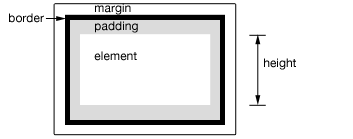
\includegraphics{height.png}
New in version 1.2: 该方法也可以用来得到 windw 和 document 的高度
\begin{Verbatim}[commandchars=\\\{\}]
\PYG{n+nx}{KISSY}\PYG{p}{.}\PYG{n+nx}{use}\PYG{p}{(}\PYG{l+s+s2}{"node"}\PYG{p}{,}\PYG{k+kd}{function}\PYG{p}{(}\PYG{n+nx}{S}\PYG{p}{,}\PYG{n+nx}{Node}\PYG{p}{)}\PYG{p}{\PYGZob{}}
    \PYG{n+nx}{Node}\PYG{p}{.}\PYG{n+nx}{all}\PYG{p}{(}\PYG{n+nb}{window}\PYG{p}{)}\PYG{p}{.}\PYG{n+nx}{height}\PYG{p}{(}\PYG{p}{)}\PYG{p}{;} \PYG{c+c1}{// 得到浏览器可以区域的高度, 相当于 DOM.viewportHeight()}
    \PYG{n+nx}{Node}\PYG{p}{.}\PYG{n+nx}{all}\PYG{p}{(}\PYG{n+nb}{document}\PYG{p}{)}\PYG{p}{.}\PYG{n+nx}{height}\PYG{p}{(}\PYG{p}{)}\PYG{p}{;} \PYG{c+c1}{//得到 html 文档的高度, 相当于 DOM.docHeight()}
\PYG{p}{\PYGZcb{}}\PYG{p}{)}\PYG{p}{;}
\end{Verbatim}

\begin{DUlineblock}{0em}
\item[] NodeList \textbf{height} ( value )
\item[] 设置当前列表每个元素的 css height 值.
\end{DUlineblock}
\begin{quote}\begin{description}
\item[{Parameters}] \leavevmode
\textbf{value} (\emph{number\textbar{}string}) -- 代表像素的整数值, 或数字加上其他单位的字符串值.

\end{description}\end{quote}

\begin{notice}{note}{Note:}
在现代浏览器中, css height 属性不包括 padding , border 或者 margin.
\end{notice}

\end{fulllineitems}



\subparagraph{Demo}
\label{api/core/node/height:demo}
\textbf{得到各种各样的高度, 黄色高亮区域代表 iframe 体}
\begin{quote}

\begin{Verbatim}[commandchars=\\\{\}]
\PYG{c+cp}{\textless{}!DOCTYPE html\textgreater{}}
\PYG{n+nt}{\textless{}html}\PYG{n+nt}{\textgreater{}}
\PYG{n+nt}{\textless{}head}\PYG{n+nt}{\textgreater{}}
  \PYG{n+nt}{\textless{}style}\PYG{n+nt}{\textgreater{}}
  \PYG{n+nt}{body} \PYG{p}{\PYGZob{}} \PYG{k}{background}\PYG{o}{:}\PYG{n+nb}{yellow}\PYG{p}{;} \PYG{p}{\PYGZcb{}}
  \PYG{n+nt}{button} \PYG{p}{\PYGZob{}} \PYG{k}{font-size}\PYG{o}{:}\PYG{l+m}{12px}\PYG{p}{;} \PYG{k}{margin}\PYG{o}{:}\PYG{l+m}{2px}\PYG{p}{;} \PYG{p}{\PYGZcb{}}
  \PYG{n+nt}{p} \PYG{p}{\PYGZob{}} \PYG{k}{width}\PYG{o}{:}\PYG{l+m}{150px}\PYG{p}{;} \PYG{k}{border}\PYG{o}{:}\PYG{l+m}{1px} \PYG{n+nb}{red} \PYG{k}{solid}\PYG{p}{;} \PYG{p}{\PYGZcb{}}
  \PYG{n+nt}{div} \PYG{p}{\PYGZob{}} \PYG{k}{color}\PYG{o}{:}\PYG{n+nb}{red}\PYG{p}{;} \PYG{k}{font-weight}\PYG{o}{:}\PYG{k}{bold}\PYG{p}{;} \PYG{p}{\PYGZcb{}}
  \PYG{n+nt}{\textless{}/style\textgreater{}}
  \PYG{n+nt}{\textless{}script}\PYG{n+nt}{\textgreater{}}
    \PYG{k}{if}\PYG{p}{(}\PYG{n+nx}{location}\PYG{p}{.}\PYG{n+nx}{host}\PYG{o}{==}\PYG{l+s+s2}{"localhost"}\PYG{p}{)}\PYG{p}{\PYGZob{}}
        \PYG{n+nb}{document}\PYG{p}{.}\PYG{n+nx}{writeln}\PYG{p}{(}\PYG{l+s+s1}{'\textless{}script src="http://localhost/kissy\PYGZus{}git/kissy/build/kissy.js"'}\PYG{o}{+}\PYG{l+s+s1}{'\textgreater{}'}\PYG{o}{+}\PYG{l+s+s1}{'\textless{}'}\PYG{o}{+}\PYG{l+s+s1}{'/'}\PYG{o}{+}\PYG{l+s+s1}{'script\textgreater{}'}\PYG{p}{)}\PYG{p}{;}
    \PYG{p}{\PYGZcb{}}\PYG{k}{else}\PYG{p}{\PYGZob{}}
        \PYG{n+nb}{document}\PYG{p}{.}\PYG{n+nx}{writeln}\PYG{p}{(}\PYG{l+s+s1}{'\textless{}script src="http://yiminghe.github.com/kissy/build/kissy.js"'}\PYG{o}{+}\PYG{l+s+s1}{'\textgreater{}'}\PYG{o}{+}\PYG{l+s+s1}{'\textless{}'}\PYG{o}{+}\PYG{l+s+s1}{'/'}\PYG{o}{+}\PYG{l+s+s1}{'script\textgreater{}'}\PYG{p}{)}\PYG{p}{;}
    \PYG{p}{\PYGZcb{}}
   \PYG{n+nt}{\textless{}/script\textgreater{}}
\PYG{n+nt}{\textless{}/head\textgreater{}}
\PYG{n+nt}{\textless{}body}\PYG{n+nt}{\textgreater{}}
  \PYG{n+nt}{\textless{}button} \PYG{n+na}{id=}\PYG{l+s}{"getp"}\PYG{n+nt}{\textgreater{}}Get Paragraph Height\PYG{n+nt}{\textless{}/button\textgreater{}}
  \PYG{n+nt}{\textless{}button} \PYG{n+na}{id=}\PYG{l+s}{"getd"}\PYG{n+nt}{\textgreater{}}Get Document Height\PYG{n+nt}{\textless{}/button\textgreater{}}
  \PYG{n+nt}{\textless{}button} \PYG{n+na}{id=}\PYG{l+s}{"getw"}\PYG{n+nt}{\textgreater{}}Get Window Height\PYG{n+nt}{\textless{}/button\textgreater{}}

  \PYG{n+nt}{\textless{}div}\PYG{n+nt}{\textgreater{}}\PYG{n+ni}{\&nbsp;}\PYG{n+nt}{\textless{}/div\textgreater{}}
  \PYG{n+nt}{\textless{}p}\PYG{n+nt}{\textgreater{}}
    Sample paragraph to test height
  \PYG{n+nt}{\textless{}/p\textgreater{}}
\PYG{n+nt}{\textless{}script}\PYG{n+nt}{\textgreater{}}
    \PYG{n+nx}{KISSY}\PYG{p}{.}\PYG{n+nx}{use}\PYG{p}{(}\PYG{l+s+s2}{"node"}\PYG{p}{,}\PYG{k+kd}{function}\PYG{p}{(}\PYG{n+nx}{S}\PYG{p}{,}\PYG{n+nx}{Node}\PYG{p}{)}\PYG{p}{\PYGZob{}}
        \PYG{k+kd}{var} \PYG{n+nx}{\$}\PYG{o}{=}\PYG{n+nx}{Node}\PYG{p}{.}\PYG{n+nx}{all}\PYG{p}{;}
        \PYG{k+kd}{function} \PYG{n+nx}{showHeight}\PYG{p}{(}\PYG{n+nx}{ele}\PYG{p}{,} \PYG{n+nx}{h}\PYG{p}{)} \PYG{p}{\PYGZob{}}
          \PYG{n+nx}{\$}\PYG{p}{(}\PYG{l+s+s2}{"div"}\PYG{p}{)}\PYG{p}{.}\PYG{n+nx}{text}\PYG{p}{(}\PYG{l+s+s2}{"The height for the "} \PYG{o}{+} \PYG{n+nx}{ele} \PYG{o}{+}
                        \PYG{l+s+s2}{" is "} \PYG{o}{+} \PYG{n+nx}{h} \PYG{o}{+} \PYG{l+s+s2}{"px."}\PYG{p}{)}\PYG{p}{;}
        \PYG{p}{\PYGZcb{}}
        \PYG{n+nx}{\$}\PYG{p}{(}\PYG{l+s+s2}{"\#getp"}\PYG{p}{)}\PYG{p}{.}\PYG{n+nx}{on}\PYG{p}{(}\PYG{l+s+s2}{"click"}\PYG{p}{,}\PYG{k+kd}{function} \PYG{p}{(}\PYG{p}{)} \PYG{p}{\PYGZob{}}
          \PYG{n+nx}{showHeight}\PYG{p}{(}\PYG{l+s+s2}{"paragraph"}\PYG{p}{,} \PYG{n+nx}{\$}\PYG{p}{(}\PYG{l+s+s2}{"p"}\PYG{p}{)}\PYG{p}{.}\PYG{n+nx}{height}\PYG{p}{(}\PYG{p}{)}\PYG{p}{)}\PYG{p}{;}
        \PYG{p}{\PYGZcb{}}\PYG{p}{)}\PYG{p}{;}
        \PYG{n+nx}{\$}\PYG{p}{(}\PYG{l+s+s2}{"\#getd"}\PYG{p}{)}\PYG{p}{.}\PYG{n+nx}{on}\PYG{p}{(}\PYG{l+s+s2}{"click"}\PYG{p}{,}\PYG{k+kd}{function} \PYG{p}{(}\PYG{p}{)} \PYG{p}{\PYGZob{}}
          \PYG{n+nx}{showHeight}\PYG{p}{(}\PYG{l+s+s2}{"document"}\PYG{p}{,} \PYG{n+nx}{\$}\PYG{p}{(}\PYG{n+nb}{document}\PYG{p}{)}\PYG{p}{.}\PYG{n+nx}{height}\PYG{p}{(}\PYG{p}{)}\PYG{p}{)}\PYG{p}{;}
        \PYG{p}{\PYGZcb{}}\PYG{p}{)}\PYG{p}{;}
        \PYG{n+nx}{\$}\PYG{p}{(}\PYG{l+s+s2}{"\#getw"}\PYG{p}{)}\PYG{p}{.}\PYG{n+nx}{on}\PYG{p}{(}\PYG{l+s+s2}{"click"}\PYG{p}{,}\PYG{k+kd}{function} \PYG{p}{(}\PYG{p}{)} \PYG{p}{\PYGZob{}}
          \PYG{n+nx}{showHeight}\PYG{p}{(}\PYG{l+s+s2}{"window"}\PYG{p}{,} \PYG{n+nx}{\$}\PYG{p}{(}\PYG{n+nb}{window}\PYG{p}{)}\PYG{p}{.}\PYG{n+nx}{height}\PYG{p}{(}\PYG{p}{)}\PYG{p}{)}\PYG{p}{;}
        \PYG{p}{\PYGZcb{}}\PYG{p}{)}\PYG{p}{;}
    \PYG{p}{\PYGZcb{}}\PYG{p}{)}\PYG{p}{;}
\PYG{n+nt}{\textless{}/script\textgreater{}}

\PYG{n+nt}{\textless{}/body\textgreater{}}
\PYG{n+nt}{\textless{}/html\textgreater{}}
\end{Verbatim}
\end{quote}

\textbf{设置元素的高度}
\begin{quote}

\begin{Verbatim}[commandchars=\\\{\}]
\PYG{c+cp}{\textless{}!DOCTYPE html\textgreater{}}
\PYG{n+nt}{\textless{}html}\PYG{n+nt}{\textgreater{}}
\PYG{n+nt}{\textless{}head}\PYG{n+nt}{\textgreater{}}
  \PYG{n+nt}{\textless{}style}\PYG{n+nt}{\textgreater{}}\PYG{n+nt}{div} \PYG{p}{\PYGZob{}} \PYG{k}{width}\PYG{o}{:}\PYG{l+m}{50px}\PYG{p}{;} \PYG{k}{height}\PYG{o}{:}\PYG{l+m}{70px}\PYG{p}{;} \PYG{k}{float}\PYG{o}{:}\PYG{k}{left}\PYG{p}{;} \PYG{k}{margin}\PYG{o}{:}\PYG{l+m}{5px}\PYG{p}{;}
        \PYG{k}{background}\PYG{o}{:}\PYG{k}{rgb}\PYG{p}{(}\PYG{l+m}{255}\PYG{o}{,}\PYG{l+m}{140}\PYG{o}{,}\PYG{l+m}{0}\PYG{p}{);} \PYG{k}{cursor}\PYG{o}{:}\PYG{k}{pointer}\PYG{p}{;} \PYG{p}{\PYGZcb{}}  \PYG{n+nt}{\textless{}/style\textgreater{}}
  \PYG{n+nt}{\textless{}script}\PYG{n+nt}{\textgreater{}}
    \PYG{k}{if}\PYG{p}{(}\PYG{n+nx}{location}\PYG{p}{.}\PYG{n+nx}{host}\PYG{o}{==}\PYG{l+s+s2}{"localhost"}\PYG{p}{)}\PYG{p}{\PYGZob{}}
        \PYG{n+nb}{document}\PYG{p}{.}\PYG{n+nx}{writeln}\PYG{p}{(}\PYG{l+s+s1}{'\textless{}script src="http://localhost/kissy\PYGZus{}git/kissy/build/kissy.js"'}\PYG{o}{+}\PYG{l+s+s1}{'\textgreater{}'}\PYG{o}{+}\PYG{l+s+s1}{'\textless{}'}\PYG{o}{+}\PYG{l+s+s1}{'/'}\PYG{o}{+}\PYG{l+s+s1}{'script\textgreater{}'}\PYG{p}{)}\PYG{p}{;}
    \PYG{p}{\PYGZcb{}}\PYG{k}{else}\PYG{p}{\PYGZob{}}
        \PYG{n+nb}{document}\PYG{p}{.}\PYG{n+nx}{writeln}\PYG{p}{(}\PYG{l+s+s1}{'\textless{}script src="http://yiminghe.github.com/kissy/build/kissy.js"'}\PYG{o}{+}\PYG{l+s+s1}{'\textgreater{}'}\PYG{o}{+}\PYG{l+s+s1}{'\textless{}'}\PYG{o}{+}\PYG{l+s+s1}{'/'}\PYG{o}{+}\PYG{l+s+s1}{'script\textgreater{}'}\PYG{p}{)}\PYG{p}{;}
    \PYG{p}{\PYGZcb{}}
   \PYG{n+nt}{\textless{}/script\textgreater{}}
\PYG{n+nt}{\textless{}/head\textgreater{}}
\PYG{n+nt}{\textless{}body}\PYG{n+nt}{\textgreater{}}
  \PYG{n+nt}{\textless{}div}\PYG{n+nt}{\textgreater{}}\PYG{n+nt}{\textless{}/div\textgreater{}}
  \PYG{n+nt}{\textless{}div}\PYG{n+nt}{\textgreater{}}\PYG{n+nt}{\textless{}/div\textgreater{}}

  \PYG{n+nt}{\textless{}div}\PYG{n+nt}{\textgreater{}}\PYG{n+nt}{\textless{}/div\textgreater{}}
  \PYG{n+nt}{\textless{}div}\PYG{n+nt}{\textgreater{}}\PYG{n+nt}{\textless{}/div\textgreater{}}
  \PYG{n+nt}{\textless{}div}\PYG{n+nt}{\textgreater{}}\PYG{n+nt}{\textless{}/div\textgreater{}}
\PYG{n+nt}{\textless{}script}\PYG{n+nt}{\textgreater{}}
    \PYG{n+nx}{KISSY}\PYG{p}{.}\PYG{n+nx}{use}\PYG{p}{(}\PYG{l+s+s2}{"node"}\PYG{p}{,}\PYG{k+kd}{function}\PYG{p}{(}\PYG{n+nx}{S}\PYG{p}{,}\PYG{n+nx}{Node}\PYG{p}{)}\PYG{p}{\PYGZob{}}
        \PYG{k+kd}{var} \PYG{n+nx}{\$}\PYG{o}{=}\PYG{n+nx}{Node}\PYG{p}{.}\PYG{n+nx}{all}\PYG{p}{;}
        \PYG{k+kd}{function} \PYG{n+nx}{handle}\PYG{p}{(}\PYG{p}{)}\PYG{p}{\PYGZob{}}
            \PYG{n+nx}{\$}\PYG{p}{(}\PYG{k}{this}\PYG{p}{)}\PYG{p}{.}\PYG{n+nx}{detach}\PYG{p}{(}\PYG{p}{)}\PYG{p}{;}
            \PYG{n+nx}{\$}\PYG{p}{(}\PYG{k}{this}\PYG{p}{)}\PYG{p}{.}\PYG{n+nx}{height}\PYG{p}{(}\PYG{l+m+mi}{30}\PYG{p}{)}
                 \PYG{p}{.}\PYG{n+nx}{css}\PYG{p}{(}\PYG{p}{\PYGZob{}}\PYG{n+nx}{cursor}\PYG{o}{:}\PYG{l+s+s2}{"auto"}\PYG{p}{,} \PYG{n+nx}{backgroundColor}\PYG{o}{:}\PYG{l+s+s2}{"green"}\PYG{p}{\PYGZcb{}}\PYG{p}{)}\PYG{p}{;}
        \PYG{p}{\PYGZcb{}}
        \PYG{n+nx}{\$}\PYG{p}{(}\PYG{l+s+s2}{"div"}\PYG{p}{)}\PYG{p}{.}\PYG{n+nx}{on}\PYG{p}{(}\PYG{l+s+s1}{'click'}\PYG{p}{,} \PYG{n+nx}{handle}\PYG{p}{)}\PYG{p}{;}
    \PYG{p}{\PYGZcb{}}\PYG{p}{)}\PYG{p}{;}
\PYG{n+nt}{\textless{}/script\textgreater{}}

\PYG{n+nt}{\textless{}/body\textgreater{}}
\PYG{n+nt}{\textless{}/html\textgreater{}}
\end{Verbatim}
\end{quote}


\paragraph{width}
\label{api/core/node/width:width}\label{api/core/node/width::doc}

\subparagraph{Module}
\label{api/core/node/width:module}\begin{quote}

{\hyperref[api/core/node/index:module-Node]{\code{Node}}}
\end{quote}


\subparagraph{Methods}
\label{api/core/node/width:methods}
\index{width() (in module Node)}

\begin{fulllineitems}
\phantomsection\label{api/core/node/width:Node.width}\pysiglinewithargsret{\code{Node.}\bfcode{width}}{}{}~
\begin{DUlineblock}{0em}
\item[] NodeList \textbf{width} ()
\item[] 得到当前节点列表第一个节点的计算宽度
\end{DUlineblock}
\begin{quote}\begin{description}
\item[{Return type}] \leavevmode
number

\end{description}\end{quote}

和 \code{css('width')} 的区别在于该函数返回不带单位的纯数值, 而前者则返回带单位的原始值(例如 \code{400px} ).
当需要数值计算时, 推荐该方法.
New in version 1.2: 该方法也可以用来得到 windw 和 document 的宽度
\begin{Verbatim}[commandchars=\\\{\}]
\PYG{n+nx}{KISSY}\PYG{p}{.}\PYG{n+nx}{use}\PYG{p}{(}\PYG{l+s+s2}{"node"}\PYG{p}{,}\PYG{k+kd}{function}\PYG{p}{(}\PYG{n+nx}{S}\PYG{p}{,}\PYG{n+nx}{Node}\PYG{p}{)}\PYG{p}{\PYGZob{}}
    \PYG{n+nx}{Node}\PYG{p}{.}\PYG{n+nx}{all}\PYG{p}{(}\PYG{n+nb}{window}\PYG{p}{)}\PYG{p}{.}\PYG{n+nx}{width}\PYG{p}{(}\PYG{p}{)}\PYG{p}{;} \PYG{c+c1}{// 得到浏览器可以区域的高度, 相当于 DOM.viewportWidth()}
    \PYG{n+nx}{Node}\PYG{p}{.}\PYG{n+nx}{all}\PYG{p}{(}\PYG{n+nb}{document}\PYG{p}{)}\PYG{p}{.}\PYG{n+nx}{width}\PYG{p}{(}\PYG{p}{)}\PYG{p}{;} \PYG{c+c1}{//得到 html 文档的高度, 相当于 DOM.docWidth()}
\PYG{p}{\PYGZcb{}}\PYG{p}{)}\PYG{p}{;}
\end{Verbatim}

\begin{DUlineblock}{0em}
\item[] NodeList \textbf{width} ( value )
\item[] 设置当前列表每个元素的 css width 值.
\end{DUlineblock}
\begin{quote}\begin{description}
\item[{Parameters}] \leavevmode
\textbf{value} (\emph{number\textbar{}string}) -- 代表像素的整数值, 或数字加上其他单位的字符串值.

\end{description}\end{quote}

\begin{notice}{note}{Note:}
在现代浏览器中, css width 属性不包括 padding , border 或者 margin.
\end{notice}

例子可参考 {\hyperref[api/core/node/height:Node.height]{\code{height()}}}

\end{fulllineitems}



\paragraph{addStyleSheet}
\label{api/core/node/addStyleSheet:addstylesheet}\label{api/core/node/addStyleSheet::doc}New in version 1.2.

\subparagraph{Module}
\label{api/core/node/addStyleSheet:module}\begin{quote}

{\hyperref[api/core/node/index:module-Node]{\code{Node}}}
\end{quote}


\subparagraph{Methods}
\label{api/core/node/addStyleSheet:methods}
\index{addStyleSheet() (in module Node)}

\begin{fulllineitems}
\phantomsection\label{api/core/node/addStyleSheet:Node.addStyleSheet}\pysiglinewithargsret{\code{Node.}\bfcode{addStyleSheet}}{}{}~
\begin{DUlineblock}{0em}
\item[] NodeList \textbf{addStyleSheet} (cssText{[}, id{]})
\item[] 将 cssText 字符串作为内联样式添加到文档中.
\end{DUlineblock}
\begin{quote}\begin{description}
\item[{Parameters}] \leavevmode\begin{itemize}
\item {}
\textbf{cssText} (\emph{string}) -- 样式内容

\item {}
\textbf{id} (\emph{string}) -- 内联样式所在 style 节点的 id

\end{itemize}

\item[{Return type}] \leavevmode
NodeList

\item[{Returns}] \leavevmode
当前对象

\end{description}\end{quote}

\begin{notice}{note}{Note:}
该方法只可以在 window 和 document 上调用, 例如:

\begin{Verbatim}[commandchars=\\\{\}]
\PYG{n+nx}{KISSY}\PYG{p}{.}\PYG{n+nx}{use}\PYG{p}{(}\PYG{l+s+s2}{"node"}\PYG{p}{,}\PYG{k+kd}{function}\PYG{p}{(}\PYG{n+nx}{S}\PYG{p}{,}\PYG{n+nx}{Node}\PYG{p}{)}\PYG{p}{\PYGZob{}}
    \PYG{k+kd}{var} \PYG{n+nx}{\$}\PYG{o}{=}\PYG{n+nx}{Node}\PYG{p}{.}\PYG{n+nx}{all}\PYG{p}{;}
    \PYG{n+nx}{\$}\PYG{p}{(}\PYG{n+nb}{window}\PYG{p}{)}\PYG{p}{.}\PYG{n+nx}{addStyleSheet}\PYG{p}{(}\PYG{l+s+s2}{"p \PYGZob{}color:red;\PYGZcb{}"}\PYG{p}{)}\PYG{p}{;} \PYG{c+c1}{// 段落颜色全部显示为红色}
    \PYG{c+c1}{// 或}
    \PYG{n+nx}{\$}\PYG{p}{(}\PYG{n+nb}{document}\PYG{p}{)}\PYG{p}{.}\PYG{n+nx}{addStyleSheet}\PYG{p}{(}\PYG{l+s+s2}{"p \PYGZob{}color:red;\PYGZcb{}"}\PYG{p}{,}\PYG{l+s+s2}{"addCss"}\PYG{p}{)}\PYG{p}{;}
\PYG{p}{\PYGZcb{}}\PYG{p}{)}\PYG{p}{;}
\end{Verbatim}
\end{notice}

\end{fulllineitems}



\paragraph{append}
\label{api/core/node/append::doc}\label{api/core/node/append:append}

\subparagraph{Module}
\label{api/core/node/append:module}\begin{quote}

{\hyperref[api/core/node/index:module-Node]{\code{Node}}}
\end{quote}


\subparagraph{Methods}
\label{api/core/node/append:methods}
\index{append() (in module Node)}

\begin{fulllineitems}
\phantomsection\label{api/core/node/append:Node.append}\pysiglinewithargsret{\code{Node.}\bfcode{append}}{}{}~
\begin{DUlineblock}{0em}
\item[] NodeList \textbf{animate} ( content )
\item[] 将参数内容插入到当前节点列表中的每个元素的末尾.
\end{DUlineblock}
\begin{quote}\begin{description}
\item[{Parameters}] \leavevmode
\textbf{content} (\emph{HTMLELement\textbar{}string\textbar{}NodeList}) -- 将要插入的内容

\item[{Return type}] \leavevmode
NodeList

\end{description}\end{quote}

该方法插入指定内容到当前节点列表的最后一个元素后面(如果要插入到第一个元素前面, 请用 \code{prepend()} ).

该方法和 \code{appendTo()} 功能一样. 最大的区别在于语法不同以及参数意义不同. 当使用 \code{append} 方法时, 当前节点列表为参数内容的插入容器.
而对于 \code{appendTo}  当前节点列表则为要插入的元素, 而参数则为目标容器.

例如:

\begin{Verbatim}[commandchars=\\\{\}]
\PYG{n+nt}{\textless{}h2}\PYG{n+nt}{\textgreater{}}Greetings\PYG{n+nt}{\textless{}/h2\textgreater{}}
\PYG{n+nt}{\textless{}div} \PYG{n+na}{class=}\PYG{l+s}{"container"}\PYG{n+nt}{\textgreater{}}
  \PYG{n+nt}{\textless{}div} \PYG{n+na}{class=}\PYG{l+s}{"inner"}\PYG{n+nt}{\textgreater{}}Hello\PYG{n+nt}{\textless{}/div\textgreater{}}
  \PYG{n+nt}{\textless{}div} \PYG{n+na}{class=}\PYG{l+s}{"inner"}\PYG{n+nt}{\textgreater{}}Goodbye\PYG{n+nt}{\textless{}/div\textgreater{}}
\PYG{n+nt}{\textless{}/div\textgreater{}}
\end{Verbatim}

你可以创建 NodeList 并把它立即插入到指定容器中:

\begin{Verbatim}[commandchars=\\\{\}]
\PYG{n+nx}{KISSY}\PYG{p}{.}\PYG{n+nx}{use}\PYG{p}{(}\PYG{l+s+s2}{"node"}\PYG{p}{,}\PYG{k+kd}{function}\PYG{p}{(}\PYG{n+nx}{S}\PYG{p}{,}\PYG{n+nx}{NodeList}\PYG{p}{)}\PYG{p}{\PYGZob{}}
    \PYG{n+nx}{NodeList}\PYG{p}{.}\PYG{n+nx}{all}\PYG{p}{(}\PYG{l+s+s1}{'.inner'}\PYG{p}{)}\PYG{p}{.}\PYG{n+nx}{append}\PYG{p}{(}\PYG{l+s+s1}{'\textless{}p\textgreater{}Test\textless{}/p\textgreater{}'}\PYG{p}{)}\PYG{p}{;}
\PYG{p}{\PYGZcb{}}\PYG{p}{)}\PYG{p}{;}
\end{Verbatim}

内层的每个 div 元素都得到了新内容

\begin{Verbatim}[commandchars=\\\{\}]
\PYG{n+nt}{\textless{}h2}\PYG{n+nt}{\textgreater{}}Greetings\PYG{n+nt}{\textless{}/h2\textgreater{}}
\PYG{n+nt}{\textless{}div} \PYG{n+na}{class=}\PYG{l+s}{"container"}\PYG{n+nt}{\textgreater{}}
  \PYG{n+nt}{\textless{}div} \PYG{n+na}{class=}\PYG{l+s}{"inner"}\PYG{n+nt}{\textgreater{}}
    Hello
    \PYG{n+nt}{\textless{}p}\PYG{n+nt}{\textgreater{}}Test\PYG{n+nt}{\textless{}/p\textgreater{}}
  \PYG{n+nt}{\textless{}/div\textgreater{}}
  \PYG{n+nt}{\textless{}div} \PYG{n+na}{class=}\PYG{l+s}{"inner"}\PYG{n+nt}{\textgreater{}}
    Goodbye
    \PYG{n+nt}{\textless{}p}\PYG{n+nt}{\textgreater{}}Test\PYG{n+nt}{\textless{}/p\textgreater{}}
  \PYG{n+nt}{\textless{}/div\textgreater{}}
\PYG{n+nt}{\textless{}/div\textgreater{}}
\end{Verbatim}

你可以把页面上已有的元素 \code{prepend} 到另外一个:

\begin{Verbatim}[commandchars=\\\{\}]
\PYG{n+nx}{KISSY}\PYG{p}{.}\PYG{n+nx}{use}\PYG{p}{(}\PYG{l+s+s2}{"node"}\PYG{p}{,}\PYG{k+kd}{function}\PYG{p}{(}\PYG{n+nx}{S}\PYG{p}{,}\PYG{n+nx}{NodeList}\PYG{p}{)}\PYG{p}{\PYGZob{}}
    \PYG{n+nx}{NodeList}\PYG{p}{.}\PYG{n+nx}{all}\PYG{p}{(}\PYG{l+s+s1}{'.container'}\PYG{p}{)}\PYG{p}{.}\PYG{n+nx}{append}\PYG{p}{(}\PYG{n+nx}{\$}\PYG{p}{(}\PYG{l+s+s1}{'h2'}\PYG{p}{)}\PYG{p}{)}\PYG{p}{;}
\PYG{p}{\PYGZcb{}}\PYG{p}{)}\PYG{p}{;}
\end{Verbatim}

如果当前节点列表只包括一个节点, 那么他将会被移到目标容器中(而不是克隆):

\begin{Verbatim}[commandchars=\\\{\}]
\PYG{n+nt}{\textless{}div} \PYG{n+na}{class=}\PYG{l+s}{"container"}\PYG{n+nt}{\textgreater{}}
  \PYG{n+nt}{\textless{}div} \PYG{n+na}{class=}\PYG{l+s}{"inner"}\PYG{n+nt}{\textgreater{}}Hello\PYG{n+nt}{\textless{}/div\textgreater{}}
  \PYG{n+nt}{\textless{}div} \PYG{n+na}{class=}\PYG{l+s}{"inner"}\PYG{n+nt}{\textgreater{}}Goodbye\PYG{n+nt}{\textless{}/div\textgreater{}}
  \PYG{n+nt}{\textless{}h2}\PYG{n+nt}{\textgreater{}}Greetings\PYG{n+nt}{\textless{}/h2\textgreater{}}
\PYG{n+nt}{\textless{}/div\textgreater{}}
\end{Verbatim}

但是如果当前节点列表包括多余一个节点, 则除了第一个节点外, 其他节点都添加的是参数节点的克隆节点.

\end{fulllineitems}



\subparagraph{Demo}
\label{api/core/node/append:demo}
\textbf{在所有段落中添加一些 html 字符串}
\begin{quote}

\begin{Verbatim}[commandchars=\\\{\}]
    \PYG{c+cp}{\textless{}!DOCTYPE html\textgreater{}}
    \PYG{n+nt}{\textless{}html}\PYG{n+nt}{\textgreater{}}
    \PYG{n+nt}{\textless{}head}\PYG{n+nt}{\textgreater{}}
      \PYG{n+nt}{\textless{}style}\PYG{n+nt}{\textgreater{}}
      \PYG{n+nt}{p} \PYG{p}{\PYGZob{}} \PYG{k}{background}\PYG{o}{:}\PYG{n+nb}{yellow}\PYG{p}{;} \PYG{p}{\PYGZcb{}}
    \PYG{n+nt}{\textless{}/style\textgreater{}}
     \PYG{n+nt}{\textless{}script}\PYG{n+nt}{\textgreater{}}
    \PYG{k}{if}\PYG{p}{(}\PYG{n+nx}{location}\PYG{p}{.}\PYG{n+nx}{host}\PYG{o}{==}\PYG{l+s+s2}{"localhost"}\PYG{p}{)}\PYG{p}{\PYGZob{}}
        \PYG{n+nb}{document}\PYG{p}{.}\PYG{n+nx}{writeln}\PYG{p}{(}\PYG{l+s+s1}{'\textless{}script src="http://localhost/kissy\PYGZus{}git/kissy/build/kissy.js"'}\PYG{o}{+}\PYG{l+s+s1}{'\textgreater{}'}\PYG{o}{+}\PYG{l+s+s1}{'\textless{}'}\PYG{o}{+}\PYG{l+s+s1}{'/'}\PYG{o}{+}\PYG{l+s+s1}{'script\textgreater{}'}\PYG{p}{)}\PYG{p}{;}
    \PYG{p}{\PYGZcb{}}\PYG{k}{else}\PYG{p}{\PYGZob{}}
        \PYG{n+nb}{document}\PYG{p}{.}\PYG{n+nx}{writeln}\PYG{p}{(}\PYG{l+s+s1}{'\textless{}script src="http://yiminghe.github.com/kissy/build/kissy.js"'}\PYG{o}{+}\PYG{l+s+s1}{'\textgreater{}'}\PYG{o}{+}\PYG{l+s+s1}{'\textless{}'}\PYG{o}{+}\PYG{l+s+s1}{'/'}\PYG{o}{+}\PYG{l+s+s1}{'script\textgreater{}'}\PYG{p}{)}\PYG{p}{;}
    \PYG{p}{\PYGZcb{}}
   \PYG{n+nt}{\textless{}/script\textgreater{}}
    \PYG{n+nt}{\textless{}/head\textgreater{}}
    \PYG{n+nt}{\textless{}body}\PYG{n+nt}{\textgreater{}}
      \PYG{n+nt}{\textless{}p}\PYG{n+nt}{\textgreater{}} is I would like to say \PYG{n+nt}{\textless{}/p\textgreater{}}
    \PYG{n+nt}{\textless{}script}\PYG{n+nt}{\textgreater{}}
        \PYG{n+nx}{KISSY}\PYG{p}{.}\PYG{n+nx}{use}\PYG{p}{(}\PYG{l+s+s2}{"node"}\PYG{p}{,}\PYG{k+kd}{function}\PYG{p}{(}\PYG{n+nx}{S}\PYG{p}{,}\PYG{n+nx}{NodeList}\PYG{p}{)}\PYG{p}{\PYGZob{}}
            \PYG{n+nx}{NodeList}\PYG{p}{.}\PYG{n+nx}{all}\PYG{p}{(}\PYG{l+s+s2}{"p"}\PYG{p}{)}\PYG{p}{.}\PYG{n+nx}{append}\PYG{p}{(}\PYG{l+s+s2}{"\textless{}strong\textgreater{}Hello\textless{}/strong\textgreater{}"}\PYG{p}{)}\PYG{p}{;}
        \PYG{p}{\PYGZcb{}}\PYG{p}{)}\PYG{p}{;}
    \PYG{n+nt}{\textless{}/script\textgreater{}}

    \PYG{n+nt}{\textless{}/body\textgreater{}}
    \PYG{n+nt}{\textless{}/html\textgreater{}}
\end{Verbatim}
\end{quote}

\textbf{给所有段落添加一个文本节点}
\begin{quote}

\begin{Verbatim}[commandchars=\\\{\}]
    \PYG{c+cp}{\textless{}!DOCTYPE html\textgreater{}}
    \PYG{n+nt}{\textless{}html}\PYG{n+nt}{\textgreater{}}
    \PYG{n+nt}{\textless{}head}\PYG{n+nt}{\textgreater{}}
      \PYG{n+nt}{\textless{}style}\PYG{n+nt}{\textgreater{}}
      \PYG{n+nt}{p} \PYG{p}{\PYGZob{}} \PYG{k}{background}\PYG{o}{:}\PYG{n+nb}{yellow}\PYG{p}{;} \PYG{p}{\PYGZcb{}}
    \PYG{n+nt}{\textless{}/style\textgreater{}}
     \PYG{n+nt}{\textless{}script}\PYG{n+nt}{\textgreater{}}
    \PYG{k}{if}\PYG{p}{(}\PYG{n+nx}{location}\PYG{p}{.}\PYG{n+nx}{host}\PYG{o}{==}\PYG{l+s+s2}{"localhost"}\PYG{p}{)}\PYG{p}{\PYGZob{}}
        \PYG{n+nb}{document}\PYG{p}{.}\PYG{n+nx}{writeln}\PYG{p}{(}\PYG{l+s+s1}{'\textless{}script src="http://localhost/kissy\PYGZus{}git/kissy/build/kissy.js"'}\PYG{o}{+}\PYG{l+s+s1}{'\textgreater{}'}\PYG{o}{+}\PYG{l+s+s1}{'\textless{}'}\PYG{o}{+}\PYG{l+s+s1}{'/'}\PYG{o}{+}\PYG{l+s+s1}{'script\textgreater{}'}\PYG{p}{)}\PYG{p}{;}
    \PYG{p}{\PYGZcb{}}\PYG{k}{else}\PYG{p}{\PYGZob{}}
        \PYG{n+nb}{document}\PYG{p}{.}\PYG{n+nx}{writeln}\PYG{p}{(}\PYG{l+s+s1}{'\textless{}script src="http://yiminghe.github.com/kissy/build/kissy.js"'}\PYG{o}{+}\PYG{l+s+s1}{'\textgreater{}'}\PYG{o}{+}\PYG{l+s+s1}{'\textless{}'}\PYG{o}{+}\PYG{l+s+s1}{'/'}\PYG{o}{+}\PYG{l+s+s1}{'script\textgreater{}'}\PYG{p}{)}\PYG{p}{;}
    \PYG{p}{\PYGZcb{}}
   \PYG{n+nt}{\textless{}/script\textgreater{}}
    \PYG{n+nt}{\textless{}/head\textgreater{}}
    \PYG{n+nt}{\textless{}body}\PYG{n+nt}{\textgreater{}}
      \PYG{n+nt}{\textless{}p}\PYG{n+nt}{\textgreater{}}I would like to say: \PYG{n+nt}{\textless{}/p\textgreater{}}
      \PYG{n+nt}{\textless{}p}\PYG{n+nt}{\textgreater{}}I also would like to say: \PYG{n+nt}{\textless{}/p\textgreater{}}
    \PYG{n+nt}{\textless{}script}\PYG{n+nt}{\textgreater{}}
        \PYG{n+nx}{KISSY}\PYG{p}{.}\PYG{n+nx}{use}\PYG{p}{(}\PYG{l+s+s2}{"node"}\PYG{p}{,}\PYG{k+kd}{function}\PYG{p}{(}\PYG{n+nx}{S}\PYG{p}{,}\PYG{n+nx}{NodeList}\PYG{p}{)}\PYG{p}{\PYGZob{}}
            \PYG{n+nx}{NodeList}\PYG{p}{.}\PYG{n+nx}{all}\PYG{p}{(}\PYG{l+s+s2}{"p"}\PYG{p}{)}\PYG{p}{.}\PYG{n+nx}{append}\PYG{p}{(}\PYG{n+nb}{document}\PYG{p}{.}\PYG{n+nx}{createTextNode}\PYG{p}{(}\PYG{l+s+s2}{"Hello"}\PYG{p}{)}\PYG{p}{)}\PYG{p}{;}
        \PYG{p}{\PYGZcb{}}\PYG{p}{)}\PYG{p}{;}
    \PYG{n+nt}{\textless{}/script\textgreater{}}

    \PYG{n+nt}{\textless{}/body\textgreater{}}
    \PYG{n+nt}{\textless{}/html\textgreater{}}
\end{Verbatim}
\end{quote}

\textbf{给所有段落添加一个 {}`{}`NodeList{}`{}`  对象}
\begin{quote}

\begin{Verbatim}[commandchars=\\\{\}]
    \PYG{c+cp}{\textless{}!DOCTYPE html\textgreater{}}
    \PYG{n+nt}{\textless{}html}\PYG{n+nt}{\textgreater{}}
    \PYG{n+nt}{\textless{}head}\PYG{n+nt}{\textgreater{}}
      \PYG{n+nt}{\textless{}style}\PYG{n+nt}{\textgreater{}}
      \PYG{n+nt}{p} \PYG{p}{\PYGZob{}} \PYG{k}{background}\PYG{o}{:}\PYG{n+nb}{yellow}\PYG{p}{;} \PYG{p}{\PYGZcb{}}
    \PYG{n+nt}{\textless{}/style\textgreater{}}
     \PYG{n+nt}{\textless{}script}\PYG{n+nt}{\textgreater{}}
    \PYG{k}{if}\PYG{p}{(}\PYG{n+nx}{location}\PYG{p}{.}\PYG{n+nx}{host}\PYG{o}{==}\PYG{l+s+s2}{"localhost"}\PYG{p}{)}\PYG{p}{\PYGZob{}}
        \PYG{n+nb}{document}\PYG{p}{.}\PYG{n+nx}{writeln}\PYG{p}{(}\PYG{l+s+s1}{'\textless{}script src="http://localhost/kissy\PYGZus{}git/kissy/build/kissy.js"'}\PYG{o}{+}\PYG{l+s+s1}{'\textgreater{}'}\PYG{o}{+}\PYG{l+s+s1}{'\textless{}'}\PYG{o}{+}\PYG{l+s+s1}{'/'}\PYG{o}{+}\PYG{l+s+s1}{'script\textgreater{}'}\PYG{p}{)}\PYG{p}{;}
    \PYG{p}{\PYGZcb{}}\PYG{k}{else}\PYG{p}{\PYGZob{}}
        \PYG{n+nb}{document}\PYG{p}{.}\PYG{n+nx}{writeln}\PYG{p}{(}\PYG{l+s+s1}{'\textless{}script src="http://yiminghe.github.com/kissy/build/kissy.js"'}\PYG{o}{+}\PYG{l+s+s1}{'\textgreater{}'}\PYG{o}{+}\PYG{l+s+s1}{'\textless{}'}\PYG{o}{+}\PYG{l+s+s1}{'/'}\PYG{o}{+}\PYG{l+s+s1}{'script\textgreater{}'}\PYG{p}{)}\PYG{p}{;}
    \PYG{p}{\PYGZcb{}}
   \PYG{n+nt}{\textless{}/script\textgreater{}}
    \PYG{n+nt}{\textless{}/head\textgreater{}}
    \PYG{n+nt}{\textless{}body}\PYG{n+nt}{\textgreater{}}
        \PYG{n+nt}{\textless{}strong}\PYG{n+nt}{\textgreater{}}Hello world!!!\PYG{n+nt}{\textless{}/strong\textgreater{}}\PYG{n+nt}{\textless{}p}\PYG{n+nt}{\textgreater{}}I would like to say: \PYG{n+nt}{\textless{}/p\textgreater{}}

    \PYG{n+nt}{\textless{}script}\PYG{n+nt}{\textgreater{}}
        \PYG{n+nx}{KISSY}\PYG{p}{.}\PYG{n+nx}{use}\PYG{p}{(}\PYG{l+s+s2}{"node"}\PYG{p}{,}\PYG{k+kd}{function}\PYG{p}{(}\PYG{n+nx}{S}\PYG{p}{,}\PYG{n+nx}{NodeList}\PYG{p}{)}\PYG{p}{\PYGZob{}}
            \PYG{n+nx}{NodeList}\PYG{p}{.}\PYG{n+nx}{all}\PYG{p}{(}\PYG{l+s+s2}{"p"}\PYG{p}{)}\PYG{p}{.}\PYG{n+nx}{append}\PYG{p}{(}\PYG{n+nx}{NodeList}\PYG{p}{.}\PYG{n+nx}{all}\PYG{p}{(}\PYG{l+s+s2}{"strong"}\PYG{p}{)}\PYG{p}{)}\PYG{p}{;}
        \PYG{p}{\PYGZcb{}}\PYG{p}{)}\PYG{p}{;}
    \PYG{n+nt}{\textless{}/script\textgreater{}}

    \PYG{n+nt}{\textless{}/body\textgreater{}}
    \PYG{n+nt}{\textless{}/html\textgreater{}}
\end{Verbatim}
\end{quote}


\paragraph{appendTo}
\label{api/core/node/appendTo:appendto}\label{api/core/node/appendTo::doc}

\subparagraph{Module}
\label{api/core/node/appendTo:module}\begin{quote}

{\hyperref[api/core/node/index:module-Node]{\code{Node}}}
\end{quote}


\subparagraph{Methods}
\label{api/core/node/appendTo:methods}
\index{appendTo() (in module Node)}

\begin{fulllineitems}
\phantomsection\label{api/core/node/appendTo:Node.appendTo}\pysiglinewithargsret{\code{Node.}\bfcode{appendTo}}{}{}~
\begin{DUlineblock}{0em}
\item[] NodeList \textbf{appendTo} ( containers )
\item[] 将当前节点列表中的每个元素插入到容器列表的每个元素的最后一个子节点后面.
\end{DUlineblock}
\begin{quote}\begin{description}
\item[{Parameters}] \leavevmode
\textbf{content} (\emph{HTMLELement\textbar{}string\textbar{}NodeList}) --
将要插入的内容
\begin{itemize}
\item {}
HTMLELement\textbar{}NodeList: 已有或新创建的节点

\item {}
string: 选择器字符串, 查找已有的容器节点

\end{itemize}


\item[{Return type}] \leavevmode
NodeList

\end{description}\end{quote}

\code{appendTo} 和 \code{append()} 功能一样, 只不过参数意义不同.

考虑下面 html 字符串:

\begin{Verbatim}[commandchars=\\\{\}]
\PYG{n+nt}{\textless{}h2}\PYG{n+nt}{\textgreater{}}Greetings\PYG{n+nt}{\textless{}/h2\textgreater{}}
\PYG{n+nt}{\textless{}div} \PYG{n+na}{class=}\PYG{l+s}{"container"}\PYG{n+nt}{\textgreater{}}
  \PYG{n+nt}{\textless{}div} \PYG{n+na}{class=}\PYG{l+s}{"inner"}\PYG{n+nt}{\textgreater{}}Hello\PYG{n+nt}{\textless{}/div\textgreater{}}
  \PYG{n+nt}{\textless{}div} \PYG{n+na}{class=}\PYG{l+s}{"inner"}\PYG{n+nt}{\textgreater{}}Goodbye\PYG{n+nt}{\textless{}/div\textgreater{}}
\PYG{n+nt}{\textless{}/div\textgreater{}}
\end{Verbatim}

我们可以创建元素后立即插入到多个已有元素:

\begin{Verbatim}[commandchars=\\\{\}]
\PYG{n+nx}{NodeList}\PYG{p}{.}\PYG{n+nx}{all}\PYG{p}{(}\PYG{l+s+s1}{'\textless{}p\textgreater{}Test\textless{}/p\textgreater{}'}\PYG{p}{)}\PYG{p}{.}\PYG{n+nx}{appendTo}\PYG{p}{(}\PYG{l+s+s1}{'.inner'}\PYG{p}{)}\PYG{p}{;}
\end{Verbatim}

每个内层 div 元素都得到了新内容

\begin{Verbatim}[commandchars=\\\{\}]
\PYG{n+nt}{\textless{}h2}\PYG{n+nt}{\textgreater{}}Greetings\PYG{n+nt}{\textless{}/h2\textgreater{}}
\PYG{n+nt}{\textless{}div} \PYG{n+na}{class=}\PYG{l+s}{"container"}\PYG{n+nt}{\textgreater{}}
  \PYG{n+nt}{\textless{}div} \PYG{n+na}{class=}\PYG{l+s}{"inner"}\PYG{n+nt}{\textgreater{}}
    Hello
    \PYG{n+nt}{\textless{}p}\PYG{n+nt}{\textgreater{}}Test\PYG{n+nt}{\textless{}/p\textgreater{}}
  \PYG{n+nt}{\textless{}/div\textgreater{}}
  \PYG{n+nt}{\textless{}div} \PYG{n+na}{class=}\PYG{l+s}{"inner"}\PYG{n+nt}{\textgreater{}}
    Goodbye
    \PYG{n+nt}{\textless{}p}\PYG{n+nt}{\textgreater{}}Test\PYG{n+nt}{\textless{}/p\textgreater{}}
  \PYG{n+nt}{\textless{}/div\textgreater{}}
\PYG{n+nt}{\textless{}/div\textgreater{}}
\end{Verbatim}

我们也可以把一个已有元素插入到另一个

\begin{Verbatim}[commandchars=\\\{\}]
\PYG{n+nx}{NodeList}\PYG{p}{.}\PYG{n+nx}{all}\PYG{p}{(}\PYG{l+s+s1}{'h2'}\PYG{p}{)}\PYG{p}{.}\PYG{n+nx}{appendTo}\PYG{p}{(}\PYG{n+nx}{NodeList}\PYG{p}{.}\PYG{n+nx}{all}\PYG{p}{(}\PYG{l+s+s1}{'.container'}\PYG{p}{)}\PYG{p}{)}\PYG{p}{;}
\end{Verbatim}

如果容器列表只有一个节点, 那么当前节点列表会被移动到容器内(不是克隆):

\begin{Verbatim}[commandchars=\\\{\}]
\PYG{n+nt}{\textless{}div} \PYG{n+na}{class=}\PYG{l+s}{"container"}\PYG{n+nt}{\textgreater{}}
  \PYG{n+nt}{\textless{}div} \PYG{n+na}{class=}\PYG{l+s}{"inner"}\PYG{n+nt}{\textgreater{}}Hello\PYG{n+nt}{\textless{}/div\textgreater{}}
  \PYG{n+nt}{\textless{}div} \PYG{n+na}{class=}\PYG{l+s}{"inner"}\PYG{n+nt}{\textgreater{}}Goodbye\PYG{n+nt}{\textless{}/div\textgreater{}}
  \PYG{n+nt}{\textless{}h2}\PYG{n+nt}{\textgreater{}}Greetings\PYG{n+nt}{\textless{}/h2\textgreater{}}
\PYG{n+nt}{\textless{}/div\textgreater{}}
\end{Verbatim}

不过如果有多个目标容器, 那么除了第一个目标容器, 当前节点列表的复制节点会被插入到其他目标容器

\end{fulllineitems}



\subparagraph{Demo}
\label{api/core/node/appendTo:demo}
\textbf{把多个 span 插入到已有元素}
\begin{quote}

\begin{Verbatim}[commandchars=\\\{\}]
\PYG{c+cp}{\textless{}!DOCTYPE html\textgreater{}}
\PYG{n+nt}{\textless{}html}\PYG{n+nt}{\textgreater{}}
\PYG{n+nt}{\textless{}head}\PYG{n+nt}{\textgreater{}}
  \PYG{n+nt}{\textless{}style}\PYG{n+nt}{\textgreater{}}\PYG{n+nt}{div} \PYG{p}{\PYGZob{}} \PYG{k}{background}\PYG{o}{:}\PYG{n+nb}{yellow}\PYG{p}{;} \PYG{p}{\PYGZcb{}}\PYG{n+nt}{\textless{}/style\textgreater{}}
  \PYG{n+nt}{\textless{}script}\PYG{n+nt}{\textgreater{}}
    \PYG{k}{if}\PYG{p}{(}\PYG{n+nx}{location}\PYG{p}{.}\PYG{n+nx}{host}\PYG{o}{==}\PYG{l+s+s2}{"localhost"}\PYG{p}{)}\PYG{p}{\PYGZob{}}
        \PYG{n+nb}{document}\PYG{p}{.}\PYG{n+nx}{writeln}\PYG{p}{(}\PYG{l+s+s1}{'\textless{}script src="http://localhost/kissy\PYGZus{}git/kissy/build/kissy.js"'}\PYG{o}{+}\PYG{l+s+s1}{'\textgreater{}'}\PYG{o}{+}\PYG{l+s+s1}{'\textless{}'}\PYG{o}{+}\PYG{l+s+s1}{'/'}\PYG{o}{+}\PYG{l+s+s1}{'script\textgreater{}'}\PYG{p}{)}\PYG{p}{;}
    \PYG{p}{\PYGZcb{}}\PYG{k}{else}\PYG{p}{\PYGZob{}}
        \PYG{n+nb}{document}\PYG{p}{.}\PYG{n+nx}{writeln}\PYG{p}{(}\PYG{l+s+s1}{'\textless{}script src="http://yiminghe.github.com/kissy/build/kissy.js"'}\PYG{o}{+}\PYG{l+s+s1}{'\textgreater{}'}\PYG{o}{+}\PYG{l+s+s1}{'\textless{}'}\PYG{o}{+}\PYG{l+s+s1}{'/'}\PYG{o}{+}\PYG{l+s+s1}{'script\textgreater{}'}\PYG{p}{)}\PYG{p}{;}
    \PYG{p}{\PYGZcb{}}
   \PYG{n+nt}{\textless{}/script\textgreater{}}
\PYG{n+nt}{\textless{}/head\textgreater{}}
\PYG{n+nt}{\textless{}body}\PYG{n+nt}{\textgreater{}}
    \PYG{n+nt}{\textless{}div} \PYG{n+na}{id=}\PYG{l+s}{"foo"}\PYG{n+nt}{\textgreater{}}FOO! is \PYG{n+nt}{\textless{}/div\textgreater{}}

    \PYG{n+nt}{\textless{}span}\PYG{n+nt}{\textgreater{}}I have something to say... \PYG{n+nt}{\textless{}/span\textgreater{}}

    \PYG{n+nt}{\textless{}span}\PYG{n+nt}{\textgreater{}} once more : \PYG{n+nt}{\textless{}/span\textgreater{}}

    \PYG{n+nt}{\textless{}script}\PYG{n+nt}{\textgreater{}}
        \PYG{n+nx}{KISSY}\PYG{p}{.}\PYG{n+nx}{use}\PYG{p}{(}\PYG{l+s+s2}{"node"}\PYG{p}{,}\PYG{k+kd}{function}\PYG{p}{(}\PYG{n+nx}{S}\PYG{p}{,}\PYG{n+nx}{NodeList}\PYG{p}{)}\PYG{p}{\PYGZob{}}
            \PYG{n+nx}{NodeList}\PYG{p}{.}\PYG{n+nx}{all}\PYG{p}{(}\PYG{l+s+s2}{"span"}\PYG{p}{)}\PYG{p}{.}\PYG{n+nx}{appendTo}\PYG{p}{(}\PYG{n+nx}{NodeList}\PYG{p}{.}\PYG{n+nx}{all}\PYG{p}{(}\PYG{l+s+s2}{"\#foo"}\PYG{p}{)}\PYG{p}{)}\PYG{p}{;}
        \PYG{p}{\PYGZcb{}}\PYG{p}{)}\PYG{p}{;}
    \PYG{n+nt}{\textless{}/script\textgreater{}}
\PYG{n+nt}{\textless{}/body\textgreater{}}
\PYG{n+nt}{\textless{}/html\textgreater{}}
\end{Verbatim}
\end{quote}


\paragraph{prepend}
\label{api/core/node/prepend::doc}\label{api/core/node/prepend:prepend}

\subparagraph{Module}
\label{api/core/node/prepend:module}\begin{quote}

{\hyperref[api/core/node/index:module-Node]{\code{Node}}}
\end{quote}


\subparagraph{Methods}
\label{api/core/node/prepend:methods}
\index{prepend() (in module Node)}

\begin{fulllineitems}
\phantomsection\label{api/core/node/prepend:Node.prepend}\pysiglinewithargsret{\code{Node.}\bfcode{prepend}}{}{}~
\begin{DUlineblock}{0em}
\item[] NodeList \textbf{prepend} ( content )
\item[] 将参数内容插入到当前节点列表中的每个元素的开头.
\end{DUlineblock}
\begin{quote}\begin{description}
\item[{Parameters}] \leavevmode
\textbf{content} (\emph{HTMLELement\textbar{}string\textbar{}NodeList}) -- 将要插入的内容

\item[{Return type}] \leavevmode
NodeList

\end{description}\end{quote}

该方法插入指定内容到当前节点列表的第一个元素前面(如果要插入到最后一个元素后面, 请用 \code{append()} ).

\begin{notice}{note}{Note:}
该方法和 \code{prependTo()} 功能一样. 最大的区别在于语法不同以及参数意义不同. 当使用 \code{prepend} 方法时, 当前节点列表为参数内容的插入容器.
而对于 \code{prependTo}  当前节点列表则为要插入的元素, 而参数则为目标容器.
\end{notice}

\begin{Verbatim}[commandchars=\\\{\}]
\PYG{n+nt}{\textless{}h2}\PYG{n+nt}{\textgreater{}}Greetings\PYG{n+nt}{\textless{}/h2\textgreater{}}
\PYG{n+nt}{\textless{}div} \PYG{n+na}{class=}\PYG{l+s}{"container"}\PYG{n+nt}{\textgreater{}}
  \PYG{n+nt}{\textless{}div} \PYG{n+na}{class=}\PYG{l+s}{"inner"}\PYG{n+nt}{\textgreater{}}Hello\PYG{n+nt}{\textless{}/div\textgreater{}}
  \PYG{n+nt}{\textless{}div} \PYG{n+na}{class=}\PYG{l+s}{"inner"}\PYG{n+nt}{\textgreater{}}Goodbye\PYG{n+nt}{\textless{}/div\textgreater{}}
\PYG{n+nt}{\textless{}/div\textgreater{}}
\end{Verbatim}

你可以创建 NodeList 并把它立即插入到指定容器中:

\begin{Verbatim}[commandchars=\\\{\}]
\PYG{n+nx}{KISSY}\PYG{p}{.}\PYG{n+nx}{use}\PYG{p}{(}\PYG{l+s+s2}{"node"}\PYG{p}{,}\PYG{k+kd}{function}\PYG{p}{(}\PYG{n+nx}{S}\PYG{p}{,}\PYG{n+nx}{NodeList}\PYG{p}{)}\PYG{p}{\PYGZob{}}
    \PYG{n+nx}{NodeList}\PYG{p}{.}\PYG{n+nx}{all}\PYG{p}{(}\PYG{l+s+s1}{'.inner'}\PYG{p}{)}\PYG{p}{.}\PYG{n+nx}{prepend}\PYG{p}{(}\PYG{l+s+s1}{'\textless{}p\textgreater{}Test\textless{}/p\textgreater{}'}\PYG{p}{)}\PYG{p}{;}
\PYG{p}{\PYGZcb{}}\PYG{p}{)}\PYG{p}{;}
\end{Verbatim}

内层的每个 div 元素都得到了新内容

\begin{Verbatim}[commandchars=\\\{\}]
\PYG{n+nt}{\textless{}h2}\PYG{n+nt}{\textgreater{}}Greetings\PYG{n+nt}{\textless{}/h2\textgreater{}}
\PYG{n+nt}{\textless{}div} \PYG{n+na}{class=}\PYG{l+s}{"container"}\PYG{n+nt}{\textgreater{}}
  \PYG{n+nt}{\textless{}div} \PYG{n+na}{class=}\PYG{l+s}{"inner"}\PYG{n+nt}{\textgreater{}}
    \PYG{n+nt}{\textless{}p}\PYG{n+nt}{\textgreater{}}Test\PYG{n+nt}{\textless{}/p\textgreater{}}
    Hello
  \PYG{n+nt}{\textless{}/div\textgreater{}}
  \PYG{n+nt}{\textless{}div} \PYG{n+na}{class=}\PYG{l+s}{"inner"}\PYG{n+nt}{\textgreater{}}
    \PYG{n+nt}{\textless{}p}\PYG{n+nt}{\textgreater{}}Test\PYG{n+nt}{\textless{}/p\textgreater{}}
    Goodbye
  \PYG{n+nt}{\textless{}/div\textgreater{}}
\PYG{n+nt}{\textless{}/div\textgreater{}}
\end{Verbatim}

你可以把页面上已有的元素 \code{prepend} 到另外一个:

\begin{Verbatim}[commandchars=\\\{\}]
\PYG{n+nx}{KISSY}\PYG{p}{.}\PYG{n+nx}{use}\PYG{p}{(}\PYG{l+s+s2}{"node"}\PYG{p}{,}\PYG{k+kd}{function}\PYG{p}{(}\PYG{n+nx}{S}\PYG{p}{,}\PYG{n+nx}{NodeList}\PYG{p}{)}\PYG{p}{\PYGZob{}}
    \PYG{n+nx}{NodeList}\PYG{p}{.}\PYG{n+nx}{all}\PYG{p}{(}\PYG{l+s+s1}{'.container'}\PYG{p}{)}\PYG{p}{.}\PYG{n+nx}{prepend}\PYG{p}{(}\PYG{n+nx}{\$}\PYG{p}{(}\PYG{l+s+s1}{'h2'}\PYG{p}{)}\PYG{p}{)}\PYG{p}{;}
\PYG{p}{\PYGZcb{}}\PYG{p}{)}\PYG{p}{;}
\end{Verbatim}

如果当前节点列表只包括一个节点, 那么他将会被移到目标容器中(而不是克隆):

\begin{Verbatim}[commandchars=\\\{\}]
\PYG{n+nt}{\textless{}div} \PYG{n+na}{class=}\PYG{l+s}{"container"}\PYG{n+nt}{\textgreater{}}
    \PYG{n+nt}{\textless{}h2}\PYG{n+nt}{\textgreater{}}Greetings\PYG{n+nt}{\textless{}/h2\textgreater{}}
    \PYG{n+nt}{\textless{}div} \PYG{n+na}{class=}\PYG{l+s}{"inner"}\PYG{n+nt}{\textgreater{}}Hello\PYG{n+nt}{\textless{}/div\textgreater{}}
    \PYG{n+nt}{\textless{}div} \PYG{n+na}{class=}\PYG{l+s}{"inner"}\PYG{n+nt}{\textgreater{}}Goodbye\PYG{n+nt}{\textless{}/div\textgreater{}}
\PYG{n+nt}{\textless{}/div\textgreater{}}
\end{Verbatim}

但是如果当前节点列表包括多余一个节点, 则除了第一个节点外, 其他节点都添加的是参数节点的克隆节点.

\end{fulllineitems}



\subparagraph{Demo}
\label{api/core/node/prepend:demo}
\textbf{在所有段落中添加一些 html 字符串}
\begin{quote}

\begin{Verbatim}[commandchars=\\\{\}]
    \PYG{c+cp}{\textless{}!DOCTYPE html\textgreater{}}
    \PYG{n+nt}{\textless{}html}\PYG{n+nt}{\textgreater{}}
    \PYG{n+nt}{\textless{}head}\PYG{n+nt}{\textgreater{}}
      \PYG{n+nt}{\textless{}style}\PYG{n+nt}{\textgreater{}}
      \PYG{n+nt}{p} \PYG{p}{\PYGZob{}} \PYG{k}{background}\PYG{o}{:}\PYG{n+nb}{yellow}\PYG{p}{;} \PYG{p}{\PYGZcb{}}
    \PYG{n+nt}{\textless{}/style\textgreater{}}
     \PYG{n+nt}{\textless{}script}\PYG{n+nt}{\textgreater{}}
    \PYG{k}{if}\PYG{p}{(}\PYG{n+nx}{location}\PYG{p}{.}\PYG{n+nx}{host}\PYG{o}{==}\PYG{l+s+s2}{"localhost"}\PYG{p}{)}\PYG{p}{\PYGZob{}}
        \PYG{n+nb}{document}\PYG{p}{.}\PYG{n+nx}{writeln}\PYG{p}{(}\PYG{l+s+s1}{'\textless{}script src="http://localhost/kissy\PYGZus{}git/kissy/build/kissy.js"'}\PYG{o}{+}\PYG{l+s+s1}{'\textgreater{}'}\PYG{o}{+}\PYG{l+s+s1}{'\textless{}'}\PYG{o}{+}\PYG{l+s+s1}{'/'}\PYG{o}{+}\PYG{l+s+s1}{'script\textgreater{}'}\PYG{p}{)}\PYG{p}{;}
    \PYG{p}{\PYGZcb{}}\PYG{k}{else}\PYG{p}{\PYGZob{}}
        \PYG{n+nb}{document}\PYG{p}{.}\PYG{n+nx}{writeln}\PYG{p}{(}\PYG{l+s+s1}{'\textless{}script src="http://yiminghe.github.com/kissy/build/kissy.js"'}\PYG{o}{+}\PYG{l+s+s1}{'\textgreater{}'}\PYG{o}{+}\PYG{l+s+s1}{'\textless{}'}\PYG{o}{+}\PYG{l+s+s1}{'/'}\PYG{o}{+}\PYG{l+s+s1}{'script\textgreater{}'}\PYG{p}{)}\PYG{p}{;}
    \PYG{p}{\PYGZcb{}}
   \PYG{n+nt}{\textless{}/script\textgreater{}}
    \PYG{n+nt}{\textless{}/head\textgreater{}}
    \PYG{n+nt}{\textless{}body}\PYG{n+nt}{\textgreater{}}
      \PYG{n+nt}{\textless{}p}\PYG{n+nt}{\textgreater{}}I would like to say: \PYG{n+nt}{\textless{}/p\textgreater{}}
    \PYG{n+nt}{\textless{}script}\PYG{n+nt}{\textgreater{}}
        \PYG{n+nx}{KISSY}\PYG{p}{.}\PYG{n+nx}{use}\PYG{p}{(}\PYG{l+s+s2}{"node"}\PYG{p}{,}\PYG{k+kd}{function}\PYG{p}{(}\PYG{n+nx}{S}\PYG{p}{,}\PYG{n+nx}{NodeList}\PYG{p}{)}\PYG{p}{\PYGZob{}}
            \PYG{n+nx}{NodeList}\PYG{p}{.}\PYG{n+nx}{all}\PYG{p}{(}\PYG{l+s+s2}{"p"}\PYG{p}{)}\PYG{p}{.}\PYG{n+nx}{prepend}\PYG{p}{(}\PYG{l+s+s2}{"\textless{}strong\textgreater{}Hello\textless{}/strong\textgreater{}"}\PYG{p}{)}\PYG{p}{;}
        \PYG{p}{\PYGZcb{}}\PYG{p}{)}\PYG{p}{;}
    \PYG{n+nt}{\textless{}/script\textgreater{}}

    \PYG{n+nt}{\textless{}/body\textgreater{}}
    \PYG{n+nt}{\textless{}/html\textgreater{}}
\end{Verbatim}
\end{quote}

\textbf{给所有段落添加一个文本节点}
\begin{quote}

\begin{Verbatim}[commandchars=\\\{\}]
    \PYG{c+cp}{\textless{}!DOCTYPE html\textgreater{}}
    \PYG{n+nt}{\textless{}html}\PYG{n+nt}{\textgreater{}}
    \PYG{n+nt}{\textless{}head}\PYG{n+nt}{\textgreater{}}
      \PYG{n+nt}{\textless{}style}\PYG{n+nt}{\textgreater{}}
      \PYG{n+nt}{p} \PYG{p}{\PYGZob{}} \PYG{k}{background}\PYG{o}{:}\PYG{n+nb}{yellow}\PYG{p}{;} \PYG{p}{\PYGZcb{}}
    \PYG{n+nt}{\textless{}/style\textgreater{}}
     \PYG{n+nt}{\textless{}script}\PYG{n+nt}{\textgreater{}}
    \PYG{k}{if}\PYG{p}{(}\PYG{n+nx}{location}\PYG{p}{.}\PYG{n+nx}{host}\PYG{o}{==}\PYG{l+s+s2}{"localhost"}\PYG{p}{)}\PYG{p}{\PYGZob{}}
        \PYG{n+nb}{document}\PYG{p}{.}\PYG{n+nx}{writeln}\PYG{p}{(}\PYG{l+s+s1}{'\textless{}script src="http://localhost/kissy\PYGZus{}git/kissy/build/kissy.js"'}\PYG{o}{+}\PYG{l+s+s1}{'\textgreater{}'}\PYG{o}{+}\PYG{l+s+s1}{'\textless{}'}\PYG{o}{+}\PYG{l+s+s1}{'/'}\PYG{o}{+}\PYG{l+s+s1}{'script\textgreater{}'}\PYG{p}{)}\PYG{p}{;}
    \PYG{p}{\PYGZcb{}}\PYG{k}{else}\PYG{p}{\PYGZob{}}
        \PYG{n+nb}{document}\PYG{p}{.}\PYG{n+nx}{writeln}\PYG{p}{(}\PYG{l+s+s1}{'\textless{}script src="http://yiminghe.github.com/kissy/build/kissy.js"'}\PYG{o}{+}\PYG{l+s+s1}{'\textgreater{}'}\PYG{o}{+}\PYG{l+s+s1}{'\textless{}'}\PYG{o}{+}\PYG{l+s+s1}{'/'}\PYG{o}{+}\PYG{l+s+s1}{'script\textgreater{}'}\PYG{p}{)}\PYG{p}{;}
    \PYG{p}{\PYGZcb{}}
   \PYG{n+nt}{\textless{}/script\textgreater{}}
    \PYG{n+nt}{\textless{}/head\textgreater{}}
    \PYG{n+nt}{\textless{}body}\PYG{n+nt}{\textgreater{}}
      \PYG{n+nt}{\textless{}p}\PYG{n+nt}{\textgreater{}} is I would like to say \PYG{n+nt}{\textless{}/p\textgreater{}}
      \PYG{n+nt}{\textless{}p}\PYG{n+nt}{\textgreater{}} is also I would like to say\PYG{n+nt}{\textless{}/p\textgreater{}}
    \PYG{n+nt}{\textless{}script}\PYG{n+nt}{\textgreater{}}
        \PYG{n+nx}{KISSY}\PYG{p}{.}\PYG{n+nx}{use}\PYG{p}{(}\PYG{l+s+s2}{"node"}\PYG{p}{,}\PYG{k+kd}{function}\PYG{p}{(}\PYG{n+nx}{S}\PYG{p}{,}\PYG{n+nx}{NodeList}\PYG{p}{)}\PYG{p}{\PYGZob{}}
            \PYG{n+nx}{NodeList}\PYG{p}{.}\PYG{n+nx}{all}\PYG{p}{(}\PYG{l+s+s2}{"p"}\PYG{p}{)}\PYG{p}{.}\PYG{n+nx}{prepend}\PYG{p}{(}\PYG{n+nb}{document}\PYG{p}{.}\PYG{n+nx}{createTextNode}\PYG{p}{(}\PYG{l+s+s2}{"Hello"}\PYG{p}{)}\PYG{p}{)}\PYG{p}{;}
        \PYG{p}{\PYGZcb{}}\PYG{p}{)}\PYG{p}{;}
    \PYG{n+nt}{\textless{}/script\textgreater{}}

    \PYG{n+nt}{\textless{}/body\textgreater{}}
    \PYG{n+nt}{\textless{}/html\textgreater{}}
\end{Verbatim}
\end{quote}

\textbf{给所有段落添加一个 {}`{}`NodeList{}`{}`  对象}
\begin{quote}

\begin{Verbatim}[commandchars=\\\{\}]
    \PYG{c+cp}{\textless{}!DOCTYPE html\textgreater{}}
    \PYG{n+nt}{\textless{}html}\PYG{n+nt}{\textgreater{}}
    \PYG{n+nt}{\textless{}head}\PYG{n+nt}{\textgreater{}}
      \PYG{n+nt}{\textless{}style}\PYG{n+nt}{\textgreater{}}
      \PYG{n+nt}{p} \PYG{p}{\PYGZob{}} \PYG{k}{background}\PYG{o}{:}\PYG{n+nb}{yellow}\PYG{p}{;} \PYG{p}{\PYGZcb{}}
    \PYG{n+nt}{\textless{}/style\textgreater{}}
     \PYG{n+nt}{\textless{}script}\PYG{n+nt}{\textgreater{}}
    \PYG{k}{if}\PYG{p}{(}\PYG{n+nx}{location}\PYG{p}{.}\PYG{n+nx}{host}\PYG{o}{==}\PYG{l+s+s2}{"localhost"}\PYG{p}{)}\PYG{p}{\PYGZob{}}
        \PYG{n+nb}{document}\PYG{p}{.}\PYG{n+nx}{writeln}\PYG{p}{(}\PYG{l+s+s1}{'\textless{}script src="http://localhost/kissy\PYGZus{}git/kissy/build/kissy.js"'}\PYG{o}{+}\PYG{l+s+s1}{'\textgreater{}'}\PYG{o}{+}\PYG{l+s+s1}{'\textless{}'}\PYG{o}{+}\PYG{l+s+s1}{'/'}\PYG{o}{+}\PYG{l+s+s1}{'script\textgreater{}'}\PYG{p}{)}\PYG{p}{;}
    \PYG{p}{\PYGZcb{}}\PYG{k}{else}\PYG{p}{\PYGZob{}}
        \PYG{n+nb}{document}\PYG{p}{.}\PYG{n+nx}{writeln}\PYG{p}{(}\PYG{l+s+s1}{'\textless{}script src="http://yiminghe.github.com/kissy/build/kissy.js"'}\PYG{o}{+}\PYG{l+s+s1}{'\textgreater{}'}\PYG{o}{+}\PYG{l+s+s1}{'\textless{}'}\PYG{o}{+}\PYG{l+s+s1}{'/'}\PYG{o}{+}\PYG{l+s+s1}{'script\textgreater{}'}\PYG{p}{)}\PYG{p}{;}
    \PYG{p}{\PYGZcb{}}
   \PYG{n+nt}{\textless{}/script\textgreater{}}
    \PYG{n+nt}{\textless{}/head\textgreater{}}
    \PYG{n+nt}{\textless{}body}\PYG{n+nt}{\textgreater{}}
       \PYG{n+nt}{\textless{}p}\PYG{n+nt}{\textgreater{}} is I would like to say \PYG{n+nt}{\textless{}/p\textgreater{}} \PYG{n+nt}{\textless{}strong}\PYG{n+nt}{\textgreater{}}Hello world!!!\PYG{n+nt}{\textless{}/strong\textgreater{}}

    \PYG{n+nt}{\textless{}script}\PYG{n+nt}{\textgreater{}}
        \PYG{n+nx}{KISSY}\PYG{p}{.}\PYG{n+nx}{use}\PYG{p}{(}\PYG{l+s+s2}{"node"}\PYG{p}{,}\PYG{k+kd}{function}\PYG{p}{(}\PYG{n+nx}{S}\PYG{p}{,}\PYG{n+nx}{NodeList}\PYG{p}{)}\PYG{p}{\PYGZob{}}
            \PYG{n+nx}{NodeList}\PYG{p}{.}\PYG{n+nx}{all}\PYG{p}{(}\PYG{l+s+s2}{"p"}\PYG{p}{)}\PYG{p}{.}\PYG{n+nx}{prepend}\PYG{p}{(}\PYG{n+nx}{NodeList}\PYG{p}{.}\PYG{n+nx}{all}\PYG{p}{(}\PYG{l+s+s2}{"strong"}\PYG{p}{)}\PYG{p}{)}\PYG{p}{;}
        \PYG{p}{\PYGZcb{}}\PYG{p}{)}\PYG{p}{;}
    \PYG{n+nt}{\textless{}/script\textgreater{}}

    \PYG{n+nt}{\textless{}/body\textgreater{}}
    \PYG{n+nt}{\textless{}/html\textgreater{}}
\end{Verbatim}
\end{quote}


\paragraph{prependTo}
\label{api/core/node/prependTo:prependto}\label{api/core/node/prependTo::doc}

\subparagraph{Module}
\label{api/core/node/prependTo:module}\begin{quote}

{\hyperref[api/core/node/index:module-Node]{\code{Node}}}
\end{quote}


\subparagraph{Methods}
\label{api/core/node/prependTo:methods}
\index{prependTo() (in module Node)}

\begin{fulllineitems}
\phantomsection\label{api/core/node/prependTo:Node.prependTo}\pysiglinewithargsret{\code{Node.}\bfcode{prependTo}}{}{}~
\begin{DUlineblock}{0em}
\item[] NodeList \textbf{prependTo} ( containers )
\item[] 将当前节点列表中的每个元素插入到容器列表的每个元素的开头.
\end{DUlineblock}
\begin{quote}\begin{description}
\item[{Parameters}] \leavevmode
\textbf{content} (\emph{HTMLELement\textbar{}string\textbar{}NodeList}) --
将要插入的内容
\begin{itemize}
\item {}
HTMLELement\textbar{}NodeList: 已有或新创建的节点

\item {}
string: 选择器字符串, 查找已有的容器节点

\end{itemize}


\item[{Return type}] \leavevmode
NodeList

\end{description}\end{quote}

\code{prependTo} 和 \code{prepend()} 功能一样, 只不过参数意义不同.

考虑下面 html 字符串:

\begin{Verbatim}[commandchars=\\\{\}]
\PYG{n+nt}{\textless{}h2}\PYG{n+nt}{\textgreater{}}Greetings\PYG{n+nt}{\textless{}/h2\textgreater{}}
\PYG{n+nt}{\textless{}div} \PYG{n+na}{class=}\PYG{l+s}{"container"}\PYG{n+nt}{\textgreater{}}
  \PYG{n+nt}{\textless{}div} \PYG{n+na}{class=}\PYG{l+s}{"inner"}\PYG{n+nt}{\textgreater{}}Hello\PYG{n+nt}{\textless{}/div\textgreater{}}
  \PYG{n+nt}{\textless{}div} \PYG{n+na}{class=}\PYG{l+s}{"inner"}\PYG{n+nt}{\textgreater{}}Goodbye\PYG{n+nt}{\textless{}/div\textgreater{}}
\PYG{n+nt}{\textless{}/div\textgreater{}}
\end{Verbatim}

我们可以创建元素后立即插入到多个已有元素:

\begin{Verbatim}[commandchars=\\\{\}]
\PYG{n+nx}{NodeList}\PYG{p}{.}\PYG{n+nx}{all}\PYG{p}{(}\PYG{l+s+s1}{'\textless{}p\textgreater{}Test\textless{}/p\textgreater{}'}\PYG{p}{)}\PYG{p}{.}\PYG{n+nx}{prependTo}\PYG{p}{(}\PYG{l+s+s1}{'.inner'}\PYG{p}{)}\PYG{p}{;}
\end{Verbatim}

每个内层 div 元素都得到了新内容

\begin{Verbatim}[commandchars=\\\{\}]
\PYG{n+nt}{\textless{}h2}\PYG{n+nt}{\textgreater{}}Greetings\PYG{n+nt}{\textless{}/h2\textgreater{}}
\PYG{n+nt}{\textless{}div} \PYG{n+na}{class=}\PYG{l+s}{"container"}\PYG{n+nt}{\textgreater{}}
  \PYG{n+nt}{\textless{}div} \PYG{n+na}{class=}\PYG{l+s}{"inner"}\PYG{n+nt}{\textgreater{}}
    \PYG{n+nt}{\textless{}p}\PYG{n+nt}{\textgreater{}}Test\PYG{n+nt}{\textless{}/p\textgreater{}}
    Hello
  \PYG{n+nt}{\textless{}/div\textgreater{}}
  \PYG{n+nt}{\textless{}div} \PYG{n+na}{class=}\PYG{l+s}{"inner"}\PYG{n+nt}{\textgreater{}}
    \PYG{n+nt}{\textless{}p}\PYG{n+nt}{\textgreater{}}Test\PYG{n+nt}{\textless{}/p\textgreater{}}
    Goodbye
  \PYG{n+nt}{\textless{}/div\textgreater{}}
\PYG{n+nt}{\textless{}/div\textgreater{}}
\end{Verbatim}

我们也可以把一个已有元素插入到另一个

\begin{Verbatim}[commandchars=\\\{\}]
\PYG{n+nx}{NodeList}\PYG{p}{.}\PYG{n+nx}{all}\PYG{p}{(}\PYG{l+s+s1}{'h2'}\PYG{p}{)}\PYG{p}{.}\PYG{n+nx}{prependTo}\PYG{p}{(}\PYG{n+nx}{NodeList}\PYG{p}{.}\PYG{n+nx}{all}\PYG{p}{(}\PYG{l+s+s1}{'.container'}\PYG{p}{)}\PYG{p}{)}\PYG{p}{;}
\end{Verbatim}

如果容器列表只有一个节点, 那么当前节点列表会被移动到容器内(不是克隆):

\begin{Verbatim}[commandchars=\\\{\}]
\PYG{n+nt}{\textless{}div} \PYG{n+na}{class=}\PYG{l+s}{"container"}\PYG{n+nt}{\textgreater{}}
  \PYG{n+nt}{\textless{}h2}\PYG{n+nt}{\textgreater{}}Greetings\PYG{n+nt}{\textless{}/h2\textgreater{}}
  \PYG{n+nt}{\textless{}div} \PYG{n+na}{class=}\PYG{l+s}{"inner"}\PYG{n+nt}{\textgreater{}}Hello\PYG{n+nt}{\textless{}/div\textgreater{}}
  \PYG{n+nt}{\textless{}div} \PYG{n+na}{class=}\PYG{l+s}{"inner"}\PYG{n+nt}{\textgreater{}}Goodbye\PYG{n+nt}{\textless{}/div\textgreater{}}
\PYG{n+nt}{\textless{}/div\textgreater{}}
\end{Verbatim}

不过如果有多个目标容器, 那么除了第一个目标容器, 当前节点列表的复制节点会被插入到其他目标容器

\end{fulllineitems}



\subparagraph{Demo}
\label{api/core/node/prependTo:demo}
\textbf{把多个 span 插入到已有元素}
\begin{quote}

\begin{Verbatim}[commandchars=\\\{\}]
\PYG{c+cp}{\textless{}!DOCTYPE html\textgreater{}}
\PYG{n+nt}{\textless{}html}\PYG{n+nt}{\textgreater{}}
\PYG{n+nt}{\textless{}head}\PYG{n+nt}{\textgreater{}}
  \PYG{n+nt}{\textless{}style}\PYG{n+nt}{\textgreater{}}\PYG{n+nt}{div} \PYG{p}{\PYGZob{}} \PYG{k}{background}\PYG{o}{:}\PYG{n+nb}{yellow}\PYG{p}{;} \PYG{p}{\PYGZcb{}}\PYG{n+nt}{\textless{}/style\textgreater{}}
  \PYG{n+nt}{\textless{}script}\PYG{n+nt}{\textgreater{}}
    \PYG{k}{if}\PYG{p}{(}\PYG{n+nx}{location}\PYG{p}{.}\PYG{n+nx}{host}\PYG{o}{==}\PYG{l+s+s2}{"localhost"}\PYG{p}{)}\PYG{p}{\PYGZob{}}
        \PYG{n+nb}{document}\PYG{p}{.}\PYG{n+nx}{writeln}\PYG{p}{(}\PYG{l+s+s1}{'\textless{}script src="http://localhost/kissy\PYGZus{}git/kissy/build/kissy.js"'}\PYG{o}{+}\PYG{l+s+s1}{'\textgreater{}'}\PYG{o}{+}\PYG{l+s+s1}{'\textless{}'}\PYG{o}{+}\PYG{l+s+s1}{'/'}\PYG{o}{+}\PYG{l+s+s1}{'script\textgreater{}'}\PYG{p}{)}\PYG{p}{;}
    \PYG{p}{\PYGZcb{}}\PYG{k}{else}\PYG{p}{\PYGZob{}}
        \PYG{n+nb}{document}\PYG{p}{.}\PYG{n+nx}{writeln}\PYG{p}{(}\PYG{l+s+s1}{'\textless{}script src="http://yiminghe.github.com/kissy/build/kissy.js"'}\PYG{o}{+}\PYG{l+s+s1}{'\textgreater{}'}\PYG{o}{+}\PYG{l+s+s1}{'\textless{}'}\PYG{o}{+}\PYG{l+s+s1}{'/'}\PYG{o}{+}\PYG{l+s+s1}{'script\textgreater{}'}\PYG{p}{)}\PYG{p}{;}
    \PYG{p}{\PYGZcb{}}
   \PYG{n+nt}{\textless{}/script\textgreater{}}
\PYG{n+nt}{\textless{}/head\textgreater{}}
\PYG{n+nt}{\textless{}body}\PYG{n+nt}{\textgreater{}}
    \PYG{n+nt}{\textless{}div} \PYG{n+na}{id=}\PYG{l+s}{"foo"}\PYG{n+nt}{\textgreater{}}FOO!\PYG{n+nt}{\textless{}/div\textgreater{}}

    \PYG{n+nt}{\textless{}span}\PYG{n+nt}{\textgreater{}}I have something to say... \PYG{n+nt}{\textless{}/span\textgreater{}}

    \PYG{n+nt}{\textless{}span}\PYG{n+nt}{\textgreater{}} once more : \PYG{n+nt}{\textless{}/span\textgreater{}}

    \PYG{n+nt}{\textless{}script}\PYG{n+nt}{\textgreater{}}
        \PYG{n+nx}{KISSY}\PYG{p}{.}\PYG{n+nx}{use}\PYG{p}{(}\PYG{l+s+s2}{"node"}\PYG{p}{,}\PYG{k+kd}{function}\PYG{p}{(}\PYG{n+nx}{S}\PYG{p}{,}\PYG{n+nx}{NodeList}\PYG{p}{)}\PYG{p}{\PYGZob{}}
            \PYG{n+nx}{NodeList}\PYG{p}{.}\PYG{n+nx}{all}\PYG{p}{(}\PYG{l+s+s2}{"span"}\PYG{p}{)}\PYG{p}{.}\PYG{n+nx}{prependTo}\PYG{p}{(}\PYG{n+nx}{NodeList}\PYG{p}{.}\PYG{n+nx}{all}\PYG{p}{(}\PYG{l+s+s2}{"\#foo"}\PYG{p}{)}\PYG{p}{)}\PYG{p}{;}
        \PYG{p}{\PYGZcb{}}\PYG{p}{)}\PYG{p}{;}
    \PYG{n+nt}{\textless{}/script\textgreater{}}
\PYG{n+nt}{\textless{}/body\textgreater{}}
\PYG{n+nt}{\textless{}/html\textgreater{}}
\end{Verbatim}
\end{quote}


\paragraph{insertBefore}
\label{api/core/node/insertBefore::doc}\label{api/core/node/insertBefore:insertbefore}

\subparagraph{Module}
\label{api/core/node/insertBefore:module}\begin{quote}

{\hyperref[api/core/node/index:module-Node]{\code{Node}}}
\end{quote}


\subparagraph{Methods}
\label{api/core/node/insertBefore:methods}
\index{insertBefore() (in module Node)}

\begin{fulllineitems}
\phantomsection\label{api/core/node/insertBefore:Node.insertBefore}\pysiglinewithargsret{\code{Node.}\bfcode{insertBefore}}{}{}~
\begin{DUlineblock}{0em}
\item[] NodeList \textbf{insertBefore} ( target )
\item[] 将当前列表中的每个元素插入到目标元素之前.
\end{DUlineblock}
\begin{quote}\begin{description}
\item[{Parameters}] \leavevmode
\textbf{target} (\emph{HTMLElement\textbar{}string\textbar{}NodeList}) --
将要插入的元素
\begin{itemize}
\item {}
string : 选择器字符串

\item {}
HTMLElement\textbar{}NodeList : 已有或新建的元素

\end{itemize}


\end{description}\end{quote}

{\hyperref[api/core/node/before:Node.before]{\code{before()}}} 和该方法的功能一样, 只不过参数意义不同, 该函数表示当前节点列表被插入到参数目标节点之前,
而 \code{before} 则表示参数节点被插入到当前节点之前.

\begin{Verbatim}[commandchars=\\\{\}]
\PYG{n+nt}{\textless{}div} \PYG{n+na}{class=}\PYG{l+s}{"container"}\PYG{n+nt}{\textgreater{}}
  \PYG{n+nt}{\textless{}h2}\PYG{n+nt}{\textgreater{}}Greetings\PYG{n+nt}{\textless{}/h2\textgreater{}}
  \PYG{n+nt}{\textless{}div} \PYG{n+na}{class=}\PYG{l+s}{"inner"}\PYG{n+nt}{\textgreater{}}Hello\PYG{n+nt}{\textless{}/div\textgreater{}}
  \PYG{n+nt}{\textless{}div} \PYG{n+na}{class=}\PYG{l+s}{"inner"}\PYG{n+nt}{\textgreater{}}Goodbye\PYG{n+nt}{\textless{}/div\textgreater{}}
\PYG{n+nt}{\textless{}/div\textgreater{}}
\end{Verbatim}

我们可以创建节点并立即把它插入到一些元素之前

\begin{Verbatim}[commandchars=\\\{\}]
\PYG{n+nx}{NodeList}\PYG{p}{.}\PYG{n+nx}{all}\PYG{p}{(}\PYG{l+s+s1}{'\textless{}p\textgreater{}Test\textless{}/p\textgreater{}'}\PYG{p}{)}\PYG{p}{.}\PYG{n+nx}{insertBefore}\PYG{p}{(}\PYG{l+s+s1}{'.inner'}\PYG{p}{)}\PYG{p}{;}
\end{Verbatim}

结果为

\begin{Verbatim}[commandchars=\\\{\}]
\PYG{n+nt}{\textless{}div} \PYG{n+na}{class=}\PYG{l+s}{"container"}\PYG{n+nt}{\textgreater{}}
  \PYG{n+nt}{\textless{}h2}\PYG{n+nt}{\textgreater{}}Greetings\PYG{n+nt}{\textless{}/h2\textgreater{}}
  \PYG{n+nt}{\textless{}p}\PYG{n+nt}{\textgreater{}}Test\PYG{n+nt}{\textless{}/p\textgreater{}}
  \PYG{n+nt}{\textless{}div} \PYG{n+na}{class=}\PYG{l+s}{"inner"}\PYG{n+nt}{\textgreater{}}Hello\PYG{n+nt}{\textless{}/div\textgreater{}}
  \PYG{n+nt}{\textless{}p}\PYG{n+nt}{\textgreater{}}Test\PYG{n+nt}{\textless{}/p\textgreater{}}
  \PYG{n+nt}{\textless{}div} \PYG{n+na}{class=}\PYG{l+s}{"inner"}\PYG{n+nt}{\textgreater{}}Goodbye\PYG{n+nt}{\textless{}/div\textgreater{}}
\PYG{n+nt}{\textless{}/div\textgreater{}}
\end{Verbatim}

我们也可以操纵现有元素

\begin{Verbatim}[commandchars=\\\{\}]
\PYG{n+nx}{NodeList}\PYG{p}{.}\PYG{n+nx}{all}\PYG{p}{(}\PYG{l+s+s1}{'h2'}\PYG{p}{)}\PYG{p}{.}\PYG{n+nx}{insertBefore}\PYG{p}{(}\PYG{n+nx}{NodeList}\PYG{p}{.}\PYG{n+nx}{all}\PYG{p}{(}\PYG{l+s+s1}{'.container'}\PYG{p}{)}\PYG{p}{)}\PYG{p}{;}
\end{Verbatim}

如果目标节点只有一个, 那么当前节点就会移动到目标节点之前

\begin{Verbatim}[commandchars=\\\{\}]
\PYG{n+nt}{\textless{}h2}\PYG{n+nt}{\textgreater{}}Greetings\PYG{n+nt}{\textless{}/h2\textgreater{}}
\PYG{n+nt}{\textless{}div} \PYG{n+na}{class=}\PYG{l+s}{"container"}\PYG{n+nt}{\textgreater{}}
  \PYG{n+nt}{\textless{}div} \PYG{n+na}{class=}\PYG{l+s}{"inner"}\PYG{n+nt}{\textgreater{}}Hello\PYG{n+nt}{\textless{}/div\textgreater{}}
  \PYG{n+nt}{\textless{}div} \PYG{n+na}{class=}\PYG{l+s}{"inner"}\PYG{n+nt}{\textgreater{}}Goodbye\PYG{n+nt}{\textless{}/div\textgreater{}}
\PYG{n+nt}{\textless{}/div\textgreater{}}
\end{Verbatim}

如果有多个目标节点, 那么除了第一个目标节点外, 其他目标节点前会被插入当前节点的克隆

\end{fulllineitems}



\subparagraph{Demo}
\label{api/core/node/insertBefore:demo}\begin{quote}

把段落插入到 div 节点之前

\begin{Verbatim}[commandchars=\\\{\}]
    \PYG{c+cp}{\textless{}!DOCTYPE html\textgreater{}}
    \PYG{n+nt}{\textless{}html}\PYG{n+nt}{\textgreater{}}
    \PYG{n+nt}{\textless{}head}\PYG{n+nt}{\textgreater{}}
      \PYG{n+nt}{\textless{}style}\PYG{n+nt}{\textgreater{}}
      \PYG{n+nt}{p} \PYG{p}{\PYGZob{}} \PYG{k}{background}\PYG{o}{:}\PYG{n+nb}{yellow}\PYG{p}{;} \PYG{p}{\PYGZcb{}}
    \PYG{n+nt}{\textless{}/style\textgreater{}}
     \PYG{n+nt}{\textless{}script}\PYG{n+nt}{\textgreater{}}
    \PYG{k}{if}\PYG{p}{(}\PYG{n+nx}{location}\PYG{p}{.}\PYG{n+nx}{host}\PYG{o}{==}\PYG{l+s+s2}{"localhost"}\PYG{p}{)}\PYG{p}{\PYGZob{}}
        \PYG{n+nb}{document}\PYG{p}{.}\PYG{n+nx}{writeln}\PYG{p}{(}\PYG{l+s+s1}{'\textless{}script src="http://localhost/kissy\PYGZus{}git/kissy/build/kissy.js"'}\PYG{o}{+}\PYG{l+s+s1}{'\textgreater{}'}\PYG{o}{+}\PYG{l+s+s1}{'\textless{}'}\PYG{o}{+}\PYG{l+s+s1}{'/'}\PYG{o}{+}\PYG{l+s+s1}{'script\textgreater{}'}\PYG{p}{)}\PYG{p}{;}
    \PYG{p}{\PYGZcb{}}\PYG{k}{else}\PYG{p}{\PYGZob{}}
        \PYG{n+nb}{document}\PYG{p}{.}\PYG{n+nx}{writeln}\PYG{p}{(}\PYG{l+s+s1}{'\textless{}script src="http://yiminghe.github.com/kissy/build/kissy.js"'}\PYG{o}{+}\PYG{l+s+s1}{'\textgreater{}'}\PYG{o}{+}\PYG{l+s+s1}{'\textless{}'}\PYG{o}{+}\PYG{l+s+s1}{'/'}\PYG{o}{+}\PYG{l+s+s1}{'script\textgreater{}'}\PYG{p}{)}\PYG{p}{;}
    \PYG{p}{\PYGZcb{}}
   \PYG{n+nt}{\textless{}/script\textgreater{}}
    \PYG{n+nt}{\textless{}/head\textgreater{}}
   \PYG{n+nt}{\textless{}body}\PYG{n+nt}{\textgreater{}}
  \PYG{n+nt}{\textless{}div} \PYG{n+na}{id=}\PYG{l+s}{"foo"}\PYG{n+nt}{\textgreater{}}FOO!\PYG{n+nt}{\textless{}/div\textgreater{}}\PYG{n+nt}{\textless{}p}\PYG{n+nt}{\textgreater{}}I would like to say: \PYG{n+nt}{\textless{}/p\textgreater{}}

    \PYG{n+nt}{\textless{}script}\PYG{n+nt}{\textgreater{}}
        \PYG{n+nx}{KISSY}\PYG{p}{.}\PYG{n+nx}{use}\PYG{p}{(}\PYG{l+s+s2}{"node"}\PYG{p}{,}\PYG{k+kd}{function}\PYG{p}{(}\PYG{n+nx}{S}\PYG{p}{,}\PYG{n+nx}{NodeList}\PYG{p}{)}\PYG{p}{\PYGZob{}}
            \PYG{n+nx}{NodeList}\PYG{p}{.}\PYG{n+nx}{all}\PYG{p}{(}\PYG{l+s+s2}{"p"}\PYG{p}{)}\PYG{p}{.}\PYG{n+nx}{insertBefore}\PYG{p}{(}\PYG{l+s+s2}{"\#foo"}\PYG{p}{)}\PYG{p}{;}
        \PYG{p}{\PYGZcb{}}\PYG{p}{)}\PYG{p}{;}
    \PYG{n+nt}{\textless{}/script\textgreater{}}

    \PYG{n+nt}{\textless{}/body\textgreater{}}
    \PYG{n+nt}{\textless{}/html\textgreater{}}
\end{Verbatim}
\end{quote}


\paragraph{before}
\label{api/core/node/before::doc}\label{api/core/node/before:before}Changed in version 1.2.

\subparagraph{Module}
\label{api/core/node/before:module}\begin{quote}

{\hyperref[api/core/node/index:module-Node]{\code{Node}}}
\end{quote}


\subparagraph{Methods}
\label{api/core/node/before:methods}
\index{before() (in module Node)}

\begin{fulllineitems}
\phantomsection\label{api/core/node/before:Node.before}\pysiglinewithargsret{\code{Node.}\bfcode{before}}{}{}~
\begin{DUlineblock}{0em}
\item[] NodeList \textbf{before} ( content )
\item[] 将参数内容插入到当前列表中每个元素之前.
\end{DUlineblock}
\begin{quote}\begin{description}
\item[{Parameters}] \leavevmode
\textbf{content} (\emph{HTMLElement\textbar{}string\textbar{}NodeList}) --
将要插入的元素
\begin{itemize}
\item {}
string : html 字符串

\item {}
HTMLElement\textbar{}NodeList : 已有或新建的元素

\end{itemize}


\end{description}\end{quote}

{\hyperref[api/core/node/insertBefore:Node.insertBefore]{\code{insertBefore()}}} 和该方法的功能一样, 只不过参数意义不同, \code{insertBefore} 表示当前节点列表被插入到参数目标节点之前,
而该方法则表示参数节点被插入到当前节点之前.

\begin{Verbatim}[commandchars=\\\{\}]
\PYG{n+nt}{\textless{}div} \PYG{n+na}{class=}\PYG{l+s}{"container"}\PYG{n+nt}{\textgreater{}}
  \PYG{n+nt}{\textless{}h2}\PYG{n+nt}{\textgreater{}}Greetings\PYG{n+nt}{\textless{}/h2\textgreater{}}
  \PYG{n+nt}{\textless{}div} \PYG{n+na}{class=}\PYG{l+s}{"inner"}\PYG{n+nt}{\textgreater{}}Hello\PYG{n+nt}{\textless{}/div\textgreater{}}
  \PYG{n+nt}{\textless{}div} \PYG{n+na}{class=}\PYG{l+s}{"inner"}\PYG{n+nt}{\textgreater{}}Goodbye\PYG{n+nt}{\textless{}/div\textgreater{}}
\PYG{n+nt}{\textless{}/div\textgreater{}}
\end{Verbatim}

我们可以创建节点并立即把它插入到一些元素之前

\begin{Verbatim}[commandchars=\\\{\}]
\PYG{n+nx}{NodeList}\PYG{p}{.}\PYG{n+nx}{all}\PYG{p}{(}\PYG{l+s+s1}{'.inner'}\PYG{p}{)}\PYG{p}{.}\PYG{n+nx}{insertBefore}\PYG{p}{(}\PYG{l+s+s1}{'\textless{}p\textgreater{}Test\textless{}/p\textgreater{}'}\PYG{p}{)}\PYG{p}{;}
\end{Verbatim}

结果为

\begin{Verbatim}[commandchars=\\\{\}]
\PYG{n+nt}{\textless{}div} \PYG{n+na}{class=}\PYG{l+s}{"container"}\PYG{n+nt}{\textgreater{}}
  \PYG{n+nt}{\textless{}h2}\PYG{n+nt}{\textgreater{}}Greetings\PYG{n+nt}{\textless{}/h2\textgreater{}}
  \PYG{n+nt}{\textless{}p}\PYG{n+nt}{\textgreater{}}Test\PYG{n+nt}{\textless{}/p\textgreater{}}
  \PYG{n+nt}{\textless{}div} \PYG{n+na}{class=}\PYG{l+s}{"inner"}\PYG{n+nt}{\textgreater{}}Hello\PYG{n+nt}{\textless{}/div\textgreater{}}
  \PYG{n+nt}{\textless{}p}\PYG{n+nt}{\textgreater{}}Test\PYG{n+nt}{\textless{}/p\textgreater{}}
  \PYG{n+nt}{\textless{}div} \PYG{n+na}{class=}\PYG{l+s}{"inner"}\PYG{n+nt}{\textgreater{}}Goodbye\PYG{n+nt}{\textless{}/div\textgreater{}}
\PYG{n+nt}{\textless{}/div\textgreater{}}
\end{Verbatim}

我们也可以操纵现有元素

\begin{Verbatim}[commandchars=\\\{\}]
\PYG{n+nx}{NodeList}\PYG{p}{.}\PYG{n+nx}{all}\PYG{p}{(}\PYG{l+s+s1}{'.container'}\PYG{p}{)}\PYG{p}{.}\PYG{n+nx}{before}\PYG{p}{(}\PYG{n+nx}{NodeList}\PYG{p}{.}\PYG{n+nx}{all}\PYG{p}{(}\PYG{l+s+s1}{'h2'}\PYG{p}{)}\PYG{p}{)}\PYG{p}{;}
\end{Verbatim}

如果目标节点只有一个, 那么当前节点就会移动到目标节点之前

\begin{Verbatim}[commandchars=\\\{\}]
\PYG{n+nt}{\textless{}h2}\PYG{n+nt}{\textgreater{}}Greetings\PYG{n+nt}{\textless{}/h2\textgreater{}}
\PYG{n+nt}{\textless{}div} \PYG{n+na}{class=}\PYG{l+s}{"container"}\PYG{n+nt}{\textgreater{}}
  \PYG{n+nt}{\textless{}div} \PYG{n+na}{class=}\PYG{l+s}{"inner"}\PYG{n+nt}{\textgreater{}}Hello\PYG{n+nt}{\textless{}/div\textgreater{}}
  \PYG{n+nt}{\textless{}div} \PYG{n+na}{class=}\PYG{l+s}{"inner"}\PYG{n+nt}{\textgreater{}}Goodbye\PYG{n+nt}{\textless{}/div\textgreater{}}
\PYG{n+nt}{\textless{}/div\textgreater{}}
\end{Verbatim}

如果有多个目标节点, 那么除了第一个目标节点外, 其他目标节点前会被插入当前节点的克隆

\end{fulllineitems}



\subparagraph{Demo}
\label{api/core/node/before:demo}
\textbf{把段落插入到 div 节点之前}
\begin{quote}

\begin{Verbatim}[commandchars=\\\{\}]
    \PYG{c+cp}{\textless{}!DOCTYPE html\textgreater{}}
    \PYG{n+nt}{\textless{}html}\PYG{n+nt}{\textgreater{}}
    \PYG{n+nt}{\textless{}head}\PYG{n+nt}{\textgreater{}}
      \PYG{n+nt}{\textless{}style}\PYG{n+nt}{\textgreater{}}
      \PYG{n+nt}{p} \PYG{p}{\PYGZob{}} \PYG{k}{background}\PYG{o}{:}\PYG{n+nb}{yellow}\PYG{p}{;} \PYG{p}{\PYGZcb{}}
    \PYG{n+nt}{\textless{}/style\textgreater{}}
     \PYG{n+nt}{\textless{}script}\PYG{n+nt}{\textgreater{}}
    \PYG{k}{if}\PYG{p}{(}\PYG{n+nx}{location}\PYG{p}{.}\PYG{n+nx}{host}\PYG{o}{==}\PYG{l+s+s2}{"localhost"}\PYG{p}{)}\PYG{p}{\PYGZob{}}
        \PYG{n+nb}{document}\PYG{p}{.}\PYG{n+nx}{writeln}\PYG{p}{(}\PYG{l+s+s1}{'\textless{}script src="http://localhost/kissy\PYGZus{}git/kissy/build/kissy.js"'}\PYG{o}{+}\PYG{l+s+s1}{'\textgreater{}'}\PYG{o}{+}\PYG{l+s+s1}{'\textless{}'}\PYG{o}{+}\PYG{l+s+s1}{'/'}\PYG{o}{+}\PYG{l+s+s1}{'script\textgreater{}'}\PYG{p}{)}\PYG{p}{;}
    \PYG{p}{\PYGZcb{}}\PYG{k}{else}\PYG{p}{\PYGZob{}}
        \PYG{n+nb}{document}\PYG{p}{.}\PYG{n+nx}{writeln}\PYG{p}{(}\PYG{l+s+s1}{'\textless{}script src="http://yiminghe.github.com/kissy/build/kissy.js"'}\PYG{o}{+}\PYG{l+s+s1}{'\textgreater{}'}\PYG{o}{+}\PYG{l+s+s1}{'\textless{}'}\PYG{o}{+}\PYG{l+s+s1}{'/'}\PYG{o}{+}\PYG{l+s+s1}{'script\textgreater{}'}\PYG{p}{)}\PYG{p}{;}
    \PYG{p}{\PYGZcb{}}
   \PYG{n+nt}{\textless{}/script\textgreater{}}
    \PYG{n+nt}{\textless{}/head\textgreater{}}
   \PYG{n+nt}{\textless{}body}\PYG{n+nt}{\textgreater{}}
  \PYG{n+nt}{\textless{}div} \PYG{n+na}{id=}\PYG{l+s}{"foo"}\PYG{n+nt}{\textgreater{}}FOO!\PYG{n+nt}{\textless{}/div\textgreater{}}\PYG{n+nt}{\textless{}p}\PYG{n+nt}{\textgreater{}}I would like to say: \PYG{n+nt}{\textless{}/p\textgreater{}}

    \PYG{n+nt}{\textless{}script}\PYG{n+nt}{\textgreater{}}
        \PYG{n+nx}{KISSY}\PYG{p}{.}\PYG{n+nx}{use}\PYG{p}{(}\PYG{l+s+s2}{"node"}\PYG{p}{,}\PYG{k+kd}{function}\PYG{p}{(}\PYG{n+nx}{S}\PYG{p}{,}\PYG{n+nx}{NodeList}\PYG{p}{)}\PYG{p}{\PYGZob{}}
            \PYG{n+nx}{NodeList}\PYG{p}{.}\PYG{n+nx}{all}\PYG{p}{(}\PYG{l+s+s2}{"\#foo"}\PYG{p}{)}\PYG{p}{.}\PYG{n+nx}{before}\PYG{p}{(}\PYG{n+nx}{NodeList}\PYG{p}{.}\PYG{n+nx}{all}\PYG{p}{(}\PYG{l+s+s2}{"p"}\PYG{p}{)}\PYG{p}{)}\PYG{p}{;}
        \PYG{p}{\PYGZcb{}}\PYG{p}{)}\PYG{p}{;}
    \PYG{n+nt}{\textless{}/script\textgreater{}}

    \PYG{n+nt}{\textless{}/body\textgreater{}}
    \PYG{n+nt}{\textless{}/html\textgreater{}}
\end{Verbatim}
\end{quote}


\paragraph{after}
\label{api/core/node/after:after}\label{api/core/node/after::doc}New in version 1.2.

\subparagraph{Module}
\label{api/core/node/after:module}\begin{quote}

{\hyperref[api/core/node/index:module-Node]{\code{Node}}}
\end{quote}


\subparagraph{Methods}
\label{api/core/node/after:methods}
\index{after() (in module Node)}

\begin{fulllineitems}
\phantomsection\label{api/core/node/after:Node.after}\pysiglinewithargsret{\code{Node.}\bfcode{after}}{}{}~
\begin{DUlineblock}{0em}
\item[] NodeList \textbf{after} ( content )
\item[] 将参数内容插入到当前列表中每个元素之后.
\end{DUlineblock}
\begin{quote}\begin{description}
\item[{Parameters}] \leavevmode
\textbf{content} (\emph{HTMLElement\textbar{}string\textbar{}NodeList}) --
将要插入的元素
\begin{itemize}
\item {}
string : html 字符串

\item {}
HTMLElement\textbar{}NodeList : 已有或新建的元素

\end{itemize}


\end{description}\end{quote}

{\hyperref[api/core/node/insertAfter:Node.insertAfter]{\code{insertAfter()}}} 和该方法的功能一样, 只不过参数意义不同,  \code{insertAfter} 表示当前节点列表被插入到参数目标节点之后,
而该方法则表示参数节点被插入到当前节点之后.

\begin{Verbatim}[commandchars=\\\{\}]
\PYG{n+nt}{\textless{}div} \PYG{n+na}{class=}\PYG{l+s}{"container"}\PYG{n+nt}{\textgreater{}}
  \PYG{n+nt}{\textless{}h2}\PYG{n+nt}{\textgreater{}}Greetings\PYG{n+nt}{\textless{}/h2\textgreater{}}
  \PYG{n+nt}{\textless{}div} \PYG{n+na}{class=}\PYG{l+s}{"inner"}\PYG{n+nt}{\textgreater{}}Hello\PYG{n+nt}{\textless{}/div\textgreater{}}
  \PYG{n+nt}{\textless{}div} \PYG{n+na}{class=}\PYG{l+s}{"inner"}\PYG{n+nt}{\textgreater{}}Goodbye\PYG{n+nt}{\textless{}/div\textgreater{}}
\PYG{n+nt}{\textless{}/div\textgreater{}}
\end{Verbatim}

我们可以创建节点并立即把它插入到一些元素之前

\begin{Verbatim}[commandchars=\\\{\}]
\PYG{n+nx}{NodeList}\PYG{p}{.}\PYG{n+nx}{all}\PYG{p}{(}\PYG{l+s+s1}{'.inner'}\PYG{p}{)}\PYG{p}{.}\PYG{n+nx}{after}\PYG{p}{(}\PYG{l+s+s1}{'\textless{}p\textgreater{}Test\textless{}/p\textgreater{}'}\PYG{p}{)}\PYG{p}{;}
\end{Verbatim}

结果为

\begin{Verbatim}[commandchars=\\\{\}]
\PYG{n+nt}{\textless{}div} \PYG{n+na}{class=}\PYG{l+s}{"container"}\PYG{n+nt}{\textgreater{}}
  \PYG{n+nt}{\textless{}h2}\PYG{n+nt}{\textgreater{}}Greetings\PYG{n+nt}{\textless{}/h2\textgreater{}}
  \PYG{n+nt}{\textless{}div} \PYG{n+na}{class=}\PYG{l+s}{"inner"}\PYG{n+nt}{\textgreater{}}Hello\PYG{n+nt}{\textless{}/div\textgreater{}}
  \PYG{n+nt}{\textless{}p}\PYG{n+nt}{\textgreater{}}Test\PYG{n+nt}{\textless{}/p\textgreater{}}
  \PYG{n+nt}{\textless{}div} \PYG{n+na}{class=}\PYG{l+s}{"inner"}\PYG{n+nt}{\textgreater{}}Goodbye\PYG{n+nt}{\textless{}/div\textgreater{}}
  \PYG{n+nt}{\textless{}p}\PYG{n+nt}{\textgreater{}}Test\PYG{n+nt}{\textless{}/p\textgreater{}}
\PYG{n+nt}{\textless{}/div\textgreater{}}
\end{Verbatim}

我们也可以操纵现有元素

\begin{Verbatim}[commandchars=\\\{\}]
\PYG{n+nx}{NodeList}\PYG{p}{.}\PYG{n+nx}{all}\PYG{p}{(}\PYG{l+s+s1}{'.container'}\PYG{p}{)}\PYG{p}{.}\PYG{n+nx}{after}\PYG{p}{(}\PYG{n+nx}{NodeList}\PYG{p}{.}\PYG{n+nx}{all}\PYG{p}{(}\PYG{l+s+s1}{'h2'}\PYG{p}{)}\PYG{p}{)}\PYG{p}{;}
\end{Verbatim}

如果目标节点只有一个, 那么当前节点就会移动到目标节点之后

\begin{Verbatim}[commandchars=\\\{\}]
\PYG{n+nt}{\textless{}div} \PYG{n+na}{class=}\PYG{l+s}{"container"}\PYG{n+nt}{\textgreater{}}
  \PYG{n+nt}{\textless{}div} \PYG{n+na}{class=}\PYG{l+s}{"inner"}\PYG{n+nt}{\textgreater{}}Hello\PYG{n+nt}{\textless{}/div\textgreater{}}
  \PYG{n+nt}{\textless{}div} \PYG{n+na}{class=}\PYG{l+s}{"inner"}\PYG{n+nt}{\textgreater{}}Goodbye\PYG{n+nt}{\textless{}/div\textgreater{}}
\PYG{n+nt}{\textless{}/div\textgreater{}}
\PYG{n+nt}{\textless{}h2}\PYG{n+nt}{\textgreater{}}Greetings\PYG{n+nt}{\textless{}/h2\textgreater{}}
\end{Verbatim}

如果有多个目标节点, 那么除了第一个目标节点外, 其他目标节点前会被插入当前节点的克隆

\end{fulllineitems}



\subparagraph{Demo}
\label{api/core/node/after:demo}\begin{quote}

把段落插入到 div 节点之前

\begin{Verbatim}[commandchars=\\\{\}]
\PYG{c+cp}{\textless{}!DOCTYPE html\textgreater{}}
\PYG{n+nt}{\textless{}html}\PYG{n+nt}{\textgreater{}}
\PYG{n+nt}{\textless{}head}\PYG{n+nt}{\textgreater{}}
  \PYG{n+nt}{\textless{}style}\PYG{n+nt}{\textgreater{}}
  \PYG{n+nt}{p} \PYG{p}{\PYGZob{}} \PYG{k}{background}\PYG{o}{:}\PYG{n+nb}{yellow}\PYG{p}{;} \PYG{p}{\PYGZcb{}}
\PYG{n+nt}{\textless{}/style\textgreater{}}
 \PYG{n+nt}{\textless{}script}\PYG{n+nt}{\textgreater{}}
\PYG{k}{if}\PYG{p}{(}\PYG{n+nx}{location}\PYG{p}{.}\PYG{n+nx}{host}\PYG{o}{==}\PYG{l+s+s2}{"localhost"}\PYG{p}{)}\PYG{p}{\PYGZob{}}
    \PYG{n+nb}{document}\PYG{p}{.}\PYG{n+nx}{writeln}\PYG{p}{(}\PYG{l+s+s1}{'\textless{}script src="http://localhost/kissy\PYGZus{}git/kissy/build/kissy.js"'}\PYG{o}{+}\PYG{l+s+s1}{'\textgreater{}'}\PYG{o}{+}\PYG{l+s+s1}{'\textless{}'}\PYG{o}{+}\PYG{l+s+s1}{'/'}\PYG{o}{+}\PYG{l+s+s1}{'script\textgreater{}'}\PYG{p}{)}\PYG{p}{;}
\PYG{p}{\PYGZcb{}}\PYG{k}{else}\PYG{p}{\PYGZob{}}
    \PYG{n+nb}{document}\PYG{p}{.}\PYG{n+nx}{writeln}\PYG{p}{(}\PYG{l+s+s1}{'\textless{}script src="http://yiminghe.github.com/kissy/build/kissy.js"'}\PYG{o}{+}\PYG{l+s+s1}{'\textgreater{}'}\PYG{o}{+}\PYG{l+s+s1}{'\textless{}'}\PYG{o}{+}\PYG{l+s+s1}{'/'}\PYG{o}{+}\PYG{l+s+s1}{'script\textgreater{}'}\PYG{p}{)}\PYG{p}{;}
\PYG{p}{\PYGZcb{}}
\PYG{n+nt}{\textless{}/script\textgreater{}}
\PYG{n+nt}{\textless{}/head\textgreater{}}
\PYG{n+nt}{\textless{}body}\PYG{n+nt}{\textgreater{}}

\PYG{n+nt}{\textless{}p}\PYG{n+nt}{\textgreater{}}I would like to say: \PYG{n+nt}{\textless{}/p\textgreater{}}  \PYG{n+nt}{\textless{}div} \PYG{n+na}{id=}\PYG{l+s}{"foo"}\PYG{n+nt}{\textgreater{}}FOO!\PYG{n+nt}{\textless{}/div\textgreater{}}

\PYG{n+nt}{\textless{}script}\PYG{n+nt}{\textgreater{}}
    \PYG{n+nx}{KISSY}\PYG{p}{.}\PYG{n+nx}{use}\PYG{p}{(}\PYG{l+s+s2}{"node"}\PYG{p}{,}\PYG{k+kd}{function}\PYG{p}{(}\PYG{n+nx}{S}\PYG{p}{,}\PYG{n+nx}{NodeList}\PYG{p}{)}\PYG{p}{\PYGZob{}}
        \PYG{n+nx}{NodeList}\PYG{p}{.}\PYG{n+nx}{all}\PYG{p}{(}\PYG{l+s+s2}{"\#foo"}\PYG{p}{)}\PYG{p}{.}\PYG{n+nx}{after}\PYG{p}{(}\PYG{n+nx}{NodeList}\PYG{p}{.}\PYG{n+nx}{all}\PYG{p}{(}\PYG{l+s+s2}{"p"}\PYG{p}{)}\PYG{p}{)}\PYG{p}{;}
    \PYG{p}{\PYGZcb{}}\PYG{p}{)}\PYG{p}{;}
\PYG{n+nt}{\textless{}/script\textgreater{}}

\PYG{n+nt}{\textless{}/body\textgreater{}}
\PYG{n+nt}{\textless{}/html\textgreater{}}
\end{Verbatim}
\end{quote}


\paragraph{insertAfter}
\label{api/core/node/insertAfter:insertafter}\label{api/core/node/insertAfter::doc}

\subparagraph{Module}
\label{api/core/node/insertAfter:module}\begin{quote}

{\hyperref[api/core/node/index:module-Node]{\code{Node}}}
\end{quote}


\subparagraph{Methods}
\label{api/core/node/insertAfter:methods}
\index{insertAfter() (in module Node)}

\begin{fulllineitems}
\phantomsection\label{api/core/node/insertAfter:Node.insertAfter}\pysiglinewithargsret{\code{Node.}\bfcode{insertAfter}}{}{}~
\begin{DUlineblock}{0em}
\item[] NodeList \textbf{insertAfter} ( target )
\item[] 将当前列表中的每个元素插入到目标元素之后.
\end{DUlineblock}
\begin{quote}\begin{description}
\item[{Parameters}] \leavevmode
\textbf{target} (\emph{HTMLElement\textbar{}string\textbar{}NodeList}) --
将要插入的元素
\begin{itemize}
\item {}
string : 选择器字符串

\item {}
HTMLElement\textbar{}NodeList : 已有或新建的元素

\end{itemize}


\end{description}\end{quote}

\code{after()} 和该方法的功能一样, 只不过参数意义不同, 该函数表示当前节点列表被插入到参数目标节点之后,
而 \code{after} 则表示参数节点被插入到当前节点之后.

\begin{Verbatim}[commandchars=\\\{\}]
\PYG{n+nt}{\textless{}div} \PYG{n+na}{class=}\PYG{l+s}{"container"}\PYG{n+nt}{\textgreater{}}
  \PYG{n+nt}{\textless{}h2}\PYG{n+nt}{\textgreater{}}Greetings\PYG{n+nt}{\textless{}/h2\textgreater{}}
  \PYG{n+nt}{\textless{}div} \PYG{n+na}{class=}\PYG{l+s}{"inner"}\PYG{n+nt}{\textgreater{}}Hello\PYG{n+nt}{\textless{}/div\textgreater{}}
  \PYG{n+nt}{\textless{}div} \PYG{n+na}{class=}\PYG{l+s}{"inner"}\PYG{n+nt}{\textgreater{}}Goodbye\PYG{n+nt}{\textless{}/div\textgreater{}}
\PYG{n+nt}{\textless{}/div\textgreater{}}
\end{Verbatim}

我们可以创建节点并立即把它插入到一些元素之前

\begin{Verbatim}[commandchars=\\\{\}]
\PYG{n+nx}{NodeList}\PYG{p}{.}\PYG{n+nx}{all}\PYG{p}{(}\PYG{l+s+s1}{'\textless{}p\textgreater{}Test\textless{}/p\textgreater{}'}\PYG{p}{)}\PYG{p}{.}\PYG{n+nx}{insertAfter}\PYG{p}{(}\PYG{l+s+s1}{'.inner'}\PYG{p}{)}\PYG{p}{;}
\end{Verbatim}

结果为

\begin{Verbatim}[commandchars=\\\{\}]
\PYG{n+nt}{\textless{}div} \PYG{n+na}{class=}\PYG{l+s}{"container"}\PYG{n+nt}{\textgreater{}}
  \PYG{n+nt}{\textless{}h2}\PYG{n+nt}{\textgreater{}}Greetings\PYG{n+nt}{\textless{}/h2\textgreater{}}
  \PYG{n+nt}{\textless{}div} \PYG{n+na}{class=}\PYG{l+s}{"inner"}\PYG{n+nt}{\textgreater{}}Hello\PYG{n+nt}{\textless{}/div\textgreater{}}
  \PYG{n+nt}{\textless{}p}\PYG{n+nt}{\textgreater{}}Test\PYG{n+nt}{\textless{}/p\textgreater{}}
  \PYG{n+nt}{\textless{}div} \PYG{n+na}{class=}\PYG{l+s}{"inner"}\PYG{n+nt}{\textgreater{}}Goodbye\PYG{n+nt}{\textless{}/div\textgreater{}}
  \PYG{n+nt}{\textless{}p}\PYG{n+nt}{\textgreater{}}Test\PYG{n+nt}{\textless{}/p\textgreater{}}
\PYG{n+nt}{\textless{}/div\textgreater{}}
\end{Verbatim}

我们也可以操纵现有元素

\begin{Verbatim}[commandchars=\\\{\}]
\PYG{n+nx}{NodeList}\PYG{p}{.}\PYG{n+nx}{all}\PYG{p}{(}\PYG{l+s+s1}{'h2'}\PYG{p}{)}\PYG{p}{.}\PYG{n+nx}{insertAfter}\PYG{p}{(}\PYG{n+nx}{NodeList}\PYG{p}{.}\PYG{n+nx}{all}\PYG{p}{(}\PYG{l+s+s1}{'.container'}\PYG{p}{)}\PYG{p}{)}\PYG{p}{;}
\end{Verbatim}

如果目标节点只有一个, 那么当前节点就会移动到目标节点之前

\begin{Verbatim}[commandchars=\\\{\}]
\PYG{n+nt}{\textless{}div} \PYG{n+na}{class=}\PYG{l+s}{"container"}\PYG{n+nt}{\textgreater{}}
  \PYG{n+nt}{\textless{}div} \PYG{n+na}{class=}\PYG{l+s}{"inner"}\PYG{n+nt}{\textgreater{}}Hello\PYG{n+nt}{\textless{}/div\textgreater{}}
  \PYG{n+nt}{\textless{}div} \PYG{n+na}{class=}\PYG{l+s}{"inner"}\PYG{n+nt}{\textgreater{}}Goodbye\PYG{n+nt}{\textless{}/div\textgreater{}}
\PYG{n+nt}{\textless{}/div\textgreater{}}
\PYG{n+nt}{\textless{}h2}\PYG{n+nt}{\textgreater{}}Greetings\PYG{n+nt}{\textless{}/h2\textgreater{}}
\end{Verbatim}

如果有多个目标节点, 那么除了第一个目标节点外, 其他目标节点前会被插入当前节点的克隆

\end{fulllineitems}



\subparagraph{Demo}
\label{api/core/node/insertAfter:demo}\begin{quote}

把段落插入到 div 节点之前

\begin{Verbatim}[commandchars=\\\{\}]
    \PYG{c+cp}{\textless{}!DOCTYPE html\textgreater{}}
    \PYG{n+nt}{\textless{}html}\PYG{n+nt}{\textgreater{}}
    \PYG{n+nt}{\textless{}head}\PYG{n+nt}{\textgreater{}}
      \PYG{n+nt}{\textless{}style}\PYG{n+nt}{\textgreater{}}
      \PYG{n+nt}{p} \PYG{p}{\PYGZob{}} \PYG{k}{background}\PYG{o}{:}\PYG{n+nb}{yellow}\PYG{p}{;} \PYG{p}{\PYGZcb{}}
    \PYG{n+nt}{\textless{}/style\textgreater{}}
     \PYG{n+nt}{\textless{}script}\PYG{n+nt}{\textgreater{}}
    \PYG{k}{if}\PYG{p}{(}\PYG{n+nx}{location}\PYG{p}{.}\PYG{n+nx}{host}\PYG{o}{==}\PYG{l+s+s2}{"localhost"}\PYG{p}{)}\PYG{p}{\PYGZob{}}
        \PYG{n+nb}{document}\PYG{p}{.}\PYG{n+nx}{writeln}\PYG{p}{(}\PYG{l+s+s1}{'\textless{}script src="http://localhost/kissy\PYGZus{}git/kissy/build/kissy.js"'}\PYG{o}{+}\PYG{l+s+s1}{'\textgreater{}'}\PYG{o}{+}\PYG{l+s+s1}{'\textless{}'}\PYG{o}{+}\PYG{l+s+s1}{'/'}\PYG{o}{+}\PYG{l+s+s1}{'script\textgreater{}'}\PYG{p}{)}\PYG{p}{;}
    \PYG{p}{\PYGZcb{}}\PYG{k}{else}\PYG{p}{\PYGZob{}}
        \PYG{n+nb}{document}\PYG{p}{.}\PYG{n+nx}{writeln}\PYG{p}{(}\PYG{l+s+s1}{'\textless{}script src="http://yiminghe.github.com/kissy/build/kissy.js"'}\PYG{o}{+}\PYG{l+s+s1}{'\textgreater{}'}\PYG{o}{+}\PYG{l+s+s1}{'\textless{}'}\PYG{o}{+}\PYG{l+s+s1}{'/'}\PYG{o}{+}\PYG{l+s+s1}{'script\textgreater{}'}\PYG{p}{)}\PYG{p}{;}
    \PYG{p}{\PYGZcb{}}
   \PYG{n+nt}{\textless{}/script\textgreater{}}
    \PYG{n+nt}{\textless{}/head\textgreater{}}
   \PYG{n+nt}{\textless{}body}\PYG{n+nt}{\textgreater{}}
  \PYG{n+nt}{\textless{}p}\PYG{n+nt}{\textgreater{}}I would like to say: \PYG{n+nt}{\textless{}/p\textgreater{}}\PYG{n+nt}{\textless{}div} \PYG{n+na}{id=}\PYG{l+s}{"foo"}\PYG{n+nt}{\textgreater{}}FOO!\PYG{n+nt}{\textless{}/div\textgreater{}}

    \PYG{n+nt}{\textless{}script}\PYG{n+nt}{\textgreater{}}
        \PYG{n+nx}{KISSY}\PYG{p}{.}\PYG{n+nx}{use}\PYG{p}{(}\PYG{l+s+s2}{"node"}\PYG{p}{,}\PYG{k+kd}{function}\PYG{p}{(}\PYG{n+nx}{S}\PYG{p}{,}\PYG{n+nx}{NodeList}\PYG{p}{)}\PYG{p}{\PYGZob{}}
            \PYG{n+nx}{NodeList}\PYG{p}{.}\PYG{n+nx}{all}\PYG{p}{(}\PYG{l+s+s2}{"p"}\PYG{p}{)}\PYG{p}{.}\PYG{n+nx}{insertAfter}\PYG{p}{(}\PYG{l+s+s2}{"\#foo"}\PYG{p}{)}\PYG{p}{;}
        \PYG{p}{\PYGZcb{}}\PYG{p}{)}\PYG{p}{;}
    \PYG{n+nt}{\textless{}/script\textgreater{}}

    \PYG{n+nt}{\textless{}/body\textgreater{}}
    \PYG{n+nt}{\textless{}/html\textgreater{}}
\end{Verbatim}
\end{quote}


\paragraph{animate}
\label{api/core/node/animate:animate}\label{api/core/node/animate::doc}

\subparagraph{Module}
\label{api/core/node/animate:module}\begin{quote}

{\hyperref[api/core/node/index:module-Node]{\code{Node}}}
\end{quote}


\subparagraph{Methods}
\label{api/core/node/animate:methods}
\index{animate() (in module Node)}

\begin{fulllineitems}
\phantomsection\label{api/core/node/animate:Node.animate}\pysiglinewithargsret{\code{Node.}\bfcode{animate}}{}{}~
\begin{DUlineblock}{0em}
\item[] NodeList \textbf{animate} ( props{[}, duration=1, easing='easeNone', callback, nativeSupport=true{]} )
\item[] 在当前节点列表上开始动画.
\end{DUlineblock}
\begin{quote}\begin{description}
\item[{Return type}] \leavevmode
NodeList

\end{description}\end{quote}

\begin{Verbatim}[commandchars=\\\{\}]
\PYG{k+kd}{var} \PYG{n+nx}{node}\PYG{o}{=}\PYG{n+nx}{KISSY}\PYG{p}{.}\PYG{n+nx}{all}\PYG{p}{(}\PYG{l+s+s2}{".foo"}\PYG{p}{)}\PYG{p}{;}
\PYG{n+nx}{node}\PYG{p}{.}\PYG{n+nx}{animate}\PYG{p}{(}\PYG{p}{.}\PYG{p}{.}\PYG{p}{.}\PYG{p}{)}\PYG{p}{;}
\end{Verbatim}

相当于:

\begin{Verbatim}[commandchars=\\\{\}]
\PYG{n+nx}{KISSY}\PYG{p}{.}\PYG{n+nx}{query}\PYG{p}{(}\PYG{l+s+s2}{".foo"}\PYG{p}{)}\PYG{p}{.}\PYG{n+nx}{each}\PYG{p}{(}\PYG{k+kd}{function}\PYG{p}{(}\PYG{n+nx}{n}\PYG{p}{)}\PYG{p}{\PYGZob{}}
    \PYG{k}{new} \PYG{n+nx}{KISSY}\PYG{p}{.}\PYG{n+nx}{Anim}\PYG{p}{(}\PYG{n+nx}{n}\PYG{p}{,}\PYG{p}{.}\PYG{p}{.}\PYG{p}{.}\PYG{p}{)}\PYG{p}{.}\PYG{n+nx}{run}\PYG{p}{(}\PYG{p}{)}\PYG{p}{;}
\PYG{p}{\PYGZcb{}}\PYG{p}{)}\PYG{p}{;}
\end{Verbatim}

所以详细参数请参考 : {\hyperref[api/core/anim/index:Anim.Anim]{\code{Anim}}}  构造器接口.

\begin{notice}{note}{Note:}
回调 callback 在每个元素动画结束后都会回调,  this 值指向当前单个元素所属的动画对象.
\end{notice}

\end{fulllineitems}



\paragraph{stop}
\label{api/core/node/stop:stop}\label{api/core/node/stop::doc}New in version 1.2.

\subparagraph{Module}
\label{api/core/node/stop:module}\begin{quote}

{\hyperref[api/core/node/index:module-Node]{\code{Node}}}
\end{quote}


\subparagraph{Methods}
\label{api/core/node/stop:methods}
\index{stop() (in module Node)}

\begin{fulllineitems}
\phantomsection\label{api/core/node/stop:Node.stop}\pysiglinewithargsret{\code{Node.}\bfcode{stop}}{}{}~
\begin{DUlineblock}{0em}
\item[] NodeList \textbf{stop} ( {[} finish {]} )
\item[] 停止当前节点列表的所有动画
\end{DUlineblock}
\begin{quote}\begin{description}
\item[{Parameters}] \leavevmode
\textbf{finish} (\emph{boolean}) -- flasy 时, 动画会在当前帧直接停止;为 true 时, 动画停止时会立刻跳到最后一帧.

\item[{Return type}] \leavevmode
NodeList

\end{description}\end{quote}

\end{fulllineitems}



\paragraph{show}
\label{api/core/node/show::doc}\label{api/core/node/show:show}

\subparagraph{Module}
\label{api/core/node/show:module}\begin{quote}

{\hyperref[api/core/node/index:module-Node]{\code{Node}}}
\end{quote}


\subparagraph{Methods}
\label{api/core/node/show:methods}
\index{show() (in module Node)}

\begin{fulllineitems}
\phantomsection\label{api/core/node/show:Node.show}\pysiglinewithargsret{\code{Node.}\bfcode{show}}{}{}~
\begin{DUlineblock}{0em}
\item[] NodeList \textbf{show} ( {[} speed, callback {]} )
\item[] 当前节点列表元素以动画效果显示
\end{DUlineblock}
\begin{quote}\begin{description}
\item[{Parameters}] \leavevmode\begin{itemize}
\item {}
\textbf{speed} (\emph{number}) -- 单位秒, 动画持续时间, 不设置无动画

\item {}
\textbf{callback} (\emph{function}) -- 每个动画结束后回调函数

\end{itemize}

\item[{Return type}] \leavevmode
NodeList

\end{description}\end{quote}

\begin{notice}{note}{Note:}
注意回调 callback 在每个元素动画结束后都会回调,  this 值指向当前单个元素所属的动画对象.
\end{notice}

\end{fulllineitems}



\paragraph{hide}
\label{api/core/node/hide:hide}\label{api/core/node/hide::doc}

\subparagraph{Module}
\label{api/core/node/hide:module}\begin{quote}

{\hyperref[api/core/node/index:module-Node]{\code{Node}}}
\end{quote}


\subparagraph{Methods}
\label{api/core/node/hide:methods}
\index{hide() (in module Node)}

\begin{fulllineitems}
\phantomsection\label{api/core/node/hide:Node.hide}\pysiglinewithargsret{\code{Node.}\bfcode{hide}}{}{}~
\begin{DUlineblock}{0em}
\item[] NodeList \textbf{hide} ( {[} speed, callback {]} )
\item[] 当前节点列表元素以动画效果隐藏
\end{DUlineblock}
\begin{quote}\begin{description}
\item[{Parameters}] \leavevmode\begin{itemize}
\item {}
\textbf{speed} (\emph{number}) -- 单位秒, 动画持续时间, 不设置无动画

\item {}
\textbf{callback} (\emph{function}) -- 每个动画结束后回调函数

\end{itemize}

\item[{Return type}] \leavevmode
NodeList

\end{description}\end{quote}

\begin{notice}{note}{Note:}
注意回调 callback 在每个元素动画结束后都会回调,  this 值指向当前单个元素所属的动画对象.
\end{notice}

\end{fulllineitems}



\paragraph{toggle}
\label{api/core/node/toggle:toggle}\label{api/core/node/toggle::doc}New in version 1.2.

\subparagraph{Module}
\label{api/core/node/toggle:module}\begin{quote}

{\hyperref[api/core/node/index:module-Node]{\code{Node}}}
\end{quote}


\subparagraph{Methods}
\label{api/core/node/toggle:methods}
\index{toggle() (in module Node)}

\begin{fulllineitems}
\phantomsection\label{api/core/node/toggle:Node.toggle}\pysiglinewithargsret{\code{Node.}\bfcode{toggle}}{}{}~
\begin{DUlineblock}{0em}
\item[] NodeList \textbf{toggle} ( {[} speed, callback {]} )
\item[] 当前节点列表元素为显示时动画效果隐藏, 否则动画效果显示
\end{DUlineblock}
\begin{quote}\begin{description}
\item[{Parameters}] \leavevmode\begin{itemize}
\item {}
\textbf{speed} (\emph{number}) -- 单位秒, 动画持续时间, 不设置无动画

\item {}
\textbf{callback} (\emph{function}) -- 每个动画结束后回调函数

\end{itemize}

\item[{Return type}] \leavevmode
NodeList

\end{description}\end{quote}

\begin{notice}{note}{Note:}
注意回调 callback 在每个元素动画结束后都会回调,  this 值指向当前单个元素所属的动画对象.
\end{notice}

\end{fulllineitems}



\paragraph{fadeIn}
\label{api/core/node/fadeIn::doc}\label{api/core/node/fadeIn:fadein}

\subparagraph{Module}
\label{api/core/node/fadeIn:module}\begin{quote}

{\hyperref[api/core/node/index:module-Node]{\code{Node}}}
\end{quote}


\subparagraph{Methods}
\label{api/core/node/fadeIn:methods}
\index{fadeIn() (in module Node)}

\begin{fulllineitems}
\phantomsection\label{api/core/node/fadeIn:Node.fadeIn}\pysiglinewithargsret{\code{Node.}\bfcode{fadeIn}}{}{}~
\begin{DUlineblock}{0em}
\item[] NodeList \textbf{fadeIn} ( {[} speed = 1, callback {]} )
\item[] 当前节点列表元素以渐隐效果显示
\end{DUlineblock}
\begin{quote}\begin{description}
\item[{Parameters}] \leavevmode\begin{itemize}
\item {}
\textbf{speed} (\emph{number}) -- 单位秒, 动画持续时间, 不设置无动画

\item {}
\textbf{callback} (\emph{function}) -- 每个动画结束后回调函数

\end{itemize}

\item[{Return type}] \leavevmode
NodeList

\end{description}\end{quote}

\begin{notice}{note}{Note:}
注意回调 callback 在每个元素动画结束后都会回调,  this 值指向当前单个元素所属的动画对象.
\end{notice}

\end{fulllineitems}



\paragraph{fadeOut}
\label{api/core/node/fadeOut:fadeout}\label{api/core/node/fadeOut::doc}

\subparagraph{Module}
\label{api/core/node/fadeOut:module}\begin{quote}

{\hyperref[api/core/node/index:module-Node]{\code{Node}}}
\end{quote}


\subparagraph{Methods}
\label{api/core/node/fadeOut:methods}
\index{fadeOut() (in module Node)}

\begin{fulllineitems}
\phantomsection\label{api/core/node/fadeOut:Node.fadeOut}\pysiglinewithargsret{\code{Node.}\bfcode{fadeOut}}{}{}~
\begin{DUlineblock}{0em}
\item[] NodeList \textbf{fadeOut} ( {[} speed = 1, callback {]} )
\item[] 当前节点列表元素以渐隐效果隐藏
\end{DUlineblock}
\begin{quote}\begin{description}
\item[{Parameters}] \leavevmode\begin{itemize}
\item {}
\textbf{speed} (\emph{number}) -- 单位秒, 动画持续时间, 不设置无动画

\item {}
\textbf{callback} (\emph{function}) -- 每个动画结束后回调函数

\end{itemize}

\item[{Return type}] \leavevmode
NodeList

\end{description}\end{quote}

\begin{notice}{note}{Note:}
注意回调 callback 在每个元素动画结束后都会回调,  this 值指向当前单个元素所属的动画对象.
\end{notice}

\end{fulllineitems}



\paragraph{slideDown}
\label{api/core/node/slideDown::doc}\label{api/core/node/slideDown:slidedown}

\subparagraph{Module}
\label{api/core/node/slideDown:module}\begin{quote}

{\hyperref[api/core/node/index:module-Node]{\code{Node}}}
\end{quote}


\subparagraph{Methods}
\label{api/core/node/slideDown:methods}
\index{slideDown() (in module Node)}

\begin{fulllineitems}
\phantomsection\label{api/core/node/slideDown:Node.slideDown}\pysiglinewithargsret{\code{Node.}\bfcode{slideDown}}{}{}~
\begin{DUlineblock}{0em}
\item[] NodeList \textbf{slideDown} ( {[} speed = 1, callback {]} )
\item[] 当前节点列表元素从上到下滑动显示
\end{DUlineblock}
\begin{quote}\begin{description}
\item[{Parameters}] \leavevmode\begin{itemize}
\item {}
\textbf{speed} (\emph{number}) -- 单位秒, 动画持续时间, 不设置无动画

\item {}
\textbf{callback} (\emph{function}) -- 每个动画结束后回调函数

\end{itemize}

\item[{Return type}] \leavevmode
NodeList

\end{description}\end{quote}

\begin{notice}{note}{Note:}
注意回调 callback 在每个元素动画结束后都会回调,  this 值指向当前单个元素所属的动画对象.
\end{notice}

\end{fulllineitems}



\paragraph{slideUp}
\label{api/core/node/slideUp::doc}\label{api/core/node/slideUp:slideup}

\subparagraph{Module}
\label{api/core/node/slideUp:module}\begin{quote}

{\hyperref[api/core/node/index:module-Node]{\code{Node}}}
\end{quote}


\subparagraph{Methods}
\label{api/core/node/slideUp:methods}
\index{slideUp() (in module Node)}

\begin{fulllineitems}
\phantomsection\label{api/core/node/slideUp:Node.slideUp}\pysiglinewithargsret{\code{Node.}\bfcode{slideUp}}{}{}~
\begin{DUlineblock}{0em}
\item[] NodeList \textbf{slideUp} ( {[} speed = 1, callback {]} )
\item[] 当前节点列表元素从下到上隐藏
\end{DUlineblock}
\begin{quote}\begin{description}
\item[{Parameters}] \leavevmode\begin{itemize}
\item {}
\textbf{speed} (\emph{number}) -- 单位秒, 动画持续时间, 不设置无动画

\item {}
\textbf{callback} (\emph{function}) -- 每个动画结束后回调函数

\end{itemize}

\item[{Return type}] \leavevmode
NodeList

\end{description}\end{quote}

\begin{notice}{note}{Note:}
注意回调 callback 在每个元素动画结束后都会回调,  this 值指向当前单个元素所属的动画对象.
\end{notice}

\end{fulllineitems}


\begin{notice}{note}{Note:}
以下的这些方法,
{\hyperref[api/core/dom/filter:DOM.filter]{\code{filter()}}}, {\hyperref[api/core/dom/test:DOM.test]{\code{test()}}}, {\hyperref[api/core/dom/hasClass:DOM.hasClass]{\code{hasClass()}}}, {\hyperref[api/core/dom/addClass:DOM.addClass]{\code{addClass()}}}, {\hyperref[api/core/dom/removeClass:DOM.removeClass]{\code{removeClass()}}},
{\hyperref[api/core/dom/replaceClass:DOM.replaceClass]{\code{replaceClass()}}}, {\hyperref[api/core/dom/toggleClass:DOM.toggleClass]{\code{toggleClass()}}}, {\hyperref[api/core/dom/removeAttr:DOM.removeAttr]{\code{removeAttr()}}}, {\hyperref[api/core/dom/attr:DOM.attr]{\code{attr()}}}, {\hyperref[api/core/dom/hasAttr:DOM.hasAttr]{\code{hasAttr()}}},
{\hyperref[api/core/dom/prop:DOM.prop]{\code{prop()}}}, {\hyperref[api/core/dom/hasProp:DOM.hasProp]{\code{hasProp()}}}, {\hyperref[api/core/dom/val:DOM.val]{\code{val()}}}, {\hyperref[api/core/dom/text:DOM.text]{\code{text()}}}, {\hyperref[api/core/dom/css:DOM.css]{\code{css()}}}, {\hyperref[api/core/dom/toggle:DOM.toggle]{\code{toggle()}}},
{\hyperref[api/core/dom/offset:DOM.offset]{\code{offset()}}}, {\hyperref[api/core/dom/scrollIntoView:DOM.scrollIntoView]{\code{scrollIntoView()}}}, {\hyperref[api/core/dom/parent:DOM.parent]{\code{parent()}}}, {\hyperref[api/core/dom/next:DOM.next]{\code{next()}}}, {\hyperref[api/core/dom/prev:DOM.prev]{\code{prev()}}},
{\hyperref[api/core/dom/siblings:DOM.siblings]{\code{siblings()}}}, {\hyperref[api/core/dom/children:DOM.children]{\code{children()}}},
{\hyperref[api/core/dom/contains:DOM.contains]{\code{contains()}}}, {\hyperref[api/core/dom/html:DOM.html]{\code{html()}}}, {\hyperref[api/core/dom/remove:DOM.remove]{\code{remove()}}}, {\hyperref[api/core/dom/data:DOM.data]{\code{data()}}}, {\hyperref[api/core/dom/removeData:DOM.removeData]{\code{removeData()}}},
{\hyperref[api/core/dom/hasData:DOM.hasData]{\code{hasData()}}}, {\hyperref[api/core/dom/unselectable:DOM.unselectable]{\code{unselectable()}}}, {\hyperref[api/core/dom/contains:DOM.contains]{\code{contains()}}},
{\hyperref[api/core/event/on:Event.on]{\code{on()}}}, {\hyperref[api/core/event/detach:Event.detach]{\code{detach()}}}, {\hyperref[api/core/event/fire:Event.fire]{\code{fire()}}},
的调用都会被转发给 {\hyperref[api/core/dom/index:module-DOM]{\code{DOM}}} , {\hyperref[api/core/event/index:module-Event]{\code{Event}}} , 原 \code{DOM} , \code{Event} 对应方法的第一个参数传入一个原生 DOM 节点数组, 而这个原生 DOM 节点数组则是由当前的 \code{KISSY NodeList} 对象得到的.

\code{Node} 模块会对返回值进行处理:
\begin{itemize}
\item {}
如果返回值为单个节点或节点数组, 则包装为 {\hyperref[api/core/node/nodelist:Node.NodeList]{\code{NodeList}}}

\item {}
如果返回值为 \code{undefined} , 则返回调用者 \code{NodeList} 对象

\item {}
其他, 直接返回

\end{itemize}
\end{notice}
Changed in version 1.2: \code{Node} 模块的 \code{on} 方法中的 \code{this} 关键字指向当前绑定事件的单个原生节点, 事件对象的 \code{target} 和 \code{relatedTarget} 也指向对应的原生节点,
\begin{Verbatim}[commandchars=\\\{\}]
\PYG{n+nt}{\textless{}div} \PYG{n+na}{id=}\PYG{l+s}{'d1'} \PYG{n+na}{class=}\PYG{l+s}{'d'}\PYG{n+nt}{\textgreater{}}\PYG{n+nt}{\textless{}/div\textgreater{}}
\PYG{n+nt}{\textless{}div} \PYG{n+na}{id=}\PYG{l+s}{'d2'} \PYG{n+na}{class=}\PYG{l+s}{'d'}\PYG{n+nt}{\textgreater{}}\PYG{n+nt}{\textless{}/div\textgreater{}}

\PYG{n+nt}{\textless{}script}\PYG{n+nt}{\textgreater{}}
    \PYG{n+nx}{KISSY}\PYG{p}{.}\PYG{n+nx}{all}\PYG{p}{(}\PYG{l+s+s2}{".d"}\PYG{p}{)}\PYG{p}{.}\PYG{n+nx}{on}\PYG{p}{(}\PYG{l+s+s2}{"mouseenter"}\PYG{p}{,}\PYG{k+kd}{function}\PYG{p}{(}\PYG{n+nx}{ev}\PYG{p}{)}\PYG{p}{\PYGZob{}}
        \PYG{k}{this}\PYG{p}{.}\PYG{n+nx}{id} \PYG{c+c1}{// =\textgreater{} d1 或者 d2}
        \PYG{n+nx}{ev}\PYG{p}{.}\PYG{n+nx}{target}\PYG{p}{.}\PYG{n+nx}{id} \PYG{c+c1}{// =\textgreater{} d1 或者 d2}
        \PYG{n+nx}{ev}\PYG{p}{.}\PYG{n+nx}{relatedTarget} \PYG{c+c1}{// =\textgreater{} d1 或者 d2 或者 document.body}
                        \PYG{c+c1}{// 或者 document.documentElement}
    \PYG{p}{\PYGZcb{}}\PYG{p}{)}\PYG{p}{;}
\PYG{n+nt}{\textless{}/script\textgreater{}}
\end{Verbatim}

为了保持应用兼容,推荐的做法是,在回调函数开始包装 this (需要的话同样包装 event.target)

\begin{Verbatim}[commandchars=\\\{\}]
\PYG{n+nt}{\textless{}div} \PYG{n+na}{id=}\PYG{l+s}{'d1'} \PYG{n+na}{class=}\PYG{l+s}{'d'}\PYG{n+nt}{\textgreater{}}\PYG{n+nt}{\textless{}/div\textgreater{}}
\PYG{n+nt}{\textless{}div} \PYG{n+na}{id=}\PYG{l+s}{'d2'} \PYG{n+na}{class=}\PYG{l+s}{'d'}\PYG{n+nt}{\textgreater{}}\PYG{n+nt}{\textless{}/div\textgreater{}}

\PYG{n+nt}{\textless{}script}\PYG{n+nt}{\textgreater{}}
    \PYG{n+nx}{KISSY}\PYG{p}{.}\PYG{n+nx}{all}\PYG{p}{(}\PYG{l+s+s2}{".d"}\PYG{p}{)}\PYG{p}{.}\PYG{n+nx}{on}\PYG{p}{(}\PYG{l+s+s2}{"mouseenter"}\PYG{p}{,}\PYG{k+kd}{function}\PYG{p}{(}\PYG{n+nx}{ev}\PYG{p}{)}\PYG{p}{\PYGZob{}}
        \PYG{k+kd}{var} \PYG{n+nx}{self}\PYG{o}{=}\PYG{n+nx}{KISSY}\PYG{p}{.}\PYG{n+nx}{one}\PYG{p}{(}\PYG{k}{this}\PYG{p}{)}\PYG{p}{;}
        \PYG{n+nx}{self}\PYG{p}{.}\PYG{n+nx}{attr}\PYG{p}{(}\PYG{l+s+s2}{"id"}\PYG{p}{)} \PYG{c+c1}{// =\textgreater{} d1 或者 d2}
    \PYG{p}{\PYGZcb{}}\PYG{p}{)}\PYG{p}{;}
\PYG{n+nt}{\textless{}/script\textgreater{}}
\end{Verbatim}
\phantomsection\label{api/core/json/index:module-json}
\index{json (module)}

\subsection{json}
\label{api/core/json/index:json}\label{api/core/json/index::doc}
\begin{DUlineblock}{0em}
\item[] KISSY 直接采用了 Douglas Crockford 的 json2.js
\item[] 作者: \href{http://www.crockford.com/}{Douglas Crockford}
\item[] 源码: \href{http://github.com/kissyteam/kissy/blob/master/src/json/json2.js}{查看}
\end{DUlineblock}
\begin{quote}

\begin{notice}{note}{Note:}\begin{description}
\item[{为何不自己去写?原因有二:}] \leavevmode\begin{enumerate}
\item {}
老道已经写得足够好足够健壮;

\item {}
IE6/7 江河日下,相信不久的将来,就不需要这个模块了。

\end{enumerate}

\end{description}
\end{notice}
\end{quote}


\subsubsection{Module}
\label{api/core/json/index:module}\begin{quote}

{\hyperref[api/core/json/index:module-json]{\code{json}}}
\end{quote}


\subsubsection{Methods}
\label{api/core/json/index:methods}
\index{parse() (in module json)}

\begin{fulllineitems}
\phantomsection\label{api/core/json/index:json.parse}\pysiglinewithargsret{\code{json.}\bfcode{parse}}{}{}~
\begin{DUlineblock}{0em}
\item[] Object \textbf{parse} ( text{[}, reviver{]} )
\item[] 将字符串解析为json对象,解析器
\end{DUlineblock}
\begin{quote}\begin{description}
\item[{Parameters}] \leavevmode\begin{itemize}
\item {}
\textbf{text} (\emph{String}) -- 字符串

\item {}
\textbf{reviver} (\emph{function}) -- 过滤器,可选{}`

\end{itemize}

\item[{Returns}] \leavevmode
\{Object\} - 解析之后返回传入数据的一个对象表示

\end{description}\end{quote}

\end{fulllineitems}


\index{stringify() (in module json)}

\begin{fulllineitems}
\phantomsection\label{api/core/json/index:json.stringify}\pysiglinewithargsret{\code{json.}\bfcode{stringify}}{}{}~
\begin{DUlineblock}{0em}
\item[] String \textbf{stringify} ( value{[}, replacer, space{]} )
\item[] 将json对象或者数组转化为字符串,序列化器
\end{DUlineblock}
\begin{quote}\begin{description}
\item[{Parameters}] \leavevmode\begin{itemize}
\item {}
\textbf{value} (\emph{Object\textbar{}array}) -- 要序列化的对象{}`

\item {}
\textbf{replacer} (\emph{function\textbar{}array}) -- 替换函数,可选{}`

\item {}
\textbf{space} (\emph{string\textbar{}number}) --
缩进说明符,可选{}`
\begin{quote}\begin{description}
\item[{returns}] \leavevmode
\{String\} - 返回JSON字符串

\end{description}\end{quote}


\end{itemize}

\end{description}\end{quote}

\end{fulllineitems}

\phantomsection\label{api/core/ajax/index:module-io}
\index{io (module)}

\subsection{ajax}
\label{api/core/ajax/index:ajax}\label{api/core/ajax/index::doc}
\begin{DUlineblock}{0em}
\item[] ajax
\item[] 作者: \href{mailto:yiminghe@gmail.com}{承玉}, \href{mailto:lijing00333@163.com}{拔赤}
\item[] \href{https://github.com/kissyteam/kissy/tree/master/src/ajax}{源码}
\end{DUlineblock}
\begin{quote}


\subsubsection{io}
\label{api/core/ajax/io::doc}\label{api/core/ajax/io:io}

\paragraph{Module}
\label{api/core/ajax/io:module}\begin{itemize}
\item {}
{\hyperref[api/core/ajax/index:module-io]{\code{io}}}

\end{itemize}


\paragraph{Config Attributes}
\label{api/core/ajax/io:config-attributes}\begin{itemize}
\item {}
{\hyperref[api/core/ajax/io:io.cfg.url]{\code{cfg.url}}}

\item {}
{\hyperref[api/core/ajax/io:io.cfg.accepts]{\code{cfg.accepts}}}

\item {}
{\hyperref[api/core/ajax/io:io.cfg.dataType]{\code{cfg.dataType}}}

\item {}
{\hyperref[api/core/ajax/io:io.cfg.processData]{\code{cfg.processData}}}

\item {}
{\hyperref[api/core/ajax/io:io.cfg.async]{\code{cfg.async}}}

\item {}
{\hyperref[api/core/ajax/io:io.cfg.cache]{\code{cfg.cache}}}

\item {}
{\hyperref[api/core/ajax/io:io.cfg.contentType]{\code{cfg.contentType}}}

\item {}
{\hyperref[api/core/ajax/io:io.cfg.context]{\code{cfg.context}}}

\item {}
{\hyperref[api/core/ajax/io:io.cfg.crossDomain]{\code{cfg.crossDomain}}}

\item {}
{\hyperref[api/core/ajax/io:io.cfg.data]{\code{cfg.data}}}

\item {}
{\hyperref[api/core/ajax/io:io.cfg.serializeArray]{\code{cfg.serializeArray}}}

\item {}
{\hyperref[api/core/ajax/io:io.cfg.error]{\code{cfg.error}}}

\item {}
{\hyperref[api/core/ajax/io:io.cfg.success]{\code{cfg.success}}}

\item {}
{\hyperref[api/core/ajax/io:io.cfg.complete]{\code{cfg.complete}}}

\item {}
{\hyperref[api/core/ajax/io:io.cfg.headers]{\code{cfg.headers}}}

\item {}
{\hyperref[api/core/ajax/io:io.cfg.jsonp]{\code{cfg.jsonp}}}

\item {}
{\hyperref[api/core/ajax/io:io.cfg.jsonpCallback]{\code{cfg.jsonpCallback}}}

\item {}
{\hyperref[api/core/ajax/io:io.cfg.mimeType]{\code{cfg.mimeType}}}

\item {}
{\hyperref[api/core/ajax/io:io.cfg.password]{\code{cfg.password}}}

\item {}
{\hyperref[api/core/ajax/io:io.cfg.username]{\code{cfg.username}}}

\item {}
{\hyperref[api/core/ajax/io:io.cfg.scriptCharset]{\code{cfg.scriptCharset}}}

\item {}
{\hyperref[api/core/ajax/io:io.cfg.timeout]{\code{cfg.timeout}}}

\item {}
{\hyperref[api/core/ajax/io:io.cfg.type]{\code{cfg.type}}}

\item {}
{\hyperref[api/core/ajax/io:io.cfg.xhrFields]{\code{cfg.xhrFields}}}

\item {}
{\hyperref[api/core/ajax/io:io.cfg.form]{\code{cfg.form}}}

\end{itemize}


\paragraph{Events}
\label{api/core/ajax/io:events}\begin{itemize}
\item {}
{\hyperref[api/core/ajax/io:io.start]{\code{start()}}}

\item {}
{\hyperref[api/core/ajax/io:io.send]{\code{send()}}}

\item {}
{\hyperref[api/core/ajax/io:io.success]{\code{success()}}}

\item {}
{\hyperref[api/core/ajax/io:io.error]{\code{error()}}}

\end{itemize}


\paragraph{Methods Detail}
\label{api/core/ajax/io:methods-detail}
\index{io() (in module io)}

\begin{fulllineitems}
\phantomsection\label{api/core/ajax/io:io.io}\pysiglinewithargsret{\code{io.}\bfcode{io}}{}{}~
\begin{DUlineblock}{0em}
\item[] XHR \textbf{io} ( cfg )
\item[] 发送 io 请求
\end{DUlineblock}
\begin{quote}\begin{description}
\item[{Parameters}] \leavevmode
\textbf{cfg} (\emph{Object}) -- 用来配置请求的键值对对象.所有的配置项都是可选的,可以通过 {\hyperref[api/core/ajax/setupConfig:io.setupConfig]{\code{io.setupConfig()}}} 来设置默认配置. 见下节

\end{description}\end{quote}
New in version 1.2: \code{io()} 返回 \code{XhrObj} 对象.
\end{fulllineitems}



\paragraph{Config Detail}
\label{api/core/ajax/io:io-config}\label{api/core/ajax/io:config-detail}
\index{cfg.url (in module io)}

\begin{fulllineitems}
\phantomsection\label{api/core/ajax/io:io.cfg.url}\pysigline{\code{cfg.}\bfcode{url}}{}
\{String\} - 类型 String. 本次请求发送的地址.

\end{fulllineitems}


\index{cfg.accepts (in module io)}

\begin{fulllineitems}
\phantomsection\label{api/core/ajax/io:io.cfg.accepts}\pysigline{\code{cfg.}\bfcode{accepts}}{}~New in version 1.2.
\{Object\} - 该配置和 {\hyperref[api/core/ajax/io:io.cfg.dataType]{\code{dataType}}} 一起确定当前发送给服务器的 Accept 头. 默认包括
\begin{quote}

\begin{Verbatim}[commandchars=\\\{\}]
\PYG{p}{\PYGZob{}}
    \PYG{n+nx}{xml}\PYG{o}{:} \PYG{l+s+s2}{"application/xml, text/xml"}\PYG{p}{,}
    \PYG{n+nx}{html}\PYG{o}{:} \PYG{l+s+s2}{"text/html"}\PYG{p}{,}
    \PYG{n+nx}{text}\PYG{o}{:} \PYG{l+s+s2}{"text/plain"}\PYG{p}{,}
    \PYG{n+nx}{json}\PYG{o}{:} \PYG{l+s+s2}{"application/json, text/javascript"}
\PYG{p}{\PYGZcb{}}
\end{Verbatim}
\end{quote}

\end{fulllineitems}


\index{cfg.dataType (in module io)}

\begin{fulllineitems}
\phantomsection\label{api/core/ajax/io:io.cfg.dataType}\pysigline{\code{cfg.}\bfcode{dataType}}{}
\{String\} - 期望能够从服务器返回的数据类型.
New in version 1.2: 如果没有指定,kissy 将尽量从返回的 \code{mimeType} \textbar{} \code{Content-type} 相应头中推导出来 (`text/xml' 将推导出 xml , `text/json' 将推导出 json).
默认支持的类型(该类型的响应信息会作为第一个参数传到 \code{success} \code{complete} 回调中)有:
\begin{itemize}
\item {}
``xml'' : 返回响应信息代表的 xml 文档.

\item {}
``text'' : 返回响应信息串

\item {}
``html'' : 同 ``text''

\item {}
``script'' : 将响应信息作为脚本执行。

\item {}
``json'' : 返回响应信息代表的 json 对象.

\item {}
``jsonp'' : 返回 \href{http://bob.pythonmac.org/archives/2005/12/05/remote-json-jsonp/}{jsonp} 的响应信息代表的 json 对象.

\end{itemize}

\end{fulllineitems}


\index{cfg.processData (in module io)}

\begin{fulllineitems}
\phantomsection\label{api/core/ajax/io:io.cfg.processData}\pysigline{\code{cfg.}\bfcode{processData}}{}~New in version 1.2.
\{Boolean\} -  默认 true . 当 {\hyperref[api/core/ajax/io:io.cfg.data]{\code{data}}} 为对象时是否用 {\hyperref[api/seed/lang/param:Lang.KISSY.param]{\code{param()}}} 序列化.例如当需要传送一个 xml 到服务器时就不需要 param data,并且最好同时设置 contentType 为合适的值.

\end{fulllineitems}


\index{cfg.async (in module io)}

\begin{fulllineitems}
\phantomsection\label{api/core/ajax/io:io.cfg.async}\pysigline{\code{cfg.}\bfcode{async}}{}
\{Boolean\} - 默认 true.本次 xhr 请求是否异步发送,如果你需要同步发送,设置该配置为 false,注意同步请求在完成前会锁死浏览器.

\end{fulllineitems}


\index{cfg.cache (in module io)}

\begin{fulllineitems}
\phantomsection\label{api/core/ajax/io:io.cfg.cache}\pysigline{\code{cfg.}\bfcode{cache}}{}~New in version 1.2.
\{Boolean\} -  默认 true.如果设为 false, 则会自动给请求 url 加上时间戳.

\end{fulllineitems}


\index{cfg.contentType (in module io)}

\begin{fulllineitems}
\phantomsection\label{api/core/ajax/io:io.cfg.contentType}\pysigline{\code{cfg.}\bfcode{contentType}}{}
\{String\} - 设置请求头 Content-type, 默认 ``application/x-www-form-urlencoded''.

\begin{notice}{note}{Note:}
数据总是以 utf-8 的编码传往服务器端.
\end{notice}

\end{fulllineitems}


\index{cfg.context (in module io)}

\begin{fulllineitems}
\phantomsection\label{api/core/ajax/io:io.cfg.context}\pysigline{\code{cfg.}\bfcode{context}}{}
\{Object\} - 设置回调函数中的 this 值,默认为当前配置项.例如可以把一个 dom 节点作为 complete 回调函数的上下文:

\begin{Verbatim}[commandchars=\\\{\}]
\PYG{n+nx}{io}\PYG{p}{(}\PYG{p}{\PYGZob{}}
    \PYG{n+nx}{url}\PYG{o}{:}\PYG{l+s+s1}{'test.html'}\PYG{p}{,}
    \PYG{n+nx}{context}\PYG{o}{:}\PYG{n+nb}{document}\PYG{p}{.}\PYG{n+nx}{body}\PYG{p}{,}
    \PYG{n+nx}{complete}\PYG{o}{:}\PYG{k+kd}{function}\PYG{p}{(}\PYG{p}{)}\PYG{p}{\PYGZob{}}
        \PYG{k}{this}\PYG{p}{.}\PYG{n+nx}{className}\PYG{o}{=}\PYG{l+s+s2}{"complete"}\PYG{p}{;}
    \PYG{p}{\PYGZcb{}}
\PYG{p}{\PYGZcb{}}\PYG{p}{)}\PYG{p}{;}
\end{Verbatim}

\end{fulllineitems}


\index{cfg.crossDomain (in module io)}

\begin{fulllineitems}
\phantomsection\label{api/core/ajax/io:io.cfg.crossDomain}\pysigline{\code{cfg.}\bfcode{crossDomain}}{}
\{Boolean\} - 默认同域请求为 true,不同域间为 false。设置该值为 true,则强制 script 以及 jsonp 请求通过 \code{script} 节点发送,用于服务器重定向到其他域脚本的场景.

\end{fulllineitems}


\index{cfg.data (in module io)}

\begin{fulllineitems}
\phantomsection\label{api/core/ajax/io:io.cfg.data}\pysigline{\code{cfg.}\bfcode{data}}{}
\{String\textbar{}Object\} - 如果为 Object 类型则会通过 {\hyperref[api/seed/lang/param:Lang.KISSY.param]{\code{param()}}} 格式化为字符串.

\end{fulllineitems}


\index{cfg.serializeArray (in module io)}

\begin{fulllineitems}
\phantomsection\label{api/core/ajax/io:io.cfg.serializeArray}\pysigline{\code{cfg.}\bfcode{serializeArray}}{}
\{Boolean\} - 默认 true。表示序列化 {\hyperref[api/core/ajax/io:io.cfg.data]{\code{data}}} 时是否给数组值对应的键名加 \code{{[}{]}} ,例如
\begin{itemize}
\item {}
\code{true} 时  \code{\{x:{[}1,2{]}\} //=\textgreater{} x{[}{]}=1\&x{[}{]}=2}

\item {}
\code{false} 时 \code{\{x:{[}1,2{]}\} //=\textgreater{} x=1\&x=2}

\end{itemize}

\end{fulllineitems}


\index{cfg.error (in module io)}

\begin{fulllineitems}
\phantomsection\label{api/core/ajax/io:io.cfg.error}\pysigline{\code{cfg.}\bfcode{error}}{}
\{Function\} -  \textbf{error} (null, textStatus, xhrObj) 请求失败时的回调函数.这个函数接受 2 个参数:
\begin{itemize}
\item {}
textStatus 表示错误信息,包括 ``timeout'' , ``error'' , ``abort'' 等

\item {}
xhrObj 表示这次请求代表的 xhr 对象.

\end{itemize}

\end{fulllineitems}


\index{cfg.success (in module io)}

\begin{fulllineitems}
\phantomsection\label{api/core/ajax/io:io.cfg.success}\pysigline{\code{cfg.}\bfcode{success}}{}
\{Function\} -  \textbf{success} ( data , textStatus , xhrObj) 请求成功时的回调函数.该函数传入三个参数.
\begin{itemize}
\item {}
data : 根据 dataType 格式化服务器响应信息的响应对象

\item {}
textStatus : 描述成功的状态,一般是 ``success''

\item {}
xhrObj : 本次请求的 xhr 对象.

\end{itemize}

\end{fulllineitems}


\index{cfg.complete (in module io)}

\begin{fulllineitems}
\phantomsection\label{api/core/ajax/io:io.cfg.complete}\pysigline{\code{cfg.}\bfcode{complete}}{}
\{Function\} -  \textbf{complete} ( data , textStatus , xhrObj) 请求完成时的回调函数.该函数传入三个参数.
\begin{itemize}
\item {}
data : 根据 dataType 格式化服务器响应信息的响应对象,失败触发时为 null

\item {}
textStatus : 描述成功的状态,一般是 ``success''

\item {}
xhrObj : 本次请求的 xhr 对象.

\end{itemize}

\begin{notice}{note}{Note:}
无论成功或失败都会触发改回调.
\end{notice}

\end{fulllineitems}


\index{cfg.headers (in module io)}

\begin{fulllineitems}
\phantomsection\label{api/core/ajax/io:io.cfg.headers}\pysigline{\code{cfg.}\bfcode{headers}}{}
\{Object\} -  设置这次请求 xhr 的请求头.

\end{fulllineitems}


\index{cfg.jsonp (in module io)}

\begin{fulllineitems}
\phantomsection\label{api/core/ajax/io:io.cfg.jsonp}\pysigline{\code{cfg.}\bfcode{jsonp}}{}
\{String\} -  覆盖这次 jsonp 请求的 callback 函数名. 这个值可以取代请求 url 中 \code{callback=?} 的 callback.例如   \{jsonp:'onJsonLoad'\} 会导致 `onJsonLoad=?' 发送给服务器端.

\end{fulllineitems}


\index{cfg.jsonpCallback (in module io)}

\begin{fulllineitems}
\phantomsection\label{api/core/ajax/io:io.cfg.jsonpCallback}\pysigline{\code{cfg.}\bfcode{jsonpCallback}}{}
\{String\textbar{}Function\} - 覆盖这次 jsonp 请求 callback 函数对应的值 (\code{callback=\{jsonpCallback\}}). 这个值将取代 kissy 默认生成的 UUID 值.
New in version 1.2: 当传入函数时,该函数需要返回字符串,每次请求都会调用该函数得到用于替换的字符串.
\end{fulllineitems}


\index{cfg.mimeType (in module io)}

\begin{fulllineitems}
\phantomsection\label{api/core/ajax/io:io.cfg.mimeType}\pysigline{\code{cfg.}\bfcode{mimeType}}{}~New in version 1.2.
\{String\} -  跨平台设置 xhr 的 \href{https://developer.mozilla.org/en/XmlHttpRequest\#overrideMimeType\%28\%29}{mimeType}

\end{fulllineitems}


\index{cfg.password (in module io)}

\begin{fulllineitems}
\phantomsection\label{api/core/ajax/io:io.cfg.password}\pysigline{\code{cfg.}\bfcode{password}}{}~New in version 1.2.
\{String\} -  对于需要验证的 http 请求设置密码.

\end{fulllineitems}


\index{cfg.username (in module io)}

\begin{fulllineitems}
\phantomsection\label{api/core/ajax/io:io.cfg.username}\pysigline{\code{cfg.}\bfcode{username}}{}~New in version 1.2.
\{String\} -  对于需要验证的 http 请求设置用户名.

\end{fulllineitems}


\index{cfg.scriptCharset (in module io)}

\begin{fulllineitems}
\phantomsection\label{api/core/ajax/io:io.cfg.scriptCharset}\pysigline{\code{cfg.}\bfcode{scriptCharset}}{}~New in version 1.2.
\{String\} -  用于 dataType \code{jsonp} 和 \code{script} ,设定传输用的 script 节点的 \code{charset} 属性。只有当返回编码和当前页面编码不一致时使用.

\end{fulllineitems}


\index{cfg.timeout (in module io)}

\begin{fulllineitems}
\phantomsection\label{api/core/ajax/io:io.cfg.timeout}\pysigline{\code{cfg.}\bfcode{timeout}}{}
\{Number\} -  对这次请求设个超时时间,单位毫秒. 当超时后会触发 \code{error} 以及 \code{complete} 回调 , 状态字符串为 ``timeout''.

\end{fulllineitems}


\index{cfg.type (in module io)}

\begin{fulllineitems}
\phantomsection\label{api/core/ajax/io:io.cfg.type}\pysigline{\code{cfg.}\bfcode{type}}{}
\{String\} -  可取值 ``get'' 或者 ``post''.

\end{fulllineitems}


\index{cfg.xhrFields (in module io)}

\begin{fulllineitems}
\phantomsection\label{api/core/ajax/io:io.cfg.xhrFields}\pysigline{\code{cfg.}\bfcode{xhrFields}}{}
\{Object\} -   设置到原生 xhr 对象的键值对.例如为了进行跨域请求你可以设置 \href{https://developer.mozilla.org/en/http\_access\_control\#Requests\_with\_credentials}{withCredentials} 为 true.

\begin{Verbatim}[commandchars=\\\{\}]
\PYG{n+nx}{io}\PYG{p}{(}\PYG{p}{\PYGZob{}}
    \PYG{n+nx}{url}\PYG{o}{:}\PYG{l+s+s2}{"ping.php"}\PYG{p}{,}
    \PYG{n+nx}{xhrFields}\PYG{o}{:}\PYG{p}{\PYGZob{}}
        \PYG{n+nx}{withCredentials}\PYG{o}{:} \PYG{k+kc}{true}
    \PYG{p}{\PYGZcb{}}
\PYG{p}{\PYGZcb{}}\PYG{p}{)}\PYG{p}{;}
\end{Verbatim}

\end{fulllineitems}


\index{cfg.form (in module io)}

\begin{fulllineitems}
\phantomsection\label{api/core/ajax/io:io.cfg.form}\pysigline{\code{cfg.}\bfcode{form}}{}~New in version 1.2.
\{String\} -  选择器字符串 {\hyperref[api/core/dom/selector:dom-selector]{\emph{KISSY selector}}}
\begin{itemize}
\item {}
如果 form 的 enctype 为 \emph{``multipart/form-data{}`} 则会采用 \href{http://www.webtoolkit.info/ajax-file-upload.html}{iframe} 的方式进行无刷新文件上传,

\item {}
否则将 form 内的输入域和值序列化后通过 xhr 发送到服务器.

\end{itemize}

\end{fulllineitems}



\paragraph{Events Detail}
\label{api/core/ajax/io:events-detail}\begin{quote}

所有 io 请求都会在 io 模块上触发事件,可通过 \code{io.on} 来捕获所有的 io 请求,例如

\begin{Verbatim}[commandchars=\\\{\}]
\PYG{k+kd}{var} \PYG{n+nx}{indicator}\PYG{o}{=}\PYG{n+nx}{KISSY}\PYG{p}{.}\PYG{n+nx}{one}\PYG{p}{(}\PYG{l+s+s2}{"\#indicator"}\PYG{p}{)}\PYG{p}{,}\PYG{n+nx}{num}\PYG{p}{;}

\PYG{c+c1}{//发送前显示 loading 状态}
\PYG{n+nx}{io}\PYG{p}{.}\PYG{n+nx}{on}\PYG{p}{(}\PYG{l+s+s2}{"send"}\PYG{p}{,}\PYG{k+kd}{function}\PYG{p}{(}\PYG{p}{)}\PYG{p}{\PYGZob{}}
    \PYG{n+nx}{num}\PYG{o}{++}\PYG{p}{;}
    \PYG{n+nx}{indicator}\PYG{p}{.}\PYG{n+nx}{show}\PYG{p}{(}\PYG{p}{)}\PYG{p}{;}
\PYG{p}{\PYGZcb{}}\PYG{p}{)}\PYG{p}{;}

\PYG{c+c1}{//发送后隐藏 loading 状态}
\PYG{n+nx}{io}\PYG{p}{.}\PYG{n+nx}{on}\PYG{p}{(}\PYG{l+s+s2}{"complete"}\PYG{p}{,}\PYG{k+kd}{function}\PYG{p}{(}\PYG{p}{)}\PYG{p}{\PYGZob{}}
    \PYG{n+nx}{num}\PYG{o}{--}\PYG{p}{;}
    \PYG{k}{if}\PYG{p}{(}\PYG{o}{!}\PYG{n+nx}{num}\PYG{p}{)}
        \PYG{n+nx}{indicator}\PYG{p}{.}\PYG{n+nx}{hide}\PYG{p}{(}\PYG{p}{)}\PYG{p}{;}
\PYG{p}{\PYGZcb{}}\PYG{p}{)}\PYG{p}{;}
\end{Verbatim}
\end{quote}

\index{start() (in module io)}

\begin{fulllineitems}
\phantomsection\label{api/core/ajax/io:io.start}\pysiglinewithargsret{\code{io.}\bfcode{start}}{}{}~
\begin{DUlineblock}{0em}
\item[] \textbf{start} ()
\item[] 当配置初始化后,获取传输对象前触发。事件对象包括一下属性
\end{DUlineblock}
\begin{quote}\begin{description}
\item[{Parameters}] \leavevmode\begin{itemize}
\item {}
\textbf{start.event.ajaxConfig} (\emph{Object}) -- 当前的配置项

\item {}
\textbf{start.event.xhr} (\emph{Object}) --

\end{itemize}

\end{description}\end{quote}
New in version 1.2: 当前的请求关联的 {\hyperref[api/core/ajax/xhr:io.XhrObj]{\code{XhrObj}}} 对象
\end{fulllineitems}


\index{send() (in module io)}

\begin{fulllineitems}
\phantomsection\label{api/core/ajax/io:io.send}\pysiglinewithargsret{\code{io.}\bfcode{send}}{}{}~
\begin{DUlineblock}{0em}
\item[] \textbf{send} ()
\item[] 请求发送前触发。可用于 loading indicator 显示时机。事件对象同 \code{start} 事件.
\end{DUlineblock}

\end{fulllineitems}


\index{success() (in module io)}

\begin{fulllineitems}
\phantomsection\label{api/core/ajax/io:io.success}\pysiglinewithargsret{\code{io.}\bfcode{success}}{}{}~
\begin{DUlineblock}{0em}
\item[] \textbf{success} ()
\item[] 服务器返回成功后触发.事件对象同 \code{start} 事件.
\end{DUlineblock}

\end{fulllineitems}


\index{error() (in module io)}

\begin{fulllineitems}
\phantomsection\label{api/core/ajax/io:io.error}\pysiglinewithargsret{\code{io.}\bfcode{error}}{}{}~
\begin{DUlineblock}{0em}
\item[] \textbf{error} ()
\item[] 服务器返回失败后触发.事件对象同 \code{start} 事件.
\end{DUlineblock}

\end{fulllineitems}



\paragraph{Demo}
\label{api/core/ajax/io:demo}\begin{quote}

\textbf{载入并执行一段脚本}
New in version 1.2.
\begin{Verbatim}[commandchars=\\\{\}]
\PYG{n+nx}{io}\PYG{p}{(}\PYG{p}{\PYGZob{}}
   \PYG{n+nx}{type}\PYG{o}{:} \PYG{l+s+s2}{"GET"}\PYG{p}{,}
   \PYG{n+nx}{url}\PYG{o}{:} \PYG{l+s+s2}{"test.js"}\PYG{p}{,}
   \PYG{n+nx}{dataType}\PYG{o}{:} \PYG{l+s+s2}{"script"}
 \PYG{p}{\PYGZcb{}}\PYG{p}{)}\PYG{p}{;}
\end{Verbatim}

\textbf{发送数据给服务器,服务器返回后通知用户}

\begin{Verbatim}[commandchars=\\\{\}]
\PYG{n+nx}{io}\PYG{p}{(}\PYG{p}{\PYGZob{}}
   \PYG{n+nx}{type}\PYG{o}{:} \PYG{l+s+s2}{"POST"}\PYG{p}{,}
   \PYG{n+nx}{url}\PYG{o}{:} \PYG{l+s+s2}{"some.php"}\PYG{p}{,}
   \PYG{n+nx}{data}\PYG{o}{:} \PYG{p}{\PYGZob{}}
    \PYG{n+nx}{x}\PYG{o}{:}\PYG{l+s+s1}{'y'}
   \PYG{p}{\PYGZcb{}}\PYG{p}{,}
   \PYG{n+nx}{success}\PYG{o}{:} \PYG{k+kd}{function}\PYG{p}{(}\PYG{n+nx}{msg}\PYG{p}{)}\PYG{p}{\PYGZob{}}
     \PYG{n+nx}{alert}\PYG{p}{(} \PYG{l+s+s2}{"Data Saved: "} \PYG{o}{+} \PYG{n+nx}{msg} \PYG{p}{)}\PYG{p}{;}
   \PYG{p}{\PYGZcb{}}
 \PYG{p}{\PYGZcb{}}\PYG{p}{)}\PYG{p}{;}
\end{Verbatim}

\textbf{取得最新的 html 并显示}

\begin{Verbatim}[commandchars=\\\{\}]
\PYG{n+nx}{io}\PYG{p}{(}\PYG{p}{\PYGZob{}}
  \PYG{n+nx}{url}\PYG{o}{:} \PYG{l+s+s2}{"test.html"}\PYG{p}{,}
  \PYG{n+nx}{cache}\PYG{o}{:} \PYG{k+kc}{false}\PYG{p}{,}
  \PYG{n+nx}{success}\PYG{o}{:} \PYG{k+kd}{function}\PYG{p}{(}\PYG{n+nx}{html}\PYG{p}{)}\PYG{p}{\PYGZob{}}
    \PYG{n+nx}{KISSY}\PYG{p}{.}\PYG{n+nx}{one}\PYG{p}{(}\PYG{l+s+s2}{"\#results"}\PYG{p}{)}\PYG{p}{.}\PYG{n+nx}{html}\PYG{p}{(}\PYG{n+nx}{html}\PYG{p}{)}\PYG{p}{;}
  \PYG{p}{\PYGZcb{}}
\PYG{p}{\PYGZcb{}}\PYG{p}{)}\PYG{p}{;}
\end{Verbatim}

\textbf{发送 xml 文档给服务器}

\begin{Verbatim}[commandchars=\\\{\}]
\PYG{k+kd}{var} \PYG{n+nx}{xmlDocument}\PYG{o}{=}\PYG{n+nx}{S}\PYG{p}{.}\PYG{n+nx}{parseXML}\PYG{p}{(}\PYG{l+s+s2}{"\textless{}a\textgreater{}h\textless{}/a\textgreater{}"}\PYG{p}{)}\PYG{p}{;}

\PYG{n+nx}{io}\PYG{p}{(}\PYG{p}{\PYGZob{}}
   \PYG{n+nx}{url}\PYG{o}{:} \PYG{l+s+s2}{"page.php"}\PYG{p}{,}
   \PYG{n+nx}{processData}\PYG{o}{:} \PYG{k+kc}{false}\PYG{p}{,}
   \PYG{n+nx}{contentType}\PYG{o}{:}\PYG{l+s+s1}{'text/xml'}\PYG{p}{,}
   \PYG{n+nx}{data}\PYG{o}{:} \PYG{n+nx}{xmlDocument}\PYG{p}{,}
   \PYG{n+nx}{type}\PYG{o}{:}\PYG{l+s+s1}{'post'}
 \PYG{p}{\PYGZcb{}}\PYG{p}{)}\PYG{p}{;}
\end{Verbatim}

\textbf{通过 xhr 发送 form 内容}

\begin{Verbatim}[commandchars=\\\{\}]
\PYG{n+nt}{\textless{}form}\PYG{n+nt}{\textgreater{}}
    \PYG{n+nt}{\textless{}input} \PYG{n+na}{name=}\PYG{l+s}{'test'} \PYG{n+na}{value=}\PYG{l+s}{'v'} \PYG{n+nt}{/\textgreater{}}
\PYG{n+nt}{\textless{}/form\textgreater{}}

\PYG{n+nt}{\textless{}script}\PYG{n+nt}{\textgreater{}}
    \PYG{n+nx}{io}\PYG{p}{(}\PYG{p}{\PYGZob{}}

    \PYG{p}{\PYGZcb{}}\PYG{p}{)}\PYG{p}{;}
\PYG{n+nt}{\textless{}/script\textgreater{}}
\end{Verbatim}
\end{quote}


\subsubsection{XhrObj}
\label{api/core/ajax/xhr::doc}\label{api/core/ajax/xhr:xhrobj}

\paragraph{Module}
\label{api/core/ajax/xhr:module}\begin{itemize}
\item {}
{\hyperref[api/core/ajax/index:module-io]{\code{io}}}

\end{itemize}


\paragraph{Class}
\label{api/core/ajax/xhr:class}\begin{itemize}
\item {}
{\hyperref[api/core/ajax/xhr:io.XhrObj]{\code{XhrObj}}}

\end{itemize}


\paragraph{Properties}
\label{api/core/ajax/xhr:properties}\begin{itemize}
\item {}
{\hyperref[api/core/ajax/xhr:io.readyState]{\code{readyState}}}

\item {}
{\hyperref[api/core/ajax/xhr:io.status]{\code{status}}}

\item {}
{\hyperref[api/core/ajax/xhr:io.statusText]{\code{statusText}}}

\item {}
{\hyperref[api/core/ajax/xhr:io.responseText]{\code{responseText}}}

\end{itemize}


\paragraph{Methods}
\label{api/core/ajax/xhr:methods}\begin{itemize}
\item {}
{\hyperref[api/core/ajax/xhr:io.getResponseHeader]{\code{getResponseHeader()}}}

\item {}
{\hyperref[api/core/ajax/xhr:io.abort]{\code{abort()}}}

\end{itemize}


\paragraph{Class Detail}
\label{api/core/ajax/xhr:class-detail}
\index{XhrObj (class in io)}

\begin{fulllineitems}
\phantomsection\label{api/core/ajax/xhr:io.XhrObj}\pysigline{\strong{class }\code{io.}\bfcode{XhrObj}}{}~
\begin{DUlineblock}{0em}
\item[] \textbf{XhrObj} (config)
\item[] 原生 XMLHttpRequest 以及 jsonp 等非 xhr 请求对象的一个封装类.
\end{DUlineblock}
\begin{quote}\begin{description}
\item[{Parameters}] \leavevmode
\textbf{config} (\emph{Object}) -- 当前请求发送时的配置信息, 参见 {\hyperref[api/core/ajax/io:io-config]{\emph{IO Config}}}.

\end{description}\end{quote}

\end{fulllineitems}



\paragraph{Properties Detail}
\label{api/core/ajax/xhr:properties-detail}
\index{readyState (in module io)}

\begin{fulllineitems}
\phantomsection\label{api/core/ajax/xhr:io.readyState}\pysigline{\code{io.}\bfcode{readyState}}{}
\{Number\} - 表示请求完成状态。可用于判断当前请求是否完成. 4 表示完成,否则表示正在进行中.(xhr 会有更多取值,jsonp script 只有 0(初始化) 1(发送中) 4(完成))

\end{fulllineitems}


\index{status (in module io)}

\begin{fulllineitems}
\phantomsection\label{api/core/ajax/xhr:io.status}\pysigline{\code{io.}\bfcode{status}}{}
\{Number\} - 响应状态码. xhr 会有更多取值。{}`{}`jsonp script{}`{}` 只有 200(成功) , 500(出错)

\end{fulllineitems}


\index{statusText (in module io)}

\begin{fulllineitems}
\phantomsection\label{api/core/ajax/xhr:io.statusText}\pysigline{\code{io.}\bfcode{statusText}}{}
\{String\} - 响应状态字符串. 最终同回调 {\hyperref[api/core/ajax/io:io.cfg.complete]{\code{complete}}} 中的 \code{textStatus} 一致.

\end{fulllineitems}


\index{responseText (in module io)}

\begin{fulllineitems}
\phantomsection\label{api/core/ajax/xhr:io.responseText}\pysiglinewithargsret{\code{io.}\bfcode{responseText}}{\emph{responseXML}}{}
\{String\} - 返回响应对应的 text 和 xml(如果需要).

\end{fulllineitems}



\paragraph{Methods Detail}
\label{api/core/ajax/xhr:methods-detail}
\index{getResponseHeader() (in module io)}

\begin{fulllineitems}
\phantomsection\label{api/core/ajax/xhr:io.getResponseHeader}\pysiglinewithargsret{\code{io.}\bfcode{getResponseHeader}}{}{}~
\begin{DUlineblock}{0em}
\item[] \textbf{getResponseHeader} (key)
\item[] 获得对应的响应头值.仅对于 xhr 请求有效.
\end{DUlineblock}
\begin{quote}\begin{description}
\item[{Parameters}] \leavevmode
\textbf{key} (\emph{String}) -- 响应头名

\end{description}\end{quote}

\end{fulllineitems}


\index{abort() (in module io)}

\begin{fulllineitems}
\phantomsection\label{api/core/ajax/xhr:io.abort}\pysiglinewithargsret{\code{io.}\bfcode{abort}}{}{}~
\begin{DUlineblock}{0em}
\item[] \textbf{abort} ()
\item[] 如果当前请求还没完成则中断当前的请求.
\end{DUlineblock}

\begin{notice}{note}{Note:}
不仅可以中断 xhr 请求,还可以中断 jsonp 以及 script 请求,中断后会触发 {\hyperref[api/core/ajax/io:io.cfg.error]{\code{error}}} ( textStatus == ``abort'' ) 以及 {\hyperref[api/core/ajax/io:io.cfg.complete]{\code{complete}}} 回调.
\end{notice}

\end{fulllineitems}



\subsubsection{io.setupConfig}
\label{api/core/ajax/setupConfig:io-setupconfig}\label{api/core/ajax/setupConfig::doc}New in version 1.2.

\paragraph{Module}
\label{api/core/ajax/setupConfig:module}\begin{itemize}
\item {}
{\hyperref[api/core/ajax/index:module-io]{\code{io}}}

\end{itemize}


\paragraph{Method}
\label{api/core/ajax/setupConfig:method}
\index{setupConfig() (in module io)}

\begin{fulllineitems}
\phantomsection\label{api/core/ajax/setupConfig:io.setupConfig}\pysiglinewithargsret{\code{io.}\bfcode{setupConfig}}{}{}~
\begin{DUlineblock}{0em}
\item[] void \textbf{setupConfig} ( cfg )
\item[] 为所有的 ajax 请求(包括未来)设定默认配置
\end{DUlineblock}
\begin{quote}\begin{description}
\item[{Parameters}] \leavevmode
\textbf{cfg} (\emph{Object}) -- 用来配置默认请求配置的键值对对象。其中的每个配置都是可选的.

\end{description}\end{quote}

所有可配置的项参见 {\hyperref[api/core/ajax/io:io.io]{\code{KISSY.io()}}} .通过 \code{setupConfig} 设置后,除非单个请求设置了对应的配置值,否则后续所有的 ajax 请求都使用该设置.

例如,下面代码在连续访问 \code{ping.php} 前,设置了 \code{url} 的默认值.

\begin{Verbatim}[commandchars=\\\{\}]
\PYG{n+nx}{io}\PYG{p}{.}\PYG{n+nx}{setupConfig}\PYG{p}{(}\PYG{p}{\PYGZob{}}
    \PYG{n+nx}{url}\PYG{o}{:}\PYG{l+s+s1}{'ping.php'}
\PYG{p}{\PYGZcb{}}\PYG{p}{)}\PYG{p}{;}
\end{Verbatim}

那么接下来的请求如果没有指定 \code{url} 配置,就会使用 \code{ping.php}

\begin{Verbatim}[commandchars=\\\{\}]
\PYG{n+nx}{io}\PYG{p}{(}\PYG{p}{\PYGZob{}}
    \PYG{c+c1}{// url 没设置,就为 ping.php}
    \PYG{n+nx}{data} \PYG{o}{:} \PYG{p}{\PYGZob{}}\PYG{n+nx}{name}\PYG{o}{:}\PYG{l+s+s1}{'dan'}\PYG{p}{\PYGZcb{}}
\PYG{p}{\PYGZcb{}}\PYG{p}{)}\PYG{p}{;}
\end{Verbatim}

\end{fulllineitems}



\paragraph{Demo}
\label{api/core/ajax/setupConfig:demo}\begin{quote}

设置默认的请求地址为 \code{/xmlhttp/} ,并使用 \code{POST} 方式。那么接下来的请求都会往 \code{/xmlhttp/} 发送请求.

\begin{Verbatim}[commandchars=\\\{\}]
\PYG{n+nx}{io}\PYG{p}{.}\PYG{n+nx}{setupConfig}\PYG{p}{(}\PYG{p}{\PYGZob{}}
    \PYG{n+nx}{url}\PYG{o}{:}\PYG{l+s+s1}{'/xmlhttp/'}\PYG{p}{,}
    \PYG{n+nx}{type}\PYG{o}{:}\PYG{l+s+s1}{'post'}
\PYG{p}{\PYGZcb{}}\PYG{p}{)}\PYG{p}{;}

\PYG{n+nx}{io}\PYG{p}{(}\PYG{p}{\PYGZob{}}
    \PYG{n+nx}{data}\PYG{o}{:}\PYG{p}{\PYGZob{}}\PYG{n+nx}{x}\PYG{o}{:}\PYG{l+s+s1}{'mydata'}\PYG{p}{\PYGZcb{}}
\PYG{p}{\PYGZcb{}}\PYG{p}{)}\PYG{p}{;}
\end{Verbatim}
\end{quote}


\subsubsection{io.get}
\label{api/core/ajax/get:io-get}\label{api/core/ajax/get::doc}

\paragraph{Module}
\label{api/core/ajax/get:module}\begin{itemize}
\item {}
{\hyperref[api/core/ajax/index:module-io]{\code{io}}}

\end{itemize}


\paragraph{Method}
\label{api/core/ajax/get:method}
\index{get() (in module io)}

\begin{fulllineitems}
\phantomsection\label{api/core/ajax/get:io.get}\pysiglinewithargsret{\code{io.}\bfcode{get}}{}{}~
\begin{DUlineblock}{0em}
\item[] XHR \textbf{get} ( url , {[} data , callback , dataType {]} )
\item[] 发送 http get 请求
\end{DUlineblock}
\begin{quote}\begin{description}
\item[{Parameters}] \leavevmode\begin{itemize}
\item {}
\textbf{url} (\emph{string}) -- 请求地址

\item {}
\textbf{data} (\emph{Object\textbar{}string}) -- 请求附带的参数,参见 {\hyperref[api/core/ajax/io:io.cfg.data]{\code{data}}} .

\item {}
\textbf{callback} (\emph{function}) -- 请求成功后的回调,参见 {\hyperref[api/core/ajax/io:io.cfg.success]{\code{success}}} .

\item {}
\textbf{dataType} (\emph{string}) -- 传到回调函数作为参数的数据类型,参见 {\hyperref[api/core/ajax/io:io.cfg.dataType]{\code{dataType}}}

\end{itemize}

\item[{Returns}] \leavevmode
代表本次请求的 xhrObj

\item[{Return type}] \leavevmode
{\hyperref[api/core/ajax/xhr:io.XhrObj]{\code{XhrObj}}}

\end{description}\end{quote}

\begin{DUlineblock}{0em}
\item[] XHR\textbar{}HTMLElement \textbf{get} get( url , {[} callback , dataType {]} )
\item[] data 可忽略,同上个函数描述.
\end{DUlineblock}

实际上该函数是 {\hyperref[api/core/ajax/io:io.io]{\code{io()}}} 的 shortcut

\begin{Verbatim}[commandchars=\\\{\}]
\PYG{n+nx}{io}\PYG{p}{.}\PYG{n+nx}{get} \PYG{o}{=} \PYG{k+kd}{function}\PYG{p}{(}\PYG{n+nx}{url}\PYG{p}{,} \PYG{n+nx}{data}\PYG{p}{,} \PYG{n+nx}{callback}\PYG{p}{,} \PYG{n+nx}{dataType}\PYG{p}{)} \PYG{p}{\PYGZob{}}
    \PYG{c+c1}{// data 参数可省略}
    \PYG{k}{if} \PYG{p}{(}\PYG{n+nx}{S}\PYG{p}{.}\PYG{n+nx}{isFunction}\PYG{p}{(}\PYG{n+nx}{data}\PYG{p}{)}\PYG{p}{)} \PYG{p}{\PYGZob{}}
        \PYG{n+nx}{dataType} \PYG{o}{=} \PYG{n+nx}{callback}\PYG{p}{;}
        \PYG{n+nx}{callback} \PYG{o}{=} \PYG{n+nx}{data}\PYG{p}{;}
        \PYG{n+nx}{data} \PYG{o}{=} \PYG{k+kc}{undefined}\PYG{p}{;}
    \PYG{p}{\PYGZcb{}}

    \PYG{k}{return} \PYG{n+nx}{io}\PYG{p}{(}\PYG{p}{\PYGZob{}}
        \PYG{n+nx}{type}\PYG{o}{:}\PYG{l+s+s2}{"get"}\PYG{p}{,}
        \PYG{n+nx}{url}\PYG{o}{:} \PYG{n+nx}{url}\PYG{p}{,}
        \PYG{n+nx}{data}\PYG{o}{:} \PYG{n+nx}{data}\PYG{p}{,}
        \PYG{n+nx}{success}\PYG{o}{:} \PYG{n+nx}{callback}\PYG{p}{,}
        \PYG{n+nx}{dataType}\PYG{o}{:} \PYG{n+nx}{dataType}
    \PYG{p}{\PYGZcb{}}\PYG{p}{)}\PYG{p}{;}
\PYG{p}{\PYGZcb{}}\PYG{p}{;}
\end{Verbatim}

\end{fulllineitems}



\paragraph{Demo}
\label{api/core/ajax/get:demo}\begin{quote}

\textbf{请求页面 test.php , 但是忽略返回结果}

\begin{Verbatim}[commandchars=\\\{\}]
\PYG{n+nx}{KISSY}\PYG{p}{.}\PYG{n+nx}{io}\PYG{p}{.}\PYG{n+nx}{get}\PYG{p}{(}\PYG{l+s+s2}{"test.php"}\PYG{p}{)}\PYG{p}{;}
\end{Verbatim}

\textbf{请求页面 test.php , 并附带一些参数传递给后端}

\begin{Verbatim}[commandchars=\\\{\}]
\PYG{n+nx}{KISSY}\PYG{p}{.}\PYG{n+nx}{io}\PYG{p}{.}\PYG{n+nx}{get}\PYG{p}{(}\PYG{l+s+s2}{"test.php"}\PYG{p}{,}\PYG{p}{\PYGZob{}}
    \PYG{n+nx}{name}\PYG{o}{:}\PYG{l+s+s2}{"john"}\PYG{p}{.}
    \PYG{n+nx}{time}\PYG{o}{:}\PYG{l+s+s2}{"2pm"}
\PYG{p}{\PYGZcb{}}\PYG{p}{)}\PYG{p}{;}
\end{Verbatim}

\textbf{alert 请求成功后返回的结果,数据类型由响应的 content-type 决定}

\begin{Verbatim}[commandchars=\\\{\}]
\PYG{n+nx}{KISSY}\PYG{p}{.}\PYG{n+nx}{io}\PYG{p}{.}\PYG{n+nx}{get}\PYG{p}{(}\PYG{l+s+s2}{"test.php"}\PYG{p}{,}\PYG{k+kd}{function}\PYG{p}{(}\PYG{n+nx}{d}\PYG{p}{)}\PYG{p}{\PYGZob{}}
    \PYG{n+nx}{alert}\PYG{p}{(}\PYG{n+nx}{d}\PYG{p}{)}\PYG{p}{;}
\PYG{p}{\PYGZcb{}}\PYG{p}{)}\PYG{p}{;}
\end{Verbatim}

\textbf{alert 请求成功后返回的 json 数据,和响应的 content-type 无关}

\begin{Verbatim}[commandchars=\\\{\}]
\PYG{n+nx}{KISSY}\PYG{p}{.}\PYG{n+nx}{io}\PYG{p}{.}\PYG{n+nx}{get}\PYG{p}{(}\PYG{l+s+s2}{"test.php"}\PYG{p}{,}\PYG{k+kd}{function}\PYG{p}{(}\PYG{n+nx}{d}\PYG{p}{)}\PYG{p}{\PYGZob{}}
    \PYG{n+nx}{alert}\PYG{p}{(}\PYG{n+nx}{d}\PYG{p}{)}\PYG{p}{;}
\PYG{p}{\PYGZcb{}}\PYG{p}{,}\PYG{l+s+s2}{"json"}\PYG{p}{)}\PYG{p}{;}
\end{Verbatim}
\end{quote}


\subsubsection{io.post}
\label{api/core/ajax/post:io-post}\label{api/core/ajax/post::doc}

\paragraph{Module}
\label{api/core/ajax/post:module}\begin{itemize}
\item {}
{\hyperref[api/core/ajax/index:module-io]{\code{io}}}

\end{itemize}


\paragraph{Method}
\label{api/core/ajax/post:method}
\index{post() (in module io)}

\begin{fulllineitems}
\phantomsection\label{api/core/ajax/post:io.post}\pysiglinewithargsret{\code{io.}\bfcode{post}}{}{}~
\begin{DUlineblock}{0em}
\item[] XHR \textbf{post} ( url , {[} data , callback , dataType {]} )
\item[] 发送 http post 请求
\end{DUlineblock}
\begin{quote}\begin{description}
\item[{Parameters}] \leavevmode\begin{itemize}
\item {}
\textbf{url} (\emph{string}) -- 请求地址

\item {}
\textbf{data} (\emph{Object\textbar{}string}) -- 请求附带的参数,参见 {\hyperref[api/core/ajax/io:io.cfg.data]{\code{data}}} .

\item {}
\textbf{callback} (\emph{function}) -- 请求成功后的回调,参见 {\hyperref[api/core/ajax/io:io.cfg.success]{\code{success}}} .

\item {}
\textbf{dataType} (\emph{string}) -- 传到回调函数作为参数的数据类型,参见 {\hyperref[api/core/ajax/io:io.cfg.dataType]{\code{dataType}}}

\end{itemize}

\item[{Returns}] \leavevmode
代表本次请求的 xhrObj

\item[{Return type}] \leavevmode
{\hyperref[api/core/ajax/xhr:io.XhrObj]{\code{XhrObj}}}

\end{description}\end{quote}

\begin{DUlineblock}{0em}
\item[] XHR \textbf{upload} post( url , {[} callback , dataType {]} )
\item[] data 可忽略,同上个函数描述.
\end{DUlineblock}

实际上该函数是 {\hyperref[api/core/ajax/io:io.io]{\code{io()}}} 的 shortcut

\begin{Verbatim}[commandchars=\\\{\}]
\PYG{n+nx}{io}\PYG{p}{.}\PYG{n+nx}{post} \PYG{o}{=} \PYG{k+kd}{function}\PYG{p}{(}\PYG{n+nx}{url}\PYG{p}{,} \PYG{n+nx}{data}\PYG{p}{,} \PYG{n+nx}{callback}\PYG{p}{,} \PYG{n+nx}{dataType}\PYG{p}{)} \PYG{p}{\PYGZob{}}
    \PYG{c+c1}{// data 参数可省略}
    \PYG{k}{if} \PYG{p}{(}\PYG{n+nx}{S}\PYG{p}{.}\PYG{n+nx}{isFunction}\PYG{p}{(}\PYG{n+nx}{data}\PYG{p}{)}\PYG{p}{)} \PYG{p}{\PYGZob{}}
        \PYG{n+nx}{dataType} \PYG{o}{=} \PYG{n+nx}{callback}\PYG{p}{;}
        \PYG{n+nx}{callback} \PYG{o}{=} \PYG{n+nx}{data}\PYG{p}{;}
        \PYG{n+nx}{data} \PYG{o}{=} \PYG{k+kc}{undefined}\PYG{p}{;}
    \PYG{p}{\PYGZcb{}}

    \PYG{k}{return} \PYG{n+nx}{io}\PYG{p}{(}\PYG{p}{\PYGZob{}}
        \PYG{n+nx}{type}\PYG{o}{:}\PYG{l+s+s2}{"post"}\PYG{p}{,}
        \PYG{n+nx}{url}\PYG{o}{:} \PYG{n+nx}{url}\PYG{p}{,}
        \PYG{n+nx}{data}\PYG{o}{:} \PYG{n+nx}{data}\PYG{p}{,}
        \PYG{n+nx}{success}\PYG{o}{:} \PYG{n+nx}{callback}\PYG{p}{,}
        \PYG{n+nx}{dataType}\PYG{o}{:} \PYG{n+nx}{dataType}
    \PYG{p}{\PYGZcb{}}\PYG{p}{)}\PYG{p}{;}
\PYG{p}{\PYGZcb{}}\PYG{p}{;}
\end{Verbatim}

\begin{notice}{note}{Note:}
post 请求从来不会被缓存,因此 {\hyperref[api/core/ajax/io:io.cfg.cache]{\code{io.cfg.cache}}} 配置可以不用配置.
\end{notice}

\end{fulllineitems}



\paragraph{Demo}
\label{api/core/ajax/post:demo}\begin{quote}

\textbf{请求页面 test.php , 但是忽略返回结果}

\begin{Verbatim}[commandchars=\\\{\}]
\PYG{n+nx}{KISSY}\PYG{p}{.}\PYG{n+nx}{io}\PYG{p}{.}\PYG{n+nx}{post}\PYG{p}{(}\PYG{l+s+s2}{"test.php"}\PYG{p}{)}\PYG{p}{;}
\end{Verbatim}

\textbf{请求页面 test.php , 并附带一些参数传递给后端}

\begin{Verbatim}[commandchars=\\\{\}]
\PYG{n+nx}{KISSY}\PYG{p}{.}\PYG{n+nx}{io}\PYG{p}{.}\PYG{n+nx}{post}\PYG{p}{(}\PYG{l+s+s2}{"test.php"}\PYG{p}{,}\PYG{p}{\PYGZob{}}
    \PYG{n+nx}{name}\PYG{o}{:}\PYG{l+s+s2}{"john"}\PYG{p}{.}
    \PYG{n+nx}{time}\PYG{o}{:}\PYG{l+s+s2}{"2pm"}
\PYG{p}{\PYGZcb{}}\PYG{p}{)}\PYG{p}{;}
\end{Verbatim}

\textbf{alert 请求成功后返回的结果,数据类型由响应的 content-type 决定}

\begin{Verbatim}[commandchars=\\\{\}]
\PYG{n+nx}{KISSY}\PYG{p}{.}\PYG{n+nx}{io}\PYG{p}{.}\PYG{n+nx}{post}\PYG{p}{(}\PYG{l+s+s2}{"test.php"}\PYG{p}{,}\PYG{k+kd}{function}\PYG{p}{(}\PYG{n+nx}{d}\PYG{p}{)}\PYG{p}{\PYGZob{}}
    \PYG{n+nx}{alert}\PYG{p}{(}\PYG{n+nx}{d}\PYG{p}{)}\PYG{p}{;}
\PYG{p}{\PYGZcb{}}\PYG{p}{)}\PYG{p}{;}
\end{Verbatim}

\textbf{alert 请求成功后返回的 json 数据,和响应的 content-type 无关}

\begin{Verbatim}[commandchars=\\\{\}]
\PYG{n+nx}{KISSY}\PYG{p}{.}\PYG{n+nx}{io}\PYG{p}{.}\PYG{n+nx}{post}\PYG{p}{(}\PYG{l+s+s2}{"test.php"}\PYG{p}{,}\PYG{k+kd}{function}\PYG{p}{(}\PYG{n+nx}{d}\PYG{p}{)}\PYG{p}{\PYGZob{}}
    \PYG{n+nx}{alert}\PYG{p}{(}\PYG{n+nx}{d}\PYG{p}{)}\PYG{p}{;}
\PYG{p}{\PYGZcb{}}\PYG{p}{,}\PYG{l+s+s2}{"json"}\PYG{p}{)}\PYG{p}{;}
\end{Verbatim}
\end{quote}


\subsubsection{io.getJSON}
\label{api/core/ajax/getJSON:io-getjson}\label{api/core/ajax/getJSON::doc}New in version 1.2.

\paragraph{Module}
\label{api/core/ajax/getJSON:module}\begin{itemize}
\item {}
{\hyperref[api/core/ajax/index:module-io]{\code{io}}}

\end{itemize}


\paragraph{Method}
\label{api/core/ajax/getJSON:method}
\index{getJSON() (in module io)}

\begin{fulllineitems}
\phantomsection\label{api/core/ajax/getJSON:io.getJSON}\pysiglinewithargsret{\code{io.}\bfcode{getJSON}}{}{}~
\begin{DUlineblock}{0em}
\item[] XHR \textbf{getJSON} ( url , {[} data , callback {]} )
\item[] 发送 http get 请求,无视请求响应的 Content-type,将返回信息解析为 json 作为第一个参数调用 callback 回调.
\end{DUlineblock}
\begin{quote}\begin{description}
\item[{Parameters}] \leavevmode\begin{itemize}
\item {}
\textbf{url} (\emph{string}) -- 请求地址

\item {}
\textbf{data} (\emph{Object\textbar{}string}) -- 请求附带的参数,参见 {\hyperref[api/core/ajax/io:io.cfg.data]{\code{data}}} .

\item {}
\textbf{callback} (\emph{function}) -- 请求成功后的回调,参见 {\hyperref[api/core/ajax/io:io.cfg.success]{\code{success}}} .

\end{itemize}

\item[{Returns}] \leavevmode
代表本次请求的 xhrObj

\item[{Return type}] \leavevmode
{\hyperref[api/core/ajax/xhr:io.XhrObj]{\code{XhrObj}}}

\end{description}\end{quote}

\begin{DUlineblock}{0em}
\item[] XHR \textbf{getJSON} ( url , {[} callback {]} )
\end{DUlineblock}

data 可忽略,同上个函数描述.

实际上该函数是 {\hyperref[api/core/ajax/io:io.io]{\code{io()}}} 的 shortcut

\begin{Verbatim}[commandchars=\\\{\}]
\PYG{n+nx}{io}\PYG{p}{.}\PYG{n+nx}{getJSON} \PYG{o}{=} \PYG{k+kd}{function}\PYG{p}{(}\PYG{n+nx}{url}\PYG{p}{,} \PYG{n+nx}{data}\PYG{p}{,} \PYG{n+nx}{callback}\PYG{p}{)} \PYG{p}{\PYGZob{}}
    \PYG{c+c1}{// data 参数可省略}
    \PYG{k}{if} \PYG{p}{(}\PYG{n+nx}{S}\PYG{p}{.}\PYG{n+nx}{isFunction}\PYG{p}{(}\PYG{n+nx}{data}\PYG{p}{)}\PYG{p}{)} \PYG{p}{\PYGZob{}}
        \PYG{n+nx}{dataType} \PYG{o}{=} \PYG{n+nx}{callback}\PYG{p}{;}
        \PYG{n+nx}{callback} \PYG{o}{=} \PYG{n+nx}{data}\PYG{p}{;}
        \PYG{n+nx}{data} \PYG{o}{=} \PYG{k+kc}{undefined}\PYG{p}{;}
    \PYG{p}{\PYGZcb{}}

    \PYG{k}{return} \PYG{n+nx}{io}\PYG{p}{(}\PYG{p}{\PYGZob{}}
        \PYG{n+nx}{type}\PYG{o}{:}\PYG{l+s+s2}{"get"}\PYG{p}{,}
        \PYG{n+nx}{url}\PYG{o}{:} \PYG{n+nx}{url}\PYG{p}{,}
        \PYG{n+nx}{data}\PYG{o}{:} \PYG{n+nx}{data}\PYG{p}{,}
        \PYG{n+nx}{success}\PYG{o}{:} \PYG{n+nx}{callback}\PYG{p}{,}
        \PYG{n+nx}{dataType}\PYG{o}{:} \PYG{l+s+s2}{"json"}
    \PYG{p}{\PYGZcb{}}\PYG{p}{)}\PYG{p}{;}
\PYG{p}{\PYGZcb{}}\PYG{p}{;}
\end{Verbatim}

\end{fulllineitems}



\paragraph{Demo}
\label{api/core/ajax/getJSON:demo}\begin{quote}

\textbf{从 test.js 中加载 json 数据并访问}

\begin{Verbatim}[commandchars=\\\{\}]
\PYG{c+cp}{\textless{}!DOCTYPE html\textgreater{}}
\PYG{n+nt}{\textless{}html}\PYG{n+nt}{\textgreater{}}
\PYG{n+nt}{\textless{}head}\PYG{n+nt}{\textgreater{}}
    \PYG{n+nt}{\textless{}style}\PYG{n+nt}{\textgreater{}}
        \PYG{n+nt}{button} \PYG{p}{\PYGZob{}} \PYG{k}{margin}\PYG{o}{:}\PYG{l+m}{10px}\PYG{p}{;} \PYG{p}{\PYGZcb{}}
        \PYG{n+nt}{div} \PYG{p}{\PYGZob{}} \PYG{k}{color}\PYG{o}{:}\PYG{n+nb}{blue}\PYG{p}{;} \PYG{k}{font-weight}\PYG{o}{:}\PYG{k}{bold}\PYG{p}{;} \PYG{p}{\PYGZcb{}}
        \PYG{n+nt}{span} \PYG{p}{\PYGZob{}} \PYG{k}{color}\PYG{o}{:}\PYG{n+nb}{red}\PYG{p}{;} \PYG{p}{\PYGZcb{}}
    \PYG{n+nt}{\textless{}/style\textgreater{}}

    \PYG{n+nt}{\textless{}script}\PYG{n+nt}{\textgreater{}}
        \PYG{k}{if}\PYG{p}{(}\PYG{n+nx}{location}\PYG{p}{.}\PYG{n+nx}{host}\PYG{o}{==}\PYG{l+s+s2}{"localhost"}\PYG{p}{)}\PYG{p}{\PYGZob{}}
            \PYG{n+nb}{document}\PYG{p}{.}\PYG{n+nx}{writeln}\PYG{p}{(}\PYG{l+s+s1}{'\textless{}script src="http://localhost/kissy\PYGZus{}git/kissy/build/kissy.js"'}\PYG{o}{+}\PYG{l+s+s1}{'\textgreater{}'}\PYG{o}{+}\PYG{l+s+s1}{'\textless{}'}\PYG{o}{+}\PYG{l+s+s1}{'/'}\PYG{o}{+}\PYG{l+s+s1}{'script\textgreater{}'}\PYG{p}{)}\PYG{p}{;}
        \PYG{p}{\PYGZcb{}}\PYG{k}{else}\PYG{p}{\PYGZob{}}
            \PYG{n+nb}{document}\PYG{p}{.}\PYG{n+nx}{writeln}\PYG{p}{(}\PYG{l+s+s1}{'\textless{}script src="http://yiminghe.github.com/kissy/build/kissy.js"'}\PYG{o}{+}\PYG{l+s+s1}{'\textgreater{}'}\PYG{o}{+}\PYG{l+s+s1}{'\textless{}'}\PYG{o}{+}\PYG{l+s+s1}{'/'}\PYG{o}{+}\PYG{l+s+s1}{'script\textgreater{}'}\PYG{p}{)}\PYG{p}{;}
        \PYG{p}{\PYGZcb{}}
   \PYG{n+nt}{\textless{}/script\textgreater{}}
\PYG{n+nt}{\textless{}/head\textgreater{}}
\PYG{n+nt}{\textless{}body}\PYG{n+nt}{\textgreater{}}
  \PYG{n+nt}{\textless{}button} \PYG{n+na}{id=}\PYG{l+s}{'getJSON'}\PYG{n+nt}{\textgreater{}}get json from script\PYG{n+nt}{\textless{}/button\textgreater{}}

\PYG{n+nt}{\textless{}script}\PYG{n+nt}{\textgreater{}}
    \PYG{n+nx}{KISSY}\PYG{p}{.}\PYG{n+nx}{ready}\PYG{p}{(}\PYG{k+kd}{function}\PYG{p}{(}\PYG{n+nx}{S}\PYG{p}{)}\PYG{p}{\PYGZob{}}
        \PYG{k+kd}{var} \PYG{n+nx}{\$}\PYG{o}{=}\PYG{n+nx}{KISSY}\PYG{p}{.}\PYG{n+nx}{Node}\PYG{p}{.}\PYG{n+nx}{all}\PYG{p}{;}
        \PYG{n+nx}{\$}\PYG{p}{(}\PYG{l+s+s2}{"\#getJSON"}\PYG{p}{)}\PYG{p}{.}\PYG{n+nx}{on}\PYG{p}{(}\PYG{l+s+s2}{"click"}\PYG{p}{,}\PYG{k+kd}{function}\PYG{p}{(}\PYG{p}{)}\PYG{p}{\PYGZob{}}

            \PYG{n+nx}{S}\PYG{p}{.}\PYG{n+nx}{io}\PYG{p}{.}\PYG{n+nx}{getJSON}\PYG{p}{(}\PYG{l+s+s2}{"kissy.js"}\PYG{p}{,}\PYG{k+kd}{function}\PYG{p}{(}\PYG{n+nx}{d}\PYG{p}{)}\PYG{p}{\PYGZob{}}
                \PYG{n+nx}{alert}\PYG{p}{(}\PYG{l+s+s2}{"user : "}\PYG{o}{+}\PYG{n+nx}{d}\PYG{p}{.}\PYG{n+nx}{user}\PYG{o}{+}\PYG{l+s+s2}{" \PYGZbs{}n email : "}\PYG{o}{+}\PYG{n+nx}{d}\PYG{p}{.}\PYG{n+nx}{email}\PYG{p}{)}\PYG{p}{;}
            \PYG{p}{\PYGZcb{}}\PYG{p}{)}\PYG{p}{;}

        \PYG{p}{\PYGZcb{}}\PYG{p}{)}\PYG{p}{;}
    \PYG{p}{\PYGZcb{}}\PYG{p}{)}\PYG{p}{;}
\PYG{n+nt}{\textless{}/script\textgreater{}}

\PYG{n+nt}{\textless{}/body\textgreater{}}
\PYG{n+nt}{\textless{}/html\textgreater{}}
\end{Verbatim}
\end{quote}


\subsubsection{io.jsonp}
\label{api/core/ajax/jsonp:io-jsonp}\label{api/core/ajax/jsonp::doc}

\paragraph{Module}
\label{api/core/ajax/jsonp:module}\begin{itemize}
\item {}
{\hyperref[api/core/ajax/index:module-io]{\code{io}}}

\end{itemize}


\paragraph{Method}
\label{api/core/ajax/jsonp:method}
\index{jsonp() (in module io)}

\begin{fulllineitems}
\phantomsection\label{api/core/ajax/jsonp:io.jsonp}\pysiglinewithargsret{\code{io.}\bfcode{jsonp}}{}{}~
\begin{DUlineblock}{0em}
\item[] void \textbf{jsonp} ( url , {[} data , callback {]} )
\item[] 发送 jsonp 请求,将返回 json 信息作为第一个参数调用 callback 回调.
\end{DUlineblock}
\begin{quote}\begin{description}
\item[{Parameters}] \leavevmode\begin{itemize}
\item {}
\textbf{url} (\emph{string}) -- 请求地址

\item {}
\textbf{data} (\emph{Object\textbar{}string}) -- 请求附带的参数,参见 {\hyperref[api/core/ajax/io:io.cfg.data]{\code{data}}} .

\item {}
\textbf{callback} (\emph{function}) -- 请求成功后的回调,参见 {\hyperref[api/core/ajax/io:io.cfg.success]{\code{success}}} .

\end{itemize}

\item[{Returns}] \leavevmode
代表本次请求的 xhrObj

\item[{Return type}] \leavevmode
{\hyperref[api/core/ajax/xhr:io.XhrObj]{\code{XhrObj}}}

\end{description}\end{quote}

\begin{DUlineblock}{0em}
\item[] void \textbf{jsonp} ( url , {[} callback {]} )
\item[] data 可忽略,同上个函数描述.
\end{DUlineblock}

实际上该函数是 {\hyperref[api/core/ajax/io:io.io]{\code{io()}}} 的 shortcut

\begin{Verbatim}[commandchars=\\\{\}]
\PYG{n+nx}{io}\PYG{p}{.}\PYG{n+nx}{jsonp} \PYG{o}{=} \PYG{k+kd}{function}\PYG{p}{(}\PYG{n+nx}{url}\PYG{p}{,} \PYG{n+nx}{data}\PYG{p}{,} \PYG{n+nx}{callback}\PYG{p}{)} \PYG{p}{\PYGZob{}}
    \PYG{c+c1}{// data 参数可省略}
    \PYG{k}{if} \PYG{p}{(}\PYG{n+nx}{S}\PYG{p}{.}\PYG{n+nx}{isFunction}\PYG{p}{(}\PYG{n+nx}{data}\PYG{p}{)}\PYG{p}{)} \PYG{p}{\PYGZob{}}
        \PYG{n+nx}{callback} \PYG{o}{=} \PYG{n+nx}{data}\PYG{p}{;}
        \PYG{n+nx}{data} \PYG{o}{=} \PYG{k+kc}{undefined}\PYG{p}{;}
    \PYG{p}{\PYGZcb{}}

    \PYG{k}{return} \PYG{n+nx}{io}\PYG{p}{(}\PYG{p}{\PYGZob{}}
        \PYG{n+nx}{type}\PYG{o}{:}\PYG{l+s+s2}{"get"}\PYG{p}{,}
        \PYG{n+nx}{url}\PYG{o}{:} \PYG{n+nx}{url}\PYG{p}{,}
        \PYG{n+nx}{data}\PYG{o}{:} \PYG{n+nx}{data}\PYG{p}{,}
        \PYG{n+nx}{success}\PYG{o}{:} \PYG{n+nx}{callback}\PYG{p}{,}
        \PYG{n+nx}{dataType}\PYG{o}{:} \PYG{l+s+s2}{"jsonp"}
    \PYG{p}{\PYGZcb{}}\PYG{p}{)}\PYG{p}{;}
\PYG{p}{\PYGZcb{}}\PYG{p}{;}
\end{Verbatim}

\end{fulllineitems}



\paragraph{Demo}
\label{api/core/ajax/jsonp:demo}\begin{quote}

\textbf{从 flickr 中动态获取图片信息}

\begin{Verbatim}[commandchars=\\\{\}]
\PYG{c+cp}{\textless{}!DOCTYPE html\textgreater{}}
\PYG{n+nt}{\textless{}html}\PYG{n+nt}{\textgreater{}}
\PYG{n+nt}{\textless{}head}\PYG{n+nt}{\textgreater{}}
    \PYG{n+nt}{\textless{}style}\PYG{n+nt}{\textgreater{}}
        \PYG{n+nt}{button} \PYG{p}{\PYGZob{}} \PYG{k}{margin}\PYG{o}{:}\PYG{l+m}{10px}\PYG{p}{;} \PYG{p}{\PYGZcb{}}
        \PYG{n+nt}{div} \PYG{p}{\PYGZob{}} \PYG{k}{color}\PYG{o}{:}\PYG{n+nb}{blue}\PYG{p}{;} \PYG{k}{font-weight}\PYG{o}{:}\PYG{k}{bold}\PYG{p}{;} \PYG{p}{\PYGZcb{}}
        \PYG{n+nt}{span} \PYG{p}{\PYGZob{}} \PYG{k}{color}\PYG{o}{:}\PYG{n+nb}{red}\PYG{p}{;} \PYG{p}{\PYGZcb{}}

         \PYG{n+nc}{.loading} \PYG{p}{\PYGZob{}}
             \PYG{k}{background}\PYG{o}{:} \PYG{l+s+sx}{url("http://img02.taobaocdn.com/tps/i2/T16WJqXaXeXXXXXXXX-32-32.gif")} \PYG{k}{no-repeat} \PYG{k}{scroll} \PYG{l+m}{50\%} \PYG{l+m}{50\%} \PYG{k}{transparent}\PYG{p}{;}
             \PYG{k}{width}\PYG{o}{:} \PYG{l+m}{100px}\PYG{p}{;}
             \PYG{k}{height}\PYG{o}{:} \PYG{l+m}{100px} \PYG{c+cp}{!important}\PYG{p}{;}
             \PYG{k}{margin}\PYG{o}{:} \PYG{l+m}{20px}\PYG{p}{;}
         \PYG{p}{\PYGZcb{}}

    \PYG{n+nt}{\textless{}/style\textgreater{}}

    \PYG{n+nt}{\textless{}script}\PYG{n+nt}{\textgreater{}}
        \PYG{k}{if}\PYG{p}{(}\PYG{n+nx}{location}\PYG{p}{.}\PYG{n+nx}{host}\PYG{o}{==}\PYG{l+s+s2}{"localhost"}\PYG{p}{)}\PYG{p}{\PYGZob{}}
            \PYG{n+nb}{document}\PYG{p}{.}\PYG{n+nx}{writeln}\PYG{p}{(}\PYG{l+s+s1}{'\textless{}script src="http://localhost/kissy\PYGZus{}git/kissy/build/kissy.js"'}\PYG{o}{+}\PYG{l+s+s1}{'\textgreater{}'}\PYG{o}{+}\PYG{l+s+s1}{'\textless{}'}\PYG{o}{+}\PYG{l+s+s1}{'/'}\PYG{o}{+}\PYG{l+s+s1}{'script\textgreater{}'}\PYG{p}{)}\PYG{p}{;}
        \PYG{p}{\PYGZcb{}}\PYG{k}{else}\PYG{p}{\PYGZob{}}
            \PYG{n+nb}{document}\PYG{p}{.}\PYG{n+nx}{writeln}\PYG{p}{(}\PYG{l+s+s1}{'\textless{}script src="http://yiminghe.github.com/kissy/build/kissy.js"'}\PYG{o}{+}\PYG{l+s+s1}{'\textgreater{}'}\PYG{o}{+}\PYG{l+s+s1}{'\textless{}'}\PYG{o}{+}\PYG{l+s+s1}{'/'}\PYG{o}{+}\PYG{l+s+s1}{'script\textgreater{}'}\PYG{p}{)}\PYG{p}{;}
        \PYG{p}{\PYGZcb{}}
   \PYG{n+nt}{\textless{}/script\textgreater{}}
\PYG{n+nt}{\textless{}/head\textgreater{}}
\PYG{n+nt}{\textless{}body}\PYG{n+nt}{\textgreater{}}
    \PYG{n+nt}{\textless{}button} \PYG{n+na}{id=}\PYG{l+s}{'jsonp'}\PYG{n+nt}{\textgreater{}}get pics from flickr\PYG{n+nt}{\textless{}/button\textgreater{}}
    \PYG{n+nt}{\textless{}div} \PYG{n+na}{id=}\PYG{l+s}{"photo-list"}\PYG{n+nt}{\textgreater{}}\PYG{n+nt}{\textless{}/div\textgreater{}}
\PYG{n+nt}{\textless{}script}\PYG{n+nt}{\textgreater{}}
    \PYG{n+nx}{KISSY}\PYG{p}{.}\PYG{n+nx}{ready}\PYG{p}{(}\PYG{k+kd}{function} \PYG{p}{(}\PYG{n+nx}{S}\PYG{p}{)} \PYG{p}{\PYGZob{}}
        \PYG{k+kd}{var} \PYG{n+nx}{\$} \PYG{o}{=} \PYG{n+nx}{S}\PYG{p}{.}\PYG{n+nx}{all}\PYG{p}{,}
            \PYG{n+nx}{photoList} \PYG{o}{=} \PYG{n+nx}{\$}\PYG{p}{(}\PYG{l+s+s1}{'\#photo-list'}\PYG{p}{)}\PYG{p}{;}
        \PYG{n+nx}{\$}\PYG{p}{(}\PYG{l+s+s2}{"\#jsonp"}\PYG{p}{)}\PYG{p}{.}\PYG{n+nx}{attr}\PYG{p}{(}\PYG{l+s+s2}{"disabled"}\PYG{p}{,}\PYG{k+kc}{false}\PYG{p}{)}\PYG{p}{;}
        \PYG{n+nx}{\$}\PYG{p}{(}\PYG{l+s+s2}{"\#jsonp"}\PYG{p}{)}\PYG{p}{.}\PYG{n+nx}{on}\PYG{p}{(}\PYG{l+s+s2}{"click"}\PYG{p}{,} \PYG{k+kd}{function} \PYG{p}{(}\PYG{p}{)} \PYG{p}{\PYGZob{}}
            \PYG{n+nx}{\$}\PYG{p}{(}\PYG{k}{this}\PYG{p}{)}\PYG{p}{.}\PYG{n+nx}{attr}\PYG{p}{(}\PYG{l+s+s2}{"disabled"}\PYG{p}{,}\PYG{k+kc}{true}\PYG{p}{)}\PYG{p}{;}
            \PYG{n+nx}{photoList}\PYG{p}{.}\PYG{n+nx}{addClass}\PYG{p}{(}\PYG{l+s+s1}{'loading'}\PYG{p}{)}\PYG{p}{;}

            \PYG{n+nx}{S}\PYG{p}{.}\PYG{n+nx}{io}\PYG{p}{(}\PYG{p}{\PYGZob{}}
                \PYG{n+nx}{dataType}\PYG{o}{:}\PYG{l+s+s1}{'jsonp'}\PYG{p}{,}
                \PYG{n+nx}{url}\PYG{o}{:}\PYG{l+s+s2}{"http://api.flickr.com/services/rest/"}\PYG{p}{,}
                \PYG{n+nx}{data}\PYG{o}{:}\PYG{p}{\PYGZob{}}
                    \PYG{l+s+s1}{'method'}\PYG{o}{:} \PYG{l+s+s1}{'flickr.favorites.getPublicList'}\PYG{p}{,}
                    \PYG{l+s+s1}{'api\PYGZus{}key'}\PYG{o}{:} \PYG{l+s+s1}{'5d93c2e473e39e9307e86d4a01381266'}\PYG{p}{,}
                    \PYG{l+s+s1}{'user\PYGZus{}id'}\PYG{o}{:} \PYG{l+s+s1}{'26211501@N07'}\PYG{p}{,}
                    \PYG{l+s+s1}{'per\PYGZus{}page'}\PYG{o}{:} \PYG{l+m+mi}{10}\PYG{p}{,}
                    \PYG{l+s+s1}{'format'}\PYG{o}{:} \PYG{l+s+s1}{'json'}\PYG{p}{,}
                \PYG{p}{\PYGZcb{}}\PYG{p}{,}
                \PYG{n+nx}{jsonp}\PYG{o}{:}\PYG{l+s+s2}{"jsoncallback"}\PYG{p}{,}
                \PYG{n+nx}{success}\PYG{o}{:}\PYG{k+kd}{function} \PYG{p}{(}\PYG{n+nx}{data}\PYG{p}{)} \PYG{p}{\PYGZob{}}
                    \PYG{k+kd}{var} \PYG{n+nx}{html} \PYG{o}{=} \PYG{l+s+s1}{'Fetch photo failed, pls try again!'}\PYG{p}{;}

                    \PYG{k}{if} \PYG{p}{(}\PYG{n+nx}{data}\PYG{p}{.}\PYG{n+nx}{stat} \PYG{o}{===} \PYG{l+s+s1}{'ok'}\PYG{p}{)} \PYG{p}{\PYGZob{}}
                        \PYG{n+nx}{html}\PYG{o}{=}\PYG{l+s+s1}{''}\PYG{p}{;}
                        \PYG{n+nx}{S}\PYG{p}{.}\PYG{n+nx}{each}\PYG{p}{(}\PYG{n+nx}{data}\PYG{p}{.}\PYG{n+nx}{photos}\PYG{p}{.}\PYG{n+nx}{photo}\PYG{p}{,} \PYG{k+kd}{function} \PYG{p}{(}\PYG{n+nx}{item}\PYG{p}{,} \PYG{n+nx}{i}\PYG{p}{)} \PYG{p}{\PYGZob{}}
                            \PYG{n+nx}{html} \PYG{o}{+=} \PYG{l+s+s1}{'\textless{}img style="display:none" src="http://farm'} \PYG{o}{+} \PYG{n+nx}{item}\PYG{p}{.}\PYG{n+nx}{farm} \PYG{o}{+} \PYG{l+s+s1}{'.static.flickr.com/'} \PYG{o}{+} \PYG{n+nx}{item}\PYG{p}{.}\PYG{n+nx}{server} \PYG{o}{+} \PYG{l+s+s1}{'/'} \PYG{o}{+} \PYG{n+nx}{item}\PYG{p}{.}\PYG{n+nx}{id} \PYG{o}{+} \PYG{l+s+s1}{'\PYGZus{}'} \PYG{o}{+} \PYG{n+nx}{item}\PYG{p}{.}\PYG{n+nx}{secret} \PYG{o}{+} \PYG{l+s+s1}{'\PYGZus{}t.jpg" /\textgreater{}'}\PYG{p}{;}
                        \PYG{p}{\PYGZcb{}}\PYG{p}{)}\PYG{p}{;}
                    \PYG{p}{\PYGZcb{}}

                    \PYG{n+nx}{photoList}\PYG{p}{.}\PYG{n+nx}{html}\PYG{p}{(}\PYG{n+nx}{html}\PYG{p}{)}\PYG{p}{.}\PYG{n+nx}{all}\PYG{p}{(}\PYG{l+s+s1}{'img'}\PYG{p}{)}\PYG{p}{.}\PYG{n+nx}{each}\PYG{p}{(}\PYG{k+kd}{function} \PYG{p}{(}\PYG{n+nx}{img}\PYG{p}{)} \PYG{p}{\PYGZob{}}
                        \PYG{n+nx}{img}\PYG{p}{.}\PYG{n+nx}{on}\PYG{p}{(}\PYG{l+s+s1}{'load'}\PYG{p}{,} \PYG{k+kd}{function} \PYG{p}{(}\PYG{p}{)} \PYG{p}{\PYGZob{}}
                            \PYG{n+nx}{photoList}\PYG{p}{.}\PYG{n+nx}{removeClass}\PYG{p}{(}\PYG{l+s+s1}{'loading'}\PYG{p}{)}\PYG{p}{;}
                            \PYG{n+nx}{img}\PYG{p}{.}\PYG{n+nx}{detach}\PYG{p}{(}\PYG{p}{)}\PYG{p}{;}
                            \PYG{n+nx}{img}\PYG{p}{.}\PYG{n+nx}{fadeIn}\PYG{p}{(}\PYG{l+m+mi}{3}\PYG{p}{)}\PYG{p}{;}
                        \PYG{p}{\PYGZcb{}}\PYG{p}{)}\PYG{p}{;}
                    \PYG{p}{\PYGZcb{}}\PYG{p}{)}\PYG{p}{;}
                \PYG{p}{\PYGZcb{}}
            \PYG{p}{\PYGZcb{}}\PYG{p}{)}\PYG{p}{;}

        \PYG{p}{\PYGZcb{}}\PYG{p}{)}\PYG{p}{;}
    \PYG{p}{\PYGZcb{}}\PYG{p}{)}\PYG{p}{;}
\PYG{n+nt}{\textless{}/script\textgreater{}}

\PYG{n+nt}{\textless{}/body\textgreater{}}
\PYG{n+nt}{\textless{}/html\textgreater{}}
\end{Verbatim}
\end{quote}


\subsubsection{io.upload}
\label{api/core/ajax/upload:io-upload}\label{api/core/ajax/upload::doc}New in version 1.2.

\paragraph{Module}
\label{api/core/ajax/upload:module}\begin{itemize}
\item {}
{\hyperref[api/core/ajax/index:module-io]{\code{io}}}

\end{itemize}


\paragraph{Method}
\label{api/core/ajax/upload:method}
\index{upload() (in module io)}

\begin{fulllineitems}
\phantomsection\label{api/core/ajax/upload:io.upload}\pysiglinewithargsret{\code{io.}\bfcode{upload}}{}{}~
\begin{DUlineblock}{0em}
\item[] XHR \textbf{upload} ( url , form , {[} data , callback , dataType {]} )
\item[] 发送 jsonp 请求,将返回 json 信息作为第一个参数调用 callback 回调.
\end{DUlineblock}
\begin{quote}\begin{description}
\item[{Parameters}] \leavevmode\begin{itemize}
\item {}
\textbf{url} (\emph{string}) -- 请求地址

\item {}
\textbf{form} (\emph{HTMLElement\textbar{}string}) -- 表单元素,格式参见 {\hyperref[api/core/dom/selector:dom-selector]{\emph{KISSY selector}}} .

\item {}
\textbf{data} (\emph{Object\textbar{}string}) -- 请求附带的参数,参见 {\hyperref[api/core/ajax/io:io.cfg.data]{\code{data}}} .

\item {}
\textbf{callback} (\emph{function}) -- 请求成功后的回调,参见 {\hyperref[api/core/ajax/io:io.cfg.success]{\code{success}}} .

\item {}
\textbf{dataType} (\emph{string}) -- 传到回调函数作为参数的数据类型,参见 {\hyperref[api/core/ajax/io:io.cfg.dataType]{\code{dataType}}}

\end{itemize}

\item[{Returns}] \leavevmode
代表本次请求的 xhrObj

\item[{Return type}] \leavevmode
{\hyperref[api/core/ajax/xhr:io.XhrObj]{\code{XhrObj}}}

\end{description}\end{quote}

\begin{DUlineblock}{0em}
\item[] XHR \textbf{upload} ( url , form,{[} callback , dataType {]} )
\item[] data 可忽略,同上个函数描述.
\end{DUlineblock}

实际上该函数是 {\hyperref[api/core/ajax/io:io.io]{\code{io()}}} 的 shortcut

\begin{Verbatim}[commandchars=\\\{\}]
\PYG{n+nx}{io}\PYG{p}{.}\PYG{n+nx}{upload} \PYG{o}{=} \PYG{k+kd}{function}\PYG{p}{(}\PYG{n+nx}{url}\PYG{p}{,} \PYG{n+nx}{form}\PYG{p}{,} \PYG{n+nx}{data}\PYG{p}{,} \PYG{n+nx}{callback}\PYG{p}{,} \PYG{n+nx}{dataType}\PYG{p}{)} \PYG{p}{\PYGZob{}}
    \PYG{k}{if} \PYG{p}{(}\PYG{n+nx}{S}\PYG{p}{.}\PYG{n+nx}{isFunction}\PYG{p}{(}\PYG{n+nx}{data}\PYG{p}{)}\PYG{p}{)} \PYG{p}{\PYGZob{}}
        \PYG{n+nx}{dataType} \PYG{o}{=} \PYG{n+nx}{callback}\PYG{p}{;}
        \PYG{n+nx}{callback} \PYG{o}{=} \PYG{n+nx}{data}\PYG{p}{;}
        \PYG{n+nx}{data} \PYG{o}{=} \PYG{k+kc}{null}\PYG{p}{;}
    \PYG{p}{\PYGZcb{}}
    \PYG{k}{return} \PYG{n+nx}{io}\PYG{p}{(}\PYG{p}{\PYGZob{}}
        \PYG{n+nx}{url}\PYG{o}{:}\PYG{n+nx}{url}\PYG{p}{,}
        \PYG{n+nx}{type}\PYG{o}{:}\PYG{l+s+s1}{'post'}\PYG{p}{,}
        \PYG{n+nx}{dataType}\PYG{o}{:}\PYG{n+nx}{dataType}\PYG{p}{,}
        \PYG{n+nx}{form}\PYG{o}{:}\PYG{n+nx}{form}\PYG{p}{,}
        \PYG{n+nx}{data}\PYG{o}{:}\PYG{n+nx}{data}\PYG{p}{,}
        \PYG{n+nx}{success}\PYG{o}{:}\PYG{n+nx}{callback}
    \PYG{p}{\PYGZcb{}}\PYG{p}{)}\PYG{p}{;}
\PYG{p}{\PYGZcb{}}\PYG{p}{;}
\end{Verbatim}

\end{fulllineitems}



\paragraph{Demo}
\label{api/core/ajax/upload:demo}\begin{quote}

\textbf{向 doUpload.html 上传文件并读取 json 响应}

\begin{Verbatim}[commandchars=\\\{\}]
\PYG{c+cp}{\textless{}!DOCTYPE html\textgreater{}}
\PYG{n+nt}{\textless{}html}\PYG{n+nt}{\textgreater{}}
\PYG{n+nt}{\textless{}head}\PYG{n+nt}{\textgreater{}}
    \PYG{n+nt}{\textless{}style}\PYG{n+nt}{\textgreater{}}
        \PYG{n+nt}{button} \PYG{p}{\PYGZob{}} \PYG{k}{margin}\PYG{o}{:}\PYG{l+m}{10px}\PYG{p}{;} \PYG{p}{\PYGZcb{}}
        \PYG{n+nt}{div} \PYG{p}{\PYGZob{}} \PYG{k}{color}\PYG{o}{:}\PYG{n+nb}{blue}\PYG{p}{;} \PYG{k}{font-weight}\PYG{o}{:}\PYG{k}{bold}\PYG{p}{;} \PYG{p}{\PYGZcb{}}
        \PYG{n+nt}{span} \PYG{p}{\PYGZob{}} \PYG{k}{color}\PYG{o}{:}\PYG{n+nb}{red}\PYG{p}{;} \PYG{p}{\PYGZcb{}}
    \PYG{n+nt}{\textless{}/style\textgreater{}}

    \PYG{n+nt}{\textless{}script}\PYG{n+nt}{\textgreater{}}
        \PYG{k}{if}\PYG{p}{(}\PYG{n+nx}{location}\PYG{p}{.}\PYG{n+nx}{host}\PYG{o}{==}\PYG{l+s+s2}{"localhost"}\PYG{p}{)}\PYG{p}{\PYGZob{}}
            \PYG{n+nb}{document}\PYG{p}{.}\PYG{n+nx}{writeln}\PYG{p}{(}\PYG{l+s+s1}{'\textless{}script src="http://localhost/kissy\PYGZus{}git/kissy/build/kissy.js"'}\PYG{o}{+}\PYG{l+s+s1}{'\textgreater{}'}\PYG{o}{+}\PYG{l+s+s1}{'\textless{}'}\PYG{o}{+}\PYG{l+s+s1}{'/'}\PYG{o}{+}\PYG{l+s+s1}{'script\textgreater{}'}\PYG{p}{)}\PYG{p}{;}
        \PYG{p}{\PYGZcb{}}\PYG{k}{else}\PYG{p}{\PYGZob{}}
            \PYG{n+nb}{document}\PYG{p}{.}\PYG{n+nx}{writeln}\PYG{p}{(}\PYG{l+s+s1}{'\textless{}script src="http://yiminghe.github.com/kissy/build/kissy.js"'}\PYG{o}{+}\PYG{l+s+s1}{'\textgreater{}'}\PYG{o}{+}\PYG{l+s+s1}{'\textless{}'}\PYG{o}{+}\PYG{l+s+s1}{'/'}\PYG{o}{+}\PYG{l+s+s1}{'script\textgreater{}'}\PYG{p}{)}\PYG{p}{;}
        \PYG{p}{\PYGZcb{}}
   \PYG{n+nt}{\textless{}/script\textgreater{}}
\PYG{n+nt}{\textless{}/head\textgreater{}}
\PYG{n+nt}{\textless{}body}\PYG{n+nt}{\textgreater{}}
  \PYG{n+nt}{\textless{}button} \PYG{n+na}{id=}\PYG{l+s}{'up'}\PYG{n+nt}{\textgreater{}}upload to doUpload.html\PYG{n+nt}{\textless{}/button\textgreater{}}
  \PYG{n+nt}{\textless{}form} \PYG{n+na}{method=}\PYG{l+s}{'post'} \PYG{n+na}{enctype=}\PYG{l+s}{'multipart/form-data'} \PYG{n+na}{id=}\PYG{l+s}{'f'}\PYG{n+nt}{\textgreater{}}
        \PYG{n+nt}{\textless{}input} \PYG{n+na}{name=}\PYG{l+s}{'user'} \PYG{n+na}{value=}\PYG{l+s}{'chengyu'} \PYG{n+na}{readonly} \PYG{n+nt}{/\textgreater{}}
  \PYG{n+nt}{\textless{}/form\textgreater{}}

\PYG{n+nt}{\textless{}script}\PYG{n+nt}{\textgreater{}}
    \PYG{n+nx}{KISSY}\PYG{p}{.}\PYG{n+nx}{ready}\PYG{p}{(}\PYG{k+kd}{function}\PYG{p}{(}\PYG{n+nx}{S}\PYG{p}{)}\PYG{p}{\PYGZob{}}
        \PYG{k+kd}{var} \PYG{n+nx}{\$}\PYG{o}{=}\PYG{n+nx}{KISSY}\PYG{p}{.}\PYG{n+nx}{Node}\PYG{p}{.}\PYG{n+nx}{all}\PYG{p}{;}
        \PYG{n+nx}{\$}\PYG{p}{(}\PYG{l+s+s2}{"\#up"}\PYG{p}{)}\PYG{p}{.}\PYG{n+nx}{on}\PYG{p}{(}\PYG{l+s+s2}{"click"}\PYG{p}{,}\PYG{k+kd}{function}\PYG{p}{(}\PYG{p}{)}\PYG{p}{\PYGZob{}}
            \PYG{n+nx}{S}\PYG{p}{.}\PYG{n+nx}{io}\PYG{p}{.}\PYG{n+nx}{upload}\PYG{p}{(}\PYG{l+s+s2}{"doUpload.html"}\PYG{p}{,}\PYG{l+s+s2}{"\#f"}\PYG{p}{,}\PYG{k+kd}{function}\PYG{p}{(}\PYG{n+nx}{d}\PYG{p}{)}\PYG{p}{\PYGZob{}}
                \PYG{n+nx}{alert}\PYG{p}{(}\PYG{l+s+s2}{"user : "}\PYG{o}{+}\PYG{n+nx}{d}\PYG{p}{.}\PYG{n+nx}{user}\PYG{o}{+}\PYG{l+s+s2}{" \PYGZbs{}n email : "}\PYG{o}{+}\PYG{n+nx}{d}\PYG{p}{.}\PYG{n+nx}{email}\PYG{p}{)}\PYG{p}{;}
            \PYG{p}{\PYGZcb{}}\PYG{p}{,}\PYG{l+s+s2}{"json"}\PYG{p}{)}\PYG{p}{;}
        \PYG{p}{\PYGZcb{}}\PYG{p}{)}\PYG{p}{;}
    \PYG{p}{\PYGZcb{}}\PYG{p}{)}\PYG{p}{;}
\PYG{n+nt}{\textless{}/script\textgreater{}}

\PYG{n+nt}{\textless{}/body\textgreater{}}
\PYG{n+nt}{\textless{}/html\textgreater{}}
\end{Verbatim}
\end{quote}
\end{quote}


\subsubsection{Module}
\label{api/core/ajax/index:module}\begin{itemize}
\item {}
{\hyperref[api/core/ajax/index:module-io]{\code{io}}}

\end{itemize}


\subsubsection{Methods}
\label{api/core/ajax/index:methods}\begin{itemize}
\item {}
{\hyperref[api/core/ajax/io:io.io]{\code{io()}}}

\item {}
{\hyperref[api/core/ajax/setupConfig:io.setupConfig]{\code{setupConfig()}}}

\item {}
{\hyperref[api/core/ajax/get:io.get]{\code{get()}}}

\item {}
{\hyperref[api/core/ajax/post:io.post]{\code{post()}}}

\item {}
{\hyperref[api/core/ajax/getJSON:io.getJSON]{\code{getJSON()}}}

\item {}
{\hyperref[api/core/ajax/jsonp:io.jsonp]{\code{jsonp()}}}

\item {}
{\hyperref[api/core/ajax/upload:io.upload]{\code{upload()}}}

\end{itemize}


\subsubsection{Class}
\label{api/core/ajax/index:class}\begin{itemize}
\item {}
{\hyperref[api/core/ajax/xhr:io.XhrObj]{\code{XhrObj}}}

\end{itemize}
\phantomsection\label{api/core/cookie/index:module-cookie}
\index{cookie (module)}

\subsection{cookie}
\label{api/core/cookie/index:cookie}\label{api/core/cookie/index::doc}
\begin{DUlineblock}{0em}
\item[] cookie
\item[] 作者: \href{mailto:lifesinger@gmail.com}{玉伯}
\item[] 源码: \href{https://github.com/kissyteam/kissy/tree/master/src/cookie/base.js}{查看}
\end{DUlineblock}
\begin{quote}

\begin{notice}{note}{Note:}
推荐阅读 NCZ 的这篇文章: \href{http://www.nczonline.net/blog/2009/05/05/http-cookies-explained/}{HTTP cookies explained}
\end{notice}
\end{quote}


\subsubsection{Module}
\label{api/core/cookie/index:module}\begin{quote}

{\hyperref[api/core/cookie/index:module-cookie]{\code{cookie}}}
\end{quote}


\subsubsection{Methods}
\label{api/core/cookie/index:methods}
\index{get() (in module cookie)}

\begin{fulllineitems}
\phantomsection\label{api/core/cookie/index:cookie.get}\pysiglinewithargsret{\code{cookie.}\bfcode{get}}{}{}~
\begin{DUlineblock}{0em}
\item[] Object \textbf{parse} ( name )
\item[] 获取cookie值
\end{DUlineblock}
\begin{quote}\begin{description}
\item[{Parameters}] \leavevmode
\textbf{name} (\emph{String}) -- cookie的名称

\item[{Returns}] \leavevmode
\{String\} -

\end{description}\end{quote}

\end{fulllineitems}


\index{remove() (in module cookie)}

\begin{fulllineitems}
\phantomsection\label{api/core/cookie/index:cookie.remove}\pysiglinewithargsret{\code{cookie.}\bfcode{remove}}{}{}~
\begin{DUlineblock}{0em}
\item[] String \textbf{stringify} ( name, domain, path, secure )
\item[] 置空cookie值,并立刻过期
\end{DUlineblock}
\begin{quote}\begin{description}
\item[{Parameters}] \leavevmode\begin{itemize}
\item {}
\textbf{name,} (\emph{String}) -- cookie的名称{}`

\item {}
\textbf{domain} (\emph{String}) -- 域{}`

\item {}
\textbf{path} (\emph{String}) -- 路径{}`

\item {}
\textbf{secure} (\emph{Boolean}) -- 安全标志{}`

\end{itemize}

\end{description}\end{quote}

\end{fulllineitems}


\index{set() (in module cookie)}

\begin{fulllineitems}
\phantomsection\label{api/core/cookie/index:cookie.set}\pysiglinewithargsret{\code{cookie.}\bfcode{set}}{}{}~
\begin{DUlineblock}{0em}
\item[] String \textbf{set} ( name, val, expires{[}, domain, path, secure{]} )
\item[] 设置cookie值
\end{DUlineblock}
\begin{quote}\begin{description}
\item[{Parameters}] \leavevmode\begin{itemize}
\item {}
\textbf{name,} (\emph{String}) -- cookie的名称{}`

\item {}
\textbf{val} (\emph{String}) -- cookie的值{}`

\item {}
\textbf{expires} (\emph{number\textbar{}date}) -- 失效时间{}`

\item {}
\textbf{domain} (\emph{String}) -- 域{}`

\item {}
\textbf{path} (\emph{String}) -- 路径{}`

\item {}
\textbf{secure} (\emph{Boolean}) -- 安全标志{}`

\end{itemize}

\end{description}\end{quote}

\end{fulllineitems}

\phantomsection\label{api/core/base/index:module-attribute}
\index{attribute (module)}

\subsection{Attribute/Base}
\label{api/core/base/index:attribute-base}\label{api/core/base/index::doc}
\begin{DUlineblock}{0em}
\item[] 鉴于不同浏览器对属性描述符的支持并不统一, KISSY 的 attribute 模块, 模拟实现了属性描述符, 提供属性的获取和设置操作, 即属性的 getter 和 setter 动作.
\item[] 而 KISSY 的 base 提供给我们一个基类, 整合了 attribute 功能, 让继承 base 的子类自动具有 attribute 的功能.
\item[] 作者: \href{mailto:yiminghe@gmail.com}{承玉}
\item[] \href{https://github.com/kissyteam/kissy/tree/master/src/base}{源码}
\end{DUlineblock}


\subsubsection{Module}
\label{api/core/base/index:module}\begin{quote}

{\hyperref[api/core/base/index:module-attribute]{\code{attribute}}}
\end{quote}


\subsubsection{Methods}
\label{api/core/base/index:methods}\phantomsection\label{api/core/base/attribute:module-attribute}
\index{attribute (module)}

\paragraph{Attribute}
\label{api/core/base/attribute:attribute}\label{api/core/base/attribute::doc}
\begin{DUlineblock}{0em}
\item[] 作者: \href{mailto:yiminghe@gmail.com}{承玉}
\item[] \href{https://github.com/kissyteam/kissy/tree/master/src/base}{源码}
\end{DUlineblock}


\subparagraph{Module}
\label{api/core/base/attribute:module}\begin{quote}

{\hyperref[api/core/base/index:module-attribute]{\code{attribute}}}
\end{quote}


\subparagraph{Methods}
\label{api/core/base/attribute:methods}\begin{itemize}
\item {}
{\hyperref[api/core/base/attribute:attribute.addAttr]{\code{addAttr()}}}

\item {}
{\hyperref[api/core/base/attribute:attribute.addAttrs]{\code{addAttrs()}}}

\item {}
{\hyperref[api/core/base/attribute:attribute.hasAttr]{\code{hasAttr()}}}

\item {}
{\hyperref[api/core/base/attribute:attribute.get]{\code{get()}}}

\item {}
{\hyperref[api/core/base/attribute:attribute.set]{\code{set()}}}

\item {}
{\hyperref[api/core/base/attribute:attribute.reset]{\code{reset()}}}

\end{itemize}


\subparagraph{Events}
\label{api/core/base/attribute:events}\begin{itemize}
\item {}
{\hyperref[api/core/base/attribute:attribute.beforeAttrNameChange]{\code{beforeAttrNameChange()}}}

\item {}
{\hyperref[api/core/base/attribute:attribute.afterAttrNameChange]{\code{afterAttrNameChange()}}}

\end{itemize}


\subparagraph{Methods Detail}
\label{api/core/base/attribute:methods-detail}
\index{addAttr() (in module attribute)}

\begin{fulllineitems}
\phantomsection\label{api/core/base/attribute:attribute.addAttr}\pysiglinewithargsret{\code{attribute.}\bfcode{addAttr}}{}{}~
\begin{DUlineblock}{0em}
\item[] void \textbf{addAttr} ( name, attrConfig )
\item[] 给宿主对象增加一个属性.
\end{DUlineblock}
\begin{quote}\begin{description}
\item[{Parameters}] \leavevmode\begin{itemize}
\item {}
\textbf{name} (\emph{String}) -- 属性名

\item {}
\textbf{attrConfig} (\emph{Object}) -- 属性配置信息, 支持下面的配置项:

\item {}
\textbf{attrConfig.value} (\emph{String\textbar{}Number}) -- 属性默认值

\item {}
\textbf{attrConfig.valueFn} (\emph{Function}) -- 提供属性默认值的函数

\item {}
\textbf{attrConfig.setter} (\emph{Function}) -- 写属性时的处理函数

\item {}
\textbf{attrConfig.getter} (\emph{Function}) -- 读属性时的处理函数

\end{itemize}

\end{description}\end{quote}

\begin{notice}{note}{Note:}
如果配置项中没有设置 value, 会调用 valueFn 函数获取默认值并赋给 value.
\end{notice}

\end{fulllineitems}


\index{addAttrs() (in module attribute)}

\begin{fulllineitems}
\phantomsection\label{api/core/base/attribute:attribute.addAttrs}\pysiglinewithargsret{\code{attribute.}\bfcode{addAttrs}}{}{}~
\begin{DUlineblock}{0em}
\item[] void \textbf{addAttrs} ( attrConfigs, values )
\item[] 批量添加属性.
\end{DUlineblock}
\begin{quote}\begin{description}
\item[{Parameters}] \leavevmode\begin{itemize}
\item {}
\textbf{attrConfigs} (\emph{Object}) -- 属性名/配置信息对.

\item {}
\textbf{values} (\emph{Object}) -- 属性名/值对, 该值为属性的默认值, 会覆盖配置信息中的默认值.

\end{itemize}

\end{description}\end{quote}

\end{fulllineitems}


\index{hasAttr() (in module attribute)}

\begin{fulllineitems}
\phantomsection\label{api/core/base/attribute:attribute.hasAttr}\pysiglinewithargsret{\code{attribute.}\bfcode{hasAttr}}{}{}~
\begin{DUlineblock}{0em}
\item[] void \textbf{hasAttr} ( name )
\item[] 判断是否有名为 name 的属性.
\end{DUlineblock}
\begin{quote}\begin{description}
\item[{Parameters}] \leavevmode
\textbf{name} (\emph{String}) -- 属性名

\end{description}\end{quote}

\end{fulllineitems}


\index{removeAttr() (in module attribute)}

\begin{fulllineitems}
\phantomsection\label{api/core/base/attribute:attribute.removeAttr}\pysiglinewithargsret{\code{attribute.}\bfcode{removeAttr}}{}{}~
\begin{DUlineblock}{0em}
\item[] void \textbf{removeAttr} ( name )
\item[] 删除名为 name 的属性.
\end{DUlineblock}
\begin{quote}\begin{description}
\item[{Parameters}] \leavevmode
\textbf{name} (\emph{String}) -- 属性名

\end{description}\end{quote}

\end{fulllineitems}


\index{set() (in module attribute)}

\begin{fulllineitems}
\phantomsection\label{api/core/base/attribute:attribute.set}\pysiglinewithargsret{\code{attribute.}\bfcode{set}}{}{}~
\begin{DUlineblock}{0em}
\item[] void \textbf{set} ( name, value )
\item[] 设置属性 name 的值为 value.
\end{DUlineblock}
\begin{quote}\begin{description}
\item[{Parameters}] \leavevmode\begin{itemize}
\item {}
\textbf{name} (\emph{String}) -- 属性名

\item {}
\textbf{value} (\emph{String}) -- 属性的值

\end{itemize}

\end{description}\end{quote}

\end{fulllineitems}


\index{get() (in module attribute)}

\begin{fulllineitems}
\phantomsection\label{api/core/base/attribute:attribute.get}\pysiglinewithargsret{\code{attribute.}\bfcode{get}}{}{}~
\begin{DUlineblock}{0em}
\item[] void \textbf{get} ( name )
\item[] 获取属性 name 的值.
\end{DUlineblock}
\begin{quote}\begin{description}
\item[{Parameters}] \leavevmode
\textbf{name} (\emph{String}) -- 属性名

\end{description}\end{quote}

\begin{notice}{note}{Note:}
当没有设置属性值时, 会取该属性的默认值.
\end{notice}

\end{fulllineitems}


\index{reset() (in module attribute)}

\begin{fulllineitems}
\phantomsection\label{api/core/base/attribute:attribute.reset}\pysiglinewithargsret{\code{attribute.}\bfcode{reset}}{}{}~
\begin{DUlineblock}{0em}
\item[] void \textbf{reset} ( name )
\item[] 重置属性 name 为初始值. 如果不给出属性名, 默认将所有属性名全部重置为初始值.
\end{DUlineblock}
\begin{quote}\begin{description}
\item[{Parameters}] \leavevmode
\textbf{name} (\emph{String}) -- 属性名

\end{description}\end{quote}

\begin{notice}{note}{Note:}
重置属性值, 同样会触发 {\hyperref[api/core/base/attribute:attribute.beforeAttrNameChange]{\code{beforeAttrNameChange()}}} 和 {\hyperref[api/core/base/attribute:attribute.afterAttrNameChange]{\code{afterAttrNameChange()}}} 事件.
\end{notice}

\end{fulllineitems}



\subparagraph{Events Detail}
\label{api/core/base/attribute:events-detail}
\index{beforeAttrNameChange() (in module attribute)}

\begin{fulllineitems}
\phantomsection\label{api/core/base/attribute:attribute.beforeAttrNameChange}\pysiglinewithargsret{\code{attribute.}\bfcode{beforeAttrNameChange}}{}{}~
\begin{DUlineblock}{0em}
\item[] \textbf{beforeAttrNameChange} ()
\item[] 名为 ``attrName'' 的属性, 在改变它的值之前触发该事件.
\end{DUlineblock}

\end{fulllineitems}


\index{afterAttrNameChange() (in module attribute)}

\begin{fulllineitems}
\phantomsection\label{api/core/base/attribute:attribute.afterAttrNameChange}\pysiglinewithargsret{\code{attribute.}\bfcode{afterAttrNameChange}}{}{}~
\begin{DUlineblock}{0em}
\item[] \textbf{afterAttrNameChange} ()
\item[] 名为 ``attrName'' 的属性, 在改变它的值之后触发该事件.
\end{DUlineblock}

\end{fulllineitems}



\subparagraph{Demo}
\label{api/core/base/attribute:demo}\begin{quote}

\begin{Verbatim}[commandchars=\\\{\}]
\PYG{n+nx}{KISSY}\PYG{p}{.}\PYG{n+nx}{ready}\PYG{p}{(}\PYG{k+kd}{function}\PYG{p}{(}\PYG{n+nx}{S}\PYG{p}{)} \PYG{p}{\PYGZob{}}
    \PYG{c+c1}{// 自定义类}
    \PYG{k+kd}{function} \PYG{n+nx}{myClass}\PYG{p}{(}\PYG{p}{)} \PYG{p}{\PYGZob{}}
    \PYG{p}{\PYGZcb{}}

    \PYG{c+c1}{// 让你的类支持属性描述符}
    \PYG{n+nx}{S}\PYG{p}{.}\PYG{n+nx}{augment}\PYG{p}{(}\PYG{n+nx}{myClass}\PYG{p}{,} \PYG{n+nx}{S}\PYG{p}{.}\PYG{n+nx}{Attribute}\PYG{p}{)}\PYG{p}{;}

    \PYG{k+kd}{var} \PYG{n+nx}{cls} \PYG{o}{=} \PYG{k}{new} \PYG{n+nx}{myClass}\PYG{p}{(}\PYG{p}{)}\PYG{p}{;}

    \PYG{c+c1}{// 增加属性}
    \PYG{n+nx}{cls}\PYG{p}{.}\PYG{n+nx}{addAttr}\PYG{p}{(}\PYG{l+s+s1}{'size'}\PYG{p}{,} \PYG{p}{\PYGZob{}}
        \PYG{n+nx}{value}\PYG{o}{:} \PYG{l+m+mi}{0}\PYG{p}{,}
        \PYG{n+nx}{setter}\PYG{o}{:} \PYG{k+kd}{function}\PYG{p}{(}\PYG{n+nx}{v}\PYG{p}{)} \PYG{p}{\PYGZob{}}
            \PYG{k}{if} \PYG{p}{(}\PYG{n+nx}{S}\PYG{p}{.}\PYG{n+nx}{isString}\PYG{p}{(}\PYG{n+nx}{v}\PYG{p}{)} \PYG{o}{\&\&} \PYG{n+nx}{v}\PYG{p}{.}\PYG{n+nx}{indexOf}\PYG{p}{(}\PYG{l+s+s1}{'inch'}\PYG{p}{)}\PYG{o}{!==} \PYG{o}{-}\PYG{l+m+mi}{1}\PYG{p}{)} \PYG{p}{\PYGZob{}}
                \PYG{k}{return} \PYG{n+nb}{parseFloat}\PYG{p}{(}\PYG{n+nx}{v}\PYG{p}{)}\PYG{o}{*}\PYG{l+m+mi}{10}\PYG{o}{/}\PYG{l+m+mi}{3}\PYG{p}{;}
            \PYG{p}{\PYGZcb{}}
            \PYG{k}{return} \PYG{n+nb}{parseFloat}\PYG{p}{(}\PYG{n+nx}{v}\PYG{p}{)}\PYG{p}{;}
        \PYG{p}{\PYGZcb{}}\PYG{p}{,}
        \PYG{n+nx}{getter}\PYG{o}{:} \PYG{k+kd}{function}\PYG{p}{(}\PYG{n+nx}{v}\PYG{p}{)} \PYG{p}{\PYGZob{}}
            \PYG{k}{return} \PYG{n+nx}{v}\PYG{p}{;}
        \PYG{p}{\PYGZcb{}}
    \PYG{p}{\PYGZcb{}}\PYG{p}{)}\PYG{p}{;}
    \PYG{c+c1}{// 绑定事件}
    \PYG{n+nx}{cls}\PYG{p}{.}\PYG{n+nx}{on}\PYG{p}{(}\PYG{l+s+s1}{'afterSizeChange'}\PYG{p}{,} \PYG{k+kd}{function}\PYG{p}{(}\PYG{n+nx}{ev}\PYG{p}{)}\PYG{p}{\PYGZob{}}
        \PYG{n+nx}{console}\PYG{p}{.}\PYG{n+nx}{log}\PYG{p}{(}\PYG{l+s+s1}{'change '}\PYG{o}{+} \PYG{n+nx}{ev}\PYG{p}{.}\PYG{n+nx}{attrName} \PYG{o}{+} \PYG{l+s+s1}{': '}\PYG{o}{+}\PYG{n+nx}{ev}\PYG{p}{.}\PYG{n+nx}{prevVal}\PYG{o}{+}\PYG{l+s+s1}{' --\textgreater{} '}\PYG{o}{+}\PYG{n+nx}{ev}\PYG{p}{.}\PYG{n+nx}{newVal}\PYG{p}{)}\PYG{p}{;}
    \PYG{p}{\PYGZcb{}}\PYG{p}{)}\PYG{p}{;}

    \PYG{c+c1}{// 设置属性}
    \PYG{n+nx}{cls}\PYG{p}{.}\PYG{n+nx}{set}\PYG{p}{(}\PYG{l+s+s1}{'size'}\PYG{p}{,} \PYG{l+m+mi}{20}\PYG{p}{)}\PYG{p}{;}

    \PYG{c+c1}{// 获取属性}
    \PYG{n+nx}{alert}\PYG{p}{(}\PYG{n+nx}{cls}\PYG{p}{.}\PYG{n+nx}{get}\PYG{p}{(}\PYG{l+s+s1}{'size'}\PYG{p}{)}\PYG{p}{)}\PYG{p}{;}

    \PYG{c+c1}{// 重置}
    \PYG{n+nx}{cls}\PYG{p}{.}\PYG{n+nx}{reset}\PYG{p}{(}\PYG{p}{)}\PYG{p}{;}
    \PYG{n+nx}{alert}\PYG{p}{(}\PYG{n+nx}{cls}\PYG{p}{.}\PYG{n+nx}{get}\PYG{p}{(}\PYG{l+s+s1}{'size'}\PYG{p}{)}\PYG{p}{)}\PYG{p}{;}
\PYG{p}{\PYGZcb{}}\PYG{p}{)}\PYG{p}{;}
\end{Verbatim}
\end{quote}
\phantomsection\label{api/core/base/base:module-attribute}
\index{attribute (module)}

\paragraph{Base}
\label{api/core/base/base:base}\label{api/core/base/base::doc}
\begin{DUlineblock}{0em}
\item[] 作者: \href{mailto:yiminghe@gmail.com}{承玉}
\item[] \href{https://github.com/kissyteam/kissy/tree/master/src/base}{源码}
\end{DUlineblock}


\subparagraph{Class}
\label{api/core/base/base:class}\begin{itemize}
\item {}
{\hyperref[api/core/base/base:attribute.Base]{\code{Base}}}

\end{itemize}


\subparagraph{Class Detail}
\label{api/core/base/base:class-detail}
\index{Base (class in attribute)}

\begin{fulllineitems}
\phantomsection\label{api/core/base/base:attribute.Base}\pysigline{\strong{class }\code{attribute.}\bfcode{Base}}{}~
\begin{DUlineblock}{0em}
\item[] \textbf{Base} (config)
\item[] 如果你想让类默认就支持 attribute 功能, 请直接继承 \code{S.Base},
\end{DUlineblock}
\begin{quote}\begin{description}
\item[{Parameters}] \leavevmode
\textbf{config} (\emph{Object}) -- 属性名/配置信息对.

\end{description}\end{quote}

\begin{notice}{note}{Note:}
使用 S.Base 时, 虽然你还是可以通过 addAttr 添加支持需要支持 setter/getter 的属性, 但最好还是把这些属性和它们的配置定义在类的 ATTRS 成员中.
\end{notice}

\end{fulllineitems}



\subparagraph{Demo}
\label{api/core/base/base:demo}\begin{quote}

\begin{Verbatim}[commandchars=\\\{\}]
\PYG{n+nx}{KISSY}\PYG{p}{.}\PYG{n+nx}{ready}\PYG{p}{(}\PYG{k+kd}{function}\PYG{p}{(}\PYG{n+nx}{S}\PYG{p}{)} \PYG{p}{\PYGZob{}}
    \PYG{c+c1}{// 自定义类}
    \PYG{k+kd}{function} \PYG{n+nx}{myClass}\PYG{p}{(}\PYG{n+nx}{config}\PYG{p}{)} \PYG{p}{\PYGZob{}}
        \PYG{n+nx}{myClass}\PYG{p}{.}\PYG{n+nx}{superclass}\PYG{p}{.}\PYG{n+nx}{constructor}\PYG{p}{.}\PYG{n+nx}{call}\PYG{p}{(}\PYG{k}{this}\PYG{p}{,} \PYG{n+nx}{config}\PYG{p}{)}\PYG{p}{;}
    \PYG{p}{\PYGZcb{}}

    \PYG{c+c1}{// 继承 Base}
    \PYG{n+nx}{S}\PYG{p}{.}\PYG{n+nx}{extend}\PYG{p}{(}\PYG{n+nx}{myClass}\PYG{p}{,} \PYG{n+nx}{S}\PYG{p}{.}\PYG{n+nx}{Base}\PYG{p}{)}\PYG{p}{;}

    \PYG{c+c1}{// 增加属性}
    \PYG{n+nx}{myClass}\PYG{p}{.}\PYG{n+nx}{ATTRS} \PYG{o}{=} \PYG{p}{\PYGZob{}}
        \PYG{n+nx}{size}\PYG{o}{:} \PYG{p}{\PYGZob{}}
            \PYG{n+nx}{value}\PYG{o}{:} \PYG{l+m+mi}{0}\PYG{p}{,}
            \PYG{n+nx}{setter}\PYG{o}{:} \PYG{k+kd}{function}\PYG{p}{(}\PYG{n+nx}{v}\PYG{p}{)} \PYG{p}{\PYGZob{}}
                \PYG{k}{if} \PYG{p}{(}\PYG{n+nx}{S}\PYG{p}{.}\PYG{n+nx}{isString}\PYG{p}{(}\PYG{n+nx}{v}\PYG{p}{)} \PYG{o}{\&\&} \PYG{n+nx}{v}\PYG{p}{.}\PYG{n+nx}{indexOf}\PYG{p}{(}\PYG{l+s+s1}{'inch'}\PYG{p}{)}\PYG{o}{!==} \PYG{o}{-}\PYG{l+m+mi}{1}\PYG{p}{)} \PYG{p}{\PYGZob{}}
                    \PYG{k}{return} \PYG{n+nb}{parseFloat}\PYG{p}{(}\PYG{n+nx}{v}\PYG{p}{)}\PYG{o}{*}\PYG{l+m+mi}{10}\PYG{o}{/}\PYG{l+m+mi}{3}\PYG{p}{;}
                \PYG{p}{\PYGZcb{}}
                \PYG{k}{return} \PYG{n+nb}{parseFloat}\PYG{p}{(}\PYG{n+nx}{v}\PYG{p}{)}\PYG{p}{;}
            \PYG{p}{\PYGZcb{}}\PYG{p}{,}
            \PYG{n+nx}{getter}\PYG{o}{:} \PYG{k+kd}{function}\PYG{p}{(}\PYG{n+nx}{v}\PYG{p}{)} \PYG{p}{\PYGZob{}}
                \PYG{k}{return} \PYG{n+nx}{v}\PYG{p}{;}
            \PYG{p}{\PYGZcb{}}
        \PYG{p}{\PYGZcb{}}
    \PYG{p}{\PYGZcb{}}\PYG{p}{;}

    \PYG{k+kd}{var} \PYG{n+nx}{cls} \PYG{o}{=} \PYG{k}{new} \PYG{n+nx}{myClass}\PYG{p}{(}\PYG{p}{)}\PYG{p}{;}

    \PYG{c+c1}{// 绑定事件}
    \PYG{n+nx}{cls}\PYG{p}{.}\PYG{n+nx}{on}\PYG{p}{(}\PYG{l+s+s1}{'afterSizeChange'}\PYG{p}{,} \PYG{k+kd}{function}\PYG{p}{(}\PYG{n+nx}{ev}\PYG{p}{)}\PYG{p}{\PYGZob{}}
        \PYG{n+nx}{console}\PYG{p}{.}\PYG{n+nx}{log}\PYG{p}{(}\PYG{l+s+s1}{'change '}\PYG{o}{+} \PYG{n+nx}{ev}\PYG{p}{.}\PYG{n+nx}{attrName} \PYG{o}{+} \PYG{l+s+s1}{': '}\PYG{o}{+}\PYG{n+nx}{ev}\PYG{p}{.}\PYG{n+nx}{prevVal}\PYG{o}{+}\PYG{l+s+s1}{' --\textgreater{} '}\PYG{o}{+}\PYG{n+nx}{ev}\PYG{p}{.}\PYG{n+nx}{newVal}\PYG{p}{)}\PYG{p}{;}
    \PYG{p}{\PYGZcb{}}\PYG{p}{)}\PYG{p}{;}

    \PYG{c+c1}{// 设置属性}
    \PYG{n+nx}{cls}\PYG{p}{.}\PYG{n+nx}{set}\PYG{p}{(}\PYG{l+s+s1}{'size'}\PYG{p}{,} \PYG{l+m+mi}{20}\PYG{p}{)}\PYG{p}{;}

    \PYG{c+c1}{// 获取属性}
    \PYG{n+nx}{alert}\PYG{p}{(}\PYG{n+nx}{cls}\PYG{p}{.}\PYG{n+nx}{get}\PYG{p}{(}\PYG{l+s+s1}{'size'}\PYG{p}{)}\PYG{p}{)}\PYG{p}{;}

    \PYG{c+c1}{// 重置}
    \PYG{n+nx}{cls}\PYG{p}{.}\PYG{n+nx}{reset}\PYG{p}{(}\PYG{p}{)}\PYG{p}{;}
    \PYG{n+nx}{alert}\PYG{p}{(}\PYG{n+nx}{cls}\PYG{p}{.}\PYG{n+nx}{get}\PYG{p}{(}\PYG{l+s+s1}{'size'}\PYG{p}{)}\PYG{p}{)}\PYG{p}{;}
\PYG{p}{\PYGZcb{}}\PYG{p}{)}\PYG{p}{;}
\end{Verbatim}
\end{quote}
\phantomsection\label{api/core/anim/index:module-Anim}
\index{Anim (module)}

\subsection{Anim}
\label{api/core/anim/index:anim}\label{api/core/anim/index::doc}
\begin{DUlineblock}{0em}
\item[] 动画
\item[] 作者: \href{mailto:lifesinger@gmail.com}{玉伯} , \href{mailto:yiminghe@gmail.com}{承玉}
\item[] \href{https://github.com/kissyteam/kissy/tree/master/src/anim}{源码}  \textbar{} Demo
\end{DUlineblock}


\subsubsection{Class}
\label{api/core/anim/index:class}\begin{itemize}
\item {}
{\hyperref[api/core/anim/index:module-Anim]{\code{Anim}}}

\end{itemize}


\subsubsection{Methods}
\label{api/core/anim/index:methods}\begin{itemize}
\item {}
{\hyperref[api/core/anim/index:Anim.run]{\code{run()}}}

\item {}
{\hyperref[api/core/anim/index:Anim.stop]{\code{stop()}}}

\end{itemize}


\subsubsection{Class Detail}
\label{api/core/anim/index:class-detail}
\index{Anim (class in Anim)}

\begin{fulllineitems}
\phantomsection\label{api/core/anim/index:Anim.Anim}\pysigline{\strong{class }\code{Anim.}\bfcode{Anim}}{}~
\begin{DUlineblock}{0em}
\item[] \textbf{Anim} (elem, props{[}, duration, easing, callback, nativeSupport{]})
\item[] 得到绑定于某个 dom 节点的动画实例
\end{DUlineblock}
\begin{quote}\begin{description}
\item[{Parameters}] \leavevmode\begin{itemize}
\item {}
\textbf{elem} (\emph{String\textbar{}HTMLElement\textbar{}KISSY.Node}) -- 作用动画的元素节点.

\item {}
\textbf{props} (\emph{Object}) --
动画结束的 dom 样式值, 例如

\begin{Verbatim}[commandchars=\\\{\}]
\PYG{p}{\PYGZob{}}
    \PYG{n+nx}{width}\PYG{o}{:}\PYG{l+s+s2}{"100px"}\PYG{p}{,}
    \PYG{n+nx}{height}\PYG{o}{:}\PYG{l+s+s2}{"100px"}
\PYG{p}{\PYGZcb{}}
\end{Verbatim}

表示节点将从当前宽高经过动画平滑变化到宽 100px 与高 100px.
New in version 1.2: 也可以设置 scrollLeft 或者 scrollTop, 这时会直接对元素的滚动属性产生动画.

\item {}
\textbf{duration} (\emph{Number}) -- 默认为 1 , 动画持续时间, 以秒为单元.

\item {}
\textbf{easing} (\emph{String}) -- 默认为 `easeNone' , 动画平滑函数, 可取值 “easeNone”,”easeIn”,”easeOut”,”easeBoth”,”easeInStrong”, “easeOutStrong”,”easeBothStrong”,”elasticIn”,”elasticOut”, “elasticBoth”,”backIn”,”backOut”,”backBoth”, “bounceIn”,”bounceOut”,”bounceBoth”. 效果预览, 可以参考 Robert Penner 博士的: \href{http://www.robertpenner.com/easing/easing\_demo.html}{easing\_demo.html} .

\item {}
\textbf{callback} (\emph{function}) -- 默认为 null , 动画结束回调.

\item {}
\textbf{nativeSupport} (\emph{Boolean}) -- 默认为 true , 是否在支持css动画的浏览器上使用原生机制.

\end{itemize}

\end{description}\end{quote}

\end{fulllineitems}


\begin{notice}{note}{Note:}
默认如果浏览器支持 css3 则会采用 css3 来产生动画,但是目前 css3 动画尙不完善,可能会遇到一些奇怪问题,
这时可以将 \code{nativeSupport} 设置为 false ,来禁用原生动画采用 js 模拟动画.
\end{notice}


\subsubsection{Methods Detail}
\label{api/core/anim/index:methods-detail}
\index{run() (in module Anim)}

\begin{fulllineitems}
\phantomsection\label{api/core/anim/index:Anim.run}\pysiglinewithargsret{\code{Anim.}\bfcode{run}}{}{}~
\begin{DUlineblock}{0em}
\item[] \textbf{run} ()
\item[] 在动画实例上调用, 开始当前动画实例的动画.
\end{DUlineblock}

\end{fulllineitems}


\index{stop() (in module Anim)}

\begin{fulllineitems}
\phantomsection\label{api/core/anim/index:Anim.stop}\pysiglinewithargsret{\code{Anim.}\bfcode{stop}}{}{}~
\begin{DUlineblock}{0em}
\item[] \textbf{stop} ({[}finish=false{]})
\item[] 在动画实例上调用, 结束当前动画实例的动画.
\end{DUlineblock}
\begin{quote}\begin{description}
\item[{Parameters}] \leavevmode
\textbf{finish} (\emph{boolean}) -- flase 时, 动画会在当前帧直接停止;为 true 时, 动画停止时会立刻跳到最后一帧

\end{description}\end{quote}

\end{fulllineitems}



\section{Component}
\label{api/component/index:component}\label{api/component/index::doc}\label{api/component/index:id1}\phantomsection\label{api/component/template/index:module-Template}
\index{Template (module)}

\subsection{Template}
\label{api/component/template/index::doc}\label{api/component/template/index:template}
\begin{DUlineblock}{0em}
\item[] 模板, 具备如下特性:
\item[]
\begin{DUlineblock}{\DUlineblockindent}
\item[] - 模板语法,从 \code{\{\{\#tagName\}\}} 开始,由 \code{\{\{/tagName\}\}} 结束(如果有结束标签的话).
\item[] - 模板变量, \code{\{\{variable\}\}} .
\item[] - 原生支持 if/elseif/else/each/! 四个标签.
\item[] - 支持嵌套.
\item[] - 容错和调试.
\item[] - 性能还不赖.
\item[] - 容易扩展.
\end{DUlineblock}
\item[] 作者: \href{mailto:wenhe@taobao.com.com}{文河}
\item[] \href{https://github.com/kissyteam/kissy/tree/master/src/template/}{源码} \textbar{} \href{http://docs.kissyui.com/docs/html/api/component/template/index.html}{Demo}
\end{DUlineblock}


\subsubsection{Usage}
\label{api/component/template/index:usage}\begin{quote}

\textbf{正常调用:}

其中 KISSY.Template(`template here.')返回编译后的模板方法, 可调用render渲染不同的数据
\begin{quote}

\begin{Verbatim}[commandchars=\\\{\}]
\PYG{n+nx}{KISSY}\PYG{p}{.}\PYG{n+nx}{Template}\PYG{p}{(}\PYG{l+s+s1}{'template here.'}\PYG{p}{)}\PYG{p}{.}\PYG{n+nx}{render}\PYG{p}{(}\PYG{n+nx}{data}\PYG{p}{)}\PYG{p}{;}
\end{Verbatim}
\end{quote}

\textbf{链式调用:}
\begin{quote}

\begin{Verbatim}[commandchars=\\\{\}]
\PYG{n+nx}{KISSY}\PYG{p}{.}\PYG{n+nx}{tmpl}\PYG{p}{(}\PYG{l+s+s1}{'\#template'}\PYG{p}{,} \PYG{p}{\PYGZob{}}\PYG{n+nx}{name}\PYG{o}{:} \PYG{l+s+s1}{'Frank'}\PYG{p}{\PYGZcb{}}\PYG{p}{)}\PYG{p}{.}\PYG{n+nx}{appendTo}\PYG{p}{(}\PYG{l+s+s1}{'\#container'}\PYG{p}{)}\PYG{p}{;}
\end{Verbatim}
\end{quote}

\textbf{语法扩展:}

该方法,提供扩展语法的接口,目前支持标签语法开始,关闭及一个参数传递.
\begin{quote}

\begin{Verbatim}[commandchars=\\\{\}]
\PYG{n+nx}{KISSY}\PYG{p}{.}\PYG{n+nx}{Template}\PYG{p}{.}\PYG{n+nx}{addStatement}\PYG{p}{(}\PYG{p}{\PYGZob{}}\PYG{l+s+s1}{'while'}\PYG{o}{:} \PYG{p}{\PYGZob{}}
    \PYG{n+nx}{start}\PYG{o}{:} \PYG{l+s+s1}{'while(KS\PYGZus{}TEMPL\PYGZus{}STAT\PYGZus{}PARAM)\PYGZob{}'}\PYG{p}{,}
    \PYG{n+nx}{end}\PYG{o}{:} \PYG{l+s+s1}{'\PYGZcb{}'}
\PYG{p}{\PYGZcb{}}\PYG{p}{\PYGZcb{}}\PYG{p}{)}\PYG{p}{;}
\end{Verbatim}

即可支持 \code{while} 语句

\begin{Verbatim}[commandchars=@\[\]]
{{@#while true}}
    BLOCK
{{/while}}
\end{Verbatim}
\end{quote}
\end{quote}


\subsubsection{Syntax}
\label{api/component/template/index:syntax}

\paragraph{变量}
\label{api/component/template/index:id3}\begin{quote}

变量支持JavaScript语法里的任何有返回值的语句,比如  \code{name} ,  \code{user.name} ,  \code{user{[}0{]}.name} , 甚至可以使用方法,  \code{KISSY.one('\#template').html()}

语法:

\begin{Verbatim}[commandchars=\\\{\}]
\PYG{p}{\PYGZob{}}\PYG{p}{\PYGZob{}}\PYG{n+nx}{Variable}\PYG{p}{\PYGZcb{}}\PYG{p}{\PYGZcb{}}
\end{Verbatim}

范例:

\begin{Verbatim}[commandchars=\\\{\}]
\PYG{n+nx}{KISSY}\PYG{p}{.}\PYG{n+nx}{Template}\PYG{p}{(}\PYG{l+s+s1}{'Hello, \PYGZob{}\PYGZob{}name\PYGZcb{}\PYGZcb{}.'}\PYG{p}{)}
    \PYG{p}{.}\PYG{n+nx}{render}\PYG{p}{(}\PYG{p}{\PYGZob{}}\PYG{n+nx}{name}\PYG{o}{:} \PYG{l+s+s1}{'Frank'}\PYG{p}{\PYGZcb{}}\PYG{p}{)}\PYG{p}{;}

\PYG{n+nx}{Hello}\PYG{p}{,} \PYG{n+nx}{Frank}\PYG{p}{.}

\PYG{n+nx}{KISSY}\PYG{p}{.}\PYG{n+nx}{Template}\PYG{p}{(}\PYG{l+s+s1}{'Hello, \PYGZob{}\PYGZob{}user.name\PYGZcb{}\PYGZcb{}.'}\PYG{p}{)}
    \PYG{p}{.}\PYG{n+nx}{render}\PYG{p}{(}\PYG{p}{\PYGZob{}}\PYG{n+nx}{user}\PYG{o}{:} \PYG{p}{\PYGZob{}}\PYG{n+nx}{name}\PYG{o}{:} \PYG{l+s+s1}{'Frank'}\PYG{p}{\PYGZcb{}}\PYG{p}{\PYGZcb{}}\PYG{p}{)}\PYG{p}{;}

\PYG{n+nx}{Hello}\PYG{p}{,} \PYG{n+nx}{Frank}\PYG{p}{.}
\end{Verbatim}
\end{quote}


\paragraph{if 语句}
\label{api/component/template/index:if}\begin{quote}

语法:

\begin{Verbatim}[commandchars=@\[\]]
{{@#if conditions}}
    BLOCK
{{/if}}
\end{Verbatim}

范例:

\begin{Verbatim}[commandchars=\\\{\}]
\PYG{n+nx}{KISSY}\PYG{p}{.}\PYG{n+nx}{Template}\PYG{p}{(}\PYG{l+s+s1}{'Hello, \PYGZob{}\PYGZob{}\#if show\PYGZcb{}\PYGZcb{}\PYGZob{}\PYGZob{}name\PYGZcb{}\PYGZcb{}\PYGZob{}\PYGZob{}/if\PYGZcb{}\PYGZcb{})'}\PYG{p}{)}
    \PYG{p}{.}\PYG{n+nx}{render}\PYG{p}{(}\PYG{p}{\PYGZob{}}\PYG{n+nx}{show}\PYG{o}{:} \PYG{k+kc}{true}\PYG{p}{,} \PYG{n+nx}{name}\PYG{o}{:} \PYG{l+s+s1}{'Frank'}\PYG{p}{\PYGZcb{}}\PYG{p}{)}\PYG{p}{;}

\PYG{n+nx}{Hello}\PYG{p}{,} \PYG{n+nx}{Frank}
\end{Verbatim}
\end{quote}


\paragraph{else和elseif}
\label{api/component/template/index:elseelseif}\begin{quote}

语法:

\begin{Verbatim}[commandchars=@\[\]]
{{@#if conditions}}
    BLOCK
{{@#elseif conditions}}
    ELSEIF BLOCK
{{@#else}}
    ELSE BLOCK
{{/if}}
\end{Verbatim}

范例:

\begin{Verbatim}[commandchars=\\\{\}]
\PYG{n+nx}{KISSY}\PYG{p}{.}\PYG{n+nx}{Template}\PYG{p}{(}\PYG{l+s+s1}{'Hello, \PYGZob{}\PYGZob{}\#if showName\PYGZcb{}\PYGZcb{}\PYGZob{}\PYGZob{}name\PYGZcb{}\PYGZcb{}.\PYGZob{}\PYGZob{}\#else\PYGZcb{}\PYGZcb{}\PYGZob{}\PYGZob{}nick\PYGZcb{}\PYGZcb{}\PYGZob{}\PYGZob{}/if\PYGZcb{}\PYGZcb{})'}\PYG{p}{)}
    \PYG{p}{.}\PYG{n+nx}{render}\PYG{p}{(}\PYG{p}{\PYGZob{}}\PYG{n+nx}{showName}\PYG{o}{:} \PYG{k+kc}{false}\PYG{p}{,} \PYG{n+nx}{name}\PYG{o}{:} \PYG{l+s+s1}{'Frank'}\PYG{p}{,} \PYG{n+nx}{nick}\PYG{o}{:} \PYG{l+s+s1}{'yyfrankyy'}\PYG{p}{\PYGZcb{}}\PYG{p}{)}\PYG{p}{;}

\PYG{n+nx}{Hello}\PYG{p}{,} \PYG{n+nx}{yyfrankyy}\PYG{p}{.}

\PYG{n+nx}{KISSY}\PYG{p}{.}\PYG{n+nx}{Template}\PYG{p}{(}\PYG{l+s+s1}{'Hello, \PYGZob{}\PYGZob{}\#if name\PYGZcb{}\PYGZcb{}\PYGZob{}\PYGZob{}name\PYGZcb{}\PYGZcb{}.\PYGZob{}\PYGZob{}\#elseif nick\PYGZcb{}\PYGZcb{}\PYGZob{}\PYGZob{}nick\PYGZcb{}\PYGZcb{}\PYGZob{}\PYGZob{}/if\PYGZcb{}\PYGZcb{})'}\PYG{p}{)}
    \PYG{p}{.}\PYG{n+nx}{render}\PYG{p}{(}\PYG{p}{\PYGZob{}}\PYG{n+nx}{name}\PYG{o}{:} \PYG{l+s+s1}{'Frank'}\PYG{p}{,} \PYG{n+nx}{nick}\PYG{o}{:} \PYG{l+s+s1}{'yyfrankyy'}\PYG{p}{\PYGZcb{}}\PYG{p}{)}\PYG{p}{;}

\PYG{n+nx}{Hello}\PYG{p}{,} \PYG{n+nx}{Frank}\PYG{p}{.}
\end{Verbatim}
\end{quote}


\paragraph{each}
\label{api/component/template/index:each}\begin{quote}

循环读取某个变量,直接调用 \code{KISSY.each} 方法进行遍历.

语法:

\begin{Verbatim}[commandchars=@\[\]]
{{@#each conditions as value index}}
    BLOCK
{{/each}}
\end{Verbatim}

注意 \code{as value index} 可选

范例1(使用默认的循环参数):

\begin{Verbatim}[commandchars=@\[\]]
KISSY.Template('Hello, {{@#each users}}@textless[]b color="{{@_ks@_value.color}}"@textgreater[]{{@_ks@_value.user}}@textless[]/b@textgreater[]{{/each}})')
    .render({users: @PYGZlb[]{name: 'Frank', color: 'red'}, {name: 'yyfrankyy', color: 'green'@PYGZrb[]});

Hello, @textless[]b color="red"@textgreater[]Frank@textless[]/b@textgreater[]@textless[]b color="green"@textgreater[]yyfrankyy@textless[]/b@textgreater[]
\end{Verbatim}

范例2(使用自定义参数,可选):

\begin{Verbatim}[commandchars=@\[\]]
KISSY.Template('Hello, {{@#each users as user}}@textless[]b color="{{user.color}}"@textgreater[]{{user.name}}@textless[]/b@textgreater[]{{/each}})')
    .render({users: @PYGZlb[]{name: 'Frank', color: 'red'}, {name: 'yyfrankyy', color: 'green'@PYGZrb[]});

Hello, @textless[]b color="red"@textgreater[]Frank@textless[]/b@textgreater[]@textless[]b color="green"@textgreater[]yyfrankyy@textless[]/b@textgreater[]

KISSY.Template('Hello, {{@#each users as user index}}@textless[]b color="{{user.color}}"@textgreater[]{{index}}:{{user.name}}@textless[]/b@textgreater[]{{/each}})')
    .render({users: @PYGZlb[]{name: 'Frank', color: 'red'}, {name: 'yyfrankyy', color: 'green'@PYGZrb[]});

Hello, @textless[]b color="red"@textgreater[]0:Frank@textless[]/b@textgreater[]@textless[]b color="green"@textgreater[]1:yyfrankyy@textless[]/b@textgreater[]
\end{Verbatim}

范例3(嵌套使用):

\begin{Verbatim}[commandchars=@\[\]]
KISSY.Template('Hello, {{@#each users as user}}@textless[]b color="{{user.color}}"@textgreater[]{{@#each user.names as name}}{{name}}{{/each}}@textless[]/b@textgreater[]{{/each}})')
    .render({users: @PYGZlb[]{names: @PYGZlb[]'Frank', 'Wang'@PYGZrb[], color: 'red'}, {names: @PYGZlb[]'Frank', 'Xu'@PYGZrb[], color: 'green'@PYGZrb[]});

Hello, @textless[]b color="red"@textgreater[]FrankWang@textless[]/b@textgreater[]@textless[]b color="green"@textgreater[]FrankXu@textless[]/b@textgreater[]
\end{Verbatim}
\end{quote}


\paragraph{单行注释}
\label{api/component/template/index:id4}\begin{quote}

语法:

\begin{Verbatim}[commandchars=@\[\]]
{{@#! comments}}
\end{Verbatim}

范例:

\begin{Verbatim}[commandchars=\\\{\}]
\PYG{n+nx}{KISSY}\PYG{p}{.}\PYG{n+nx}{Template}\PYG{p}{(}\PYG{l+s+s1}{'Hello, \PYGZob{}\PYGZob{}\#! here you go.\PYGZcb{}\PYGZcb{}\PYGZob{}\PYGZob{}name\PYGZcb{}\PYGZcb{}.'}\PYG{p}{)}\PYG{p}{.}\PYG{n+nx}{render}\PYG{p}{(}\PYG{p}{\PYGZob{}}\PYG{n+nx}{name}\PYG{o}{:} \PYG{l+s+s1}{'Frank'}\PYG{p}{\PYGZcb{}}\PYG{p}{)}\PYG{p}{;}

\PYG{n+nx}{Hello}\PYG{p}{,} \PYG{n+nx}{Frank}\PYG{p}{.}
\end{Verbatim}
\end{quote}


\paragraph{标签嵌套}
\label{api/component/template/index:id5}\begin{quote}

理论上支持任意标签嵌套,如果标签有关闭字符,记得关闭=,=,嵌套标签形成多代码块嵌套,作用域与JavaScript的作用域一致.

语法:

\begin{Verbatim}[commandchars=@\[\]]
{{@#each object}}
    {{@#if condition}}
        BLOCK
    {{/if}}
{{/each}}
\end{Verbatim}

范例:

\begin{Verbatim}[commandchars=\\\{\}]
\PYG{n+nx}{KISSY}\PYG{p}{.}\PYG{n+nx}{Template}\PYG{p}{(}\PYG{l+s+s1}{'Hello, \PYGZob{}\PYGZob{}\#each users\PYGZcb{}\PYGZcb{}\PYGZob{}\PYGZob{}\#if \PYGZus{}ks\PYGZus{}value.show\PYGZcb{}\PYGZcb{}\PYGZob{}\PYGZob{}\PYGZus{}ks\PYGZus{}value.name\PYGZcb{}\PYGZcb{}\PYGZob{}\PYGZob{}/if\PYGZcb{}\PYGZcb{}\PYGZob{}\PYGZob{}/each\PYGZcb{}\PYGZcb{}.'}\PYG{p}{)}
    \PYG{p}{.}\PYG{n+nx}{render}\PYG{p}{(}\PYG{p}{\PYGZob{}}\PYG{n+nx}{users}\PYG{o}{:} \PYG{p}{[}\PYG{p}{\PYGZob{}}\PYG{n+nx}{show}\PYG{o}{:} \PYG{k+kc}{false}\PYG{p}{,} \PYG{n+nx}{name}\PYG{o}{:} \PYG{l+s+s1}{'Frank'}\PYG{p}{\PYGZcb{}}\PYG{p}{,} \PYG{p}{\PYGZob{}}\PYG{n+nx}{show}\PYG{o}{:} \PYG{k+kc}{true}\PYG{p}{,} \PYG{n+nx}{name}\PYG{o}{:} \PYG{l+s+s1}{'yyfrankyy'}\PYG{p}{\PYGZcb{}}\PYG{p}{]}\PYG{p}{\PYGZcb{}}\PYG{p}{)}\PYG{p}{;}

\PYG{n+nx}{Hello}\PYG{p}{,} \PYG{n+nx}{yyfrankyy}\PYG{p}{.}
\end{Verbatim}
\end{quote}


\subsubsection{容错和调试.}
\label{api/component/template/index:id6}

\paragraph{容错}
\label{api/component/template/index:id7}\begin{quote}

目前支持两种错误信息:
\begin{enumerate}
\item {}
Syntax Error. 指模板在预编译阶段发生语法错误(模板编译后生成的脚本语法错误).

\item {}
Render Error. 指模板在渲染时发生错误(运行时错误,数据错误,或者模板变量错误等).

\end{enumerate}
\end{quote}


\paragraph{调试}
\label{api/component/template/index:id8}\begin{quote}

默认情况下,模板将编译时和运行时的错误,直接返回到结果里.

调试过程可调用 \code{KISSY.Template.log()} 方法输出渲染方法,定位脚本模板错误,并可通过引用 \code{jsbeauty} 来格式化生成的模板方法.
\end{quote}


\subsubsection{模板性能对比}
\label{api/component/template/index:id9}
\href{https://spreadsheets.google.com/ccc?key=0ApZFGfLktT7FdDgtcGdzWV9wSzRpX2FRTElzZmVoV2c\&hl=en\#gid=3}{https://spreadsheets.google.com/ccc?key=0ApZFGfLktT7FdDgtcGdzWV9wSzRpX2FRTElzZmVoV2c\&hl=en\#gid=3}
\phantomsection\label{api/component/datalazyload/index:module-DataLazyload}
\index{DataLazyload (module)}

\subsection{DataLazyload}
\label{api/component/datalazyload/index:datalazyload}\label{api/component/datalazyload/index::doc}
\begin{DUlineblock}{0em}
\item[] 数据延迟加载组件.
\item[] 很多时候, 用户在第一屏就发生了跳转, 大量''未曾露面''的图片下载对用户来说是无意义的.
\item[] DataLazyload 可以 ``揣测'' 用户的行为, 当用户想看某个区域时, 才开始下载这个区域的图片.
\item[] 除了延迟图片下载, DataLazyload 还可以延迟某个区域的所有 html 的渲染, 这对 Tabs 等 UI 组件很有裨益, 能提高整个页面的性能.
\item[] 作者: \href{mailto:lifesinger@gmail.com}{玉伯}
\item[] \href{https://github.com/kissyteam/kissy/tree/master/src/datalazyload/impl.js}{源码}  \textbar{} Demo
\end{DUlineblock}


\subsubsection{Class}
\label{api/component/datalazyload/index:class}\begin{itemize}
\item {}
{\hyperref[api/component/datalazyload/index:DataLazyload.DataLazyload]{\code{DataLazyload}}}

\end{itemize}


\subsubsection{Config Attributes}
\label{api/component/datalazyload/index:config-attributes}\begin{itemize}
\item {}
{\hyperref[api/component/datalazyload/index:DataLazyload.mod]{\code{mod}}}

\item {}
{\hyperref[api/component/datalazyload/index:DataLazyload.diff]{\code{diff}}}

\item {}
{\hyperref[api/component/datalazyload/index:DataLazyload.placeholder]{\code{placeholder}}}

\item {}
{\hyperref[api/component/datalazyload/index:DataLazyload.execScript]{\code{execScript}}}

\end{itemize}


\subsubsection{Properties}
\label{api/component/datalazyload/index:properties}\begin{itemize}
\item {}
{\hyperref[api/component/datalazyload/index:DataLazyload.containers]{\code{containers}}}

\item {}
{\hyperref[api/component/datalazyload/index:DataLazyload.config]{\code{config}}}

\item {}
{\hyperref[api/component/datalazyload/index:DataLazyload.images]{\code{images}}}

\item {}
{\hyperref[api/component/datalazyload/index:DataLazyload.areaes]{\code{areaes}}}

\item {}
{\hyperref[api/component/datalazyload/index:DataLazyload.callbacks]{\code{callbacks}}}

\item {}
{\hyperref[api/component/datalazyload/index:DataLazyload.threshold]{\code{threshold}}}

\end{itemize}


\subsubsection{Methods}
\label{api/component/datalazyload/index:methods}\begin{itemize}
\item {}
{\hyperref[api/component/datalazyload/index:DataLazyload.addCallback]{\code{addCallback()}}}

\item {}
{\hyperref[api/component/datalazyload/index:DataLazyload.loadCustomLazyData]{\code{loadCustomLazyData()}}}

\end{itemize}


\subsubsection{Class Detail}
\label{api/component/datalazyload/index:class-detail}
\index{DataLazyload (class in DataLazyload)}

\begin{fulllineitems}
\phantomsection\label{api/component/datalazyload/index:DataLazyload.DataLazyload}\pysigline{\strong{class }\code{DataLazyload.}\bfcode{DataLazyload}}{}~
\begin{DUlineblock}{0em}
\item[] \textbf{DataLazyload} (containers{[}, config{]})
\end{DUlineblock}
\begin{quote}\begin{description}
\item[{Parameters}] \leavevmode\begin{itemize}
\item {}
\textbf{containers} (\emph{String\textbar{}HTMLElement\textbar{}Array\textless{}HTMLElement\textgreater{}}) -- 默认为 document.body , 图片所在容器(可以多个)

\item {}
\textbf{config} (\emph{Object}) -- 配置项, 详细见下方 \textbf{Config Attributes Detail} .

\end{itemize}

\end{description}\end{quote}

\end{fulllineitems}



\subsubsection{Config Attributes Detail}
\label{api/component/datalazyload/index:config-attributes-detail}
\index{mod (in module DataLazyload)}

\begin{fulllineitems}
\phantomsection\label{api/component/datalazyload/index:DataLazyload.mod}\pysigline{\code{DataLazyload.}\bfcode{mod}}{}
\{String\} - 默认是 `manul',懒处理模式.
\begin{itemize}
\item {}
`auto' : 自动化. html 输出时, 不对 img.src 做任何处理

\item {}
`manual' : 输出 html 时, 已经将需要延迟加载的图片的 src 属性替换为 `data-ks-lazyload'

\end{itemize}

\begin{notice}{note}{Note:}\begin{itemize}
\item {}
对于 textarea 数据, 只有手动模式;

\item {}
当使用 `manual' 模式时, 对 img 元素使用 \code{data-ks-lazyload} 后, 如果这个 img 元素或其父级元素为隐藏状态, 此时, datalazyload 无法起作用, 因为隐藏状态下的 img 的 \code{offset.top} 计算永远为 0, 永远处于 datalazyload 阈值之内, 这种情况下, 直接使用 textarea 更靠谱.

\end{itemize}
\end{notice}

\end{fulllineitems}


\index{diff (in module DataLazyload)}

\begin{fulllineitems}
\phantomsection\label{api/component/datalazyload/index:DataLazyload.diff}\pysigline{\code{DataLazyload.}\bfcode{diff}}{}
\{Number\} - 当前视窗往下, diff px 外的 img/textarea 延迟加载, 适当设置此值, 可以让用户在拖动时感觉数据已经加载好, 默认为当前视窗高度(两屏以外的才延迟加载).

\end{fulllineitems}


\index{placeholder (in module DataLazyload)}

\begin{fulllineitems}
\phantomsection\label{api/component/datalazyload/index:DataLazyload.placeholder}\pysigline{\code{DataLazyload.}\bfcode{placeholder}}{}
\{String\} - 默认为 null , 图像的占位图.

\end{fulllineitems}


\index{execScript (in module DataLazyload)}

\begin{fulllineitems}
\phantomsection\label{api/component/datalazyload/index:DataLazyload.execScript}\pysigline{\code{DataLazyload.}\bfcode{execScript}}{}
\{Boolean\} - 默认为 true , 是否执行 textarea 里面的脚本.

\end{fulllineitems}



\subsubsection{Properties Detail}
\label{api/component/datalazyload/index:properties-detail}
\index{containers (in module DataLazyload)}

\begin{fulllineitems}
\phantomsection\label{api/component/datalazyload/index:DataLazyload.containers}\pysigline{\code{DataLazyload.}\bfcode{containers}}{}
\{Array\} - 可读写, 图片所在容器(可以多个), 默认为 document.body

\end{fulllineitems}


\index{config (in module DataLazyload)}

\begin{fulllineitems}
\phantomsection\label{api/component/datalazyload/index:DataLazyload.config}\pysigline{\code{DataLazyload.}\bfcode{config}}{}
\{Object\} - 可读写 ,配置参数

\end{fulllineitems}


\index{images (in module DataLazyload)}

\begin{fulllineitems}
\phantomsection\label{api/component/datalazyload/index:DataLazyload.images}\pysigline{\code{DataLazyload.}\bfcode{images}}{}
\{Array\textless{}String\textgreater{}\} - 可读写 ,需要延迟下载的图片列表

\end{fulllineitems}


\index{areaes (in module DataLazyload)}

\begin{fulllineitems}
\phantomsection\label{api/component/datalazyload/index:DataLazyload.areaes}\pysigline{\code{DataLazyload.}\bfcode{areaes}}{}
\{Array\textless{}String\textgreater{}\} - 可读写 ,需要延迟处理的 textarea列表

\end{fulllineitems}


\index{callbacks (in module DataLazyload)}

\begin{fulllineitems}
\phantomsection\label{api/component/datalazyload/index:DataLazyload.callbacks}\pysigline{\code{DataLazyload.}\bfcode{callbacks}}{}
\{Object\} - 可读写 ,和延迟项绑定的回调函数, 元素列表和函数列表一一对应

\end{fulllineitems}


\index{threshold (in module DataLazyload)}

\begin{fulllineitems}
\phantomsection\label{api/component/datalazyload/index:DataLazyload.threshold}\pysigline{\code{DataLazyload.}\bfcode{threshold}}{}
\{Number\} - 可读写 ,需要开始延迟的 Y 坐标值

\end{fulllineitems}



\subsubsection{Methods Detail}
\label{api/component/datalazyload/index:methods-detail}
\index{addCallback() (in module DataLazyload)}

\begin{fulllineitems}
\phantomsection\label{api/component/datalazyload/index:DataLazyload.addCallback}\pysiglinewithargsret{\code{DataLazyload.}\bfcode{addCallback}}{}{}~
\begin{DUlineblock}{0em}
\item[] \textbf{addCallback} (el, fn)
\item[] 添加回调函数. 当 el 即将出现在视图中时, 触发 fn
\end{DUlineblock}

\end{fulllineitems}


\index{loadCustomLazyData() (in module DataLazyload)}

\begin{fulllineitems}
\phantomsection\label{api/component/datalazyload/index:DataLazyload.loadCustomLazyData}\pysiglinewithargsret{\code{DataLazyload.}\bfcode{loadCustomLazyData}}{}{}~
\begin{DUlineblock}{0em}
\item[] static \textbf{loadCustomLazyData} (containers, type)
\item[] 加载自定义延迟数据
\end{DUlineblock}

\end{fulllineitems}

\phantomsection\label{api/component/flash/index:module-flash}
\index{flash (module)}

\subsection{flash}
\label{api/component/flash/index:flash}\label{api/component/flash/index::doc}
\begin{DUlineblock}{0em}
\item[] flash
\item[] 作者: \href{mailto:oicuicu@gmail.com}{kingfo} , \href{mailto:lifesinger@gmail.com}{射雕}
\item[] 源码: \href{https://github.com/kissyteam/kissy/tree/master/src/flash}{查看}
\end{DUlineblock}


\subsubsection{Module}
\label{api/component/flash/index:module}\begin{quote}

{\hyperref[api/component/flash/index:module-flash]{\code{flash}}}
\end{quote}


\subsubsection{Methods}
\label{api/component/flash/index:methods}

\paragraph{flash-ua}
\label{api/component/flash/flash-ua:flash-ua}\label{api/component/flash/flash-ua::doc}

\subparagraph{Module}
\label{api/component/flash/flash-ua:module}\begin{quote}

{\hyperref[api/component/flash/index:module-flash]{\code{flash}}}
\end{quote}


\subparagraph{Methods}
\label{api/component/flash/flash-ua:methods}
\index{fpv() (in module flash)}

\begin{fulllineitems}
\phantomsection\label{api/component/flash/flash-ua:flash.fpv}\pysiglinewithargsret{\code{flash.}\bfcode{fpv}}{}{}~
\begin{DUlineblock}{0em}
\item[] Array \textbf{fpv} ( {[}force{]} )
\item[] 返回当前客户端 Flash Player 的版本号数组, 格式为 {[} Major, Minor, Revision {]}
\end{DUlineblock}
\begin{quote}\begin{description}
\item[{Parameters}] \leavevmode
\textbf{force} (\emph{Boolean}) -- 表示是否强制重新获取版本信息. 可选, 默认为false. 一般情况下, 出于性能考虑不带参数.     若不带参数, 则返回第一次运行时获取的版本号. 若在线安装后, 页面无刷新的情况下, 则可能需要强制获取最新版本号. {}`

\item[{Returns}] \leavevmode
\{Array\} -数组依次为{[}主版本号,次版本号,修正版本号{]}

\end{description}\end{quote}

\begin{notice}{note}{Note:}
fpv 是 Flash Player Version 的简写.
\end{notice}

\end{fulllineitems}


\index{fpvGEQ() (in module flash)}

\begin{fulllineitems}
\phantomsection\label{api/component/flash/flash-ua:flash.fpvGEQ}\pysiglinewithargsret{\code{flash.}\bfcode{fpvGEQ}}{}{}~
\begin{DUlineblock}{0em}
\item[] Boolean \textbf{fpvGEQ} ( ver{[}, force{]} )
\item[] 判断当前 Flash Player 版本号是否大于或等于指定版本.
\item[] 一般用于判断是否可以播放当前flash内容.
\end{DUlineblock}
\begin{quote}\begin{description}
\item[{Parameters}] \leavevmode\begin{itemize}
\item {}
\textbf{ver} (\emph{String\textbar{}Array\textbar{}Number}) -- 指定验证的版本号.  在这里我们推荐使用 小数点分隔''M.S.R''的写法. 如果你熟悉大名鼎鼎的SWFObject, 自然会喜欢这样的写法.  当然, 我们也允许其他的写法, 见示例. {}`

\item {}
\textbf{force} (\emph{Boolean}) -- 表示是否强制重新获取版本信息, 并用于版本判断.  和 fpv();的方法参数效果一致. {}`

\end{itemize}

\item[{Returns}] \leavevmode
\{Boolean\} - 如果大于或等于当前版本, 则返回true. 否则false

\end{description}\end{quote}

推荐的判断版本参数, 以''.''分隔.

\begin{Verbatim}[commandchars=\\\{\}]
\PYG{k}{if}\PYG{p}{(}\PYG{n+nx}{KISSY}\PYG{p}{.}\PYG{n+nx}{UA}\PYG{p}{.}\PYG{n+nx}{fpvGEQ}\PYG{p}{(}\PYG{l+s+s1}{'9.1.0'}\PYG{p}{)} \PYG{p}{\PYGZob{}}
    \PYG{c+c1}{// do sth.}
\PYG{p}{\PYGZcb{}}
\end{Verbatim}

当然, 我们也允许其他癖好.

\begin{Verbatim}[commandchars=\\\{\}]
\PYG{k}{if}\PYG{p}{(}\PYG{n+nx}{KISSY}\PYG{p}{.}\PYG{n+nx}{UA}\PYG{p}{.}\PYG{n+nx}{fpvGEQ}\PYG{p}{(}\PYG{l+s+s2}{"10.1 r53"}\PYG{p}{)} \PYG{p}{\PYGZob{}}
\PYG{c+c1}{// do sth.}
\PYG{p}{\PYGZcb{}}
\PYG{k}{if}\PYG{p}{(}\PYG{n+nx}{KISSY}\PYG{p}{.}\PYG{n+nx}{UA}\PYG{p}{.}\PYG{n+nx}{fpvGEQ}\PYG{p}{(}\PYG{p}{[}\PYG{l+s+s2}{"10"}\PYG{p}{,} \PYG{l+s+s2}{"1"}\PYG{p}{,} \PYG{l+s+s2}{"53"}\PYG{p}{]}\PYG{p}{)} \PYG{p}{\PYGZob{}}
\PYG{c+c1}{// do sth.}
\PYG{p}{\PYGZcb{}}
\PYG{k}{if}\PYG{p}{(}\PYG{n+nx}{KISSY}\PYG{p}{.}\PYG{n+nx}{UA}\PYG{p}{.}\PYG{n+nx}{fpvGEQ}\PYG{p}{(}\PYG{l+m+mf}{10.1}\PYG{p}{)} \PYG{p}{\PYGZob{}}
\PYG{c+c1}{// do sth.}
\PYG{p}{\PYGZcb{}}
\end{Verbatim}

\begin{notice}{note}{Note:}
GEQ 是 Greater than or EQual 的简写,即''大于等于''.
\end{notice}

\end{fulllineitems}



\paragraph{flash-embed}
\label{api/component/flash/flash-embed:flash-embed}\label{api/component/flash/flash-embed::doc}

\subparagraph{Module}
\label{api/component/flash/flash-embed:module}\begin{quote}

{\hyperref[api/component/flash/index:module-flash]{\code{flash}}}
\end{quote}


\subparagraph{Methods}
\label{api/component/flash/flash-embed:methods}
\index{add() (in module flash)}

\begin{fulllineitems}
\phantomsection\label{api/component/flash/flash-embed:flash.add}\pysiglinewithargsret{\code{flash.}\bfcode{add}}{}{}~
\begin{DUlineblock}{0em}
\item[] void \textbf{add} ( target{[}, config, callback{]} )
\item[] 返回当前客户端 Flash Player 的版本号数组,格式为 {[} Major, Minor, Revision {]}
\end{DUlineblock}
\begin{quote}\begin{description}
\item[{Parameters}] \leavevmode
\textbf{target} (\emph{String\textbar{}HTMLElement}) -- 指定的HTML元素或HTML元素ID.

\end{description}\end{quote}

\begin{notice}{note}{Note:}
如果不存在, 则自行创建 一个 div容器.  KISSY.Flash.version 版本要 大于 1.2) 必选, 这里添加主要是将对象加入KISSY进行统一管理.
\end{notice}
\begin{quote}\begin{description}
\item[{Parameters}] \leavevmode\begin{itemize}
\item {}
\textbf{config} (\emph{Object}) -- 指定Flash的一些配置信息.  可选, 如标签属性、播放器参数以及其他诸如在线安装、SWF引用地址等等.  见下文的《config 允许配置关键字》

\item {}
\textbf{callback} (\emph{Function}) -- 回调函数.  可选.  返回添加的状态、id以及对应的SWF的HTML元素对象.

\end{itemize}

\end{description}\end{quote}

\begin{notice}{note}{Note:}
由于依赖于DOM,请确保 在中使用KISSY.ready().
\end{notice}

config 配置示例:

\begin{Verbatim}[commandchars=\\\{\}]
\PYG{k+kd}{var} \PYG{n+nx}{conifg} \PYG{o}{=} \PYG{p}{\PYGZob{}}
    \PYG{n+nx}{src}\PYG{o}{:} \PYG{l+s+s1}{'test.swf'}\PYG{p}{,}       \PYG{c+c1}{// swf 路径  [唯一必选]}
    \PYG{n+nx}{id}\PYG{o}{:}\PYG{l+s+s1}{'myswfid'}          \PYG{c+c1}{//swf id  如果没有定义 会自行创建}
    \PYG{n+nx}{params}\PYG{o}{:} \PYG{p}{\PYGZob{}} \PYG{n+nx}{flashvars}\PYG{o}{:}\PYG{p}{\PYGZob{}}\PYG{n+nx}{a}\PYG{o}{:}\PYG{l+m+mi}{123}\PYG{p}{,}\PYG{n+nx}{b}\PYG{p}{,}\PYG{l+s+s2}{"yes"}\PYG{p}{\PYGZcb{}} \PYG{p}{\PYGZcb{}}\PYG{p}{,} \PYG{c+c1}{// Flash Player 的配置参数}
    \PYG{n+nx}{attrs}\PYG{o}{:} \PYG{p}{\PYGZob{}}         \PYG{c+c1}{// swf 对应 DOM 元素的属性}
        \PYG{n+nx}{width}\PYG{o}{:} \PYG{l+m+mi}{215}\PYG{p}{,}    \PYG{c+c1}{// 最小控制面板宽度,小于此数字将无法支持在线快速安装}
        \PYG{n+nx}{height}\PYG{o}{:} \PYG{l+m+mi}{138}  \PYG{c+c1}{// 最小控制面板高度,小于此数字将无法支持在线快速安装}
    \PYG{p}{\PYGZcb{}}\PYG{p}{,}
    \PYG{n+nx}{xi}\PYG{o}{:} \PYG{l+s+s1}{'expressInstall.swf'}\PYG{p}{,}  \PYG{c+c1}{// 快速安装地址. 全称 express install}
    \PYG{n+nx}{version}\PYG{o}{:} \PYG{l+m+mf}{10.1}       \PYG{c+c1}{// 要求的 Flash Player 最低版本}
\PYG{p}{\PYGZcb{}}\PYG{p}{;}
\end{Verbatim}

\href{http://docs.kissyui.com/kissy/docs/flash/practice/references/flashplayer-parameters.html}{了解更多Flash播放器参数}

带 callback 的 返回示例:

\begin{Verbatim}[commandchars=\\\{\}]
\PYG{n+nx}{Flash}\PYG{p}{.}\PYG{n+nx}{add}\PYG{p}{(}\PYG{l+s+s1}{'\#myFlashContent2'}\PYG{p}{,} \PYG{p}{\PYGZob{}} \PYG{n+nx}{version}\PYG{o}{:} \PYG{l+s+s1}{'9'} \PYG{p}{\PYGZcb{}}\PYG{p}{,} \PYG{k+kd}{function}\PYG{p}{(}\PYG{n+nx}{data}\PYG{p}{)} \PYG{p}{\PYGZob{}}
    \PYG{n+nx}{alert}\PYG{p}{(}\PYG{l+s+s2}{"My id:"} \PYG{o}{+} \PYG{n+nx}{data}\PYG{p}{.}\PYG{n+nx}{id}\PYG{p}{)}\PYG{p}{;}
    \PYG{n+nx}{alert}\PYG{p}{(}\PYG{l+s+s2}{"My status:"} \PYG{o}{+} \PYG{n+nx}{data}\PYG{p}{.}\PYG{n+nx}{status}\PYG{p}{)}\PYG{p}{;}
    \PYG{n+nx}{alert}\PYG{p}{(}\PYG{l+s+s2}{"My html element:"} \PYG{o}{+} \PYG{n+nx}{data}\PYG{p}{.}\PYG{n+nx}{swf}\PYG{p}{)}\PYG{p}{;}
    \PYG{n+nx}{alert}\PYG{p}{(}\PYG{l+s+s2}{"is dynamic publish:"} \PYG{o}{+} \PYG{n+nx}{data}\PYG{p}{.}\PYG{n+nx}{dynamic}\PYG{p}{)}\PYG{p}{;}

\PYG{p}{\PYGZcb{}}\PYG{p}{)}\PYG{p}{;}
\end{Verbatim}

关于flashvars的处理:
flashvars 可以理解成为 向swf传参,是flash 页面播放器的一个参数,可以这样被组织:

\begin{Verbatim}[commandchars=@\[\]]
@textless[] object  type="application/x-shockwave-flash"  data="PATH2SWF.swf" width="800" height="600" @textgreater[]
    @textless[] param name="movie" value=" PATH2SWF.swf " / @textgreater[]
    @textless[] param name="flashvars" value="a=1@&b=2"  /@textgreater[]
    @textless[] a href="go/getflashplayer" @textgreater[]
        @textless[] img src="get@_flash@_player.gif" alt="Get Adobe Flash player" /@textgreater[]
    @textless[] /a@textgreater[]
@textless[] /object@textgreater[]
\end{Verbatim}

事实上就是类似这样的解释:

\begin{Verbatim}[commandchars=\\\{\}]
\PYG{n+nx}{PATH2SWF}\PYG{p}{.}\PYG{n+nx}{swf}\PYG{o}{?}\PYG{n+nx}{a}\PYG{o}{=}\PYG{l+m+mi}{1}\PYG{o}{\&}\PYG{n+nx}{b}\PYG{o}{=}\PYG{l+m+mi}{2}
\end{Verbatim}

这样传参的好处则可以避免了URL的长度限制,其本身可以承受最大64KB容量的数据意味着可以传递大规模的数据,为了解决 ``较少的参数传递更多更复杂数据''. 因此KISSY.Flash支持复杂的flashvars传递. 同时,复杂数据意味着''杂质'',因此 KISSY.Flash 将自行将参数值进行encodeURIComponent处理 . 因此,凡flashvars深度大于1的,都将会把数据转换为JSON数据给SWF.
示例:

\begin{Verbatim}[commandchars=\\\{\}]
\PYG{n+nx}{F}\PYG{p}{.}\PYG{n+nx}{add}\PYG{p}{(}\PYG{l+s+s1}{'\#test-flash3'}\PYG{p}{,} \PYG{p}{\PYGZob{}}
    \PYG{n+nx}{src}\PYG{o}{:} \PYG{l+s+s1}{'assets/test.swf'}\PYG{p}{,}
    \PYG{n+nx}{version}\PYG{o}{:} \PYG{l+m+mi}{9}\PYG{p}{,}
    \PYG{n+nx}{attrs}\PYG{o}{:} \PYG{p}{\PYGZob{}}
        \PYG{n+nx}{width}\PYG{o}{:} \PYG{l+m+mi}{200}\PYG{p}{,}
        \PYG{n+nx}{height}\PYG{o}{:} \PYG{l+m+mi}{150}
    \PYG{p}{\PYGZcb{}}\PYG{p}{,}
    \PYG{n+nx}{params}\PYG{o}{:} \PYG{p}{\PYGZob{}}
        \PYG{n+nx}{flashvars}\PYG{o}{:} \PYG{p}{\PYGZob{}}
            \PYG{n+nx}{s}\PYG{o}{:} \PYG{l+s+s2}{"string"}\PYG{p}{,}
            \PYG{n+nx}{b}\PYG{o}{:} \PYG{k+kc}{false}\PYG{p}{,}
            \PYG{n+nx}{n}\PYG{o}{:} \PYG{l+m+mi}{1}\PYG{p}{,}
            \PYG{n+nx}{nul}\PYG{o}{:} \PYG{k+kc}{null}\PYG{p}{,}
            \PYG{n+nx}{und}\PYG{o}{:} \PYG{k+kc}{undefined}\PYG{p}{,}
            \PYG{n+nx}{url}\PYG{o}{:} \PYG{l+s+s2}{"http://taobao.com/?x=1\&z=2"}\PYG{p}{,}
            \PYG{n+nx}{o}\PYG{o}{:} \PYG{p}{\PYGZob{}}
                \PYG{n+nx}{s}\PYG{o}{:} \PYG{l+s+s2}{"string"}\PYG{p}{,}
                \PYG{n+nx}{b}\PYG{o}{:} \PYG{k+kc}{false}\PYG{p}{,}
                \PYG{n+nx}{n}\PYG{o}{:} \PYG{l+m+mi}{1}\PYG{p}{,}
                \PYG{n+nx}{url}\PYG{o}{:} \PYG{l+s+s2}{"http://taobao.com/?x=1\&z=2"}
            \PYG{p}{\PYGZcb{}}
        \PYG{p}{\PYGZcb{}}
    \PYG{p}{\PYGZcb{}}
\PYG{p}{\PYGZcb{}}\PYG{p}{,} \PYG{k+kd}{function}\PYG{p}{(}\PYG{n+nx}{data}\PYG{p}{)} \PYG{p}{\PYGZob{}}
    \PYG{k}{if} \PYG{p}{(}\PYG{n+nx}{data}\PYG{p}{.}\PYG{n+nx}{status} \PYG{o}{!==} \PYG{l+m+mi}{1}\PYG{p}{)} \PYG{n+nx}{test}\PYG{p}{.}\PYG{n+nx}{fail}\PYG{p}{(}\PYG{p}{)}\PYG{p}{;}
\PYG{p}{\PYGZcb{}}\PYG{p}{)}\PYG{p}{;}
\PYG{c+c1}{// 见此页最后的完整测试页面示例}
\end{Verbatim}

\end{fulllineitems}


\index{remove() (in module flash)}

\begin{fulllineitems}
\phantomsection\label{api/component/flash/flash-embed:flash.remove}\pysiglinewithargsret{\code{flash.}\bfcode{remove}}{}{}~
\begin{DUlineblock}{0em}
\item[] void \textbf{remove} ( id )
\item[] 通过指定的ID,移除已注册到 KISSY.Flash 的 SWF 和 DOM 中对应的 HTML 元素.
\end{DUlineblock}
\begin{quote}\begin{description}
\item[{Parameters}] \leavevmode
\textbf{id} (\emph{String}) -- 在 KISSY.Flash 中注册的ID.  必选{}`

\end{description}\end{quote}

\begin{notice}{note}{Note:}
对于已存在DOM中,但未向 KISSY.Flash注册的,则不会被移除.
\end{notice}

\end{fulllineitems}


\index{get() (in module flash)}

\begin{fulllineitems}
\phantomsection\label{api/component/flash/flash-embed:flash.get}\pysiglinewithargsret{\code{flash.}\bfcode{get}}{}{}~
\begin{DUlineblock}{0em}
\item[] HTMLElement \textbf{get} ( id )
\item[] 获得已注册到 KISSY.Flash 的 SWF.
\end{DUlineblock}
\begin{quote}\begin{description}
\item[{Parameters}] \leavevmode
\textbf{id} (\emph{String}) -- 在 KISSY.Flash 中注册的ID.  必选

\item[{Returns}] \leavevmode
\{Boolean\} - 返回 SWF 的 HTML 元素,可能是(\textless{}object\textgreater{}或\textless{}embed\textgreater{}).  未注册时,返回 undefined

\end{description}\end{quote}

\begin{notice}{note}{Note:}
注意,请不要混淆 DOM.get() 和 Flash.get().
对于未向 KISSY.Flash注册的SWF,请使用 DOM.get()方法.
只有成功执行过 KISSY.Flash.add() 的 SWF 才可以被获取.
\end{notice}

\end{fulllineitems}


\index{contains() (in module flash)}

\begin{fulllineitems}
\phantomsection\label{api/component/flash/flash-embed:flash.contains}\pysiglinewithargsret{\code{flash.}\bfcode{contains}}{}{}~
\begin{DUlineblock}{0em}
\item[] Boolean \textbf{contains} ( target )
\item[] 检测是否存在已注册的 swf.
\end{DUlineblock}
\begin{quote}\begin{description}
\item[{Parameters}] \leavevmode
\textbf{target} (\emph{String}) -- 在 KISSY.Flash 中注册的ID.  必选{}`

\item[{Returns}] \leavevmode
\{Boolean\} - 只有有成功执行过 S.Flash.add() 的 SWF 返回 true,其他返回 false

\end{description}\end{quote}

\end{fulllineitems}


\begin{notice}{note}{Note:}
这是 KISSY 的 Flash 模块,包含以下子模块:
\begin{quote}

flash-ua Flash 播放器版本信息,并作为 KISSY.UA 的补充。
flash-embed 静态注册/动态嵌入 swf 对象等方法,是 KISSY.Flash 的具体行为主体
\end{quote}
\end{notice}


\subsection{DD}
\label{api/component/dd/index:dd}\label{api/component/dd/index:ddindex}\label{api/component/dd/index::doc}
\begin{DUlineblock}{0em}
\item[] 拖放功能
\item[] 依赖于: core
\item[] 作者: 承玉\textless{}\href{mailto:chengyu@taobao.com}{chengyu@taobao.com}\textgreater{}
\end{DUlineblock}


\subsubsection{Classes in DD}
\label{api/component/dd/index:classes-in-dd}\phantomsection\label{api/component/dd/draggable:module-Draggable}
\index{Draggable (module)}

\paragraph{Draggable}
\label{api/component/dd/draggable:draggable}\label{api/component/dd/draggable::doc}New in version 1.2.
\begin{DUlineblock}{0em}
\item[] 拖拽功能
\item[] 作者: \href{mailto:yiminghe@gmail.com}{承玉}
\item[] \href{https://github.com/kissyteam/kissy/tree/master/src/dd/draggable.js}{源码} \textbar{} Demo
\end{DUlineblock}


\subparagraph{Class}
\label{api/component/dd/draggable:class}\begin{itemize}
\item {}
{\hyperref[api/component/dd/draggable:Draggable.Draggable]{\code{Draggable}}}

\end{itemize}


\subparagraph{Config Attributes}
\label{api/component/dd/draggable:config-attributes}\begin{itemize}
\item {}
{\hyperref[api/component/dd/draggable:Draggable.node]{\code{node}}}

\item {}
{\hyperref[api/component/dd/draggable:Draggable.handlers]{\code{handlers}}}

\item {}
{\hyperref[api/component/dd/draggable:Draggable.cursor]{\code{cursor}}}

\item {}
{\hyperref[api/component/dd/draggable:Draggable.mode]{\code{mode}}}

\end{itemize}


\subparagraph{Properties}
\label{api/component/dd/draggable:properties}\begin{itemize}
\item {}
{\hyperref[api/component/dd/draggable:Draggable.POINT]{\code{POINT}}}

\item {}
{\hyperref[api/component/dd/draggable:Draggable.INTERSECT]{\code{INTERSECT}}}

\item {}
{\hyperref[api/component/dd/draggable:Draggable.STRICT]{\code{STRICT}}}

\item {}
{\hyperref[api/component/dd/draggable:Draggable.node]{\code{node}}}

\item {}
{\hyperref[api/component/dd/draggable:Draggable.dragNode]{\code{dragNode}}}

\end{itemize}


\subparagraph{Methods}
\label{api/component/dd/draggable:methods}\begin{itemize}
\item {}
{\hyperref[api/component/dd/draggable:Draggable.destroy]{\code{destroy()}}}

\end{itemize}


\subparagraph{Events}
\label{api/component/dd/draggable:events}\begin{itemize}
\item {}
{\hyperref[api/component/dd/draggable:Draggable.dragstart]{\code{dragstart()}}}

\item {}
{\hyperref[api/component/dd/draggable:Draggable.drag]{\code{drag()}}}

\item {}
{\hyperref[api/component/dd/draggable:Draggable.dragend]{\code{dragend()}}}

\item {}
{\hyperref[api/component/dd/draggable:Draggable.dragenter]{\code{dragenter()}}}

\item {}
{\hyperref[api/component/dd/draggable:Draggable.dragover]{\code{dragover()}}}

\item {}
{\hyperref[api/component/dd/draggable:Draggable.dragexit]{\code{dragexit()}}}

\item {}
{\hyperref[api/component/dd/draggable:Draggable.dragdrophit]{\code{dragdrophit()}}}

\item {}
{\hyperref[api/component/dd/draggable:Draggable.dragdropmiss]{\code{dragdropmiss()}}}

\end{itemize}


\subparagraph{Class Detail}
\label{api/component/dd/draggable:class-detail}
\index{Draggable (class in Draggable)}

\begin{fulllineitems}
\phantomsection\label{api/component/dd/draggable:Draggable.Draggable}\pysigline{\strong{class }\code{Draggable.}\bfcode{Draggable}}{}~
\begin{DUlineblock}{0em}
\item[] \textbf{Draggable} (config)
\end{DUlineblock}
\begin{quote}\begin{description}
\item[{Parameters}] \leavevmode
\textbf{config} (\emph{Object}) -- 实例化可拖放对象的配置项, 详细见下节.

\end{description}\end{quote}

\end{fulllineitems}



\subparagraph{Config Attributes Detail}
\label{api/component/dd/draggable:config-attributes-detail}
\index{node (in module Draggable)}

\begin{fulllineitems}
\phantomsection\label{api/component/dd/draggable:Draggable.node}\pysigline{\code{Draggable.}\bfcode{node}}{}
\{String\textbar{}HTMLElement\} - 将要进行拖放的节点.

\end{fulllineitems}


\index{handlers (in module Draggable)}

\begin{fulllineitems}
\phantomsection\label{api/component/dd/draggable:Draggable.handlers}\pysigline{\code{Draggable.}\bfcode{handlers}}{}
\{Array\textless{}String\textbar{}HTMLElement\textgreater{}\} - 作为鼠标在其上按下时触发节点拖放的钩子. 如果不设置, 则整个 \code{node} 作为触发钩子.

\begin{notice}{note}{Note:}
handlers 的每个元素 DOM 节点必须位于配置项 \code{node} DOM 子树中.
\end{notice}

\end{fulllineitems}


\index{cursor (in module Draggable)}

\begin{fulllineitems}
\phantomsection\label{api/component/dd/draggable:Draggable.cursor}\pysigline{\code{Draggable.}\bfcode{cursor}}{}
\{String\} - 默认值 ``move'', handlers 元素中的每个元素要设置的鼠标样式.

\end{fulllineitems}


\index{mode (in module Draggable)}

\begin{fulllineitems}
\phantomsection\label{api/component/dd/draggable:Draggable.mode}\pysigline{\code{Draggable.}\bfcode{mode}}{}
\{String\} - 枚举值, 默认值 ``point'', 和 \code{Droppable} 关联, 决定何时和可放对象开始交互(触发相应事件), 可取值 ``point'',''intersect'',''strict''
\begin{itemize}
\item {}
在 ``point'' 模式下, 只要鼠标略过可放对象, 即开始和可放对象交互.

\item {}
在 ``intersect'' 模式下, 只要拖动对象和可放对象有交集, 即开始和可放对象交互.

\item {}
在 ``strict'' 模式下, 只有拖动对象完全位于可放对象内, 才开始和可放对象交互.

\end{itemize}

\end{fulllineitems}



\subparagraph{Properties Detail}
\label{api/component/dd/draggable:properties-detail}
\index{POINT (in module Draggable)}

\begin{fulllineitems}
\phantomsection\label{api/component/dd/draggable:Draggable.POINT}\pysigline{\code{Draggable.}\bfcode{POINT}}{}
\code{static}, \{String\} - 等于 ``point''

\end{fulllineitems}


\index{INTERSECT (in module Draggable)}

\begin{fulllineitems}
\phantomsection\label{api/component/dd/draggable:Draggable.INTERSECT}\pysigline{\code{Draggable.}\bfcode{INTERSECT}}{}
\code{static}, \{String\} - 等于 ``intersect''

\end{fulllineitems}


\index{STRICT (in module Draggable)}

\begin{fulllineitems}
\phantomsection\label{api/component/dd/draggable:Draggable.STRICT}\pysigline{\code{Draggable.}\bfcode{STRICT}}{}
\code{static}, \{String\} - 等于 ``strict''

\end{fulllineitems}


\index{node (in module Draggable)}

\begin{fulllineitems}
\pysigline{\code{Draggable.}\bfcode{node}}{}
\{KISSY.Node\} - 表示当前拖动的节点, 在应用 \code{DD.Proxy} 时表示代理节点.

\end{fulllineitems}


\index{dragNode (in module Draggable)}

\begin{fulllineitems}
\phantomsection\label{api/component/dd/draggable:Draggable.dragNode}\pysigline{\code{Draggable.}\bfcode{dragNode}}{}
\{KISSY.Node\} - 表示配置项中  {\hyperref[api/component/dd/draggable:Draggable.node]{\code{node}}} 的值.

\begin{notice}{note}{Note:}
实例属性通过 \code{get} 方法获取, 例如 \code{drag.get("node")}
\end{notice}

\end{fulllineitems}



\subparagraph{Methods Detail}
\label{api/component/dd/draggable:methods-detail}
\index{destroy() (in module Draggable)}

\begin{fulllineitems}
\phantomsection\label{api/component/dd/draggable:Draggable.destroy}\pysiglinewithargsret{\code{Draggable.}\bfcode{destroy}}{}{}~
\begin{DUlineblock}{0em}
\item[] \textbf{destroy} ()
\item[] 销毁当前可拖放对象实例, 清除绑定事件.
\end{DUlineblock}

\end{fulllineitems}



\subparagraph{Events Detail}
\label{api/component/dd/draggable:events-detail}
\index{dragstart() (in module Draggable)}

\begin{fulllineitems}
\phantomsection\label{api/component/dd/draggable:Draggable.dragstart}\pysiglinewithargsret{\code{Draggable.}\bfcode{dragstart}}{}{}~
\begin{DUlineblock}{0em}
\item[] \textbf{dragstart} ( ev )
\item[] 当可拖放对象开始被用户拖放时触发.
\end{DUlineblock}
\begin{quote}\begin{description}
\item[{Parameters}] \leavevmode
\textbf{ev.drag} (\emph{Object}) -- 自身, 当前拖放对象.

\end{description}\end{quote}

\end{fulllineitems}


\index{drag() (in module Draggable)}

\begin{fulllineitems}
\phantomsection\label{api/component/dd/draggable:Draggable.drag}\pysiglinewithargsret{\code{Draggable.}\bfcode{drag}}{}{}~
\begin{DUlineblock}{0em}
\item[] \textbf{drag} ( ev )
\item[] 当可拖放对象拖放过程中触发.
\end{DUlineblock}
\begin{quote}\begin{description}
\item[{Parameters}] \leavevmode\begin{itemize}
\item {}
\textbf{ev.left} (\emph{Number}) -- 拖放节点应该设置的相对文档根节点的横坐标位置.

\item {}
\textbf{ev.top} (\emph{Number}) -- 拖放节点应该设置的相对文档根节点的纵坐标位置.

\item {}
\textbf{ev.pageX} (\emph{Number}) -- 当前鼠标的绝对横坐标.

\item {}
\textbf{ev.pageY} (\emph{Number}) -- 当前鼠标的绝对纵坐标.

\item {}
\textbf{ev.drag} (\emph{Object}) -- 自身, 当前拖放对象.

\end{itemize}

\end{description}\end{quote}

\end{fulllineitems}


\index{dragend() (in module Draggable)}

\begin{fulllineitems}
\phantomsection\label{api/component/dd/draggable:Draggable.dragend}\pysiglinewithargsret{\code{Draggable.}\bfcode{dragend}}{}{}~
\begin{DUlineblock}{0em}
\item[] \textbf{dragend} ( ev )
\item[] 当用户鼠标弹起放弃拖放时触发.
\end{DUlineblock}
\begin{quote}\begin{description}
\item[{Parameters}] \leavevmode
\textbf{ev.drag} (\emph{Object}) -- 自身, 当前拖放对象.

\end{description}\end{quote}

\end{fulllineitems}


\index{dragenter() (in module Draggable)}

\begin{fulllineitems}
\phantomsection\label{api/component/dd/draggable:Draggable.dragenter}\pysiglinewithargsret{\code{Draggable.}\bfcode{dragenter}}{}{}~
\begin{DUlineblock}{0em}
\item[] \textbf{dragenter} ( ev )
\item[] 当前 Draggable 对象达到一个 Droppable 对象时触发, 可简单理解成 mouseenter.
\end{DUlineblock}
\begin{quote}\begin{description}
\item[{Parameters}] \leavevmode\begin{itemize}
\item {}
\textbf{ev.drag} (\emph{Object}) -- 自身, 当前拖放对象.

\item {}
\textbf{ev.drop} (\emph{Object}) -- 当前交互的Droppable对象.

\end{itemize}

\end{description}\end{quote}

\end{fulllineitems}


\index{dragover() (in module Draggable)}

\begin{fulllineitems}
\phantomsection\label{api/component/dd/draggable:Draggable.dragover}\pysiglinewithargsret{\code{Draggable.}\bfcode{dragover}}{}{}~
\begin{DUlineblock}{0em}
\item[] \textbf{dragover} ( ev )
\item[] 当前 Draggable 对象在一个 Droppable 实例上移动时触发, 可简单理解成 mouseover.
\end{DUlineblock}
\begin{quote}\begin{description}
\item[{Parameters}] \leavevmode\begin{itemize}
\item {}
\textbf{ev.drag} (\emph{Object}) -- 自身, 当前拖放对象.

\item {}
\textbf{ev.drop} (\emph{Object}) -- 当前交互的Droppable对象.

\end{itemize}

\end{description}\end{quote}

\end{fulllineitems}


\index{dragexit() (in module Draggable)}

\begin{fulllineitems}
\phantomsection\label{api/component/dd/draggable:Draggable.dragexit}\pysiglinewithargsret{\code{Draggable.}\bfcode{dragexit}}{}{}~
\begin{DUlineblock}{0em}
\item[] \textbf{dragexit} ( ev )
\item[] 当前 Draggable 对象离开一个 Droppable 实例上移动时触发, 可简单理解成 mouseleave.
\end{DUlineblock}
\begin{quote}\begin{description}
\item[{Parameters}] \leavevmode\begin{itemize}
\item {}
\textbf{ev.drag} (\emph{Object}) -- 自身, 当前拖放对象.

\item {}
\textbf{ev.drop} (\emph{Object}) -- 当前交互的Droppable对象.

\end{itemize}

\end{description}\end{quote}

\end{fulllineitems}


\index{dragdrophit() (in module Draggable)}

\begin{fulllineitems}
\phantomsection\label{api/component/dd/draggable:Draggable.dragdrophit}\pysiglinewithargsret{\code{Draggable.}\bfcode{dragdrophit}}{}{}~
\begin{DUlineblock}{0em}
\item[] \textbf{dragdrophit} ( ev )
\item[] 当前 Draggable 对象被放置在一个 Droppable 实例时触发.
\end{DUlineblock}
\begin{quote}\begin{description}
\item[{Parameters}] \leavevmode\begin{itemize}
\item {}
\textbf{ev.drag} (\emph{Object}) -- 自身, 当前拖放对象.

\item {}
\textbf{ev.drop} (\emph{Object}) -- 当前交互的Droppable对象.

\end{itemize}

\end{description}\end{quote}

\end{fulllineitems}


\index{dragdropmiss() (in module Draggable)}

\begin{fulllineitems}
\phantomsection\label{api/component/dd/draggable:Draggable.dragdropmiss}\pysiglinewithargsret{\code{Draggable.}\bfcode{dragdropmiss}}{}{}~
\begin{DUlineblock}{0em}
\item[] \textbf{dragdropmiss} ( ev )
\item[] 当用户鼠标弹起但是没有放置当前 \code{Draggable} 对象到一个 Droppable 对象时触发.
\end{DUlineblock}
\begin{quote}\begin{description}
\item[{Parameters}] \leavevmode
\textbf{ev.drag} (\emph{Object}) -- 自身, 当前拖放对象.

\end{description}\end{quote}

\end{fulllineitems}


\begin{notice}{note}{Note:}
\code{Draggable} 实例化后仅表示会根据鼠标拖放触发相应的事件, 但具体怎么处理仍需要调用者自己控制,
例如可监听 {\hyperref[api/component/dd/draggable:Draggable.drag]{\code{drag()}}} 事件, 根据事件对象参数的坐标设置拖放节点的具体位置.

\begin{Verbatim}[commandchars=\\\{\}]
\PYG{k}{new} \PYG{n+nx}{Draggable}\PYG{p}{(}\PYG{p}{\PYGZob{}}\PYG{n+nx}{node} \PYG{o}{:}\PYG{l+s+s2}{"\#d"}\PYG{p}{\PYGZcb{}}\PYG{p}{)}\PYG{p}{.}\PYG{n+nx}{on}\PYG{p}{(}\PYG{l+s+s2}{"drag"}\PYG{p}{,}\PYG{k+kd}{function}\PYG{p}{(}\PYG{n+nx}{ev}\PYG{p}{)}\PYG{p}{\PYGZob{}}
    \PYG{k}{this}\PYG{p}{.}\PYG{n+nx}{get}\PYG{p}{(}\PYG{l+s+s2}{"node"}\PYG{p}{)}\PYG{p}{.}\PYG{n+nx}{offset}\PYG{p}{(}\PYG{p}{\PYGZob{}}\PYG{n+nx}{left}\PYG{o}{:}\PYG{n+nx}{ev}\PYG{p}{.}\PYG{n+nx}{left}\PYG{p}{,}\PYG{n+nx}{top}\PYG{o}{:}\PYG{n+nx}{ev}\PYG{p}{.}\PYG{n+nx}{top}\PYG{p}{\PYGZcb{}}\PYG{p}{)}\PYG{p}{;}
\PYG{p}{\PYGZcb{}}\PYG{p}{)}\PYG{p}{;}
\end{Verbatim}
\end{notice}
\phantomsection\label{api/component/dd/droppable:module-Droppable}
\index{Droppable (module)}

\paragraph{Droppable}
\label{api/component/dd/droppable:droppable}\label{api/component/dd/droppable::doc}New in version 1.2.
\begin{DUlineblock}{0em}
\item[] 放置功能
\item[] 作者: \href{mailto:yiminghe@gmail.com}{承玉}
\item[] \href{https://github.com/kissyteam/kissy/tree/master/src/dd/droppable.js}{源码}  \textbar{} Demo
\end{DUlineblock}


\subparagraph{Class}
\label{api/component/dd/droppable:class}\begin{itemize}
\item {}
{\hyperref[api/component/dd/droppable:Droppable.Droppable]{\code{Droppable}}}

\end{itemize}


\subparagraph{Config Attributes}
\label{api/component/dd/droppable:config-attributes}\begin{itemize}
\item {}
{\hyperref[api/component/dd/droppable:Droppable.node]{\code{node}}}

\end{itemize}


\subparagraph{Methods}
\label{api/component/dd/droppable:methods}\begin{itemize}
\item {}
{\hyperref[api/component/dd/droppable:Droppable.destroy]{\code{destroy()}}}

\end{itemize}


\subparagraph{Events}
\label{api/component/dd/droppable:events}\begin{itemize}
\item {}
{\hyperref[api/component/dd/droppable:Droppable.dropenter]{\code{dropenter()}}}

\item {}
{\hyperref[api/component/dd/droppable:Droppable.dropover]{\code{dropover()}}}

\item {}
{\hyperref[api/component/dd/droppable:Droppable.dropexit]{\code{dropexit()}}}

\item {}
{\hyperref[api/component/dd/droppable:Droppable.drophit]{\code{drophit()}}}

\end{itemize}


\subparagraph{Class Detail}
\label{api/component/dd/droppable:class-detail}
\index{Droppable (class in Droppable)}

\begin{fulllineitems}
\phantomsection\label{api/component/dd/droppable:Droppable.Droppable}\pysigline{\strong{class }\code{Droppable.}\bfcode{Droppable}}{}~
\begin{DUlineblock}{0em}
\item[] \textbf{Droppable} ( config )
\end{DUlineblock}
\begin{quote}\begin{description}
\item[{Parameters}] \leavevmode
\textbf{config} (\emph{Object}) -- 配置项, 详细见下方 \textbf{Config Attributes Detail} .

\end{description}\end{quote}

\end{fulllineitems}



\subparagraph{Config Attributes Detail}
\label{api/component/dd/droppable:config-attributes-detail}
\index{node (in module Droppable)}

\begin{fulllineitems}
\phantomsection\label{api/component/dd/droppable:Droppable.node}\pysigline{\code{Droppable.}\bfcode{node}}{}
\{String \textbar{} HTMLElement\} - 可与拖动对象交互的节点. .

\end{fulllineitems}



\subparagraph{Methods Detail}
\label{api/component/dd/droppable:methods-detail}
\index{destroy() (in module Droppable)}

\begin{fulllineitems}
\phantomsection\label{api/component/dd/droppable:Droppable.destroy}\pysiglinewithargsret{\code{Droppable.}\bfcode{destroy}}{}{}~
\begin{DUlineblock}{0em}
\item[] \textbf{destroy} ()
\item[] 销毁可放对象实例, 清除绑定事件.
\end{DUlineblock}

\end{fulllineitems}



\subparagraph{Events Detail}
\label{api/component/dd/droppable:events-detail}
\index{dropenter() (in module Droppable)}

\begin{fulllineitems}
\phantomsection\label{api/component/dd/droppable:Droppable.dropenter}\pysiglinewithargsret{\code{Droppable.}\bfcode{dropenter}}{}{}~
\begin{DUlineblock}{0em}
\item[] \textbf{dropenter} ( ev )
\item[] 当一个 {\hyperref[api/component/dd/draggable:module-Draggable]{\code{Draggable}}} 对象根据其 {\hyperref[api/component/dd/draggable:Draggable.mode]{\code{Draggable.mode}}} 配置达到和当前 Droppable 实例交互条件时触发.
\item[] 一般即鼠标进入当前 Droppable 对象代表节点的区域, 可简单理解成 mouseenter.
\end{DUlineblock}
\begin{quote}\begin{description}
\item[{Parameters}] \leavevmode\begin{itemize}
\item {}
\textbf{ev.drag} (\emph{Object}) -- 当前交互的 Draggable 对象.

\item {}
\textbf{ev.drop} (\emph{Object}) -- 自身, 当前Droppable对象.

\end{itemize}

\end{description}\end{quote}

\end{fulllineitems}


\index{dropover() (in module Droppable)}

\begin{fulllineitems}
\phantomsection\label{api/component/dd/droppable:Droppable.dropover}\pysiglinewithargsret{\code{Droppable.}\bfcode{dropover}}{}{}~
\begin{DUlineblock}{0em}
\item[] \textbf{dropover} ( ev )
\item[] 当一个 {\hyperref[api/component/dd/draggable:module-Draggable]{\code{Draggable}}} 在当前 Droppable 实例上移动时触发, 可简单理解成 mouseover.
\end{DUlineblock}
\begin{quote}\begin{description}
\item[{Parameters}] \leavevmode\begin{itemize}
\item {}
\textbf{ev.drag} (\emph{Object}) -- 当前交互的 Draggable 对象.

\item {}
\textbf{ev.drop} (\emph{Object}) -- 自身, 当前Droppable对象.

\end{itemize}

\end{description}\end{quote}

\end{fulllineitems}


\index{dropexit() (in module Droppable)}

\begin{fulllineitems}
\phantomsection\label{api/component/dd/droppable:Droppable.dropexit}\pysiglinewithargsret{\code{Droppable.}\bfcode{dropexit}}{}{}~
\begin{DUlineblock}{0em}
\item[] \textbf{dropexit} ( ev )
\item[] 当一个 {\hyperref[api/component/dd/draggable:module-Draggable]{\code{Draggable}}} 离开当前 Droppable 实例时触发, 可简单理解成 mouseleave.
\end{DUlineblock}
\begin{quote}\begin{description}
\item[{Parameters}] \leavevmode\begin{itemize}
\item {}
\textbf{ev.drag} (\emph{Object}) -- 当前交互的 Draggable 对象.

\item {}
\textbf{ev.drop} (\emph{Object}) -- 自身, 当前Droppable对象.

\end{itemize}

\end{description}\end{quote}

\end{fulllineitems}


\index{drophit() (in module Droppable)}

\begin{fulllineitems}
\phantomsection\label{api/component/dd/droppable:Droppable.drophit}\pysiglinewithargsret{\code{Droppable.}\bfcode{drophit}}{}{}~
\begin{DUlineblock}{0em}
\item[] \textbf{drophit} ( ev )
\item[] 当一个 {\hyperref[api/component/dd/draggable:module-Draggable]{\code{Draggable}}} 被放置在当前 Droppable 实例时触发.
\end{DUlineblock}
\begin{quote}\begin{description}
\item[{Parameters}] \leavevmode\begin{itemize}
\item {}
\textbf{ev.drag} (\emph{Object}) -- 当前交互的 Draggable 对象.

\item {}
\textbf{ev.drop} (\emph{Object}) -- 自身, 当前Droppable对象.

\end{itemize}

\end{description}\end{quote}

\end{fulllineitems}

\phantomsection\label{api/component/dd/ddm:module-DDM}
\index{DDM (module)}

\paragraph{DDM}
\label{api/component/dd/ddm::doc}\label{api/component/dd/ddm:ddm}New in version 1.2.
\begin{DUlineblock}{0em}
\item[] 拖放的中央控制对象, 所有的拖放实例的事件都会向其冒泡.
\item[] 作者: \href{mailto:chengyu@taobao.com}{承玉}
\item[] \href{https://github.com/kissyteam/kissy/tree/master/src/dd/ddm.js}{源码}  \textbar{} Demo
\end{DUlineblock}


\subparagraph{Class}
\label{api/component/dd/ddm:class}\begin{itemize}
\item {}
{\hyperref[api/component/dd/ddm:DDM.DDM]{\code{DDM}}}

\end{itemize}


\subparagraph{Properties}
\label{api/component/dd/ddm:properties}\begin{itemize}
\item {}
{\hyperref[api/component/dd/ddm:DDM.bufferTimer]{\code{bufferTimer}}}

\end{itemize}


\subparagraph{Events}
\label{api/component/dd/ddm:events}\begin{itemize}
\item {}
{\hyperref[api/component/dd/ddm:DDM.dragstart]{\code{dragstart()}}}

\item {}
{\hyperref[api/component/dd/ddm:DDM.drag]{\code{drag()}}}

\item {}
{\hyperref[api/component/dd/ddm:DDM.dragend]{\code{dragend()}}}

\item {}
{\hyperref[api/component/dd/ddm:DDM.dragenter]{\code{dragenter()}}}

\item {}
{\hyperref[api/component/dd/ddm:DDM.dragover]{\code{dragover()}}}

\item {}
{\hyperref[api/component/dd/ddm:DDM.dragexit]{\code{dragexit()}}}

\item {}
{\hyperref[api/component/dd/ddm:DDM.dragdrophit]{\code{dragdrophit()}}}

\item {}
{\hyperref[api/component/dd/ddm:DDM.dragdropmiss]{\code{dragdropmiss()}}}

\item {}
{\hyperref[api/component/dd/ddm:DDM.dropenter]{\code{dropenter()}}}

\item {}
{\hyperref[api/component/dd/ddm:DDM.dropover]{\code{dropover()}}}

\item {}
{\hyperref[api/component/dd/ddm:DDM.dropexit]{\code{dropexit()}}}

\item {}
{\hyperref[api/component/dd/ddm:DDM.drophit]{\code{drophit()}}}

\end{itemize}


\subparagraph{Class Detail}
\label{api/component/dd/ddm:class-detail}
\index{DDM (class in DDM)}

\begin{fulllineitems}
\phantomsection\label{api/component/dd/ddm:DDM.DDM}\pysigline{\strong{class }\code{DDM.}\bfcode{DDM}}{}~
\begin{DUlineblock}{0em}
\item[] \textbf{DDM} ()
\end{DUlineblock}

\end{fulllineitems}



\subparagraph{Properties Detail}
\label{api/component/dd/ddm:properties-detail}
\index{bufferTimer (in module DDM)}

\begin{fulllineitems}
\phantomsection\label{api/component/dd/ddm:DDM.bufferTimer}\pysigline{\code{DDM.}\bfcode{bufferTimer}}{}
\{Number\} - 默认 200, 表示鼠标按下多长时间后触发 dragstart 事件.  可通过 DDM.set(``bufferTimer'',xx) 设置.

\end{fulllineitems}



\subparagraph{Events Detail}
\label{api/component/dd/ddm:events-detail}
\index{dragstart() (in module DDM)}

\begin{fulllineitems}
\phantomsection\label{api/component/dd/ddm:DDM.dragstart}\pysiglinewithargsret{\code{DDM.}\bfcode{dragstart}}{}{}~
\begin{DUlineblock}{0em}
\item[] \textbf{dragstart} (ev)
\item[] 同 {\hyperref[api/component/dd/draggable:Draggable.dragstart]{\code{Draggable.dragstart()}}} , 只不过在 DDM 上触发.
\end{DUlineblock}

\end{fulllineitems}


\index{drag() (in module DDM)}

\begin{fulllineitems}
\phantomsection\label{api/component/dd/ddm:DDM.drag}\pysiglinewithargsret{\code{DDM.}\bfcode{drag}}{}{}~
\begin{DUlineblock}{0em}
\item[] \textbf{drag} (ev)
\item[] 同 {\hyperref[api/component/dd/draggable:Draggable.drag]{\code{Draggable.drag()}}} , 只不过在 DDM 上触发.
\end{DUlineblock}

\end{fulllineitems}


\index{dragend() (in module DDM)}

\begin{fulllineitems}
\phantomsection\label{api/component/dd/ddm:DDM.dragend}\pysiglinewithargsret{\code{DDM.}\bfcode{dragend}}{}{}~
\begin{DUlineblock}{0em}
\item[] \textbf{dragend} (ev)
\item[] 同 {\hyperref[api/component/dd/draggable:Draggable.dragend]{\code{Draggable.dragend()}}} , 只不过在 DDM 上触发.
\end{DUlineblock}

\end{fulllineitems}


\index{dragenter() (in module DDM)}

\begin{fulllineitems}
\phantomsection\label{api/component/dd/ddm:DDM.dragenter}\pysiglinewithargsret{\code{DDM.}\bfcode{dragenter}}{}{}~
\begin{DUlineblock}{0em}
\item[] \textbf{dragenter} (ev)
\item[] 同 {\hyperref[api/component/dd/draggable:Draggable.dragenter]{\code{Draggable.dragenter()}}} , 只不过在 DDM 上触发.
\end{DUlineblock}

\end{fulllineitems}


\index{dragover() (in module DDM)}

\begin{fulllineitems}
\phantomsection\label{api/component/dd/ddm:DDM.dragover}\pysiglinewithargsret{\code{DDM.}\bfcode{dragover}}{}{}~
\begin{DUlineblock}{0em}
\item[] \textbf{dragover} (ev)
\item[] 同 {\hyperref[api/component/dd/draggable:Draggable.dragover]{\code{Draggable.dragover()}}} , 只不过在 DDM 上触发.
\end{DUlineblock}

\end{fulllineitems}


\index{dragexit() (in module DDM)}

\begin{fulllineitems}
\phantomsection\label{api/component/dd/ddm:DDM.dragexit}\pysiglinewithargsret{\code{DDM.}\bfcode{dragexit}}{}{}~
\begin{DUlineblock}{0em}
\item[] \textbf{dragexit} (ev)
\item[] 同 {\hyperref[api/component/dd/draggable:Draggable.dragexit]{\code{Draggable.dragexit()}}} , 只不过在 DDM 上触发.
\end{DUlineblock}

\end{fulllineitems}


\index{dragdrophit() (in module DDM)}

\begin{fulllineitems}
\phantomsection\label{api/component/dd/ddm:DDM.dragdrophit}\pysiglinewithargsret{\code{DDM.}\bfcode{dragdrophit}}{}{}~
\begin{DUlineblock}{0em}
\item[] \textbf{dragdrophit} (ev)
\item[] 同 {\hyperref[api/component/dd/draggable:Draggable.dragdrophit]{\code{Draggable.dragdrophit()}}} , 只不过在 DDM 上触发.
\end{DUlineblock}

\end{fulllineitems}


\index{dragdropmiss() (in module DDM)}

\begin{fulllineitems}
\phantomsection\label{api/component/dd/ddm:DDM.dragdropmiss}\pysiglinewithargsret{\code{DDM.}\bfcode{dragdropmiss}}{}{}~
\begin{DUlineblock}{0em}
\item[] \textbf{dragdropmiss} (ev)
\item[] 同 {\hyperref[api/component/dd/draggable:Draggable.dragdropmiss]{\code{Draggable.dragdropmiss()}}} , 只不过在 DDM 上触发.
\end{DUlineblock}

\end{fulllineitems}


\index{dropenter() (in module DDM)}

\begin{fulllineitems}
\phantomsection\label{api/component/dd/ddm:DDM.dropenter}\pysiglinewithargsret{\code{DDM.}\bfcode{dropenter}}{}{}~
\begin{DUlineblock}{0em}
\item[] \textbf{dropenter} (ev)
\item[] 同 {\hyperref[api/component/dd/droppable:Droppable.dropenter]{\code{Droppable.dropenter()}}} , 只不过在 DDM 上触发.
\end{DUlineblock}

\end{fulllineitems}


\index{dropover() (in module DDM)}

\begin{fulllineitems}
\phantomsection\label{api/component/dd/ddm:DDM.dropover}\pysiglinewithargsret{\code{DDM.}\bfcode{dropover}}{}{}~
\begin{DUlineblock}{0em}
\item[] \textbf{dropover} (ev)
\item[] 同 {\hyperref[api/component/dd/droppable:Droppable.dropover]{\code{Droppable.dropover()}}} , 只不过在 DDM 上触发.
\end{DUlineblock}

\end{fulllineitems}


\index{dropexit() (in module DDM)}

\begin{fulllineitems}
\phantomsection\label{api/component/dd/ddm:DDM.dropexit}\pysiglinewithargsret{\code{DDM.}\bfcode{dropexit}}{}{}~
\begin{DUlineblock}{0em}
\item[] \textbf{dropexit} (ev)
\item[] 同 {\hyperref[api/component/dd/droppable:Droppable.dropexit]{\code{Droppable.dropexit()}}} , 只不过在 DDM 上触发.
\end{DUlineblock}

\end{fulllineitems}


\index{drophit() (in module DDM)}

\begin{fulllineitems}
\phantomsection\label{api/component/dd/ddm:DDM.drophit}\pysiglinewithargsret{\code{DDM.}\bfcode{drophit}}{}{}~
\begin{DUlineblock}{0em}
\item[] \textbf{drophit} (ev)
\item[] 同 {\hyperref[api/component/dd/droppable:Droppable.drophit]{\code{Droppable.drophit()}}} , 只不过在 DDM 上触发.
\end{DUlineblock}

\end{fulllineitems}

\phantomsection\label{api/component/dd/draggable-delegate:module-DraggableDelegate}
\index{DraggableDelegate (module)}

\paragraph{DraggableDelegate}
\label{api/component/dd/draggable-delegate::doc}\label{api/component/dd/draggable-delegate:draggabledelegate}New in version 1.2.
\begin{DUlineblock}{0em}
\item[] 委托容器内的所有 Draggable 节点的拖放行为.
\item[] 作者: \href{mailto:chengyu@taobao.com}{承玉}
\item[] \href{https://github.com/kissyteam/kissy/tree/master/src/dd/draggable-delegate.js}{源码}  \textbar{} Demo
\end{DUlineblock}


\subparagraph{Class}
\label{api/component/dd/draggable-delegate:class}\begin{itemize}
\item {}
{\hyperref[api/component/dd/draggable-delegate:DraggableDelegate.DraggableDelegate]{\code{DraggableDelegate}}}

\end{itemize}


\subparagraph{Config Attributes}
\label{api/component/dd/draggable-delegate:config-attributes}\begin{itemize}
\item {}
{\hyperref[api/component/dd/draggable-delegate:DraggableDelegate.container]{\code{container}}}

\item {}
{\hyperref[api/component/dd/draggable-delegate:DraggableDelegate.selector]{\code{selector}}}

\item {}
{\hyperref[api/component/dd/draggable-delegate:DraggableDelegate.handlers]{\code{handlers}}}

\end{itemize}


\subparagraph{Properties}
\label{api/component/dd/draggable-delegate:properties}\begin{itemize}
\item {}
{\hyperref[api/component/dd/draggable-delegate:DraggableDelegate.node]{\code{node}}}

\item {}
{\hyperref[api/component/dd/draggable-delegate:DraggableDelegate.dragNode]{\code{dragNode}}}

\end{itemize}


\subparagraph{Methods}
\label{api/component/dd/draggable-delegate:methods}\begin{itemize}
\item {}
{\hyperref[api/component/dd/draggable-delegate:DraggableDelegate.destroy]{\code{destroy()}}}

\end{itemize}


\subparagraph{Events}
\label{api/component/dd/draggable-delegate:events}\begin{itemize}
\item {}
{\hyperref[api/component/dd/draggable-delegate:DraggableDelegate.dragstart]{\code{dragstart()}}}

\item {}
{\hyperref[api/component/dd/draggable-delegate:DraggableDelegate.drag]{\code{drag()}}}

\item {}
{\hyperref[api/component/dd/draggable-delegate:DraggableDelegate.dragend]{\code{dragend()}}}

\item {}
{\hyperref[api/component/dd/draggable-delegate:DraggableDelegate.dragenter]{\code{dragenter()}}}

\item {}
{\hyperref[api/component/dd/draggable-delegate:DraggableDelegate.dragover]{\code{dragover()}}}

\item {}
{\hyperref[api/component/dd/draggable-delegate:DraggableDelegate.dragexit]{\code{dragexit()}}}

\item {}
{\hyperref[api/component/dd/draggable-delegate:DraggableDelegate.dragdrophit]{\code{dragdrophit()}}}

\item {}
{\hyperref[api/component/dd/draggable-delegate:DraggableDelegate.dragdropmiss]{\code{dragdropmiss()}}}

\end{itemize}


\subparagraph{Class Detail}
\label{api/component/dd/draggable-delegate:class-detail}
\index{DraggableDelegate (class in DraggableDelegate)}

\begin{fulllineitems}
\phantomsection\label{api/component/dd/draggable-delegate:DraggableDelegate.DraggableDelegate}\pysigline{\strong{class }\code{DraggableDelegate.}\bfcode{DraggableDelegate}}{}~
\begin{DUlineblock}{0em}
\item[] \textbf{DraggableDelegate} (config)
\end{DUlineblock}
\begin{quote}\begin{description}
\item[{Parameters}] \leavevmode
\textbf{config} (\emph{Object}) -- 配置项, 详细见下方 \textbf{Config Attributes Detail}

\end{description}\end{quote}

\end{fulllineitems}



\subparagraph{Config Attributes Detail}
\label{api/component/dd/draggable-delegate:config-attributes-detail}
\index{container (in module DraggableDelegate)}

\begin{fulllineitems}
\phantomsection\label{api/component/dd/draggable-delegate:DraggableDelegate.container}\pysigline{\code{DraggableDelegate.}\bfcode{container}}{}
\{String \textbar{} HTMLElement\} - 用于委托的容器节点, 所有 Draggable 节点都在其内.

\end{fulllineitems}


\index{selector (in module DraggableDelegate)}

\begin{fulllineitems}
\phantomsection\label{api/component/dd/draggable-delegate:DraggableDelegate.selector}\pysigline{\code{DraggableDelegate.}\bfcode{selector}}{}
\{String\} - 用来获取容器内的 Draggable 节点, 格式为 tag 或 tag.cls 或 .cls.

\end{fulllineitems}


\index{handlers (in module DraggableDelegate)}

\begin{fulllineitems}
\phantomsection\label{api/component/dd/draggable-delegate:DraggableDelegate.handlers}\pysigline{\code{DraggableDelegate.}\bfcode{handlers}}{}
\{Array\} - 数组每个元素是选择器字符串, 格式为 tag 或 tag.cls 或 .cls, 作为鼠标在其上按下时触发节点拖放的钩子.  如果不设置, 则整个可拖放节点都作为触发钩子.  其中可拖放节点通过 selector 从容器 container 中取得.

\begin{notice}{note}{Note:}
handlers 的每个元素 dom 节点必须位于可拖放节点中.
\end{notice}

\end{fulllineitems}



\subparagraph{Properties Detail}
\label{api/component/dd/draggable-delegate:properties-detail}
\index{node (in module DraggableDelegate)}

\begin{fulllineitems}
\phantomsection\label{api/component/dd/draggable-delegate:DraggableDelegate.node}\pysigline{\code{DraggableDelegate.}\bfcode{node}}{}
\{KISSY.Node\} - 当前正在拖动的被委托的容器内子节点, 在应用 DD.Proxy 时表示委托节点.

\end{fulllineitems}


\index{dragNode (in module DraggableDelegate)}

\begin{fulllineitems}
\phantomsection\label{api/component/dd/draggable-delegate:DraggableDelegate.dragNode}\pysigline{\code{DraggableDelegate.}\bfcode{dragNode}}{}
\{KISSY.Node\} - 当前正在拖动的被委托的容器内子节点.

\end{fulllineitems}



\subparagraph{Methods Detail}
\label{api/component/dd/draggable-delegate:methods-detail}
\index{destroy() (in module DraggableDelegate)}

\begin{fulllineitems}
\phantomsection\label{api/component/dd/draggable-delegate:DraggableDelegate.destroy}\pysiglinewithargsret{\code{DraggableDelegate.}\bfcode{destroy}}{}{}~
\begin{DUlineblock}{0em}
\item[] \textbf{destroy} ()
\item[] 销毁当前可拖放对象实例, 清除绑定事件.
\end{DUlineblock}

\end{fulllineitems}



\subparagraph{Events Detail}
\label{api/component/dd/draggable-delegate:events-detail}
\index{dragstart() (in module DraggableDelegate)}

\begin{fulllineitems}
\phantomsection\label{api/component/dd/draggable-delegate:DraggableDelegate.dragstart}\pysiglinewithargsret{\code{DraggableDelegate.}\bfcode{dragstart}}{}{}~
\begin{DUlineblock}{0em}
\item[] \textbf{dragstart} (ev)
\item[] 同 {\hyperref[api/component/dd/draggable:Draggable.dragstart]{\code{Draggable.dragstart()}}}
\end{DUlineblock}

\end{fulllineitems}


\index{drag() (in module DraggableDelegate)}

\begin{fulllineitems}
\phantomsection\label{api/component/dd/draggable-delegate:DraggableDelegate.drag}\pysiglinewithargsret{\code{DraggableDelegate.}\bfcode{drag}}{}{}~
\begin{DUlineblock}{0em}
\item[] \textbf{drag} (ev)
\item[] 同 {\hyperref[api/component/dd/draggable:Draggable.drag]{\code{Draggable.drag()}}}
\end{DUlineblock}

\end{fulllineitems}


\index{dragend() (in module DraggableDelegate)}

\begin{fulllineitems}
\phantomsection\label{api/component/dd/draggable-delegate:DraggableDelegate.dragend}\pysiglinewithargsret{\code{DraggableDelegate.}\bfcode{dragend}}{}{}~
\begin{DUlineblock}{0em}
\item[] \textbf{dragend} (ev)
\item[] 同 {\hyperref[api/component/dd/draggable:Draggable.dragend]{\code{Draggable.dragend()}}}
\end{DUlineblock}

\end{fulllineitems}


\index{dragenter() (in module DraggableDelegate)}

\begin{fulllineitems}
\phantomsection\label{api/component/dd/draggable-delegate:DraggableDelegate.dragenter}\pysiglinewithargsret{\code{DraggableDelegate.}\bfcode{dragenter}}{}{}~
\begin{DUlineblock}{0em}
\item[] \textbf{dragenter} (ev)
\item[] 同 {\hyperref[api/component/dd/draggable:Draggable.dragenter]{\code{Draggable.dragenter()}}}
\end{DUlineblock}

\end{fulllineitems}


\index{dragover() (in module DraggableDelegate)}

\begin{fulllineitems}
\phantomsection\label{api/component/dd/draggable-delegate:DraggableDelegate.dragover}\pysiglinewithargsret{\code{DraggableDelegate.}\bfcode{dragover}}{}{}~
\begin{DUlineblock}{0em}
\item[] \textbf{dragover} (ev)
\item[] 同 {\hyperref[api/component/dd/draggable:Draggable.dragover]{\code{Draggable.dragover()}}}
\end{DUlineblock}

\end{fulllineitems}


\index{dragexit() (in module DraggableDelegate)}

\begin{fulllineitems}
\phantomsection\label{api/component/dd/draggable-delegate:DraggableDelegate.dragexit}\pysiglinewithargsret{\code{DraggableDelegate.}\bfcode{dragexit}}{}{}~
\begin{DUlineblock}{0em}
\item[] \textbf{dragexit} (ev)
\item[] 同 {\hyperref[api/component/dd/draggable:Draggable.dragexit]{\code{Draggable.dragexit()}}}
\end{DUlineblock}

\end{fulllineitems}


\index{dragdrophit() (in module DraggableDelegate)}

\begin{fulllineitems}
\phantomsection\label{api/component/dd/draggable-delegate:DraggableDelegate.dragdrophit}\pysiglinewithargsret{\code{DraggableDelegate.}\bfcode{dragdrophit}}{}{}~
\begin{DUlineblock}{0em}
\item[] \textbf{dragdrophit} (ev)
\item[] 同 {\hyperref[api/component/dd/draggable:Draggable.dragdrophit]{\code{Draggable.dragdrophit()}}}
\end{DUlineblock}

\end{fulllineitems}


\index{dragdropmiss() (in module DraggableDelegate)}

\begin{fulllineitems}
\phantomsection\label{api/component/dd/draggable-delegate:DraggableDelegate.dragdropmiss}\pysiglinewithargsret{\code{DraggableDelegate.}\bfcode{dragdropmiss}}{}{}~
\begin{DUlineblock}{0em}
\item[] \textbf{dragdropmiss} (ev)
\item[] 同 {\hyperref[api/component/dd/draggable:Draggable.dragdropmiss]{\code{Draggable.dragdropmiss()}}}
\end{DUlineblock}

\end{fulllineitems}

\phantomsection\label{api/component/dd/droppable-delegate:module-DroppableDelegate}
\index{DroppableDelegate (module)}

\paragraph{DroppableDelegate}
\label{api/component/dd/droppable-delegate::doc}\label{api/component/dd/droppable-delegate:droppabledelegate}New in version 1.2.
\begin{DUlineblock}{0em}
\item[] 为 Draggable 对象提供所需要的代理节点
\item[] 作者: \href{mailto:chengyu@taobao.com}{承玉}
\item[] \href{https://github.com/kissyteam/kissy/tree/master/src/dd/droppable-delegate.js}{源码}  \textbar{} Demo
\end{DUlineblock}


\subparagraph{Class}
\label{api/component/dd/droppable-delegate:class}\begin{itemize}
\item {}
{\hyperref[api/component/dd/droppable-delegate:DroppableDelegate.DroppableDelegate]{\code{DroppableDelegate}}}

\end{itemize}


\subparagraph{Config Attributes}
\label{api/component/dd/droppable-delegate:config-attributes}\begin{itemize}
\item {}
{\hyperref[api/component/dd/droppable-delegate:DroppableDelegate.container]{\code{container}}}

\item {}
{\hyperref[api/component/dd/droppable-delegate:DroppableDelegate.selector]{\code{selector}}}

\end{itemize}


\subparagraph{Properties}
\label{api/component/dd/droppable-delegate:properties}\begin{itemize}
\item {}
{\hyperref[api/component/dd/droppable-delegate:DroppableDelegate.node]{\code{node}}}

\end{itemize}


\subparagraph{Methods}
\label{api/component/dd/droppable-delegate:methods}\begin{itemize}
\item {}
{\hyperref[api/component/dd/droppable-delegate:DroppableDelegate.destroy]{\code{destroy()}}}

\end{itemize}


\subparagraph{Events}
\label{api/component/dd/droppable-delegate:events}\begin{itemize}
\item {}
{\hyperref[api/component/dd/droppable-delegate:DroppableDelegate.dropenter]{\code{dropenter()}}}

\item {}
{\hyperref[api/component/dd/droppable-delegate:DroppableDelegate.dropover]{\code{dropover()}}}

\item {}
{\hyperref[api/component/dd/droppable-delegate:DroppableDelegate.dropexit]{\code{dropexit()}}}

\item {}
{\hyperref[api/component/dd/droppable-delegate:DroppableDelegate.drophit]{\code{drophit()}}}

\end{itemize}


\subparagraph{Class Detail}
\label{api/component/dd/droppable-delegate:class-detail}
\index{DroppableDelegate (class in DroppableDelegate)}

\begin{fulllineitems}
\phantomsection\label{api/component/dd/droppable-delegate:DroppableDelegate.DroppableDelegate}\pysigline{\strong{class }\code{DroppableDelegate.}\bfcode{DroppableDelegate}}{}~
\begin{DUlineblock}{0em}
\item[] \textbf{DroppableDelegate} (config)
\end{DUlineblock}
\begin{quote}\begin{description}
\item[{Parameters}] \leavevmode
\textbf{config} (\emph{Object}) -- 配置项, 详细见下方 \textbf{Config Attributes Detail}

\end{description}\end{quote}

\end{fulllineitems}



\subparagraph{Config Attributes Detail}
\label{api/component/dd/droppable-delegate:config-attributes-detail}
\index{container (in module DroppableDelegate)}

\begin{fulllineitems}
\phantomsection\label{api/component/dd/droppable-delegate:DroppableDelegate.container}\pysigline{\code{DroppableDelegate.}\bfcode{container}}{}
\{String \textbar{} HTMLElement\} - 用于委托的容器节点, 所有 Droppable 节点都在其内.

\end{fulllineitems}


\index{selector (in module DroppableDelegate)}

\begin{fulllineitems}
\phantomsection\label{api/component/dd/droppable-delegate:DroppableDelegate.selector}\pysigline{\code{DroppableDelegate.}\bfcode{selector}}{}
\{String\} - 类型选择字符串, 用来获取容器内的 Droppable 节点, 格式为 tag 或 tag.cls 或 .cls.

\end{fulllineitems}



\subparagraph{Properties Detail}
\label{api/component/dd/droppable-delegate:properties-detail}
\index{node (in module DroppableDelegate)}

\begin{fulllineitems}
\phantomsection\label{api/component/dd/droppable-delegate:DroppableDelegate.node}\pysigline{\code{DroppableDelegate.}\bfcode{node}}{}
\{KISSY.Node\} - 表示当前容器内正在和 Draggble 对象交互的节点,  通过 selector 获取.

\end{fulllineitems}



\subparagraph{Methods Detail}
\label{api/component/dd/droppable-delegate:methods-detail}
\index{destroy() (in module DroppableDelegate)}

\begin{fulllineitems}
\phantomsection\label{api/component/dd/droppable-delegate:DroppableDelegate.destroy}\pysiglinewithargsret{\code{DroppableDelegate.}\bfcode{destroy}}{}{}~
\begin{DUlineblock}{0em}
\item[] \textbf{destroy} ()
\item[] 销毁可放对象实例, 清除绑定事件
\end{DUlineblock}

\end{fulllineitems}



\subparagraph{Events Detail}
\label{api/component/dd/droppable-delegate:events-detail}
\index{dropenter() (in module DroppableDelegate)}

\begin{fulllineitems}
\phantomsection\label{api/component/dd/droppable-delegate:DroppableDelegate.dropenter}\pysiglinewithargsret{\code{DroppableDelegate.}\bfcode{dropenter}}{}{}~
\begin{DUlineblock}{0em}
\item[] \textbf{dropenter} (ev)
\item[] 同 {\hyperref[api/component/dd/droppable:Droppable.dropenter]{\code{Droppable.dropenter()}}}
\end{DUlineblock}

\end{fulllineitems}


\index{dropover() (in module DroppableDelegate)}

\begin{fulllineitems}
\phantomsection\label{api/component/dd/droppable-delegate:DroppableDelegate.dropover}\pysiglinewithargsret{\code{DroppableDelegate.}\bfcode{dropover}}{}{}~
\begin{DUlineblock}{0em}
\item[] \textbf{dropover} (ev)
\item[] 同 {\hyperref[api/component/dd/droppable:Droppable.dropover]{\code{Droppable.dropover()}}}
\end{DUlineblock}

\end{fulllineitems}


\index{dropexit() (in module DroppableDelegate)}

\begin{fulllineitems}
\phantomsection\label{api/component/dd/droppable-delegate:DroppableDelegate.dropexit}\pysiglinewithargsret{\code{DroppableDelegate.}\bfcode{dropexit}}{}{}~
\begin{DUlineblock}{0em}
\item[] \textbf{dropexit} (ev)
\item[] 同 {\hyperref[api/component/dd/droppable:Droppable.dropexit]{\code{Droppable.dropexit()}}}
\end{DUlineblock}

\end{fulllineitems}


\index{drophit() (in module DroppableDelegate)}

\begin{fulllineitems}
\phantomsection\label{api/component/dd/droppable-delegate:DroppableDelegate.drophit}\pysiglinewithargsret{\code{DroppableDelegate.}\bfcode{drophit}}{}{}~
\begin{DUlineblock}{0em}
\item[] \textbf{drophit} (ev)
\item[] 同 {\hyperref[api/component/dd/droppable:Droppable.drophit]{\code{Droppable.drophit()}}}
\end{DUlineblock}

\end{fulllineitems}

\phantomsection\label{api/component/dd/proxy:module-Proxy}
\index{Proxy (module)}

\paragraph{Proxy}
\label{api/component/dd/proxy::doc}\label{api/component/dd/proxy:proxy}New in version 1.2.
\begin{DUlineblock}{0em}
\item[] 代理可拖放对象
\item[] 作者: \href{mailto:chengyu@taobao.com}{承玉}
\item[] \href{https://github.com/kissyteam/kissy/tree/master/src/dd/proxy.js}{源码}  \textbar{} Demo
\end{DUlineblock}


\subparagraph{Class}
\label{api/component/dd/proxy:class}\begin{itemize}
\item {}
{\hyperref[api/component/dd/proxy:Proxy.Proxy]{\code{Proxy}}}

\end{itemize}


\subparagraph{Config Attributes}
\label{api/component/dd/proxy:config-attributes}\begin{itemize}
\item {}
{\hyperref[api/component/dd/proxy:Proxy.node]{\code{node}}}

\item {}
{\hyperref[api/component/dd/proxy:Proxy.destroyOnEnd]{\code{destroyOnEnd}}}

\end{itemize}


\subparagraph{Methods}
\label{api/component/dd/proxy:methods}\begin{itemize}
\item {}
{\hyperref[api/component/dd/proxy:Proxy.attach]{\code{attach()}}}

\item {}
{\hyperref[api/component/dd/proxy:Proxy.unAttach]{\code{unAttach()}}}

\item {}
{\hyperref[api/component/dd/proxy:Proxy.destroy]{\code{destroy()}}}

\end{itemize}


\subparagraph{Class Detail}
\label{api/component/dd/proxy:class-detail}
\index{Proxy (class in Proxy)}

\begin{fulllineitems}
\phantomsection\label{api/component/dd/proxy:Proxy.Proxy}\pysigline{\strong{class }\code{Proxy.}\bfcode{Proxy}}{}~
\begin{DUlineblock}{0em}
\item[] \textbf{Proxy} (config)
\end{DUlineblock}
\begin{quote}\begin{description}
\item[{Parameters}] \leavevmode
\textbf{config} (\emph{Object}) -- 配置项, 详细见下方 \textbf{Config Attributes Detail}

\end{description}\end{quote}

\end{fulllineitems}



\subparagraph{Config Attributes Detail}
\label{api/component/dd/proxy:config-attributes-detail}
\index{node (in module Proxy)}

\begin{fulllineitems}
\phantomsection\label{api/component/dd/proxy:Proxy.node}\pysigline{\code{Proxy.}\bfcode{node}}{}
\{Function\} - 当 Draggable 对象需要代理节点时通过调用该函数产生代理节点, 函数的参数为当前 Draggable 对象,  返回值类型为 KISSY.Node . 该属性有默认值

\begin{Verbatim}[commandchars=\\\{\}]
\PYG{k+kd}{function}\PYG{p}{(}\PYG{n+nx}{drag}\PYG{p}{)} \PYG{p}{\PYGZob{}}
    \PYG{k}{return} \PYG{k}{new} \PYG{n+nx}{Node}\PYG{p}{(}\PYG{n+nx}{drag}\PYG{p}{.}\PYG{n+nx}{get}\PYG{p}{(}\PYG{l+s+s2}{"node"}\PYG{p}{)}\PYG{p}{[}\PYG{l+m+mi}{0}\PYG{p}{]}\PYG{p}{.}\PYG{n+nx}{cloneNode}\PYG{p}{(}\PYG{k+kc}{true}\PYG{p}{)}\PYG{p}{)}\PYG{p}{;}
\PYG{p}{\PYGZcb{}}
\end{Verbatim}

即代理节点和当前节点保持一致.

\end{fulllineitems}


\index{destroyOnEnd (in module Proxy)}

\begin{fulllineitems}
\phantomsection\label{api/component/dd/proxy:Proxy.destroyOnEnd}\pysigline{\code{Proxy.}\bfcode{destroyOnEnd}}{}
\{Boolean\} - 默认 false. 指明是否代理节点需要每次拖放前 dragstart 生成,  拖放后 dragend 销毁. 用于多 Draggable 对象共享一个 Proxy 对象实例, 且要求代理节点和单个 Draggable 对象关联, 或者一个 DraggableDelegate 对象共享一个 Proxy 对象实例.

\end{fulllineitems}



\subparagraph{Methods Detail}
\label{api/component/dd/proxy:methods-detail}
\index{attach() (in module Proxy)}

\begin{fulllineitems}
\phantomsection\label{api/component/dd/proxy:Proxy.attach}\pysiglinewithargsret{\code{Proxy.}\bfcode{attach}}{}{}~
\begin{DUlineblock}{0em}
\item[] \textbf{attach} (drag)
\item[] 使当前拖放对象具备代理功能.
\end{DUlineblock}
\begin{quote}\begin{description}
\item[{Parameters}] \leavevmode
\textbf{drag} (\emph{draggable}) -- 需要具备代理功能的 draggable 对象

\end{description}\end{quote}

\end{fulllineitems}


\index{unAttach() (in module Proxy)}

\begin{fulllineitems}
\phantomsection\label{api/component/dd/proxy:Proxy.unAttach}\pysiglinewithargsret{\code{Proxy.}\bfcode{unAttach}}{}{}~
\begin{DUlineblock}{0em}
\item[] \textbf{unAttach} (drag)
\item[] 解除当前拖放对象的代理功能.
\end{DUlineblock}
\begin{quote}\begin{description}
\item[{Parameters}] \leavevmode
\textbf{drag} (\emph{draggable}) -- 具备代理功能的 Draggable 对象

\end{description}\end{quote}

\end{fulllineitems}


\index{destroy() (in module Proxy)}

\begin{fulllineitems}
\phantomsection\label{api/component/dd/proxy:Proxy.destroy}\pysiglinewithargsret{\code{Proxy.}\bfcode{destroy}}{}{}~
\begin{DUlineblock}{0em}
\item[] \textbf{destroy} ()
\item[] 解除所有通过当前 Proxy 对象添加的代理功能
\end{DUlineblock}

\end{fulllineitems}

\phantomsection\label{api/component/dd/scroll:module-Scroll}
\index{Scroll (module)}

\paragraph{Scroll}
\label{api/component/dd/scroll::doc}\label{api/component/dd/scroll:scroll}New in version 1.2.
\begin{DUlineblock}{0em}
\item[] 监控容器关联的所有可拖放对象, 必要时随着可拖放对象进行自动滚动.
\item[] 作者: \href{mailto:chengyu@taobao.com}{承玉}
\item[] \href{https://github.com/kissyteam/kissy/tree/master/src/dd/scroll.js}{源码}  \textbar{} Demo
\end{DUlineblock}


\subparagraph{Class}
\label{api/component/dd/scroll:class}\begin{itemize}
\item {}
{\hyperref[api/component/dd/scroll:Scroll.Scroll]{\code{Scroll}}}

\end{itemize}


\subparagraph{Config Attributes}
\label{api/component/dd/scroll:config-attributes}\begin{itemize}
\item {}
{\hyperref[api/component/dd/scroll:Scroll.node]{\code{node}}}

\item {}
{\hyperref[api/component/dd/scroll:Scroll.rate]{\code{rate}}}

\item {}
{\hyperref[api/component/dd/scroll:Scroll.diff]{\code{diff}}}

\end{itemize}


\subparagraph{Methods}
\label{api/component/dd/scroll:methods}\begin{itemize}
\item {}
{\hyperref[api/component/dd/scroll:Scroll.attach]{\code{attach()}}}

\item {}
{\hyperref[api/component/dd/scroll:Scroll.unAttach]{\code{unAttach()}}}

\item {}
{\hyperref[api/component/dd/scroll:Scroll.destroy]{\code{destroy()}}}

\end{itemize}


\subparagraph{Class Detail}
\label{api/component/dd/scroll:class-detail}
\index{Scroll (class in Scroll)}

\begin{fulllineitems}
\phantomsection\label{api/component/dd/scroll:Scroll.Scroll}\pysigline{\strong{class }\code{Scroll.}\bfcode{Scroll}}{}~
\begin{DUlineblock}{0em}
\item[] \textbf{Scroll} (config)
\end{DUlineblock}
\begin{quote}\begin{description}
\item[{Parameters}] \leavevmode
\textbf{config} (\emph{Object}) -- 配置项, 详细见下方 \textbf{Config Attributes Detail}

\end{description}\end{quote}

\end{fulllineitems}



\subparagraph{Config Attributes Detail}
\label{api/component/dd/scroll:config-attributes-detail}
\index{node (in module Scroll)}

\begin{fulllineitems}
\phantomsection\label{api/component/dd/scroll:Scroll.node}\pysigline{\code{Scroll.}\bfcode{node}}{}
\{String \textbar{} HTMLElement\} - 自动滚动容器, 随其内的可拖放节点自动滚动.

\end{fulllineitems}


\index{rate (in module Scroll)}

\begin{fulllineitems}
\phantomsection\label{api/component/dd/scroll:Scroll.rate}\pysigline{\code{Scroll.}\bfcode{rate}}{}
\{Array\textless{}number\textgreater{}\} - 长度为 2, 默认值 {[}10,10{]} . 表示容器自动滚动的速度, 数组元素 1 表示横向滚动的速度, 数组元素 2 表示纵向滚动的速度.

\end{fulllineitems}


\index{diff (in module Scroll)}

\begin{fulllineitems}
\phantomsection\label{api/component/dd/scroll:Scroll.diff}\pysigline{\code{Scroll.}\bfcode{diff}}{}
\{String\} - 长度为 2, 默认值 {[}20,20{]} . 当鼠标进入容器内边缘区域时开始自动滚动.  数组元素 1 表示横向容器内边缘宽度, 数组元素 2 表示纵向容器内边缘宽度.

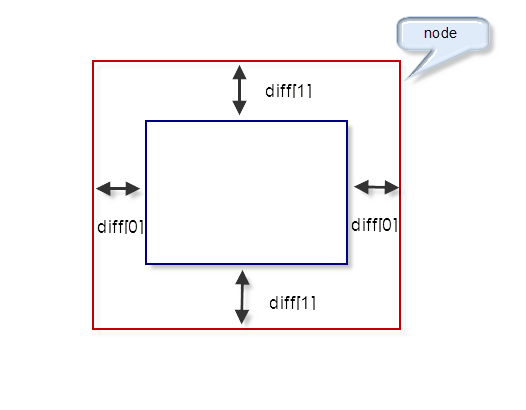
\includegraphics{scroll.png}

\end{fulllineitems}



\subparagraph{Methods Detail}
\label{api/component/dd/scroll:methods-detail}
\index{attach() (in module Scroll)}

\begin{fulllineitems}
\phantomsection\label{api/component/dd/scroll:Scroll.attach}\pysiglinewithargsret{\code{Scroll.}\bfcode{attach}}{}{}~
\begin{DUlineblock}{0em}
\item[] \textbf{attach} (drag)
\item[] 注册可拖放对象到当前容器.
\end{DUlineblock}
\begin{quote}\begin{description}
\item[{Parameters}] \leavevmode
\textbf{drag} ({\hyperref[api/component/dd/draggable:module-Draggable]{\emph{Draggable}}}) -- 需要使容器自动滚动的 Draggable 对象

\end{description}\end{quote}

\end{fulllineitems}


\index{unAttach() (in module Scroll)}

\begin{fulllineitems}
\phantomsection\label{api/component/dd/scroll:Scroll.unAttach}\pysiglinewithargsret{\code{Scroll.}\bfcode{unAttach}}{}{}~
\begin{DUlineblock}{0em}
\item[] \textbf{unAttach} (drag)
\item[] 解除当前容器关联的可拖放对象.
\end{DUlineblock}
\begin{quote}\begin{description}
\item[{Parameters}] \leavevmode
\textbf{drag} ({\hyperref[api/component/dd/draggable:module-Draggable]{\emph{Draggable}}}) -- 使容器自动滚动的 Draggable 对象

\end{description}\end{quote}

\end{fulllineitems}


\index{destroy() (in module Scroll)}

\begin{fulllineitems}
\phantomsection\label{api/component/dd/scroll:Scroll.destroy}\pysiglinewithargsret{\code{Scroll.}\bfcode{destroy}}{}{}~
\begin{DUlineblock}{0em}
\item[] \textbf{destroy} (drag)
\item[] 解除当前容器关联的所有可拖放对象.
\end{DUlineblock}

\end{fulllineitems}



\subsection{Switchable}
\label{api/component/switchable/index::doc}\label{api/component/switchable/index:switchable}
\begin{DUlineblock}{0em}
\item[] 该模块由 Switchable 基础类、插件和 Widget 类组成.
\item[] Switchable 基础类抽象了切换的基本操作, 通过插件机制实现了自动播放、循环、切换效果、延迟加载、倒计时动画等扩展功能, 最后封装成各个 Widget 类, 让用户能简明快速地调用.
\item[] 作者: \href{mailto:lifesinger@gmail.com}{玉伯}
\item[] \href{https://github.com/kissyteam/kissy/tree/master/src/switchable/}{源码} \textbar{} Demo
\end{DUlineblock}


\subsubsection{Classes in Switchable}
\label{api/component/switchable/index:classes-in-switchable}\phantomsection\label{api/component/switchable/switchable:module-Switchable}
\index{Switchable (module)}

\paragraph{Switchable}
\label{api/component/switchable/switchable::doc}\label{api/component/switchable/switchable:switchable}
\begin{DUlineblock}{0em}
\item[] Switchable 的核心类, S.Tabs/S.Slide/S.Accordion/S.Carousel 都是扩展自它.
\item[] 作者: \href{mailto:lifesinger@gmail.com}{玉伯}
\item[] \href{https://github.com/kissyteam/kissy/tree/master/src/switchable/}{源码} \textbar{} Demo
\end{DUlineblock}


\subparagraph{Class}
\label{api/component/switchable/switchable:class}\begin{itemize}
\item {}
{\hyperref[api/component/switchable/switchable:Switchable.Switchable]{\code{Switchable}}}

\end{itemize}


\subparagraph{Config Attributes}
\label{api/component/switchable/switchable:config-attributes}\begin{itemize}
\item {}
{\hyperref[api/component/switchable/switchable:Switchable.markupType]{\code{markupType}}}

\item {}
{\hyperref[api/component/switchable/switchable:Switchable.navCls]{\code{navCls}}}

\item {}
{\hyperref[api/component/switchable/switchable:Switchable.contentCls]{\code{contentCls}}}

\item {}
{\hyperref[api/component/switchable/switchable:Switchable.triggerCls]{\code{triggerCls}}}

\item {}
{\hyperref[api/component/switchable/switchable:Switchable.panelCls]{\code{panelCls}}}

\item {}
{\hyperref[api/component/switchable/switchable:Switchable.triggers]{\code{triggers}}}

\item {}
{\hyperref[api/component/switchable/switchable:Switchable.panels]{\code{panels}}}

\item {}
{\hyperref[api/component/switchable/switchable:Switchable.hasTriggers]{\code{hasTriggers}}}

\item {}
{\hyperref[api/component/switchable/switchable:Switchable.triggerType]{\code{triggerType}}}

\item {}
{\hyperref[api/component/switchable/switchable:Switchable.delay]{\code{delay}}}

\item {}
{\hyperref[api/component/switchable/switchable:Switchable.activeIndex]{\code{activeIndex}}}

\item {}
{\hyperref[api/component/switchable/switchable:Switchable.activeTriggerCls]{\code{activeTriggerCls}}}

\item {}
{\hyperref[api/component/switchable/switchable:Switchable.switchTo]{\code{switchTo}}}

\item {}
{\hyperref[api/component/switchable/switchable:Switchable.steps]{\code{steps}}}

\item {}
{\hyperref[api/component/switchable/switchable:Switchable.viewSize]{\code{viewSize}}}

\item {}
{\hyperref[api/component/switchable/switchable:Switchable.autoplay]{\code{autoplay}}}

\item {}
{\hyperref[api/component/switchable/switchable:Switchable.interval]{\code{interval}}}

\item {}
{\hyperref[api/component/switchable/switchable:Switchable.pauseOnHover]{\code{pauseOnHover}}}

\item {}
{\hyperref[api/component/switchable/switchable:Switchable.circular]{\code{circular}}}

\item {}
{\hyperref[api/component/switchable/switchable:Switchable.effect]{\code{effect}}}

\item {}
{\hyperref[api/component/switchable/switchable:Switchable.duration]{\code{duration}}}

\item {}
{\hyperref[api/component/switchable/switchable:Switchable.easing]{\code{easing}}}

\item {}
{\hyperref[api/component/switchable/switchable:Switchable.nativeAnim]{\code{nativeAnim}}}

\item {}
{\hyperref[api/component/switchable/switchable:Switchable.lazyDataType]{\code{lazyDataType}}}

\item {}
{\hyperref[api/component/switchable/switchable:Switchable.aria]{\code{aria}}}

\end{itemize}


\subparagraph{Properties}
\label{api/component/switchable/switchable:properties}\begin{itemize}
\item {}
{\hyperref[api/component/switchable/switchable:Switchable.container]{\code{container}}}

\item {}
{\hyperref[api/component/switchable/switchable:Switchable.config]{\code{config}}}

\item {}
{\hyperref[api/component/switchable/switchable:Switchable.triggers]{\code{triggers}}}

\item {}
{\hyperref[api/component/switchable/switchable:Switchable.panels]{\code{panels}}}

\item {}
{\hyperref[api/component/switchable/switchable:Switchable.content]{\code{content}}}

\item {}
{\hyperref[api/component/switchable/switchable:Switchable.length]{\code{length}}}

\item {}
{\hyperref[api/component/switchable/switchable:Switchable.activeIndex]{\code{activeIndex}}}

\item {}
{\hyperref[api/component/switchable/switchable:Switchable.switchTimer]{\code{switchTimer}}}

\end{itemize}


\subparagraph{Methods}
\label{api/component/switchable/switchable:methods}\begin{itemize}
\item {}
{\hyperref[api/component/switchable/switchable:Switchable.switchTo]{\code{switchTo()}}}

\item {}
{\hyperref[api/component/switchable/switchable:Switchable.prev]{\code{prev()}}}

\item {}
{\hyperref[api/component/switchable/switchable:Switchable.next]{\code{next()}}}

\end{itemize}


\subparagraph{Events}
\label{api/component/switchable/switchable:events}\begin{itemize}
\item {}
{\hyperref[api/component/switchable/switchable:Switchable.beforeSwitch]{\code{beforeSwitch()}}}

\item {}
{\hyperref[api/component/switchable/switchable:Switchable.switch]{\code{switch()}}}

\end{itemize}


\subparagraph{Class Detail}
\label{api/component/switchable/switchable:class-detail}
\index{Switchable (class in Switchable)}

\begin{fulllineitems}
\phantomsection\label{api/component/switchable/switchable:Switchable.Switchable}\pysigline{\strong{class }\code{Switchable.}\bfcode{Switchable}}{}~
\begin{DUlineblock}{0em}
\item[] \textbf{Switchable} (container{[}, config{]})
\end{DUlineblock}
\begin{quote}\begin{description}
\item[{Parameters}] \leavevmode\begin{itemize}
\item {}
\textbf{container} (\emph{String\textbar{}HTMLElement}) -- 容器

\item {}
\textbf{config} (\emph{object}) -- 可选, 配置项, 详细见下方 \textbf{Config Attributes Detail} .

\end{itemize}

\end{description}\end{quote}

\end{fulllineitems}



\subparagraph{Config Attributes Detail}
\label{api/component/switchable/switchable:config-attributes-detail}
\index{markupType (in module Switchable)}

\begin{fulllineitems}
\phantomsection\label{api/component/switchable/switchable:Switchable.markupType}\pysigline{\code{Switchable.}\bfcode{markupType}}{}
\{Number\} - 默认为0. 指明 DOM 结构标记的类型, 可取 0, 1, 2. 当取 0 时, 表示 DOM 是默认结构: 通过 nav 和 content 来获取 triggers 和 panels, 即通过配置以下两个参数获取.

\end{fulllineitems}


\index{navCls (in module Switchable)}

\begin{fulllineitems}
\phantomsection\label{api/component/switchable/switchable:Switchable.navCls}\pysigline{\code{Switchable.}\bfcode{navCls}}{}
\{String\} - triggers 所在容器的 class, 默认为 `ks-switchable-nav'.

\end{fulllineitems}


\index{contentCls (in module Switchable)}

\begin{fulllineitems}
\phantomsection\label{api/component/switchable/switchable:Switchable.contentCls}\pysigline{\code{Switchable.}\bfcode{contentCls}}{}
\{String\} - panels 所在容器的 class, 默认为 `ks-switchable-content'.

这种方式的 DOM 结构类似于:

\begin{Verbatim}[commandchars=\\\{\}]
\PYG{n+nt}{\textless{}div} \PYG{n+na}{id=}\PYG{l+s}{"J\PYGZus{}Slide"}\PYG{n+nt}{\textgreater{}}  \PYG{c}{\textless{}!--}\PYG{c}{ 容器元素 }\PYG{c}{--\textgreater{}}
    \PYG{n+nt}{\textless{}ul} \PYG{n+na}{class=}\PYG{l+s}{"ks-switchable-nav"}\PYG{n+nt}{\textgreater{}}  \PYG{c}{\textless{}!--}\PYG{c}{ 触发器列表 }\PYG{c}{--\textgreater{}}
        \PYG{n+nt}{\textless{}li} \PYG{n+na}{class=}\PYG{l+s}{"ks-active"}\PYG{n+nt}{\textgreater{}}标题 A\PYG{n+nt}{\textless{}/li\textgreater{}}
        \PYG{n+nt}{\textless{}li}\PYG{n+nt}{\textgreater{}}标题 B\PYG{n+nt}{\textless{}/li\textgreater{}}
        \PYG{n+nt}{\textless{}li}\PYG{n+nt}{\textgreater{}}标题 C\PYG{n+nt}{\textless{}/li\textgreater{}}
        \PYG{n+nt}{\textless{}li}\PYG{n+nt}{\textgreater{}}标题 D\PYG{n+nt}{\textless{}/li\textgreater{}}
    \PYG{n+nt}{\textless{}/ul\textgreater{}}
    \PYG{n+nt}{\textless{}div} \PYG{n+na}{class=}\PYG{l+s}{"ks-switchable-content"}\PYG{n+nt}{\textgreater{}}  \PYG{c}{\textless{}!--}\PYG{c}{ 面板列表 }\PYG{c}{--\textgreater{}}
        \PYG{n+nt}{\textless{}div}\PYG{n+nt}{\textgreater{}}内容 A\PYG{n+nt}{\textless{}/div\textgreater{}}
        \PYG{n+nt}{\textless{}div} \PYG{n+na}{style=}\PYG{l+s}{"display: none"}\PYG{n+nt}{\textgreater{}}内容 B\PYG{n+nt}{\textless{}/div\textgreater{}}
        \PYG{n+nt}{\textless{}div} \PYG{n+na}{style=}\PYG{l+s}{"display: none"}\PYG{n+nt}{\textgreater{}}内容 C\PYG{n+nt}{\textless{}/div\textgreater{}}
        \PYG{n+nt}{\textless{}div} \PYG{n+na}{style=}\PYG{l+s}{"display: none"}\PYG{n+nt}{\textgreater{}}内容 D\PYG{n+nt}{\textless{}/div\textgreater{}}
    \PYG{n+nt}{\textless{}/div\textgreater{}}
\PYG{n+nt}{\textless{}/div\textgreater{}}
\end{Verbatim}

当取 1 时,  表示 DOM 结构 可适度灵活:通过 cls 来获取 triggers 和 panels, 即通过配置以下两个参数获取.

\end{fulllineitems}


\index{triggerCls (in module Switchable)}

\begin{fulllineitems}
\phantomsection\label{api/component/switchable/switchable:Switchable.triggerCls}\pysigline{\code{Switchable.}\bfcode{triggerCls}}{}
\{String\} - 默认为 `ks-switchable-trigger', 会在 container 下寻找指定 class 的元素作为触发器.

\end{fulllineitems}


\index{panelCls (in module Switchable)}

\begin{fulllineitems}
\phantomsection\label{api/component/switchable/switchable:Switchable.panelCls}\pysigline{\code{Switchable.}\bfcode{panelCls}}{}
\{String\} - 默认为 `ks-switchable-panel', 会在 container 下寻找指定 class 的元素作为面板.

这种方式的 DOM 结构类似于:

\begin{Verbatim}[commandchars=\\\{\}]
\PYG{n+nt}{\textless{}div} \PYG{n+na}{id=}\PYG{l+s}{"J\PYGZus{}Accordion"}\PYG{n+nt}{\textgreater{}}
    \PYG{n+nt}{\textless{}div} \PYG{n+na}{class=}\PYG{l+s}{"ks-switchable-trigger ks-active"}\PYG{n+nt}{\textgreater{}}\PYG{n+nt}{\textless{}i} \PYG{n+na}{class=}\PYG{l+s}{"ks-icon"}\PYG{n+nt}{\textgreater{}}\PYG{n+nt}{\textless{}/i\textgreater{}}\PYG{n+nt}{\textless{}h3}\PYG{n+nt}{\textgreater{}}标题A\PYG{n+nt}{\textless{}/h3\textgreater{}}\PYG{n+nt}{\textless{}/div\textgreater{}}
    \PYG{n+nt}{\textless{}div} \PYG{n+na}{class=}\PYG{l+s}{"ks-switchable-panel"}\PYG{n+nt}{\textgreater{}}内容A\PYG{n+nt}{\textless{}br}\PYG{n+nt}{/\textgreater{}}内容A\PYG{n+nt}{\textless{}br}\PYG{n+nt}{/\textgreater{}}内容A\PYG{n+nt}{\textless{}/div\textgreater{}}
    \PYG{n+nt}{\textless{}div} \PYG{n+na}{class=}\PYG{l+s}{"ks-switchable-trigger"}\PYG{n+nt}{\textgreater{}}\PYG{n+nt}{\textless{}i} \PYG{n+na}{class=}\PYG{l+s}{"ks-icon"}\PYG{n+nt}{\textgreater{}}\PYG{n+nt}{\textless{}/i\textgreater{}}\PYG{n+nt}{\textless{}h3}\PYG{n+nt}{\textgreater{}}标题B\PYG{n+nt}{\textless{}/h3\textgreater{}}\PYG{n+nt}{\textless{}/div\textgreater{}}
    \PYG{n+nt}{\textless{}div} \PYG{n+na}{class=}\PYG{l+s}{"ks-switchable-panel"} \PYG{n+na}{style=}\PYG{l+s}{"display:none;"}\PYG{n+nt}{\textgreater{}}内容B\PYG{n+nt}{\textless{}br}\PYG{n+nt}{/\textgreater{}}内容B\PYG{n+nt}{\textless{}br}\PYG{n+nt}{/\textgreater{}}内容B\PYG{n+nt}{\textless{}/div\textgreater{}}
    \PYG{n+nt}{\textless{}div} \PYG{n+na}{class=}\PYG{l+s}{"ks-switchable-trigger"}\PYG{n+nt}{\textgreater{}}\PYG{n+nt}{\textless{}i} \PYG{n+na}{class=}\PYG{l+s}{"ks-icon"}\PYG{n+nt}{\textgreater{}}\PYG{n+nt}{\textless{}/i\textgreater{}}\PYG{n+nt}{\textless{}h3}\PYG{n+nt}{\textgreater{}}标题C\PYG{n+nt}{\textless{}/h3\textgreater{}}\PYG{n+nt}{\textless{}/div\textgreater{}}
    \PYG{n+nt}{\textless{}div} \PYG{n+na}{class=}\PYG{l+s}{"ks-switchable-panel"} \PYG{n+na}{style=}\PYG{l+s}{"display:none;"}\PYG{n+nt}{\textgreater{}}内容C\PYG{n+nt}{\textless{}br}\PYG{n+nt}{/\textgreater{}}内容C\PYG{n+nt}{\textless{}br}\PYG{n+nt}{/\textgreater{}}内容C\PYG{n+nt}{\textless{}br}\PYG{n+nt}{/\textgreater{}}内容C\PYG{n+nt}{\textless{}br}\PYG{n+nt}{/\textgreater{}}内容C\PYG{n+nt}{\textless{}/div\textgreater{}}
    \PYG{n+nt}{\textless{}div} \PYG{n+na}{class=}\PYG{l+s}{"ks-switchable-trigger last-trigger"}\PYG{n+nt}{\textgreater{}}\PYG{n+nt}{\textless{}i} \PYG{n+na}{class=}\PYG{l+s}{"ks-icon"}\PYG{n+nt}{\textgreater{}}\PYG{n+nt}{\textless{}/i\textgreater{}}\PYG{n+nt}{\textless{}h3}\PYG{n+nt}{\textgreater{}}标题D\PYG{n+nt}{\textless{}/h3\textgreater{}}\PYG{n+nt}{\textless{}/div\textgreater{}}
    \PYG{n+nt}{\textless{}div} \PYG{n+na}{class=}\PYG{l+s}{"ks-switchable-panel last-panel"} \PYG{n+na}{style=}\PYG{l+s}{"display:none;"}\PYG{n+nt}{\textgreater{}}内容D\PYG{n+nt}{\textless{}br}\PYG{n+nt}{/\textgreater{}}内容D\PYG{n+nt}{\textless{}br}\PYG{n+nt}{/\textgreater{}}内容D\PYG{n+nt}{\textless{}/div\textgreater{}}
\PYG{n+nt}{\textless{}/div\textgreater{}}
\end{Verbatim}

当取 2 时,  表示 DOM 结构 完全自由: 直接传入 triggers 和 panels, 即通过配置以下两个参数获取. 这种方式下, DOM 结构就非常自由了, 传入什么内容有你自己定, 只需要 triggers 和 panels 的数量保持一致就好.

\end{fulllineitems}


\index{triggers (in module Switchable)}

\begin{fulllineitems}
\phantomsection\label{api/component/switchable/switchable:Switchable.triggers}\pysigline{\code{Switchable.}\bfcode{triggers}}{}
\{Array\textless{}HTMLElement\textgreater{}\} - 默认为 {[}{]}, 触发器数组.

\end{fulllineitems}


\index{panels (in module Switchable)}

\begin{fulllineitems}
\phantomsection\label{api/component/switchable/switchable:Switchable.panels}\pysigline{\code{Switchable.}\bfcode{panels}}{}
\{Array\textless{}HTMLElement\textgreater{}\} - 默认为 {[}{]}, 面板数组.

\end{fulllineitems}


\index{hasTriggers (in module Switchable)}

\begin{fulllineitems}
\phantomsection\label{api/component/switchable/switchable:Switchable.hasTriggers}\pysigline{\code{Switchable.}\bfcode{hasTriggers}}{}
\{Boolean\} - 默认为 true, 是否有触点.

\end{fulllineitems}


\index{triggerType (in module Switchable)}

\begin{fulllineitems}
\phantomsection\label{api/component/switchable/switchable:Switchable.triggerType}\pysigline{\code{Switchable.}\bfcode{triggerType}}{}
\{String\} - 默认为 `mouse' , 触发类型,  可选为'mouse' 或 `click'.

\end{fulllineitems}


\index{delay (in module Switchable)}

\begin{fulllineitems}
\phantomsection\label{api/component/switchable/switchable:Switchable.delay}\pysigline{\code{Switchable.}\bfcode{delay}}{}
\{Number\} - 默认为 .1 , 触发延迟时间, 单位为s.

\end{fulllineitems}


\index{activeIndex (in module Switchable)}

\begin{fulllineitems}
\phantomsection\label{api/component/switchable/switchable:Switchable.activeIndex}\pysigline{\code{Switchable.}\bfcode{activeIndex}}{}
\{Number\} - 默认为 0,  markup 的默认激活项, 应该与此 index 一致.

\begin{notice}{note}{Note:}
使用此项时, 需要让激活项对应的 trigger 和 panel 的 HTMLElement, 在 DOM 结构上设置为 激活状态, 不然无法正确切换
\end{notice}

\end{fulllineitems}


\index{activeTriggerCls (in module Switchable)}

\begin{fulllineitems}
\phantomsection\label{api/component/switchable/switchable:Switchable.activeTriggerCls}\pysigline{\code{Switchable.}\bfcode{activeTriggerCls}}{}
\{String\} - 激活某个 trigger 时设置的 class , 默认是 `ks-active'.

\end{fulllineitems}


\index{switchTo (in module Switchable)}

\begin{fulllineitems}
\phantomsection\label{api/component/switchable/switchable:Switchable.switchTo}\pysigline{\code{Switchable.}\bfcode{switchTo}}{}
\{Number\} - 初始话时, 自动切换到指定面板, 默认为 0 , 即第一个.

\begin{notice}{note}{Note:}
switchTo 和 activeIndex 的区别是:
\begin{itemize}
\item {}
activeIndex 需要 DOM 上设置激活状态, 初始化后不会去切换状态;

\item {}
switchTo 则不需要修改 DOM, 但 switchTo 设置后, 会去切换到指定状态, 这在用了一些动画效果时, 切换动作更为明显;

\end{itemize}
\end{notice}

\end{fulllineitems}


\index{steps (in module Switchable)}

\begin{fulllineitems}
\phantomsection\label{api/component/switchable/switchable:Switchable.steps}\pysigline{\code{Switchable.}\bfcode{steps}}{}
\{Number\} - 步长, 表示每次切换要间隔多少个 panels, 默认为 1.

\end{fulllineitems}


\index{viewSize (in module Switchable)}

\begin{fulllineitems}
\phantomsection\label{api/component/switchable/switchable:Switchable.viewSize}\pysigline{\code{Switchable.}\bfcode{viewSize}}{}
\{Array\} - 可见视图区域的大小. 一般不需要设定此值, 仅当获取值不正确时, 用于手工指定大小, 默认为 {[}{]}.

\end{fulllineitems}


\index{autoplay (in module Switchable)}

\begin{fulllineitems}
\phantomsection\label{api/component/switchable/switchable:Switchable.autoplay}\pysigline{\code{Switchable.}\bfcode{autoplay}}{}
\{Boolean\} - 是否自动切换, 默认为 false, 开启后, 不需要触发触发器, 即可自动播放.

\end{fulllineitems}


\index{interval (in module Switchable)}

\begin{fulllineitems}
\phantomsection\label{api/component/switchable/switchable:Switchable.interval}\pysigline{\code{Switchable.}\bfcode{interval}}{}
\{Number\} - 自动播放间隔时间, 以 s 为单位, 默认为 5.

\end{fulllineitems}


\index{pauseOnHover (in module Switchable)}

\begin{fulllineitems}
\phantomsection\label{api/component/switchable/switchable:Switchable.pauseOnHover}\pysigline{\code{Switchable.}\bfcode{pauseOnHover}}{}
\{Boolean\} - triggerType 为 mouse 时, 鼠标悬停在 slide 上是否暂停自动播放, 默认为 true.

\end{fulllineitems}


\index{circular (in module Switchable)}

\begin{fulllineitems}
\phantomsection\label{api/component/switchable/switchable:Switchable.circular}\pysigline{\code{Switchable.}\bfcode{circular}}{}
\{Boolean\} - 是否循环切换, 默认为 false, 是否循环播放, 当切换到最初/最后一个时, 是否切换到最后/最初一个.

\end{fulllineitems}


\index{effect (in module Switchable)}

\begin{fulllineitems}
\phantomsection\label{api/component/switchable/switchable:Switchable.effect}\pysigline{\code{Switchable.}\bfcode{effect}}{}
\{String\} - 动画效果函数, 默认没有特效, 可取 \code{scrollx}, \code{scrolly}, \code{fade} 或者直接传入自定义效果函数.

\end{fulllineitems}


\index{duration (in module Switchable)}

\begin{fulllineitems}
\phantomsection\label{api/component/switchable/switchable:Switchable.duration}\pysigline{\code{Switchable.}\bfcode{duration}}{}
\{Number\} - 默认为 .5, 动画的时长.

\end{fulllineitems}


\index{easing (in module Switchable)}

\begin{fulllineitems}
\phantomsection\label{api/component/switchable/switchable:Switchable.easing}\pysigline{\code{Switchable.}\bfcode{easing}}{}
\{String\textbar{}Function\} - 动画效果, 详见 {\hyperref[api/core/anim/index:module-Anim]{\code{Anim}}}, 默认为 \code{easeNone} .

\end{fulllineitems}


\index{nativeAnim (in module Switchable)}

\begin{fulllineitems}
\phantomsection\label{api/component/switchable/switchable:Switchable.nativeAnim}\pysigline{\code{Switchable.}\bfcode{nativeAnim}}{}
\{Boolean\} - 是否优先使用原生 css3 transition, 默认为 \code{true}, 同 {\hyperref[api/core/anim/index:module-Anim]{\code{Anim}}} 中的  \emph{nativeSupport} 参数  .

\end{fulllineitems}


\index{lazyDataType (in module Switchable)}

\begin{fulllineitems}
\phantomsection\label{api/component/switchable/switchable:Switchable.lazyDataType}\pysigline{\code{Switchable.}\bfcode{lazyDataType}}{}
\{String\} - 默认为 `area-data', 设置延迟加载时使用的数据类型, 可取 \code{area-data}, 即 \code{textarea} 标签 或 \code{img-src}, 即 \code{img} 标签.

\begin{notice}{note}{Note:}
支持懒加载, 需要载入 S.Datalazyload, 详见 {\hyperref[api/component/datalazyload/index:DataLazyload.DataLazyload]{\code{DataLazyload}}}
\end{notice}

\end{fulllineitems}


\index{aria (in module Switchable)}

\begin{fulllineitems}
\phantomsection\label{api/component/switchable/switchable:Switchable.aria}\pysigline{\code{Switchable.}\bfcode{aria}}{}
\{Boolean\} - 无障碍访问支持, 默认为 false, 即关闭.

\end{fulllineitems}



\subparagraph{Properties Detail}
\label{api/component/switchable/switchable:properties-detail}
\index{container (in module Switchable)}

\begin{fulllineitems}
\phantomsection\label{api/component/switchable/switchable:Switchable.container}\pysigline{\code{Switchable.}\bfcode{container}}{}
\{HTMLElement\} - 只读, 容器元素

\end{fulllineitems}


\index{config (in module Switchable)}

\begin{fulllineitems}
\phantomsection\label{api/component/switchable/switchable:Switchable.config}\pysigline{\code{Switchable.}\bfcode{config}}{}
\{Object\} - - 只读, 配置信息

\end{fulllineitems}


\index{triggers (in module Switchable)}

\begin{fulllineitems}
\pysigline{\code{Switchable.}\bfcode{triggers}}{}
\{Array\} - 只读, 触发器集合, 可以为空值 {[}{]}

\end{fulllineitems}


\index{panels (in module Switchable)}

\begin{fulllineitems}
\pysigline{\code{Switchable.}\bfcode{panels}}{}
\{Array\} - 只读, 切换面板集合,  可以为空值 {[}{]}

\end{fulllineitems}


\index{content (in module Switchable)}

\begin{fulllineitems}
\phantomsection\label{api/component/switchable/switchable:Switchable.content}\pysigline{\code{Switchable.}\bfcode{content}}{}
\{HTMLElement\} - 只读, 存放面板的容器元素

\end{fulllineitems}


\index{length (in module Switchable)}

\begin{fulllineitems}
\phantomsection\label{api/component/switchable/switchable:Switchable.length}\pysigline{\code{Switchable.}\bfcode{length}}{}
\{Number\} - 只读, 触发器或面板的个数

\end{fulllineitems}


\index{activeIndex (in module Switchable)}

\begin{fulllineitems}
\pysigline{\code{Switchable.}\bfcode{activeIndex}}{}
\{Number\} - 只读, 当前被激活的触发器序号, 从0 开始

\end{fulllineitems}


\index{switchTimer (in module Switchable)}

\begin{fulllineitems}
\phantomsection\label{api/component/switchable/switchable:Switchable.switchTimer}\pysigline{\code{Switchable.}\bfcode{switchTimer}}{}
\{Object\} - 只读, 切换定时器, 一般作为内部使用

\end{fulllineitems}



\subparagraph{Methods Detail}
\label{api/component/switchable/switchable:methods-detail}
\index{switchTo() (in module Switchable)}

\begin{fulllineitems}
\pysiglinewithargsret{\code{Switchable.}\bfcode{switchTo}}{}{}~
\begin{DUlineblock}{0em}
\item[] \textbf{switchTo} (index, direction, ev, callback)
\item[] 切换到某个视图
\end{DUlineblock}
\begin{quote}\begin{description}
\item[{Parameters}] \leavevmode\begin{itemize}
\item {}
\textbf{index} (\emph{Number}) -- 要切换的项

\item {}
\textbf{direction} (\emph{String}) -- (可选) 方向, 用于 effect, 可取 `forward', `backward', 或者不设置

\item {}
\textbf{ev} (\emph{EventObject}) -- (可选) 引起该操作的事件

\item {}
\textbf{callback} (\emph{Function}) -- (可选) 运行完回调, 和绑定 switch 事件作用一样

\end{itemize}

\end{description}\end{quote}

\end{fulllineitems}


\index{prev() (in module Switchable)}

\begin{fulllineitems}
\phantomsection\label{api/component/switchable/switchable:Switchable.prev}\pysiglinewithargsret{\code{Switchable.}\bfcode{prev}}{}{}~
\begin{DUlineblock}{0em}
\item[] \textbf{prev} ({[}ev{]})
\item[] 切换到上一视图
\end{DUlineblock}
\begin{quote}\begin{description}
\item[{Parameters}] \leavevmode
\textbf{ev} (\emph{EventObject}) -- 引起该操作的事件

\end{description}\end{quote}

\end{fulllineitems}


\index{next() (in module Switchable)}

\begin{fulllineitems}
\phantomsection\label{api/component/switchable/switchable:Switchable.next}\pysiglinewithargsret{\code{Switchable.}\bfcode{next}}{}{}~
\begin{DUlineblock}{0em}
\item[] \textbf{next} (ev)
\item[] 切换到下一视图
\end{DUlineblock}
\begin{quote}\begin{description}
\item[{Parameters}] \leavevmode
\textbf{ev} (\emph{EventObject}) -- (可选) 引起该操作的事件

\end{description}\end{quote}

\end{fulllineitems}



\subparagraph{Events Detail}
\label{api/component/switchable/switchable:events-detail}
\index{beforeSwitch() (in module Switchable)}

\begin{fulllineitems}
\phantomsection\label{api/component/switchable/switchable:Switchable.beforeSwitch}\pysiglinewithargsret{\code{Switchable.}\bfcode{beforeSwitch}}{}{}~
\begin{DUlineblock}{0em}
\item[] \textbf{beforeSwitch} (ev)
\item[] 切换前触发. 当该事件的函数处理器返回 false, 则会阻止切换动作.
\end{DUlineblock}
\begin{quote}\begin{description}
\item[{Parameters}] \leavevmode\begin{itemize}
\item {}
\textbf{ev} (\emph{Object}) -- 事件对象

\item {}
\textbf{ev.toIndex} (\emph{Number}) -- 即将切换到的tab的索引号

\end{itemize}

\end{description}\end{quote}

\end{fulllineitems}


\index{switch() (in module Switchable)}

\begin{fulllineitems}
\phantomsection\label{api/component/switchable/switchable:Switchable.switch}\pysiglinewithargsret{\code{Switchable.}\bfcode{switch}}{}{}~
\begin{DUlineblock}{0em}
\item[] \textbf{switch} (ev)
\item[] 切换后触发.
\end{DUlineblock}
\begin{quote}\begin{description}
\item[{Parameters}] \leavevmode\begin{itemize}
\item {}
\textbf{ev} (\emph{Object}) -- 事件对象

\item {}
\textbf{ev.currentIndex} (\emph{Number}) -- 当前切换到的tab的索引号

\end{itemize}

\end{description}\end{quote}

\end{fulllineitems}

\phantomsection\label{api/component/switchable/tabs:module-Tabs}
\index{Tabs (module)}

\paragraph{Tabs}
\label{api/component/switchable/tabs:tabs}\label{api/component/switchable/tabs::doc}
\begin{DUlineblock}{0em}
\item[] 卡盘
\item[] 作者: \href{mailto:lifesinger@gmail.com}{玉伯}
\item[] \href{https://github.com/kissyteam/kissy/tree/master/src/switchable/tabs/}{源码} \textbar{} Demo
\item[] Tabs 接口及配置项, 与 {\hyperref[api/component/switchable/switchable:module-Switchable]{\code{Switchable}}} 完全相同.
\end{DUlineblock}
\phantomsection\label{api/component/switchable/slide:module-Slide}
\index{Slide (module)}

\paragraph{Slide}
\label{api/component/switchable/slide:slide}\label{api/component/switchable/slide::doc}
\begin{DUlineblock}{0em}
\item[] Slide
\item[] 作者: \href{mailto:lifesinger@gmail.com}{玉伯}
\item[] \href{https://github.com/kissyteam/kissy/tree/master/src/switchable/accordion/slide/}{源码} \textbar{} Demo
\end{DUlineblock}


\subparagraph{Config Attributes Detail}
\label{api/component/switchable/slide:config-attributes-detail}\begin{quote}

Slide 接口及配置项, 与 {\hyperref[api/component/switchable/switchable:module-Switchable]{\code{Switchable}}} 相同, 其中以下配置项的默认值有所区别:

\index{autoplay (in module Slide)}

\begin{fulllineitems}
\phantomsection\label{api/component/switchable/slide:Slide.autoplay}\pysigline{\code{Slide.}\bfcode{autoplay}}{}
\{Boolean\} - 默认为true, 是否自动切换.

\end{fulllineitems}


\index{circular (in module Slide)}

\begin{fulllineitems}
\phantomsection\label{api/component/switchable/slide:Slide.circular}\pysigline{\code{Slide.}\bfcode{circular}}{}
\{Boolean\} - 默认为true, 是否循环切换.

\end{fulllineitems}

\end{quote}
\phantomsection\label{api/component/switchable/carousel:module-Carousel}
\index{Carousel (module)}

\paragraph{Carousel}
\label{api/component/switchable/carousel::doc}\label{api/component/switchable/carousel:carousel}
\begin{DUlineblock}{0em}
\item[] Carousel
\item[] 作者: \href{mailto:lifesinger@gmail.com}{玉伯}
\item[] \href{https://github.com/kissyteam/kissy/tree/master/src/switchable/carousel/}{源码} \textbar{} Demo
\end{DUlineblock}


\subparagraph{Config Attributes Detail}
\label{api/component/switchable/carousel:config-attributes-detail}\begin{quote}

Carousel 接口及配置项, 与 {\hyperref[api/component/switchable/switchable:module-Switchable]{\code{Switchable}}} 相同, 其中以下配置项的默认值有所区别:

\index{circular (in module Carousel)}

\begin{fulllineitems}
\phantomsection\label{api/component/switchable/carousel:Carousel.circular}\pysigline{\code{Carousel.}\bfcode{circular}}{}
\{Boolean\} - 默认为true, 是否循环切换.

\end{fulllineitems}


\index{prevBtnCls (in module Carousel)}

\begin{fulllineitems}
\phantomsection\label{api/component/switchable/carousel:Carousel.prevBtnCls}\pysigline{\code{Carousel.}\bfcode{prevBtnCls}}{}
\{String\} - 默认为 `ks-switchable-prev-btn', 前一个触发器的 cls.

\end{fulllineitems}


\index{nextBtnCls (in module Carousel)}

\begin{fulllineitems}
\phantomsection\label{api/component/switchable/carousel:Carousel.nextBtnCls}\pysigline{\code{Carousel.}\bfcode{nextBtnCls}}{}
\{String\} - 默认为 `ks-switchable-next-btn', 后一个触发器的 cls.

\end{fulllineitems}


\index{disableBtnCls (in module Carousel)}

\begin{fulllineitems}
\phantomsection\label{api/component/switchable/carousel:Carousel.disableBtnCls}\pysigline{\code{Carousel.}\bfcode{disableBtnCls}}{}
\{String\} - 默认为 `ks-switchable-disable-btn', 触发器不可用时的 cls.

\end{fulllineitems}

\end{quote}
\phantomsection\label{api/component/switchable/accordion:module-Accordion}
\index{Accordion (module)}

\paragraph{Accordion}
\label{api/component/switchable/accordion::doc}\label{api/component/switchable/accordion:accordion}
\begin{DUlineblock}{0em}
\item[] 手风琴
\item[] 作者: \href{mailto:fool2fish@gmail.com}{fool2fish}
\item[] \href{https://github.com/kissyteam/kissy/tree/master/src/switchable/accordion/}{源码} \textbar{} Demo
\end{DUlineblock}


\subparagraph{Config Attributes Detail}
\label{api/component/switchable/accordion:config-attributes-detail}\begin{quote}

Carousel 接口及配置项, 与 {\hyperref[api/component/switchable/switchable:module-Switchable]{\code{Switchable}}} 相同, 其中以下配置项的默认值有所区别:

\index{markupType (in module Accordion)}

\begin{fulllineitems}
\phantomsection\label{api/component/switchable/accordion:Accordion.markupType}\pysigline{\code{Accordion.}\bfcode{markupType}}{}
\{Number\} - 默认为 1 , 选择自定义 trigger 和 panel 的 class.

\end{fulllineitems}


\index{triggerType (in module Accordion)}

\begin{fulllineitems}
\phantomsection\label{api/component/switchable/accordion:Accordion.triggerType}\pysigline{\code{Accordion.}\bfcode{triggerType}}{}
\{Boolean\} - `click' , 点击触发.

\end{fulllineitems}


\index{multiple (in module Accordion)}

\begin{fulllineitems}
\phantomsection\label{api/component/switchable/accordion:Accordion.multiple}\pysigline{\code{Accordion.}\bfcode{multiple}}{}
\{Boolean\} - 默认为 false, 是否开启同时展开多个面板功能.

\end{fulllineitems}

\end{quote}
\phantomsection\label{api/component/suggest/index:module-Suggest}
\index{Suggest (module)}

\subsection{Suggest}
\label{api/component/suggest/index:suggest}\label{api/component/suggest/index::doc}
\begin{DUlineblock}{0em}
\item[] 提示补全, 支持如下功能:
\item[]
\begin{DUlineblock}{\DUlineblockindent}
\item[] - 完全跨域
\item[] - cache 功能
\item[] - 支持键盘控制:上下选择及回车后直接提交, ESC 键关闭
\item[] - 支持鼠标控制:鼠标选择和点击提交功能
\item[] - 支持匹配文字加亮
\item[] - 动画效果
\item[] - 在提示层中显示第一个搜索结果
\item[] - 整合本地表单的提示记录
\item[] - 关键词的模糊匹配提示功能
\item[] - 自定义提示Dom渲染
\item[] - 支持本地数据
\end{DUlineblock}
\item[] 作者: \href{mailto:lifesinger@gmail.com}{玉伯}
\item[] \href{https://github.com/kissyteam/kissy/tree/master/src/suggest}{源码} \textbar{} Demo
\end{DUlineblock}


\subsubsection{Class}
\label{api/component/suggest/index:class}\begin{itemize}
\item {}
{\hyperref[api/component/suggest/index:Suggest.Suggest]{\code{Suggest}}}

\end{itemize}


\subsubsection{Config Attributes}
\label{api/component/suggest/index:config-attributes}\begin{itemize}
\item {}
{\hyperref[api/component/suggest/index:Suggest.containerCls]{\code{containerCls}}}

\item {}
{\hyperref[api/component/suggest/index:Suggest.containerWidth]{\code{containerWidth}}}

\item {}
{\hyperref[api/component/suggest/index:Suggest.resultFormat]{\code{resultFormat}}}

\item {}
{\hyperref[api/component/suggest/index:Suggest.closeBtn]{\code{closeBtn}}}

\item {}
{\hyperref[api/component/suggest/index:Suggest.closeBtnText]{\code{closeBtnText}}}

\item {}
{\hyperref[api/component/suggest/index:Suggest.shim]{\code{shim}}}

\item {}
{\hyperref[api/component/suggest/index:Suggest.autoFocus]{\code{autoFocus}}}

\item {}
{\hyperref[api/component/suggest/index:Suggest.submitOnSelect]{\code{submitOnSelect}}}

\item {}
{\hyperref[api/component/suggest/index:Suggest.offset]{\code{offset}}}

\item {}
{\hyperref[api/component/suggest/index:Suggest.charset]{\code{charset}}}

\item {}
{\hyperref[api/component/suggest/index:Suggest.callbackName]{\code{callbackName}}}

\item {}
{\hyperref[api/component/suggest/index:Suggest.callbackFn]{\code{callbackFn}}}

\item {}
{\hyperref[api/component/suggest/index:Suggest.queryName]{\code{queryName}}}

\item {}
{\hyperref[api/component/suggest/index:Suggest.dataType]{\code{dataType}}}

\item {}
{\hyperref[api/component/suggest/index:Suggest.contentRender]{\code{contentRender}}}

\end{itemize}


\subsubsection{Properties}
\label{api/component/suggest/index:properties}\begin{itemize}
\item {}
{\hyperref[api/component/suggest/index:Suggest.textInput]{\code{textInput}}}

\item {}
{\hyperref[api/component/suggest/index:Suggest.config]{\code{config}}}

\item {}
{\hyperref[api/component/suggest/index:Suggest.dataSource]{\code{dataSource}}}

\item {}
{\hyperref[api/component/suggest/index:Suggest.returnedData]{\code{returnedData}}}

\item {}
{\hyperref[api/component/suggest/index:Suggest.container]{\code{container}}}

\item {}
{\hyperref[api/component/suggest/index:Suggest.content]{\code{content}}}

\item {}
{\hyperref[api/component/suggest/index:Suggest.footer]{\code{footer}}}

\item {}
{\hyperref[api/component/suggest/index:Suggest.query]{\code{query}}}

\item {}
{\hyperref[api/component/suggest/index:Suggest.queryParams]{\code{queryParams}}}

\item {}
{\hyperref[api/component/suggest/index:Suggest.dataScript]{\code{dataScript}}}

\item {}
{\hyperref[api/component/suggest/index:Suggest.selectedItem]{\code{selectedItem}}}

\end{itemize}


\subsubsection{Methods}
\label{api/component/suggest/index:methods}\begin{itemize}
\item {}
{\hyperref[api/component/suggest/index:Suggest.start]{\code{start()}}}

\item {}
{\hyperref[api/component/suggest/index:Suggest.stop]{\code{stop()}}}

\item {}
{\hyperref[api/component/suggest/index:Suggest.show]{\code{show()}}}

\item {}
{\hyperref[api/component/suggest/index:Suggest.hide]{\code{hide()}}}

\item {}
{\hyperref[api/component/suggest/index:Suggest.isVisible]{\code{isVisible()}}}

\end{itemize}


\subsubsection{Events}
\label{api/component/suggest/index:events}\begin{itemize}
\item {}
{\hyperref[api/component/suggest/index:Suggest.beforeStart]{\code{beforeStart()}}}

\item {}
{\hyperref[api/component/suggest/index:Suggest.itemSelect]{\code{itemSelect()}}}

\item {}
{\hyperref[api/component/suggest/index:Suggest.beforeSubmit]{\code{beforeSubmit()}}}

\item {}
{\hyperref[api/component/suggest/index:Suggest.beforeDataRequest]{\code{beforeDataRequest()}}}

\item {}
{\hyperref[api/component/suggest/index:Suggest.dataReturn]{\code{dataReturn()}}}

\item {}
{\hyperref[api/component/suggest/index:Suggest.updateFooter]{\code{updateFooter()}}}

\item {}
{\hyperref[api/component/suggest/index:Suggest.beforeShow]{\code{beforeShow()}}}

\end{itemize}


\subsubsection{Class Detail}
\label{api/component/suggest/index:class-detail}
\index{Suggest (class in Suggest)}

\begin{fulllineitems}
\phantomsection\label{api/component/suggest/index:Suggest.Suggest}\pysigline{\strong{class }\code{Suggest.}\bfcode{Suggest}}{}~
\begin{DUlineblock}{0em}
\item[] \textbf{Suggest} (textInput, dataSource{[}, config{]})
\end{DUlineblock}
\begin{quote}\begin{description}
\item[{Parameters}] \leavevmode\begin{itemize}
\item {}
\textbf{textInput} (\emph{String\textbar{}HTMLElement}) -- 输入框.

\item {}
\textbf{dataSource} (\emph{String\textbar{}Array\textless{}Object\textgreater{}}) -- 获取提示的数据源, 可为远程URL, 或本地数据.

\item {}
\textbf{config} (\emph{Object}) -- 配置项, 详细见下方 \textbf{Config Attributes Detail} .

\end{itemize}

\end{description}\end{quote}

提示层的默认HTML结构如下:

\begin{Verbatim}[commandchars=\\\{\}]
\PYG{n+nt}{\textless{}div} \PYG{n+na}{class=}\PYG{l+s}{'ks-suggest-container \PYGZob{}containerCls\PYGZcb{}'}\PYG{n+nt}{\textgreater{}}
    \PYG{n+nt}{\textless{}ol} \PYG{n+na}{class=}\PYG{l+s}{"ks-suggest-content"}\PYG{n+nt}{\textgreater{}}
        \PYG{n+nt}{\textless{}li}\PYG{n+nt}{\textgreater{}}
            \PYG{n+nt}{\textless{}span} \PYG{n+na}{class=}\PYG{l+s}{'ks-suggest-key'}\PYG{n+nt}{\textgreater{}}...\PYG{n+nt}{\textless{}/span\textgreater{}}
            \PYG{n+nt}{\textless{}span} \PYG{n+na}{class=}\PYG{l+s}{'ks-suggest-result'}\PYG{n+nt}{\textgreater{}}...\PYG{n+nt}{\textless{}/span\textgreater{}}
        \PYG{n+nt}{\textless{}/li\textgreater{}}
    \PYG{n+nt}{\textless{}/ol\textgreater{}}
    \PYG{n+nt}{\textless{}div} \PYG{n+na}{class=}\PYG{l+s}{'ks-suggest-footer'}\PYG{n+nt}{\textgreater{}}
        \PYG{n+nt}{\textless{}a} \PYG{n+na}{class=}\PYG{l+s}{'ks-suggest-close-btn'}\PYG{n+nt}{\textgreater{}}...\PYG{n+nt}{\textless{}/a\textgreater{}}
    \PYG{n+nt}{\textless{}/div\textgreater{}}
\PYG{n+nt}{\textless{}/div\textgreater{}}
\end{Verbatim}

\end{fulllineitems}



\subsubsection{Config Attributes Detail}
\label{api/component/suggest/index:config-attributes-detail}
\index{containerCls (in module Suggest)}

\begin{fulllineitems}
\phantomsection\label{api/component/suggest/index:Suggest.containerCls}\pysigline{\code{Suggest.}\bfcode{containerCls}}{}
\{String\} - 用户附加给悬浮提示层的 class.

\end{fulllineitems}


\index{containerWidth (in module Suggest)}

\begin{fulllineitems}
\phantomsection\label{api/component/suggest/index:Suggest.containerWidth}\pysigline{\code{Suggest.}\bfcode{containerWidth}}{}
\{String\} - 默认为和input等宽. 提示层的宽度, 必须带单位, 如`200px', `10\%' 等.

\end{fulllineitems}


\index{resultFormat (in module Suggest)}

\begin{fulllineitems}
\phantomsection\label{api/component/suggest/index:Suggest.resultFormat}\pysigline{\code{Suggest.}\bfcode{resultFormat}}{}
\{String\} - 默认为 `\%result\%' ,  result 的格式.

\end{fulllineitems}


\index{closeBtn (in module Suggest)}

\begin{fulllineitems}
\phantomsection\label{api/component/suggest/index:Suggest.closeBtn}\pysigline{\code{Suggest.}\bfcode{closeBtn}}{}
\{Boolean\} - 默认为 false, 是否显示关闭按钮.

\end{fulllineitems}


\index{closeBtnText (in module Suggest)}

\begin{fulllineitems}
\phantomsection\label{api/component/suggest/index:Suggest.closeBtnText}\pysigline{\code{Suggest.}\bfcode{closeBtnText}}{}
\{String\} - 默认为 `关闭', 关闭按钮上的文字.

\end{fulllineitems}


\index{shim (in module Suggest)}

\begin{fulllineitems}
\phantomsection\label{api/component/suggest/index:Suggest.shim}\pysigline{\code{Suggest.}\bfcode{shim}}{}
\{Boolean\} - 是否需要 iframe shim 默认只在 ie6 下显示.

\end{fulllineitems}


\index{autoFocus (in module Suggest)}

\begin{fulllineitems}
\phantomsection\label{api/component/suggest/index:Suggest.autoFocus}\pysigline{\code{Suggest.}\bfcode{autoFocus}}{}
\{Boolean\} - 默认为 false , 初始化后, 自动激活.

\end{fulllineitems}


\index{submitOnSelect (in module Suggest)}

\begin{fulllineitems}
\phantomsection\label{api/component/suggest/index:Suggest.submitOnSelect}\pysigline{\code{Suggest.}\bfcode{submitOnSelect}}{}
\{Boolean\} - 默认为 true , 选择某项时, 是否自动提交表单.

\end{fulllineitems}


\index{offset (in module Suggest)}

\begin{fulllineitems}
\phantomsection\label{api/component/suggest/index:Suggest.offset}\pysigline{\code{Suggest.}\bfcode{offset}}{}
\{Number\} - 默认为 -1 , 提示悬浮层和输入框的垂直偏离. 默认向上偏差 1px, 使得悬浮层刚好覆盖输入框的下边框.

\end{fulllineitems}


\index{charset (in module Suggest)}

\begin{fulllineitems}
\phantomsection\label{api/component/suggest/index:Suggest.charset}\pysigline{\code{Suggest.}\bfcode{charset}}{}
\{String\} - 默认为 `utf-8' , 数据接口返回数据的编码.

\end{fulllineitems}


\index{callbackName (in module Suggest)}

\begin{fulllineitems}
\phantomsection\label{api/component/suggest/index:Suggest.callbackName}\pysigline{\code{Suggest.}\bfcode{callbackName}}{}
\{String\} - 默认为 `callback' , 回调函数的参数名.

\end{fulllineitems}


\index{callbackFn (in module Suggest)}

\begin{fulllineitems}
\phantomsection\label{api/component/suggest/index:Suggest.callbackFn}\pysigline{\code{Suggest.}\bfcode{callbackFn}}{}
\{String\} - 默认为 `KISSY.Suggest.callback' , 回调函数的函数名

\end{fulllineitems}


\index{queryName (in module Suggest)}

\begin{fulllineitems}
\phantomsection\label{api/component/suggest/index:Suggest.queryName}\pysigline{\code{Suggest.}\bfcode{queryName}}{}
\{String\} - 默认为 `q' , 查询的参数名

\end{fulllineitems}


\index{dataType (in module Suggest)}

\begin{fulllineitems}
\phantomsection\label{api/component/suggest/index:Suggest.dataType}\pysigline{\code{Suggest.}\bfcode{dataType}}{}~\begin{description}
\item[{\{Number\} - 默认为 0 , 数据源标志, 默认为 0 , 可取 0, 1, 2}] \leavevmode\begin{itemize}
\item {} \begin{itemize}
\item {}
0: 数据来自远程, 且请求回来后存入 \_dataCache

\end{itemize}

\item {} \begin{itemize}
\item {}
1: 数据来自远程, 且不存入 \_dataCache, 每次请求的数据是否需要缓存, 防止在公用同一个 suggest , 但数据源不一样时, 出现相同内容

\end{itemize}

\item {} \begin{itemize}
\item {}
2: 数据来自静态, 不存在时, 不显示提示浮层

\end{itemize}

\end{itemize}

\end{description}

\end{fulllineitems}


\index{contentRender (in module Suggest)}

\begin{fulllineitems}
\phantomsection\label{api/component/suggest/index:Suggest.contentRender}\pysigline{\code{Suggest.}\bfcode{contentRender}}{}~New in version 1.2.
\{Function\} - 默认为 null , 提示层内容渲染器. 该渲染器以返回的data为唯一参数, 且返回渲染的内容,可选项要求由''li''标签包裹, 并将用于表单提交的值存储在''li''元素的key属性上.

\end{fulllineitems}



\subsubsection{Properties Detail}
\label{api/component/suggest/index:properties-detail}
\index{textInput (in module Suggest)}

\begin{fulllineitems}
\phantomsection\label{api/component/suggest/index:Suggest.textInput}\pysigline{\code{Suggest.}\bfcode{textInput}}{}
\{HTMLElement\} - 文本输入框.

\end{fulllineitems}


\index{config (in module Suggest)}

\begin{fulllineitems}
\phantomsection\label{api/component/suggest/index:Suggest.config}\pysigline{\code{Suggest.}\bfcode{config}}{}
\{Object\} - 配置参数.

\end{fulllineitems}


\index{dataSource (in module Suggest)}

\begin{fulllineitems}
\phantomsection\label{api/component/suggest/index:Suggest.dataSource}\pysigline{\code{Suggest.}\bfcode{dataSource}}{}
\{String \textbar{} Object\} - 数据源.

\end{fulllineitems}


\index{returnedData (in module Suggest)}

\begin{fulllineitems}
\phantomsection\label{api/component/suggest/index:Suggest.returnedData}\pysigline{\code{Suggest.}\bfcode{returnedData}}{}
\{Object\} - 通过 jsonp 返回的数据.

\end{fulllineitems}


\index{container (in module Suggest)}

\begin{fulllineitems}
\phantomsection\label{api/component/suggest/index:Suggest.container}\pysigline{\code{Suggest.}\bfcode{container}}{}
\{HTMLElement\} - 存放提示信息的容器.

\end{fulllineitems}


\index{content (in module Suggest)}

\begin{fulllineitems}
\phantomsection\label{api/component/suggest/index:Suggest.content}\pysigline{\code{Suggest.}\bfcode{content}}{}
\{HTMLElement\} - 存放提示信息的内容部分容器.

\end{fulllineitems}


\index{footer (in module Suggest)}

\begin{fulllineitems}
\phantomsection\label{api/component/suggest/index:Suggest.footer}\pysigline{\code{Suggest.}\bfcode{footer}}{}
\{HTMLElement\} - 存放提示信息的额外内容容器.

\end{fulllineitems}


\index{query (in module Suggest)}

\begin{fulllineitems}
\phantomsection\label{api/component/suggest/index:Suggest.query}\pysigline{\code{Suggest.}\bfcode{query}}{}
\{String\} - 输入框的值.

\end{fulllineitems}


\index{queryParams (in module Suggest)}

\begin{fulllineitems}
\phantomsection\label{api/component/suggest/index:Suggest.queryParams}\pysigline{\code{Suggest.}\bfcode{queryParams}}{}
\{String\} - 获取数据时的参数.

\end{fulllineitems}


\index{dataScript (in module Suggest)}

\begin{fulllineitems}
\phantomsection\label{api/component/suggest/index:Suggest.dataScript}\pysigline{\code{Suggest.}\bfcode{dataScript}}{}
\{HTMLElement\} - 获取数据的 script 元素.

\end{fulllineitems}


\index{selectedItem (in module Suggest)}

\begin{fulllineitems}
\phantomsection\label{api/component/suggest/index:Suggest.selectedItem}\pysigline{\code{Suggest.}\bfcode{selectedItem}}{}
\{HTMLElement\} - 提示层的当前选中项.

\end{fulllineitems}



\subsubsection{Methods Detail}
\label{api/component/suggest/index:methods-detail}
\index{start() (in module Suggest)}

\begin{fulllineitems}
\phantomsection\label{api/component/suggest/index:Suggest.start}\pysiglinewithargsret{\code{Suggest.}\bfcode{start}}{}{}~
\begin{DUlineblock}{0em}
\item[] \textbf{start} ()
\item[] 启动计时器, 开始监听用户输入.
\end{DUlineblock}

\end{fulllineitems}


\index{stop() (in module Suggest)}

\begin{fulllineitems}
\phantomsection\label{api/component/suggest/index:Suggest.stop}\pysiglinewithargsret{\code{Suggest.}\bfcode{stop}}{}{}~
\begin{DUlineblock}{0em}
\item[] \textbf{stop} ()
\item[] 停止计时器.
\end{DUlineblock}

\end{fulllineitems}


\index{show() (in module Suggest)}

\begin{fulllineitems}
\phantomsection\label{api/component/suggest/index:Suggest.show}\pysiglinewithargsret{\code{Suggest.}\bfcode{show}}{}{}~
\begin{DUlineblock}{0em}
\item[] \textbf{show} ()
\item[] 显示提示层.
\end{DUlineblock}

\end{fulllineitems}


\index{hide() (in module Suggest)}

\begin{fulllineitems}
\phantomsection\label{api/component/suggest/index:Suggest.hide}\pysiglinewithargsret{\code{Suggest.}\bfcode{hide}}{}{}~
\begin{DUlineblock}{0em}
\item[] \textbf{hide} ()
\item[] 隐藏提示层.
\end{DUlineblock}

\end{fulllineitems}


\index{isVisible() (in module Suggest)}

\begin{fulllineitems}
\phantomsection\label{api/component/suggest/index:Suggest.isVisible}\pysiglinewithargsret{\code{Suggest.}\bfcode{isVisible}}{}{}~
\begin{DUlineblock}{0em}
\item[] \textbf{isVisible} ()
\item[] 提示层是否显示.
\end{DUlineblock}
\begin{quote}\begin{description}
\item[{Returns}] \leavevmode
返回true表示处于显示状态, 否则处于隐藏状态.

\end{description}\end{quote}

\end{fulllineitems}



\subsubsection{Events Detail}
\label{api/component/suggest/index:events-detail}
\index{beforeStart() (in module Suggest)}

\begin{fulllineitems}
\phantomsection\label{api/component/suggest/index:Suggest.beforeStart}\pysiglinewithargsret{\code{Suggest.}\bfcode{beforeStart}}{}{}~
\begin{DUlineblock}{0em}
\item[] \textbf{beforeStart} ( )
\item[] 监控计时器开始前触发, 可以用来做条件触发. 注册的事件可反回Boolean值来确定事件是否生效.
\end{DUlineblock}

\end{fulllineitems}


\index{itemSelect() (in module Suggest)}

\begin{fulllineitems}
\phantomsection\label{api/component/suggest/index:Suggest.itemSelect}\pysiglinewithargsret{\code{Suggest.}\bfcode{itemSelect}}{}{}~
\begin{DUlineblock}{0em}
\item[] \textbf{itemSelect} ( )
\item[] 选中某项时触发, 可以用来添加监控埋点等参数. 注册的事件可反回Boolean值来确定事件是否生效.
\end{DUlineblock}

\end{fulllineitems}


\index{beforeSubmit() (in module Suggest)}

\begin{fulllineitems}
\phantomsection\label{api/component/suggest/index:Suggest.beforeSubmit}\pysiglinewithargsret{\code{Suggest.}\bfcode{beforeSubmit}}{}{}~
\begin{DUlineblock}{0em}
\item[] \textbf{beforeSubmit} ( ev )
\item[] 表单提交前触发, 可以用来取消提交或添加特定参数.
\end{DUlineblock}
\begin{quote}\begin{description}
\item[{Parameters}] \leavevmode
\textbf{ev.form} (\emph{Object}) -- 所在的表单. 注册的事件可反回Boolean值来确定事件是否生效.

\end{description}\end{quote}

\end{fulllineitems}


\index{beforeDataRequest() (in module Suggest)}

\begin{fulllineitems}
\phantomsection\label{api/component/suggest/index:Suggest.beforeDataRequest}\pysiglinewithargsret{\code{Suggest.}\bfcode{beforeDataRequest}}{}{}~
\begin{DUlineblock}{0em}
\item[] \textbf{beforeDataRequest} ( )
\item[] 请求数据前触发, 可以用来动态修改请求 url 和参数. 注册的事件可反回Boolean值来确定事件是否生效.
\end{DUlineblock}

\end{fulllineitems}


\index{dataReturn() (in module Suggest)}

\begin{fulllineitems}
\phantomsection\label{api/component/suggest/index:Suggest.dataReturn}\pysiglinewithargsret{\code{Suggest.}\bfcode{dataReturn}}{}{}~
\begin{DUlineblock}{0em}
\item[] \textbf{dataReturn} ( ev )
\item[] 获得返回数据时触发, 可以用来动态修正数据.
\end{DUlineblock}
\begin{quote}\begin{description}
\item[{Parameters}] \leavevmode
\textbf{ev.data} (\emph{Object}) -- 返回的数据. 注册的事件可反回Boolean值来确定事件是否生效.

\end{description}\end{quote}

\end{fulllineitems}


\index{updateFooter() (in module Suggest)}

\begin{fulllineitems}
\phantomsection\label{api/component/suggest/index:Suggest.updateFooter}\pysiglinewithargsret{\code{Suggest.}\bfcode{updateFooter}}{}{}~
\begin{DUlineblock}{0em}
\item[] \textbf{updateFooter} ( ev )
\item[] 更新底部内容时触发, 可以用来动态添加自定义内容.
\end{DUlineblock}
\begin{quote}\begin{description}
\item[{Parameters}] \leavevmode\begin{itemize}
\item {}
\textbf{ev.footer} (\emph{Object}) -- 即 {\hyperref[api/component/suggest/index:Suggest.footer]{\code{footer}}} .

\item {}
\textbf{ev.query} (\emph{Object}) -- 即 {\hyperref[api/component/suggest/index:Suggest.query]{\code{query}}} .

\end{itemize}

\end{description}\end{quote}

\end{fulllineitems}


\index{beforeShow() (in module Suggest)}

\begin{fulllineitems}
\phantomsection\label{api/component/suggest/index:Suggest.beforeShow}\pysiglinewithargsret{\code{Suggest.}\bfcode{beforeShow}}{}{}~
\begin{DUlineblock}{0em}
\item[] \textbf{beforeShow} ( )
\item[] 显示提示层前触发, 可以用来动态修改提示层数据. 注册的事件可反回Boolean值来确定事件是否生效.
\end{DUlineblock}

\end{fulllineitems}

\phantomsection\label{api/component/calendar/index:module-Calendar}
\index{Calendar (module)}

\subsection{Calendar}
\label{api/component/calendar/index:calendar}\label{api/component/calendar/index::doc}
\begin{DUlineblock}{0em}
\item[] 这是一个交互清爽、功能实用的日历控件.
\item[] 支持基本的日期选择、时间选择、嵌入/弹出、范围选择、日期格式化输出等常用功能, 能够满足多数的应用场景, 非常方便用户调用.
\item[] 作者: \href{mailto:bachi@taobao.com}{拔赤}
\item[] \href{https://github.com/kissyteam/kissy/tree/master/src/calendar}{源码}  \textbar{} \href{http://kissyteam.github.com/kissy/src/calendar/demo.html}{Demo}
\end{DUlineblock}


\subsubsection{Class}
\label{api/component/calendar/index:class}\begin{itemize}
\item {}
{\hyperref[api/component/calendar/index:Calendar.Calendar]{\code{Calendar}}}

\end{itemize}


\subsubsection{Config Attributes}
\label{api/component/calendar/index:config-attributes}\begin{itemize}
\item {}
{\hyperref[api/component/calendar/index:Calendar.date]{\code{date}}}

\item {}
{\hyperref[api/component/calendar/index:Calendar.selected]{\code{selected}}}

\item {}
{\hyperref[api/component/calendar/index:Calendar.startDay]{\code{startDay}}}

\item {}
{\hyperref[api/component/calendar/index:Calendar.pages]{\code{pages}}}

\item {}
{\hyperref[api/component/calendar/index:Calendar.closable]{\code{closable}}}

\item {}
{\hyperref[api/component/calendar/index:Calendar.rangeSelect]{\code{rangeSelect}}}

\item {}
{\hyperref[api/component/calendar/index:Calendar.minDate]{\code{minDate}}}

\item {}
{\hyperref[api/component/calendar/index:Calendar.maxDate]{\code{maxDate}}}

\item {}
{\hyperref[api/component/calendar/index:Calendar.multiSelect]{\code{multiSelect}}}

\item {}
{\hyperref[api/component/calendar/index:Calendar.navigator]{\code{navigator}}}

\item {}
{\hyperref[api/component/calendar/index:Calendar.popup]{\code{popup}}}

\item {}
{\hyperref[api/component/calendar/index:Calendar.showTime]{\code{showTime}}}

\item {}
{\hyperref[api/component/calendar/index:Calendar.triggerType]{\code{triggerType}}}

\end{itemize}


\subsubsection{Properties}
\label{api/component/calendar/index:properties}

\subsubsection{Methods}
\label{api/component/calendar/index:methods}\begin{itemize}
\item {}
{\hyperref[api/component/calendar/index:Calendar.toggle]{\code{toggle()}}}

\item {}
{\hyperref[api/component/calendar/index:Calendar.render]{\code{render()}}}

\item {}
{\hyperref[api/component/calendar/index:Calendar.hide]{\code{hide()}}}

\item {}
{\hyperref[api/component/calendar/index:Calendar.show]{\code{show()}}}

\end{itemize}


\subsubsection{Events}
\label{api/component/calendar/index:events}\begin{itemize}
\item {}
{\hyperref[api/component/calendar/index:Calendar.select]{\code{select()}}}

\item {}
{\hyperref[api/component/calendar/index:Calendar.monthChange]{\code{monthChange()}}}

\item {}
{\hyperref[api/component/calendar/index:Calendar.rangeSelect]{\code{rangeSelect()}}}

\item {}
{\hyperref[api/component/calendar/index:Calendar.timeSelect]{\code{timeSelect()}}}

\end{itemize}


\subsubsection{Class Detail}
\label{api/component/calendar/index:class-detail}
\index{Calendar (class in Calendar)}

\begin{fulllineitems}
\phantomsection\label{api/component/calendar/index:Calendar.Calendar}\pysigline{\strong{class }\code{Calendar.}\bfcode{Calendar}}{}~
\begin{DUlineblock}{0em}
\item[] \textbf{Calendar} (trigger,config)
\end{DUlineblock}
\begin{quote}\begin{description}
\item[{Parameters}] \leavevmode\begin{itemize}
\item {}
\textbf{trigger} (\emph{String\textbar{}HTMLDOMNode\textbar{}KISSY.Node}) -- 配置项, 触点/容器id .

\item {}
\textbf{config} (\emph{Object}) -- 配置项, 详细见下方 \textbf{Config Attributes Detail} .

\end{itemize}

\end{description}\end{quote}

\end{fulllineitems}



\subsubsection{Config Attributes Detail}
\label{api/component/calendar/index:config-attributes-detail}
\index{date (in module Calendar)}

\begin{fulllineitems}
\phantomsection\label{api/component/calendar/index:Calendar.date}\pysigline{\code{Calendar.}\bfcode{date}}{}
\{Date\} - 可选, 该日期所在月份, 默认为当天

\end{fulllineitems}


\index{selected (in module Calendar)}

\begin{fulllineitems}
\phantomsection\label{api/component/calendar/index:Calendar.selected}\pysigline{\code{Calendar.}\bfcode{selected}}{}
\{Date\} - 可选, 当前选中的日期

\end{fulllineitems}


\index{startDay (in module Calendar)}

\begin{fulllineitems}
\phantomsection\label{api/component/calendar/index:Calendar.startDay}\pysigline{\code{Calendar.}\bfcode{startDay}}{}
\{Number\} - 可选, 日历显示星期x为起始日期, 取值范围为0到6, 默认为0,从星期日开始,若取值为1, 则从星期一开始, 若取值为7, 则从周日开始

\end{fulllineitems}


\index{pages (in module Calendar)}

\begin{fulllineitems}
\phantomsection\label{api/component/calendar/index:Calendar.pages}\pysigline{\code{Calendar.}\bfcode{pages}}{}
\{Number\} - 可选, 日历的页数, 默认为1, 包含一页日历

\end{fulllineitems}


\index{closable (in module Calendar)}

\begin{fulllineitems}
\phantomsection\label{api/component/calendar/index:Calendar.closable}\pysigline{\code{Calendar.}\bfcode{closable}}{}
\{Boolean\} - 可选, 在弹出情况下, 点选日期后是否关闭日历, 默认为false

\end{fulllineitems}


\index{rangeSelect (in module Calendar)}

\begin{fulllineitems}
\phantomsection\label{api/component/calendar/index:Calendar.rangeSelect}\pysigline{\code{Calendar.}\bfcode{rangeSelect}}{}
\{Object\} - 可选, 默认显示的选择范围, 格式为:\{start:s,end:n\}

\end{fulllineitems}


\index{minDate (in module Calendar)}

\begin{fulllineitems}
\phantomsection\label{api/component/calendar/index:Calendar.minDate}\pysigline{\code{Calendar.}\bfcode{minDate}}{}
\{Date\} - 可选, 日历可选择的最小日期, 默认不开启

\end{fulllineitems}


\index{maxDate (in module Calendar)}

\begin{fulllineitems}
\phantomsection\label{api/component/calendar/index:Calendar.maxDate}\pysigline{\code{Calendar.}\bfcode{maxDate}}{}
\{Date\} - 可选, 日历可选择的最大, 默认不开启

\end{fulllineitems}


\index{multiSelect (in module Calendar)}

\begin{fulllineitems}
\phantomsection\label{api/component/calendar/index:Calendar.multiSelect}\pysigline{\code{Calendar.}\bfcode{multiSelect}}{}
\{Boolean\} - 可选, 是否支持多选, 默认不开启 (尚未实现)

\end{fulllineitems}


\index{navigator (in module Calendar)}

\begin{fulllineitems}
\phantomsection\label{api/component/calendar/index:Calendar.navigator}\pysigline{\code{Calendar.}\bfcode{navigator}}{}
\{Boolean\} - 可选, 是否可以通过点击导航输入日期, 默认开启

\end{fulllineitems}


\index{popup (in module Calendar)}

\begin{fulllineitems}
\phantomsection\label{api/component/calendar/index:Calendar.popup}\pysigline{\code{Calendar.}\bfcode{popup}}{}
\{Boolean\} - 可选, 日历是否为弹出,默认为false, 不开启

\end{fulllineitems}


\index{showTime (in module Calendar)}

\begin{fulllineitems}
\phantomsection\label{api/component/calendar/index:Calendar.showTime}\pysigline{\code{Calendar.}\bfcode{showTime}}{}
\{Boolean\} - 可选, 是否显示时间的选择,默认为false, 不开启

\end{fulllineitems}


\index{triggerType (in module Calendar)}

\begin{fulllineitems}
\phantomsection\label{api/component/calendar/index:Calendar.triggerType}\pysigline{\code{Calendar.}\bfcode{triggerType}}{}
\{Array \textbar{} String\} - 可选, 弹出状态下, 触发弹出日历的事件, 例如:{[}'click','focus'{]},也可以直接传入'focus', 默认为{[}'click'{]}

\end{fulllineitems}



\subsubsection{Methods Detail}
\label{api/component/calendar/index:methods-detail}
\index{toggle() (in module Calendar)}

\begin{fulllineitems}
\phantomsection\label{api/component/calendar/index:Calendar.toggle}\pysiglinewithargsret{\code{Calendar.}\bfcode{toggle}}{}{}~
\begin{DUlineblock}{0em}
\item[] \textbf{toggle} ()
\item[] 切换日历的状态, 从显示到隐藏和从隐藏到显示
\end{DUlineblock}

\end{fulllineitems}


\index{render() (in module Calendar)}

\begin{fulllineitems}
\phantomsection\label{api/component/calendar/index:Calendar.render}\pysiglinewithargsret{\code{Calendar.}\bfcode{render}}{}{}~
\begin{DUlineblock}{0em}
\item[] \textbf{render} (config)
\item[] 通过render可以带入如上任意参数并重新渲染日历
\end{DUlineblock}
\begin{quote}\begin{description}
\item[{Parameters}] \leavevmode
\textbf{config} (\emph{Object}) -- 配置项, 详细见上方 \textbf{Config Attributes Detail}

\end{description}\end{quote}

\begin{Verbatim}[commandchars=\\\{\}]
\PYG{n+nx}{KISSY}\PYG{p}{.}\PYG{n+nx}{use}\PYG{p}{(}\PYG{l+s+s1}{'calendar'}\PYG{p}{,}\PYG{k+kd}{function}\PYG{p}{(}\PYG{n+nx}{S}\PYG{p}{)} \PYG{p}{\PYGZob{}}
        \PYG{n+nx}{c} \PYG{o}{=} \PYG{k}{new} \PYG{n+nx}{S}\PYG{p}{.}\PYG{n+nx}{Calendar}\PYG{p}{(}\PYG{l+s+s1}{'\#J\PYGZus{}WithTime'}\PYG{p}{)}\PYG{p}{;}
        \PYG{n+nx}{c}\PYG{p}{.}\PYG{n+nx}{render}\PYG{p}{(}\PYG{p}{\PYGZob{}}\PYG{n+nx}{maxDate}\PYG{o}{:}\PYG{k}{new} \PYG{n+nb}{Date}\PYG{p}{(}\PYG{p}{)}\PYG{p}{\PYGZcb{}}\PYG{p}{)}\PYG{p}{;}
\PYG{p}{\PYGZcb{}}\PYG{p}{)}\PYG{p}{;}
\end{Verbatim}

\end{fulllineitems}


\index{hide() (in module Calendar)}

\begin{fulllineitems}
\phantomsection\label{api/component/calendar/index:Calendar.hide}\pysiglinewithargsret{\code{Calendar.}\bfcode{hide}}{}{}~
\begin{DUlineblock}{0em}
\item[] \textbf{hide} ()
\item[] 如果日历是弹出形式, 隐藏日历
\end{DUlineblock}

\end{fulllineitems}


\index{show() (in module Calendar)}

\begin{fulllineitems}
\phantomsection\label{api/component/calendar/index:Calendar.show}\pysiglinewithargsret{\code{Calendar.}\bfcode{show}}{}{}~
\begin{DUlineblock}{0em}
\item[] \textbf{show} ()
\item[] 显示日历
\end{DUlineblock}

\end{fulllineitems}



\subsubsection{Events Detail}
\label{api/component/calendar/index:events-detail}
\index{select() (in module Calendar)}

\begin{fulllineitems}
\phantomsection\label{api/component/calendar/index:Calendar.select}\pysiglinewithargsret{\code{Calendar.}\bfcode{select}}{}{}~
\begin{DUlineblock}{0em}
\item[] \textbf{select} ()
\item[] 选中一个日期事件,通过e.date来获得选中的日期
\end{DUlineblock}

\end{fulllineitems}


\index{monthChange() (in module Calendar)}

\begin{fulllineitems}
\phantomsection\label{api/component/calendar/index:Calendar.monthChange}\pysiglinewithargsret{\code{Calendar.}\bfcode{monthChange}}{}{}~
\begin{DUlineblock}{0em}
\item[] \textbf{monthChange} ()
\item[] 切换月份事件,通过e.date来获取切换到的日期, 通过e.date.getMonth() + 1 来获得切换至的月份
\end{DUlineblock}

\begin{Verbatim}[commandchars=\\\{\}]
\PYG{n+nx}{KISSY}\PYG{p}{.}\PYG{n+nx}{use}\PYG{p}{(}\PYG{l+s+s1}{'calendar'}\PYG{p}{,}\PYG{k+kd}{function}\PYG{p}{(}\PYG{n+nx}{S}\PYG{p}{)} \PYG{p}{\PYGZob{}}
    \PYG{c+c1}{//月份切换事件}
    \PYG{k}{new} \PYG{n+nx}{S}\PYG{p}{.}\PYG{n+nx}{Calendar}\PYG{p}{(}\PYG{l+s+s1}{'J\PYGZus{}AllEvents'}\PYG{p}{)}\PYG{p}{.}\PYG{n+nx}{on}\PYG{p}{(}\PYG{l+s+s1}{'switch'}\PYG{p}{,}\PYG{k+kd}{function}\PYG{p}{(}\PYG{n+nx}{e}\PYG{p}{)}\PYG{p}{\PYGZob{}}
        \PYG{n+nx}{alert}\PYG{p}{(}\PYG{l+s+s1}{'切换事件,月份切换到'}\PYG{o}{+}\PYG{p}{(}\PYG{n+nx}{e}\PYG{p}{.}\PYG{n+nx}{date}\PYG{p}{.}\PYG{n+nx}{getMonth}\PYG{p}{(}\PYG{p}{)}\PYG{o}{+}\PYG{l+m+mi}{1}\PYG{p}{)}\PYG{p}{)}\PYG{p}{;}
    \PYG{p}{\PYGZcb{}}\PYG{p}{)}\PYG{p}{;}
\PYG{p}{\PYGZcb{}}\PYG{p}{)}\PYG{p}{;}
\end{Verbatim}

\end{fulllineitems}


\index{rangeSelect() (in module Calendar)}

\begin{fulllineitems}
\pysiglinewithargsret{\code{Calendar.}\bfcode{rangeSelect}}{}{}~
\begin{DUlineblock}{0em}
\item[] \textbf{rangeSelect} (e)
\item[] 范围选择事件,通过e.start和e.end来获得开始和结束日期
\end{DUlineblock}
\begin{quote}\begin{description}
\item[{Parameters}] \leavevmode
\textbf{e} (\emph{Object}) -- 默认对象

\end{description}\end{quote}

\begin{Verbatim}[commandchars=\\\{\}]
\PYG{n+nx}{KISSY}\PYG{p}{.}\PYG{n+nx}{use}\PYG{p}{(}\PYG{l+s+s1}{'calendar'}\PYG{p}{,}\PYG{k+kd}{function}\PYG{p}{(}\PYG{n+nx}{S}\PYG{p}{)} \PYG{p}{\PYGZob{}}
    \PYG{c+c1}{//选择范围,并绑定范围回调}
    \PYG{k}{new} \PYG{n+nx}{S}\PYG{p}{.}\PYG{n+nx}{Calendar}\PYG{p}{(}\PYG{l+s+s1}{'J\PYGZus{}Range'}\PYG{p}{,}\PYG{p}{\PYGZob{}}
        \PYG{n+nx}{multi\PYGZus{}page}\PYG{o}{:}\PYG{l+m+mi}{2}\PYG{p}{,}
        \PYG{n+nx}{range\PYGZus{}select}\PYG{o}{:}\PYG{k+kc}{true}
    \PYG{p}{\PYGZcb{}}\PYG{p}{)}\PYG{p}{.}\PYG{n+nx}{on}\PYG{p}{(}\PYG{l+s+s1}{'rangeselect'}\PYG{p}{,}\PYG{k+kd}{function}\PYG{p}{(}\PYG{n+nx}{e}\PYG{p}{)}\PYG{p}{\PYGZob{}}
        \PYG{n+nx}{alert}\PYG{p}{(}\PYG{n+nx}{e}\PYG{p}{.}\PYG{n+nx}{start}\PYG{o}{+}\PYG{l+s+s1}{' '}\PYG{o}{+}\PYG{n+nx}{e}\PYG{p}{.}\PYG{n+nx}{end}\PYG{p}{)}\PYG{p}{;}
    \PYG{p}{\PYGZcb{}}\PYG{p}{)}\PYG{p}{;}
\PYG{p}{\PYGZcb{}}\PYG{p}{)}\PYG{p}{;}
\end{Verbatim}

\end{fulllineitems}


\index{timeSelect() (in module Calendar)}

\begin{fulllineitems}
\phantomsection\label{api/component/calendar/index:Calendar.timeSelect}\pysiglinewithargsret{\code{Calendar.}\bfcode{timeSelect}}{}{}~
\begin{DUlineblock}{0em}
\item[] \textbf{timeSelect} (e)
\item[] 确定选中时间事件,通过e.date来获得日期时间
\end{DUlineblock}

\end{fulllineitems}

\phantomsection\label{api/component/imagezoom/index:module-ImageZoom}
\index{ImageZoom (module)}

\subsection{ImageZoom}
\label{api/component/imagezoom/index::doc}\label{api/component/imagezoom/index:imagezoom}
\begin{DUlineblock}{0em}
\item[] 图片放大镜效果
\item[] 作者: \href{mailto:qiaohua@taobao.com}{乔花}
\item[] \href{https://github.com/kissyteam/kissy/tree/master/src/imagezoom}{源码}  \textbar{} \href{http://docs.kissyui.com/kissy/src/imagezoom/demo.html}{Demo}
\end{DUlineblock}


\subsubsection{Class}
\label{api/component/imagezoom/index:class}\begin{itemize}
\item {}
{\hyperref[api/component/imagezoom/index:ImageZoom.ImageZoom]{\code{ImageZoom}}}

\end{itemize}


\subsubsection{Config Attributes}
\label{api/component/imagezoom/index:config-attributes}\begin{itemize}
\item {}
{\hyperref[api/component/imagezoom/index:ImageZoom.type]{\code{type}}}

\item {}
{\hyperref[api/component/imagezoom/index:ImageZoom.bigImageSrc]{\code{bigImageSrc}}}

\item {}
{\hyperref[api/component/imagezoom/index:ImageZoom.bigImageSize]{\code{bigImageSize}}}

\item {}
{\hyperref[api/component/imagezoom/index:ImageZoom.position]{\code{position}}}

\item {}
{\hyperref[api/component/imagezoom/index:ImageZoom.alignTo]{\code{alignTo}}}

\item {}
{\hyperref[api/component/imagezoom/index:ImageZoom.offset]{\code{offset}}}

\item {}
{\hyperref[api/component/imagezoom/index:ImageZoom.preload]{\code{preload}}}

\item {}
{\hyperref[api/component/imagezoom/index:ImageZoom.timeout]{\code{timeout}}}

\item {}
{\hyperref[api/component/imagezoom/index:ImageZoom.timeoutMsg]{\code{timeoutMsg}}}

\item {}
{\hyperref[api/component/imagezoom/index:ImageZoom.hasZoom]{\code{hasZoom}}}

\item {}
{\hyperref[api/component/imagezoom/index:ImageZoom.zoomSize]{\code{zoomSize}}}

\item {}
{\hyperref[api/component/imagezoom/index:ImageZoom.lensIcon]{\code{lensIcon}}}

\item {}
{\hyperref[api/component/imagezoom/index:ImageZoom.zoomCls]{\code{zoomCls}}}

\end{itemize}


\subsubsection{Properties}
\label{api/component/imagezoom/index:properties}\begin{itemize}
\item {}
{\hyperref[api/component/imagezoom/index:ImageZoom.image]{\code{image}}}

\item {}
{\hyperref[api/component/imagezoom/index:ImageZoom.config]{\code{config}}}

\item {}
{\hyperref[api/component/imagezoom/index:ImageZoom.lens]{\code{lens}}}

\item {}
{\hyperref[api/component/imagezoom/index:ImageZoom.lens]{\code{lens}}}

\item {}
{\hyperref[api/component/imagezoom/index:ImageZoom.lensIcon]{\code{lensIcon}}}

\item {}
{\hyperref[api/component/imagezoom/index:ImageZoom.bigImage]{\code{bigImage}}}

\end{itemize}


\subsubsection{Methods}
\label{api/component/imagezoom/index:methods}\begin{itemize}
\item {}
{\hyperref[api/component/imagezoom/index:ImageZoom.show]{\code{show()}}}

\item {}
{\hyperref[api/component/imagezoom/index:ImageZoom.hide]{\code{hide()}}}

\item {}
{\hyperref[api/component/imagezoom/index:ImageZoom.set]{\code{set()}}}

\item {}
{\hyperref[api/component/imagezoom/index:ImageZoom.changeImageSrc]{\code{changeImageSrc()}}}

\item {}
{\hyperref[api/component/imagezoom/index:ImageZoom.refreshRegion]{\code{refreshRegion()}}}

\end{itemize}


\subsubsection{Events}
\label{api/component/imagezoom/index:events}\begin{itemize}
\item {}
{\hyperref[api/component/imagezoom/index:ImageZoom.show]{\code{show()}}}

\item {}
{\hyperref[api/component/imagezoom/index:ImageZoom.hide]{\code{hide()}}}

\end{itemize}


\subsubsection{Class Detail}
\label{api/component/imagezoom/index:class-detail}
\index{ImageZoom (class in ImageZoom)}

\begin{fulllineitems}
\phantomsection\label{api/component/imagezoom/index:ImageZoom.ImageZoom}\pysigline{\strong{class }\code{ImageZoom.}\bfcode{ImageZoom}}{}~
\begin{DUlineblock}{0em}
\item[] \textbf{ImageZoom} (trigger,config)
\end{DUlineblock}
\begin{quote}\begin{description}
\item[{Parameters}] \leavevmode\begin{itemize}
\item {}
\textbf{trigger} (\emph{String\textbar{}KISSY.Node\textbar{}HTMLDOMNode}) -- 配置项, 小图元素或小图id .

\item {}
\textbf{config} (\emph{Object}) -- 配置项, 详细见下方 \textbf{Config Attributes Detail} .

\end{itemize}

\end{description}\end{quote}

\end{fulllineitems}



\subsubsection{Config Attributes Detail}
\label{api/component/imagezoom/index:config-attributes-detail}
\index{type (in module ImageZoom)}

\begin{fulllineitems}
\phantomsection\label{api/component/imagezoom/index:ImageZoom.type}\pysigline{\code{ImageZoom.}\bfcode{type}}{}
\{String\} - 可选, 缩放显示类型, 默认是标准模式 `standard', 目前仅支持此模式.

\end{fulllineitems}


\index{bigImageSrc (in module ImageZoom)}

\begin{fulllineitems}
\phantomsection\label{api/component/imagezoom/index:ImageZoom.bigImageSrc}\pysigline{\code{ImageZoom.}\bfcode{bigImageSrc}}{}
\{String\} - 可选, 大图路径, 为 `' 时, 取触点上的 data-ks-imagezoom 属性值. 默认为 `'.

\end{fulllineitems}


\index{bigImageSize (in module ImageZoom)}

\begin{fulllineitems}
\phantomsection\label{api/component/imagezoom/index:ImageZoom.bigImageSize}\pysigline{\code{ImageZoom.}\bfcode{bigImageSize}}{}
\{Array\} - 可选, 大图高宽, 如 {[}800, 800{]}; 是指在没有加载完大图前, 使用这个值来替代计算, 等加载完后会重新更新镜片大小, 具体场景下, 请设置个更合适的值.

\end{fulllineitems}


\index{position (in module ImageZoom)}

\begin{fulllineitems}
\phantomsection\label{api/component/imagezoom/index:ImageZoom.position}\pysigline{\code{ImageZoom.}\bfcode{position}}{}
\{String\} - 可选, 大图显示在小图的哪个位置. 可取 `top', `right', `bottom', `left', `inner', 当为 `inner' 时, 会覆盖显示在小图上. 默认为 `right'.

\end{fulllineitems}


\index{alignTo (in module ImageZoom)}

\begin{fulllineitems}
\phantomsection\label{api/component/imagezoom/index:ImageZoom.alignTo}\pysigline{\code{ImageZoom.}\bfcode{alignTo}}{}
\{Boolean\} - 可选, 大图显示位置相对于哪个元素. 默认不设置, 相对于小图位置, 如果取 PARENT, 为小图的 offsetParent 元素.

\end{fulllineitems}


\index{offset (in module ImageZoom)}

\begin{fulllineitems}
\phantomsection\label{api/component/imagezoom/index:ImageZoom.offset}\pysigline{\code{ImageZoom.}\bfcode{offset}}{}
\{Number \textbar{} Array\} - 可选, 大图相对于小图位置的偏移量. 单一值或 {[}x, y{]}. 默认为 10. x 值对应于水平方向上的偏移, y值对应于垂直方向上的偏移. 当 offset 为一个 Number 或 {[}Number{]} 时, 仅指水平方向上的偏移, 垂直方向上偏移为 0; 如果 position 设置 `top'/'bottom', 则需要通过 offset 为 {[}0, 10{]}来设置.

\end{fulllineitems}


\index{preload (in module ImageZoom)}

\begin{fulllineitems}
\phantomsection\label{api/component/imagezoom/index:ImageZoom.preload}\pysigline{\code{ImageZoom.}\bfcode{preload}}{}
\{Boolean\} - 可选, 是否预加载大图. 默认为 true.

\end{fulllineitems}


\index{timeout (in module ImageZoom)}

\begin{fulllineitems}
\phantomsection\label{api/component/imagezoom/index:ImageZoom.timeout}\pysigline{\code{ImageZoom.}\bfcode{timeout}}{}
\{Number\} - 可选, 等待大图加载的最大时间, 单位: s. 默认 2 min.
.. 新版已经删除该选项.

\end{fulllineitems}


\index{timeoutMsg (in module ImageZoom)}

\begin{fulllineitems}
\phantomsection\label{api/component/imagezoom/index:ImageZoom.timeoutMsg}\pysigline{\code{ImageZoom.}\bfcode{timeoutMsg}}{}
\{String\} - 可选, 大图无法加载超时时, 显示的提示文字. 默认为 ``图片暂不可用''.
.. 新版已经删除该选项.

\end{fulllineitems}


\index{hasZoom (in module ImageZoom)}

\begin{fulllineitems}
\phantomsection\label{api/component/imagezoom/index:ImageZoom.hasZoom}\pysigline{\code{ImageZoom.}\bfcode{hasZoom}}{}
\{Boolean\} - 可选, 初始时是否显示放大效果. 默认为 true, 显示放大. 在多图切换时, 可重设该值来开启或关闭显示放大功能. 如果多个图都不需要放大显示, ImageZoom 不会生成任何东西.

\end{fulllineitems}


\index{zoomSize (in module ImageZoom)}

\begin{fulllineitems}
\phantomsection\label{api/component/imagezoom/index:ImageZoom.zoomSize}\pysigline{\code{ImageZoom.}\bfcode{zoomSize}}{}
\{Array\} - 可选, 放大区域宽高. 默认为 {[}'auto', `auto'{]}, 当取 `auto' 时, 宽/高 取小图的高/宽.

\end{fulllineitems}


\index{lensIcon (in module ImageZoom)}

\begin{fulllineitems}
\phantomsection\label{api/component/imagezoom/index:ImageZoom.lensIcon}\pysigline{\code{ImageZoom.}\bfcode{lensIcon}}{}
\{Boolean\} - 可选, 是否显示放大镜提示图标, 默认为 true.

\end{fulllineitems}


\index{zoomCls (in module ImageZoom)}

\begin{fulllineitems}
\phantomsection\label{api/component/imagezoom/index:ImageZoom.zoomCls}\pysigline{\code{ImageZoom.}\bfcode{zoomCls}}{}
\{String\} - 可选, 放大区域额外样式, 默认为 `'. 原有放大区域样式为 `ks-imagezoom-viewer', 设置该值会追加元素 class.

\end{fulllineitems}



\subsubsection{Properties Detail}
\label{api/component/imagezoom/index:properties-detail}
\index{image (in module ImageZoom)}

\begin{fulllineitems}
\phantomsection\label{api/component/imagezoom/index:ImageZoom.image}\pysigline{\code{ImageZoom.}\bfcode{image}}{}
\{HTMLElement\} - 需要缩放的小图元素.

\end{fulllineitems}


\index{config (in module ImageZoom)}

\begin{fulllineitems}
\phantomsection\label{api/component/imagezoom/index:ImageZoom.config}\pysigline{\code{ImageZoom.}\bfcode{config}}{}
\{Object\} - 配置选项, 具体参见上述 Config.

\end{fulllineitems}


\index{lens (in module ImageZoom)}

\begin{fulllineitems}
\phantomsection\label{api/component/imagezoom/index:ImageZoom.lens}\pysigline{\code{ImageZoom.}\bfcode{lens}}{}
\{HTMLElement\} - 镜片元素.

\end{fulllineitems}


\index{lensIcon (in module ImageZoom)}

\begin{fulllineitems}
\pysigline{\code{ImageZoom.}\bfcode{lensIcon}}{}
\{HTMLElement\} - 放大镜图标元素.

\end{fulllineitems}


\index{bigImage (in module ImageZoom)}

\begin{fulllineitems}
\phantomsection\label{api/component/imagezoom/index:ImageZoom.bigImage}\pysigline{\code{ImageZoom.}\bfcode{bigImage}}{}
\{HTMLElement\} - 大图元素.

\end{fulllineitems}



\subsubsection{Methods Detail}
\label{api/component/imagezoom/index:methods-detail}
\index{show() (in module ImageZoom)}

\begin{fulllineitems}
\phantomsection\label{api/component/imagezoom/index:ImageZoom.show}\pysiglinewithargsret{\code{ImageZoom.}\bfcode{show}}{}{}~
\begin{DUlineblock}{0em}
\item[] \textbf{show} ()
\item[] 显示放大区域.
\end{DUlineblock}

\end{fulllineitems}


\index{hide() (in module ImageZoom)}

\begin{fulllineitems}
\phantomsection\label{api/component/imagezoom/index:ImageZoom.hide}\pysiglinewithargsret{\code{ImageZoom.}\bfcode{hide}}{}{}~
\begin{DUlineblock}{0em}
\item[] \textbf{hide} ()
\item[] 隐藏放大区域.
\end{DUlineblock}

\end{fulllineitems}


\index{set() (in module ImageZoom)}

\begin{fulllineitems}
\phantomsection\label{api/component/imagezoom/index:ImageZoom.set}\pysiglinewithargsret{\code{ImageZoom.}\bfcode{set}}{}{}~
\begin{DUlineblock}{0em}
\item[] \textbf{set} (name,val)
\item[] 设置bigImage、hasZoom属性
\end{DUlineblock}
\begin{quote}\begin{description}
\item[{Parameters}] \leavevmode\begin{itemize}
\item {}
\textbf{name} (\emph{String}) -- 属性名, igImage或hasZoom

\item {}
\textbf{val} (\emph{String\textbar{}Boolean}) -- 属性值, bigImage属性为String类型, hasZoom为Boolean类型

\end{itemize}

\end{description}\end{quote}

\begin{Verbatim}[commandchars=\\\{\}]
\PYG{n+nx}{KISSY}\PYG{p}{.}\PYG{n+nx}{ready}\PYG{p}{(}\PYG{k+kd}{function}\PYG{p}{(}\PYG{n+nx}{S}\PYG{p}{)} \PYG{p}{\PYGZob{}}
    \PYG{k+kd}{var} \PYG{n+nx}{m} \PYG{o}{=} \PYG{k}{new} \PYG{n+nx}{S}\PYG{p}{.}\PYG{n+nx}{ImageZoom}\PYG{p}{(}\PYG{l+s+s2}{"\#multi"}\PYG{p}{)}\PYG{p}{;}
    \PYG{n+nx}{S}\PYG{p}{.}\PYG{n+nx}{Event}\PYG{p}{.}\PYG{n+nx}{on}\PYG{p}{(}\PYG{l+s+s2}{"\#imgList img"}\PYG{p}{,} \PYG{l+s+s1}{'click'}\PYG{p}{,} \PYG{k+kd}{function}\PYG{p}{(}\PYG{p}{)} \PYG{p}{\PYGZob{}}
        \PYG{k+kd}{var} \PYG{n+nx}{data} \PYG{o}{=} \PYG{n+nx}{S}\PYG{p}{.}\PYG{n+nx}{DOM}\PYG{p}{.}\PYG{n+nx}{attr}\PYG{p}{(}\PYG{k}{this}\PYG{p}{,} \PYG{l+s+s1}{'data-ks-imagezoom'}\PYG{p}{)}\PYG{p}{;}
        \PYG{n+nx}{S}\PYG{p}{.}\PYG{n+nx}{DOM}\PYG{p}{.}\PYG{n+nx}{attr}\PYG{p}{(}\PYG{l+s+s1}{'\#multi'}\PYG{p}{,} \PYG{l+s+s1}{'src'}\PYG{p}{,} \PYG{n+nx}{data}\PYG{o}{+}\PYG{l+s+s1}{'\PYGZus{}310x310.jpg'}\PYG{p}{)}\PYG{p}{;}
        \PYG{n+nx}{m}\PYG{p}{.}\PYG{n+nx}{set}\PYG{p}{(}\PYG{l+s+s1}{'bigImageSrc'}\PYG{p}{,} \PYG{n+nx}{data}\PYG{p}{)}\PYG{p}{;}
    \PYG{p}{\PYGZcb{}}\PYG{p}{)}\PYG{p}{;}
\PYG{p}{\PYGZcb{}}\PYG{p}{)}\PYG{p}{;}
\end{Verbatim}

\end{fulllineitems}


\index{changeImageSrc() (in module ImageZoom)}

\begin{fulllineitems}
\phantomsection\label{api/component/imagezoom/index:ImageZoom.changeImageSrc}\pysiglinewithargsret{\code{ImageZoom.}\bfcode{changeImageSrc}}{}{}~
\begin{DUlineblock}{0em}
\item[] \textbf{changeImageSrc} (src)
\item[] 设置小图 src.
\end{DUlineblock}

\end{fulllineitems}


\index{refreshRegion() (in module ImageZoom)}

\begin{fulllineitems}
\phantomsection\label{api/component/imagezoom/index:ImageZoom.refreshRegion}\pysiglinewithargsret{\code{ImageZoom.}\bfcode{refreshRegion}}{}{}~
\begin{DUlineblock}{0em}
\item[] \textbf{refreshRegion} ()
\item[] 调整放大区域位置.
\end{DUlineblock}

\end{fulllineitems}



\subsubsection{Events Detail}
\label{api/component/imagezoom/index:events-detail}
\index{show() (in module ImageZoom)}

\begin{fulllineitems}
\pysiglinewithargsret{\code{ImageZoom.}\bfcode{show}}{}{}~
\begin{DUlineblock}{0em}
\item[] \textbf{show} ()
\item[] 放大区域显示之后.
\end{DUlineblock}

\end{fulllineitems}


\index{hide() (in module ImageZoom)}

\begin{fulllineitems}
\pysiglinewithargsret{\code{ImageZoom.}\bfcode{hide}}{}{}~
\begin{DUlineblock}{0em}
\item[] \textbf{hide} ()
\item[] 放大区域隐藏之后.
\end{DUlineblock}

\end{fulllineitems}



\subsection{Overlay}
\label{api/component/overlay/index::doc}\label{api/component/overlay/index:overlay}
\begin{DUlineblock}{0em}
\item[] 悬浮层, 对话框, 弹出框
\item[] 作者: \href{mailto:yiminghe@gmail.com}{承玉}
\item[] \href{https://github.com/kissyteam/kissy/tree/master/src/overlay/}{源码}  \textbar{} Demo
\end{DUlineblock}


\subsubsection{Classes in Overlay}
\label{api/component/overlay/index:classes-in-overlay}\phantomsection\label{api/component/overlay/overlay:module-Overlay}
\index{Overlay (module)}

\paragraph{Overlay}
\label{api/component/overlay/overlay::doc}\label{api/component/overlay/overlay:overlay}
\begin{DUlineblock}{0em}
\item[] 悬浮的对话框
\item[] 作者: \href{mailto:yiminghe@gmail.com}{承玉}
\item[] \href{https://github.com/kissyteam/kissy/tree/master/src/overlay/}{源码}  \textbar{} Demo
\end{DUlineblock}


\subparagraph{Class}
\label{api/component/overlay/overlay:class}\begin{itemize}
\item {}
{\hyperref[api/component/overlay/overlay:Overlay.Overlay]{\code{Overlay}}}

\end{itemize}


\subparagraph{Config Attributes}
\label{api/component/overlay/overlay:config-attributes}\begin{itemize}
\item {}
{\hyperref[api/component/overlay/overlay:Overlay.prefixCls]{\code{prefixCls}}}

\item {}
{\hyperref[api/component/overlay/overlay:Overlay.srcNode]{\code{srcNode}}}

\item {}
{\hyperref[api/component/overlay/overlay:Overlay.width]{\code{width}}}

\item {}
{\hyperref[api/component/overlay/overlay:Overlay.height]{\code{height}}}

\item {}
{\hyperref[api/component/overlay/overlay:Overlay.elCls]{\code{elCls}}}

\item {}
{\hyperref[api/component/overlay/overlay:Overlay.content]{\code{content}}}

\item {}
{\hyperref[api/component/overlay/overlay:Overlay.zIndex]{\code{zIndex}}}

\item {}
{\hyperref[api/component/overlay/overlay:Overlay.x]{\code{x}}}

\item {}
{\hyperref[api/component/overlay/overlay:Overlay.y]{\code{y}}}

\item {}
{\hyperref[api/component/overlay/overlay:Overlay.xy]{\code{xy}}}

\item {}
{\hyperref[api/component/overlay/overlay:Overlay.align]{\code{align}}}

\item {}
{\hyperref[api/component/overlay/overlay:Overlay.effect]{\code{effect}}}

\item {}
{\hyperref[api/component/overlay/overlay:Overlay.resize]{\code{resize}}}

\end{itemize}


\subparagraph{Properties}
\label{api/component/overlay/overlay:properties}\begin{itemize}
\item {}
{\hyperref[api/component/overlay/overlay:Overlay.x]{\code{x}}}

\item {}
{\hyperref[api/component/overlay/overlay:Overlay.y]{\code{y}}}

\item {}
{\hyperref[api/component/overlay/overlay:Overlay.xy]{\code{xy}}}

\item {}
{\hyperref[api/component/overlay/overlay:Overlay.align]{\code{align}}}

\item {}
{\hyperref[api/component/overlay/overlay:Overlay.visible]{\code{visible}}}

\item {}
{\hyperref[api/component/overlay/overlay:Overlay.el]{\code{el}}}

\item {}
{\hyperref[api/component/overlay/overlay:Overlay.contentEl]{\code{contentEl}}}

\end{itemize}


\subparagraph{Methods}
\label{api/component/overlay/overlay:methods}\begin{itemize}
\item {}
{\hyperref[api/component/overlay/overlay:Overlay.render]{\code{render()}}}

\item {}
{\hyperref[api/component/overlay/overlay:Overlay.show]{\code{show()}}}

\item {}
{\hyperref[api/component/overlay/overlay:Overlay.hide]{\code{hide()}}}

\item {}
{\hyperref[api/component/overlay/overlay:Overlay.align]{\code{align()}}}

\item {}
{\hyperref[api/component/overlay/overlay:Overlay.center]{\code{center()}}}

\item {}
{\hyperref[api/component/overlay/overlay:Overlay.move]{\code{move()}}}

\end{itemize}


\subparagraph{Events}
\label{api/component/overlay/overlay:events}\begin{itemize}
\item {}
{\hyperref[api/component/overlay/overlay:Overlay.hide]{\code{hide()}}}

\item {}
{\hyperref[api/component/overlay/overlay:Overlay.show]{\code{show()}}}

\item {}
{\hyperref[api/component/overlay/overlay:Overlay.beforeVisibleChange]{\code{beforeVisibleChange()}}}

\end{itemize}


\subparagraph{Class Detail}
\label{api/component/overlay/overlay:class-detail}
\index{Overlay (class in Overlay)}

\begin{fulllineitems}
\phantomsection\label{api/component/overlay/overlay:Overlay.Overlay}\pysigline{\strong{class }\code{Overlay.}\bfcode{Overlay}}{}~
\begin{DUlineblock}{0em}
\item[] \textbf{Overlay} (config)
\end{DUlineblock}
\begin{quote}\begin{description}
\item[{Parameters}] \leavevmode
\textbf{config} (\emph{Object}) -- 配置项, 详细见下方 \textbf{Config Attributes Detail} .

\end{description}\end{quote}

\end{fulllineitems}



\subparagraph{Config Attributes Detail}
\label{api/component/overlay/overlay:config-attributes-detail}
\index{prefixCls (in module Overlay)}

\begin{fulllineitems}
\phantomsection\label{api/component/overlay/overlay:Overlay.prefixCls}\pysigline{\code{Overlay.}\bfcode{prefixCls}}{}~New in version 1.2.
\{String\} - 可选, 默认为''ks-'', 样式类名前缀, 如悬浮层根元素会加上样式类:''ks-overlay''. kissy 1.2 版本以前设置无效, 都为 ``ks-''.

\end{fulllineitems}


\index{srcNode (in module Overlay)}

\begin{fulllineitems}
\phantomsection\label{api/component/overlay/overlay:Overlay.srcNode}\pysigline{\code{Overlay.}\bfcode{srcNode}}{}
\{String\} - 可选, 用于取悬浮层根节点, 可为''\#id''或''.class''. 当不设置时表示新建一个 HTMLElement 插入到页面中.

\end{fulllineitems}


\index{width (in module Overlay)}

\begin{fulllineitems}
\phantomsection\label{api/component/overlay/overlay:Overlay.width}\pysigline{\code{Overlay.}\bfcode{width}}{}
\{Number \textbar{} String\} - 可选, 悬浮层宽度. 整数表示单元为 px.

\end{fulllineitems}


\index{height (in module Overlay)}

\begin{fulllineitems}
\phantomsection\label{api/component/overlay/overlay:Overlay.height}\pysigline{\code{Overlay.}\bfcode{height}}{}
\{Number \textbar{} String\} - 可选, 悬浮层高度. 整数表示单元为 px.

\end{fulllineitems}


\index{elCls (in module Overlay)}

\begin{fulllineitems}
\phantomsection\label{api/component/overlay/overlay:Overlay.elCls}\pysigline{\code{Overlay.}\bfcode{elCls}}{}
\{String\} - 可选, 添加到悬浮层根元素的样式.

\end{fulllineitems}


\index{content (in module Overlay)}

\begin{fulllineitems}
\phantomsection\label{api/component/overlay/overlay:Overlay.content}\pysigline{\code{Overlay.}\bfcode{content}}{}
\{String\} - 可选, 设置悬浮层的内容 html.

\end{fulllineitems}


\index{zIndex (in module Overlay)}

\begin{fulllineitems}
\phantomsection\label{api/component/overlay/overlay:Overlay.zIndex}\pysigline{\code{Overlay.}\bfcode{zIndex}}{}
\{Number\} - 可选, 默认为 9999, 设置悬浮层的 z-index 值.

\end{fulllineitems}


\index{x (in module Overlay)}

\begin{fulllineitems}
\phantomsection\label{api/component/overlay/overlay:Overlay.x}\pysigline{\code{Overlay.}\bfcode{x}}{}
\{Number\} - 可选, 悬浮层相对于文档根节点的 x 坐标.

\end{fulllineitems}


\index{y (in module Overlay)}

\begin{fulllineitems}
\phantomsection\label{api/component/overlay/overlay:Overlay.y}\pysigline{\code{Overlay.}\bfcode{y}}{}
\{Number\} - 可选, 浮层相对于文档根节点的 y 坐标.

\end{fulllineitems}


\index{xy (in module Overlay)}

\begin{fulllineitems}
\phantomsection\label{api/component/overlay/overlay:Overlay.xy}\pysigline{\code{Overlay.}\bfcode{xy}}{}
\{Array\textless{}Number\textgreater{}\} - 可选, 相当于将数组第一个元素设置为 {\hyperref[api/component/overlay/overlay:Overlay.x]{\code{x}}} 的值, 将数组的第二个元素设置为 {\hyperref[api/component/overlay/overlay:Overlay.y]{\code{y}}} 的值.

\end{fulllineitems}


\index{align (in module Overlay)}

\begin{fulllineitems}
\phantomsection\label{api/component/overlay/overlay:Overlay.align}\pysigline{\code{Overlay.}\bfcode{align}}{}
\{Object\} - 可选, 悬浮层对齐的相关配置, 例如:

\begin{Verbatim}[commandchars=\\\{\}]
\PYG{p}{\PYGZob{}}
    \PYG{n+nx}{node}\PYG{o}{:} \PYG{k+kc}{null}\PYG{p}{,}         \PYG{c+c1}{// 类型选择器字符串, 对齐参考元素, falsy 值为可视区域}
    \PYG{n+nx}{points}\PYG{o}{:} \PYG{p}{[}\PYG{l+s+s1}{'tr'}\PYG{p}{,}\PYG{l+s+s1}{'tl'}\PYG{p}{]}\PYG{p}{,} \PYG{c+c1}{// 类型字符串数组, 表示 overlay 的 tl 与参考节点的 tr 对齐}
    \PYG{n+nx}{offset}\PYG{o}{:} \PYG{p}{[}\PYG{l+m+mi}{0}\PYG{p}{,} \PYG{l+m+mi}{0}\PYG{p}{]}      \PYG{c+c1}{// 类型整数数组, 表示 overlay 最终位置与经 node 和 points 计算后位置的偏移,}
                        \PYG{c+c1}{// 数组第一个元素表示 x 轴偏移, 第二个元素表示 y 轴偏移.}
\PYG{p}{\PYGZcb{}}
\end{Verbatim}

\code{points} 字符串数组元素的取值范围为  t,b,c 与 l,r,c 的两两组合, 分别表示 top,bottom,center 与 left,right,center 的两两组合,
可以表示 9 种取值范围.

\begin{notice}{note}{Note:}
第一个字符取值 t,b,c , 第二个字符取值 l,r,c. 如下图所示

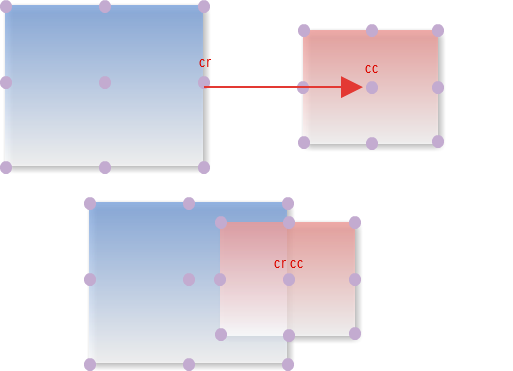
\includegraphics{align.png}
\end{notice}

\end{fulllineitems}


\index{effect (in module Overlay)}

\begin{fulllineitems}
\phantomsection\label{api/component/overlay/overlay:Overlay.effect}\pysigline{\code{Overlay.}\bfcode{effect}}{}~New in version 1.2.
\{Object\} - 可选, 显示或隐藏时的特效支持, 例如:

\begin{Verbatim}[commandchars=\\\{\}]
\PYG{p}{\PYGZob{}}
    \PYG{n+nx}{effect}\PYG{o}{:}\PYG{l+s+s1}{'none'}\PYG{p}{,}    \PYG{c+c1}{// \PYGZob{}String\PYGZcb{} - 可选, 默认为'none', 'none'(无特效), 'fade'(渐隐显示), 'slide'(滑动显示).}
    \PYG{n+nx}{easing}\PYG{o}{:}\PYG{l+s+s1}{''}\PYG{p}{,}        \PYG{c+c1}{// \PYGZob{}String\PYGZcb{} - 可选, 同 KISSY.Anim 的 easing 参数配置.}
    \PYG{n+nx}{duratiion}\PYG{o}{:}\PYG{l+m+mi}{3}       \PYG{c+c1}{// \PYGZob{}Number\PYGZcb{} - 可选, 动画持续时间, 以秒为单位.}
\PYG{p}{\PYGZcb{}}
\end{Verbatim}

\end{fulllineitems}


\index{resize (in module Overlay)}

\begin{fulllineitems}
\phantomsection\label{api/component/overlay/overlay:Overlay.resize}\pysigline{\code{Overlay.}\bfcode{resize}}{}~New in version 1.2.
\{Object\} - 可选, 拖动调整大小的配置, 例如:

\begin{Verbatim}[commandchars=\\\{\}]
\PYG{p}{\PYGZob{}}
    \PYG{n+nx}{minWidth}\PYG{o}{:}\PYG{l+m+mi}{100}\PYG{p}{,} \PYG{c+c1}{//类型整数, 表示拖动调整大小的最小宽度}
    \PYG{n+nx}{maxWidth}\PYG{o}{:}\PYG{l+m+mi}{1000}\PYG{p}{,} \PYG{c+c1}{//类型整数, 表示拖动调整大小的最大宽度}
    \PYG{n+nx}{minHeight}\PYG{o}{:}\PYG{l+m+mi}{100}\PYG{p}{,} \PYG{c+c1}{//类型整数, 表示拖动调整大小的最小高度}
    \PYG{n+nx}{maxHeight}\PYG{o}{:}\PYG{l+m+mi}{1000}\PYG{p}{,} \PYG{c+c1}{//类型整数, 表示拖动调整大小的最大高度}
    \PYG{n+nx}{handlers}\PYG{o}{:}\PYG{p}{[}\PYG{l+s+s2}{"b"}\PYG{p}{,}\PYG{l+s+s2}{"t"}\PYG{p}{,}\PYG{l+s+s2}{"r"}\PYG{p}{,}\PYG{l+s+s2}{"l"}\PYG{p}{,}\PYG{l+s+s2}{"tr"}\PYG{p}{,}\PYG{l+s+s2}{"tl"}\PYG{p}{,}\PYG{l+s+s2}{"br"}\PYG{p}{,}\PYG{l+s+s2}{"bl"}\PYG{p}{]} \PYG{c+c1}{//类型字符串数组, 取自上述 8 个值的集合.}
\PYG{p}{\PYGZcb{}}
\end{Verbatim}

\code{handlers} 配置表示的数组元素可取上述八种值之一, t,b,l,r 分别表示 top,bottom,left,right, 加上组合共八种取值,
可在上, 下, 左, 右以及左上, 左下, 右上, 右下进行拖动.

\end{fulllineitems}



\subparagraph{Properties Detail}
\label{api/component/overlay/overlay:properties-detail}\begin{quote}

当根据配置实例化 overlay 得到当前实例后, 可调用实例上的 get 方法得到实例的特定属性以及 set 方法设置属性的值, 例如

\begin{Verbatim}[commandchars=\\\{\}]
\PYG{k+kd}{var} \PYG{n+nx}{o} \PYG{o}{=} \PYG{k}{new} \PYG{n+nx}{Overlay}\PYG{p}{(}\PYG{p}{\PYGZob{}} \PYG{n+nx}{xy} \PYG{o}{:} \PYG{p}{[}\PYG{l+m+mi}{400}\PYG{p}{,}\PYG{l+m+mi}{200}\PYG{p}{]} \PYG{p}{\PYGZcb{}}\PYG{p}{)}\PYG{p}{;}
\PYG{n+nx}{o}\PYG{p}{.}\PYG{n+nx}{set}\PYG{p}{(}\PYG{l+s+s2}{"xy"}\PYG{p}{,}\PYG{p}{[}\PYG{l+m+mi}{100}\PYG{p}{,}\PYG{l+m+mi}{200}\PYG{p}{]}\PYG{p}{)}\PYG{p}{;}    \PYG{c+c1}{//设置当前实例的绝对坐标}
\PYG{n+nx}{o}\PYG{p}{.}\PYG{n+nx}{get}\PYG{p}{(}\PYG{l+s+s2}{"xy"}\PYG{p}{)}\PYG{p}{;}    \PYG{c+c1}{//获取当前实例的绝对坐标}
\end{Verbatim}
\end{quote}

\index{x (in module Overlay)}

\begin{fulllineitems}
\pysigline{\code{Overlay.}\bfcode{x}}{}
\{Number\} - 悬浮层相对于文档根节点的 x 坐标.

\end{fulllineitems}


\index{y (in module Overlay)}

\begin{fulllineitems}
\pysigline{\code{Overlay.}\bfcode{y}}{}
\{Number\} - 浮层相对于文档根节点的 y 坐标.

\end{fulllineitems}


\index{xy (in module Overlay)}

\begin{fulllineitems}
\pysigline{\code{Overlay.}\bfcode{xy}}{}
\{Array\textless{}Number\textgreater{}\} - 相当于将数组第一个元素设置为 {\hyperref[api/component/overlay/overlay:Overlay.x]{\code{x}}} 的值, 将数组的第二个元素设置为 {\hyperref[api/component/overlay/overlay:Overlay.y]{\code{y}}} 的值.

\end{fulllineitems}


\index{align (in module Overlay)}

\begin{fulllineitems}
\pysigline{\code{Overlay.}\bfcode{align}}{}
\{Object\} - 悬浮层对齐的相关配置.

\end{fulllineitems}


\index{visible (in module Overlay)}

\begin{fulllineitems}
\phantomsection\label{api/component/overlay/overlay:Overlay.visible}\pysigline{\code{Overlay.}\bfcode{visible}}{}
\{Boolean\} - 悬浮层的是否显示.

\end{fulllineitems}


\index{el (in module Overlay)}

\begin{fulllineitems}
\phantomsection\label{api/component/overlay/overlay:Overlay.el}\pysigline{\code{Overlay.}\bfcode{el}}{}
\{KISSY.Node\} - 获取悬浮层的根节点 .

\begin{notice}{note}{Note:}
必须在调用 {\hyperref[api/component/overlay/overlay:Overlay.render]{\code{render()}}} 方法之后才可以获取.
\end{notice}

\end{fulllineitems}


\index{contentEl (in module Overlay)}

\begin{fulllineitems}
\phantomsection\label{api/component/overlay/overlay:Overlay.contentEl}\pysigline{\code{Overlay.}\bfcode{contentEl}}{}
\{KISSY.Node\} - 获取悬浮层真正内容所在的节点.

\begin{notice}{note}{Note:}
必须在调用  {\hyperref[api/component/overlay/overlay:Overlay.render]{\code{render()}}} 方法之后才可以获取.
\end{notice}

悬浮层的 html 结构如下

\begin{Verbatim}[commandchars=\\\{\}]
\PYG{n+nt}{\textless{}div}\PYG{n+nt}{\textgreater{}}\PYG{c}{\textless{}!--}\PYG{c}{ 悬浮层根节点 }\PYG{c}{--\textgreater{}}
    \PYG{n+nt}{\textless{}div}\PYG{n+nt}{\textgreater{}}\PYG{c}{\textless{}!--}\PYG{c}{ 悬浮层内容节点 }\PYG{c}{-}\PYG{c}{--\textgreater{}}
        \PYG{c}{\textless{}!--}\PYG{c}{ 悬浮层真正内容所在 }\PYG{c}{--\textgreater{}}
    \PYG{n+nt}{\textless{}/div\textgreater{}}
\PYG{n+nt}{\textless{}/div\textgreater{}}
\end{Verbatim}

一般调用悬浮层的 {\hyperref[api/component/overlay/overlay:Overlay.render]{\code{render()}}} 方法后, 可通过获取 {\hyperref[api/component/overlay/overlay:Overlay.contentEl]{\code{contentEl}}} 属性获取内容所在节点, 来动态修改悬浮层的内容.

\end{fulllineitems}



\subparagraph{Methods Detail}
\label{api/component/overlay/overlay:methods-detail}
\index{render() (in module Overlay)}

\begin{fulllineitems}
\phantomsection\label{api/component/overlay/overlay:Overlay.render}\pysiglinewithargsret{\code{Overlay.}\bfcode{render}}{}{}~
\begin{DUlineblock}{0em}
\item[] \textbf{render} ()
\item[] 渲染当前实例, 生成对应的 dom 节点并添加到页面文档树中.
\end{DUlineblock}

\end{fulllineitems}


\index{show() (in module Overlay)}

\begin{fulllineitems}
\phantomsection\label{api/component/overlay/overlay:Overlay.show}\pysiglinewithargsret{\code{Overlay.}\bfcode{show}}{}{}~
\begin{DUlineblock}{0em}
\item[] \textbf{show} ()
\item[] 显示悬浮层, 位置根据 {\hyperref[api/component/overlay/overlay:Overlay.align]{\code{align}}} 或者 {\hyperref[api/component/overlay/overlay:Overlay.xy]{\code{xy}}} 确定.
\end{DUlineblock}

\end{fulllineitems}


\index{hide() (in module Overlay)}

\begin{fulllineitems}
\phantomsection\label{api/component/overlay/overlay:Overlay.hide}\pysiglinewithargsret{\code{Overlay.}\bfcode{hide}}{}{}~
\begin{DUlineblock}{0em}
\item[] \textbf{hide} ()
\item[] 隐藏悬浮层.
\end{DUlineblock}

\end{fulllineitems}


\index{align() (in module Overlay)}

\begin{fulllineitems}
\pysiglinewithargsret{\code{Overlay.}\bfcode{align}}{}{}~
\begin{DUlineblock}{0em}
\item[] \textbf{align} (node,points,offset)
\item[] 设置对齐
\end{DUlineblock}
\begin{quote}\begin{description}
\item[{Parameters}] \leavevmode\begin{itemize}
\item {}
\textbf{node} (\emph{string\textbar{}KISSY.Node\textbar{}HTMLDOMNode}) -- 类型对齐的参考元素

\item {}
\textbf{points} (\emph{Array\textless{}string\textgreater{}}) -- 对齐的参考位置

\item {}
\textbf{offset} (\emph{Array\textless{}number\textgreater{}}) -- 相对对齐元素的偏移

\end{itemize}

\end{description}\end{quote}

\begin{notice}{note}{Note:}
调用该方法前请先调用 {\hyperref[api/component/overlay/overlay:Overlay.render]{\code{render()}}}.
\end{notice}

\end{fulllineitems}


\index{center() (in module Overlay)}

\begin{fulllineitems}
\phantomsection\label{api/component/overlay/overlay:Overlay.center}\pysiglinewithargsret{\code{Overlay.}\bfcode{center}}{}{}~
\begin{DUlineblock}{0em}
\item[] \textbf{center} ()
\item[] 将悬浮层放在当前视窗中央.
\end{DUlineblock}

\begin{notice}{note}{Note:}
调用该方法前请先调用 {\hyperref[api/component/overlay/overlay:Overlay.render]{\code{render()}}}.
\end{notice}

\end{fulllineitems}


\index{move() (in module Overlay)}

\begin{fulllineitems}
\phantomsection\label{api/component/overlay/overlay:Overlay.move}\pysiglinewithargsret{\code{Overlay.}\bfcode{move}}{}{}~
\begin{DUlineblock}{0em}
\item[] \textbf{move} (x,y)
\item[] 设置悬浮层相对于文档左上角的坐标偏移
\end{DUlineblock}
\begin{quote}\begin{description}
\item[{Parameters}] \leavevmode\begin{itemize}
\item {}
\textbf{x} (\emph{number}) -- 横坐标偏移量

\item {}
\textbf{y} (\emph{number}) -- 纵坐标偏移量

\end{itemize}

\end{description}\end{quote}

\end{fulllineitems}



\subparagraph{Events Detail}
\label{api/component/overlay/overlay:events-detail}
\index{hide() (in module Overlay)}

\begin{fulllineitems}
\pysiglinewithargsret{\code{Overlay.}\bfcode{hide}}{}{}~
\begin{DUlineblock}{0em}
\item[] \textbf{hide} ()
\item[] 当悬浮层隐藏时触发
\end{DUlineblock}

\end{fulllineitems}


\index{show() (in module Overlay)}

\begin{fulllineitems}
\pysiglinewithargsret{\code{Overlay.}\bfcode{show}}{}{}~
\begin{DUlineblock}{0em}
\item[] \textbf{show} ()
\item[] 当悬浮层显示时触发
\end{DUlineblock}

\end{fulllineitems}


\index{beforeVisibleChange() (in module Overlay)}

\begin{fulllineitems}
\phantomsection\label{api/component/overlay/overlay:Overlay.beforeVisibleChange}\pysiglinewithargsret{\code{Overlay.}\bfcode{beforeVisibleChange}}{}{}~
\begin{DUlineblock}{0em}
\item[] \textbf{beforeVisibleChange} (ev)
\item[] 当悬浮层隐藏或显示前触发
\end{DUlineblock}
\begin{quote}\begin{description}
\item[{Parameters}] \leavevmode\begin{itemize}
\item {}
\textbf{ev.newVal} (\emph{Boolean}) -- 将要隐藏时为 false, 将要显示时为 true

\item {}
\textbf{ev.prevVal} (\emph{Boolean}) -- 当前悬浮层显示与否

\end{itemize}

\item[{Returns}] \leavevmode
\{Boolean\} - 返回 false 时, 则会阻止将要进行的显示或隐藏动作.

\end{description}\end{quote}

\end{fulllineitems}

\phantomsection\label{api/component/overlay/dialog:module-Overlay}
\index{Overlay (module)}

\paragraph{Dialog}
\label{api/component/overlay/dialog::doc}\label{api/component/overlay/dialog:dialog}
\begin{DUlineblock}{0em}
\item[] 对话框.
\item[] 扩展于 {\hyperref[api/component/overlay/popup:module-Overlay]{\code{Overlay}}}
\item[] 作者: \href{mailto:yiminghe@gmail.com}{承玉}
\item[] \href{https://github.com/kissyteam/kissy/tree/master/src/overlay/}{源码}  \textbar{} Demo
\end{DUlineblock}


\subparagraph{Class}
\label{api/component/overlay/dialog:class}\begin{itemize}
\item {}
{\hyperref[api/component/overlay/dialog:Overlay.Dialog]{\code{Dialog}}}

\end{itemize}


\subparagraph{Config Attributes}
\label{api/component/overlay/dialog:config-attributes}\begin{quote}

除了 {\hyperref[api/component/overlay/overlay:Overlay.content]{\code{content}}} 配置项外与 {\hyperref[api/component/overlay/popup:module-Overlay]{\code{Overlay}}} 的配置项完全相同, 其他新增配置项如下:
\begin{itemize}
\item {}
{\hyperref[api/component/overlay/dialog:Overlay.headerContent]{\code{headerContent}}}

\item {}
{\hyperref[api/component/overlay/dialog:Overlay.bodyContent]{\code{bodyContent}}}

\item {}
{\hyperref[api/component/overlay/dialog:Overlay.footerContent]{\code{footerContent}}}

\item {}
{\hyperref[api/component/overlay/dialog:Overlay.closable]{\code{closable}}}

\item {}
{\hyperref[api/component/overlay/dialog:Overlay.draggable]{\code{draggable}}}

\item {}
{\hyperref[api/component/overlay/dialog:Overlay.aria]{\code{aria}}}

\item {}
{\hyperref[api/component/overlay/dialog:Overlay.constrain]{\code{constrain}}}

\end{itemize}
\end{quote}


\subparagraph{Properties}
\label{api/component/overlay/dialog:properties}\begin{quote}

除了 {\hyperref[api/component/overlay/popup:module-Overlay]{\code{Overlay}}} 的所有属性之外还有:
\begin{itemize}
\item {}
{\hyperref[api/component/overlay/dialog:Overlay.header]{\code{header}}}

\item {}
{\hyperref[api/component/overlay/dialog:Overlay.body]{\code{body}}}

\item {}
{\hyperref[api/component/overlay/dialog:Overlay.footer]{\code{footer}}}

\item {}
{\hyperref[api/component/overlay/dialog:Overlay.closable]{\code{closable}}}

\item {}
{\hyperref[api/component/overlay/dialog:Overlay.draggable]{\code{draggable}}}

\item {}
{\hyperref[api/component/overlay/dialog:Overlay.constrain]{\code{constrain}}}

\end{itemize}
\end{quote}


\subparagraph{Methods}
\label{api/component/overlay/dialog:methods}\begin{itemize}
\item {}
同 {\hyperref[api/component/overlay/popup:module-Overlay]{\code{Overlay}}} .

\end{itemize}


\subparagraph{Events}
\label{api/component/overlay/dialog:events}\begin{itemize}
\item {}
同 {\hyperref[api/component/overlay/popup:module-Overlay]{\code{Overlay}}} , 包括 {\hyperref[api/component/overlay/overlay:Overlay.show]{\code{show()}}} , {\hyperref[api/component/overlay/overlay:Overlay.hide]{\code{hide()}}} , {\hyperref[api/component/overlay/overlay:Overlay.beforeVisibleChange]{\code{beforeVisibleChange()}}} .

\end{itemize}


\subparagraph{Class Detail}
\label{api/component/overlay/dialog:class-detail}
\index{Dialog (class in Overlay)}

\begin{fulllineitems}
\phantomsection\label{api/component/overlay/dialog:Overlay.Dialog}\pysigline{\strong{class }\code{Overlay.}\bfcode{Dialog}}{}~
\begin{DUlineblock}{0em}
\item[] \textbf{Dialog} (config)
\end{DUlineblock}
\begin{quote}\begin{description}
\item[{Parameters}] \leavevmode
\textbf{config} (\emph{Object}) -- 配置项, 详细见下方 \textbf{Config Attributes Detail} .

\end{description}\end{quote}

对话框的 DOM 结构为:

\begin{Verbatim}[commandchars=\\\{\}]
\PYG{n+nt}{\textless{}div}\PYG{n+nt}{\textgreater{}} \PYG{c}{\textless{}!--}\PYG{c}{ 对话框根节点 }\PYG{c}{--\textgreater{}}
    \PYG{n+nt}{\textless{}div}\PYG{n+nt}{\textgreater{}} \PYG{c}{\textless{}!--}\PYG{c}{ 对话框内容节点 }\PYG{c}{--\textgreater{}}
        \PYG{n+nt}{\textless{}div}\PYG{n+nt}{\textgreater{}} \PYG{c}{\textless{}!--}\PYG{c}{ 对话框标题节点 }\PYG{c}{--\textgreater{}}
        \PYG{n+nt}{\textless{}/div\textgreater{}}

        \PYG{n+nt}{\textless{}div}\PYG{n+nt}{\textgreater{}} \PYG{c}{\textless{}!--}\PYG{c}{ 对话框体节点 }\PYG{c}{--\textgreater{}}
        \PYG{n+nt}{\textless{}/div\textgreater{}}

        \PYG{n+nt}{\textless{}div}\PYG{n+nt}{\textgreater{}} \PYG{c}{\textless{}!--}\PYG{c}{ 对话框底部节点 }\PYG{c}{--\textgreater{}}
        \PYG{n+nt}{\textless{}/div\textgreater{}}
    \PYG{n+nt}{\textless{}/div\textgreater{}}
\PYG{n+nt}{\textless{}/div\textgreater{}}
\end{Verbatim}

\end{fulllineitems}



\subparagraph{Config Attributes Detail}
\label{api/component/overlay/dialog:config-attributes-detail}\begin{quote}

除了 {\hyperref[api/component/overlay/overlay:Overlay.content]{\code{content}}} 配置项外与 {\hyperref[api/component/overlay/popup:module-Overlay]{\code{Overlay}}} 的配置项完全相同, 但是新增了一些配置项如下所示:
\end{quote}

\index{headerContent (in module Overlay)}

\begin{fulllineitems}
\phantomsection\label{api/component/overlay/dialog:Overlay.headerContent}\pysigline{\code{Overlay.}\bfcode{headerContent}}{}
\{String\} - 对话框的标题 html.

\end{fulllineitems}


\index{bodyContent (in module Overlay)}

\begin{fulllineitems}
\phantomsection\label{api/component/overlay/dialog:Overlay.bodyContent}\pysigline{\code{Overlay.}\bfcode{bodyContent}}{}
\{String\} - 对话框的体 html.

\end{fulllineitems}


\index{footerContent (in module Overlay)}

\begin{fulllineitems}
\phantomsection\label{api/component/overlay/dialog:Overlay.footerContent}\pysigline{\code{Overlay.}\bfcode{footerContent}}{}
\{String\} - 对话框的底部 html.

\end{fulllineitems}


\index{closable (in module Overlay)}

\begin{fulllineitems}
\phantomsection\label{api/component/overlay/dialog:Overlay.closable}\pysigline{\code{Overlay.}\bfcode{closable}}{}
\{Boolean\} - 对话框右上角是否包括关闭按钮

\end{fulllineitems}


\index{draggable (in module Overlay)}

\begin{fulllineitems}
\phantomsection\label{api/component/overlay/dialog:Overlay.draggable}\pysigline{\code{Overlay.}\bfcode{draggable}}{}
\{Boolean\} - 是否允许拖动头部移动, 注意启用时需同时 \code{use("dd")} , 例如:

\begin{Verbatim}[commandchars=\\\{\}]
\PYG{n+nx}{KISSY}\PYG{p}{.}\PYG{n+nx}{use}\PYG{p}{(}\PYG{l+s+s2}{"dd,overlay"}\PYG{p}{,}\PYG{k+kd}{function}\PYG{p}{(}\PYG{n+nx}{S}\PYG{p}{,}\PYG{n+nx}{DD}\PYG{p}{,}\PYG{n+nx}{Overlay}\PYG{p}{)}\PYG{p}{\PYGZob{}}
    \PYG{k}{new} \PYG{n+nx}{Overlay}\PYG{p}{.}\PYG{n+nx}{Dialog}\PYG{p}{(}\PYG{p}{\PYGZob{}}
        \PYG{n+nx}{draggable} \PYG{o}{:} \PYG{k+kc}{true}
    \PYG{p}{\PYGZcb{}}\PYG{p}{)}\PYG{p}{;}
\PYG{p}{\PYGZcb{}}\PYG{p}{)}\PYG{p}{;}
\end{Verbatim}

\end{fulllineitems}


\index{aria (in module Overlay)}

\begin{fulllineitems}
\phantomsection\label{api/component/overlay/dialog:Overlay.aria}\pysigline{\code{Overlay.}\bfcode{aria}}{}
\{Boolean\} - 默认为 false, 是否开启 aria 支持. 开启后, 窗口显示出来时自动获得焦点并且 tab 键只能在窗口内部转移焦点.
New in version 1.2.
\end{fulllineitems}


\index{constrain (in module Overlay)}

\begin{fulllineitems}
\phantomsection\label{api/component/overlay/dialog:Overlay.constrain}\pysigline{\code{Overlay.}\bfcode{constrain}}{}~\begin{description}
\item[{\{Boolean \textbar{} String\} - 和 {\hyperref[api/component/dd/draggable:Draggable.Draggable]{\code{Draggable}}} 配合, 限制拖动的范围.}] \leavevmode\begin{itemize}
\item {}
取值选择器字符串时, 则在限制拖动范围为根据该选择器字符串取到的第一个节点所在区域.

\item {}
取值 true 时, 只能在当前视窗范围内拖动.

\item {}
取值 false 时, 可任意移动, 例如:

\end{itemize}

\end{description}

\begin{Verbatim}[commandchars=\\\{\}]
\PYG{n+nx}{KISSY}\PYG{p}{.}\PYG{n+nx}{use}\PYG{p}{(}\PYG{l+s+s2}{"dd,overlay"}\PYG{p}{,}\PYG{k+kd}{function}\PYG{p}{(}\PYG{n+nx}{S}\PYG{p}{,}\PYG{n+nx}{DD}\PYG{p}{,}\PYG{n+nx}{Overlay}\PYG{p}{)}\PYG{p}{\PYGZob{}}
    \PYG{k}{new} \PYG{n+nx}{Overlay}\PYG{p}{.}\PYG{n+nx}{Dialog}\PYG{p}{(}\PYG{p}{\PYGZob{}}
        \PYG{n+nx}{draggable} \PYG{o}{:} \PYG{k+kc}{true}\PYG{p}{,}
        \PYG{n+nx}{contrain}\PYG{o}{:}\PYG{k+kc}{true} \PYG{c+c1}{// 限制拖动区域为当前视窗范围}
    \PYG{p}{\PYGZcb{}}\PYG{p}{)}\PYG{p}{;}
\PYG{p}{\PYGZcb{}}\PYG{p}{)}\PYG{p}{;}

\PYG{n+nx}{KISSY}\PYG{p}{.}\PYG{n+nx}{use}\PYG{p}{(}\PYG{l+s+s2}{"dd,overlay"}\PYG{p}{,}\PYG{k+kd}{function}\PYG{p}{(}\PYG{n+nx}{S}\PYG{p}{,}\PYG{n+nx}{DD}\PYG{p}{,}\PYG{n+nx}{Overlay}\PYG{p}{)}\PYG{p}{\PYGZob{}}
    \PYG{k}{new} \PYG{n+nx}{Overlay}\PYG{p}{.}\PYG{n+nx}{Dialog}\PYG{p}{(}\PYG{p}{\PYGZob{}}
        \PYG{n+nx}{draggable} \PYG{o}{:} \PYG{k+kc}{true}\PYG{p}{,}
        \PYG{n+nx}{contrain}\PYG{o}{:}\PYG{l+s+s2}{"\#container"} \PYG{c+c1}{// 限制拖动区域为 container 节点所占据区域}
    \PYG{p}{\PYGZcb{}}\PYG{p}{)}\PYG{p}{;}
\PYG{p}{\PYGZcb{}}\PYG{p}{)}\PYG{p}{;}
\end{Verbatim}

\end{fulllineitems}



\subparagraph{Properties Detail}
\label{api/component/overlay/dialog:properties-detail}\begin{quote}

除了 {\hyperref[api/component/overlay/popup:module-Overlay]{\code{Overlay}}} 的所有属性之外还有:
\end{quote}

\index{header (in module Overlay)}

\begin{fulllineitems}
\phantomsection\label{api/component/overlay/dialog:Overlay.header}\pysigline{\code{Overlay.}\bfcode{header}}{}
\{KISSY.Node\} - 只读, 对话框的头部节点.

\end{fulllineitems}


\index{body (in module Overlay)}

\begin{fulllineitems}
\phantomsection\label{api/component/overlay/dialog:Overlay.body}\pysigline{\code{Overlay.}\bfcode{body}}{}
\{KISSY.Node\} - 只读, 对话框的体部节点.

\end{fulllineitems}


\index{footer (in module Overlay)}

\begin{fulllineitems}
\phantomsection\label{api/component/overlay/dialog:Overlay.footer}\pysigline{\code{Overlay.}\bfcode{footer}}{}
\{KISSY.Node\} - 只读, 对话框的底部节点.

\begin{notice}{note}{Note:}
以上三个属性在获取前必须调用过 \code{render()} 方法.
\end{notice}

\end{fulllineitems}


\index{closable (in module Overlay)}

\begin{fulllineitems}
\pysigline{\code{Overlay.}\bfcode{closable}}{}
\{Boolean\} - 右上角拖放区域有无.

\end{fulllineitems}


\index{draggable (in module Overlay)}

\begin{fulllineitems}
\pysigline{\code{Overlay.}\bfcode{draggable}}{}
\{Boolean\} - 头部是否可以拖放.

\end{fulllineitems}


\index{constrain (in module Overlay)}

\begin{fulllineitems}
\pysigline{\code{Overlay.}\bfcode{constrain}}{}
\{Boolean \textbar{} String\} - 拖放区域范围.

\end{fulllineitems}



\subparagraph{Methods Detail}
\label{api/component/overlay/dialog:methods-detail}\begin{quote}

同 {\hyperref[api/component/overlay/popup:module-Overlay]{\code{Overlay}}} .
\end{quote}


\subparagraph{Events Detail}
\label{api/component/overlay/dialog:events-detail}\begin{quote}

同 {\hyperref[api/component/overlay/popup:module-Overlay]{\code{Overlay}}} , 包括 {\hyperref[api/component/overlay/overlay:Overlay.show]{\code{show()}}} , {\hyperref[api/component/overlay/overlay:Overlay.hide]{\code{hide()}}} , {\hyperref[api/component/overlay/overlay:Overlay.beforeVisibleChange]{\code{beforeVisibleChange()}}} .
\end{quote}
\phantomsection\label{api/component/overlay/popup:module-Overlay}
\index{Overlay (module)}

\paragraph{Popup}
\label{api/component/overlay/popup:popup}\label{api/component/overlay/popup::doc}
\begin{DUlineblock}{0em}
\item[] 弹出层
\item[] 作者: \href{mailto:qiaohua@taobao.com}{乔花}
\item[] \href{https://github.com/kissyteam/kissy/tree/master/src/overlay/}{源码}  \textbar{} Demo
\end{DUlineblock}


\subparagraph{Class}
\label{api/component/overlay/popup:class}\begin{itemize}
\item {}
{\hyperref[api/component/overlay/popup:Overlay.Popup]{\code{Popup}}}

\end{itemize}


\subparagraph{Config Attributes}
\label{api/component/overlay/popup:config-attributes}\begin{quote}

与 {\hyperref[api/component/overlay/popup:module-Overlay]{\code{Overlay}}} 的配置项完全相同, 其他新增配置项如下:
\begin{itemize}
\item {}
{\hyperref[api/component/overlay/popup:Overlay.trigger]{\code{trigger}}}

\item {}
{\hyperref[api/component/overlay/popup:Overlay.triggerType]{\code{triggerType}}}

\end{itemize}
\end{quote}


\subparagraph{Properties}
\label{api/component/overlay/popup:properties}\begin{itemize}
\item {}
同 {\hyperref[api/component/overlay/popup:module-Overlay]{\code{Overlay}}} .

\end{itemize}


\subparagraph{Methods}
\label{api/component/overlay/popup:methods}\begin{itemize}
\item {}
同 {\hyperref[api/component/overlay/popup:module-Overlay]{\code{Overlay}}} .

\end{itemize}


\subparagraph{Events}
\label{api/component/overlay/popup:events}\begin{itemize}
\item {}
同 {\hyperref[api/component/overlay/popup:module-Overlay]{\code{Overlay}}} , 包括 {\hyperref[api/component/overlay/overlay:Overlay.show]{\code{show()}}} , {\hyperref[api/component/overlay/overlay:Overlay.hide]{\code{hide()}}} , {\hyperref[api/component/overlay/overlay:Overlay.beforeVisibleChange]{\code{beforeVisibleChange()}}} .

\end{itemize}


\subparagraph{Class Detail}
\label{api/component/overlay/popup:class-detail}
\index{Popup (class in Overlay)}

\begin{fulllineitems}
\phantomsection\label{api/component/overlay/popup:Overlay.Popup}\pysigline{\strong{class }\code{Overlay.}\bfcode{Popup}}{}~
\begin{DUlineblock}{0em}
\item[] \textbf{Popup} ({[}container,{]} config)
\end{DUlineblock}
\begin{quote}\begin{description}
\item[{Parameters}] \leavevmode\begin{itemize}
\item {}
\textbf{container} (\emph{String\textbar{}HTMLElement\textbar{}KISSY.Node}) -- 可为'\#id'、'.class'、DOM对象、KISSY.Node对象, 为空时表示新建

\item {}
\textbf{config} (\emph{Object}) -- 配置项, 详细见下方 \textbf{Config Attributes Detail} .

\end{itemize}

\end{description}\end{quote}

\end{fulllineitems}



\subparagraph{Config Attributes Detail}
\label{api/component/overlay/popup:config-attributes-detail}\begin{quote}

与 {\hyperref[api/component/overlay/popup:module-Overlay]{\code{Overlay}}} 的配置项完全相同, 其他新增配置项如下:
\end{quote}

\index{trigger (in module Overlay)}

\begin{fulllineitems}
\phantomsection\label{api/component/overlay/popup:Overlay.trigger}\pysigline{\code{Overlay.}\bfcode{trigger}}{}
\{String \textbar{} HTMLElement \textbar{} KISSY.Node\} - 触点

\end{fulllineitems}


\index{triggerType (in module Overlay)}

\begin{fulllineitems}
\phantomsection\label{api/component/overlay/popup:Overlay.triggerType}\pysigline{\code{Overlay.}\bfcode{triggerType}}{}
\{String\} - 可选, 默认为'click', 触发类型, 可选'click'、'mouse'.

\end{fulllineitems}



\subparagraph{Properties Detail}
\label{api/component/overlay/popup:properties-detail}\begin{quote}

同 {\hyperref[api/component/overlay/popup:module-Overlay]{\code{Overlay}}} .
\end{quote}


\subparagraph{Methods Detail}
\label{api/component/overlay/popup:methods-detail}\begin{quote}

同 {\hyperref[api/component/overlay/popup:module-Overlay]{\code{Overlay}}} .
\end{quote}


\subparagraph{Events Detail}
\label{api/component/overlay/popup:events-detail}\begin{quote}

同 {\hyperref[api/component/overlay/popup:module-Overlay]{\code{Overlay}}} , 包括 {\hyperref[api/component/overlay/overlay:Overlay.show]{\code{show()}}} , {\hyperref[api/component/overlay/overlay:Overlay.hide]{\code{hide()}}} , {\hyperref[api/component/overlay/overlay:Overlay.beforeVisibleChange]{\code{beforeVisibleChange()}}} .
\end{quote}


\chapter{All Demos}
\label{demo/index:demo}\label{demo/index::doc}\label{demo/index:all-demos}

\section{Seed}
\label{demo/seed/index:seed-demo}\label{demo/seed/index:seed}\label{demo/seed/index::doc}
\begin{DUlineblock}{0em}
\item[] 作者: \href{mailto:yiminghe@gmail.com}{承玉}
\item[] 源码: \href{https://github.com/kissyteam/kissy/tree/master/src/seed}{查看}
\end{DUlineblock}


\subsection{Loader Demos}
\label{demo/seed/loader/index:loader-demos}\label{demo/seed/loader/index::doc}

\subsubsection{Module}
\label{demo/seed/loader/index:module}\begin{quote}

{\hyperref[api/seed/loader/index:module-Loader]{\code{Loader}}}
\end{quote}


\subsubsection{Demo - 1.1.x 的 Loader 使用示例}
\label{demo/seed/loader/index:demo-1-1-x-loader}\label{demo/seed/loader/index:seed-loader-demo1}\begin{quote}

\textbf{注册模块}

\begin{Verbatim}[commandchars=\\\{\}]
\PYG{n+nx}{KISSY}\PYG{p}{.}\PYG{n+nx}{add}\PYG{p}{(}\PYG{p}{\PYGZob{}}
   \PYG{l+s+s2}{"1.1x-dep"}\PYG{o}{:}\PYG{p}{\PYGZob{}}
        \PYG{n+nx}{fullpath}\PYG{o}{:}\PYG{l+s+s2}{"http://lite-ext.googlecode.com/svn/trunk/lite-ext/playground/module\PYGZus{}package/1.1x/dep.js"}
   \PYG{p}{\PYGZcb{}}\PYG{p}{,}
   \PYG{l+s+s2}{"1.1x-mod"}\PYG{o}{:}\PYG{p}{\PYGZob{}}
        \PYG{n+nx}{fullpath}\PYG{o}{:}\PYG{l+s+s2}{"http://lite-ext.googlecode.com/svn/trunk/lite-ext/playground/module\PYGZus{}package/1.1x/mod.js"}\PYG{p}{,}
        \PYG{n+nx}{cssfullpath}\PYG{o}{:}\PYG{l+s+s2}{"http://lite-ext.googlecode.com/svn/trunk/lite-ext/playground/module\PYGZus{}package/1.1x/mod.css"}\PYG{p}{,}
        \PYG{n+nx}{requires}\PYG{o}{:}\PYG{p}{[}\PYG{l+s+s2}{"1.1x-dep"}\PYG{p}{]}
   \PYG{p}{\PYGZcb{}}
\PYG{p}{\PYGZcb{}}\PYG{p}{)}\PYG{p}{;}
\end{Verbatim}

\textbf{定义模块}

\href{http://lite-ext.googlecode.com/svn/trunk/lite-ext/playground/module\_package/1.1x/dep.js}{被依赖模块 1.1x dep}

\begin{Verbatim}[commandchars=\\\{\}]
\PYG{n+nx}{KISSY}\PYG{p}{.}\PYG{n+nx}{add}\PYG{p}{(}\PYG{l+s+s2}{"1.1x-dep"}\PYG{p}{,}\PYG{k+kd}{function}\PYG{p}{(}\PYG{p}{)}\PYG{p}{\PYGZob{}}
    \PYG{n+nx}{alert}\PYG{p}{(}\PYG{l+s+s2}{"1.1x-dep loaded"}\PYG{p}{)}\PYG{p}{;}
\PYG{p}{\PYGZcb{}}\PYG{p}{)}\PYG{p}{;}
\end{Verbatim}

\href{http://lite-ext.googlecode.com/svn/trunk/lite-ext/playground/module\_package/1.1x/mod.js}{主模块 1.1x mod}

\begin{Verbatim}[commandchars=\\\{\}]
\PYG{n+nx}{KISSY}\PYG{p}{.}\PYG{n+nx}{add}\PYG{p}{(}\PYG{l+s+s2}{"1.1x-mod"}\PYG{p}{,}\PYG{k+kd}{function}\PYG{p}{(}\PYG{p}{)}\PYG{p}{\PYGZob{}}
    \PYG{n+nx}{alert}\PYG{p}{(}\PYG{l+s+s2}{"1.1x-mod loaded"}\PYG{p}{)}\PYG{p}{;}
\PYG{p}{\PYGZcb{}}\PYG{p}{)}\PYG{p}{;}
\end{Verbatim}

\textbf{使用模块}

\begin{Verbatim}[commandchars=\\\{\}]
\PYG{n+nx}{KISSY}\PYG{p}{.}\PYG{n+nx}{use}\PYG{p}{(}\PYG{l+s+s2}{"1.1x-mod"}\PYG{p}{)}\PYG{p}{;}
\end{Verbatim}
\end{quote}


\subsubsection{Demo - 1.2 的 Loader 使用示例}
\label{demo/seed/loader/index:demo-1-2-loader}\label{demo/seed/loader/index:seed-loader-demo2}\begin{quote}

\textbf{包配置}

\begin{Verbatim}[commandchars=\\\{\}]
\PYG{n+nx}{KISSY}\PYG{p}{.}\PYG{n+nx}{config}\PYG{p}{(}\PYG{p}{\PYGZob{}}
    \PYG{n+nx}{packages}\PYG{o}{:}\PYG{p}{[}
        \PYG{p}{\PYGZob{}}
            \PYG{n+nx}{name}\PYG{o}{:}\PYG{l+s+s2}{"1.2"}\PYG{p}{,} \PYG{c+c1}{//包名}
            \PYG{n+nx}{tag}\PYG{o}{:}\PYG{l+s+s2}{"20110323"}\PYG{p}{,}\PYG{c+c1}{//时间戳, 添加在动态脚本路径后面, 用于更新包内模块代码}
            \PYG{n+nx}{path}\PYG{o}{:}\PYG{l+s+s2}{"http://lite-ext.googlecode.com/svn/trunk/lite-ext/playground/module\PYGZus{}package/"}\PYG{p}{,} \PYG{c+c1}{//包对应路径, 相对路径指相对于当前页面路径}
            \PYG{n+nx}{charset}\PYG{o}{:}\PYG{l+s+s2}{"gbk"} \PYG{c+c1}{//包里模块文件编码格式}
        \PYG{p}{\PYGZcb{}}
    \PYG{p}{]}
\PYG{p}{\PYGZcb{}}\PYG{p}{)}\PYG{p}{;}
\end{Verbatim}

\textbf{定义模块}

\href{http://lite-ext.googlecode.com/svn/trunk/lite-ext/playground/module\_package/1.2/dep.js}{被依赖模块 1.2 dep}

\begin{Verbatim}[commandchars=\\\{\}]
\PYG{n+nx}{KISSY}\PYG{p}{.}\PYG{n+nx}{add}\PYG{p}{(}\PYG{k+kd}{function}\PYG{p}{(}\PYG{p}{)}\PYG{p}{\PYGZob{}}
    \PYG{n+nx}{alert}\PYG{p}{(}\PYG{l+s+s2}{"1.2/dep loaded"}\PYG{p}{)}\PYG{p}{;}
\PYG{p}{\PYGZcb{}}\PYG{p}{)}\PYG{p}{;}
\end{Verbatim}

\href{http://lite-ext.googlecode.com/svn/trunk/lite-ext/playground/module\_package/1.2/mod.js}{主模块 1.2 mod}

\begin{Verbatim}[commandchars=\\\{\}]
\PYG{n+nx}{KISSY}\PYG{p}{.}\PYG{n+nx}{add}\PYG{p}{(}\PYG{k+kd}{function}\PYG{p}{(}\PYG{p}{)}\PYG{p}{\PYGZob{}}
    \PYG{n+nx}{alert}\PYG{p}{(}\PYG{l+s+s2}{"1.2/mod loaded"}\PYG{p}{)}\PYG{p}{;}
\PYG{p}{\PYGZcb{}}\PYG{p}{,}\PYG{p}{\PYGZob{}}
    \PYG{n+nx}{requires}\PYG{o}{:}\PYG{p}{[}\PYG{l+s+s2}{"./dep"}\PYG{p}{,}\PYG{l+s+s2}{"./mod.css"}\PYG{p}{]} \PYG{c+c1}{//相对于当前模块js 定位}
\PYG{p}{\PYGZcb{}}\PYG{p}{)}\PYG{p}{;}
\end{Verbatim}

\textbf{使用模块}

\begin{Verbatim}[commandchars=\\\{\}]
\PYG{n+nx}{KISSY}\PYG{p}{.}\PYG{n+nx}{use}\PYG{p}{(}\PYG{l+s+s2}{"1.2/mod"}\PYG{p}{)}\PYG{p}{;}
\end{Verbatim}
\end{quote}


\subsection{Demos}
\label{demo/seed/index:demos}\begin{itemize}
\item {}
{\hyperref[demo/seed/loader/index:seed-loader-demo1]{\emph{Loader - 1.1.x 的 Loader 使用示例}}}

\item {}
{\hyperref[demo/seed/loader/index:seed-loader-demo2]{\emph{Loader - 1.2 的 Loader 使用示例}}}

\end{itemize}


\section{Core}
\label{demo/core/index:core}\label{demo/core/index:core-demo}\label{demo/core/index::doc}
\begin{DUlineblock}{0em}
\item[] KISSY 核心
\item[] 作者: \href{mailto:lifesinger@gmail.com}{玉伯} , \href{mailto:yiminghe@gmail.com}{承玉}
\end{DUlineblock}


\subsection{Anim Demos}
\label{demo/core/anim/index::doc}\label{demo/core/anim/index:anim-demos}

\subsubsection{Class}
\label{demo/core/anim/index:class}\begin{itemize}
\item {}
{\hyperref[api/core/anim/index:module-Anim]{\code{Anim}}}

\end{itemize}


\subsubsection{Demo - 基本动画示例}
\label{demo/core/anim/index:demo}\label{demo/core/anim/index:core-anim-demo1}\begin{quote}

源码:

\begin{Verbatim}[commandchars=\\\{\}]
\PYG{n+nx}{KISSY}\PYG{p}{.}\PYG{n+nx}{use}\PYG{p}{(}\PYG{l+s+s2}{"anim,node"}\PYG{p}{,}\PYG{k+kd}{function}\PYG{p}{(}\PYG{n+nx}{S}\PYG{p}{,}\PYG{n+nx}{Anim}\PYG{p}{,}\PYG{n+nx}{Node}\PYG{p}{)}\PYG{p}{\PYGZob{}}
    \PYG{c+c1}{//KISSY 1.2 以前可通过 var Node=S.Node ; var Anim=S.Anim}
     \PYG{k+kd}{var} \PYG{n+nx}{anim} \PYG{o}{=} \PYG{n+nx}{Anim}\PYG{p}{(}
                \PYG{l+s+s1}{'\#test1'}\PYG{p}{,}
                \PYG{p}{\PYGZob{}}
                    \PYG{l+s+s1}{'background-color'}\PYG{o}{:}\PYG{l+s+s1}{'\#fcc'}\PYG{p}{,}
                    \PYG{c+c1}{//'border': '5px dashed \#999',}
                    \PYG{l+s+s1}{'border-wdith'}\PYG{o}{:}\PYG{l+s+s1}{'5px'}\PYG{p}{,}
                    \PYG{l+s+s1}{'border-color'}\PYG{o}{:}\PYG{l+s+s2}{"\#999999"}\PYG{p}{,}
                    \PYG{l+s+s1}{'border-style'}\PYG{o}{:}\PYG{l+s+s2}{"dashed"}\PYG{p}{,}
                    \PYG{l+s+s1}{'width'}\PYG{o}{:} \PYG{l+s+s1}{'100px'}\PYG{p}{,}
                    \PYG{l+s+s1}{'height'}\PYG{o}{:} \PYG{l+s+s1}{'50px'}\PYG{p}{,}
                    \PYG{l+s+s1}{'left'}\PYG{o}{:} \PYG{l+s+s1}{'900px'}\PYG{p}{,}
                    \PYG{l+s+s1}{'top'}\PYG{o}{:} \PYG{l+s+s1}{'285px'}\PYG{p}{,}
                    \PYG{l+s+s1}{'opacity'}\PYG{o}{:} \PYG{l+s+s1}{'.5'}\PYG{p}{,}
                    \PYG{l+s+s1}{'font-size'}\PYG{o}{:} \PYG{l+s+s1}{'48px'}\PYG{p}{,}
                    \PYG{l+s+s1}{'padding'}\PYG{o}{:} \PYG{l+s+s1}{'30px 0'}\PYG{p}{,}
                    \PYG{l+s+s1}{'color'}\PYG{o}{:} \PYG{l+s+s1}{'\#FF3333'}
                \PYG{p}{\PYGZcb{}}\PYG{p}{,}\PYG{l+m+mi}{5}\PYG{p}{,}
                \PYG{l+s+s1}{'bounceOut'}\PYG{p}{,}\PYG{k+kd}{function}\PYG{p}{(}\PYG{p}{)}\PYG{p}{\PYGZob{}}
                    \PYG{n+nx}{alert}\PYG{p}{(}\PYG{l+s+s1}{'demo1 结束'}\PYG{p}{)}\PYG{p}{;}
                \PYG{p}{\PYGZcb{}}\PYG{p}{)}\PYG{p}{;}
     \PYG{n+nx}{S}\PYG{p}{.}\PYG{n+nx}{one}\PYG{p}{(}\PYG{l+s+s2}{"\#test1-btn"}\PYG{p}{)}\PYG{p}{.}\PYG{n+nx}{on}\PYG{p}{(}\PYG{l+s+s2}{"click"}\PYG{p}{,}\PYG{k+kd}{function}\PYG{p}{(}\PYG{p}{)}\PYG{p}{\PYGZob{}}
        \PYG{n+nx}{anim}\PYG{p}{.}\PYG{n+nx}{run}\PYG{p}{(}\PYG{p}{)}\PYG{p}{;}
     \PYG{p}{\PYGZcb{}}\PYG{p}{)}\PYG{p}{;}
\PYG{p}{\PYGZcb{}}\PYG{p}{)}\PYG{p}{;}
\end{Verbatim}
\end{quote}


\subsubsection{Demo - 滚动属性动画实例}
\label{demo/core/anim/index:core-anim-demo2}\label{demo/core/anim/index:id1}New in version 1.2.

\subsubsection{Demo - 节点实例动画操作}
\label{demo/core/anim/index:id2}\label{demo/core/anim/index:core-anim-demo3}\begin{quote}

源码:

\begin{Verbatim}[commandchars=\\\{\}]
\PYG{n+nx}{KISSY}\PYG{p}{.}\PYG{n+nx}{use}\PYG{p}{(}\PYG{l+s+s2}{"anim,node"}\PYG{p}{,}\PYG{k+kd}{function}\PYG{p}{(}\PYG{n+nx}{S}\PYG{p}{,}\PYG{n+nx}{Anim}\PYG{p}{,}\PYG{n+nx}{Node}\PYG{p}{)}\PYG{p}{\PYGZob{}}
    \PYG{c+c1}{//KISSY 1.2 以前可通过 var Node=S.Node ; var Anim=S.Anim}
    \PYG{k+kd}{var} \PYG{n+nx}{demo\PYGZus{}show}\PYG{o}{=}\PYG{n+nx}{S}\PYG{p}{.}\PYG{n+nx}{one}\PYG{p}{(}\PYG{l+s+s2}{"\#demo\PYGZus{}show"}\PYG{p}{)}\PYG{p}{,}
    \PYG{n+nx}{demo\PYGZus{}slide}\PYG{o}{=}\PYG{n+nx}{S}\PYG{p}{.}\PYG{n+nx}{one}\PYG{p}{(}\PYG{l+s+s2}{"\#demo\PYGZus{}slide"}\PYG{p}{)}\PYG{p}{,}
    \PYG{n+nx}{demo\PYGZus{}fade}\PYG{o}{=}\PYG{n+nx}{S}\PYG{p}{.}\PYG{n+nx}{one}\PYG{p}{(}\PYG{l+s+s2}{"\#demo\PYGZus{}fade"}\PYG{p}{)}\PYG{p}{;}

    \PYG{k+kd}{var} \PYG{n+nx}{anim\PYGZus{}show}\PYG{o}{=}\PYG{n+nx}{S}\PYG{p}{.}\PYG{n+nx}{one}\PYG{p}{(}\PYG{l+s+s2}{"\#anim\PYGZus{}show"}\PYG{p}{)}\PYG{p}{,}
    \PYG{n+nx}{anim\PYGZus{}slide}\PYG{o}{=}\PYG{n+nx}{S}\PYG{p}{.}\PYG{n+nx}{one}\PYG{p}{(}\PYG{l+s+s2}{"\#anim\PYGZus{}slide"}\PYG{p}{)}\PYG{p}{,}
    \PYG{n+nx}{anim\PYGZus{}fade}\PYG{o}{=}\PYG{n+nx}{S}\PYG{p}{.}\PYG{n+nx}{one}\PYG{p}{(}\PYG{l+s+s2}{"\#anim\PYGZus{}fade"}\PYG{p}{)}\PYG{p}{;}



    \PYG{n+nx}{demo\PYGZus{}show}\PYG{p}{.}\PYG{n+nx}{on}\PYG{p}{(}\PYG{l+s+s2}{"click"}\PYG{p}{,}\PYG{k+kd}{function}\PYG{p}{(}\PYG{p}{)}\PYG{p}{\PYGZob{}}
        \PYG{k}{if}\PYG{p}{(}\PYG{n+nx}{anim\PYGZus{}show}\PYG{p}{.}\PYG{n+nx}{css}\PYG{p}{(}\PYG{l+s+s2}{"display"}\PYG{p}{)}\PYG{o}{===}\PYG{l+s+s2}{"none"}\PYG{p}{)}
            \PYG{n+nx}{anim\PYGZus{}show}\PYG{p}{.}\PYG{n+nx}{show}\PYG{p}{(}\PYG{l+m+mi}{1}\PYG{p}{)}\PYG{p}{;}
        \PYG{k}{else}
            \PYG{n+nx}{anim\PYGZus{}show}\PYG{p}{.}\PYG{n+nx}{hide}\PYG{p}{(}\PYG{l+m+mi}{1}\PYG{p}{)}\PYG{p}{;}
    \PYG{p}{\PYGZcb{}}\PYG{p}{)}\PYG{p}{;}

    \PYG{n+nx}{demo\PYGZus{}slide}\PYG{p}{.}\PYG{n+nx}{on}\PYG{p}{(}\PYG{l+s+s2}{"click"}\PYG{p}{,}\PYG{k+kd}{function}\PYG{p}{(}\PYG{p}{)}\PYG{p}{\PYGZob{}}
        \PYG{k}{if}\PYG{p}{(}\PYG{n+nx}{anim\PYGZus{}slide}\PYG{p}{.}\PYG{n+nx}{css}\PYG{p}{(}\PYG{l+s+s2}{"display"}\PYG{p}{)}\PYG{o}{===}\PYG{l+s+s2}{"none"}\PYG{p}{)}
            \PYG{n+nx}{anim\PYGZus{}slide}\PYG{p}{.}\PYG{n+nx}{slideDown}\PYG{p}{(}\PYG{p}{)}\PYG{p}{;}
        \PYG{k}{else}
            \PYG{n+nx}{anim\PYGZus{}slide}\PYG{p}{.}\PYG{n+nx}{slideUp}\PYG{p}{(}\PYG{p}{)}\PYG{p}{;}
    \PYG{p}{\PYGZcb{}}\PYG{p}{)}\PYG{p}{;}

    \PYG{n+nx}{demo\PYGZus{}fade}\PYG{p}{.}\PYG{n+nx}{on}\PYG{p}{(}\PYG{l+s+s2}{"click"}\PYG{p}{,}\PYG{k+kd}{function}\PYG{p}{(}\PYG{p}{)}\PYG{p}{\PYGZob{}}
        \PYG{k}{if}\PYG{p}{(}\PYG{n+nx}{anim\PYGZus{}fade}\PYG{p}{.}\PYG{n+nx}{css}\PYG{p}{(}\PYG{l+s+s2}{"display"}\PYG{p}{)}\PYG{o}{===}\PYG{l+s+s2}{"none"}\PYG{p}{)}
            \PYG{n+nx}{anim\PYGZus{}fade}\PYG{p}{.}\PYG{n+nx}{fadeIn}\PYG{p}{(}\PYG{p}{)}\PYG{p}{;}
        \PYG{k}{else}
            \PYG{n+nx}{anim\PYGZus{}fade}\PYG{p}{.}\PYG{n+nx}{fadeOut}\PYG{p}{(}\PYG{p}{)}\PYG{p}{;}
    \PYG{p}{\PYGZcb{}}\PYG{p}{)}\PYG{p}{;}
\PYG{p}{\PYGZcb{}}\PYG{p}{)}\PYG{p}{;}
\end{Verbatim}
\end{quote}


\subsubsection{Demo - 节点上的 stop 示例}
\label{demo/core/anim/index:core-anim-demo4}\label{demo/core/anim/index:demo-stop}\begin{quote}
New in version 1.2: 涉及 \code{stop()} 方法
源码:

\begin{Verbatim}[commandchars=\\\{\}]
\PYG{n+nx}{\$}\PYG{o}{=}\PYG{n+nx}{KISSY}\PYG{p}{.}\PYG{n+nx}{NodeList}\PYG{p}{.}\PYG{n+nx}{all}\PYG{p}{;}
\PYG{c+cm}{/* Start animation */}
\PYG{n+nx}{\$}\PYG{p}{(}\PYG{l+s+s2}{"\#go"}\PYG{p}{)}\PYG{p}{.}\PYG{n+nx}{on}\PYG{p}{(}\PYG{l+s+s1}{'click'}\PYG{p}{,}\PYG{k+kd}{function}\PYG{p}{(}\PYG{n+nx}{e}\PYG{p}{)}\PYG{p}{\PYGZob{}}
    \PYG{n+nx}{\$}\PYG{p}{(}\PYG{l+s+s2}{"\#go"}\PYG{p}{)}\PYG{p}{.}\PYG{n+nx}{prop}\PYG{p}{(}\PYG{l+s+s2}{"disabled"}\PYG{p}{,}\PYG{k+kc}{true}\PYG{p}{)}\PYG{p}{;}
    \PYG{n+nx}{\$}\PYG{p}{(}\PYG{l+s+s2}{"\#back"}\PYG{p}{)}\PYG{p}{.}\PYG{n+nx}{prop}\PYG{p}{(}\PYG{l+s+s2}{"disabled"}\PYG{p}{,}\PYG{k+kc}{true}\PYG{p}{)}\PYG{p}{;}
    \PYG{n+nx}{\$}\PYG{p}{(}\PYG{l+s+s2}{".block"}\PYG{p}{)}\PYG{p}{.}\PYG{n+nx}{animate}\PYG{p}{(}\PYG{p}{\PYGZob{}}\PYG{n+nx}{left}\PYG{o}{:} \PYG{p}{(}\PYG{n+nb}{parseInt}\PYG{p}{(}\PYG{n+nx}{\$}\PYG{p}{(}\PYG{l+s+s2}{".block"}\PYG{p}{)}\PYG{p}{.}\PYG{n+nx}{css}\PYG{p}{(}\PYG{l+s+s2}{"left"}\PYG{p}{)}\PYG{p}{)}\PYG{o}{+}\PYG{l+m+mi}{100}\PYG{p}{)}\PYG{o}{+}\PYG{l+s+s1}{'px'}\PYG{p}{\PYGZcb{}}\PYG{p}{,}
     \PYG{l+m+mi}{2}\PYG{p}{,}\PYG{k+kc}{undefined}\PYG{p}{,}\PYG{k+kd}{function}\PYG{p}{(}\PYG{p}{)}\PYG{p}{\PYGZob{}}
        \PYG{n+nx}{\$}\PYG{p}{(}\PYG{l+s+s2}{"\#go"}\PYG{p}{)}\PYG{p}{.}\PYG{n+nx}{prop}\PYG{p}{(}\PYG{l+s+s2}{"disabled"}\PYG{p}{,}\PYG{k+kc}{false}\PYG{p}{)}\PYG{p}{;}
        \PYG{n+nx}{\$}\PYG{p}{(}\PYG{l+s+s2}{"\#back"}\PYG{p}{)}\PYG{p}{.}\PYG{n+nx}{prop}\PYG{p}{(}\PYG{l+s+s2}{"disabled"}\PYG{p}{,}\PYG{k+kc}{false}\PYG{p}{)}\PYG{p}{;}
    \PYG{p}{\PYGZcb{}}\PYG{p}{)}\PYG{p}{;}
    \PYG{n+nx}{e}\PYG{p}{.}\PYG{n+nx}{halt}\PYG{p}{(}\PYG{p}{)}\PYG{p}{;}
\PYG{p}{\PYGZcb{}}\PYG{p}{)}\PYG{p}{;}

\PYG{c+cm}{/* Stop animation when button is clicked */}
\PYG{n+nx}{\$}\PYG{p}{(}\PYG{l+s+s2}{"\#stop"}\PYG{p}{)}\PYG{p}{.}\PYG{n+nx}{on}\PYG{p}{(}\PYG{l+s+s1}{'click'}\PYG{p}{,}\PYG{k+kd}{function}\PYG{p}{(}\PYG{p}{)}\PYG{p}{\PYGZob{}}
    \PYG{n+nx}{\$}\PYG{p}{(}\PYG{l+s+s2}{"\#go"}\PYG{p}{)}\PYG{p}{.}\PYG{n+nx}{prop}\PYG{p}{(}\PYG{l+s+s2}{"disabled"}\PYG{p}{,}\PYG{k+kc}{false}\PYG{p}{)}\PYG{p}{;}
    \PYG{n+nx}{\$}\PYG{p}{(}\PYG{l+s+s2}{"\#back"}\PYG{p}{)}\PYG{p}{.}\PYG{n+nx}{prop}\PYG{p}{(}\PYG{l+s+s2}{"disabled"}\PYG{p}{,}\PYG{k+kc}{false}\PYG{p}{)}\PYG{p}{;}
    \PYG{n+nx}{\$}\PYG{p}{(}\PYG{l+s+s2}{".block"}\PYG{p}{)}\PYG{p}{.}\PYG{n+nx}{stop}\PYG{p}{(}\PYG{p}{)}\PYG{p}{;}
\PYG{p}{\PYGZcb{}}\PYG{p}{)}\PYG{p}{;}

\PYG{c+cm}{/* Start animation in the opposite direction */}
\PYG{n+nx}{\$}\PYG{p}{(}\PYG{l+s+s2}{"\#back"}\PYG{p}{)}\PYG{p}{.}\PYG{n+nx}{on}\PYG{p}{(}\PYG{l+s+s1}{'click'}\PYG{p}{,}\PYG{k+kd}{function}\PYG{p}{(}\PYG{n+nx}{e}\PYG{p}{)}\PYG{p}{\PYGZob{}}
    \PYG{n+nx}{\$}\PYG{p}{(}\PYG{l+s+s2}{"\#go"}\PYG{p}{)}\PYG{p}{.}\PYG{n+nx}{prop}\PYG{p}{(}\PYG{l+s+s2}{"disabled"}\PYG{p}{,}\PYG{k+kc}{true}\PYG{p}{)}\PYG{p}{;}
    \PYG{n+nx}{\$}\PYG{p}{(}\PYG{l+s+s2}{"\#back"}\PYG{p}{)}\PYG{p}{.}\PYG{n+nx}{prop}\PYG{p}{(}\PYG{l+s+s2}{"disabled"}\PYG{p}{,}\PYG{k+kc}{true}\PYG{p}{)}\PYG{p}{;}
    \PYG{n+nx}{\$}\PYG{p}{(}\PYG{l+s+s2}{".block"}\PYG{p}{)}\PYG{p}{.}\PYG{n+nx}{animate}\PYG{p}{(}\PYG{p}{\PYGZob{}}\PYG{n+nx}{left}\PYG{o}{:} \PYG{p}{(}\PYG{n+nb}{parseInt}\PYG{p}{(}\PYG{n+nx}{\$}\PYG{p}{(}\PYG{l+s+s2}{".block"}\PYG{p}{)}\PYG{p}{.}\PYG{n+nx}{css}\PYG{p}{(}\PYG{l+s+s2}{"left"}\PYG{p}{)}\PYG{p}{)}\PYG{o}{-}\PYG{l+m+mi}{100}\PYG{p}{)}\PYG{o}{+}\PYG{l+s+s1}{'px'}\PYG{p}{\PYGZcb{}}\PYG{p}{,}
     \PYG{l+m+mi}{2}\PYG{p}{,}\PYG{k+kc}{undefined}\PYG{p}{,}\PYG{k+kd}{function}\PYG{p}{(}\PYG{p}{)}\PYG{p}{\PYGZob{}}
        \PYG{n+nx}{\$}\PYG{p}{(}\PYG{l+s+s2}{"\#go"}\PYG{p}{)}\PYG{p}{.}\PYG{n+nx}{prop}\PYG{p}{(}\PYG{l+s+s2}{"disabled"}\PYG{p}{,}\PYG{k+kc}{false}\PYG{p}{)}\PYG{p}{;}
        \PYG{n+nx}{\$}\PYG{p}{(}\PYG{l+s+s2}{"\#back"}\PYG{p}{)}\PYG{p}{.}\PYG{n+nx}{prop}\PYG{p}{(}\PYG{l+s+s2}{"disabled"}\PYG{p}{,}\PYG{k+kc}{false}\PYG{p}{)}\PYG{p}{;}
    \PYG{p}{\PYGZcb{}}\PYG{p}{)}\PYG{p}{;}
    \PYG{n+nx}{e}\PYG{p}{.}\PYG{n+nx}{halt}\PYG{p}{(}\PYG{p}{)}\PYG{p}{;}
\PYG{p}{\PYGZcb{}}\PYG{p}{)}\PYG{p}{;}
\end{Verbatim}
\end{quote}


\subsection{Demos}
\label{demo/core/index:demos}\begin{itemize}
\item {}
{\hyperref[demo/core/anim/index:core-anim-demo1]{\emph{Anim - 基本动画示例}}}

\item {}
{\hyperref[demo/core/anim/index:core-anim-demo2]{\emph{Anim - 滚动属性动画实例}}}

\item {}
{\hyperref[demo/core/anim/index:core-anim-demo3]{\emph{Anim - 节点实例动画操作}}}

\item {}
{\hyperref[demo/core/anim/index:core-anim-demo4]{\emph{Anim - 节点上的 stop 示例}}}

\end{itemize}


\section{Component}
\label{demo/component/index:component}\label{demo/component/index::doc}\label{demo/component/index:component-demo}

\subsection{DataLazyload Demos}
\label{demo/component/datalazyload/index::doc}\label{demo/component/datalazyload/index:datalazyload-demos}
\begin{DUlineblock}{0em}
\item[] 作者: \href{mailto:lifesinger@gmail.com}{玉伯}
\item[] \href{https://github.com/kissyteam/kissy/tree/master/src/datalazyload/impl.js}{源码}
\end{DUlineblock}


\subsubsection{Class}
\label{demo/component/datalazyload/index:class}\begin{itemize}
\item {}
{\hyperref[api/component/datalazyload/index:module-DataLazyload]{\code{DataLazyload}}}

\end{itemize}


\subsubsection{Demo - 基本使用}
\label{demo/component/datalazyload/index:component-datalazyload-demo1}\label{demo/component/datalazyload/index:demo}\begin{quote}

\begin{Verbatim}[commandchars=\\\{\}]
\PYG{n+nx}{KISSY}\PYG{p}{.}\PYG{n+nx}{use}\PYG{p}{(}\PYG{l+s+s1}{'datalazyload'}\PYG{p}{,} \PYG{k+kd}{function}\PYG{p}{(}\PYG{n+nx}{S}\PYG{p}{,} \PYG{n+nx}{DataLazyload}\PYG{p}{)} \PYG{p}{\PYGZob{}}
    \PYG{n+nx}{S}\PYG{p}{.}\PYG{n+nx}{ready}\PYG{p}{(}\PYG{k+kd}{function}\PYG{p}{(}\PYG{n+nx}{S}\PYG{p}{)} \PYG{p}{\PYGZob{}}
        \PYG{n+nx}{S}\PYG{p}{.}\PYG{n+nx}{DataLazyload}\PYG{p}{(} \PYG{p}{\PYGZob{}} \PYG{n+nx}{mod}\PYG{o}{:} \PYG{l+s+s1}{'auto'} \PYG{p}{\PYGZcb{}} \PYG{p}{)}\PYG{p}{;}
    \PYG{p}{\PYGZcb{}}\PYG{p}{)}\PYG{p}{;}
\PYG{p}{\PYGZcb{}}\PYG{p}{)}\PYG{p}{;}
\end{Verbatim}

这样, 页面加载时就会自动延迟所有图片的下载, 以及延迟特定 textarea 里的 html 渲染.
\end{quote}


\subsubsection{Demo - 自动模式}
\label{demo/component/datalazyload/index:component-datalazyload-demo2}\label{demo/component/datalazyload/index:id3}\begin{quote}

使用自动模式时, 设置配置项中的 \code{mod} 为 `auto' , 如下:

\begin{Verbatim}[commandchars=\\\{\}]
\PYG{k+kd}{var} \PYG{n+nx}{dataLazyload} \PYG{o}{=}\PYG{n+nx}{DataLazyload}\PYG{p}{(}\PYG{p}{\PYGZob{}}
    \PYG{n+nx}{placeholder} \PYG{o}{:} \PYG{l+s+s2}{"占位.png"}
    \PYG{n+nx}{mod}\PYG{o}{:}\PYG{l+s+s1}{'auto'}
\PYG{p}{\PYGZcb{}}\PYG{p}{)}\PYG{p}{;}
\end{Verbatim}

页面上出现大量图片元素时,

\begin{Verbatim}[commandchars=\\\{\}]
\PYG{n+nt}{\textless{}img} \PYG{n+na}{src=}\PYG{l+s}{"xx.png"} \PYG{n+nt}{/\textgreater{}}
\end{Verbatim}

会把当前视窗外的 img 的 src 保存在自定义属性中, 并将 src 替换为 placeholder (不指定为空), 当滚动导致该图片出现在当前视窗时将 src 设置已经保存的真实值.
\end{quote}


\subsubsection{Demo - 手动模式}
\label{demo/component/datalazyload/index:id4}\label{demo/component/datalazyload/index:component-datalazyload-demo3}\begin{quote}

采用手动模式时, 需要自行在输出页面时, 可以不设置 img 的 src 属性, 但是必须设置 img 的 \code{data-ks-lazyload} 自定义属性为真实图片地址,  如:

\begin{Verbatim}[commandchars=\\\{\}]
\PYG{n+nt}{\textless{}img} \PYG{n+na}{data-ks-lazyload=}\PYG{l+s}{"xx.jpg"} \PYG{n+nt}{/\textgreater{}}
\end{Verbatim}

当滚动导致该图片出现在当前视窗时会将 src 设置为真实地址.
\end{quote}


\subsubsection{Demo - textarea 延迟加载}
\label{demo/component/datalazyload/index:demo-textarea}\label{demo/component/datalazyload/index:component-datalazyload-demo4}\begin{quote}

\begin{notice}{note}{Note:}
\textbf{这种情况下和模式的手动自动没关系!}
\end{notice}

将页面中需要延迟的 DOM 节点, 放在

\begin{Verbatim}[commandchars=@\[\]]
@textless[]textarea class='ks-datalazyload invisible'/@textgreater[]dom code@textless[]/textarea/@textgreater[]
\end{Verbatim}

里. 可以添加 hidden 等 class, 但建议用 invisible (visiblity:hidden), 并设定 height = `实际高度', 这样可以保证滚动时无缝连接.
当滚动导致该 textarea 出现在当前视窗时会将该 textarea 内的 html 添加到新生成的 div 中, 并用新生成的 div 替换该 textarea .

\begin{notice}{note}{Note:}\begin{enumerate}
\item {}
延迟 callback 约定:dataLazyload.addCallback(el, fn) 表示当 el 即将出现时, 触发 fn.

\item {}
所有操作都是最多触发一次, 比如来回拖动滚动条时, 只有 el 第一次出现时会触发 fn 回调.

\end{enumerate}
\end{notice}
\end{quote}


\subsubsection{全部示例}
\label{demo/component/datalazyload/index:id5}\begin{itemize}
\item {}
\href{http://docs.kissyui.com/kissy/src/datalazyload/demo.html}{manual 模式}

\item {}
\href{http://docs.kissyui.com/kissy/src/datalazyload/demo-auto.html}{auto 模式}

\end{itemize}


\subsection{Draggable \& Proxy Demos}
\label{demo/component/dd/draggable:draggable-proxy-demos}\label{demo/component/dd/draggable::doc}New in version 1.2.
\begin{DUlineblock}{0em}
\item[] 作者: 承玉\textless{}\href{mailto:chengyu@taobao.com}{chengyu@taobao.com}\textgreater{}
\item[] \href{https://github.com/kissyteam/kissy/tree/master/src/dd/draggable.js}{源码}
\end{DUlineblock}


\subsubsection{Class}
\label{demo/component/dd/draggable:class}\begin{itemize}
\item {}
{\hyperref[api/component/dd/draggable:Draggable.Draggable]{\code{Draggable}}}

\end{itemize}


\subsubsection{Demo - Draggable \& Proxy 使用示例}
\label{demo/component/dd/draggable:component-dd-demo1}\label{demo/component/dd/draggable:demo-draggable-proxy}\begin{quote}

\textbf{引入 kissy.js}

\begin{Verbatim}[commandchars=\\\{\}]
\PYG{n+nt}{\textless{}script }\PYG{n+na}{src=}\PYG{l+s}{'kissy.js'}\PYG{n+nt}{\textgreater{}}\PYG{n+nt}{\textless{}/script\textgreater{}}
\end{Verbatim}

\textbf{组织HTML}

\begin{Verbatim}[commandchars=\\\{\}]
\PYG{n+nt}{\textless{}div} \PYG{n+na}{id=}\PYG{l+s}{'test-drag'} \PYG{n+na}{style=}\PYG{l+s}{'border:1px solid red;}
\PYG{l+s}{                    background:blue;width:100px;}
\PYG{l+s}{                    height:100px;color:white;'}\PYG{n+nt}{\textgreater{}}
  drag me
\PYG{n+nt}{\textless{}/div\textgreater{}}
\end{Verbatim}

\textbf{设置代理节点样式}

\begin{Verbatim}[commandchars=\\\{\}]
.ks-dd-proxy \PYGZob{}
    opacity:0.2;
    *filter:alpha(opacity=20);
\PYGZcb{}
\end{Verbatim}

\textbf{初始化 draggable 对象}

\begin{Verbatim}[commandchars=\\\{\}]
\PYG{n+nx}{KISSY}\PYG{p}{.}\PYG{n+nx}{use}\PYG{p}{(}\PYG{l+s+s2}{"dd"}\PYG{p}{,}\PYG{k+kd}{function}\PYG{p}{(}\PYG{n+nx}{S}\PYG{p}{,}\PYG{n+nx}{DD}\PYG{p}{)}\PYG{p}{\PYGZob{}}
    \PYG{k+kd}{var} \PYG{n+nx}{drag}\PYG{o}{=}\PYG{k}{new} \PYG{n+nx}{DD}\PYG{p}{.}\PYG{n+nx}{Draggable}\PYG{p}{(}\PYG{p}{\PYGZob{}}
        \PYG{n+nx}{node}\PYG{o}{:}\PYG{l+s+s1}{'\#test-drag'}\PYG{p}{,}
        \PYG{n+nx}{cursor}\PYG{o}{:}\PYG{l+s+s1}{'move'}
    \PYG{p}{\PYGZcb{}}\PYG{p}{)}\PYG{p}{;}
\PYG{p}{\PYGZcb{}}\PYG{p}{)}\PYG{p}{;}
\end{Verbatim}

\textbf{初始化 proxy 对象}

\begin{Verbatim}[commandchars=\\\{\}]
\PYG{k}{new} \PYG{n+nx}{Proxy}\PYG{p}{(}\PYG{p}{)}\PYG{p}{.}\PYG{n+nx}{attach}\PYG{p}{(}\PYG{n+nx}{drag}\PYG{p}{)}\PYG{p}{;}
\end{Verbatim}

\textbf{监控事件, 处理移动}

\begin{Verbatim}[commandchars=\\\{\}]
\PYG{n+nx}{drag}\PYG{p}{.}\PYG{n+nx}{on}\PYG{p}{(}\PYG{l+s+s2}{"drag"}\PYG{p}{,}\PYG{k+kd}{function}\PYG{p}{(}\PYG{n+nx}{ev}\PYG{p}{)}\PYG{p}{\PYGZob{}}
    \PYG{n+nx}{drag}\PYG{p}{.}\PYG{n+nx}{get}\PYG{p}{(}\PYG{l+s+s2}{"node"}\PYG{p}{)}\PYG{p}{.}\PYG{n+nx}{offset}\PYG{p}{(}\PYG{p}{\PYGZob{}}
        \PYG{n+nx}{left}\PYG{o}{:}\PYG{n+nx}{ev}\PYG{p}{.}\PYG{n+nx}{left}\PYG{p}{,}
        \PYG{n+nx}{top}\PYG{o}{:}\PYG{n+nx}{ev}\PYG{p}{.}\PYG{n+nx}{top}
    \PYG{p}{\PYGZcb{}}\PYG{p}{)}\PYG{p}{;}
\PYG{p}{\PYGZcb{}}\PYG{p}{)}\PYG{p}{;}
\end{Verbatim}
\end{quote}


\subsection{Droppable Demo}
\label{demo/component/dd/droppable:droppable-demo}\label{demo/component/dd/droppable::doc}New in version 1.2.
\begin{DUlineblock}{0em}
\item[] 作者: 承玉\textless{}\href{mailto:chengyu@taobao.com}{chengyu@taobao.com}\textgreater{}
\item[] \href{https://github.com/kissyteam/kissy/tree/master/src/dd/droppable.js}{源码}
\end{DUlineblock}


\subsubsection{Class}
\label{demo/component/dd/droppable:class}\begin{itemize}
\item {}
{\hyperref[api/component/dd/droppable:Droppable.Droppable]{\code{Droppable}}}

\end{itemize}


\subsubsection{Demo - Droppable 基本使用}
\label{demo/component/dd/droppable:component-dd-demo2}\label{demo/component/dd/droppable:demo-droppable}\begin{quote}

\textbf{引入 kissy.js}

\begin{Verbatim}[commandchars=\\\{\}]
\PYG{n+nt}{\textless{}script }\PYG{n+na}{src=}\PYG{l+s}{'kissy.js'}\PYG{n+nt}{\textgreater{}}\PYG{n+nt}{\textless{}/script\textgreater{}}
\end{Verbatim}

\textbf{组织HTML}

\begin{Verbatim}[commandchars=\\\{\}]
\PYG{n+nt}{\textless{}div} \PYG{n+na}{id=}\PYG{l+s}{"container"} \PYG{n+na}{class=}\PYG{l+s}{"container"}\PYG{n+nt}{\textgreater{}}
    \PYG{n+nt}{\textless{}div} \PYG{n+na}{id=}\PYG{l+s}{"c1"} \PYG{n+na}{class=}\PYG{l+s}{"component"}\PYG{n+nt}{\textgreater{}}
        intersect drag
    \PYG{n+nt}{\textless{}/div\textgreater{}}

    \PYG{n+nt}{\textless{}div} \PYG{n+na}{id=}\PYG{l+s}{"c2"} \PYG{n+na}{class=}\PYG{l+s}{"component"}\PYG{n+nt}{\textgreater{}}
        point drag
    \PYG{n+nt}{\textless{}/div\textgreater{}}

    \PYG{n+nt}{\textless{}div} \PYG{n+na}{id=}\PYG{l+s}{"c3"} \PYG{n+na}{class=}\PYG{l+s}{"component"}\PYG{n+nt}{\textgreater{}}
        strict drag
    \PYG{n+nt}{\textless{}/div\textgreater{}}

    \PYG{n+nt}{\textless{}div} \PYG{n+na}{id=}\PYG{l+s}{"drop"}\PYG{n+nt}{\textgreater{}}
        drop zone
    \PYG{n+nt}{\textless{}/div\textgreater{}}
\PYG{n+nt}{\textless{}/div\textgreater{}}
\end{Verbatim}

\textbf{加载 dd}

\begin{Verbatim}[commandchars=\\\{\}]
\PYG{n+nx}{KISSY}\PYG{p}{.}\PYG{n+nx}{use}\PYG{p}{(}\PYG{l+s+s2}{"node,dd"}\PYG{p}{,} \PYG{k+kd}{function} \PYG{p}{(}\PYG{n+nx}{S}\PYG{p}{,} \PYG{n+nx}{Node}\PYG{p}{,} \PYG{n+nx}{DD}\PYG{p}{)} \PYG{p}{\PYGZob{}}
    \PYG{k+kd}{var} \PYG{n+nx}{DDM} \PYG{o}{=} \PYG{n+nx}{DD}\PYG{p}{.}\PYG{n+nx}{DDM}\PYG{p}{,}
        \PYG{n+nx}{Draggable} \PYG{o}{=} \PYG{n+nx}{DD}\PYG{p}{.}\PYG{n+nx}{Draggable}\PYG{p}{,}
        \PYG{n+nx}{Droppable} \PYG{o}{=} \PYG{n+nx}{DD}\PYG{p}{.}\PYG{n+nx}{Droppable}\PYG{p}{;}
\PYG{p}{\PYGZcb{}}\PYG{p}{)}\PYG{p}{;}
\end{Verbatim}

\textbf{全局监控}

开始拖放前保存节点的定位信息:

\begin{Verbatim}[commandchars=\\\{\}]
\PYG{n+nx}{DDM}\PYG{p}{.}\PYG{n+nx}{on}\PYG{p}{(}\PYG{l+s+s2}{"dragstart"}\PYG{p}{,} \PYG{k+kd}{function}\PYG{p}{(}\PYG{n+nx}{ev}\PYG{p}{)} \PYG{p}{\PYGZob{}}
    \PYG{k+kd}{var} \PYG{n+nx}{c} \PYG{o}{=} \PYG{n+nx}{ev}\PYG{p}{.}\PYG{n+nx}{drag}\PYG{p}{;}
    \PYG{n+nx}{p} \PYG{o}{=} \PYG{n+nx}{c}\PYG{p}{.}\PYG{n+nx}{get}\PYG{p}{(}\PYG{l+s+s2}{"dragNode"}\PYG{p}{)}\PYG{p}{.}\PYG{n+nx}{css}\PYG{p}{(}\PYG{l+s+s2}{"position"}\PYG{p}{)}\PYG{p}{;}
\PYG{p}{\PYGZcb{}}\PYG{p}{)}\PYG{p}{;}
\end{Verbatim}

拖放中, 根据位置信息设置节点坐标

\begin{Verbatim}[commandchars=\\\{\}]
\PYG{n+nx}{DDM}\PYG{p}{.}\PYG{n+nx}{on}\PYG{p}{(}\PYG{l+s+s2}{"drag"}\PYG{p}{,} \PYG{k+kd}{function}\PYG{p}{(}\PYG{n+nx}{ev}\PYG{p}{)} \PYG{p}{\PYGZob{}}
    \PYG{k+kd}{var} \PYG{n+nx}{c} \PYG{o}{=} \PYG{n+nx}{ev}\PYG{p}{.}\PYG{n+nx}{drag}\PYG{p}{;}
    \PYG{c+cm}{/**}
\PYG{c+cm}{     * node 和 dragNode 区别:}
\PYG{c+cm}{     * node : 可能是 proxy node, 指实际拖放节点}
\PYG{c+cm}{     */}
    \PYG{n+nx}{c}\PYG{p}{.}\PYG{n+nx}{get}\PYG{p}{(}\PYG{l+s+s2}{"node"}\PYG{p}{)}\PYG{p}{.}\PYG{n+nx}{offset}\PYG{p}{(}\PYG{n+nx}{ev}\PYG{p}{)}\PYG{p}{;}
\PYG{p}{\PYGZcb{}}\PYG{p}{)}\PYG{p}{;}
\end{Verbatim}

拖放结束后, 恢复节点的定位信息

\begin{Verbatim}[commandchars=\\\{\}]
\PYG{n+nx}{DDM}\PYG{p}{.}\PYG{n+nx}{on}\PYG{p}{(}\PYG{l+s+s2}{"dragend"}\PYG{p}{,} \PYG{k+kd}{function}\PYG{p}{(}\PYG{n+nx}{ev}\PYG{p}{)} \PYG{p}{\PYGZob{}}
    \PYG{k+kd}{var} \PYG{n+nx}{c} \PYG{o}{=} \PYG{n+nx}{ev}\PYG{p}{.}\PYG{n+nx}{drag}\PYG{p}{;}
    \PYG{n+nx}{c}\PYG{p}{.}\PYG{n+nx}{get}\PYG{p}{(}\PYG{l+s+s2}{"dragNode"}\PYG{p}{)}\PYG{p}{.}\PYG{n+nx}{css}\PYG{p}{(}\PYG{l+s+s2}{"position"}\PYG{p}{,} \PYG{n+nx}{p}\PYG{p}{)}\PYG{p}{;}
\PYG{p}{\PYGZcb{}}\PYG{p}{)}\PYG{p}{;}
\end{Verbatim}

\textbf{初始拖放对象}

实例化 3 个普通的拖实例以及一个放实例

\begin{Verbatim}[commandchars=\\\{\}]
\PYG{k+kd}{var} \PYG{n+nx}{c1} \PYG{o}{=} \PYG{k}{new} \PYG{n+nx}{Draggable}\PYG{p}{(}\PYG{p}{\PYGZob{}}
    \PYG{n+nx}{node}\PYG{o}{:}\PYG{l+s+s2}{"\#c1"}\PYG{p}{,}
    \PYG{c+c1}{//模式,}
    \PYG{c+c1}{// intersect :区域相交就算enter}
    \PYG{c+c1}{// strict : drag 区域完全在 drop 区域内才算}
    \PYG{c+c1}{// point : 鼠标在 drop 区域内}
    \PYG{c+c1}{//默认 point}
    \PYG{n+nx}{mode}\PYG{o}{:}\PYG{n+nx}{Draggable}\PYG{p}{.}\PYG{n+nx}{INTERSECT}
\PYG{p}{\PYGZcb{}}\PYG{p}{)}\PYG{p}{;}


\PYG{k+kd}{var} \PYG{n+nx}{c3} \PYG{o}{=} \PYG{k}{new} \PYG{n+nx}{Draggable}\PYG{p}{(}\PYG{p}{\PYGZob{}}
    \PYG{n+nx}{node}\PYG{o}{:}\PYG{l+s+s2}{"\#c3"}\PYG{p}{,}
    \PYG{n+nx}{mode}\PYG{o}{:}\PYG{n+nx}{Draggable}\PYG{p}{.}\PYG{n+nx}{STRICT}
\PYG{p}{\PYGZcb{}}\PYG{p}{)}\PYG{p}{;}


\PYG{k+kd}{var} \PYG{n+nx}{c2} \PYG{o}{=} \PYG{k}{new} \PYG{n+nx}{Draggable}\PYG{p}{(}\PYG{p}{\PYGZob{}}
    \PYG{n+nx}{node}\PYG{o}{:}\PYG{l+s+s2}{"\#c2"}
\PYG{p}{\PYGZcb{}}\PYG{p}{)}\PYG{p}{;}


\PYG{k+kd}{var} \PYG{n+nx}{drop} \PYG{o}{=} \PYG{k}{new} \PYG{n+nx}{Droppable}\PYG{p}{(}\PYG{p}{\PYGZob{}}
    \PYG{n+nx}{node}\PYG{o}{:}\PYG{l+s+s2}{"\#drop"}
\PYG{p}{\PYGZcb{}}\PYG{p}{)}\PYG{p}{;}
\end{Verbatim}

\textbf{监听放实例的 drophit 事件}

当在 drop 区域放入 draggable 对象时, 该 draggable 代表的节点被放入 drop 区域中

\begin{Verbatim}[commandchars=\\\{\}]
\PYG{k+kd}{function} \PYG{n+nx}{onhit}\PYG{p}{(}\PYG{n+nx}{ev}\PYG{p}{)} \PYG{p}{\PYGZob{}}
    \PYG{n+nx}{ev}\PYG{p}{.}\PYG{n+nx}{drag}\PYG{p}{.}\PYG{n+nx}{get}\PYG{p}{(}\PYG{l+s+s2}{"node"}\PYG{p}{)}\PYG{p}{.}\PYG{n+nx}{css}\PYG{p}{(}\PYG{l+s+s2}{"margin"}\PYG{p}{,} \PYG{l+s+s2}{"5px 10px"}\PYG{p}{)}\PYG{p}{;}
    \PYG{n+nx}{ev}\PYG{p}{.}\PYG{n+nx}{drag}\PYG{p}{.}\PYG{n+nx}{get}\PYG{p}{(}\PYG{l+s+s2}{"node"}\PYG{p}{)}\PYG{p}{.}\PYG{n+nx}{appendTo}\PYG{p}{(}\PYG{n+nx}{ev}\PYG{p}{.}\PYG{n+nx}{drop}\PYG{p}{.}\PYG{n+nx}{get}\PYG{p}{(}\PYG{l+s+s2}{"node"}\PYG{p}{)}\PYG{p}{)}\PYG{p}{;}
    \PYG{n+nx}{ev}\PYG{p}{.}\PYG{n+nx}{drag}\PYG{p}{.}\PYG{n+nx}{destroy}\PYG{p}{(}\PYG{p}{)}\PYG{p}{;}
\PYG{p}{\PYGZcb{}}

\PYG{n+nx}{drop}\PYG{p}{.}\PYG{n+nx}{on}\PYG{p}{(}\PYG{l+s+s2}{"drophit"}\PYG{p}{,}\PYG{n+nx}{onhit}\PYG{p}{)}\PYG{p}{;}
\end{Verbatim}
\end{quote}


\subsection{DraggableDelegate Demo}
\label{demo/component/dd/draggable-delegate::doc}\label{demo/component/dd/draggable-delegate:draggabledelegate-demo}New in version 1.2.
\begin{DUlineblock}{0em}
\item[] 作者: 承玉\textless{}\href{mailto:chengyu@taobao.com}{chengyu@taobao.com}\textgreater{}
\item[] \href{https://github.com/kissyteam/kissy/tree/master/src/dd/draggable-delegate.js}{源码}
\end{DUlineblock}


\subsubsection{Class}
\label{demo/component/dd/draggable-delegate:class}\begin{itemize}
\item {}
{\hyperref[api/component/dd/draggable-delegate:DraggableDelegate.DraggableDelegate]{\code{DraggableDelegate}}}

\end{itemize}


\subsubsection{Demo - DraggableDelegate 使用示例}
\label{demo/component/dd/draggable-delegate:demo-draggabledelegate}\label{demo/component/dd/draggable-delegate:component-dd-demo3}\begin{quote}

\textbf{引入 kissy.js}

\begin{Verbatim}[commandchars=\\\{\}]
\PYG{n+nt}{\textless{}script }\PYG{n+na}{src=}\PYG{l+s}{'kissy.js'}\PYG{n+nt}{\textgreater{}}\PYG{n+nt}{\textless{}/script\textgreater{}}
\end{Verbatim}

\textbf{组织HTML}

\begin{Verbatim}[commandchars=\\\{\}]
\PYG{n+nt}{\textless{}div} \PYG{n+na}{id=}\PYG{l+s}{"container3"} \PYG{n+na}{class=}\PYG{l+s}{"container"}\PYG{n+nt}{\textgreater{}}

    \PYG{n+nt}{\textless{}div} \PYG{n+na}{class=}\PYG{l+s}{"component"}\PYG{n+nt}{\textgreater{}}
        \PYG{n+nt}{\textless{}div} \PYG{n+na}{class=}\PYG{l+s}{"cheader"}\PYG{n+nt}{\textgreater{}}
            拖动头
        \PYG{n+nt}{\textless{}/div\textgreater{}}
        delegate drag
    \PYG{n+nt}{\textless{}/div\textgreater{}}

    \PYG{n+nt}{\textless{}button} \PYG{n+na}{id=}\PYG{l+s}{"add\PYGZus{}delegate"}\PYG{n+nt}{\textgreater{}}add delegate drag\PYG{n+nt}{\textless{}/button\textgreater{}}


    \PYG{n+nt}{\textless{}div} \PYG{n+na}{id=}\PYG{l+s}{"drop3"}\PYG{n+nt}{\textgreater{}}
        drop zone
    \PYG{n+nt}{\textless{}/div\textgreater{}}
\PYG{n+nt}{\textless{}/div\textgreater{}}
\end{Verbatim}

\textbf{调用DraggableDelegate}

\begin{Verbatim}[commandchars=\\\{\}]
\PYG{n+nx}{KISSY}\PYG{p}{.}\PYG{n+nx}{use}\PYG{p}{(}\PYG{l+s+s2}{"node,dd"}\PYG{p}{,} \PYG{k+kd}{function} \PYG{p}{(}\PYG{n+nx}{S}\PYG{p}{,} \PYG{n+nx}{Node}\PYG{p}{,} \PYG{n+nx}{DD}\PYG{p}{)} \PYG{p}{\PYGZob{}}
    \PYG{k+kd}{var} \PYG{n+nx}{DDM} \PYG{o}{=} \PYG{n+nx}{DD}\PYG{p}{.}\PYG{n+nx}{DDM}\PYG{p}{,}
        \PYG{n+nx}{DraggableDelegate} \PYG{o}{=} \PYG{n+nx}{DD}\PYG{p}{.}\PYG{n+nx}{DraggableDelegate}\PYG{p}{,}
        \PYG{n+nx}{Droppable} \PYG{o}{=} \PYG{n+nx}{DD}\PYG{p}{.}\PYG{n+nx}{Droppable}\PYG{p}{;}
\PYG{p}{\PYGZcb{}}\PYG{p}{)}\PYG{p}{;}
\end{Verbatim}
New in version 1.2: 通过 use 加载 dd 模块:
\begin{Verbatim}[commandchars=\\\{\}]
\PYG{n+nx}{KISSY}\PYG{p}{.}\PYG{n+nx}{use}\PYG{p}{(}\PYG{l+s+s2}{"dd"}\PYG{p}{,}\PYG{k+kd}{function}\PYG{p}{(}\PYG{n+nx}{S}\PYG{p}{,}\PYG{n+nx}{DD}\PYG{p}{)}\PYG{p}{\PYGZob{}}
    \PYG{k+kd}{var} \PYG{n+nx}{DraggableDelegate} \PYG{o}{=} \PYG{n+nx}{DD}\PYG{p}{.}\PYG{n+nx}{DraggableDelegate}\PYG{p}{;}
\PYG{p}{\PYGZcb{}}\PYG{p}{)}\PYG{p}{;}
\end{Verbatim}

得到 {\hyperref[api/component/dd/draggable-delegate:module-DraggableDelegate]{\code{DraggableDelegate}}} 构造器.


\strong{See Also:}


KISSY 1.2 {\hyperref[api/seed/loader/index:module-Loader]{\code{Loader}}} 新增功能



\textbf{初始化拖放委托对象}
\begin{quote}
\begin{itemize}
\item {}
指明容器以及容器内需要委托的可拖放节点

\end{itemize}

\begin{Verbatim}[commandchars=\\\{\}]
\PYG{k+kd}{var} \PYG{n+nx}{delegate} \PYG{o}{=} \PYG{k}{new} \PYG{n+nx}{DraggableDelegate}\PYG{p}{(}\PYG{p}{\PYGZob{}}
        \PYG{n+nx}{container}\PYG{o}{:}\PYG{l+s+s2}{"\#container3"}\PYG{p}{,}
        \PYG{n+nx}{handlers}\PYG{o}{:}\PYG{p}{[}\PYG{l+s+s1}{'.cheader'}\PYG{p}{]}\PYG{p}{,}
        \PYG{n+nx}{selector}\PYG{o}{:}\PYG{l+s+s1}{'.component'}
    \PYG{p}{\PYGZcb{}}\PYG{p}{)}\PYG{p}{;}
\end{Verbatim}
\begin{itemize}
\item {}
生成 {\hyperref[api/component/dd/droppable:module-Droppable]{\code{Droppable}}} 对象

\end{itemize}

\begin{Verbatim}[commandchars=\\\{\}]
\PYG{k+kd}{var} \PYG{n+nx}{drop} \PYG{o}{=} \PYG{k}{new} \PYG{n+nx}{Droppable}\PYG{p}{(}\PYG{p}{\PYGZob{}}
        \PYG{n+nx}{node}\PYG{o}{:}\PYG{l+s+s2}{"\#drop3"}
    \PYG{p}{\PYGZcb{}}\PYG{p}{)}\PYG{p}{;}
\end{Verbatim}
\begin{itemize}
\item {}
监控 {\hyperref[api/component/dd/draggable:module-Draggable]{\code{Draggable}}}, 集中在 {\hyperref[api/component/dd/ddm:module-DDM]{\code{DDM}}} 上处理移动

\end{itemize}

\begin{Verbatim}[commandchars=\\\{\}]
\PYG{k+kd}{var} \PYG{n+nx}{p}\PYG{p}{;}
\PYG{c+cm}{/**}
\PYG{c+cm}{ * 集中监听所有}
\PYG{c+cm}{ */}
\PYG{n+nx}{DDM}\PYG{p}{.}\PYG{n+nx}{on}\PYG{p}{(}\PYG{l+s+s2}{"dragstart"}\PYG{p}{,} \PYG{k+kd}{function}\PYG{p}{(}\PYG{n+nx}{ev}\PYG{p}{)} \PYG{p}{\PYGZob{}}

    \PYG{k+kd}{var} \PYG{n+nx}{c} \PYG{o}{=} \PYG{n+nx}{ev}\PYG{p}{.}\PYG{n+nx}{drag}\PYG{p}{;}
    \PYG{n+nx}{p} \PYG{o}{=} \PYG{n+nx}{c}\PYG{p}{.}\PYG{n+nx}{get}\PYG{p}{(}\PYG{l+s+s2}{"dragNode"}\PYG{p}{)}\PYG{p}{.}\PYG{n+nx}{css}\PYG{p}{(}\PYG{l+s+s2}{"position"}\PYG{p}{)}\PYG{p}{;}
\PYG{p}{\PYGZcb{}}\PYG{p}{)}\PYG{p}{;}

\PYG{n+nx}{DDM}\PYG{p}{.}\PYG{n+nx}{on}\PYG{p}{(}\PYG{l+s+s2}{"drag"}\PYG{p}{,} \PYG{k+kd}{function}\PYG{p}{(}\PYG{n+nx}{ev}\PYG{p}{)} \PYG{p}{\PYGZob{}}

    \PYG{k+kd}{var} \PYG{n+nx}{c} \PYG{o}{=} \PYG{n+nx}{ev}\PYG{p}{.}\PYG{n+nx}{drag}\PYG{p}{;}
    \PYG{c+cm}{/**}
\PYG{c+cm}{     * node 和 dragNode 区别:}
\PYG{c+cm}{     * node : 可能是 proxy node, 指实际拖放节点}
\PYG{c+cm}{     */}
    \PYG{n+nx}{c}\PYG{p}{.}\PYG{n+nx}{get}\PYG{p}{(}\PYG{l+s+s2}{"node"}\PYG{p}{)}\PYG{p}{.}\PYG{n+nx}{offset}\PYG{p}{(}\PYG{n+nx}{ev}\PYG{p}{)}\PYG{p}{;}
\PYG{p}{\PYGZcb{}}\PYG{p}{)}\PYG{p}{;}

\PYG{n+nx}{DDM}\PYG{p}{.}\PYG{n+nx}{on}\PYG{p}{(}\PYG{l+s+s2}{"dragend"}\PYG{p}{,} \PYG{k+kd}{function}\PYG{p}{(}\PYG{n+nx}{ev}\PYG{p}{)} \PYG{p}{\PYGZob{}}
    \PYG{k+kd}{var} \PYG{n+nx}{c} \PYG{o}{=} \PYG{n+nx}{ev}\PYG{p}{.}\PYG{n+nx}{drag}\PYG{p}{;}
    \PYG{n+nx}{c}\PYG{p}{.}\PYG{n+nx}{get}\PYG{p}{(}\PYG{l+s+s2}{"dragNode"}\PYG{p}{)}\PYG{p}{.}\PYG{n+nx}{css}\PYG{p}{(}\PYG{l+s+s2}{"position"}\PYG{p}{,} \PYG{n+nx}{p}\PYG{p}{)}\PYG{p}{;}
\PYG{p}{\PYGZcb{}}\PYG{p}{)}\PYG{p}{;}
\end{Verbatim}
\begin{itemize}
\item {}
监控 {\hyperref[api/component/dd/droppable:Droppable.drophit]{\code{drophit}}} 事件, 将被委托的节点放入 {\hyperref[api/component/dd/droppable:module-Droppable]{\code{Droppable}}} 区域

\end{itemize}

\begin{Verbatim}[commandchars=\\\{\}]
\PYG{k+kd}{function} \PYG{n+nx}{onhit}\PYG{p}{(}\PYG{n+nx}{ev}\PYG{p}{)} \PYG{p}{\PYGZob{}}
    \PYG{n+nx}{ev}\PYG{p}{.}\PYG{n+nx}{drag}\PYG{p}{.}\PYG{n+nx}{get}\PYG{p}{(}\PYG{l+s+s2}{"dragNode"}\PYG{p}{)}\PYG{p}{.}\PYG{n+nx}{css}\PYG{p}{(}\PYG{l+s+s2}{"margin"}\PYG{p}{,} \PYG{l+s+s2}{"5px 10px"}\PYG{p}{)}\PYG{p}{;}
    \PYG{n+nx}{ev}\PYG{p}{.}\PYG{n+nx}{drag}\PYG{p}{.}\PYG{n+nx}{get}\PYG{p}{(}\PYG{l+s+s2}{"dragNode"}\PYG{p}{)}\PYG{p}{.}\PYG{n+nx}{appendTo}\PYG{p}{(}\PYG{n+nx}{ev}\PYG{p}{.}\PYG{n+nx}{drop}\PYG{p}{.}\PYG{n+nx}{get}\PYG{p}{(}\PYG{l+s+s2}{"node"}\PYG{p}{)}\PYG{p}{)}\PYG{p}{;}
    \PYG{n+nx}{ev}\PYG{p}{.}\PYG{n+nx}{drag}\PYG{p}{.}\PYG{n+nx}{get}\PYG{p}{(}\PYG{l+s+s2}{"dragNode"}\PYG{p}{)}\PYG{p}{.}\PYG{n+nx}{one}\PYG{p}{(}\PYG{l+s+s2}{".cheader"}\PYG{p}{)}\PYG{p}{[}\PYG{l+m+mi}{0}\PYG{p}{]}\PYG{p}{.}\PYG{n+nx}{className}\PYG{o}{=}\PYG{l+s+s2}{"cheader2"}\PYG{p}{;}
\PYG{p}{\PYGZcb{}}

\PYG{n+nx}{drop}\PYG{p}{.}\PYG{n+nx}{on}\PYG{p}{(}\PYG{l+s+s2}{"drophit"}\PYG{p}{,}\PYG{n+nx}{onhit}\PYG{p}{)}\PYG{p}{;}
\end{Verbatim}
\end{quote}
\end{quote}


\subsection{DroppableDelegate \& Scroll Demo}
\label{demo/component/dd/droppable-delegate::doc}\label{demo/component/dd/droppable-delegate:droppabledelegate-scroll-demo}New in version 1.2.
\begin{DUlineblock}{0em}
\item[] 作者: 承玉\textless{}\href{mailto:chengyu@taobao.com}{chengyu@taobao.com}\textgreater{}
\item[] \href{https://github.com/kissyteam/kissy/tree/master/src/dd/droppable-delegate.js}{源码}
\end{DUlineblock}


\subsubsection{Class}
\label{demo/component/dd/droppable-delegate:class}\begin{itemize}
\item {}
{\hyperref[api/component/dd/droppable-delegate:DroppableDelegate.DroppableDelegate]{\code{DroppableDelegate}}}

\end{itemize}


\subsubsection{Demo - 基于拖放委托 + 容器自动滚动的拖放排序}
\label{demo/component/dd/droppable-delegate:demo}\label{demo/component/dd/droppable-delegate:component-dd-demo4}\begin{quote}

\textbf{引入 kissy.js}

\begin{Verbatim}[commandchars=\\\{\}]
\PYG{n+nt}{\textless{}script }\PYG{n+na}{src=}\PYG{l+s}{'kissy.js'}\PYG{n+nt}{\textgreater{}}\PYG{n+nt}{\textless{}/script\textgreater{}}
\end{Verbatim}

\textbf{组织HTML}

\begin{Verbatim}[commandchars=\\\{\}]
\PYG{n+nt}{\textless{}div} \PYG{n+na}{id=}\PYG{l+s}{"container2"} \PYG{n+na}{class=}\PYG{l+s}{"container"}\PYG{n+nt}{\textgreater{}}
    \PYG{n+nt}{\textless{}div} \PYG{n+na}{class=}\PYG{l+s}{"component"}\PYG{n+nt}{\textgreater{}}
        \PYG{n+nt}{\textless{}div} \PYG{n+na}{class=}\PYG{l+s}{"cheader"}\PYG{n+nt}{\textgreater{}}
            拖动头
        \PYG{n+nt}{\textless{}/div\textgreater{}}
        \PYG{n+nt}{\textless{}span}\PYG{n+nt}{\textgreater{}}
        drag proxy1
            \PYG{n+nt}{\textless{}/span\textgreater{}}
    \PYG{n+nt}{\textless{}/div\textgreater{}}

    \PYG{n+nt}{\textless{}div} \PYG{n+na}{class=}\PYG{l+s}{"component"}\PYG{n+nt}{\textgreater{}}
        \PYG{n+nt}{\textless{}div} \PYG{n+na}{class=}\PYG{l+s}{"cheader"}\PYG{n+nt}{\textgreater{}}
            拖动头
        \PYG{n+nt}{\textless{}/div\textgreater{}}
         \PYG{n+nt}{\textless{}span}\PYG{n+nt}{\textgreater{}}
        drag proxy2
        \PYG{n+nt}{\textless{}/span\textgreater{}}
    \PYG{n+nt}{\textless{}/div\textgreater{}}

    \PYG{n+nt}{\textless{}div} \PYG{n+na}{class=}\PYG{l+s}{"component"}\PYG{n+nt}{\textgreater{}}
        \PYG{n+nt}{\textless{}div} \PYG{n+na}{class=}\PYG{l+s}{"cheader"}\PYG{n+nt}{\textgreater{}}
            拖动头
        \PYG{n+nt}{\textless{}/div\textgreater{}}
         \PYG{n+nt}{\textless{}span}\PYG{n+nt}{\textgreater{}}
        drag proxy3
        \PYG{n+nt}{\textless{}/span\textgreater{}}
    \PYG{n+nt}{\textless{}/div\textgreater{}}
\PYG{n+nt}{\textless{}/div\textgreater{}}
\end{Verbatim}

\textbf{加载 dd}

\begin{Verbatim}[commandchars=\\\{\}]
\PYG{n+nx}{KISSY}\PYG{p}{.}\PYG{n+nx}{use}\PYG{p}{(}\PYG{l+s+s2}{"node,dd"}\PYG{p}{,} \PYG{k+kd}{function}\PYG{p}{(}\PYG{n+nx}{S}\PYG{p}{,} \PYG{n+nx}{Node}\PYG{p}{,} \PYG{n+nx}{DD}\PYG{p}{)} \PYG{p}{\PYGZob{}}

    \PYG{k+kd}{var} \PYG{n+nx}{DDM} \PYG{o}{=} \PYG{n+nx}{DD}\PYG{p}{.}\PYG{n+nx}{DDM}\PYG{p}{,}
        \PYG{n+nx}{DraggableDelegate} \PYG{o}{=} \PYG{n+nx}{DD}\PYG{p}{.}\PYG{n+nx}{DraggableDelegate}\PYG{p}{,}
        \PYG{n+nx}{DroppableDelegate} \PYG{o}{=} \PYG{n+nx}{DD}\PYG{p}{.}\PYG{n+nx}{DroppableDelegate}\PYG{p}{,}
        \PYG{n+nx}{Draggable} \PYG{o}{=} \PYG{n+nx}{DD}\PYG{p}{.}\PYG{n+nx}{Draggable}\PYG{p}{,}
        \PYG{n+nx}{Droppable} \PYG{o}{=} \PYG{n+nx}{DD}\PYG{p}{.}\PYG{n+nx}{Droppable}\PYG{p}{,}
        \PYG{n+nx}{Scroll} \PYG{o}{=} \PYG{n+nx}{DD}\PYG{p}{.}\PYG{n+nx}{Scroll}\PYG{p}{,}
        \PYG{n+nx}{Proxy} \PYG{o}{=} \PYG{n+nx}{DD}\PYG{p}{.}\PYG{n+nx}{Proxy}\PYG{p}{;}

\PYG{p}{\PYGZcb{}}\PYG{p}{)}\PYG{p}{;}
\end{Verbatim}

\textbf{初始化模块类实例}
\begin{enumerate}
\item {}
生成 {\hyperref[api/component/dd/draggable-delegate:module-DraggableDelegate]{\code{DraggableDelegate}}} 对象
\begin{quote}

\begin{Verbatim}[commandchars=\\\{\}]
\PYG{k+kd}{var} \PYG{n+nx}{dragDelegate} \PYG{o}{=} \PYG{k}{new} \PYG{n+nx}{DraggableDelegate}\PYG{p}{(}\PYG{p}{\PYGZob{}}
    \PYG{n+nx}{container}\PYG{o}{:}\PYG{l+s+s2}{"\#container2"}\PYG{p}{,}
    \PYG{n+nx}{handlers}\PYG{o}{:}\PYG{p}{[}\PYG{l+s+s1}{'.cheader'}\PYG{p}{]}\PYG{p}{,}
    \PYG{n+nx}{selector}\PYG{o}{:}\PYG{l+s+s1}{'.component'}
\PYG{p}{\PYGZcb{}}\PYG{p}{)}\PYG{p}{;}
\end{Verbatim}
\end{quote}

\item {}
生成 {\hyperref[api/component/dd/droppable-delegate:module-DroppableDelegate]{\code{DroppableDelegate}}} 对象
\begin{quote}

\begin{Verbatim}[commandchars=\\\{\}]
\PYG{k+kd}{var} \PYG{n+nx}{dropDelegate} \PYG{o}{=} \PYG{k}{new} \PYG{n+nx}{DroppableDelegate}\PYG{p}{(}\PYG{p}{\PYGZob{}}
    \PYG{n+nx}{container}\PYG{o}{:}\PYG{l+s+s2}{"\#container2"}\PYG{p}{,}
    \PYG{n+nx}{selector}\PYG{o}{:}\PYG{l+s+s1}{'.component'}
\PYG{p}{\PYGZcb{}}\PYG{p}{)}\PYG{p}{;}
\end{Verbatim}
\end{quote}

\item {}
生成 {\hyperref[api/component/dd/proxy:module-Proxy]{\code{Proxy}}} 对象, 并关联到 {\hyperref[api/component/dd/draggable-delegate:module-DraggableDelegate]{\code{DraggableDelegate}}} 对象
\begin{quote}

\begin{Verbatim}[commandchars=\\\{\}]
\PYG{k+kd}{var} \PYG{n+nx}{proxy} \PYG{o}{=} \PYG{k}{new} \PYG{n+nx}{Proxy}\PYG{p}{(}\PYG{p}{\PYGZob{}}
    \PYG{c+cm}{/**}
\PYG{c+cm}{     * 如何产生替代节点}
\PYG{c+cm}{     * @param drag 当前拖对象}
\PYG{c+cm}{     */}
    \PYG{n+nx}{node}\PYG{o}{:}\PYG{k+kd}{function}\PYG{p}{(}\PYG{n+nx}{drag}\PYG{p}{)} \PYG{p}{\PYGZob{}}
        \PYG{k+kd}{var} \PYG{n+nx}{n} \PYG{o}{=} \PYG{n+nx}{S}\PYG{p}{.}\PYG{n+nx}{one}\PYG{p}{(}\PYG{n+nx}{drag}\PYG{p}{.}\PYG{n+nx}{get}\PYG{p}{(}\PYG{l+s+s2}{"dragNode"}\PYG{p}{)}\PYG{p}{[}\PYG{l+m+mi}{0}\PYG{p}{]}\PYG{p}{.}\PYG{n+nx}{cloneNode}\PYG{p}{(}\PYG{k+kc}{true}\PYG{p}{)}\PYG{p}{)}\PYG{p}{;}
        \PYG{n+nx}{n}\PYG{p}{.}\PYG{n+nx}{attr}\PYG{p}{(}\PYG{l+s+s2}{"id"}\PYG{p}{,} \PYG{n+nx}{S}\PYG{p}{.}\PYG{n+nx}{guid}\PYG{p}{(}\PYG{l+s+s2}{"ks-dd-proxy"}\PYG{p}{)}\PYG{p}{)}\PYG{p}{;}
        \PYG{n+nx}{n}\PYG{p}{.}\PYG{n+nx}{css}\PYG{p}{(}\PYG{l+s+s2}{"opacity"}\PYG{p}{,} \PYG{l+m+mf}{0.2}\PYG{p}{)}\PYG{p}{;}
        \PYG{k}{return} \PYG{n+nx}{n}\PYG{p}{;}
    \PYG{p}{\PYGZcb{}}\PYG{p}{,}
    \PYG{n+nx}{destroyOnEnd}\PYG{o}{:}\PYG{k+kc}{true}
\PYG{p}{\PYGZcb{}}\PYG{p}{)}\PYG{p}{;}

\PYG{n+nx}{proxy}\PYG{p}{.}\PYG{n+nx}{attach}\PYG{p}{(}\PYG{n+nx}{dragDelegate}\PYG{p}{)}\PYG{p}{;}
\end{Verbatim}
\end{quote}

\item {}
生成指定容器的 {\hyperref[api/component/dd/scroll:module-Scroll]{\code{Scroll}}} 对象, 并关联到 {\hyperref[api/component/dd/draggable-delegate:module-DraggableDelegate]{\code{DraggableDelegate}}} 对象
\begin{quote}

\begin{Verbatim}[commandchars=\\\{\}]
\PYG{k+kd}{var} \PYG{n+nx}{s}\PYG{o}{=}\PYG{k}{new} \PYG{n+nx}{Scroll}\PYG{p}{(}\PYG{p}{\PYGZob{}}
    \PYG{n+nx}{node}\PYG{o}{:}\PYG{l+s+s2}{"\#container2"}
\PYG{p}{\PYGZcb{}}\PYG{p}{)}\PYG{p}{;}

\PYG{n+nx}{s}\PYG{p}{.}\PYG{n+nx}{attach}\PYG{p}{(}\PYG{n+nx}{dragDelegate}\PYG{p}{)}\PYG{p}{;}
\end{Verbatim}
\end{quote}

\end{enumerate}

\textbf{监控移动}

在 {\hyperref[api/component/dd/draggable-delegate:module-DraggableDelegate]{\code{DraggableDelegate}}} 上监听移动事件, 并移动相应的被委托节点

\begin{Verbatim}[commandchars=\\\{\}]
\PYG{n+nx}{dragDelegate}\PYG{p}{.}\PYG{n+nx}{on}\PYG{p}{(}\PYG{l+s+s2}{"drag"}\PYG{p}{,} \PYG{k+kd}{function}\PYG{p}{(}\PYG{n+nx}{ev}\PYG{p}{)} \PYG{p}{\PYGZob{}}

    \PYG{k+kd}{var} \PYG{n+nx}{c} \PYG{o}{=} \PYG{k}{this}\PYG{p}{;}
    \PYG{c+cm}{/**}
\PYG{c+cm}{     * node 和 dragNode 区别:}
\PYG{c+cm}{     * node : 可能是 proxy node, 指实际拖放节点}
\PYG{c+cm}{     */}
    \PYG{n+nx}{c}\PYG{p}{.}\PYG{n+nx}{get}\PYG{p}{(}\PYG{l+s+s2}{"node"}\PYG{p}{)}\PYG{p}{.}\PYG{n+nx}{offset}\PYG{p}{(}\PYG{n+nx}{ev}\PYG{p}{)}\PYG{p}{;}
\PYG{p}{\PYGZcb{}}\PYG{p}{)}\PYG{p}{;}
\end{Verbatim}

\textbf{交换节点位置}

当触发 {\hyperref[api/component/dd/draggable:Draggable.dragover]{\code{dragover}}} 事件时, 交换当前 DraggableDelegate 的被委托节点与对应 DroppableDelegate 的被委托节点

\begin{Verbatim}[commandchars=\\\{\}]
\PYG{n+nx}{dragDelegate}\PYG{p}{.}\PYG{n+nx}{on}\PYG{p}{(}\PYG{l+s+s2}{"dragover"}\PYG{p}{,} \PYG{k+kd}{function}\PYG{p}{(}\PYG{n+nx}{ev}\PYG{p}{)} \PYG{p}{\PYGZob{}}
    \PYG{k+kd}{var} \PYG{n+nx}{drag} \PYG{o}{=} \PYG{n+nx}{ev}\PYG{p}{.}\PYG{n+nx}{drag}\PYG{p}{;}
    \PYG{k+kd}{var} \PYG{n+nx}{drop} \PYG{o}{=} \PYG{n+nx}{ev}\PYG{p}{.}\PYG{n+nx}{drop}\PYG{p}{;}
    \PYG{k+kd}{var} \PYG{n+nx}{dragNode} \PYG{o}{=} \PYG{n+nx}{drag}\PYG{p}{.}\PYG{n+nx}{get}\PYG{p}{(}\PYG{l+s+s2}{"dragNode"}\PYG{p}{)}\PYG{p}{,}
            \PYG{n+nx}{dropNode} \PYG{o}{=} \PYG{n+nx}{drop}\PYG{p}{.}\PYG{n+nx}{get}\PYG{p}{(}\PYG{l+s+s2}{"node"}\PYG{p}{)}\PYG{p}{;}
    \PYG{k+kd}{var} \PYG{n+nx}{middleDropX} \PYG{o}{=} \PYG{p}{(}\PYG{n+nx}{dropNode}\PYG{p}{.}\PYG{n+nx}{offset}\PYG{p}{(}\PYG{p}{)}\PYG{p}{.}\PYG{n+nx}{left} \PYG{o}{*} \PYG{l+m+mi}{2} \PYG{o}{+} \PYG{n+nx}{dropNode}\PYG{p}{.}\PYG{n+nx}{width}\PYG{p}{(}\PYG{p}{)}\PYG{p}{)} \PYG{o}{/} \PYG{l+m+mi}{2}\PYG{p}{;}
    \PYG{k}{if} \PYG{p}{(}\PYG{n+nx}{ev}\PYG{p}{.}\PYG{n+nx}{pageX} \PYG{o}{\textgreater{}} \PYG{n+nx}{middleDropX}\PYG{p}{)} \PYG{p}{\PYGZob{}}
        \PYG{k+kd}{var} \PYG{n+nx}{next} \PYG{o}{=} \PYG{n+nx}{dropNode}\PYG{p}{.}\PYG{n+nx}{next}\PYG{p}{(}\PYG{p}{)}\PYG{p}{;}
        \PYG{k}{if} \PYG{p}{(}\PYG{n+nx}{next} \PYG{o}{\&\&} \PYG{n+nx}{next}\PYG{p}{[}\PYG{l+m+mi}{0}\PYG{p}{]} \PYG{o}{==} \PYG{n+nx}{dragNode}\PYG{p}{)} \PYG{p}{\PYGZob{}}

        \PYG{p}{\PYGZcb{}} \PYG{k}{else} \PYG{p}{\PYGZob{}}
            \PYG{n+nx}{dragNode}\PYG{p}{.}\PYG{n+nx}{insertAfter}\PYG{p}{(}\PYG{n+nx}{dropNode}\PYG{p}{)}\PYG{p}{;}
        \PYG{p}{\PYGZcb{}}
    \PYG{p}{\PYGZcb{}} \PYG{k}{else} \PYG{p}{\PYGZob{}}
        \PYG{k+kd}{var} \PYG{n+nx}{prev} \PYG{o}{=} \PYG{n+nx}{dropNode}\PYG{p}{.}\PYG{n+nx}{prev}\PYG{p}{(}\PYG{p}{)}\PYG{p}{;}
        \PYG{k}{if} \PYG{p}{(}\PYG{n+nx}{prev} \PYG{o}{\&\&} \PYG{n+nx}{prev}\PYG{p}{[}\PYG{l+m+mi}{0}\PYG{p}{]} \PYG{o}{==} \PYG{n+nx}{dragNode}\PYG{p}{)} \PYG{p}{\PYGZob{}}

        \PYG{p}{\PYGZcb{}} \PYG{k}{else} \PYG{p}{\PYGZob{}}
            \PYG{n+nx}{dragNode}\PYG{p}{.}\PYG{n+nx}{insertBefore}\PYG{p}{(}\PYG{n+nx}{dropNode}\PYG{p}{)}\PYG{p}{;}
        \PYG{p}{\PYGZcb{}}
    \PYG{p}{\PYGZcb{}}
\PYG{p}{\PYGZcb{}}\PYG{p}{)}\PYG{p}{;}
\end{Verbatim}
\end{quote}


\subsection{Switchable Demos}
\label{demo/component/switchable/index:switchable-demos}\label{demo/component/switchable/index::doc}
\begin{DUlineblock}{0em}
\item[] 作者: \href{mailto:lifesinger@gmail.com}{玉伯}
\item[] \href{https://github.com/kissyteam/kissy/tree/master/src/switchable/}{源码}
\end{DUlineblock}


\subsubsection{Class}
\label{demo/component/switchable/index:class}\begin{itemize}
\item {}
{\hyperref[api/component/switchable/switchable:module-Switchable]{\code{Switchable}}}

\end{itemize}


\subsubsection{Demo - 使用基本的 Switchable}
\label{demo/component/switchable/index:demo-switchable}\label{demo/component/switchable/index:component-switchable-demo1}\begin{quote}

\textbf{组织 HTML 结构}

通常情况下, Switchable 组件的 HTML 结构为外层一个容器元素,内部又分成 trigger 列表 和 panel 列表 两部分,trigger 列表可无, 如下的 HTML 结构最为常见:

\begin{Verbatim}[commandchars=\\\{\}]
\PYG{n+nt}{\textless{}div} \PYG{n+na}{id=}\PYG{l+s}{"J\PYGZus{}Slide"}\PYG{n+nt}{\textgreater{}}  \PYG{c}{\textless{}!--}\PYG{c}{ 容器元素 }\PYG{c}{--\textgreater{}}
    \PYG{n+nt}{\textless{}ul} \PYG{n+na}{class=}\PYG{l+s}{"ks-switchable-nav"}\PYG{n+nt}{\textgreater{}}  \PYG{c}{\textless{}!--}\PYG{c}{ 触发器列表 }\PYG{c}{--\textgreater{}}
        \PYG{n+nt}{\textless{}li} \PYG{n+na}{class=}\PYG{l+s}{"ks-active"}\PYG{n+nt}{\textgreater{}}标题 A\PYG{n+nt}{\textless{}/li\textgreater{}}
        \PYG{n+nt}{\textless{}li}\PYG{n+nt}{\textgreater{}}标题 B\PYG{n+nt}{\textless{}/li\textgreater{}}
        \PYG{n+nt}{\textless{}li}\PYG{n+nt}{\textgreater{}}标题 C\PYG{n+nt}{\textless{}/li\textgreater{}}
        \PYG{n+nt}{\textless{}li}\PYG{n+nt}{\textgreater{}}标题 D\PYG{n+nt}{\textless{}/li\textgreater{}}
    \PYG{n+nt}{\textless{}/ul\textgreater{}}
    \PYG{n+nt}{\textless{}div} \PYG{n+na}{class=}\PYG{l+s}{"ks-switchable-content"}\PYG{n+nt}{\textgreater{}}  \PYG{c}{\textless{}!--}\PYG{c}{ 面板列表 }\PYG{c}{--\textgreater{}}
        \PYG{n+nt}{\textless{}div}\PYG{n+nt}{\textgreater{}}内容 A\PYG{n+nt}{\textless{}/div\textgreater{}}
        \PYG{n+nt}{\textless{}div} \PYG{n+na}{style=}\PYG{l+s}{"display: none"}\PYG{n+nt}{\textgreater{}}内容 B\PYG{n+nt}{\textless{}/div\textgreater{}}
        \PYG{n+nt}{\textless{}div} \PYG{n+na}{style=}\PYG{l+s}{"display: none"}\PYG{n+nt}{\textgreater{}}内容 C\PYG{n+nt}{\textless{}/div\textgreater{}}
        \PYG{n+nt}{\textless{}div} \PYG{n+na}{style=}\PYG{l+s}{"display: none"}\PYG{n+nt}{\textgreater{}}内容 D\PYG{n+nt}{\textless{}/div\textgreater{}}
    \PYG{n+nt}{\textless{}/div\textgreater{}}
\PYG{n+nt}{\textless{}/div\textgreater{}}
\end{Verbatim}

但注意: 这种结构并不固定, 且有时需要根据不同组件, 不同需求修改结构并定义它们的样式;

\textbf{JS 初始化}

通过容器元素的 id 和相关配置, 构建 {\hyperref[api/component/switchable/switchable:Switchable.Switchable]{\code{Switchable}}} 对象 :

\begin{Verbatim}[commandchars=\\\{\},numbers=left,firstnumber=1,stepnumber=1]
\PYG{n+nx}{KISSY}\PYG{p}{.}\PYG{n+nx}{use}\PYG{p}{(}\PYG{l+s+s2}{"switchable"}\PYG{p}{,}\PYG{k+kd}{function}\PYG{p}{(}\PYG{n+nx}{S}\PYG{p}{,}\PYG{n+nx}{Switchable}\PYG{p}{)}\PYG{p}{\PYGZob{}}
    \PYG{c+c1}{// 对于 kissy \textless{} 1.2 ,可使用 Switchable = S.Switchable; 获取构造器}

    \PYG{k+kd}{var} \PYG{n+nx}{s} \PYG{o}{=} \PYG{k}{new} \PYG{n+nx}{Switchable}\PYG{p}{.}\PYG{n+nx}{Slide}\PYG{p}{(}\PYG{l+s+s1}{'\#J\PYGZus{}Slide'}\PYG{p}{,} \PYG{p}{\PYGZob{}}
        \PYG{n+nx}{effect}\PYG{o}{:} \PYG{l+s+s1}{'scrolly'}\PYG{p}{,}
        \PYG{n+nx}{easing}\PYG{o}{:} \PYG{l+s+s1}{'easeOutStrong'}\PYG{p}{,}
        \PYG{n+nx}{countdown}\PYG{o}{:} \PYG{k+kc}{true}\PYG{p}{,}
        \PYG{n+nx}{countdownFromStyle}\PYG{o}{:} \PYG{l+s+s1}{'width:18px'}
    \PYG{p}{\PYGZcb{}}\PYG{p}{)}\PYG{p}{;}
\PYG{p}{\PYGZcb{}}\PYG{p}{)}\PYG{p}{;}
\end{Verbatim}
\end{quote}


\subsubsection{全部示例}
\label{demo/component/switchable/index:id3}

\paragraph{Tabs}
\label{demo/component/switchable/index:tabs}\begin{itemize}
\item {}
\href{http://yiminghe.github.com/kissy/src/switchable/demo/tabs.html}{普通标签页}

\end{itemize}


\paragraph{Slide}
\label{demo/component/switchable/index:slide}\begin{itemize}
\item {}
\href{http://yiminghe.github.com/kissy/src/switchable/demo/slide.html\#demo2}{淘宝首页卡盘}

\item {}
\href{http://yiminghe.github.com/kissy/src/switchable/demo/slide.html\#demo3}{有啊首页开盘}

\item {}
\href{http://yiminghe.github.com/kissy/src/switchable/demo/slide.html\#demo5}{有啊滚动新闻条}

\item {}
\href{http://yiminghe.github.com/kissy/src/switchable/demo/slide.html\#slideFocus}{土豆今日焦点}

\end{itemize}


\paragraph{Carousel}
\label{demo/component/switchable/index:carousel}\begin{itemize}
\item {}
\href{http://yiminghe.github.com/kissy/src/switchable/demo/carousel.html\#demo4}{普通旋转木马}

\item {}
\href{http://yiminghe.github.com/kissy/src/switchable/demo/carousel.html\#J\_TinySlide}{类似于首页上的旋转木马}

\end{itemize}


\paragraph{Accordion}
\label{demo/component/switchable/index:accordion}\begin{itemize}
\item {}
\href{http://yiminghe.github.com/kissy/src/switchable/demo/accordion.html}{普通手风琴}

\end{itemize}


\subsection{Suggest Demos}
\label{demo/component/suggest/index:suggest-demos}\label{demo/component/suggest/index::doc}
\begin{DUlineblock}{0em}
\item[] 作者: \href{mailto:lifesinger@gmail.com}{玉伯}
\item[] \href{https://github.com/kissyteam/kissy/tree/master/src/suggest/}{源码}
\end{DUlineblock}


\subsubsection{Class}
\label{demo/component/suggest/index:class}\begin{itemize}
\item {}
{\hyperref[api/component/suggest/index:module-Suggest]{\code{Suggest}}}

\end{itemize}


\subsubsection{Demo - 基本使用示例}
\label{demo/component/suggest/index:demo}\label{demo/component/suggest/index:component-suggest-demo0}
待补充


\subsubsection{Demo - 淘宝首页的搜索提示}
\label{demo/component/suggest/index:id3}\label{demo/component/suggest/index:component-suggest-demo1}\begin{quote}

\begin{Verbatim}[commandchars=\\\{\}]
\PYG{n+nx}{KISSY}\PYG{p}{.}\PYG{n+nx}{use}\PYG{p}{(}\PYG{l+s+s2}{"node,suggest"}\PYG{p}{,} \PYG{k+kd}{function}\PYG{p}{(}\PYG{n+nx}{S}\PYG{p}{,} \PYG{n+nx}{Node}\PYG{p}{,} \PYG{n+nx}{Suggest}\PYG{p}{)} \PYG{p}{\PYGZob{}}
    \PYG{c+c1}{// 如果是 1.1.6, Node 和Suggest 都是直接在 KISSY 上的}
    \PYG{n+nx}{Node} \PYG{o}{=} \PYG{n+nx}{S}\PYG{p}{.}\PYG{n+nx}{Node}\PYG{p}{;}
    \PYG{n+nx}{Suggest} \PYG{o}{=} \PYG{n+nx}{S}\PYG{p}{.}\PYG{n+nx}{Suggest}\PYG{p}{;}

    \PYG{k+kd}{var} \PYG{n+nx}{\PYGZus{}suggest} \PYG{o}{=} \PYG{k}{new} \PYG{n+nx}{Suggest}\PYG{p}{(}\PYG{l+s+s1}{'\#qstab'}\PYG{p}{,} \PYG{l+s+s1}{'http://suggest.taobao.com/sug?code=utf-8\&extras=1'}\PYG{p}{,} \PYG{p}{\PYGZob{}}
                \PYG{n+nx}{resultFormat}\PYG{o}{:} \PYG{l+s+s1}{'约\%result\%个宝贝'}\PYG{p}{,}
                \PYG{n+nx}{dataType}\PYG{o}{:} \PYG{l+m+mi}{1}
            \PYG{p}{\PYGZcb{}}\PYG{p}{)}\PYG{p}{,}
        \PYG{n+nx}{tab} \PYG{o}{=} \PYG{n+nx}{S}\PYG{p}{.}\PYG{n+nx}{one}\PYG{p}{(}\PYG{l+s+s1}{'.tb-srch-may-tab'}\PYG{p}{)}\PYG{p}{,}
        \PYG{n+nx}{tabList} \PYG{o}{=} \PYG{n+nx}{tab}\PYG{p}{.}\PYG{n+nx}{all}\PYG{p}{(}\PYG{l+s+s1}{'li'}\PYG{p}{)}\PYG{p}{,}
        \PYG{n+nx}{switchToTab} \PYG{o}{=} \PYG{k+kd}{function}\PYG{p}{(}\PYG{n+nx}{n}\PYG{p}{)} \PYG{p}{\PYGZob{}}
            \PYG{c+c1}{// 动态设置数据源和结果格式}
            \PYG{n+nx}{\PYGZus{}suggest}\PYG{p}{.}\PYG{n+nx}{config}\PYG{p}{.}\PYG{n+nx}{resultFormat} \PYG{o}{=} \PYG{l+s+s1}{'约\%result\%个宝贝'}\PYG{p}{;}
            \PYG{k}{if} \PYG{p}{(}\PYG{n+nx}{n} \PYG{o}{==} \PYG{l+m+mi}{1}\PYG{p}{)} \PYG{p}{\PYGZob{}}
                \PYG{n+nx}{\PYGZus{}suggest}\PYG{p}{.}\PYG{n+nx}{dataSource} \PYG{o}{=} \PYG{l+s+s1}{'http://suggest.taobao.com/sug?area=b2c\&code=utf-8\&extras=1\&callback=KISSY.Suggest.callback'}\PYG{p}{;}
                \PYG{n+nx}{\PYGZus{}suggest}\PYG{p}{.}\PYG{n+nx}{config}\PYG{p}{.}\PYG{n+nx}{resultFormat} \PYG{o}{=} \PYG{l+s+s1}{'约\%result\%个商品'}\PYG{p}{;}
            \PYG{p}{\PYGZcb{}} \PYG{k}{else} \PYG{p}{\PYGZob{}}
                \PYG{n+nx}{\PYGZus{}suggest}\PYG{p}{.}\PYG{n+nx}{dataSource} \PYG{o}{=} \PYG{l+s+s1}{'http://suggest.taobao.com/sug?code=utf-8\&extras=1\&callback=KISSY.Suggest.callback'}\PYG{p}{;}
            \PYG{p}{\PYGZcb{}}
            \PYG{n+nx}{S}\PYG{p}{.}\PYG{n+nx}{each}\PYG{p}{(}\PYG{n+nx}{tabList}\PYG{p}{,} \PYG{k+kd}{function}\PYG{p}{(}\PYG{n+nx}{tab}\PYG{p}{,} \PYG{n+nx}{i}\PYG{p}{)} \PYG{p}{\PYGZob{}}
                \PYG{n+nx}{tab} \PYG{o}{=} \PYG{k}{new} \PYG{n+nx}{Node}\PYG{p}{(}\PYG{n+nx}{tab}\PYG{p}{)}\PYG{p}{;}

                \PYG{n+nx}{tab}\PYG{p}{[}\PYG{p}{(}\PYG{n+nx}{i} \PYG{o}{==} \PYG{n+nx}{n}\PYG{p}{)} \PYG{o}{?} \PYG{l+s+s2}{"addClass"} \PYG{o}{:} \PYG{l+s+s2}{"removeClass"}\PYG{p}{]}\PYG{p}{(}\PYG{l+s+s1}{'current'}\PYG{p}{)}\PYG{p}{;}
            \PYG{p}{\PYGZcb{}}\PYG{p}{)}\PYG{p}{;}
        \PYG{p}{\PYGZcb{}}\PYG{p}{;}

    \PYG{c+c1}{// tab切换}
    \PYG{n+nx}{S}\PYG{p}{.}\PYG{n+nx}{each}\PYG{p}{(}\PYG{n+nx}{tabList}\PYG{p}{,} \PYG{k+kd}{function}\PYG{p}{(}\PYG{n+nx}{tab}\PYG{p}{,} \PYG{n+nx}{i}\PYG{p}{)} \PYG{p}{\PYGZob{}}
        \PYG{n+nx}{tab} \PYG{o}{=} \PYG{k}{new} \PYG{n+nx}{Node}\PYG{p}{(}\PYG{n+nx}{tab}\PYG{p}{)}\PYG{p}{;}
        \PYG{n+nx}{tab}\PYG{p}{.}\PYG{n+nx}{on}\PYG{p}{(}\PYG{l+s+s2}{"click"}\PYG{p}{,} \PYG{k+kd}{function}\PYG{p}{(}\PYG{n+nx}{ev}\PYG{p}{)} \PYG{p}{\PYGZob{}}
            \PYG{n+nx}{ev}\PYG{p}{.}\PYG{n+nx}{halt}\PYG{p}{(}\PYG{p}{)}\PYG{p}{;}
            \PYG{n+nx}{switchToTab}\PYG{p}{(}\PYG{n+nx}{i}\PYG{p}{)}\PYG{p}{;}
        \PYG{p}{\PYGZcb{}}\PYG{p}{)}\PYG{p}{;}
    \PYG{p}{\PYGZcb{}}\PYG{p}{)}\PYG{p}{;}
\PYG{p}{\PYGZcb{}}\PYG{p}{)}\PYG{p}{;}
\end{Verbatim}
\end{quote}


\subsubsection{Demo - 有啊首页的搜索提示}
\label{demo/component/suggest/index:id4}\label{demo/component/suggest/index:component-suggest-demo2}\begin{quote}

\begin{Verbatim}[commandchars=\\\{\}]
\PYG{n+nx}{KISSY}\PYG{p}{.}\PYG{n+nx}{use}\PYG{p}{(}\PYG{l+s+s2}{"suggest"}\PYG{p}{,} \PYG{k+kd}{function}\PYG{p}{(}\PYG{n+nx}{S}\PYG{p}{,} \PYG{n+nx}{Suggest}\PYG{p}{)} \PYG{p}{\PYGZob{}}
    \PYG{c+c1}{// 1.1.6}
    \PYG{n+nx}{Suggest} \PYG{o}{=} \PYG{n+nx}{S}\PYG{p}{.}\PYG{n+nx}{Suggest}\PYG{p}{;}

    \PYG{c+c1}{// 有啊}
    \PYG{c+c1}{// http://youa.baidu.com/suggest/se/s?cmd=suggest\&type=kwd\&max\PYGZus{}count=10\&callback=suggestCallback\&keyword=n}
    \PYG{k+kd}{var} \PYG{n+nx}{dataUrl} \PYG{o}{=} \PYG{l+s+s1}{'http://youa.baidu.com/suggest/se/s?cmd=suggest\&type=kwd\&max\PYGZus{}count=10'}\PYG{p}{;}
    \PYG{k+kd}{var} \PYG{n+nx}{sug} \PYG{o}{=} \PYG{k}{new} \PYG{n+nx}{Suggest}\PYG{p}{(}\PYG{l+s+s1}{'\#q2'}\PYG{p}{,} \PYG{n+nx}{dataUrl}\PYG{p}{,} \PYG{p}{\PYGZob{}}
        \PYG{n+nx}{containerCls}\PYG{o}{:} \PYG{l+s+s1}{'youa-suggest-container'}\PYG{p}{,}
        \PYG{n+nx}{charset}\PYG{o}{:} \PYG{l+s+s1}{'gbk'}\PYG{p}{,}
        \PYG{n+nx}{callbackFn}\PYG{o}{:} \PYG{l+s+s1}{'suggestCallback'}\PYG{p}{,}
        \PYG{n+nx}{queryName}\PYG{o}{:} \PYG{l+s+s1}{'keyword'}
    \PYG{p}{\PYGZcb{}}\PYG{p}{)}\PYG{p}{;}

    \PYG{c+c1}{// youa: suggestCallback(\PYGZob{}"err":"ok", "r":[\PYGZob{}"key":"nike", "val":140000\PYGZcb{}, \PYGZob{}"key":"nike鞋", "val":119000\PYGZcb{}, \PYGZob{}"key":"nike板鞋", "val":44300\PYGZcb{}, \PYGZob{}"key":"nike运动鞋", "val":115000\PYGZcb{}, \PYGZob{}"key":"nike正品", "val":47400\PYGZcb{}, \PYGZob{}"key":"nike包", "val":8300\PYGZcb{}, \PYGZob{}"key":"nike篮球鞋", "val":18400\PYGZcb{}, \PYGZob{}"key":"nike新款", "val":27600\PYGZcb{}, \PYGZob{}"key":"nike 耐克", "val":140000\PYGZcb{}, \PYGZob{}"key":"nike女鞋", "val":7850\PYGZcb{}], "num":10\PYGZcb{})}
    \PYG{c+c1}{// taobao: g\PYGZus{}ks\PYGZus{}suggest\PYGZus{}callback(\PYGZob{}"result": [["nike 正品", "2170000"], ["nike 专柜 正品", "834000"], ["nike 短袖", "242000"], ["nike 板 鞋", "989000"], ["nike 女鞋", "253000"], ["nike 运动鞋", "550000"], ["nike 包", "295000"], ["nike 鞋", "3160000"], ["nike 单肩包", "38500"], ["nike 09", "786000"]]\PYGZcb{})}
    \PYG{n+nx}{sug}\PYG{p}{.}\PYG{n+nx}{on}\PYG{p}{(}\PYG{l+s+s1}{'dataReturn'}\PYG{p}{,} \PYG{k+kd}{function}\PYG{p}{(}\PYG{p}{)} \PYG{p}{\PYGZob{}}
        \PYG{k+kd}{var} \PYG{n+nx}{data} \PYG{o}{=} \PYG{k}{this}\PYG{p}{.}\PYG{n+nx}{returnedData}\PYG{p}{[}\PYG{l+s+s1}{'r'}\PYG{p}{]} \PYG{o}{\textbar{}\textbar{}} \PYG{p}{[}\PYG{p}{]}\PYG{p}{,} \PYG{n+nx}{result} \PYG{o}{=} \PYG{p}{[}\PYG{p}{]}\PYG{p}{;}

        \PYG{k}{for} \PYG{p}{(}\PYG{k+kd}{var} \PYG{n+nx}{i} \PYG{o}{=} \PYG{l+m+mi}{0}\PYG{p}{,} \PYG{n+nx}{len} \PYG{o}{=} \PYG{n+nx}{data}\PYG{p}{.}\PYG{n+nx}{length}\PYG{p}{;} \PYG{n+nx}{i} \PYG{o}{\textless{}} \PYG{n+nx}{len}\PYG{p}{;} \PYG{o}{++}\PYG{n+nx}{i}\PYG{p}{)} \PYG{p}{\PYGZob{}}
            \PYG{n+nx}{result}\PYG{p}{.}\PYG{n+nx}{push}\PYG{p}{(}\PYG{p}{[}\PYG{n+nx}{data}\PYG{p}{[}\PYG{n+nx}{i}\PYG{p}{]}\PYG{p}{[}\PYG{l+s+s1}{'key'}\PYG{p}{]}\PYG{p}{,} \PYG{n+nx}{data}\PYG{p}{[}\PYG{n+nx}{i}\PYG{p}{]}\PYG{p}{[}\PYG{l+s+s1}{'val'}\PYG{p}{]}\PYG{p}{]}\PYG{p}{)}\PYG{p}{;}
        \PYG{p}{\PYGZcb{}}
        \PYG{k}{this}\PYG{p}{.}\PYG{n+nx}{returnedData} \PYG{o}{=} \PYG{n+nx}{result}\PYG{p}{;}
    \PYG{p}{\PYGZcb{}}\PYG{p}{)}\PYG{p}{;}
\PYG{p}{\PYGZcb{}}\PYG{p}{)}\PYG{p}{;}
\end{Verbatim}
\end{quote}


\subsubsection{Demo - 百度的搜索提示}
\label{demo/component/suggest/index:id5}\label{demo/component/suggest/index:component-suggest-demo3}\begin{quote}

\begin{Verbatim}[commandchars=\\\{\}]
\PYG{n+nx}{KISSY}\PYG{p}{.}\PYG{n+nx}{use}\PYG{p}{(}\PYG{l+s+s2}{"suggest"}\PYG{p}{,} \PYG{k+kd}{function}\PYG{p}{(}\PYG{n+nx}{S}\PYG{p}{,}\PYG{n+nx}{Suggest}\PYG{p}{)} \PYG{p}{\PYGZob{}}
    \PYG{c+c1}{// 1.1.6}
    \PYG{n+nx}{Suggest} \PYG{o}{=} \PYG{n+nx}{S}\PYG{p}{.}\PYG{n+nx}{Suggest}\PYG{p}{;}

    \PYG{c+c1}{// Baidu}
    \PYG{k+kd}{var} \PYG{n+nx}{dataUrl} \PYG{o}{=} \PYG{l+s+s1}{'http://suggestion.baidu.com/su?p=3\&cb=window.bdsug.sug'}\PYG{p}{;}
    \PYG{k+kd}{var} \PYG{n+nx}{sug} \PYG{o}{=} \PYG{k}{new} \PYG{n+nx}{Suggest}\PYG{p}{(}\PYG{l+s+s1}{'\#kw'}\PYG{p}{,} \PYG{n+nx}{dataUrl}\PYG{p}{,} \PYG{p}{\PYGZob{}}
        \PYG{n+nx}{resultFormat}\PYG{o}{:} \PYG{l+s+s1}{''}\PYG{p}{,}
        \PYG{n+nx}{containerCls}\PYG{o}{:} \PYG{l+s+s1}{'bd-sug'}\PYG{p}{,}
        \PYG{n+nx}{charset}\PYG{o}{:} \PYG{l+s+s1}{'gb2312'}\PYG{p}{,}
        \PYG{n+nx}{queryName}\PYG{o}{:} \PYG{l+s+s1}{'wd'}\PYG{p}{,}
        \PYG{n+nx}{callbackFn}\PYG{o}{:} \PYG{l+s+s1}{'bdsug.sug'}
    \PYG{p}{\PYGZcb{}}\PYG{p}{)}\PYG{p}{;}

    \PYG{c+c1}{// baidu: window.bdsug.sug(\PYGZob{}q:"nike",p:true,s:["nike官网","妮可基德曼","妮可","妮可罗宾","妮可里奇","nike鞋","nike 官网","尼可","nike女","nike360"]\PYGZcb{});}
    \PYG{c+c1}{// taobao: g\PYGZus{}ks\PYGZus{}suggest\PYGZus{}callback(\PYGZob{}"result": [["nike 正品", "2170000"], ["nike 专柜 正品", "834000"], ["nike 短袖", "242000"], ["nike 板 鞋", "989000"], ["nike 女鞋", "253000"], ["nike 运动鞋", "550000"], ["nike 包", "295000"], ["nike 鞋", "3160000"], ["nike 单肩包", "38500"], ["nike 09", "786000"]]\PYGZcb{})}
    \PYG{n+nx}{sug}\PYG{p}{.}\PYG{n+nx}{on}\PYG{p}{(}\PYG{l+s+s1}{'dataReturn'}\PYG{p}{,} \PYG{k+kd}{function}\PYG{p}{(}\PYG{p}{)} \PYG{p}{\PYGZob{}}
        \PYG{k}{this}\PYG{p}{.}\PYG{n+nx}{returnedData} \PYG{o}{=} \PYG{k}{this}\PYG{p}{.}\PYG{n+nx}{returnedData}\PYG{p}{.}\PYG{n+nx}{s} \PYG{o}{\textbar{}\textbar{}} \PYG{p}{[}\PYG{p}{]}\PYG{p}{;}
    \PYG{p}{\PYGZcb{}}\PYG{p}{)}\PYG{p}{;}
\PYG{p}{\PYGZcb{}}\PYG{p}{)}\PYG{p}{;}
\end{Verbatim}
\end{quote}


\subsubsection{Demo - Google 的搜索提示}
\label{demo/component/suggest/index:component-suggest-demo4}\label{demo/component/suggest/index:demo-google}\begin{quote}

\begin{Verbatim}[commandchars=\\\{\}]
\PYG{n+nx}{KISSY}\PYG{p}{.}\PYG{n+nx}{use}\PYG{p}{(}\PYG{l+s+s2}{"suggest"}\PYG{p}{,} \PYG{k+kd}{function}\PYG{p}{(}\PYG{n+nx}{S}\PYG{p}{,} \PYG{n+nx}{Suggest}\PYG{p}{)} \PYG{p}{\PYGZob{}}
    \PYG{c+c1}{// 1.1.6}
    \PYG{n+nx}{Suggest} \PYG{o}{=} \PYG{n+nx}{S}\PYG{p}{.}\PYG{n+nx}{Suggest}\PYG{p}{;}
    \PYG{c+c1}{// Google}
    \PYG{k+kd}{var} \PYG{n+nx}{dataUrl} \PYG{o}{=} \PYG{l+s+s1}{'http://clients1.google.com/complete/search?hl=en'}\PYG{p}{;}
    \PYG{k+kd}{var} \PYG{n+nx}{sug} \PYG{o}{=} \PYG{k}{new} \PYG{n+nx}{Suggest}\PYG{p}{(}\PYG{l+s+s1}{'\#gq'}\PYG{p}{,} \PYG{n+nx}{dataUrl}\PYG{p}{,} \PYG{p}{\PYGZob{}}
        \PYG{n+nx}{resultFormat}\PYG{o}{:} \PYG{l+s+s1}{''}\PYG{p}{,}
        \PYG{n+nx}{containerCls}\PYG{o}{:} \PYG{l+s+s1}{'g-sug'}\PYG{p}{,}
        \PYG{n+nx}{callbackFn}\PYG{o}{:} \PYG{l+s+s1}{'google.ac.h'}
    \PYG{p}{\PYGZcb{}}\PYG{p}{)}\PYG{p}{;}

    \PYG{c+c1}{// google: window.google.ac.h(["ni",[["牛博网","73,248 结果","0z"],["牛博网首页","12,200,617 结果","1z"],["你是准备替党说话 还是准备替老百姓说话","136,545 结果","2z"],["nike","117,000,000 结果","3"],["nikon","127,000,000 结果","4"],["nissan","135,000,000 结果","5"],["nine west","40,000,000 结果","6"],["nike鞋","3,380,000 结果","7"],["倪萍 再婚","36,400 结果","8"],["牛年祝福语","582,000 结果","9"]]])}
    \PYG{c+c1}{// taobao: g\PYGZus{}ks\PYGZus{}suggest\PYGZus{}callback(\PYGZob{}"result": [["nike 正品", "2170000"], ["nike 专柜 正品", "834000"], ["nike 短袖", "242000"], ["nike 板 鞋", "989000"], ["nike 女鞋", "253000"], ["nike 运动鞋", "550000"], ["nike 包", "295000"], ["nike 鞋", "3160000"], ["nike 单肩包", "38500"], ["nike 09", "786000"]]\PYGZcb{})}
    \PYG{n+nx}{sug}\PYG{p}{.}\PYG{n+nx}{on}\PYG{p}{(}\PYG{l+s+s1}{'dataReturn'}\PYG{p}{,} \PYG{k+kd}{function}\PYG{p}{(}\PYG{p}{)} \PYG{p}{\PYGZob{}}
        \PYG{k}{this}\PYG{p}{.}\PYG{n+nx}{returnedData} \PYG{o}{=} \PYG{k}{this}\PYG{p}{.}\PYG{n+nx}{returnedData}\PYG{p}{[}\PYG{l+m+mi}{1}\PYG{p}{]} \PYG{o}{\textbar{}\textbar{}} \PYG{p}{[}\PYG{p}{]}\PYG{p}{;}
    \PYG{p}{\PYGZcb{}}\PYG{p}{)}\PYG{p}{;}

\PYG{p}{\PYGZcb{}}\PYG{p}{)}\PYG{p}{;}
\end{Verbatim}
\end{quote}


\subsection{Overlay Demos}
\label{demo/component/overlay/index:overlay-demos}\label{demo/component/overlay/index::doc}
\begin{DUlineblock}{0em}
\item[] 作者: \href{mailto:yiminghe@gmail.com}{承玉}
\item[] \href{https://github.com/kissyteam/kissy/tree/master/src/overlay/}{源码}
\end{DUlineblock}


\subsubsection{Class}
\label{demo/component/overlay/index:class}\begin{itemize}
\item {}
{\hyperref[api/component/overlay/popup:module-Overlay]{\code{Overlay}}}

\end{itemize}


\subsubsection{Demo - 从 markup 中构建 overlay}
\label{demo/component/overlay/index:demo-markup-overlay}\label{demo/component/overlay/index:component-overlay-demo1}\begin{quote}

\textbf{定义CSS}

\begin{Verbatim}[commandchars=\\\{\}]
\PYG{n+nt}{\textless{}style}\PYG{n+nt}{\textgreater{}}
    \PYG{n+nf}{\#popup1} \PYG{p}{\PYGZob{}}
        \PYG{k}{position}\PYG{o}{:}\PYG{k}{absolute}\PYG{p}{;}
        \PYG{k}{left}\PYG{o}{:-}\PYG{l+m}{9999px}\PYG{p}{;}
        \PYG{k}{top}\PYG{o}{:-}\PYG{l+m}{9999px}\PYG{p}{;}
    \PYG{p}{\PYGZcb{}}
\PYG{n+nt}{\textless{}/style\textgreater{}}
\end{Verbatim}

初始载入时, 弹出层所在 div 是浮出在屏幕之外而隐藏的, 当点击 Show 按钮时, 该弹层对齐在 Hide 按钮旁边, 当点击 Hide 按钮时, 已经显示的弹层就隐藏了.

\textbf{组织 HTML 结构}

\begin{Verbatim}[commandchars=\\\{\}]
\PYG{n+nt}{\textless{}div} \PYG{n+na}{id=}\PYG{l+s}{'popup1'}\PYG{n+nt}{\textgreater{}}
    我是一些提示信息
\PYG{n+nt}{\textless{}/div\textgreater{}}

\PYG{n+nt}{\textless{}button} \PYG{n+na}{id=}\PYG{l+s}{"btn1"}\PYG{n+nt}{\textgreater{}}Show\PYG{n+nt}{\textless{}/button\textgreater{}}
\PYG{n+nt}{\textless{}button} \PYG{n+na}{id=}\PYG{l+s}{"btn2"}\PYG{n+nt}{\textgreater{}}Hide\PYG{n+nt}{\textless{}/button\textgreater{}}
\end{Verbatim}

\textbf{JS初始化}

通过 srcNode 配置项配置从已存的 dom 节点来生成 {\hyperref[api/component/overlay/overlay:Overlay.Overlay]{\code{Overlay}}} 对象 :

\begin{Verbatim}[commandchars=\\\{\},numbers=left,firstnumber=1,stepnumber=1]
\PYG{n+nx}{KISSY}\PYG{p}{.}\PYG{n+nx}{use}\PYG{p}{(}\PYG{l+s+s2}{"overlay"}\PYG{p}{,}\PYG{k+kd}{function}\PYG{p}{(}\PYG{n+nx}{S}\PYG{p}{,}\PYG{n+nx}{Overlay}\PYG{p}{)}\PYG{p}{\PYGZob{}}
    \PYG{c+c1}{// 对于 kissy \textless{} 1.2 ,可使用 Overlay = S.Overlay; 获取构造器}

    \PYG{k+kd}{var} \PYG{n+nx}{popup} \PYG{o}{=} \PYG{k}{new} \PYG{n+nx}{Overlay}\PYG{p}{(}\PYG{p}{\PYGZob{}}
        \PYG{n+nx}{srcNode}\PYG{o}{:}\PYG{n+nx}{S}\PYG{p}{.}\PYG{n+nx}{one}\PYG{p}{(}\PYG{l+s+s2}{"\#popup1"}\PYG{p}{)}\PYG{p}{,} \PYG{c+c1}{// 配置已存在 dom 节点}
        \PYG{n+nx}{width}\PYG{o}{:} \PYG{l+m+mi}{300}\PYG{p}{,} \PYG{c+c1}{// 配置宽度}
        \PYG{n+nx}{height}\PYG{o}{:} \PYG{l+m+mi}{200}\PYG{p}{,}    \PYG{c+c1}{// 配置高度}
        \PYG{n+nx}{align}\PYG{o}{:} \PYG{p}{\PYGZob{}}    \PYG{c+c1}{// 配置对齐属性}
            \PYG{n+nx}{node}\PYG{o}{:} \PYG{l+s+s1}{'\#btn2'}\PYG{p}{,}
            \PYG{n+nx}{points}\PYG{o}{:} \PYG{p}{[}\PYG{l+s+s1}{'tr'}\PYG{p}{,} \PYG{l+s+s1}{'tl'}\PYG{p}{]}\PYG{p}{,}
            \PYG{n+nx}{offset}\PYG{o}{:} \PYG{p}{[}\PYG{l+m+mi}{50}\PYG{p}{,} \PYG{l+m+mi}{0}\PYG{p}{]}
        \PYG{p}{\PYGZcb{}}
    \PYG{p}{\PYGZcb{}}\PYG{p}{)}\PYG{p}{;}

\PYG{p}{\PYGZcb{}}\PYG{p}{)}\PYG{p}{;}
\end{Verbatim}

当点击 Show 按钮时会触发弹出层的显示, 以及点击 Hide 按钮时会触发弹出层的隐藏.

\begin{Verbatim}[commandchars=\\\{\},numbers=left,firstnumber=1,stepnumber=1]
\PYG{n+nx}{S}\PYG{p}{.}\PYG{n+nx}{one}\PYG{p}{(}\PYG{l+s+s1}{'\#btn1'}\PYG{p}{)}\PYG{p}{.}\PYG{n+nx}{on}\PYG{p}{(}\PYG{l+s+s1}{'click'}\PYG{p}{,} \PYG{k+kd}{function}\PYG{p}{(}\PYG{p}{)} \PYG{p}{\PYGZob{}}
    \PYG{c+c1}{// 根据对齐属性, 显示在 Hide 按钮旁}
    \PYG{n+nx}{popup}\PYG{p}{.}\PYG{n+nx}{show}\PYG{p}{(}\PYG{p}{)}\PYG{p}{;}
\PYG{p}{\PYGZcb{}}\PYG{p}{)}\PYG{p}{;}

\PYG{n+nx}{S}\PYG{p}{.}\PYG{n+nx}{one}\PYG{p}{(}\PYG{l+s+s1}{'\#btn2'}\PYG{p}{)}\PYG{p}{.}\PYG{n+nx}{on}\PYG{p}{(}\PYG{l+s+s1}{'click'}\PYG{p}{,} \PYG{k+kd}{function}\PYG{p}{(}\PYG{p}{)} \PYG{p}{\PYGZob{}}
    \PYG{c+c1}{// 隐藏弹出层}
    \PYG{n+nx}{popup}\PYG{p}{.}\PYG{n+nx}{hide}\PYG{p}{(}\PYG{p}{)}\PYG{p}{;}
\PYG{p}{\PYGZcb{}}\PYG{p}{)}\PYG{p}{;}
\end{Verbatim}
\end{quote}


\subsubsection{Demo - 全新创建一个 Dialog}
\label{demo/component/overlay/index:demo-dialog}\label{demo/component/overlay/index:component-overlay-demo2}\begin{quote}

有时可能弹窗本身并没有在 html 中存在, 而是由脚本完全生成的, 这时就不需要 {\hyperref[api/component/overlay/overlay:Overlay.srcNode]{\code{srcNode}}} 配置了, 直接配置相关属性后即可完全由脚本生成所需的 dom 节点.

\textbf{调用JS}

第一步, 生成 dialog 对象, 注意:要使得弹出对话框头部可拖动, 需要 \code{use("dd")} 使用拖放模块:

\begin{Verbatim}[commandchars=\\\{\},numbers=left,firstnumber=1,stepnumber=1]
\PYG{n+nx}{KISSY}\PYG{p}{.}\PYG{n+nx}{use}\PYG{p}{(}\PYG{l+s+s2}{"overlay,dd"}\PYG{p}{,}\PYG{k+kd}{function}\PYG{p}{(}\PYG{n+nx}{S}\PYG{p}{,}\PYG{n+nx}{Overlay}\PYG{p}{)}\PYG{p}{\PYGZob{}}

    \PYG{c+c1}{// if kissy \textgreater{}= 1.2}
    \PYG{k+kd}{var} \PYG{n+nx}{Dialog}\PYG{o}{=}\PYG{n+nx}{Overlay}\PYG{p}{.}\PYG{n+nx}{Dialog}\PYG{p}{;}

    \PYG{c+c1}{// 所有 kissy 版本可用}
    \PYG{k+kd}{var} \PYG{n+nx}{Dialog}\PYG{o}{=}\PYG{n+nx}{S}\PYG{p}{.}\PYG{n+nx}{Dialog}\PYG{p}{;}

    \PYG{c+c1}{// 脚本完全生成 dialog 对象}
    \PYG{k+kd}{var} \PYG{n+nx}{dialog} \PYG{o}{=} \PYG{k}{new} \PYG{n+nx}{Dialog}\PYG{p}{(}\PYG{p}{\PYGZob{}}
        \PYG{n+nx}{width}\PYG{o}{:} \PYG{l+m+mi}{400}\PYG{p}{,}  \PYG{c+c1}{// 对话框宽度}
        \PYG{n+nx}{bodyStyle}\PYG{o}{:}\PYG{p}{\PYGZob{}}
            \PYG{n+nx}{height}\PYG{o}{:} \PYG{l+m+mi}{300} \PYG{c+c1}{// 对话框体的高度}
        \PYG{p}{\PYGZcb{}}\PYG{p}{,}
        \PYG{n+nx}{headerContent}\PYG{o}{:} \PYG{l+s+s1}{'this is title'}\PYG{p}{,} \PYG{c+c1}{// 对话框头信息 html}
        \PYG{n+nx}{footerContent}\PYG{o}{:} \PYG{l+s+s1}{'footer'}\PYG{p}{,}    \PYG{c+c1}{// 对话框底部信息 html}
        \PYG{n+nx}{bodyContent}\PYG{o}{:} \PYG{l+s+s1}{'content'}\PYG{p}{,} \PYG{c+c1}{// 对话框体信息 html}
        \PYG{n+nx}{mask}\PYG{o}{:} \PYG{k+kc}{true}\PYG{p}{,}  \PYG{c+c1}{//  有遮罩层}
        \PYG{n+nx}{draggable}\PYG{o}{:} \PYG{k+kc}{true} \PYG{c+c1}{// 允许头部可拖放}
    \PYG{p}{\PYGZcb{}}\PYG{p}{)}\PYG{p}{;}

\PYG{p}{\PYGZcb{}}\PYG{p}{)}\PYG{p}{;}
\end{Verbatim}

第二步, 触发 dialog 对象显示

当点击按钮时, 首先调用 \code{render()} 渲染 {\hyperref[api/component/overlay/dialog:Overlay.Dialog]{\code{Dialog}}} 对象, 使得 dialog 生成的 dom 节点加入到文档树中, 再调用 \code{center()} 使得对话框位置在当前视窗中央, 最后调用 \code{show()} 显示 dialog:

\begin{Verbatim}[commandchars=\\\{\},numbers=left,firstnumber=1,stepnumber=1]
\PYG{n+nx}{S}\PYG{p}{.}\PYG{n+nx}{one}\PYG{p}{(}\PYG{l+s+s2}{"\#btn4"}\PYG{p}{)}\PYG{p}{.}\PYG{n+nx}{on}\PYG{p}{(}\PYG{l+s+s2}{"click"}\PYG{p}{,} \PYG{k+kd}{function}\PYG{p}{(}\PYG{p}{)} \PYG{p}{\PYGZob{}}
    \PYG{n+nx}{dialog}\PYG{p}{.}\PYG{n+nx}{render}\PYG{p}{(}\PYG{p}{)}\PYG{p}{;}
    \PYG{n+nx}{dialog}\PYG{p}{.}\PYG{n+nx}{center}\PYG{p}{(}\PYG{p}{)}\PYG{p}{;}
    \PYG{n+nx}{dialog}\PYG{p}{.}\PYG{n+nx}{show}\PYG{p}{(}\PYG{p}{)}\PYG{p}{;}
\PYG{p}{\PYGZcb{}}\PYG{p}{)}\PYG{p}{;}
\end{Verbatim}
\end{quote}


\subsubsection{全部 Demo}
\label{demo/component/overlay/index:demo}\begin{itemize}
\item {}
\href{http://kissyteam.github.com/kissy/src/overlay/demo/demo.html}{KISSY.Overlay 1.1.6}

\item {}
\href{http://yiminghe.github.com/kissy/src/overlay/demo/demo.html}{KISSY.Overlay 1.2.0}

\end{itemize}


\subsection{Demos}
\label{demo/component/index:demos}\begin{itemize}
\item {}
{\hyperref[demo/component/datalazyload/index:component-datalazyload-demo1]{\emph{Datalazyload - 基本使用}}}

\item {}
{\hyperref[demo/component/datalazyload/index:component-datalazyload-demo2]{\emph{Datalazyload - 自动模式}}}

\item {}
{\hyperref[demo/component/datalazyload/index:component-datalazyload-demo3]{\emph{Datalazyload - 手动模式}}}

\item {}
{\hyperref[demo/component/datalazyload/index:component-datalazyload-demo4]{\emph{Datalazyload - textarea 延迟加载}}}

\item {}
{\hyperref[demo/component/dd/draggable:component-dd-demo1]{\emph{DD - Draggable \& Proxy 使用示例}}}

\item {}
{\hyperref[demo/component/dd/droppable:component-dd-demo2]{\emph{DD - Droppable 使用示例}}}

\item {}
{\hyperref[demo/component/dd/draggable-delegate:component-dd-demo3]{\emph{DD - DraggableDelegate 使用示例}}}

\item {}
{\hyperref[demo/component/dd/droppable-delegate:component-dd-demo4]{\emph{DD - 基于拖放委托 + 容器自动滚动的拖放排序}}}

\item {}
{\hyperref[demo/component/switchable/index:component-switchable-demo1]{\emph{Switchable - 使用基本的 Switchable}}}

\item {}
{\hyperref[demo/component/suggest/index:component-suggest-demo0]{\emph{Suggest - 基本使用示例}}}

\item {}
{\hyperref[demo/component/suggest/index:component-suggest-demo1]{\emph{Suggest - 淘宝首页的搜索提示}}}

\item {}
{\hyperref[demo/component/suggest/index:component-suggest-demo2]{\emph{Suggest - 有啊首页的搜索提示}}}

\item {}
{\hyperref[demo/component/suggest/index:component-suggest-demo3]{\emph{Suggest - 百度的搜索提示}}}

\item {}
{\hyperref[demo/component/suggest/index:component-suggest-demo4]{\emph{Suggest - Google 的搜索提示}}}

\item {}
{\hyperref[demo/component/overlay/index:component-overlay-demo1]{\emph{Overlay - 从 markup 中构建 overlay}}}

\item {}
{\hyperref[demo/component/overlay/index:component-overlay-demo2]{\emph{Overlay - 全新创建一个 Dialog}}}

\end{itemize}


\chapter{子项目集}
\label{relatedproj/index:relatedproj}\label{relatedproj/index::doc}\label{relatedproj/index:id1}\phantomsection\label{relatedproj/editorguide/index:module-Editor}
\index{Editor (module)}

\section{Editor}
\label{relatedproj/editorguide/index::doc}\label{relatedproj/editorguide/index:editor}
by \href{mailto:yiminghe@gmail.com}{承玉} , \href{mailto:lifesinger@gmail.com}{玉伯}


\subsection{doc}
\label{relatedproj/editorguide/index:doc}

\subsubsection{引入}
\label{relatedproj/editorguide/install::doc}\label{relatedproj/editorguide/install:id1}

\paragraph{引入 css}
\label{relatedproj/editorguide/install:css}\begin{enumerate}
\item {}
在页头加入 reset css (淘宝页面一般都已引入)

\end{enumerate}

\begin{Verbatim}[commandchars=\\\{\}]
\PYG{n+nt}{\textless{}link} \PYG{n+na}{href=}\PYG{l+s}{"http://a.tbcdn.cn/s/kissy/1.1.x/cssreset/reset-min.css"} \PYG{n+na}{rel=}\PYG{l+s}{"stylesheet"}\PYG{n+nt}{/\textgreater{}}
\end{Verbatim}
\begin{enumerate}
\setcounter{enumi}{1}
\item {}
在页头加入编辑器淘宝主题 css

\end{enumerate}

\begin{Verbatim}[commandchars=\\\{\}]
\PYG{c}{\textless{}!--}\PYG{c}{[if lt IE 8]\textgreater{}}
\PYG{c}{\textless{}link href="http://a.tbcdn.cn/s/kissy/1.1.x/editor/theme/cool/editor}\PYG{c}{-}\PYG{c}{pkg}\PYG{c}{-}\PYG{c}{sprite}\PYG{c}{-}\PYG{c}{min.css" rel="stylesheet"/\textgreater{}}
\PYG{c}{\textless{}![endif]}\PYG{c}{--\textgreater{}}
\PYG{c}{\textless{}!--}\PYG{c}{[if gte IE 8]\textgreater{}\textless{}!}\PYG{c}{--\textgreater{}}
\PYG{n+nt}{\textless{}link} \PYG{n+na}{href=}\PYG{l+s}{"http://a.tbcdn.cn/s/kissy/1.1.x/editor/theme/cool/editor-pkg-min-datauri.css"} \PYG{n+na}{rel=}\PYG{l+s}{"stylesheet"}\PYG{n+nt}{/\textgreater{}}
\PYG{c}{\textless{}!--}\PYG{c}{\textless{}![endif]}\PYG{c}{--\textgreater{}}
\end{Verbatim}

\begin{notice}{note}{Note:}
1.1.x 表示 1.1.6 或者 1.1.7 或 1.2.0
\end{notice}


\paragraph{引入 javascript}
\label{relatedproj/editorguide/install:javascript}

\subparagraph{kissy 1.1.6}
\label{relatedproj/editorguide/install:kissy-1-1-6}
\begin{Verbatim}[commandchars=\\\{\}]
\PYG{n+nt}{\textless{}script }\PYG{n+na}{src=}\PYG{l+s}{'http://a.tbcdn.cn/s/kissy/1.1.6/editor/editor-pkg-min.js'}\PYG{n+nt}{\textgreater{}}\PYG{n+nt}{\textless{}/script\textgreater{}}
\end{Verbatim}


\subparagraph{kissy 1.1.7}
\label{relatedproj/editorguide/install:kissy-1-1-7}
\begin{Verbatim}[commandchars=\\\{\}]
\PYG{n+nt}{\textless{}script }\PYG{n+na}{src=}\PYG{l+s}{"http://a.tbcdn.cn/s/kissy/1.1.7/??kissy-min.js,}
\PYG{l+s}{uibase/uibase-pkg-min.js,}
\PYG{l+s}{dd/dd-pkg-min.js,overlay/overlay-pkg-min.js,}
\PYG{l+s}{editor/editor-all-pkg-min.js"}\PYG{n+nt}{\textgreater{}}\PYG{n+nt}{\textless{}/script\textgreater{}}
\end{Verbatim}


\subparagraph{kissy 1.2.0}
\label{relatedproj/editorguide/install:kissy-1-2-0}
\begin{Verbatim}[commandchars=\\\{\}]
\PYG{n+nt}{\textless{}script }\PYG{n+na}{src=}\PYG{l+s}{"http://a.tbcdn.cn/s/kissy/1.2.0/??kissy-min.js,}
\PYG{l+s}{uibase-min.js,}
\PYG{l+s}{component-min.js}
\PYG{l+s}{dd-min.js,}
\PYG{l+s}{overlay-min.js,}
\PYG{l+s}{editor/editor-all-pkg-min.js"}\PYG{n+nt}{\textgreater{}}\PYG{n+nt}{\textless{}/script\textgreater{}}
\end{Verbatim}


\paragraph{加入 textarea}
\label{relatedproj/editorguide/install:textarea}
\begin{Verbatim}[commandchars=\\\{\}]
\PYG{n+nt}{\textless{}textarea} \PYG{n+na}{id=}\PYG{l+s}{"textareaId"} \PYG{n+na}{style=}\PYG{l+s}{"width:90\%;height:200px"}\PYG{n+nt}{\textgreater{}}\PYG{n+nt}{\textless{}/textarea\textgreater{}}
\end{Verbatim}

该 textarea 将被编辑器组件替换.

\begin{notice}{note}{Note:}
宽高一定要用行内样式设定, 否则各个浏览器编辑器大小会有差别!
\end{notice}


\subsubsection{初始化编辑器}
\label{relatedproj/editorguide/usage::doc}\label{relatedproj/editorguide/usage:id1}
构造器:

\index{KISSY.Editor (class in Editor)}

\begin{fulllineitems}
\phantomsection\label{relatedproj/editorguide/usage:Editor.KISSY.Editor}\pysiglinewithargsret{\strong{class }\code{KISSY.}\bfcode{Editor}}{\emph{textareaId}, \emph{config}}{}
获得编辑器实例
\begin{quote}\begin{description}
\item[{Parameters}] \leavevmode\begin{itemize}
\item {}
\textbf{textareaId} (\emph{string}) -- 编辑器装饰的文本输入框 id, 注意 id前加 \code{\#}

\item {}
\textbf{config} (\emph{Object}) --
编辑器以及其插件的配置项. 包括:

\index{attachForm (Editor.KISSY.Editor.config attribute)}

\begin{fulllineitems}
\phantomsection\label{relatedproj/editorguide/usage:Editor.KISSY.Editor.config.attachForm}\pysigline{\code{config.}\bfcode{attachForm}}{}
类型 boolean,  是否监控编辑器所属的表单提交

\end{fulllineitems}


\index{baseZIndex (Editor.KISSY.Editor.config attribute)}

\begin{fulllineitems}
\phantomsection\label{relatedproj/editorguide/usage:Editor.KISSY.Editor.config.baseZIndex}\pysigline{\code{config.}\bfcode{baseZIndex}}{}
类型 number, 编辑器内弹窗z-index下限.

\begin{notice}{note}{Note:}
为防止和其他页面元素互相覆盖, 请保证这个数字整个页面最高
\end{notice}

\end{fulllineitems}


\index{customStyle (Editor.KISSY.Editor.config attribute)}

\begin{fulllineitems}
\phantomsection\label{relatedproj/editorguide/usage:Editor.KISSY.Editor.config.customStyle}\pysigline{\code{config.}\bfcode{customStyle}}{}
类型 string, 编辑区域的自定义样式

\end{fulllineitems}


\index{focus (Editor.KISSY.Editor.config attribute)}

\begin{fulllineitems}
\phantomsection\label{relatedproj/editorguide/usage:Editor.KISSY.Editor.config.focus}\pysigline{\code{config.}\bfcode{focus}}{}
类型 boolean, 是否编辑器初始自动聚焦(光标位于编辑器内)

\end{fulllineitems}


\index{pluginConfig (Editor.KISSY.Editor.config attribute)}

\begin{fulllineitems}
\phantomsection\label{relatedproj/editorguide/usage:Editor.KISSY.Editor.config.pluginConfig}\pysigline{\code{config.}\bfcode{pluginConfig}}{}
类型 object, 编辑器插件的相应配置

\end{fulllineitems}



\end{itemize}

\end{description}\end{quote}

\end{fulllineitems}


例如:

\begin{Verbatim}[commandchars=@\[\]]
KISSY.ready(function(S){
    S.Editor(“@#textareaId”,{
        // 是否监控编辑器所属的表单提交
        "attachForm":true,

        // 编辑器内弹窗z-index下限, 防止互相覆盖, 请保证这个数字整个页面最高
        "baseZIndex":10000,

        // 自定义样式, 将自己的样式加入编辑器
        customStyle:"p{color:red;}",

        // 是否编辑器初始自动聚焦(光标位于编辑器内)
        focus:true
    }).use(plugins);
});
\end{Verbatim}


\subsubsection{使用插件}
\label{relatedproj/editorguide/usage:id2}

\paragraph{api}
\label{relatedproj/editorguide/plugin-api:api}\label{relatedproj/editorguide/plugin-api::doc}
\index{use() (Editor.KISSY.Editor method)}

\begin{fulllineitems}
\phantomsection\label{relatedproj/editorguide/plugin-api:Editor.KISSY.Editor.use}\pysiglinewithargsret{\code{KISSY.Editor.}\bfcode{use}}{\emph{plugins}}{}~\begin{quote}\begin{description}
\item[{Parameters}] \leavevmode
\textbf{plugins} (\emph{string}) -- 需要加载的插件名称, 多个以 \code{,} 号分隔

\end{description}\end{quote}

\end{fulllineitems}


例如:

\begin{Verbatim}[commandchars=\\\{\}]
\PYG{n+nx}{S}\PYG{p}{.}\PYG{n+nx}{Editor}\PYG{p}{(}\PYG{l+s+s2}{"\#textareaId"}\PYG{p}{)}\PYG{p}{.}\PYG{n+nx}{use}\PYG{p}{(}\PYG{l+s+s2}{"font,image,separator"}\PYG{p}{)}
\end{Verbatim}


\paragraph{插件名称列表}
\label{relatedproj/editorguide/plugin::doc}\label{relatedproj/editorguide/plugin:id1}

\subparagraph{elementpaths}
\label{relatedproj/editorguide/plugin:elementpaths}\begin{quote}

主要用户开发, 显示光标处所在dom路径.

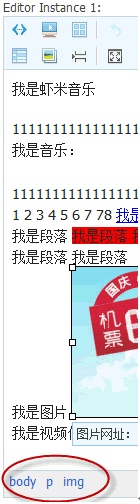
\includegraphics{elementpaths.png}
\end{quote}


\subparagraph{sourcearea}
\label{relatedproj/editorguide/plugin:sourcearea}\begin{quote}

点击后可以查看编辑器产生的html代码.


\includegraphics{sourcearea.png}
\end{quote}


\subparagraph{preview}
\label{relatedproj/editorguide/plugin:preview}\begin{quote}

点击后可以弹出新窗口, 查看编辑器的内容预览.


\includegraphics{preview.png}
\end{quote}


\subparagraph{templates}
\label{relatedproj/editorguide/plugin:templates}\begin{quote}

点击后可以弹出模板选择窗口, 选定后可以将模板代码插入到编辑器光标所在处.


\includegraphics{templates.png}
\end{quote}


\subparagraph{separator}
\label{relatedproj/editorguide/plugin:separator}\begin{quote}

间隔线.


\includegraphics{separator.png}
\end{quote}


\subparagraph{undo}
\label{relatedproj/editorguide/plugin:undo}\begin{quote}

可以撤销重做.


\includegraphics{undo.png}
\end{quote}


\subparagraph{removeformat}
\label{relatedproj/editorguide/plugin:removeformat}\begin{quote}

可以清除选择区域的编辑格式(字体, 大小, 加粗).


\includegraphics{removeformat.png}
\end{quote}


\subparagraph{font}
\label{relatedproj/editorguide/plugin:font}\begin{quote}

大小: 可以改变选择区域字体的大小.

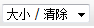
\includegraphics{fontsize.png}

字体: 可以改变选择区域的字体种类.

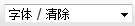
\includegraphics{fontfamily.png}

粗体: 可以将选择区域文字加粗.


\includegraphics{fontbold.png}

斜体: 可以将选择区域文字倾斜.


\includegraphics{fontitalic.png}

下划线: 可以给选择区域文字加下划线.


\includegraphics{fontunderline.png}

删除线: 可以给选择区域文字加删除线.


\includegraphics{fontdelete.png}
\end{quote}


\subparagraph{format}
\label{relatedproj/editorguide/plugin:format}\begin{quote}

可以将光标所在处块加入标题格式.

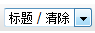
\includegraphics{format.png}
\end{quote}


\subparagraph{color}
\label{relatedproj/editorguide/plugin:color}\begin{quote}

设置选择区域的文本颜色.


\includegraphics{forecolor.png}

设置选择区域的背景颜色.


\includegraphics{bgcolor.png}
\end{quote}


\subparagraph{list}
\label{relatedproj/editorguide/plugin:list}\begin{quote}

为选择区域或光标所在处加上项目编号.


\includegraphics{list1.png}

为选择区域或光标所在处加上列表编号.


\includegraphics{list2.png}
\end{quote}


\subparagraph{indent}
\label{relatedproj/editorguide/plugin:indent}\begin{quote}

减少光标处的缩进量.


\includegraphics{indent1.png}

增加光标处的缩进量.


\includegraphics{indent2.png}
\end{quote}


\subparagraph{justify}
\label{relatedproj/editorguide/plugin:justify}\begin{quote}

左对齐: 光标所在块左对齐.


\includegraphics{justify1.png}

居中对齐: 光标所在块居中对齐.


\includegraphics{justify2.png}

右对齐: 光标所在块右对齐.


\includegraphics{justify3.png}
\end{quote}


\subparagraph{link}
\label{relatedproj/editorguide/plugin:link}\begin{quote}

编辑选择区域的超链接.


\includegraphics{link.png}
\end{quote}


\subparagraph{image}
\label{relatedproj/editorguide/plugin:image}\begin{quote}

输入图像地址将图像插入到光标所在处.


\includegraphics{image.png}
\end{quote}


\subparagraph{flash}
\label{relatedproj/editorguide/plugin:flash}\begin{quote}

输入flash地址将flash插入到光标所在处.


\includegraphics{flash.png}
\end{quote}


\subparagraph{music}
\label{relatedproj/editorguide/plugin:music}\begin{quote}

输入音乐地址将音乐插入到光标所在处.


\includegraphics{music.png}
\end{quote}


\subparagraph{smiley}
\label{relatedproj/editorguide/plugin:smiley}\begin{quote}

选择表情并将对应表情插入到光标所在处.


\includegraphics{smiley.png}
\end{quote}


\subparagraph{table}
\label{relatedproj/editorguide/plugin:table}\begin{quote}

输入表格相关参数并将对应表格插入到光标所在处.


\includegraphics{table.png}
\end{quote}


\subparagraph{resize}
\label{relatedproj/editorguide/plugin:resize}\begin{quote}

可拖动调整编辑区域大小.

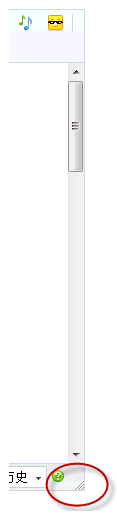
\includegraphics{resize.png}
\end{quote}


\subparagraph{pagebreak}
\label{relatedproj/editorguide/plugin:pagebreak}\begin{quote}

插入分页标记.

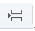
\includegraphics{pagebreak.png}
\end{quote}


\subparagraph{maximize}
\label{relatedproj/editorguide/plugin:maximize}\begin{quote}

将编辑器充满整个屏幕.


\includegraphics{maximize.png}
\end{quote}


\subparagraph{扩展插件}
\label{relatedproj/editorguide/plugin:id2}
如果要使用以下插件, 需要引入另外的 javascript 文件

\begin{Verbatim}[commandchars=\\\{\}]
\PYG{n+nt}{\textless{}script }\PYG{n+na}{src=}\PYG{l+s}{"http://a.tbcdn.cn/s/kissy/1.1.7/editor/biz/ext/editor-plugin-pkg-min.js"}\PYG{n+nt}{\textgreater{}}\PYG{n+nt}{\textless{}/script\textgreater{}}
\end{Verbatim}


\subparagraph{multi-upload}
\label{relatedproj/editorguide/plugin:multi-upload}\begin{quote}

多图同时上传功能


\includegraphics{mul-upload.png}

具体弹窗交互:

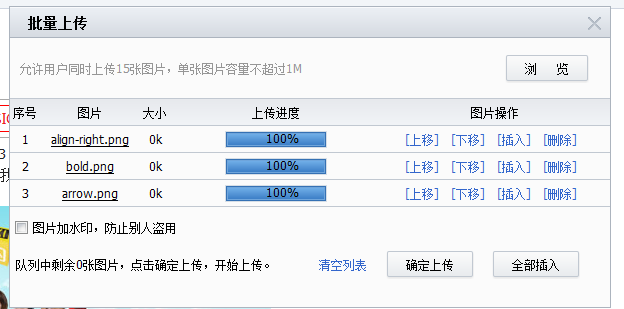
\includegraphics{mul-upload_win.png}
\end{quote}


\subparagraph{checkbox-sourcearea}
\label{relatedproj/editorguide/plugin:checkbox-sourcearea}\begin{quote}

勾选交互的源码切换功能

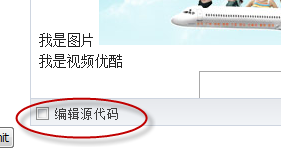
\includegraphics{checkbox-sourcearea.png}
\end{quote}


\subparagraph{video}
\label{relatedproj/editorguide/plugin:video}\begin{quote}

国内视频插入,方便直接输入url插入国内视频 flash


\includegraphics{video.png}

具体弹窗交互:

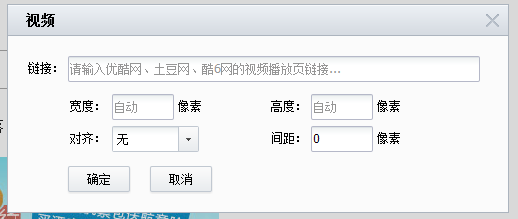
\includegraphics{video_win.png}
\end{quote}


\subparagraph{xiami-music}
\label{relatedproj/editorguide/plugin:xiami-music}\begin{quote}

虾米音乐插入,可通过搜索插入虾米音乐


\includegraphics{xiami.png}

具体弹窗交互:

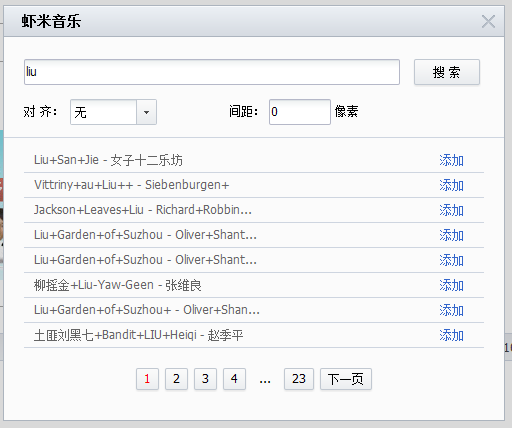
\includegraphics{xiami_win.png}
\end{quote}


\paragraph{插件配置}
\label{relatedproj/editorguide/plugin-config::doc}\label{relatedproj/editorguide/plugin-config:editorusage-common-cfg}\label{relatedproj/editorguide/plugin-config:id1}


\begin{fulllineitems}
\pysigline{\bfcode{config.pluginConfig:}}{}
类型为各个插件的具体配置, 配置形式为:

\begin{Verbatim}[commandchars=@\[\]]
{
        "插件名":插件配置
}
\end{Verbatim}

包括以下插件配置:

\index{link (Editor.pluginConfig attribute)}

\begin{fulllineitems}
\phantomsection\label{relatedproj/editorguide/plugin-config:Editor.pluginConfig.link}\pysigline{\code{pluginConfig.}\bfcode{link}}{}
超链接配置, 目前包括
\begin{quote}

\index{target (Editor.pluginConfig.link attribute)}

\begin{fulllineitems}
\phantomsection\label{relatedproj/editorguide/plugin-config:Editor.pluginConfig.link.target}\pysigline{\code{link.}\bfcode{target}}{}
默认为 ``'', 表示在当前窗口打开新链接, 也可以指定 ``\_blank'' , 则可以在新窗口打开链接. 例如

\begin{Verbatim}[commandchars=\\\{\}]
\PYG{n+nx}{pluginConfig} \PYG{o}{:} \PYG{p}{\PYGZob{}}
    \PYG{n+nx}{link}\PYG{o}{:}\PYG{p}{\PYGZob{}}
        \PYG{n+nx}{target}\PYG{o}{:}\PYG{l+s+s2}{"\PYGZus{}blank"}
    \PYG{p}{\PYGZcb{}}
\PYG{p}{\PYGZcb{}}
\end{Verbatim}

\end{fulllineitems}

\end{quote}

\end{fulllineitems}


\index{upload (Editor.pluginConfig.image attribute)}

\begin{fulllineitems}
\phantomsection\label{relatedproj/editorguide/plugin-config:Editor.pluginConfig.image.upload}\pysigline{\code{pluginConfig.image.}\bfcode{upload}}{}
上传图片配置, 不需要上传功能可不配置, 包括以下子配置
\begin{quote}

\index{serverUrl (Editor.pluginConfig.image.upload attribute)}

\begin{fulllineitems}
\phantomsection\label{relatedproj/editorguide/plugin-config:Editor.pluginConfig.image.upload.serverUrl}\pysigline{\code{upload.}\bfcode{serverUrl}}{}
接受文件数据的服务器端程序地址, 格式为 multipart/form-data , 返回格式为:
\begin{itemize}
\item {}
正确:\{``imgUrl'':''\href{http://xx.com/yy.jpg}{http://xx.com/yy.jpg}``\}

\item {}
错误:\{``error'':''i am error!''\}

\end{itemize}

\end{fulllineitems}


\index{serverParams (Editor.pluginConfig.image.upload attribute)}

\begin{fulllineitems}
\phantomsection\label{relatedproj/editorguide/plugin-config:Editor.pluginConfig.image.upload.serverParams}\pysigline{\code{upload.}\bfcode{serverParams}}{}
类型object, 键值对. 传给服务器的格外参数, 如果 value 是函数则传递函数执行结果

\end{fulllineitems}


\index{suffix (Editor.pluginConfig.image.upload attribute)}

\begin{fulllineitems}
\phantomsection\label{relatedproj/editorguide/plugin-config:Editor.pluginConfig.image.upload.suffix}\pysigline{\code{upload.}\bfcode{suffix}}{}
类型字符串, 允许图片的后缀名

\end{fulllineitems}


\index{fileInput (Editor.pluginConfig.image.upload attribute)}

\begin{fulllineitems}
\phantomsection\label{relatedproj/editorguide/plugin-config:Editor.pluginConfig.image.upload.fileInput}\pysigline{\code{upload.}\bfcode{fileInput}}{}
类型字符串, 传给服务器的文件域名

\end{fulllineitems}


\index{sizeLimit (Editor.pluginConfig.image.upload attribute)}

\begin{fulllineitems}
\phantomsection\label{relatedproj/editorguide/plugin-config:Editor.pluginConfig.image.upload.sizeLimit}\pysigline{\code{upload.}\bfcode{sizeLimit}}{}
类型整数, 限制上传的文件大小, 单位 KB, ie 下只能作为提示.

\end{fulllineitems}


\index{extraHtml (Editor.pluginConfig.image.upload attribute)}

\begin{fulllineitems}
\phantomsection\label{relatedproj/editorguide/plugin-config:Editor.pluginConfig.image.upload.extraHtml}\pysigline{\code{upload.}\bfcode{extraHtml}}{}
放入图片上传区域的其他 html

\end{fulllineitems}

\end{quote}

例如:

\begin{Verbatim}[commandchars=\\\{\}]
\PYG{n+nx}{pluginConfig}\PYG{o}{:} \PYG{p}{\PYGZob{}}
    \PYG{c+c1}{// 图片插件配置}
    \PYG{l+s+s2}{"image"}\PYG{o}{:} \PYG{p}{\PYGZob{}}
        \PYG{c+c1}{//上传图片配置, 不需要上传功能可不配置}
        \PYG{n+nx}{upload}\PYG{o}{:} \PYG{p}{\PYGZob{}}
            \PYG{c+c1}{//返回格式}
            \PYG{c+c1}{//正确:\PYGZob{}"imgUrl":"http://xx.com/yy.jpg"\PYGZcb{}}
            \PYG{c+c1}{//错误:\PYGZob{}"error":"i am error!"\PYGZcb{}}
            \PYG{c+c1}{//接受图片的服务器}
            \PYG{c+c1}{//发送一个文件过去, 格式为 multipart/form-data}
            \PYG{n+nx}{serverUrl}\PYG{o}{:} \PYG{l+s+s2}{"/code/upload/upload.jsp"}\PYG{p}{,}
            \PYG{c+c1}{//传给服务器的格外参数, 是函数则传递函数执行结果}
            \PYG{n+nx}{serverParams}\PYG{o}{:} \PYG{p}{\PYGZob{}}
                \PYG{n+nx}{yy}\PYG{o}{:} \PYG{k+kd}{function} \PYG{p}{(}\PYG{p}{)} \PYG{p}{\PYGZob{}}
                    \PYG{k}{return} \PYG{l+s+s2}{"xx"}\PYG{p}{;}
                \PYG{p}{\PYGZcb{}}
            \PYG{p}{\PYGZcb{}}\PYG{p}{,}
            \PYG{c+c1}{//后缀名白名单}
            \PYG{n+nx}{suffix}\PYG{o}{:} \PYG{l+s+s2}{"png,jpg,jpeg,gif"}\PYG{p}{,}
            \PYG{c+c1}{//传递给server的文件域名字}
            \PYG{n+nx}{fileInput}\PYG{o}{:} \PYG{l+s+s2}{"Filedata"}\PYG{p}{,}
            \PYG{c+c1}{//限制上传的文件大小, 单位KB,}
            \PYG{c+c1}{//无法客户端限制, 只能作为提示信息}
            \PYG{n+nx}{sizeLimit}\PYG{o}{:} \PYG{l+m+mi}{1000}\PYG{p}{,}
            \PYG{c+c1}{//k}
            \PYG{c+c1}{//自己想要添加的其他输入域}
            \PYG{n+nx}{extraHtml}\PYG{o}{:} \PYG{l+s+s2}{"\textless{}p style='margin-top:5px;'\textgreater{}"} \PYG{o}{+} \PYG{l+s+s2}{"\textless{}input type='checkbox' name='ke\PYGZus{}img\PYGZus{}up\PYGZus{}watermark\PYGZus{}1'\textgreater{} 图片加水印, 防止别人盗用\textless{}/p\textgreater{}"}
        \PYG{p}{\PYGZcb{}}
    \PYG{p}{\PYGZcb{}}
\PYG{p}{\PYGZcb{}}
\end{Verbatim}

\begin{notice}{note}{Note:}
如果页面中设置了 document.domain='xx.com', 那么这时上传图片服务器要返回一段设置 domain 的 html, 例如

\begin{Verbatim}[commandchars=\\\{\}]
\PYG{n+nt}{\textless{}html}\PYG{n+nt}{\textgreater{}}
    \PYG{n+nt}{\textless{}head}\PYG{n+nt}{\textgreater{}}
        \PYG{n+nt}{\textless{}script}\PYG{n+nt}{\textgreater{}}
            \PYG{n+nb}{document}\PYG{p}{.}\PYG{n+nx}{domain}\PYG{o}{=}\PYG{l+s+s2}{"xx.com"}\PYG{p}{;}
        \PYG{n+nt}{\textless{}/script\textgreater{}}
    \PYG{n+nt}{\textless{}/head\textgreater{}}
    \PYG{n+nt}{\textless{}body}\PYG{n+nt}{\textgreater{}}
        \PYGZob{}"imgUrl":"http://img03.taobaocdn.com/sns\PYGZus{}album/i3/T13fhRXftcXXb1upjX.jpg"\PYGZcb{}
    \PYG{n+nt}{\textless{}/body\textgreater{}}
\PYG{n+nt}{\textless{}/html\textgreater{}}
\end{Verbatim}
\end{notice}

\end{fulllineitems}


\index{templates (Editor.pluginConfig attribute)}

\begin{fulllineitems}
\phantomsection\label{relatedproj/editorguide/plugin-config:Editor.pluginConfig.templates}\pysigline{\code{pluginConfig.}\bfcode{templates}}{}
模板 (templates) 配置, 类型数组, 数组每个元素为单个模板的配置, 单个配置包括
\begin{quote}

\index{demo (Editor.pluginConfig.templates attribute)}

\begin{fulllineitems}
\phantomsection\label{relatedproj/editorguide/plugin-config:Editor.pluginConfig.templates.demo}\pysigline{\code{templates.}\bfcode{demo}}{}
类型字符串, 模板的简单介绍

\end{fulllineitems}


\index{html (Editor.pluginConfig.templates attribute)}

\begin{fulllineitems}
\phantomsection\label{relatedproj/editorguide/plugin-config:Editor.pluginConfig.templates.html}\pysigline{\code{templates.}\bfcode{html}}{}
类型字符串, 将要插入到编辑器区域的具体内容

\end{fulllineitems}

\end{quote}

例如:

\begin{Verbatim}[commandchars=\\\{\}]
\PYG{p}{\PYGZob{}}
    \PYG{l+s+s2}{"templates"}\PYG{o}{:} \PYG{p}{[}\PYG{p}{\PYGZob{}}
        \PYG{c+c1}{//显示模板的简单介绍}
        \PYG{n+nx}{demo}\PYG{o}{:} \PYG{l+s+s2}{"模板1效果演示html"}\PYG{p}{,}
        \PYG{c+c1}{//插入到编辑器区域的具体内容}
        \PYG{n+nx}{html}\PYG{o}{:} \PYG{l+s+s2}{"\textless{}div style='border:1px solid red'\textgreater{}模板1效果演示html\textless{}/div\textgreater{}\textless{}p\textgreater{}\textless{}/p\textgreater{}"}
    \PYG{p}{\PYGZcb{}}\PYG{p}{,}
    \PYG{p}{\PYGZob{}}
        \PYG{n+nx}{demo}\PYG{o}{:} \PYG{l+s+s2}{"模板2效果演示html"}\PYG{p}{,}
        \PYG{n+nx}{html}\PYG{o}{:} \PYG{l+s+s2}{"\textless{}div style='border:1px solid red'\textgreater{}模板2效果演示html\textless{}/div\textgreater{}"}
    \PYG{p}{\PYGZcb{}}\PYG{p}{]}\PYG{p}{,}
\PYG{p}{\PYGZcb{}}
\end{Verbatim}

\end{fulllineitems}




\begin{fulllineitems}
\pysigline{\bfcode{pluginConfig.font-size}}{}
字体大小配置, 类型 object 或 boolean. 当为 false 时, 则该按钮不出现在编辑器中. 当为 object 时, 包含子配置
\begin{quote}



\begin{fulllineitems}
\pysigline{\bfcode{font-size.items}}{}
类型对象数组, 数组每一项的配置为:
\begin{quote}

\index{value (Editor.items attribute)}

\begin{fulllineitems}
\phantomsection\label{relatedproj/editorguide/plugin-config:Editor.items.value}\pysigline{\code{items.}\bfcode{value}}{}
类型 string, 真实的字体大小

\end{fulllineitems}


\index{attrs (Editor.items attribute)}

\begin{fulllineitems}
\phantomsection\label{relatedproj/editorguide/plugin-config:Editor.items.attrs}\pysigline{\code{items.}\bfcode{attrs}}{}
类型 object, 键值对添加到每个字体的对应节点上

\end{fulllineitems}


\index{name (Editor.items attribute)}

\begin{fulllineitems}
\phantomsection\label{relatedproj/editorguide/plugin-config:Editor.items.name}\pysigline{\code{items.}\bfcode{name}}{}
类型 string, 字体大小的显示值

\end{fulllineitems}

\end{quote}

\end{fulllineitems}

\end{quote}

例如:

\begin{Verbatim}[commandchars=\\\{\}]
\PYG{p}{\PYGZob{}}
    \PYG{l+s+s2}{"font-size"}\PYG{o}{:} \PYG{p}{\PYGZob{}}
        \PYG{c+c1}{//字体大小下拉框的配置}
        \PYG{n+nx}{items}\PYG{o}{:} \PYG{p}{[}\PYG{p}{\PYGZob{}}
            \PYG{c+c1}{//真实的字体大小值}
            \PYG{n+nx}{value}\PYG{o}{:} \PYG{l+s+s2}{"14px"}\PYG{p}{,}
            \PYG{c+c1}{//字体大小选项框样式, 可不配置}
            \PYG{n+nx}{attrs}\PYG{o}{:} \PYG{p}{\PYGZob{}}
                \PYG{n+nx}{style}\PYG{o}{:} \PYG{l+s+s1}{'position: relative; border: 1px solid \#DDDDDD; margin: 2px; padding: 2px;'}
            \PYG{p}{\PYGZcb{}}\PYG{p}{,}
            \PYG{c+c1}{//单个字体大小的显示值}
            \PYG{n+nx}{name}\PYG{o}{:} \PYG{l+s+s2}{" \textless{}span style='font-size:14px'\textgreater{}标准\textless{}/span\textgreater{}"} \PYG{o}{+} \PYG{l+s+s2}{"\textless{}span style='position:absolute;top:1px;right:3px;'\textgreater{}14px\textless{}/span\textgreater{}"}
        \PYG{p}{\PYGZcb{}}\PYG{p}{]}
    \PYG{p}{\PYGZcb{}}

\PYG{p}{\PYGZcb{}}
\end{Verbatim}

\end{fulllineitems}




\begin{fulllineitems}
\pysigline{\bfcode{pluginConfig.font-family}}{}
字体种类配置, 类型 object, 包含子配置项
\begin{quote}



\begin{fulllineitems}
\pysigline{\bfcode{font-family.items}}{}
类型对象数组, 字体种类配置, 单个配置包含
\begin{quote}

\index{name (Editor.items attribute)}

\begin{fulllineitems}
\pysigline{\code{items.}\bfcode{name}}{}
字体显示值

\end{fulllineitems}


\index{value (Editor.items attribute)}

\begin{fulllineitems}
\pysigline{\code{items.}\bfcode{value}}{}
设置到编辑元素的真实值

\end{fulllineitems}

\end{quote}

\end{fulllineitems}

\end{quote}

例如:

\begin{Verbatim}[commandchars=\\\{\}]
\PYG{p}{\PYGZob{}}
    \PYG{l+s+s2}{"font-family"}\PYG{o}{:} \PYG{p}{\PYGZob{}}
        \PYG{n+nx}{items}\PYG{o}{:} \PYG{p}{[}\PYG{p}{\PYGZob{}}
            \PYG{c+c1}{//显示值}
            \PYG{n+nx}{name}\PYG{o}{:} \PYG{l+s+s2}{"宋体"}\PYG{p}{,}
            \PYG{c+c1}{//真实值}
            \PYG{n+nx}{value}\PYG{o}{:} \PYG{l+s+s2}{"SimSun"}
        \PYG{p}{\PYGZcb{}}\PYG{p}{,}
        \PYG{p}{\PYGZob{}}
            \PYG{n+nx}{name}\PYG{o}{:} \PYG{l+s+s2}{"黑体"}\PYG{p}{,}
            \PYG{n+nx}{value}\PYG{o}{:} \PYG{l+s+s2}{"SimHei"}
        \PYG{p}{\PYGZcb{}}\PYG{p}{]}
    \PYG{p}{\PYGZcb{}}
\PYG{p}{\PYGZcb{}}
\end{Verbatim}

\end{fulllineitems}




\begin{fulllineitems}
\pysigline{\bfcode{pluginConfig.font-bold}}{}
是否显示粗体按钮, 默认 true

\end{fulllineitems}




\begin{fulllineitems}
\pysigline{\bfcode{pluginConfig.font-italic}}{}
是否显示斜体按钮, 默认 true

\end{fulllineitems}




\begin{fulllineitems}
\pysigline{\bfcode{pluginConfig.font-underline}}{}
是否显示下划线按钮, 默认 true

\end{fulllineitems}




\begin{fulllineitems}
\pysigline{\bfcode{pluginConfig.font-strikeThrough}}{}
是否显示删除线按钮, 默认 true

\end{fulllineitems}


\index{draft (Editor.pluginConfig attribute)}

\begin{fulllineitems}
\phantomsection\label{relatedproj/editorguide/plugin-config:Editor.pluginConfig.draft}\pysigline{\code{pluginConfig.}\bfcode{draft}}{}
草稿箱

例如

\begin{Verbatim}[commandchars=\\\{\}]
\PYG{p}{\PYGZob{}}
    \PYG{l+s+s2}{"draft"}\PYG{o}{:} \PYG{p}{\PYGZob{}}
        \PYG{c+c1}{//分钟设置:每隔几分钟保存一次}
        \PYG{n+nx}{interval}\PYG{o}{:} \PYG{l+m+mi}{5}\PYG{p}{,}
        \PYG{c+c1}{//最多保存几条历史记录?}
        \PYG{n+nx}{limit}\PYG{o}{:} \PYG{l+m+mi}{10}\PYG{p}{,}
        \PYG{c+c1}{//草稿箱帮助文案, 可不设置}
        \PYG{n+nx}{helpHtml}\PYG{o}{:} \PYG{l+s+s2}{"\textless{}div "} \PYG{o}{+} \PYG{l+s+s2}{"style='width:200px;'\textgreater{}"} \PYG{o}{+} \PYG{l+s+s2}{"\textless{}div style='padding:5px;'\textgreater{}草稿箱能够自动保存您最新编辑的内容, "} \PYG{o}{+} \PYG{l+s+s2}{"如果发现内容丢失, "} \PYG{o}{+} \PYG{l+s+s2}{"请选择恢复编辑历史\textless{}/div\textgreater{}\textless{}/div\textgreater{}"}
    \PYG{p}{\PYGZcb{}}
\PYG{p}{\PYGZcb{}}
\end{Verbatim}

\end{fulllineitems}


\index{resize (Editor.pluginConfig attribute)}

\begin{fulllineitems}
\phantomsection\label{relatedproj/editorguide/plugin-config:Editor.pluginConfig.resize}\pysigline{\code{pluginConfig.}\bfcode{resize}}{}
右下角调整大小的配置

例如

\begin{Verbatim}[commandchars=\\\{\}]
\PYG{p}{\PYGZob{}}
    \PYG{l+s+s2}{"resize"}\PYG{o}{:} \PYG{p}{\PYGZob{}}
        \PYG{c+c1}{//只能在y轴拖放, [“x”,”y”]表示任意拖放}
        \PYG{n+nx}{direction}\PYG{o}{:} \PYG{p}{[}\PYG{l+s+s2}{"y"}\PYG{p}{]}
    \PYG{p}{\PYGZcb{}}
\PYG{p}{\PYGZcb{}}
\end{Verbatim}

\end{fulllineitems}


\index{music (Editor.pluginConfig attribute)}

\begin{fulllineitems}
\phantomsection\label{relatedproj/editorguide/plugin-config:Editor.pluginConfig.music}\pysigline{\code{pluginConfig.}\bfcode{music}}{}
音乐插件配置, 支持音乐文件地址输入, 直接播放mp3

例如:

\begin{Verbatim}[commandchars=\\\{\}]
\PYG{n+nx}{music}\PYG{o}{:} \PYG{p}{\PYGZob{}}
    \PYG{c+c1}{//必须和网址url同域而不是类库同域}
    \PYG{n+nx}{musicPlayer}\PYG{o}{:} \PYG{l+s+s2}{"/music/niftyplayer.swf"}
\PYG{p}{\PYGZcb{}}
\end{Verbatim}

\end{fulllineitems}




\begin{fulllineitems}
\pysigline{\bfcode{pluginConfig.multi-upload}}{}
图片批量上传

例如

\begin{Verbatim}[commandchars=\\\{\}]
\PYG{p}{\PYGZob{}}
    \PYG{l+s+s2}{"multi-upload"}\PYG{o}{:} \PYG{p}{\PYGZob{}}
        \PYG{c+c1}{//同图片上传插件配置}
        \PYG{c+c1}{//返回格式}
        \PYG{c+c1}{//正确:\PYGZob{}"imgUrl":""\PYGZcb{}}
        \PYG{c+c1}{//错误:\PYGZob{}"error":""\PYGZcb{}}
        \PYG{c+c1}{//注意:中文 \PYGZbs{}uxxxx 转义}
        \PYG{c+c1}{//发送一个文件过去, 格式为 multipart/form-data}
        \PYG{c+c1}{//接受图片的服务器, 注意必须绝对地址}
        \PYG{n+nx}{serverUrl}\PYG{o}{:} \PYG{l+s+s2}{"http://xx.com/code/upload/upload.jsp"}\PYG{p}{,}
        \PYG{c+c1}{//同图片配置}
        \PYG{n+nx}{serverParams}\PYG{o}{:} \PYG{p}{\PYGZob{}}
            \PYG{n+nx}{waterMark}\PYG{o}{:} \PYG{k+kd}{function} \PYG{p}{(}\PYG{p}{)} \PYG{p}{\PYGZob{}}
                \PYG{k}{return} \PYG{n+nx}{S}\PYG{p}{.}\PYG{n+nx}{one}\PYG{p}{(}\PYG{l+s+s2}{"\#ke\PYGZus{}img\PYGZus{}up\PYGZus{}watermark\PYGZus{}2"}\PYG{p}{)}\PYG{p}{[}\PYG{l+m+mi}{0}\PYG{p}{]}\PYG{p}{.}\PYG{n+nx}{checked}\PYG{p}{;}
            \PYG{p}{\PYGZcb{}}
        \PYG{p}{\PYGZcb{}}\PYG{p}{,}
        \PYG{c+c1}{//同图片配置}
        \PYG{n+nx}{extraHtml}\PYG{o}{:} \PYG{l+s+s2}{"\textless{}p style='margin-top:10px;'\textgreater{}"} \PYG{o}{+} \PYG{l+s+s2}{"\textless{}input type='checkbox' "} \PYG{o}{+} \PYG{l+s+s2}{"style='vertical-align:middle;margin:0 5px;' "} \PYG{o}{+} \PYG{l+s+s2}{"id='ke\PYGZus{}img\PYGZus{}up\PYGZus{}watermark\PYGZus{}2'\textgreater{}"} \PYG{o}{+} \PYG{l+s+s2}{"\textless{}span style='vertical-align:middle;'\textgreater{}图片加水印, 防止别人盗用\textless{}/span\textgreater{}\textless{}/p\textgreater{}"}\PYG{p}{,}
        \PYG{c+c1}{//缩略图的后缀名}
        \PYG{c+c1}{//原图:http://xx.com/yy.jpg}
        \PYG{c+c1}{//则加入后缀名时变为:}
        \PYG{c+c1}{//http://xx.com/yy\PYGZus{}80x80.jpg}
        \PYG{n+nx}{previewSuffix}\PYG{o}{:} \PYG{l+s+s2}{"\PYGZus{}80x80"}\PYG{p}{,}

        \PYG{c+c1}{//缩略图窗口宽度, 高度根据图片自适应}
        \PYG{c+c1}{//若不需要缩略图功能, 不配置即可}
        \PYG{n+nx}{previewWidth}\PYG{o}{:} \PYG{l+s+s2}{"80px"}\PYG{p}{,}

        \PYG{c+c1}{//客户端 flash 验证}
        \PYG{n+nx}{sizeLimit}\PYG{o}{:} \PYG{l+m+mi}{1000} \PYG{c+c1}{//k,}
        \PYG{c+c1}{//新增配置:可同时显示的图片列表个数}
        \PYG{n+nx}{numberLimit}\PYG{o}{:} \PYG{l+m+mi}{15}
    \PYG{p}{\PYGZcb{}}
\PYG{p}{\PYGZcb{}}
\end{Verbatim}

\begin{notice}{note}{Note:}
\#.该插件使用 flash 技术, 必须在根域名下提供 crossdomain.xml , 例如 \href{http://www.taobao.com/crossdomain.xml}{http://www.taobao.com/crossdomain.xml} , 内容如下

\begin{Verbatim}[commandchars=\\\{\}]
\PYG{n+nt}{\textless{}cross-domain-policy}\PYG{n+nt}{\textgreater{}}
    \PYG{n+nt}{\textless{}allow-access-from} \PYG{n+na}{domain=}\PYG{l+s}{"*.taobao.com"}\PYG{n+nt}{/\textgreater{}}
    \PYG{n+nt}{\textless{}allow-access-from} \PYG{n+na}{domain=}\PYG{l+s}{"*.taobao.net"}\PYG{n+nt}{/\textgreater{}}
    \PYG{n+nt}{\textless{}allow-access-from} \PYG{n+na}{domain=}\PYG{l+s}{"*.taobaocdn.com"}\PYG{n+nt}{/\textgreater{}}
    \PYG{n+nt}{\textless{}allow-access-from} \PYG{n+na}{domain=}\PYG{l+s}{"*.tbcdn.cn"}\PYG{n+nt}{/\textgreater{}}
    \PYG{n+nt}{\textless{}allow-access-from} \PYG{n+na}{domain=}\PYG{l+s}{"*.allyes.com"}\PYG{n+nt}{/\textgreater{}}
\PYG{n+nt}{\textless{}/cross-domain-policy\textgreater{}}
\end{Verbatim}

\#.serverUrl 必须使用绝对地址, 否则如果编辑器组件和应用页面不在同一个hostname时, firefox下请求会发到编辑器组件所在的hostname.
\end{notice}

\end{fulllineitems}


\index{video (Editor.pluginConfig attribute)}

\begin{fulllineitems}
\phantomsection\label{relatedproj/editorguide/plugin-config:Editor.pluginConfig.video}\pysigline{\code{pluginConfig.}\bfcode{video}}{}
国内视频插入, 可直接输入tudou,youku,ku6的url进行视频粘贴.

例如:

\begin{Verbatim}[commandchars=\\\{\}]
\PYG{p}{\PYGZob{}}
    \PYG{l+s+s2}{"video"}\PYG{o}{:} \PYG{p}{\PYGZob{}}
        \PYG{n+nx}{urlCfg}\PYG{o}{:} \PYG{p}{[}\PYG{p}{\PYGZob{}}
            \PYG{n+nx}{reg}\PYG{o}{:} \PYG{l+s+sr}{/tudou\PYGZbs{}.com/i}\PYG{p}{,}
            \PYG{c+c1}{//地址配置后端咨询:石冲}
            \PYG{n+nx}{url}\PYG{o}{:} \PYG{l+s+s2}{"http://bangpai.daily.taobao.net/json/getTudouVideo.htm?"} \PYG{o}{+} \PYG{l+s+s2}{"url=@url@\&callback=@callback@"}
        \PYG{p}{\PYGZcb{}}\PYG{p}{]}\PYG{p}{,}
        \PYG{c+c1}{//输入框提示信息}
        \PYG{n+nx}{urlTip}\PYG{o}{:} \PYG{l+s+s2}{"请输入优酷网、土豆网、酷7网的视频播放页链接..."}\PYG{p}{,}
        \PYG{c+c1}{//静态转换规则, 从用户输入转换为flash地址, 例如优酷:}
        \PYG{n+nx}{providers}\PYG{o}{:} \PYG{p}{[}\PYG{p}{\PYGZob{}}
            \PYG{n+nx}{reg}\PYG{o}{:} \PYG{l+s+sr}{/youku\PYGZbs{}.com/i}\PYG{p}{,}
            \PYG{n+nx}{width}\PYG{o}{:} \PYG{l+m+mi}{480}\PYG{p}{,}
            \PYG{n+nx}{height}\PYG{o}{:} \PYG{l+m+mi}{400}\PYG{p}{,}
            \PYG{n+nx}{detect}\PYG{o}{:} \PYG{k+kd}{function} \PYG{p}{(}\PYG{n+nx}{url}\PYG{p}{)} \PYG{p}{\PYGZob{}}
                \PYG{k+kd}{var} \PYG{n+nx}{m} \PYG{o}{=} \PYG{n+nx}{url}\PYG{p}{.}\PYG{n+nx}{match}\PYG{p}{(}\PYG{l+s+sr}{/id\PYGZus{}([\PYGZca{}.]+)\PYGZbs{}.html\$/}\PYG{p}{)}\PYG{p}{;}
                \PYG{k}{if} \PYG{p}{(}\PYG{n+nx}{m}\PYG{p}{)} \PYG{p}{\PYGZob{}}
                    \PYG{k}{return} \PYG{l+s+s2}{"http://player.youku.com/player.php/sid/"} \PYG{o}{+} \PYG{n+nx}{m}\PYG{p}{[}\PYG{l+m+mi}{1}\PYG{p}{]} \PYG{o}{+} \PYG{l+s+s2}{"/v.swf"}\PYG{p}{;}
                \PYG{p}{\PYGZcb{}}
                \PYG{n+nx}{m} \PYG{o}{=} \PYG{n+nx}{url}\PYG{p}{.}\PYG{n+nx}{match}\PYG{p}{(}\PYG{l+s+sr}{/v\PYGZus{}playlist\PYGZbs{}/([\PYGZca{}.]+)\PYGZbs{}.html\$/}\PYG{p}{)}\PYG{p}{;}
                \PYG{k}{if} \PYG{p}{(}\PYG{n+nx}{m}\PYG{p}{)} \PYG{p}{\PYGZob{}}
                    \PYG{k}{return}\PYG{p}{;}
                    \PYG{c+c1}{//return "http://player.youku.com/player.php/sid/" + m[1] + "/v.swf";}
                \PYG{p}{\PYGZcb{}}
                \PYG{k}{return} \PYG{n+nx}{url}\PYG{p}{;}
            \PYG{p}{\PYGZcb{}}
        \PYG{p}{\PYGZcb{}}\PYG{p}{]}
    \PYG{p}{\PYGZcb{}}
\PYG{p}{\PYGZcb{}}
\end{Verbatim}

\end{fulllineitems}




\begin{fulllineitems}
\pysigline{\bfcode{pluginConfig.xiami-music}}{}
虾米音乐插入, 无需配置, 只要 use 即可.

\end{fulllineitems}


\end{fulllineitems}


\begin{notice}{note}{Note:}
xiami-music , video , multi-upload 为扩展插件, 若需要使用请引入外部js

\begin{Verbatim}[commandchars=\\\{\}]
\PYG{n+nt}{\textless{}script }\PYG{n+na}{src=}\PYG{l+s}{"http://a.tbcdn.cn/s/kissy/1.1.x/editor/biz/ext/editor-plugin-pkg-min.js"}\PYG{n+nt}{\textgreater{}}\PYG{n+nt}{\textless{}/script\textgreater{}}
\end{Verbatim}
\end{notice}


\subsubsection{注意}
\label{relatedproj/editorguide/notice:editorusage-notice}\label{relatedproj/editorguide/notice::doc}\label{relatedproj/editorguide/notice:id1}

\paragraph{应用样式}
\label{relatedproj/editorguide/notice:id2}
展示页面同样需要引入编辑器外部样式 :

\begin{Verbatim}[commandchars=\\\{\}]
\PYG{c}{\textless{}!--}\PYG{c}{[if lt IE 8]\textgreater{}}
\PYG{c}{\textless{}link href="http://a.tbcdn.cn/s/kissy/1.1.7/editor/theme/cool/editor}\PYG{c}{-}\PYG{c}{pkg}\PYG{c}{-}\PYG{c}{min}\PYG{c}{-}\PYG{c}{mhtml.css" rel="stylesheet"/\textgreater{}}
\PYG{c}{\textless{}![endif]}\PYG{c}{--\textgreater{}}
\PYG{c}{\textless{}!--}\PYG{c}{[if gte IE 8]\textgreater{}\textless{}!}\PYG{c}{--\textgreater{}}
\PYG{n+nt}{\textless{}link} \PYG{n+na}{href=}\PYG{l+s}{"http://a.tbcdn.cn/s/kissy/1.1.7/editor/theme/cool/editor-pkg-min-datauri.css"} \PYG{n+na}{rel=}\PYG{l+s}{"stylesheet"}\PYG{n+nt}{/\textgreater{}}
\PYG{c}{\textless{}!--}\PYG{c}{\textless{}![endif]}\PYG{c}{--\textgreater{}}
\end{Verbatim}

并且将从数据库中得到的编辑器生成内容用

\code{\textless{}div class="ke-post"\textgreater{}\textless{}/div\textgreater{}}

包裹起来.

如果使用了 {\hyperref[relatedproj/editorguide/plugin-config:editorusage-common-cfg]{\emph{一般配置中的自定义样式}}} ,
则需要在展示页面编辑器外部样式后重新定义你的自定义样式:

\begin{Verbatim}[commandchars=\\\{\}]
\PYG{n+nt}{\textless{}style }\PYG{n+na}{type=}\PYG{l+s}{"text/css"}\PYG{n+nt}{\textgreater{}}
    \PYG{n+nc}{.ke-post} \PYG{n+nt}{p} \PYG{p}{\PYGZob{}}
        \PYG{k}{color}\PYG{o}{:}\PYG{n+nb}{red}\PYG{p}{;}
    \PYG{p}{\PYGZcb{}}
\PYG{n+nt}{\textless{}/style\textgreater{}}
\end{Verbatim}


\paragraph{后端开发人员必看}
\label{relatedproj/editorguide/notice:id3}
\href{http://dev.taobao.net/?p=4033}{http://dev.taobao.net/?p=4033}


\subsubsection{FAQ}
\label{relatedproj/editorguide/faq:faq}\label{relatedproj/editorguide/faq::doc}

\paragraph{数据同步}
\label{relatedproj/editorguide/faq:id1}

\subparagraph{form 同步}
\label{relatedproj/editorguide/faq:form}\begin{quote}

如果后端通过 form 提交(submit)来获得用户输入数据, 则只需配置参数 {\hyperref[relatedproj/editorguide/usage:Editor.KISSY.Editor]{\code{attachForm}}}  .

\begin{Verbatim}[commandchars=\\\{\}]
\PYG{c+c1}{//是否监控编辑器所属的表单提交}
\PYG{l+s+s2}{"attachForm"}\PYG{o}{:}\PYG{k+kc}{true}\PYG{p}{,}
\end{Verbatim}

编辑器自动会监控 form 的 sbumit 事件进行同步
\end{quote}


\subparagraph{手动同步}
\label{relatedproj/editorguide/faq:id2}\begin{quote}

涉及三个 api

editor 为调用 KISSY.Editor 返回的编辑器实例

\code{editor.sync()} : 手动同步编辑器内容到对应 textarea

\code{editor.getData()} : 获得当前编辑器的内容

\code{editor.setData(html:string)} :设置当前编辑器的内容, 参数为html, 类型为 string 字符串
\end{quote}


\paragraph{自动保存}
\label{relatedproj/editorguide/faq:id3}\begin{quote}

自动保存为 localStorage/flash 机制, 保存在本地, 可 {\hyperref[relatedproj/editorguide/plugin-config:Editor.pluginConfig.draft]{\code{配置参数}}} .
\end{quote}


\paragraph{字数统计}
\label{relatedproj/editorguide/faq:id4}\begin{quote}

可参考以下 demo  :

\href{http://docs.kissyui.com/kissy-editor/demo/cdn/1.1.7/wordCount.html}{http://docs.kissyui.com/kissy-editor/demo/cdn/1.1.7/wordCount.html}

其中 \href{http://docs.kissyui.com/kissy-editor/demo/word-count.js}{wordcount 代码} 自行下载, 随意修改.
\end{quote}


\paragraph{绑定 ctrol-enter}
\label{relatedproj/editorguide/faq:ctrol-enter}
不少的应用场景要求在编辑器编辑区域内按下 ctrol+enter 按键时, 编辑器所在表单会自动提交, 解决方案是监控编辑器的文档按键事件:

\begin{Verbatim}[commandchars=\\\{\}]
\PYG{n+nx}{editor}\PYG{p}{.}\PYG{n+nx}{ready}\PYG{p}{(}\PYG{k+kd}{function} \PYG{p}{(}\PYG{p}{)} \PYG{p}{\PYGZob{}}
    \PYG{n+nx}{KISSY}\PYG{p}{.}\PYG{n+nx}{Event}\PYG{p}{.}\PYG{n+nx}{on}\PYG{p}{(}\PYG{n+nx}{editor}\PYG{p}{.}\PYG{n+nb}{document}\PYG{p}{,} \PYG{l+s+s2}{"keydown"}\PYG{p}{,} \PYG{k+kd}{function} \PYG{p}{(}\PYG{n+nx}{ev}\PYG{p}{)} \PYG{p}{\PYGZob{}}
        \PYG{k}{if} \PYG{p}{(}\PYG{n+nx}{ev}\PYG{p}{.}\PYG{n+nx}{keyCode} \PYG{o}{==} \PYG{l+m+mi}{13} \PYG{o}{\&\&} \PYG{n+nx}{ev}\PYG{p}{.}\PYG{n+nx}{ctrlKey}\PYG{p}{)} \PYG{p}{\PYGZob{}}
            \PYG{n+nx}{editor}\PYG{p}{.}\PYG{n+nx}{sync}\PYG{p}{(}\PYG{p}{)}\PYG{p}{;}
            \PYG{n+nx}{editor}\PYG{p}{.}\PYG{n+nx}{textarea}\PYG{p}{[}\PYG{l+m+mi}{0}\PYG{p}{]}\PYG{p}{.}\PYG{n+nx}{form}\PYG{p}{.}\PYG{n+nx}{submit}\PYG{p}{(}\PYG{p}{)}\PYG{p}{;}

        \PYG{p}{\PYGZcb{}}
    \PYG{p}{\PYGZcb{}}\PYG{p}{)}
\PYG{p}{\PYGZcb{}}\PYG{p}{)}\PYG{p}{;}
\end{Verbatim}

其中 editor 为编辑器实例的对象, 通过 \code{var editor=KISSY.Editor("\#id",cfg)} 获取而来.


\paragraph{placeholder(tip) 功能}
\label{relatedproj/editorguide/faq:placeholder-tip}\begin{quote}

可参考以下 demo  :

\href{http://docs.kissyui.com/kissy-editor/demo/cdn/1.1.7/tip.html}{http://docs.kissyui.com/kissy-editor/demo/cdn/1.1.7/tip.html}

其中 \href{http://docs.kissyui.com/kissy-editor/demo/tip.js}{tip 代码} 自行下载,随意修改。
\end{quote}


\paragraph{截获 paste 事件}
\label{relatedproj/editorguide/faq:paste}
可以通过监听编辑器实例对象的 ``paste'' 事件来截获用户粘贴的内容

\begin{Verbatim}[commandchars=\\\{\}]
\PYG{k+kd}{var} \PYG{n+nx}{editor}\PYG{o}{=}\PYG{n+nx}{KISSY}\PYG{p}{.}\PYG{n+nx}{Editor}\PYG{p}{(}\PYG{p}{.}\PYG{p}{.}\PYG{p}{)}\PYG{p}{;}
\PYG{n+nx}{editor}\PYG{p}{.}\PYG{n+nx}{on}\PYG{p}{(}\PYG{l+s+s2}{"paste"}\PYG{p}{,}\PYG{k+kd}{function}\PYG{p}{(}\PYG{n+nx}{ev}\PYG{p}{)}\PYG{p}{\PYGZob{}}
    \PYG{k+kd}{var} \PYG{n+nx}{html}\PYG{o}{=}\PYG{n+nx}{ev}\PYG{p}{.}\PYG{n+nx}{html}\PYG{p}{;}\PYG{c+c1}{// 用户的原始粘贴内容}
    \PYG{c+c1}{// do sth to html}
    \PYG{n+nx}{html}\PYG{o}{=}\PYG{l+s+s2}{"changed"}\PYG{p}{;}
    \PYG{k}{return} \PYG{n+nx}{html}\PYG{p}{;}  \PYG{c+c1}{// 返回修改后的粘贴内容}
\PYG{p}{\PYGZcb{}}\PYG{p}{)}\PYG{p}{;}
\end{Verbatim}


\subsection{ppt}
\label{relatedproj/editorguide/index:ppt}\begin{quote}

\href{http://www.slideshare.net/yiminghe/kissy-editor}{kissy editor 开发与设计 @ webrebuild}
\end{quote}


\subsection{demo}
\label{relatedproj/editorguide/index:demo}\begin{quote}

\href{http://kissyteam.github.com/kissy-editor/demo/static-min-test.html}{http://kissyteam.github.com/kissy-editor/demo/static-min-test.html}
\end{quote}


\chapter{最佳编码实践}
\label{styleguide/index:styleguide}\label{styleguide/index::doc}\label{styleguide/index:id1}

\section{通用约定}
\label{styleguide/common-conventions:styleguide-commonconventions}\label{styleguide/common-conventions::doc}\label{styleguide/common-conventions:id1}

\subsection{文件与目录命名约定}
\label{styleguide/common-conventions:id2}\begin{enumerate}
\item {}
一律小写, 必须是英文单词或产品名称的拼音, 多个单词用连字符(-)连接. 只能出现英文字母、数字和连字符, 严禁出现中文.

\item {}
出现版本号时, 需要用字母 v 做为前缀, 小版本号用点号(.)隔开, 比如 global-v8.js 或 detail-v2.2.js .

\item {}
该命名规范适用于 html, css, js, swf, php, xml, png, gif, jpg, ico 等前端维护的所有文件类型和相关目录.

\item {}
js 和 css 压缩文件, 统一以 -min 结尾, 比如源码文件为 kissy.js, 压缩后为 kissy-min.js .

\end{enumerate}


\subsection{文件编码约定}
\label{styleguide/common-conventions:id3}\begin{quote}

由于历史原因, 前端开发涉及的所有文本文件请统一 \textbf{采用 GB2312, GBK 或 GB18030 编码} .

注意:后台采用 UTF-8 的新项目, 或自主开发的项目, 推荐使用 UTF-8 编码.
\end{quote}


\subsection{id 和 class 命名约定}
\label{styleguide/common-conventions:id-class}\begin{enumerate}
\item {}
id 和 class 的命名总规则为: \textbf{内容优先,表现为辅}. 首先根据内容来命名, 比如 main-nav. 如果根据内容找不到合适的命名, 可以再结合表现来定, 比如 skin-blue, present-tab, col-main.

\item {}
id 和 class 名称一律小写, 多个单词用连字符连接, 比如 recommend-presents.

\item {}
id 和 class 名称中只能出现小写的 26 个英文字母、数字和连字符(-), 任何其它字符都严禁出现.

\item {}
id 和 class \textbf{尽量用英文单词命名} . 确实找不到合适的单词时, 可以考虑使用产品的中文拼音, 比如 wangwang, dating. 对于中国以及淘宝特色词汇, 也可以使用拼音, 比如 xiaobao, daigou. 除了产品名称和特色词汇, 其它任何情况下都严禁使用拼音.

\item {}
在不影响语义的情况下, id 和 class 名称中可以适当采用英文单词缩写, 比如 col, nav, hd, bd, ft 等, 但切忌自造缩写.

\item {}
id 和 class 名称中的第一个词必须是单词全拼或语义非常清晰的单词缩写, 比如 present, col.

\item {}
仅在 JavaScript 代码中当作 hook 用的 id 或 class, 命名规则为 \code{J\_UpperCamelCase{}`{}`(请注意, {}`{}`J\_} 后的首字母也大写!), 其中字母 J 代表 JavaScript, 也是钩子(hook)的象形. 注意:如果在 JavaScript 和 CSS 中都需要用到, 则不用遵守本约定.

\item {}
在自动化测试脚本中当作 hook 用的 class, 命名规则为 T\_UpperCamelCase, 其中字母 T 代表 Test.

\end{enumerate}


\section{CSS 编码规范}
\label{styleguide/css-coding-style::doc}\label{styleguide/css-coding-style:styleguide-csscodingstyle}\label{styleguide/css-coding-style:css}\begin{itemize}
\item {}
待整理

\end{itemize}


\section{HTML 编码规范}
\label{styleguide/html-coding-style:styleguide-htmlcodingstyle}\label{styleguide/html-coding-style:html}\label{styleguide/html-coding-style::doc}

\subsection{基本规范}
\label{styleguide/html-coding-style:id1}\begin{itemize}
\item {}
使用符合语义的标签书写 HTML 文档, 选择恰当的元素表达所需的含义;

\item {}
元素的标签和属性名必须小写, 属性值必须加双引号;

\item {}
元素嵌套遵循 (X)HTML Strict 嵌套规则, 推荐使用Firefox插件 \href{http://www.w3.org/TR/html4/}{HTML Validator} 进行检查;

\item {}
正确区分自闭合元素和非自闭合元素. 非法闭合包括:\textless{}br\textgreater{}..\textless{}/br\textgreater{}、\textless{}script /\textgreater{}、\textless{}iframe /\textgreater{}, 非法闭合会导致页面嵌套错误问题;

\item {}
通过给元素设置自定义属性来存放与 JavaScript 交互的数据, 属性名格式为 data-xx (例如:data-lazyload-url)

\end{itemize}


\subsection{文档模板}
\label{styleguide/html-coding-style:id2}
\begin{Verbatim}[commandchars=\\\{\}]
\PYG{c+cp}{\textless{}!doctype html\textgreater{}}
\PYG{n+nt}{\textless{}html}\PYG{n+nt}{\textgreater{}}
\PYG{n+nt}{\textless{}head}\PYG{n+nt}{\textgreater{}}
\PYG{n+nt}{\textless{}meta} \PYG{n+na}{charset=}\PYG{l+s}{"utf-8"} \PYG{n+nt}{/\textgreater{}}
\PYG{n+nt}{\textless{}title}\PYG{n+nt}{\textgreater{}}Sample page\PYG{n+nt}{\textless{}/title\textgreater{}}
\PYG{n+nt}{\textless{}link} \PYG{n+na}{rel=}\PYG{l+s}{"stylesheet"} \PYG{n+na}{href=}\PYG{l+s}{"css\PYGZus{}example\PYGZus{}url"} \PYG{n+nt}{/\textgreater{}}
\PYG{n+nt}{\textless{}script }\PYG{n+na}{src=}\PYG{l+s}{"js\PYGZus{}example\PYGZus{}url"}\PYG{n+nt}{\textgreater{}}\PYG{n+nt}{\textless{}/script\textgreater{}}
\PYG{n+nt}{\textless{}/head\textgreater{}}
\PYG{n+nt}{\textless{}body}\PYG{n+nt}{\textgreater{}}
\PYG{n+nt}{\textless{}div} \PYG{n+na}{id=}\PYG{l+s}{"page"}\PYG{n+nt}{\textgreater{}}
    \PYG{n+nt}{\textless{}div} \PYG{n+na}{id=}\PYG{l+s}{"header"}\PYG{n+nt}{\textgreater{}}
        页头
    \PYG{n+nt}{\textless{}/div\textgreater{}}
    \PYG{n+nt}{\textless{}div} \PYG{n+na}{id=}\PYG{l+s}{"content"}\PYG{n+nt}{\textgreater{}}
        主体
    \PYG{n+nt}{\textless{}/div\textgreater{}}
    \PYG{n+nt}{\textless{}div} \PYG{n+na}{id=}\PYG{l+s}{"footer"}\PYG{n+nt}{\textgreater{}}
        页尾
    \PYG{n+nt}{\textless{}/div\textgreater{}}
\PYG{n+nt}{\textless{}/div\textgreater{}}
\PYG{n+nt}{\textless{}script}\PYG{n+nt}{\textgreater{}}
\PYG{c+c1}{// 你的代码}
\PYG{n+nt}{\textless{}/script\textgreater{}}
\PYG{n+nt}{\textless{}/body\textgreater{}}
\PYG{n+nt}{\textless{}/html\textgreater{}}
\end{Verbatim}


\subsection{DOCTYPE}
\label{styleguide/html-coding-style:doctype}
页面文档类型统一使用HTML5 DOCTYPE. 代码如下:

\begin{Verbatim}[commandchars=\\\{\}]
\PYG{c+cp}{\textless{}!doctype html\textgreater{}}
\end{Verbatim}


\subsection{编码}
\label{styleguide/html-coding-style:id3}
声明方法遵循HTML5的规范.

\begin{Verbatim}[commandchars=\\\{\}]
\PYG{n+nt}{\textless{}meta} \PYG{n+na}{charset=}\PYG{l+s}{"utf-8"} \PYG{n+nt}{/\textgreater{}}
\end{Verbatim}


\subsection{注释}
\label{styleguide/html-coding-style:id4}
建议对超过10行的页面模块进行注释, 以降低开发人员的嵌套成本和后期的维护成本. 例如:

\begin{Verbatim}[commandchars=\\\{\}]
\PYG{n+nt}{\textless{}div} \PYG{n+na}{id=}\PYG{l+s}{"sample"}\PYG{n+nt}{\textgreater{}}
    ...
\PYG{n+nt}{\textless{}/div\textgreater{}} \PYG{c}{\textless{}!--}\PYG{c}{ \#sample END }\PYG{c}{--\textgreater{}}
\end{Verbatim}

\begin{Verbatim}[commandchars=\\\{\}]
\PYG{n+nt}{\textless{}div} \PYG{n+na}{class=}\PYG{l+s}{"sample"}\PYG{n+nt}{\textgreater{}}
    ...
\PYG{n+nt}{\textless{}/div\textgreater{}} \PYG{c}{\textless{}!--}\PYG{c}{ .sample END }\PYG{c}{--\textgreater{}}
\end{Verbatim}


\subsection{元素}
\label{styleguide/html-coding-style:id5}

\subsubsection{结构性元素}
\label{styleguide/html-coding-style:id6}\begin{itemize}
\item {}
\code{p} 表示段落. 只能包含内联元素, 不能包含块级元素;

\item {}
\code{div} 本身无特殊含义, 可用于布局. 几乎可以包含任何元素;

\item {}
\code{br} 表示换行符;

\item {}
\code{hr} 表示水平分割线;

\item {}
\code{h1-h6} 表示标题. 其中 h1 用于表示当前页面最重要的内容的标题;

\item {}
\code{blockquote} 表示引用, 可以包含多个段落. 请勿纯粹为了缩进而使用 blockquote, 大部分浏览器默认将 blockquote 渲染为带有左右缩进;

\item {}
\code{pre} 表示一段格式化好的文本;

\end{itemize}


\subsubsection{头部元素}
\label{styleguide/html-coding-style:id7}\begin{itemize}
\item {}
\code{title} 每个页面必须有且仅有一个 title 元素;

\item {}
\code{base} 可用场景:首页、频道等大部分链接都为新窗口打开的页面;

\item {}
\code{link} link 用于引入 css 资源时, 可省去 media(默认为all) 和 type(默认为text/css) 属性;

\item {}
\code{style} type 默认为 text/css, 可以省去;

\item {}
\code{script} type 属性可以省去; 不赞成使用lang属性; 不要使用古老的\textless{}!– //–\textgreater{}这种hack脚本, 它用于阻止第一代浏览器(Netscape 1和Mosaic)将脚本显示成文字;

\item {}
\code{noscript} 在用户代理不支持 JavaScript 的情况下提供说明;

\end{itemize}


\subsubsection{文本元素}
\label{styleguide/html-coding-style:id8}\begin{itemize}
\item {}
\code{a} a 存在 href 属性时表示链接, 无 href 属性但有 name 属性表示锚点;

\item {}
\code{em,strong} em 表示句意强调, 加与不加会引起语义变化, 可用于表示不同的心情或语调; strong 表示重要性强调, 可用于局部或全局, strong强调的是重要性, 不会改变句意;

\item {}
\code{abbr} 表示缩写;

\item {}
\code{sub,sup} 主要用于数学和化学公式, sup还可用于脚注;

\item {}
\code{span} 本身无特殊含义;

\item {}
\code{ins,del} 分别表示从文档中增加(插入)和删除

\end{itemize}


\subsubsection{媒体元素}
\label{styleguide/html-coding-style:id9}\begin{itemize}
\item {}
\code{img} 请勿将img元素作为定位布局的工具, 不要用他显示空白图片; 必要时给img元素增加alt属性;

\item {}
\code{object} 可以用来插入Flash;

\end{itemize}


\subsubsection{列表元素}
\label{styleguide/html-coding-style:id10}\begin{itemize}
\item {}
\code{dl} 表示关联列表, dd是对dt的解释; dt和dd的对应关系比较随意:一个dt对应多个dd、多个dt对应一个dd、多个dt对应多个dd, 都合法; 可用于名词/单词解释、日程列表、站点目录;

\item {}
\code{ul} 表示无序列表;

\item {}
\code{ol} 表示有序列表, 可用于排行榜等;

\item {}
\code{li} 表示列表项, 必须是ul/ol的子元素;

\end{itemize}


\subsubsection{表单元素}
\label{styleguide/html-coding-style:id11}\begin{itemize}
\item {}
推荐使用 button 代替 input, 但必须声明 type;

\item {}
推荐使用 fieldset, legend 组织表单

\item {}
表单元素的 name 不能设定为 action, enctype, method, novalidate, target, submit 会导致表单提交混乱

\end{itemize}


\subsection{参考文档}
\label{styleguide/html-coding-style:id12}\begin{itemize}
\item {}
\href{http://www.w3.org/TR/html4/}{http://www.w3.org/TR/html4/}

\item {}
\href{http://www.w3.org/TR/html5/}{http://www.w3.org/TR/html5/}

\item {}
\href{http://reference.sitepoint.com/html/}{http://reference.sitepoint.com/html/}

\end{itemize}


\section{JavaScript 语言规范}
\label{styleguide/js-lang-rules:styleguide-jslangrules}\label{styleguide/js-lang-rules:javascript}\label{styleguide/js-lang-rules::doc}\begin{itemize}
\item {}
声明变量时, 必须加上 \code{var} 关键字.

\item {}
尽量减少全局变量的使用.

\item {}
语句总是以分号结尾.

\item {}
不要在块内声明函数.

\item {}
标准特性优于非标准特性(如果类库有提供, 优先使用类库中的函数).

\item {}
不要封装基本类型.

\item {}
只在解析序列化串时使用 \code{eval()} .

\item {}
禁止使用 \code{with} .

\item {}
减少使用 \code{continue} 和 \code{break} .

\item {}
仅在函数内使用 \code{this} .

\item {}
使用 \code{Array/Object} 直接量, 避免使用 \code{Array/Object} 构造器.

\item {}
禁止修改内置对象的原型.

\end{itemize}


\section{JavaScript 编码风格}
\label{styleguide/js-style-rules:styleguide-jsstylerules}\label{styleguide/js-style-rules:javascript}\label{styleguide/js-style-rules::doc}

\subsection{行与缩进}
\label{styleguide/js-style-rules:id1}

\subsubsection{语句行}
\label{styleguide/js-style-rules:id2}\begin{enumerate}
\item {}
尽可能不要让每行超过 120 个字符;

\item {}
语句必须以分号作为结束符, 不要忽略分号;

\end{enumerate}


\subsubsection{空格}
\label{styleguide/js-style-rules:id3}\begin{enumerate}
\item {}
数值操作符(如, \code{+/-/*/\%} 等)两边留空;

\item {}
赋值操作符/等价判断符两边留一空格;

\item {}
for 循环条件中, 分号后留一空格;

\item {}
变量声明语句, 数组值, 对象值及函数参数值中的逗号后留一空格;

\item {}
空行不要有空格;

\item {}
行尾不要有空格;

\item {}
逗号和冒号后一定要跟空格;

\item {}
点号前后不要出现空格;

\item {}
空对象和数组不需要填入空格;

\item {}
函数名末尾和左括号之间不要出现空格;

\end{enumerate}


\subsubsection{空行}
\label{styleguide/js-style-rules:id4}\begin{enumerate}
\item {}
逻辑上独立的代码块使用空行分隔;

\item {}
文件末尾留 \code{1\textasciitilde{}2} 个空行;

\item {}
不要吝啬空行. 尽量使用空行将逻辑相关的代码块分割开, 以提高程序的可读性.

\end{enumerate}


\subsubsection{缩进}
\label{styleguide/js-style-rules:id5}\begin{enumerate}
\item {}
以 4 个空格为一缩进层次;

\item {}
变量声明:
\begin{itemize}
\item {}
多个变量声明时, 适当换行表示;

\item {}
参照 \code{var} 关键字, 缩进一层次;

\end{itemize}

\item {}
函数参数:
\begin{itemize}
\item {}
函数参数写在同一行上;

\item {}
传递匿名函数时, 函数体应从调用该函数的左边开始缩进;

\end{itemize}

\item {}
数组和对象初始化时:
\begin{itemize}
\item {}
如果初始值不是很长, 尽量保持写在单行上;

\item {}
初始值占用多行时, 缩进一层次;

\item {}
对象中, 比较长的变量/数值, 不要以冒号对齐;

\end{itemize}

\item {}
二元/三元操作符:
\begin{itemize}
\item {}
操作符始终跟随前行;

\item {}
实在需要缩进时, 按照上述缩进风格;

\end{itemize}

\item {}
表达式中的缩进同变量声明时;

\end{enumerate}


\subsection{括号}
\label{styleguide/js-style-rules:id6}
原则: 不要滥用括号, 必要时一定要使用.
\begin{enumerate}
\item {}
\code{if/else/while/for} 条件表达式必须有小括号;

\item {}
语句块必须有大括号;

\item {}
一元操作符(如 \code{delete, typeof, void})或在某些关键词(如 \code{return, throw, case, new}) 之后, 不要使用括号;

\end{enumerate}


\subsection{变量}
\label{styleguide/js-style-rules:id7}\begin{enumerate}
\item {}
变量如有较广的作用域, 使用全局变量; 如果是在类中, 可以设计成为一个类的成员;

\item {}
函数体中, 多个局部变量集中在一起声明, 避免分散;

\item {}
适当延迟变量的初始化;

\end{enumerate}


\subsection{字符串}
\label{styleguide/js-style-rules:id8}\begin{enumerate}
\item {}
JS 代码中, 单行字符串使用单引号;

\item {}
JS 代码中, 多行字符串使用 \code{+} 拼接形式, 不要使用 \code{\textbackslash{}} 拼接;

\item {}
HTML 中 \code{Element} 属性, 使用双引号;

\end{enumerate}


\subsection{命名规范}
\label{styleguide/js-style-rules:id9}
原则:
* 尽量避免潜在冲突;
* 精简短小, 见名知意;
\begin{enumerate}
\item {}
普通变量统一使用驼峰形式;

\item {}
常量使用全部大写, 多个单词以下划线分隔;

\item {}
枚举量, 同常量;

\item {}
私有变量, 属性和方法, 名字以下划线开头;

\item {}
保护变量, 属性和方法, 名字同普通变量名;

\item {}
方法和函数的可选参数, 名字以 \code{opt\_} 开头, 使用 \code{@param} 标记说明;

\item {} \begin{description}
\item[{方法和函数的参数个数不固定时:}] \leavevmode\begin{itemize}
\item {}
可添加参数 \code{var\_args} 为参数个数;

\item {}
取代使用 \code{arguments};

\item {}
使用 \code{@param} 标记说明;

\end{itemize}

\end{description}

\item {} \begin{description}
\item[{\code{Getter/Setter} 命名:}] \leavevmode\begin{itemize}
\item {}
以 \code{getFoo/setFoo(value)} 形式;

\item {}
布尔类型使用 \code{isFoo()/hasFoo()/canDo()/shouldDO()} 也可;

\end{itemize}

\end{description}

\item {} \begin{description}
\item[{命名空间:}] \leavevmode\begin{itemize}
\item {}
为全局代码使用命名空间, 如 \code{sloth.*};

\item {}
外部代码和内部代码使用不同的命名空间;

\end{itemize}

\end{description}

\item {}
重命名那些名字很长的变量, 不要在全局范围内创建别名, 而仅在函数块作用域中使用;

\item {}
文件名应全部使用小写字符, 且不包含除 \code{-} 和 \code{\_} 外的标点符号;

\item {}
临时的重复变量建议以 \code{i, j, k}, ..., 命名;

\end{enumerate}


\chapter{前端常用工具}
\label{tools/index:tools}\label{tools/index::doc}\label{tools/index:id1}\phantomsection\label{tools/module-compiler/index:module-module-compiler}
\index{module-compiler (module)}

\section{KISSY Module Compiler}
\label{tools/module-compiler/index:kissy-module-compiler}\label{tools/module-compiler/index::doc}
by \href{mailto:yiminghe@gmail.com}{承玉}


\subsection{简介}
\label{tools/module-compiler/intro::doc}\label{tools/module-compiler/intro:id1}\begin{itemize}
\item {}
是一个模块代码依赖自动合并工具.

\item {}
是一个模块代码规范辅助工具, 可以辅助规范模块编写, 不仅仅只适用动态加载场景, 也可以用来提高开发阶段效率.

\item {}
是一个模块代码部署工具. 结合 {\hyperref[api/seed/loader/index:module-Loader]{\code{KISSY 1.2 Loader}}} , 用于模块代码部署阶段, 多个模块根据其依赖合并为一个文件, 减少 HTTP 链接数.

\end{itemize}


\subsection{举例}
\label{tools/module-compiler/intro:id2}

\subsubsection{开发阶段}
\label{tools/module-compiler/intro:id3}
例如:现在有两个模块代码文件 \code{code/package/x.js} 与 \code{code/package/y.js}

\code{x.js} 中内容如下

\begin{Verbatim}[commandchars=\\\{\}]
\PYG{n+nx}{KISSY}\PYG{p}{.}\PYG{n+nx}{add}\PYG{p}{(}\PYG{k+kd}{function}\PYG{p}{(}\PYG{p}{)}\PYG{p}{\PYGZob{}}
    \PYG{k}{return} \PYG{l+s+s2}{"x"}\PYG{p}{;}
\PYG{p}{\PYGZcb{}}\PYG{p}{)}\PYG{p}{;}
\end{Verbatim}

\code{y.js} 中内容如下

\begin{Verbatim}[commandchars=\\\{\}]
\PYG{n+nx}{KISSY}\PYG{p}{.}\PYG{n+nx}{add}\PYG{p}{(}\PYG{k+kd}{function}\PYG{p}{(}\PYG{p}{)}\PYG{p}{\PYGZob{}}
    \PYG{k}{return} \PYG{l+s+s2}{"y"}\PYG{p}{;}
\PYG{p}{\PYGZcb{}}\PYG{p}{,}\PYG{p}{\PYGZob{}}\PYG{n+nx}{requires}\PYG{o}{:}\PYG{p}{[}\PYG{l+s+s2}{"./x"}\PYG{p}{]}\PYG{p}{\PYGZcb{}}\PYG{p}{)}\PYG{p}{;}
\end{Verbatim}

\code{x.js} 路径为 \code{http://x.cn/code/package/x.js} 开发阶段在页面中通过包配置 {\hyperref[api/seed/loader/add.ver1.2:Loader.KISSY.config]{\code{KISSY.config}}} 可以这样使用:

引入 KISSY

\begin{Verbatim}[commandchars=\\\{\}]
\PYG{n+nt}{\textless{}script }\PYG{n+na}{src=}\PYG{l+s}{'kissy.js'}\PYG{n+nt}{\textgreater{}}\PYG{n+nt}{\textless{}/script\textgreater{}}
\end{Verbatim}
\phantomsection\label{tools/module-compiler/intro:module-compiler-dev}
使用模块

\begin{Verbatim}[commandchars=\\\{\}]
\PYG{n+nx}{KISSY}\PYG{p}{.}\PYG{n+nx}{config}\PYG{p}{(}\PYG{p}{\PYGZob{}}
    \PYG{n+nx}{name}\PYG{o}{:}\PYG{l+s+s2}{"package"}\PYG{p}{,} \PYG{c+c1}{// 包名}
    \PYG{n+nx}{tag}\PYG{o}{:}\PYG{l+s+s2}{"20110323"}\PYG{p}{,} \PYG{c+c1}{// 动态加载包内的模块js文件时,}
                    \PYG{c+c1}{// 自动加上 ?t=20110323, 用于文件更新}
    \PYG{n+nx}{path}\PYG{o}{:}\PYG{l+s+s2}{"http://x.cn/code/"}\PYG{p}{,} \PYG{c+c1}{// 包对应路径, 相对路径指相对于当前页面路径}
    \PYG{n+nx}{charset}\PYG{o}{:}\PYG{l+s+s2}{"gbk"} \PYG{c+c1}{// 包里模块文件编码格式}
\PYG{p}{\PYGZcb{}}\PYG{p}{)}\PYG{p}{;}

\PYG{n+nx}{KISSY}\PYG{p}{.}\PYG{n+nx}{use}\PYG{p}{(}\PYG{l+s+s2}{"package/y"}\PYG{p}{,}\PYG{k+kd}{function}\PYG{p}{(}\PYG{n+nx}{S}\PYG{p}{,}\PYG{n+nx}{Y}\PYG{p}{)}\PYG{p}{\PYGZob{}}
    \PYG{c+c1}{// Y == "y"}
\PYG{p}{\PYGZcb{}}\PYG{p}{)}\PYG{p}{;}
\end{Verbatim}

那么 KISSY Loader 就会
\begin{enumerate}
\item {}
加载 \code{y.js} .

\item {}
加载 \code{x.js} .

\item {}
初始化 \code{package/x} 模块.

\item {}
初始化 \code{package/y} 模块.

\item {}
回调中可以得到 \code{package/x} 的模块值了.

\end{enumerate}

这个过程如果模块多的话对于线上环境来说 HTTP 链接数不可承受, 使用 KISSY module compiler 则可以达到所有模块压缩为一个文件, 达到 http 链接数为 1 的目标.


\subsubsection{使用 Module Compiler}
\label{tools/module-compiler/intro:module-compiler}
简要如下:
\begin{enumerate}
\item {}
配置 module compiler 指定需要的模块, 这里即 \code{package/y}

\item {}
配置 module compiler 指定模块查找目录, 这里即 \code{code/}

\item {}
配置 module compiler 指定合并后文件名称, 假设为 \code{package/y.combine.js}

\item {}
运行 module compiler 合并 \code{package/y} 及其递归依赖的其他模块到 \code{package/y.combine.js}

\item {}
运行 closure compiler 压缩 \code{package/y.combine.js} 为 \code{package/y-min.js}

\end{enumerate}


\subsubsection{线上部署阶段}
\label{tools/module-compiler/intro:id4}
载入 \code{kissy} 的压缩版本

\begin{Verbatim}[commandchars=\\\{\}]
\PYG{n+nt}{\textless{}script }\PYG{n+na}{src=}\PYG{l+s}{'kissy-min.js'}\PYG{n+nt}{\textgreater{}}\PYG{n+nt}{\textless{}/script\textgreater{}}
\end{Verbatim}

使用模块部分同 {\hyperref[tools/module-compiler/intro:module-compiler-dev]{\emph{开发阶段}}} .

线上过程:
\begin{enumerate}
\item {}
加载 \code{package/y-min.js}

\item {}
检查 \code{package/x} 模块, 发现已经载入

\item {}
初始化 \code{package/x} 模块

\item {}
初始化 \code{package/y} 模块

\item {}
执行回调

\end{enumerate}

于是线上应用 HTTP 链接数为 1 . 若需要使用源码调试则可以在页面 url 后加上 \code{?ks-debug} 即可开启开发阶段的加载过程.以上即为近期交易平台化项目所采用的模块化框架.


\subsection{使用说明}
\label{tools/module-compiler/usage::doc}\label{tools/module-compiler/usage:id1}
该工具为一个 jar 包, 推荐嵌入到 ant 中, 作为项目构建的一个阶段.

\begin{notice}{note}{Note:}
ant 以及相关压缩工具可直接使用 \href{https://github.com/kissyteam/kissy-tools}{kissy-tools} 中的文件,
建议直接下载整个 kissy-tools 作为项目工具一部分.
\end{notice}

使用前请先下载 kissy 源码到本地硬盘 \code{x:/kissy/} , kissy-tools 源码到硬盘 \code{x:/kissy-tools/} , 假设项目源码在 \code{x:/code/} , 如上一节包括两个模块文件: \code{x:/code/package/x.js} 以及 \code{x:/code/package/y.js} , 则 ant 的调用为:

\begin{Verbatim}[commandchars=\\\{\}]
\PYG{n+nt}{\textless{}java} \PYG{n+na}{classname=}\PYG{l+s}{"com.taobao.f2e.Main"}\PYG{n+nt}{\textgreater{}}

    \PYG{n+nt}{\textless{}arg} \PYG{n+na}{value=}\PYG{l+s}{"-requires"}\PYG{n+nt}{/\textgreater{}}
    \PYG{n+nt}{\textless{}arg} \PYG{n+na}{value=}\PYG{l+s}{"package/y"}\PYG{n+nt}{/\textgreater{}}
    \PYG{n+nt}{\textless{}arg} \PYG{n+na}{value=}\PYG{l+s}{"-baseUrls"}\PYG{n+nt}{/\textgreater{}}
    \PYG{n+nt}{\textless{}arg} \PYG{n+na}{value=}\PYG{l+s}{"x:/kissy/,x:/code/"}\PYG{n+nt}{/\textgreater{}}
    \PYG{n+nt}{\textless{}arg} \PYG{n+na}{value=}\PYG{l+s}{"-encodings"}\PYG{n+nt}{/\textgreater{}}
    \PYG{n+nt}{\textless{}arg} \PYG{n+na}{value=}\PYG{l+s}{"utf-8,gbk"}\PYG{n+nt}{/\textgreater{}}
    \PYG{n+nt}{\textless{}arg} \PYG{n+na}{value=}\PYG{l+s}{"-outputEncoding"}\PYG{n+nt}{/\textgreater{}}
    \PYG{n+nt}{\textless{}arg} \PYG{n+na}{value=}\PYG{l+s}{"utf-8"}\PYG{n+nt}{/\textgreater{}}
    \PYG{n+nt}{\textless{}arg} \PYG{n+na}{value=}\PYG{l+s}{"-excludes"}\PYG{n+nt}{/\textgreater{}}
    \PYG{n+nt}{\textless{}arg} \PYG{n+na}{value=}\PYG{l+s}{"core"}\PYG{n+nt}{/\textgreater{}}
    \PYG{n+nt}{\textless{}arg} \PYG{n+na}{value=}\PYG{l+s}{"-output"}\PYG{n+nt}{/\textgreater{}}
    \PYG{n+nt}{\textless{}arg} \PYG{n+na}{value=}\PYG{l+s}{"x:/code/package/y.combine.js"}\PYG{n+nt}{/\textgreater{}}

    \PYG{n+nt}{\textless{}classpath}\PYG{n+nt}{\textgreater{}}
        \PYG{n+nt}{\textless{}pathelement} \PYG{n+na}{path=}\PYG{l+s}{"x:/kissy-tools/module-compiler/module-compiler.jar"}\PYG{n+nt}{/\textgreater{}}
        \PYG{n+nt}{\textless{}pathelement} \PYG{n+na}{path=}\PYG{l+s}{"\$\PYGZob{}java.class.path\PYGZcb{}"}\PYG{n+nt}{/\textgreater{}}
    \PYG{n+nt}{\textless{}/classpath\textgreater{}}

\PYG{n+nt}{\textless{}/java\textgreater{}}
\end{Verbatim}

如上所示该工具需要一些参数, 包括 \code{requires}  , \code{baseUrls} , \code{encodings} , \code{outputEncoding} , \code{excludes} , \code{output} , 具体格式如下:


\subsubsection{requires}
\label{tools/module-compiler/usage:requires}
需要打包的模块名集合, 该模块以及其递归依赖都会被一并打包. 多个模块名用 \code{,} 分隔. 如以上示例: \code{package/y} .


\subsubsection{baseUrls}
\label{tools/module-compiler/usage:baseurls}
模块文件查找目录集合, 一般存在两个: \code{kissy} 内置模块目录以及业务模块源码目录, 目录间以 \code{,} 分隔.
如以上示例 \code{x:/kissy/,x:/code/} .


\subsubsection{encodings}
\label{tools/module-compiler/usage:encodings}
指明模块目录中文件的编码, 顺序对应于 \code{baseUrls} , 多个编码以 \code{,} 分隔. 如以上示例: \code{utf-8,gbk} ,
表示 \code{kissy} 内置模块为 \code{utf-8} 编码, 业务模块为 \code{gbk} 编码.


\subsubsection{outputEncoding}
\label{tools/module-compiler/usage:outputencoding}
指明最后合并打包文件的编码格式. 如以上示例 \code{utf-8} .


\subsubsection{excludes}
\label{tools/module-compiler/usage:excludes}
指明 \code{requires} 递归依赖模块中不需要打包的模块名称集合, 该集合内的模块是单独动态加载或静态引入的, 多个模块以 \code{,} 分隔.
如以上示例 \code{core} 表示 \code{kissy} 的 \code{core} 模块不需要合并打包, 是通过 \code{kissy.js} 静态引入到页面中的.


\subsubsection{output}
\label{tools/module-compiler/usage:output}
指明最终合并打包后的文件路径以及名称. 如以上示例: \code{x:/code/package/y.combine.js} ,
表示该工具产生的合并后文件为 \code{x:/code/package/y.combine.js} .


\section{Sphinx 使用介绍}
\label{tools/use-sphinx:sphinx}\label{tools/use-sphinx::doc}\label{tools/use-sphinx:usesphinx}

\subsection{安装及使用 Sphinx}
\label{tools/use-sphinx:sphinx-install}\label{tools/use-sphinx:id1}
\textbf{解决依赖关系}
\begin{itemize}
\item {}
Python 2.x (\href{http://www.python.org/}{http://www.python.org/}), 并将 Python 加入到 Path 中;

\item {}
Setup Tools: Python 的一个包安装/管理工具(\href{http://pypi.python.org/pypi/setuptools}{http://pypi.python.org/pypi/setuptools}, win 下有 exe, 直接安装即可);

\item {}
安装 docutils, cmd 下进入 kissyteam/tools/docutils-0.7, 运行 python setup.py install;

\end{itemize}

\textbf{安装 Sphinx}
\begin{itemize}
\item {}
cmd 下运行: easy\_install -U Sphinx;

\item {}
cmd 下进入 kissyteam/tools/sphinx-to-github, 运行 python setup.py install;

\end{itemize}

\textbf{编译文档}
\begin{itemize}
\item {}
cmd 进入 kissyteam 目录, 运行 make.bat html , 在 docs 下生成 html;

\item {}
如果你想进一步了解如何创建 sphinx 工程, 见 \href{http://code.google.com/p/pymotwcn/wiki/SphinxprojectHowto}{http://code.google.com/p/pymotwcn/wiki/SphinxprojectHowto} ;

\end{itemize}


\subsection{reST 入门}
\label{tools/use-sphinx:rst-primer}\label{tools/use-sphinx:rest}
reST 是一种简单的标记语言, 规则非常简单.


\strong{See Also:}

\begin{itemize}
\item {}
完整的官方文档 \href{http://docutils.sourceforge.net/rst.html}{reStructuredText User Documentation}

\item {}
中文翻译版本: \href{http://wstudio.web.fc2.com/others/restructuredtext.html}{http://wstudio.web.fc2.com/others/restructuredtext.html}

\end{itemize}



\textbf{段落}

组织文档层次, 一般标题层次少于 4 级. 可以使用 :
\begin{itemize}
\item {}
\code{\#} 部分

\item {}
\code{*} 章节

\item {}
\code{=}, 大节

\item {}
\code{-}, 小节

\item {}
\code{\textasciicircum{}}, 小小节

\item {}
\code{"}, 段落

\end{itemize}

其实, 不同字符(\#, =, ` , {}`, \textasciicircum{}, * )没有等级区别, 只是你在使用时, 需要统一一种等级标记即可.

\textbf{行内标记}
\begin{itemize}
\item {}
一个星号表示斜体: \code{*text*}

\item {}
两个星号表示粗体: \code{**text**}

\item {}
两个反斜号表示行内代码: \code{{}`{}`text{}`{}`}

\end{itemize}

使用上的限制:
\begin{itemize}
\item {}
不能被嵌套,

\item {}
内容中不需要空白字符, 如: \code{* text*} , 这个是错误的写法,

\item {}
使用反斜杠进行转义: \code{thisis\textbackslash{} *one*\textbackslash{} word}

\end{itemize}

\textbf{无序/有序列表}

\begin{Verbatim}[commandchars=@\[\]]
* This is a bulleted list.
* It has two items, the second
  item uses two lines.

1. This is a numbered list.
2. It has two items too.

@#. This is a numbered list.
@#. It has two items too.
\end{Verbatim}

\textbf{嵌套列表}

\begin{Verbatim}[commandchars=@\[\]]
* this is
* a list

  * with a nested list
  * and some subitems

* and here the parent list continues
\end{Verbatim}

\textbf{定义列表}

\begin{Verbatim}[commandchars=@\[\]]
term (up to a line of text)
   Definition of the term, which must be indented

   and can even consist of multiple paragraphs

next term
   Description.
\end{Verbatim}

\textbf{注意} 以上, 只能是单行文字, 计算源码中有换行符, 但生成出来仍然以单行形式, 如果需要保留换行符, 可使用

\begin{Verbatim}[commandchars=@\[\]]
@textbar[] These lines are
@textbar[] broken exactly like in
@textbar[] the source file.
\end{Verbatim}

\textbf{嵌入源代码区块}

最普通的, 可以使用  \code{::} 标记, 表示接下来的缩进段落是表示一段代码,

\begin{Verbatim}[commandchars=@\[\]]
It is not processed in any way, except
that the indentation is removed.

It can span multiple lines.
\end{Verbatim}

需要高亮的源代码
\begin{itemize}
\item {}
嵌入 HTML 源代码

\begin{Verbatim}[commandchars=@\[\]]
.. raw:: html
   :file: inclusion.html

或者

.. raw:: html

    @textless[]a href="/kissy/docs/"@textgreater[]KISSY 文档@textless[]/a@textgreater[]
\end{Verbatim}

\item {}
嵌入 JS/CSS 等源代码, 及高亮显示( \href{http://pygments.org/}{http://pygments.org/} 上列出了支持的语言)

\begin{Verbatim}[commandchars=@\[\]]
.. code-block:: js

    alert('hi');
\end{Verbatim}

\end{itemize}

\textbf{表格}

生成这样的表格
\begin{quote}

\begin{tabulary}{\linewidth}{|L|L|L|}
\hline
\textbf{
A
} & \textbf{
B
} & \textbf{
A and B
}\\
\hline

False
 &
False
 &
False
\\

True
 &
False
 &
False
\\

False
 &
True
 &
False
\\

True
 &
True
 &
True
\\
\hline
\end{tabulary}

\end{quote}

使用的语法是

\begin{Verbatim}[commandchars=@\[\]]
=====  =====  =======
  A      B    A and B
=====  =====  =======
False  False  False
True   False  False
False  True   False
True   True   True
=====  =====  =======
\end{Verbatim}

\textbf{外部链接}

使用 \code{{}`链接  \textless{}http://example.com/\textgreater{}{}`\_} 表示外部链接, 也可以使用

\begin{Verbatim}[commandchars=@\[\]]
一段文字中包含 []`一个链接[]`@_.

.. @_另外一个链接: http://example.com/
\end{Verbatim}

\textbf{内部链接}
\begin{itemize}
\item {}
设定全局唯一的引用id, 如,  \code{.. \_my-reference-label:}

\item {}
在其他页面就可以使用这个id来引用, 如, \code{:ref:{}`提示文字 \textless{}my-reference-label\textgreater{}{}`}

\end{itemize}

例如

\begin{Verbatim}[commandchars=@\[\]]
.. @_my-reference-label:

Section to cross-reference
--------------------------

This is the text of the section.

It refers to the section itself, see :ref:[]`my-reference-label[]`.
\end{Verbatim}

\textbf{特殊标记}
\begin{itemize}
\item {}
\code{attention}, \code{caution}, \code{danger}, \code{error}, \code{hint}, \code{important}, \code{note}, \code{tip}, \code{warning}, \code{admonition} (最常用 ``note'' 和 ``warning''), 例如

\begin{Verbatim}[commandchars=@\[\]]
.. attention::

   Please attention
\end{Verbatim}

\end{itemize}

\begin{notice}{attention}{Attention:}
这是一个说明框.
\end{notice}

\begin{notice}{caution}{Caution:}
这是一个说明框.
\end{notice}

\begin{notice}{danger}{Danger:}
这是一个说明框.
\end{notice}

\begin{notice}{error}{Error:}
这是一个说明框.
\end{notice}

\begin{notice}{hint}{Hint:}
这是一个说明框.
\end{notice}

\begin{notice}{important}{Important:}
这是一个说明框.
\end{notice}

\begin{notice}{note}{Note:}
这是一个说明框.
\end{notice}

\begin{notice}{tip}{Tip:}
这是一个说明框.
\end{notice}

\begin{notice}{warning}{Warning:}
这是一个说明框.
\end{notice}

\begin{notice}{note}{自定义说明框}

这是一个说明框.
\end{notice}
\begin{itemize}
\item {}
插入图片

\begin{Verbatim}[commandchars=@\[\]]
.. image:: picture.jpeg
   :height: 100px
   :width: 200 px
   :scale: 50 @%
   :alt: alternate text
   :align: right
\end{Verbatim}

\end{itemize}

\textbf{注释}

单行

\begin{Verbatim}[commandchars=@\[\]]
.. 我是注释.
\end{Verbatim}

多行

\begin{Verbatim}[commandchars=@\[\]]
.. 我是注释
   我是注释
   我是注释
\end{Verbatim}

\textbf{脚注}

\begin{Verbatim}[commandchars=@\[\]]
Lorem ipsum @PYGZlb[]@#f1@PYGZrb[]@_ dolor sit amet ... @PYGZlb[]@#f2@PYGZrb[]@_

.. rubric:: Footnotes

.. @PYGZlb[]@#f1@PYGZrb[] Text of the first footnote.
.. @PYGZlb[]@#f2@PYGZrb[] Text of the second footnote.
\end{Verbatim}


\chapter{组件开发指南}
\label{workflow/index:id1}\label{workflow/index::doc}\label{workflow/index:workflow}

\section{KISSY 组件开发流程}
\label{workflow/workflow-simple:workflow-simple}\label{workflow/workflow-simple:kissy}\label{workflow/workflow-simple::doc}\begin{quote}

\begin{DUlineblock}{0em}
\item[] 欢迎加入KISSY开发小组!
\item[] 仅需几个简单的步骤, 你就能跟更多人分享自己的代码, Let's Go!
\end{DUlineblock}
\end{quote}


\subsection{1、检出源码}
\label{workflow/workflow-simple:id1}\begin{quote}

\begin{DUlineblock}{0em}
\item[] 折腾派:请使用git拷贝“\href{https://github.com/kissyteam}{https://github.com/kissyteam}”的所有项目
\item[] 简单派:请使用svn检出“\href{http://svn.app.taobao.net/repos/fed/trunk/fed/kissy-team}{http://svn.app.taobao.net/repos/fed/trunk/fed/kissy-team}”目录(限淘宝)
\end{DUlineblock}
\end{quote}


\subsection{2、初始化工作文件夹}
\label{workflow/workflow-simple:id2}\begin{quote}

\begin{DUlineblock}{0em}
\item[] 想提供 \textbf{UI组件} 请进入“kissy-gallery”目录, 解压“your-gallery.zip”文件
\item[] 想提供 \textbf{小功能} 请进入“kissy-util”目录, 解压“your-util.zip”文件
\item[] 想提供 \textbf{设计模式} 请进入“kissy-dpl”目录, 解压“your-dpl.zip”文件
\end{DUlineblock}

\begin{DUlineblock}{0em}
\item[] 这些文件夹都为你预置好了初始开发环境
\item[] 你只需要将其中的组件名改成你想写的即可快速开始工作
\item[] 并在文件中合适的地方为你提供了开发指引
\item[] 确保你能写出漂亮的代码
\end{DUlineblock}

\begin{DUlineblock}{0em}
\item[] 解压的文件夹都是带“.dev”后缀的
\item[] 这表示你的代码还在开发中
\item[] 开发完成后去掉即可
\end{DUlineblock}
\end{quote}


\subsection{3、编码}
\label{workflow/workflow-simple:id3}

\subsection{4、提交}
\label{workflow/workflow-simple:id4}
\begin{DUlineblock}{0em}
\item[] 怎么样, 真的非常简单吧
\item[] 剩下的就交由KISSY管理团队处理, 我们会在每周三同步两个仓库的修改, 然后你的大作就能被大家欣赏了.
\item[] 当你需要写非常复杂的组件, 或者希望重构以提高代码质量时, 我们建议你参见 {\hyperref[workflow/workflow-full:workflow-full]{\emph{KISSY 组件开发流程(完整版)}}}.
\end{DUlineblock}


\section{KISSY 组件开发流程(完整版)}
\label{workflow/workflow-full:workflow-full}\label{workflow/workflow-full::doc}\label{workflow/workflow-full:kissy}
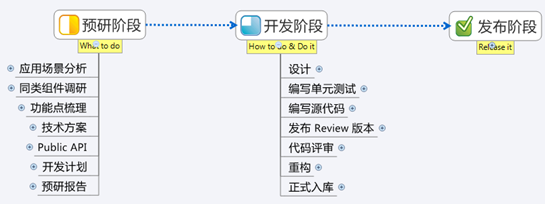
\includegraphics{workflow-s.png}

点击查看详细大图


\subsection{步骤说明}
\label{workflow/workflow-full:id2}
请先阅读 \href{http://kissyteam.github.com/kissy/src/imagezoom/slide.html}{ImageZoom 调研文档}


\subsubsection{应用场景分析}
\label{workflow/workflow-full:id3}
一个需求到来, 比如这个图片放大效果, 首先我们需要这个功能能用在哪些地方, 或哪些网站上已经使用了, 如果有的话, 就对比一下不同的情况下不同的要求, 如 \#slide4 . 这样以后, 对比自己的需求, 想好要实现什么功能, 哪些功能保留, 哪些功能不需要, ---- 明确需求;


\subsubsection{同类组件调研}
\label{workflow/workflow-full:id4}
需求明确之后, 查找现有的同类组件, 看看他们针对这个问题, 是怎么实现的, 实现哪些功能, 哪些可以借鉴的地方, 哪些不足的地方要避免或者改进, 如 \#slide6 , ---- 明确要实现的功能有哪些;


\subsubsection{功能点梳理}
\label{workflow/workflow-full:id5}
分离出完成整个功能需要的几个核心功能点, 并针对各个功能点逐个描述, 如 \#slide8 , 这也可以帮你理清思路,  ---- 进一步明确待实现功能;


\subsubsection{技术方案}
\label{workflow/workflow-full:id6}
针对上述的几个功能点, 分别给出实现方案, 或者其他的技术难点, 又或者是算法上的分析等, 如 \#slide9 , --- 明确如何实现;


\subsubsection{Public API}
\label{workflow/workflow-full:public-api}
设计好的公共 API , 并在此说明, 也可以根据使用场景, 给出一些范例来说明 API 的使用, 如 \#slide14 , 这里可以在开始时设计的尽量精简些, ---- 明确 API 接口;


\subsubsection{开发计划}
\label{workflow/workflow-full:id7}
简略或者详细的制定一个开发计划, 及发布的版本和时间等, ---- 明确进度;


\subsubsection{预研报告}
\label{workflow/workflow-full:id8}
预研过程后总结一个报告, 可将报告分享给大家, 供大家一起讨论.

我们建议每个 KISSY 组件下, 都存放一个 slide.html, 其内容包含上述几部分内容. 这个 slide 随着你的开发过程的推进, 也会不断添加更新, 最后发布时连同组件源代码一起, 形成非常好的知识体系, 这样, 给别人或是几十年后的自己阅读, 也会像看文章一样的有条理.


\section{KISSY 组件开发规范}
\label{workflow/dev-spec:workflow-dev-spec}\label{workflow/dev-spec::doc}\label{workflow/dev-spec:kissy}
by \href{mailto:yiminghe@gmail.com}{承玉}

开始之前请先阅读 {\hyperref[workflow/workflow-simple:workflow-simple]{\emph{KISSY 组件开发流程}}}.


\subsection{确定 API}
\label{workflow/dev-spec:api}
首先确定该组件需要公开的 api 接口包括属性名称, 函数名, 参数以及返回值, 可参考 YUI3 ,Jquery 等类库的同类组件, 尽量保持一致.
比如 Overlay, 那么其公开接口肯定包含方法 \code{show} , \code{hide} 以及弹层内容 \code{content} 属性配置.


\subsection{模块编写}
\label{workflow/dev-spec:id2}
必须. 推荐的目录结构如下, 例如组件为 Overlay 弹层, 那么该组件的目录结构应为:

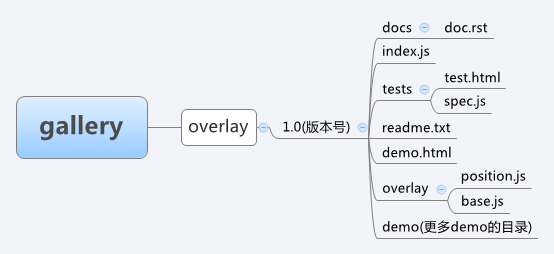
\includegraphics{component-guide.png}

src 目录中必须包含和组件名相同的一个模块文件, 模块名为 \code{gallery/overlay} ,用来指明该组件依赖的子模块, 子模块的名约定为 \code{gallery/overlay/xx} ,如果组件比较简单也可只有这一个源码文件. 例如 overlay.js

\begin{Verbatim}[commandchars=\\\{\}]
\PYG{n+nx}{KISSY}\PYG{p}{.}\PYG{n+nx}{add}\PYG{p}{(}\PYG{l+s+s2}{"gallery/overlay"}\PYG{p}{,}\PYG{k+kd}{function}\PYG{p}{(}\PYG{n+nx}{S}\PYG{p}{,}\PYG{n+nx}{Base}\PYG{p}{)}\PYG{p}{\PYGZob{}}
    \PYG{k}{return} \PYG{n+nx}{Base}\PYG{p}{;}
\PYG{p}{\PYGZcb{}}\PYG{p}{,}\PYG{p}{\PYGZob{}}
    \PYG{l+s+s1}{'./overlay/base'}\PYG{p}{,}\PYG{l+s+s1}{'./overlay/position'}
\PYG{p}{\PYGZcb{}}\PYG{p}{)}\PYG{p}{;}
\end{Verbatim}

子模块放在 \code{src} 模块名为目录名的文件夹内, 对于 KISSY 1.2 以前, 需要手动将组件挂载到 KISSY 上去并且需要在模块定义处挂载, 例如子模块 base.js 的编写:

\begin{Verbatim}[commandchars=\\\{\}]
\PYG{n+nx}{KISSY}\PYG{p}{.}\PYG{n+nx}{add}\PYG{p}{(}\PYG{l+s+s2}{"gallery/overlay/base"}\PYG{p}{,}\PYG{k+kd}{function}\PYG{p}{(}\PYG{n+nx}{S}\PYG{p}{)}\PYG{p}{\PYGZob{}}
    \PYG{k+kd}{function} \PYG{n+nx}{Overlay}\PYG{p}{(}\PYG{p}{)}\PYG{p}{\PYGZob{}}\PYG{p}{\PYGZcb{}}

    \PYG{c+c1}{//如果需要兼容 KISSY \textless{} 1.2, 需要手动挂载到 KISSY}
    \PYG{n+nx}{S}\PYG{p}{.}\PYG{n+nx}{namespace}\PYG{p}{(}\PYG{l+s+s2}{"Gallery"}\PYG{p}{)}\PYG{p}{;}
    \PYG{n+nx}{S}\PYG{p}{.}\PYG{n+nx}{Gallery}\PYG{p}{.}\PYG{n+nx}{Overlay}\PYG{o}{=}\PYG{n+nx}{Overlay}\PYG{p}{;}

    \PYG{k}{return} \PYG{n+nx}{Overlay}\PYG{p}{;}
\PYG{p}{\PYGZcb{}}\PYG{p}{)}\PYG{p}{;}
\end{Verbatim}

子模块间也可有依赖关系, 例如子模块 position.js 需要对基本模块 base.js 进行增强 :

\begin{Verbatim}[commandchars=\\\{\}]
\PYG{n+nx}{KISSY}\PYG{p}{.}\PYG{n+nx}{add}\PYG{p}{(}\PYG{l+s+s2}{"gallery/overlay/position"}\PYG{p}{,}\PYG{k+kd}{function}\PYG{p}{(}\PYG{n+nx}{S}\PYG{p}{,}\PYG{n+nx}{Overlay}\PYG{p}{)}\PYG{p}{\PYGZob{}}
    \PYG{c+c1}{//兼容 kissy \textless{} 1.2}
    \PYG{n+nx}{Overlay} \PYG{o}{=} \PYG{n+nx}{S}\PYG{p}{.}\PYG{n+nx}{Gallery}\PYG{p}{.}\PYG{n+nx}{Overlay}\PYG{p}{;}

    \PYG{n+nx}{Overlay}\PYG{p}{.}\PYG{n+nx}{prototype}\PYG{p}{.}\PYG{n+nx}{xx}\PYG{o}{=}\PYG{k+kd}{function}\PYG{p}{(}\PYG{p}{)}\PYG{p}{\PYGZob{}}\PYG{p}{\PYGZcb{}}\PYG{p}{;}

\PYG{p}{\PYGZcb{}}\PYG{p}{,}\PYG{p}{\PYGZob{}}
    \PYG{n+nx}{requires}\PYG{o}{:}\PYG{p}{[}\PYG{l+s+s1}{'./base'}\PYG{p}{]}
\PYG{p}{\PYGZcb{}}\PYG{p}{)}\PYG{p}{;}
\end{Verbatim}


\subsection{demo 编写}
\label{workflow/dev-spec:demo}
必须. 写一个 \code{demo.html} 简单展示下这个组件怎么用, 静态载入组件的所有依赖js即可, 注意被依赖模块js要放在依赖js前面, 例如:

\begin{Verbatim}[commandchars=\\\{\}]
\PYG{c+cp}{\textless{}!DOCTYPE HTML\textgreater{}}
\PYG{n+nt}{\textless{}html}\PYG{n+nt}{\textgreater{}}
    \PYG{n+nt}{\textless{}head}\PYG{n+nt}{\textgreater{}}
        \PYG{n+nt}{\textless{}title}\PYG{n+nt}{\textgreater{}}overlay demo\PYG{n+nt}{\textless{}/title\textgreater{}}
    \PYG{n+nt}{\textless{}/head\textgreater{}}
    \PYG{n+nt}{\textless{}body}\PYG{n+nt}{\textgreater{}}
        \PYG{n+nt}{\textless{}script }\PYG{n+na}{src=}\PYG{l+s}{'../../../kissy/build/kissy.js'}\PYG{n+nt}{\textgreater{}}\PYG{n+nt}{\textless{}/script\textgreater{}}
        \PYG{n+nt}{\textless{}script }\PYG{n+na}{src=}\PYG{l+s}{'base.js'}\PYG{n+nt}{\textgreater{}}\PYG{n+nt}{\textless{}/script\textgreater{}}
        \PYG{n+nt}{\textless{}script }\PYG{n+na}{src=}\PYG{l+s}{'position.js'}\PYG{n+nt}{\textgreater{}}\PYG{n+nt}{\textless{}/script\textgreater{}}
        \PYG{n+nt}{\textless{}script }\PYG{n+na}{src=}\PYG{l+s}{'overlay.js'}\PYG{n+nt}{\textgreater{}}\PYG{n+nt}{\textless{}/script\textgreater{}}
        \PYG{n+nt}{\textless{}script}\PYG{n+nt}{\textgreater{}}
            \PYG{n+nx}{KISSY}\PYG{p}{.}\PYG{n+nx}{use}\PYG{p}{(}\PYG{l+s+s2}{"gallery/overlay"}\PYG{p}{,}\PYG{k+kd}{function}\PYG{p}{(}\PYG{n+nx}{S}\PYG{p}{,}\PYG{n+nx}{Overlay}\PYG{p}{)}\PYG{p}{\PYGZob{}}
                \PYG{c+c1}{// kissy \textless{} 1.2 获取}
                \PYG{n+nx}{Overlay}\PYG{o}{=}\PYG{n+nx}{S}\PYG{p}{.}\PYG{n+nx}{Gallery}\PYG{p}{.}\PYG{n+nx}{Overlay}\PYG{p}{;}
            \PYG{p}{\PYGZcb{}}\PYG{p}{)}\PYG{p}{;}
        \PYG{n+nt}{\textless{}/script\textgreater{}}
    \PYG{n+nt}{\textless{}/body\textgreater{}}
\PYG{n+nt}{\textless{}/html\textgreater{}}
\end{Verbatim}


\subsection{readme.txt 编写}
\label{workflow/dev-spec:readme-txt}

\subsection{文档编写}
\label{workflow/dev-spec:id3}
可选. 在 \code{docs} 目录下编写组件文档, 后缀名为 \code{rst} , 可参照 \code{KISSY Overlay} 的文档 \href{http://docs.kissyui.com/source/component/overlay/index.rst}{api}  以及
\href{http://docs.kissyui.com/source/component/overlay/usage.rst}{使用文档} , 详细格式可参见 \href{http://sphinx.pocoo.org/}{sphinx} . 文档不做强求, 也可直接写纯文本格式, 在 demo.html 详细讲解即可.


\subsection{单元测试编写}
\label{workflow/dev-spec:id6}
可选. 在 \code{tests} 目录下编写单元测试代码, 单元测试包括两个部分, 测试准备页面以及单元测试用例脚本.


\subsubsection{测试准备页面}
\label{workflow/dev-spec:id7}
编写 test.html , 引入单元测试框架 jasmine (在 kissy/tools/ 下) , 例如:

\begin{Verbatim}[commandchars=\\\{\}]
\PYG{c+cp}{\textless{}!DOCTYPE html\textgreater{}}
\PYG{n+nt}{\textless{}html}\PYG{n+nt}{\textgreater{}}
    \PYG{n+nt}{\textless{}head}\PYG{n+nt}{\textgreater{}}
        \PYG{n+nt}{\textless{}meta} \PYG{n+na}{charset=}\PYG{l+s}{"utf-8"}\PYG{n+nt}{\textgreater{}}
        \PYG{n+nt}{\textless{}title}\PYG{n+nt}{\textgreater{}}Overlay Test Runner\PYG{n+nt}{\textless{}/title\textgreater{}}
        \PYG{n+nt}{\textless{}link} \PYG{n+na}{rel=}\PYG{l+s}{"stylesheet"} \PYG{n+na}{href=}\PYG{l+s}{"../../../tools/jasmine/jasmine.css"}\PYG{n+nt}{\textgreater{}}
        \PYG{n+nt}{\textless{}script }\PYG{n+na}{src=}\PYG{l+s}{"../../../kissy/tools/jasmine/jasmine.js"}\PYG{n+nt}{\textgreater{}}\PYG{n+nt}{\textless{}/script\textgreater{}}
        \PYG{n+nt}{\textless{}script }\PYG{n+na}{src=}\PYG{l+s}{"../../../kissy/tools/jasmine/jasmine-html.js"}\PYG{n+nt}{\textgreater{}}\PYG{n+nt}{\textless{}/script\textgreater{}}
        \PYG{n+nt}{\textless{}script }\PYG{n+na}{src=}\PYG{l+s}{"../../../kissy/tools/jasmine/event-simulate.js"}\PYG{n+nt}{\textgreater{}}\PYG{n+nt}{\textless{}/script\textgreater{}}
        \PYG{n+nt}{\textless{}script }\PYG{n+na}{src=}\PYG{l+s}{"../../../kissy/build/kissy.js"}\PYG{n+nt}{\textgreater{}}\PYG{n+nt}{\textless{}/script\textgreater{}}
    \PYG{n+nt}{\textless{}/head\textgreater{}}
    \PYG{n+nt}{\textless{}body}\PYG{n+nt}{\textgreater{}}
        \PYG{n+nt}{\textless{}script }\PYG{n+na}{src=}\PYG{l+s}{'base.js'}\PYG{n+nt}{\textgreater{}}\PYG{n+nt}{\textless{}/script\textgreater{}}
        \PYG{n+nt}{\textless{}script }\PYG{n+na}{src=}\PYG{l+s}{'position.js'}\PYG{n+nt}{\textgreater{}}\PYG{n+nt}{\textless{}/script\textgreater{}}
        \PYG{n+nt}{\textless{}script }\PYG{n+na}{src=}\PYG{l+s}{'overlay.js'}\PYG{n+nt}{\textgreater{}}\PYG{n+nt}{\textless{}/script\textgreater{}}
        \PYG{n+nt}{\textless{}script }\PYG{n+na}{src=}\PYG{l+s}{"overlay-spec.js"}\PYG{n+nt}{\textgreater{}}\PYG{n+nt}{\textless{}/script\textgreater{}}
        \PYG{n+nt}{\textless{}script}\PYG{n+nt}{\textgreater{}}
            \PYG{n+nx}{jasmine}\PYG{p}{.}\PYG{n+nx}{getEnv}\PYG{p}{(}\PYG{p}{)}\PYG{p}{.}\PYG{n+nx}{addReporter}\PYG{p}{(}\PYG{k}{new} \PYG{n+nx}{jasmine}\PYG{p}{.}\PYG{n+nx}{TrivialReporter}\PYG{p}{(}\PYG{p}{)}\PYG{p}{)}\PYG{p}{;}
            \PYG{n+nx}{jasmine}\PYG{p}{.}\PYG{n+nx}{getEnv}\PYG{p}{(}\PYG{p}{)}\PYG{p}{.}\PYG{n+nx}{execute}\PYG{p}{(}\PYG{k+kd}{function}\PYG{p}{(}\PYG{p}{)} \PYG{p}{\PYGZob{}}
                \PYG{k}{if} \PYG{p}{(}\PYG{n+nx}{parent} \PYG{o}{\&\&} \PYG{n+nx}{parent}\PYG{p}{.}\PYG{n+nx}{jasmine}\PYG{p}{.}\PYG{n+nx}{kissyNext}\PYG{p}{)} \PYG{p}{\PYGZob{}}
                    \PYG{n+nx}{parent}\PYG{p}{.}\PYG{n+nx}{jasmine}\PYG{p}{.}\PYG{n+nx}{kissyNext}\PYG{p}{(}\PYG{k}{this}\PYG{p}{.}\PYG{n+nx}{results}\PYG{p}{(}\PYG{p}{)}\PYG{p}{.}\PYG{n+nx}{failedCount}\PYG{p}{)}\PYG{p}{;}
                \PYG{p}{\PYGZcb{}}
            \PYG{p}{\PYGZcb{}}\PYG{p}{)}\PYG{p}{;}
        \PYG{n+nt}{\textless{}/script\textgreater{}}
    \PYG{n+nt}{\textless{}/body\textgreater{}}
\PYG{n+nt}{\textless{}/html\textgreater{}}
\end{Verbatim}


\subsubsection{测试用例脚本编写}
\label{workflow/dev-spec:id8}
测试用例编写在脚本 \code{overlay-spec.js} 中, 详细可参考 \href{https://github.com/pivotal/jasmine/wiki}{jasmine wiki} , 这里简单举个例子:

\begin{Verbatim}[commandchars=\\\{\}]
\PYG{c+c1}{// 测试用例脚本可以包含很多 suit}
\PYG{n+nx}{describe}\PYG{p}{(}\PYG{l+s+s2}{"开始一个 suit"}\PYG{p}{,}\PYG{k+kd}{function}\PYG{p}{(}\PYG{p}{)}\PYG{p}{\PYGZob{}}

    \PYG{c+c1}{// 一个 suit 包含很多 spec}
    \PYG{n+nx}{it}\PYG{p}{(}\PYG{l+s+s2}{"开始一个 spec"}\PYG{p}{,}\PYG{k+kd}{function}\PYG{p}{(}\PYG{p}{)}\PYG{p}{\PYGZob{}}

        \PYG{c+cm}{/*}
\PYG{c+cm}{            一个 spec 包含很多 expectation}
\PYG{c+cm}{        */}
        \PYG{n+nx}{expect}\PYG{p}{(}\PYG{l+s+s2}{"xx"}\PYG{p}{)}\PYG{p}{.}\PYG{n+nx}{toBe}\PYG{p}{(}\PYG{l+s+s2}{"xx"}\PYG{p}{)}\PYG{p}{;}
        \PYG{n+nx}{expect}\PYG{p}{(}\PYG{l+s+s2}{"yy"}\PYG{p}{)}\PYG{p}{.}\PYG{n+nx}{toBe}\PYG{p}{(}\PYG{l+s+s2}{"yy"}\PYG{p}{)}\PYG{p}{;}

    \PYG{p}{\PYGZcb{}}\PYG{p}{)}\PYG{p}{;}

\PYG{p}{\PYGZcb{}}\PYG{p}{)}\PYG{p}{;}
\end{Verbatim}

复杂点的例子可以看 \href{https://github.com/kissyteam/kissy/blob/master/src/overlay/tests/overlay-spec.js}{KISSY.Overlay Unit Test}


\renewcommand{\indexname}{Python Module Index}
\begin{theindex}
\def\bigletter#1{{\Large\sffamily#1}\nopagebreak\vspace{1mm}}
\bigletter{a}
\item {\texttt{Accordion}}, \pageref{api/component/switchable/accordion:module-Accordion}
\item {\texttt{Anim}}, \pageref{api/core/anim/index:module-Anim}
\item {\texttt{attribute}}, \pageref{api/core/base/index:module-attribute}
\indexspace
\bigletter{c}
\item {\texttt{Calendar}}, \pageref{api/component/calendar/index:module-Calendar}
\item {\texttt{Carousel}}, \pageref{api/component/switchable/carousel:module-Carousel}
\item {\texttt{cookie}}, \pageref{api/core/cookie/index:module-cookie}
\indexspace
\bigletter{d}
\item {\texttt{DataLazyload}}, \pageref{api/component/datalazyload/index:module-DataLazyload}
\item {\texttt{DDM}}, \pageref{api/component/dd/ddm:module-DDM}
\item {\texttt{DOM}}, \pageref{api/core/dom/index:module-DOM}
\item {\texttt{Draggable}}, \pageref{api/component/dd/draggable:module-Draggable}
\item {\texttt{DraggableDelegate}}, \pageref{api/component/dd/draggable-delegate:module-DraggableDelegate}
\item {\texttt{Droppable}}, \pageref{api/component/dd/droppable:module-Droppable}
\item {\texttt{DroppableDelegate}}, \pageref{api/component/dd/droppable-delegate:module-DroppableDelegate}
\indexspace
\bigletter{e}
\item {\texttt{Editor}}, \pageref{relatedproj/editorguide/index:module-Editor}
\item {\texttt{Event}}, \pageref{api/core/event/index:module-Event}
\indexspace
\bigletter{f}
\item {\texttt{flash}}, \pageref{api/component/flash/index:module-flash}
\indexspace
\bigletter{i}
\item {\texttt{ImageZoom}}, \pageref{api/component/imagezoom/index:module-ImageZoom}
\item {\texttt{io}}, \pageref{api/core/ajax/index:module-io}
\indexspace
\bigletter{j}
\item {\texttt{json}}, \pageref{api/core/json/index:module-json}
\indexspace
\bigletter{l}
\item {\texttt{Lang}}, \pageref{api/seed/lang/index:module-Lang}
\item {\texttt{Loader}}, \pageref{api/seed/loader/index:module-Loader}
\indexspace
\bigletter{m}
\item {\texttt{module-compiler}}, \pageref{tools/module-compiler/index:module-module-compiler}
\indexspace
\bigletter{n}
\item {\texttt{Node}}, \pageref{api/core/node/index:module-Node}
\indexspace
\bigletter{o}
\item {\texttt{Overlay}}, \pageref{api/component/overlay/popup:module-Overlay}
\indexspace
\bigletter{p}
\item {\texttt{Proxy}}, \pageref{api/component/dd/proxy:module-Proxy}
\indexspace
\bigletter{s}
\item {\texttt{Scroll}}, \pageref{api/component/dd/scroll:module-Scroll}
\item {\texttt{Seed}}, \pageref{api/seed/kissy/index:module-Seed}
\item {\texttt{Slide}}, \pageref{api/component/switchable/slide:module-Slide}
\item {\texttt{Suggest}}, \pageref{api/component/suggest/index:module-Suggest}
\item {\texttt{Switchable}}, \pageref{api/component/switchable/switchable:module-Switchable}
\indexspace
\bigletter{t}
\item {\texttt{Tabs}}, \pageref{api/component/switchable/tabs:module-Tabs}
\item {\texttt{Template}}, \pageref{api/component/template/index:module-Template}
\indexspace
\bigletter{u}
\item {\texttt{UA}}, \pageref{api/core/ua/index:module-UA}
\indexspace
\bigletter{w}
\item {\texttt{Web}}, \pageref{api/seed/web/index:module-Web}
\end{theindex}

\renewcommand{\indexname}{Index}
\printindex
\end{document}
